% !TeX program = lualatex
% !BIB program = biber
\documentclass[
  11pt,
%  left=12.7mm
%  right=6.35mm
%  top=6.35mm
%  bottom=6.35mm
  a4paper,
  twoside=true,
  open=right,
  headings=big,
  numbers=noenddot,
  bibliography=totoc,
  index=totoc,
  listof=totoc,
  BCOR=8mm,
  DIV=12
]{scrbook}

% ============================================================
% PowerSystemBook 3.2 -- central preamble
% Engine: LuaLaTeX | Bibliography: Biber | Index: MakeIndex
% ============================================================

% 1. Language, fonts, typography
\usepackage[english]{babel}
\usepackage{csquotes}
\usepackage{fontspec}
\usepackage{unicode-math}
\usepackage{microtype}
\setmainfont{Libertinus Serif}
\setsansfont{Libertinus Sans}
\setmonofont{Libertinus Mono}[Scale=MatchLowercase]
\setmathfont{Libertinus Math}
\setlength{\emergencystretch}{2em}
\raggedbottom

% 2. Colour palette
\usepackage{xcolor}
\definecolor{BookBlue}{RGB}{24,72,120}
\definecolor{BookBlueDark}{RGB}{17,50,84}
\definecolor{BookGreen}{RGB}{42,105,70}
\definecolor{BookOrange}{RGB}{181,105,22}
\definecolor{BookRed}{RGB}{155,45,45}
\definecolor{BookGray}{RGB}{88,92,96}
\definecolor{LightBlue}{RGB}{241,247,252}
\definecolor{LightGreen}{RGB}{242,249,244}
\definecolor{LightYellow}{RGB}{255,249,230}
\definecolor{LightRed}{RGB}{253,242,242}
\definecolor{LightGray}{RGB}{246,247,248}
% Formula-sheet colours (formerly defined locally in the appendices).
\definecolor{navy}{HTML}{17365D}
\definecolor{blue}{HTML}{2F75B5}
\definecolor{sky}{HTML}{EAF3FA}
\definecolor{gold}{HTML}{D69E2E}
\definecolor{ink}{HTML}{243447}
\definecolor{muted}{HTML}{617285}
\definecolor{shadecolor}{HTML}{F1F6FA}

% 3. Mathematics and units
\usepackage{amsmath,mathtools,bm}
\usepackage{siunitx}
\DeclareSIUnit{\varunit}{var}
\DeclareSIUnit{\rpm}{rpm}
\DeclareSIUnit{\pu}{p.u.}
\sisetup{
  per-mode=symbol,
  separate-uncertainty=true,
  detect-all,
  exponent-product=\cdot,
  output-decimal-marker={.},
  group-minimum-digits=4
}
\newcommand{\vect}[1]{\bm{#1}}
\newcommand{\mat}[1]{\bm{#1}}
\newcommand{\e}{\mathrm{e}}
\newcommand{\imag}{\mathrm{j}}
\newcommand{\diff}{\mathop{}\!\mathrm{d}}
\newcommand{\Rmag}{\mathcal{R}}
\newcommand{\sign}{\operatorname{sign}}
\newcommand{\eqsep}{\addlinespace[2pt]}
\newcommand{\formulaTableStretch}{1.18}

% 4. Graphics, plots, captions, tables
\usepackage{graphicx}
\usepackage{tikz}
\graphicspath{{figures/}{figures/common/}{figures/transformers/}{figures/lines/}{figures/generators/}}
\usepackage{float}
\usepackage{subcaption}
\usepackage{booktabs,longtable,tabularx,array,multirow}
\usepackage{placeins}
\usepackage{pdflscape}
\usepackage{framed}

% Full-page landscape figure.
% Usage:
% \begin{widefigure}{Caption text}{fig:label}
%   \includegraphics[width=.95\linewidth]{drawing.pdf}
% \end{widefigure}
\NewDocumentEnvironment{widefigure}{O{p} m m}{%
  \begin{landscape}%
  \begin{figure}[#1]%
  \centering
}{%
  \caption{#2}%
  \label{#3}%
  \end{figure}%
  \end{landscape}%
}
\captionsetup{
  font=small,
  labelfont={bf,color=BookBlueDark},
  textfont=small,
  justification=raggedright,
  singlelinecheck=false,
  skip=6pt
}
\renewcommand{\arraystretch}{1.15}
\newcolumntype{Y}{>{\raggedright\arraybackslash}X}

% 5. Lists
\usepackage{enumitem}
\setlist{topsep=4pt,itemsep=2pt,parsep=0pt}
\setlist[itemize,1]{label=\textcolor{BookBlue}{\small\textbullet}}

% 6. Page design, headings, headers and footers
\usepackage[automark,headsepline=.4pt]{scrlayer-scrpage}
\setkomafont{pageheadfoot}{\small\sffamily\color{BookGray}}
\setkomafont{pagenumber}{\bfseries\color{BookBlueDark}}
\clearpairofpagestyles
\ihead{\headmark}
\ohead{\pagemark}
\ifoot{Friedrich Schmidt}
\ofoot{Power System Simulation with LTspice}
\pagestyle{scrheadings}
\renewcommand*{\chapterpagestyle}{plain}

\setkomafont{chapter}{\normalfont\sffamily\bfseries\color{BookBlueDark}}
\setkomafont{section}{\normalfont\sffamily\bfseries\color{BookBlue}}
\setkomafont{subsection}{\normalfont\sffamily\bfseries\color{BookBlueDark}}
\setkomafont{disposition}{\normalfont\sffamily\bfseries}
\RedeclareSectionCommand[beforeskip=0pt,afterskip=1.4\baselineskip]{chapter}
\RedeclareSectionCommand[beforeskip=1.7\baselineskip,afterskip=.55\baselineskip]{section}
\RedeclareSectionCommand[beforeskip=1.3\baselineskip,afterskip=.4\baselineskip]{subsection}

% 7. Hyperlinks and cross-references
\usepackage{hyperref}
\hypersetup{
  colorlinks=true,
  linkcolor=BookBlueDark,
  citecolor=BookGreen,
  urlcolor=BookBlue,
  pdfborder={0 0 0},
  pdftitle={Power System Simulation with LTspice},
  pdfauthor={Friedrich Schmidt},
  pdfsubject={Power-system modelling and simulation}
}
\usepackage[nameinlink,noabbrev,capitalise]{cleveref}

% 8. Instructional boxes
% Robust tcolorbox setup for MiKTeX/LuaLaTeX.
% Deliberately no "most", "skins", "enhanced" or TikZ "fadings" library.
\usepackage{tcolorbox}
\tcbuselibrary{breakable,theorems}

% Common appearance: rounded corners, integrated coloured title bar,
% thin frame, generous spacing and automatic page breaks.
\tcbset{
  bookbox/.style={
    breakable,
    boxrule=.55pt,
    arc=1.6mm,
    outer arc=1.6mm,
    left=3.5mm,
    right=3.5mm,
    top=3.0mm,
    bottom=3.0mm,
    before skip=12pt,
    after skip=12pt,
    fonttitle=\sffamily\bfseries,
    coltitle=white,
    separator sign={\enspace--},
    description delimiters parenthesis,
    before upper={\setlength{\parindent}{0pt}},
    titlerule=.4pt
  }
}

\newtcbtheorem[number within=chapter]{definition}{Definition}{
  bookbox,
  colback=LightBlue,
  colframe=BookBlue,
  colbacktitle=BookBlue
}{def}

\newtcbtheorem[number within=chapter]{remark}{Remark}{
  bookbox,
  colback=LightGray,
  colframe=BookGray,
  colbacktitle=BookGray
}{rem}

\newtcbtheorem[number within=chapter]{example}{Example}{
  bookbox,
  colback=LightGreen,
  colframe=BookGreen,
  colbacktitle=BookGreen
}{ex}

\newtcbtheorem[number within=chapter]{important}{Important}{
  bookbox,
  colback=LightRed,
  colframe=BookRed,
  colbacktitle=BookRed
}{imp}

\newtcbtheorem[number within=chapter]{simulation}{Simulation}{
  bookbox,
  colback=white,
  colframe=BookBlue,
  colbacktitle=BookBlue
}{sim}

\newtcbtheorem[number within=chapter]{calculation}{Calculation}{
  bookbox,
  colback=white,
  colframe=BookOrange,
  colbacktitle=BookOrange,
  before upper={
    \setlength{\parindent}{0pt}
    \setlength{\abovedisplayskip}{6pt}
    \setlength{\belowdisplayskip}{6pt}
  }
}{calc}

\newtcbtheorem[number within=chapter]{result}{Result}{
  bookbox,
  colback=LightGreen,
  colframe=BookGreen,
  colbacktitle=BookGreen,
  fontupper=\bfseries
}{res}

\newtcolorbox{chaptersummary}[1][Chapter Summary]{
  bookbox,
  title={#1},
  colback=LightBlue,
  colframe=BookBlueDark,
  colbacktitle=BookBlueDark,
  before upper={
    \setlength{\parindent}{0pt}
    \setlength{\parskip}{.4\baselineskip}
  }
}

\newtcolorbox{warningbox}[1][Warning]{
  bookbox,
  title={#1},
  colback=LightRed,
  colframe=BookRed,
  colbacktitle=BookRed
}

% Formula sheets: lightweight, fading-free design based on the transformer
% appendix.  Both formula appendices use only these central definitions.
\newenvironment{formulaBox}[1]{%
  \par\medskip
  {\sffamily\bfseries\large\color{navy}#1}\par\nobreak\smallskip
  \def\FrameCommand{\hspace{1pt}{\color{blue}\vrule width 2.2pt}\hspace{8pt}}%
  \MakeFramed{\advance\hsize-11.2pt\FrameRestore}%
  \setlength{\parindent}{0pt}\setlength{\parskip}{5pt}%
}{\endMakeFramed\par\smallskip}

\newenvironment{noteBox}{%
  \par\smallskip
  \def\FrameCommand{\hspace{1pt}{\color{gold}\vrule width 2.2pt}%
    \colorbox{shadecolor}}%
  \MakeFramed{\advance\hsize-2\width\advance\hsize-2\fboxsep\FrameRestore}%
  \setlength{\parindent}{0pt}\setlength{\parskip}{5pt}%
}{\endMakeFramed\par\smallskip}

\newcommand{\formulasheettitle}[2]{%
  \refstepcounter{chapter}%
  \addcontentsline{toc}{chapter}{\protect\numberline{\thechapter}#1}%
  \markboth{#1}{Formula sheet}%
  \begingroup
  \setlength{\fboxsep}{8mm}%
  \noindent\colorbox{navy}{%
    \parbox{\dimexpr\textwidth-2\fboxsep\relax}{%
      {\sffamily\bfseries\fontsize{25}{29}\selectfont\color{white}#1}\par
      \vspace{2mm}%
      {\sffamily\fontsize{15}{18}\selectfont\color{white!85}#2}%
    }}%
  \endgroup
  \vspace{3mm}%
}

\crefname{definition}{definition}{definitions}
\crefname{remark}{remark}{remarks}
\crefname{example}{example}{examples}
\crefname{important}{important note}{important notes}
\crefname{simulation}{simulation}{simulations}
\crefname{calculation}{calculation}{calculations}
\crefname{result}{result}{results}

% 9. MATLAB, LTspice and generic code listings
\usepackage{listings}
\renewcommand{\lstlistlistingname}{List of Listings}
\renewcommand{\lstlistingname}{Listing}
\lstdefinestyle{CommonCode}{
  basicstyle=\ttfamily\small,
  numbers=left,numberstyle=\scriptsize\color{BookGray},numbersep=8pt,
  frame=single,framerule=.4pt,rulecolor=\color{BookGray},
  backgroundcolor=\color{LightGray},
  breaklines=true,breakatwhitespace=false,
  showstringspaces=false,tabsize=4,columns=fullflexible,keepspaces=true,
  aboveskip=10pt,belowskip=10pt,
  captionpos=b
}
\lstdefinestyle{Matlab}{style=CommonCode,language=Matlab,keywordstyle=\bfseries\color{BookBlue},commentstyle=\itshape\color{BookGreen},stringstyle=\color{BookOrange}}
\lstdefinestyle{LTspice}{style=CommonCode,numbers=none,numbersep=0pt,morecomment=[l]{*},morecomment=[l]{;},keywordstyle=\bfseries\color{BookBlue}}
\lstdefinestyle{PlainText}{style=CommonCode,numbers=none}

% 10. Bibliography
\usepackage[backend=biber,style=ieee,sorting=none,maxbibnames=99]{biblatex}
\addbibresource{bibliography.bib}

% 11. Index and document depth
\usepackage{imakeidx}
\makeindex[title=Index,intoc]
\setcounter{tocdepth}{2}
\setcounter{secnumdepth}{3}
\listfiles


\begin{document}

% ============================================================
% Front matter: Roman page numbers
% ============================================================
\frontmatter
\pagestyle{plain}
%\begin{titlepage}
	\thispagestyle{empty}
	
	\begin{tikzpicture}[remember picture,overlay]
		
		% Großer dunkelblauer Titelbereich
		\fill[BookBlueDark]
		(current page.north west)
		rectangle ([yshift=-105mm]current page.north east);
		
		% Schmaler Akzentbalken
		\fill[BookBlue]
		([yshift=-105mm]current page.north west)
		rectangle ([yshift=-109mm]current page.north east);
		
		% Titel unabhängig von den normalen Seitenrändern positionieren
		\node[
		anchor=north west,
		align=left,
		text=white,
		text width=150mm,
		inner sep=0pt
		] at ([xshift=28mm,yshift=-27mm]current page.north west) {%
			{\sffamily\bfseries\fontsize{30}{36}\selectfont
				Power System Simulation\par}
			
			\vspace{3mm}
			
			{\sffamily\bfseries\fontsize{25}{31}\selectfont
				with LTspice\par}
			
			\vspace{11mm}
			
			{\sffamily\Large
			A practical approach to power system simulation\par}
		};
		
		% Autor und Versionsangabe am unteren Seitenrand
		\node[
		anchor=south west,
		align=left,
		text width=150mm,
		inner sep=0pt
		] at ([xshift=28mm,yshift=27mm]current page.south west) {%
			{\sffamily\Large Friedrich Schmidt\par}
			
			\vspace{7mm}
			
			{\sffamily\large Version 1.0 \par}
		};
		
	\end{tikzpicture}
	
	\null
\end{titlepage}
\cleardoublepage

\thispagestyle{empty}
\vspace*{\fill}
\noindent\textbf{Power System Simulation with LTspice}\\
A practical approach to power system simulation\\[1.5em]
%ISBN 978-102-304-186\\[1.5em]
Copyright \textcopyright\ 2026 Friedrich Schmidt.\\[1em]
All rights reserved. No part of this publication may be reproduced or distributed without permission of the copyright holder, except where permitted by law.\\[1em]
The software names and trademarks mentioned in this book remain the property of their respective owners. The examples are provided for educational purposes. Users are responsible for validating models and results for their own applications. There is no responsibility using this toolbox\\[2em]
First working edition, 2026.
%\cleardoublepage
\newpage

\thispagestyle{empty}
\vspace*{0.35\textheight}
\begin{center}
\itshape
For everyone who wants to gain a deeper understanding of power systems.\newline
\end{center}
%\cleardoublepage
\newpage
\chapter*{Preface}
\addcontentsline{toc}{chapter}{Preface}
This book presents practical methods for modelling and analysing electrical power systems with LTspice. The emphasis is placed on reproducible examples that connect physical interpretation, manual calculation and numerical simulation.

The material is intended for students, engineers and technically interested readers. Each chapter combines a concise theoretical introduction with worked calculations, circuit models, simulation results and practical remarks.

The book presents nine simulation examples, ranging from simple to more complex cases. The formatting of the book and, in some cases, the translation from German to English were done with the help of ChatGPT. All examples and technical details are, of course, provided by the author. I wish readers every success with their simulations and hope that they, too—like me—will find great enjoyment in them.
I would also like to thank the developers of LTspice for this excellent software, which made it possible for me to write this book. Although it is designed for simulating electronic circuits, it is so flexible that it allowed me to perform high-voltage analyses with it as well. Using a mathematical trick, I was also able to adapt LTspice for steady-state load-flow calculations, which led to the development of my second toolbox. This toolbox is also freely available and will be presented in more detail in a future book.

LTspice is a simulator developed by Analog Devices and is available free of charge. Having worked for more than 35 years as a load dispatcher in Vienna’s electricity distribution system, I have drawn on my practical experience in developing these toolboxes.
I hope that you enjoy exploring electrical power systems through simulation as much as I do. Some simulations can be challenging, but the results offer valuable insights. Good luck with your simulations!

\vspace{2cm}
\begin{flushright}
Friedrich Schmidt\\
Austria, July 2026
\end{flushright}
%\cleardoublepage
\newpage
\chapter*{Acknowledgements}
\addcontentsline{toc}{chapter}{Acknowledgements}
I would like to express my sincere thanks for the excellent examples in the book "Dynamisches Verhalten elektrischer Maschinen" by Prof. Otto Justus, which provided me with a great deal of inspiration for my own book.
%\cleardoublepage
\newpage
\chapter*{How to Use This Book}
\addcontentsline{toc}{chapter}{How to Use This Book}
The chapters are written so that the reader can reproduce the examples directly. The following elements are used consistently:
\begin{description}[style=nextline,leftmargin=32mm]
	\item[Introduction] Introduces the examples
	\item[Remark] Adds interpretation, limitations or practical advice.
	\item[Example] Presents a worked application.
	\item[Calculation] Aligns formulas, substituted values and results.
	\item[Simulation] Describes model settings and simulation steps.
	\item[Chapter Summary] Collects the main conclusions at the end of a chapter.
\end{description}
 
\vspace{11mm}

It is recommended that you work through the book from beginning to end, while reproducing the examples in LTspice. A prerequisite for successful simulations is a good understanding of how to use the LTspice simulator. A solid understanding of SPICE syntax is absolutely essential for a thorough understanding of how the models are constructed.
The complex models of the transformer and the synchronous generator are explained in the appendices of this book. To better understand the detailed modeling, it is recommended to review the LTspice-library files.

The free software WxMaxima was used in the book for simple calculations. The free software GeoGebra was used to construct the vector diagrams. In the “coupled lines” section, the Atp (Atpdraw) program was used for the overhead line model; however, it is not required for the simulation.

%\cleardoublepage
%\chapter*{Symbols and Units}
\addcontentsline{toc}{chapter}{Symbols and Units}
\begin{longtable}{@{}>{$}l<{$} p{0.58\textwidth} l@{}}
\toprule
\textnormal{Symbol} & Description & Unit \\
\midrule
\endfirsthead
\toprule
\textnormal{Symbol} & Description & Unit \\
\midrule
\endhead
R & Electrical resistance & \si{\ohm} \\
L & Inductance & \si{\henry} \\
C & Capacitance & \si{\farad} \\
X & Reactance & \si{\ohm} \\
Z & Impedance & \si{\ohm} \\
U & Voltage, RMS value unless otherwise stated & \si{\volt} \\
I & Current, RMS value unless otherwise stated & \si{\ampere} \\
P & Active power & \si{\watt} \\
Q & Reactive power & \si{\varunit} \\
S & Apparent power & \si{\volt\ampere} \\
f & Frequency & \si{\hertz} \\
\omega & Angular frequency & \si{\radian\per\second} \\
\bottomrule
\end{longtable}
\cleardoublepage

%\chapter*{Abbreviations}
\addcontentsline{toc}{chapter}{Abbreviations}
\begin{longtable}{@{}lp{0.72\textwidth}@{}}
\toprule
Abbreviation & Meaning \\
\midrule
AC & Alternating current \\
DC & Direct current \\
EMT & Electromagnetic transients \\
HVDC & High-voltage direct current \\
OLTC & On-load tap changer \\
RMS & Root mean square \\
TOV & Temporary overvoltage \\
\bottomrule
\end{longtable}
\cleardoublepage


\tableofcontents
\cleardoublepage
\listoffigures
\cleardoublepage
\listoftables
\cleardoublepage
\lstlistoflistings
\cleardoublepage

% ============================================================
% Main matter: Arabic page numbers
% ============================================================
\mainmatter
\pagestyle{scrheadings}
\chapter{Transformer and Shunt Reactor}
\label{chap:transformer-shunt-reactor}
\index{transformer}
\index{shunt reactor}

\section{General}
\label{sec:tsr-general}

In the first example, a three-phase circuit is examined. The case of an inductive load, namely the switching-on of a shunt reactor, and its impact on the voltage are investigated. The load is energized first by one transformer and then by two transformers. Finally, a special case with two transformers in series is presented. Such a configuration can occur when a de-energized part of a network is restored from a network section that is already energized (for instance after a blackout).


\section{Circuit Design}
\label{sec:tsr-circuit-design}
The example file \texttt{Transformer\_and\_shunt\_reactor.asc} is for the first transient (.TRAN) analysis. 
Additional measurements defined with \texttt{.meas} in the LTspice schematic are written to the \texttt{spice-output-logfile} file at the end of the simulation. In LTspice, this file can be opened with \emph{View~$\rightarrow$~SPICE Output Log}. 
To set simulation accuracy for voltages and currents the LTspice netlist settings are:\\ 

\begin{lstlisting}[style=LTspice]
	.options vntol=1m
	.options abstol=1u
\end{lstlisting}

\noindent These values are much higher as at normal LTspice simulations with electronic circuits.

\begin{remark}{Convergence}{Remark11}
	If you encounter convergence problems you can try to increase \texttt{vntol} and \texttt{abstol}.
	You can also try to set the relative tolerance \texttt{reltol} to 0.01
	Changing the default integration mode can also be helpful.
\end{remark}

\noindent The following line for frequency and angular velocity should be included in every schematic:\\

\begin{lstlisting}[style=LTspice]
	.param tdv=1 tdt=1 fn1=50Hz(60Hz) omega_n={2*pi*fn1}
\end{lstlisting}

\noindent tdv=1 and tdt=1 are LTspice parameters used to avoid convergence problems with electrical power networks.
This first example contains buses, an impedance, transformers, and shunt reactors. The bus elements provide external measurement pins and the setting for the line-to-line voltage. Elements with three pins, such as \texttt{bus\_v}, measure all three line-to-line voltages as instantaneous values (bus\_v) or RMS values (bus\_Veff). During simulation the RMS values require some time to settle.

For modeling the net-impedance the model impedance\_sk is used. The model use nominal voltage and short-circuit power as inputs, assuming equal values for all phases. The values for SN and UN should be:\\
\newpage

\begin{lstlisting}[style=LTspice]
SN=40e9
UN=400k
\end{lstlisting}

The transformer model used in this circuit is a simple linear model without a magnetic core, because a nonlinear core is not required for this example. After placing the symbol \texttt{trafo\_yy}, the model \texttt{RUYy0\_400k\_120k\_300MVA\_simple} is selected in the SpiceModel field (double-click to open the drop-down list) in the attribute editor. Other default parameter lines are removed.\\

The three-phase voltage source is started with exponential damping using the parameter \texttt{Texp=50ms}. This accelerates the settling of the current of the shunt reactor. The shunt reactor has a rating of \SI{50}{\mega\varunit} and a nominal voltage of \SI{110}{\kilo\volt}. Its nominal current is approximately \SI{250}{\ampere} RMS. The total simulation time is set to \SI{4}{\second}.

\noindent This is set by the .tran command of LTspice

\begin{lstlisting}[style=LTspice]
.tran 0 4s 0m 0.1m
\end{lstlisting}
A value of 0.1m specifies a maximum time step of 0.1 ms, which should be sufficiently small to resolve 50 Hz or 60 Hz sinusoidal waveforms accurately. Use a smaller time step for higher frequencies. For the following four examples the ltspice file is 
\texttt{Transformer\_and\_shunt\_reactor.asc}

\subsection{Transformer Without Shunt Reactor}
\label{sec:without-shunt-reactor}

The voltage at the bus is approximately \SI{119.7}{\kilo\volt}. Thus, the nominal voltage of \SI{120}{\kilo\volt} is nearly reached. The small difference is caused by the series impedance of the network, which slightly reduces the voltage. 

\subsection{One Transformer and Shunt Reactor}
\label{sec:one-transformer-shunt-reactor}

In this case, the shunt reactor reduces the voltage to approximately \SI{115.1}{\kilo\volt}. The RMS current is approximate \SI{275}{\ampere}. This is higher than the rough estimate of \SI{250}{\ampere}, because the operating voltage is higher than the nominal voltage of the shunt reactor.

\subsection{Two Transformers in Parallel and Shunt Reactor}
\label{sec:parallel-transformers-shunt-reactor}

With two transformers connected in parallel, the equivalent internal impedance is reduced by a factor of two. Consequently, the voltage drop is smaller, and the voltage reaches approximately \SI{117.3}{\kilo\volt}. The current through the shunt reactor increases to approximately \SI{280}{\ampere} because of the higher operating voltage.

\subsection{Two Transformers in Series and Shunt Reactor}
\label{sec:series-transformers-shunt-reactor}

The shunt reactor is now supplied from a \SI{120}{\kilo\volt} source through two transformers connected in series. The transformer impedance is therefore doubled, and the voltage is reduced from \SI{119.2}{\kilo\volt} to approximately \SI{110.5}{\kilo\volt} corresponding to a voltage drop of \SI{8.7}{\kilo\volt}. The shunt-reactor current is approximately \SI{264}{\ampere}.
This configuration can arise when a de-energized part of a network is restored from a network section that remains energized (for instance after a blackout). Because of the large combined transformer impedance, the voltage is particularly sensitive to load changes in this configuration.

\subsection{Transformer and Shunt Reactor for AC-Analysis}
\noindent For an AC analysis the filename of the example is \texttt{Transformer\_and\_shunt\_reactor\_AC.asc}.
For the AC analysis, the voltage-source model is changed to \texttt{V\_3phase\_AC}. The transient-analysis directive \texttt{.tran} is replaced by an \texttt{.ac} directive. For measuring the bus voltages
the transient bus models must be replaced with the appropriate ac bus models \texttt{bus\_V} with \texttt{bus\_V\_AC} to measure line to line voltages and \texttt{bus\_Veff} with \texttt{bus\_V0\_AC} to measure line to earth voltages.

\begin{important}{AC-Analysis}{important11}
	Linear AC analysis linearizes nonlinear elements at the operating point and is therefore not suitable for large-signal analysis.
\end{important}

%\noindent On the next page Figure~\ref{fig:schematic1} shows the Schematic for the Transformer and shunt %reactor AC example and ..\\

%\noindent .. on the following page Figure~\ref{fig:Transformer_and_shunt_reactor_AC_Waveform} shows the %steady-state AC phase voltages together with the currents flowing through the shunt reactors.\\

%\begin{example}{Transformer and shuntreactor AC}{}
%	Shows the schematic and output of the waveformviewer for AC-Analysis
%\end{example}


%\vspace{0.1pt}

\section{Manual Calculation of the Line-to-Line Voltage Drop with Two Transformers in Series}
\label{sec:manual-calculation-series-case}

	The internal impedance of a \SI{400}{\kilo\volt}/\SI{120}{\kilo\volt} transformer is approximately \SI{9.6}{\ohm} inductive when referred to the secondary side. (See equation ~\ref{eq:eqn1_9}). For two transformers connected in series, the total impedance is therefore approximately

\begin{calculation}{Voltage reduction}{calculation11}

	\begin{align}
		X_{\mathrm{T,tot}} &= 2 \cdot \SI{9.6}{\ohm}
		= \SI{19.2}{\ohm}.
	\end{align}
	
	With a current of approximately \SI{264}{\ampere}, the phase-voltage drop is
	
	\begin{align}
		\Delta U_{\mathrm{ph}}
		&= I X_{\mathrm{T,tot}} \\
		&= \SI{264}{\ampere} \cdot \SI{19.2}{\ohm} \\
		&= \SI{5}{\kilo\volt}.
	\end{align}
	
	The corresponding line-to-line voltage drop is approximately
	
    \begin{align}
	\Delta U_{\mathrm{LL}}
	&= \sqrt{3}\,\Delta U_{\mathrm{ph}} \\
	&\approx 1.73 \cdot \SI{5}{\kilo\volt} \\
%	&\approx \SI{8.65}{\kilo\volt}.
    &\approx\boxed{\mathbf{\SI{8.65}{\kilo\volt}}}
    \end{align}
	
	This result agrees well with the simulated voltage reduction in \cref{sec:series-transformers-shunt-reactor}.\\
\end{calculation}



\noindent To get the value of the leakage impedance of transformer 
we can see the wxmaxima file \texttt{transformer\_400kV\_120kV\_yy.wxmx} and search for xkus.

\begin{calculation}{Leakage impedance}{calculation12}
    \begin{align}
	X_{1\mathrm{s}}
	&= L_{1\mathrm{s}}\,\omega \nonumber\\
	&= 0.1697 \cdot 314.159 \nonumber\\
	&= \SI{53.33}{\ohm} \\[2ex]
	X_{2\mathrm{s}}
	&= X_{1\mathrm{s}}
	\frac{(\SI{120}{\kilo\volt})^{2}}
	{(\SI{400}{\kilo\volt})^{2}}
	\nonumber\\
	&= \boxed{\mathbf{\SI{9.60}{\ohm}}} 
	\label{eq:eqn1_9}
%	&= \SI{9.60}{\ohm}
    \end{align}
\end{calculation}

\begin{figure}[H]
	\centering
    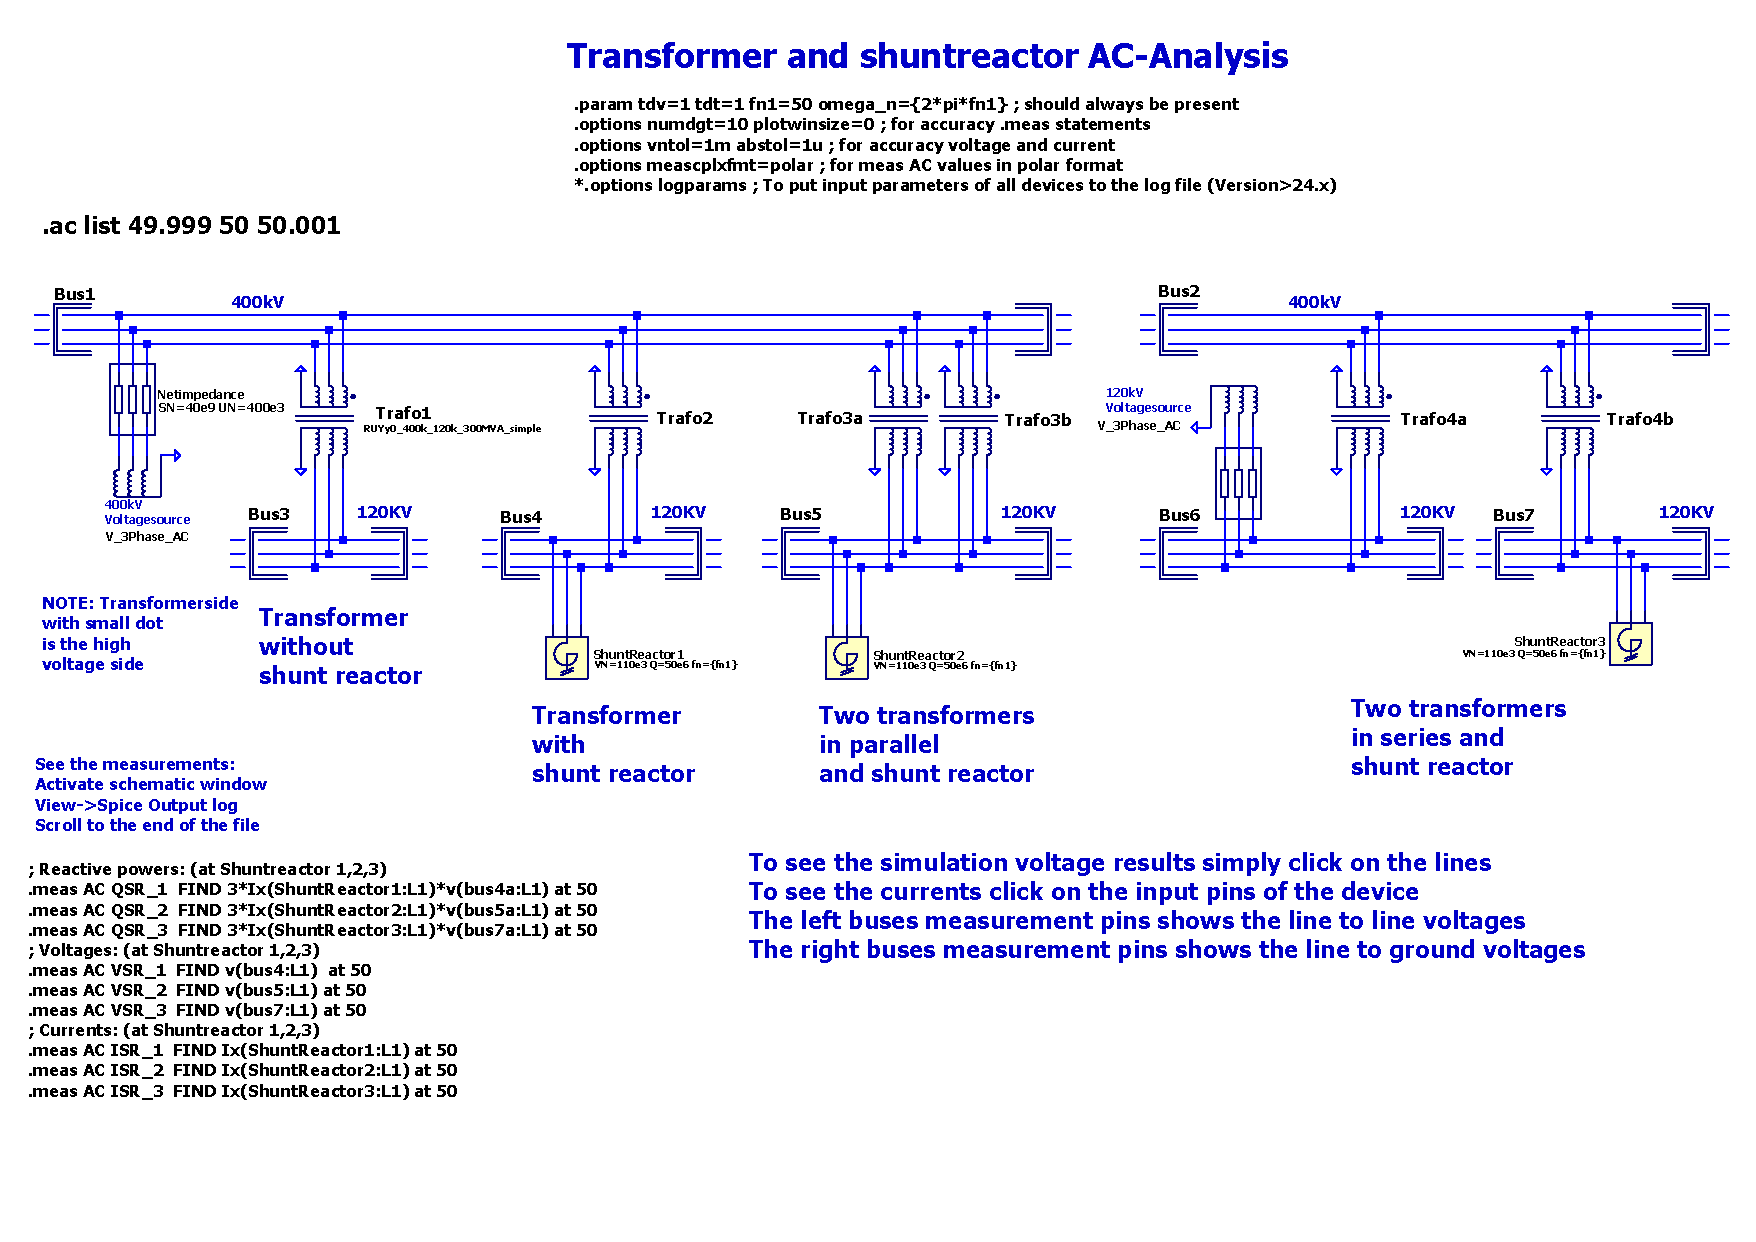
\includegraphics[width=1\textwidth]{figures/01_Transformer und shunt reactor/Transformer_and_shunt_reactor_AC_Schematic.pdf}
	\caption{AC voltages and currents at the shunt reactors.}
	\label{fig:Transformer_and_shunt_reactor_AC_Waveform}
\end{figure}

%\begin{figure}[H]
%	\centering
%	\includegraphics[width=0.99\textwidth]{figures/Transformer_and_shunt_reactor_AC_Schematic}
%	\caption{Schematic for the Transformer and shunt reactor circuit.}
%	\label{fig:Transformer_and_shunt_reactor_AC_Schematic}
%\end{figure}


\begin{figure}[H]
	\centering
	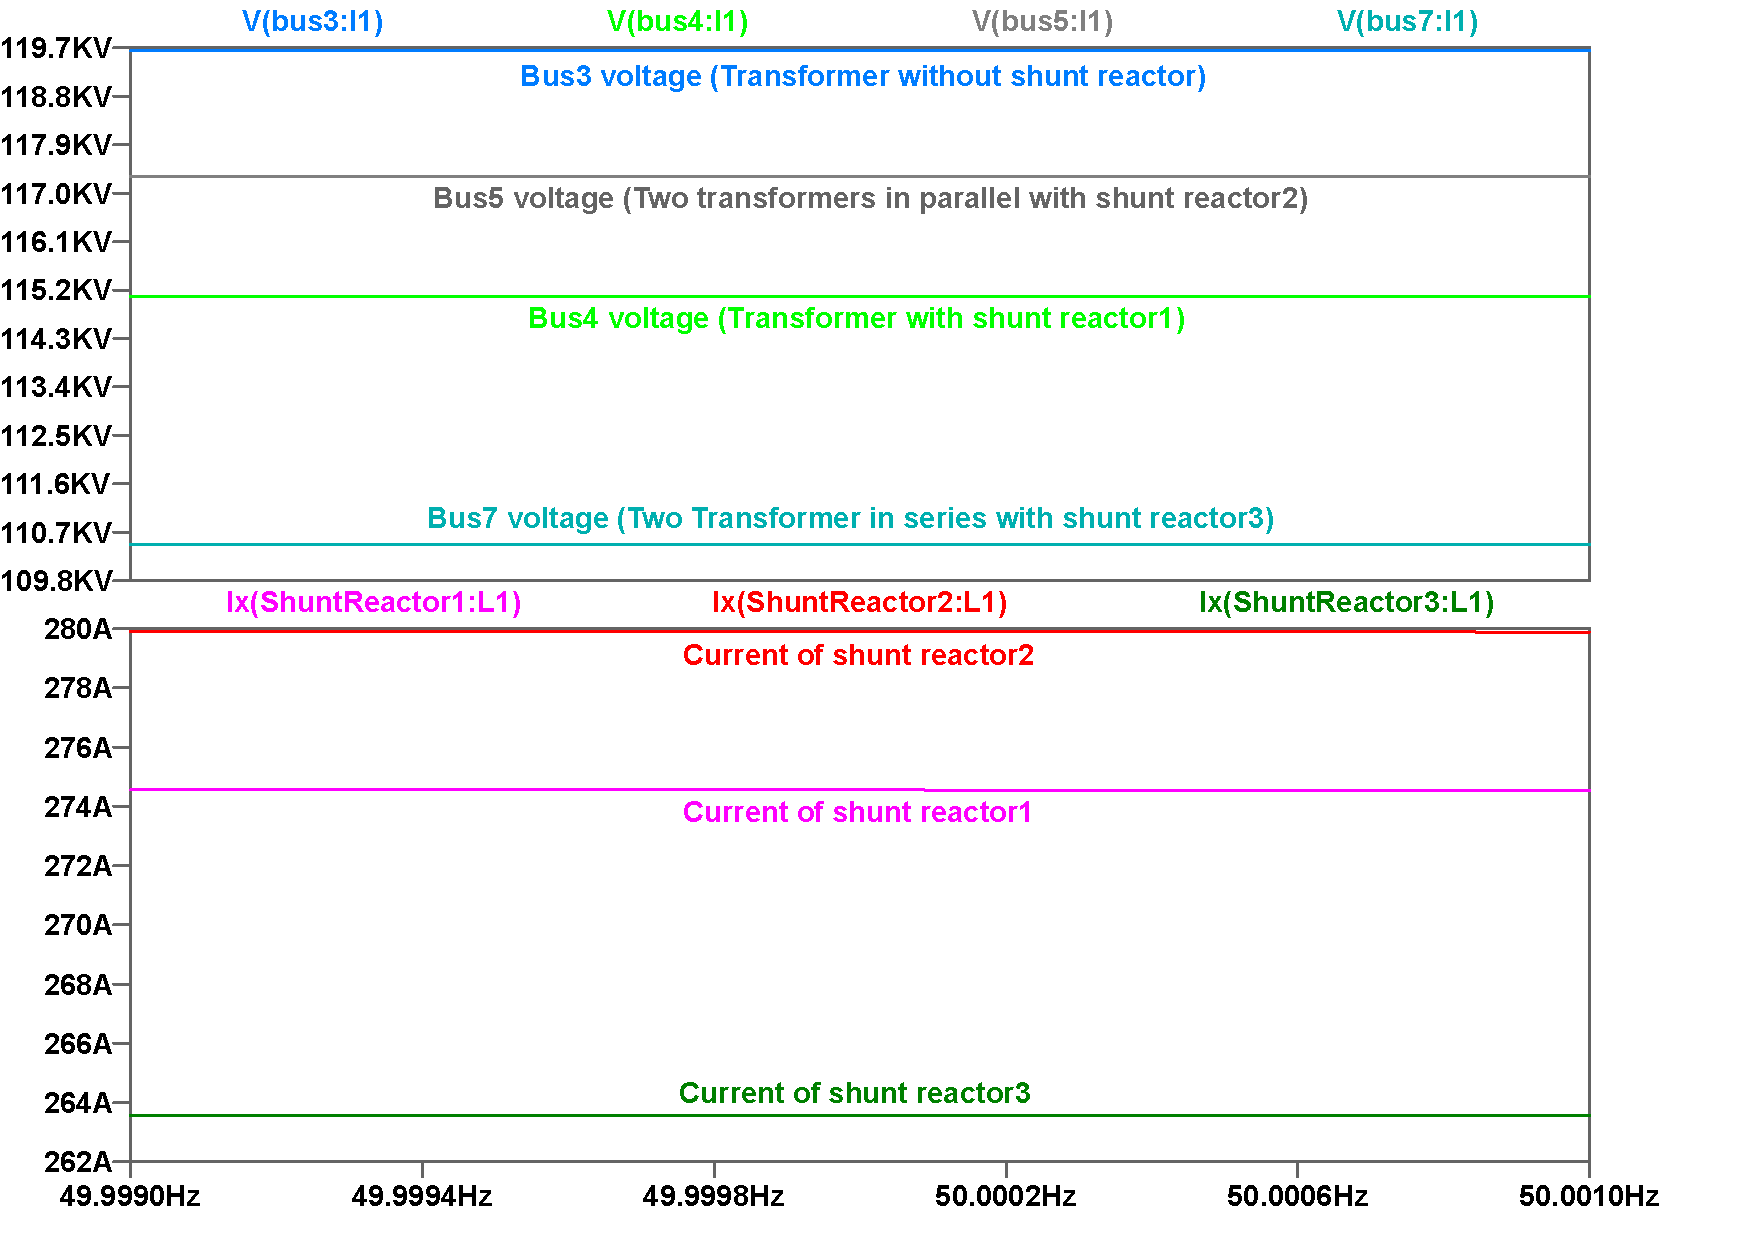
\includegraphics[width=0.90\textwidth]{figures/01_Transformer und shunt reactor/Transformer_and_shunt_reactor_AC_waveform}
	\caption{AC voltages and currents at the shunt reactors.}
	\label{fig:Transformer_and_shunt_reactor_AC_Waveform}
\end{figure}


\begin{chaptersummary}
Shunt reactors are used to regulate the voltage in a power grid. It operates as standalone device or are connected to the tertiary winding of a high voltage transformer.
In this chapter, we have seen that loading a circuit with a shunt reactor reduces the voltage towards the shunt reactor. This voltage reduction occurs whenever a current flow through transformers or the line impedance, which is also highly inductive. As a rule of thumb, inductive reactive power generally flows from the higher voltage level to the lower voltage level. When the transformer is loaded with pure active power, active power always flows from the higher voltage phase angle to the lower voltage angle. 
Real-world example: After energizing a network section via two transformers in series, the voltage is highly volatile. It is best to energize the power district with balanced reactive power. Voltage regulation in the power district should be performed using the regulating transformers and not the shunt reactor. 	
\end{chaptersummary}


\chapter{Short-Circuit Current in the Medium-Voltage Grid}
\label{chap:chapter2}
\index{short-circuit current}
\index{medium-voltage grid}
\index{transformer!parallel operation}

\section{General}
\label{sec:section21}

This example investigates the short-circuit current close to a substation when
two medium-voltage transformers, each rated at \SI{40}{\mega\volt\ampere}, are
operated in parallel. The transient simulation is compared with simple manual
estimates. The influence of an initial load and an additional short-circuit
reactor is then examined, followed by a steady-state AC analysis.

\section{Circuit Design}
\label{sec:section22}

We open the circuit-file \texttt{Shortcircuit\_Current.asc}. This example introduces the line device. Depending on the selected model, this device represents either an overhead line or an underground cable. Here, an oil-insulated underground cable with a conductor cross-section of \SI{500}{\milli\metre\squared} is assumed.

After placing the line element, we opened its attribute window by right-clicking the
symbol. We Double-clicked the \texttt{SpiceModel} field and selected the required
model. We deleted the attributes \texttt{Value2}, \texttt{SpiceLine}, and
\texttt{SpiceLine2}. In the \texttt{Value} attribute, we changed the length
parameter from 1 to 3, corresponding to a line length of \SI{3}{\kilo\metre}.

The high-voltage transformer uses the model
\texttt{RUYYo\_400k\_120k\_300MVA}. Its
\SI{400}{\kilo\volt} side is permanently grounded, whereas the
\SI{120}{\kilo\volt} side is isolated. The tap changer is set to \texttt{L+3}
using

\begin{lstlisting}[style=LTspice]
l_=3 (transformer tap value, pos. sign lower secondary voltage, neg. sign higher secondary voltage)
stproz=1.5 (percentage change in nominal voltage per tap step)
\end{lstlisting}

so that the secondary voltage is approximately \SI{116}{\kilo\volt}.

For the medium-voltage transformers, select the model
\texttt{RUYd5\_110k\_10k\_40MVA}. Their relative short-circuit voltage (ohmic part neglected) is set
to \SI{18}{\percent} with

\begin{lstlisting}[style=LTspice]
ux=0.18 (uk=sqrt(ux*ux+ur*ur))
\end{lstlisting}

The neutral points of the medium-voltage transformers on the \SI{110}{\kilo\volt} side are grounded through a Petersen coil, represented by the additional circuit element \texttt{pet}. The
two \SI{110}{\kilo\volt} lines are assumed to be compensated by this coil. One
cable produces an earth-fault current of approximately \SI{76}{\ampere}; 
This can be verified by deleting all the circuit elements after the line elements.
Now simulate the circuit \texttt{Shortcircuit\_Current.asc} and measure the peak current into the line by dividing the peak current by 1.414 and multiplying the result by three. The earth-fault current
can now be seen in the waveform viewer. % See also at ~\ref{ie:calculation} REFERENCE TO CALCULATION OF EARTH CURRENT   
The Petersen coil is rated at \SI{150}{\ampere} (\textasciitilde 2x76A) and is connected to both
transformer neutral points. When measuring the Petersen-coil voltage, you can observe a slowly varying amplitude during the settling process. This is because of the slight undercompensation or overcompensation of the Petersen coil

To obtain a realistic voltage across the Petersen coil, the phase-1
capacitance of line 1 is changed from \SI{400}{\nano\farad} to
\SI{401}{\nano\farad}. This introduces a small asymmetry. A Petersen coil is not modelled in this example on the \SI{10}{\kilo\volt} side. Because the transformer secondary
is delta-connected, a neutral point would be created with the grounding-transformer element
\texttt{Trafo\_gnd} element, connected to the transformer secondary terminals.

The earth-fault element \texttt{fault\_earth} is also introduced. It is
switched on at \SI{500}{\milli\second} by setting

\begin{lstlisting}[style=LTspice]
t_start=500m
\end{lstlisting}

\begin{remark}{Model asymmetry}{rem:remark21}
The deliberate \SI{1}{\nano\farad} capacitance difference prevents a perfectly
symmetrical zero-voltage condition across the Petersen coil.
\end{remark}

\section{Transient Simulation}
\label{sec:section23}

\subsection{Before the Fault}
The Petersen coil does not play a significant role in this short-circuit example.
We now start the simulation.
Before the fault, the line-to-line voltage is approximately
\SI{116}{\kilo\volt}and the line currents are predominantly capacitive charging
currents with a peak value of approximately \SI{35}{\ampere}.

\subsection{Fault Inception}
At fault inception, the short-circuit current at the fault position reaches a maximum instantaneous peak
value of approximately \SI{53}{\kilo\ampere}. The \SI{116}{\kilo\volt} voltage decreases to
approximately \SI{99}{\kilo\volt}. The RMS voltage can be checked at the measurement pins of bus4, the bus element on the right side

\begin{remark}{Output of measurement values}{rem:remark22}
The values calculated with .meas statements can be viewed in the SPICE output log. Activate the schematic window, select \texttt{View → SPICE Output Log}, and scroll to the end.
\end{remark}

\subsection{Settled Fault Current}
\label{sec:scc-simulation}
After the transient components have largely decayed---approximately
\SI{200}{\milli\second} after fault inception---the steady state short-circuit current is
approximately \SI{30}{\kilo\ampere} peak, or \SI{22}{\kilo\ampere} RMS. The
voltage on the \SI{400}{\kilo\volt} side is approximately
\SI{396}{\kilo\volt}.

\begin{result}{Transient simulation results}{result21}
The principal simulated values are a first peak of approximately
\SI{53}{\kilo\ampere} and a settled RMS short-circuit current of approximately
\SI{22}{\kilo\ampere}.
\end{result}

\section{Estimating the Steady-State Short-Circuit Current}
\label{sec:section24}

The RMS value of the steady-state short-circuit current can be estimated from
the transformer rating and relative short-circuit voltage. The rated current
on the medium-voltage side of one transformer is

\begin{calculation}{Short-circuit current estimate}{Calculation21}
\begin{align}
I_{N}
  &= \frac{S_N}{\sqrt{3}\,U_N} \\
  &= \frac{\SI{40}{\mega\volt\ampere}}
          {\sqrt{3}\cdot\SI{10.6}{\kilo\volt}} \\
  &\approx \SI{2.18}{\kilo\ampere}.
\end{align}

For a relative short-circuit voltage of $u_k=0.18$, the approximate
short-circuit-current factor is

\begin{equation}
\frac{1}{u_k}=\frac{1}{0.18}\approx 5.5.
\end{equation}

Thus, one transformer contributes approximately

\begin{equation}
I_{k,1}\approx 5.5\cdot\SI{2.18}{\kilo\ampere}
          =\SI{12}{\kilo\ampere}.
\end{equation}

For two identical transformers in parallel,

\begin{equation}
I_{k,2}\approx 2I_{k,1}=\SI{24}{\kilo\ampere}.
\end{equation}

This value applies at the nominal primary voltage of \SI{110}{\kilo\volt}.
Because the 110kV operating voltage decreases to approximately
\SI{100}{\kilo\volt}, the corrected estimate is

\begin{equation}
I_k\approx \frac{100}{110}\cdot\SI{24}{\kilo\ampere}
    =\boxed{\SI{21.8}{\kilo\ampere}}.
\end{equation}
\end{calculation}

Considering the simplifying assumptions, the manual estimate of approximately
\SI{21.8}{\kilo\ampere} agrees well with the simulated RMS value of
approximately \SI{22}{\kilo\ampere} in section \ref{sec:scc-simulation}.

\section{Short-Circuit Current with Initial Load}
\label{sec:section25}
Open the file \texttt{Shortcircuit\_Current\_with\_initial\_load.asc}.
A shunt reactor is used as the initial load. It reduces the operating voltage
and therefore also reduces the short-circuit current. The first current peak is
slightly lower, and the settled RMS current (Peak-value/1.414) is approximately
\SI{20.8}{\kilo\ampere}.

\section{Short-Circuit Reactor}
\label{sec:section26}
\index{short-circuit reactor}
Load file  \texttt{Shortcircuit\_Current\_with\_scr.asc}.
An additional short-circuit reactor, denoted by \texttt{scr} in the model, is
now introduced. For strongly inductive currents, its reactance causes a larger
voltage drop and limits the short-circuit current. During normal operation with
predominantly resistive current, the voltage drop across the reactor is much
smaller. The parameter \texttt{delta\_un=5\%} specifies the percentage voltage
drop at rated, purely inductive current.

With this reactor, the first transient current peak is reduced to approximately
\SI{11}{\kilo\ampere}, and the settled RMS short-circuit current is
approximately \SI{4.4}{\kilo\ampere}. The voltages are approximately
\SI{113.5}{\kilo\volt} on the \SI{110}{\kilo\volt} level,
\SI{399.8}{\kilo\volt} on the \SI{400}{\kilo\volt} level and
\SI{9}{\kilo\volt} on the \SI{10}{\kilo\volt} level.
\subsection{Manual Calculation}

For a reactor rated at $U_N=\SI{10}{\kilo\volt}$ and
$I_N=\SI{250}{\ampere}$ and with \texttt{delta\_un=5\%} , the nominal three-phase apparent power is

\begin{calculation}{Fault current behind the reactor}{calculation22}
\begin{align}
S_D
  &= \sqrt{3}\,U_N I_N \\
  &= \sqrt{3}\cdot\SI{10}{\kilo\volt}
     \cdot\SI{250}{\ampere} \\
  &\approx \SI{4.33}{\mega\volt\ampere}.
\end{align}

With the specified relative inductive voltage drop, the reactor impedance is

\begin{equation}
X_D=\frac{\Delta u_N}{100}\frac{U_N^2}{S_D}
   \approx\SI{1.15}{\ohm}.
\end{equation}

The maximum RMS fault current immediately behind the reactor is therefore

\begin{align}
I_{kD}
  &= \frac{U_N}{\sqrt{3}\,X_D} \\
  &= \frac{\SI{10}{\kilo\volt}}
          {\sqrt{3}\cdot\SI{1.15}{\ohm}} \\
  &\approx \SI{5}{\kilo\ampere}.
\end{align}

This assumes a perfectly stiff operating voltage. In the example, the voltage
drops from \SI{10.2}{\kilo\volt} to \SI{8.8}{\kilo\volt}; consequently, the
short-circuit current falls to approximately

\begin{equation}
	I_{kD}\approx\boxed{\SI{4.4}{\kilo\ampere}}.
\end{equation}
\end{calculation}

\section{AC Analysis}
\label{sec:scc-ac-analysis}
Load the file  \texttt{Shortcircuit\_Current\_AC.asc}. 
For the AC analysis, we first replaced the transient voltage-source model with the
corresponding AC source model. Then we adapted the \texttt{.meas} directives, deleted
the fault switch, and we placed the new ground element \texttt{ground} on the
schematic. We added the following option so that complex measurement results are
reported in polar form instead of decibels:

\begin{lstlisting}[style=LTspice]
.options meascplxfmt=polar
\end{lstlisting}

The magnitudes of the voltages and currents agree well with the settled values from
the transient analysis. Directly at the phaseA fault location, however, the
current angle is approximately \ang{120} rather than the initially expected
\ang{-90}. Closer to the voltage source---for example, at the transformer
primary side---the expected current angle of approximately \ang{-90} and voltage
angle of approximately \ang{0} are obtained.

\begin{important}{Effect of transformer vector group}{important21}
The transformer vector group is $\mathrm{Yd5}$, corresponding to a phase shift
of $5\cdot\ang{-30}=\ang{-150}$. For an almost purely inductive fault path, the
current lags the voltage by approximately \ang{-90}. Hence,
\begin{equation}
\varphi_I\approx\ang{-150}+(\ang{-90})=\ang{-240} = \ang{120}.
\end{equation}
Because the fault resistance is assumed to be purely resistive, the current
and the voltage at the fault have approximately the same angle. The theoretical
voltage angle can be checked by removing the ground elements and repeating the
simulation.
\end{important}

\begin{figure}[H]
	\centering
	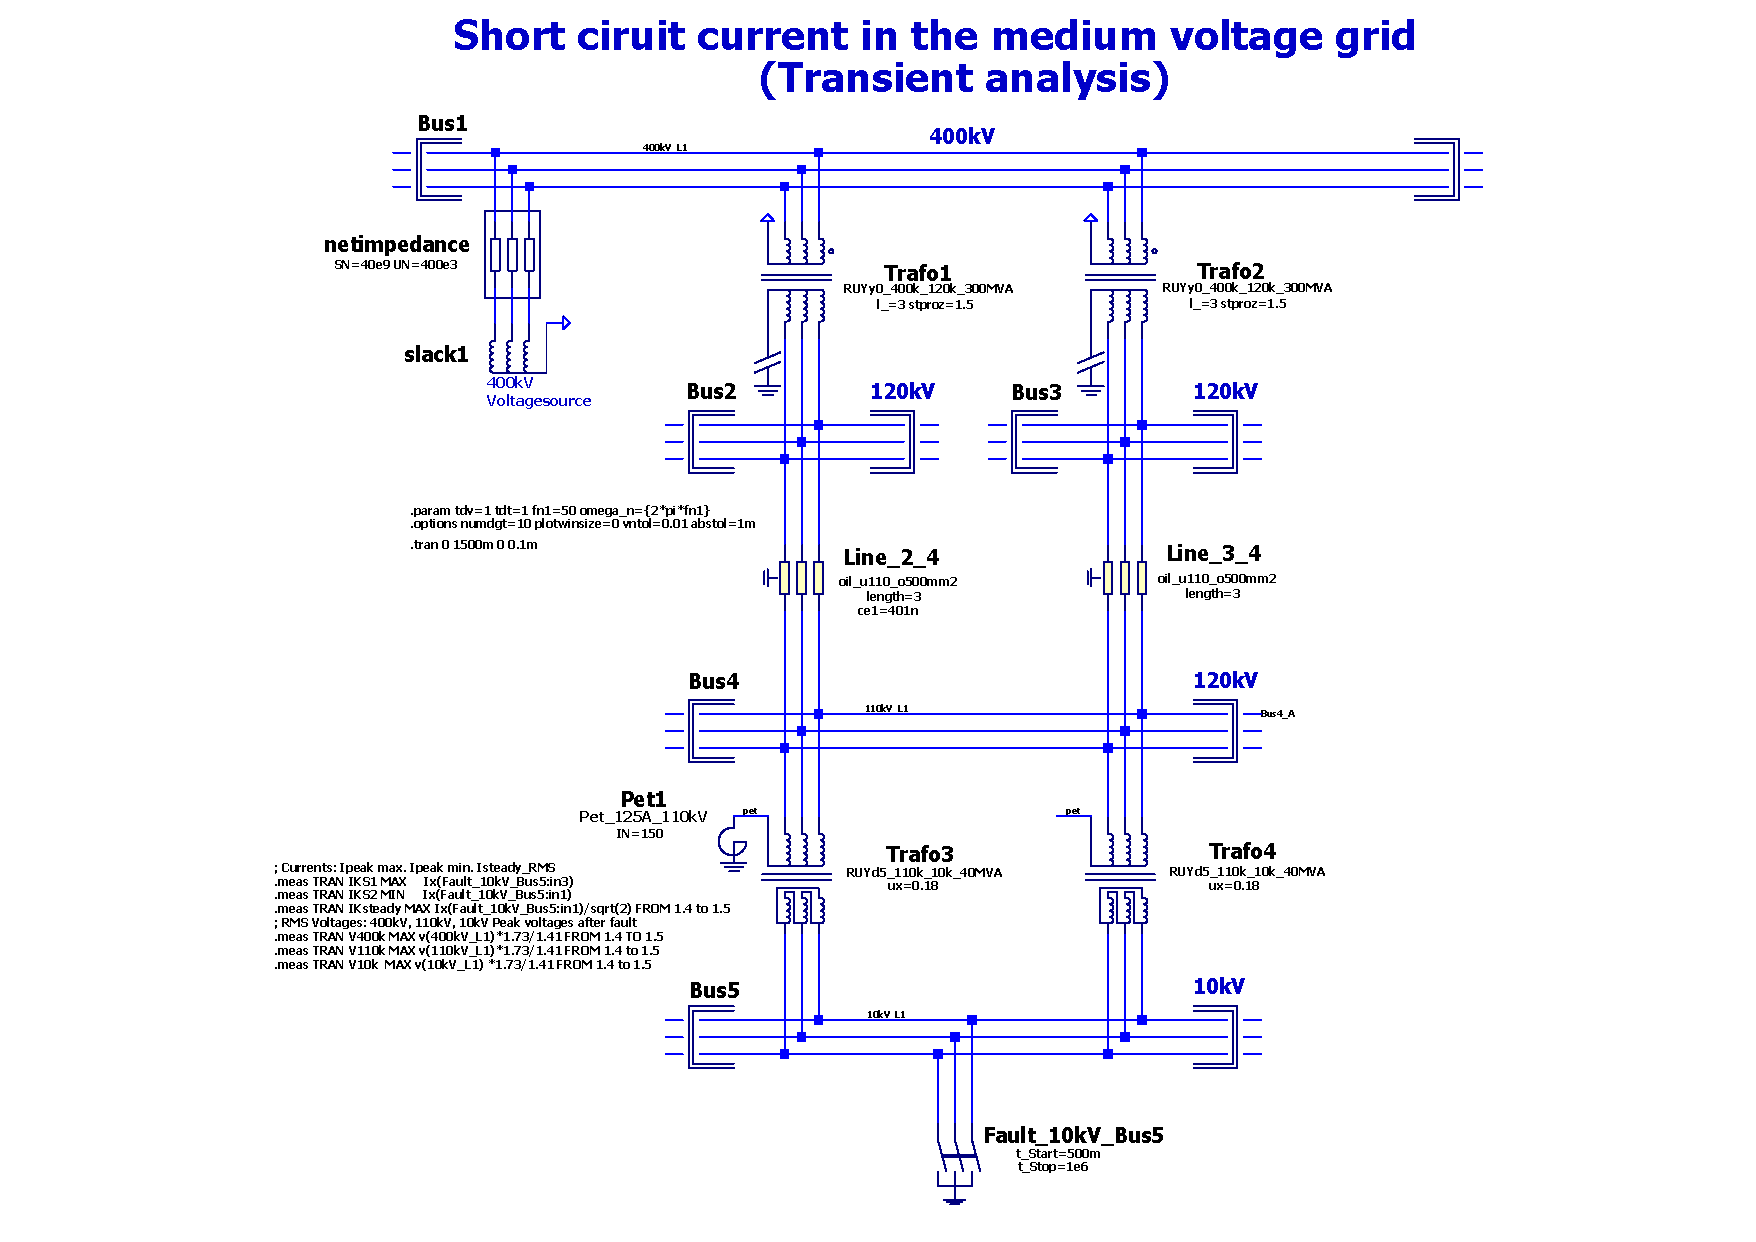
\includegraphics[width=1\textwidth] {figures/02_Shortcircuit in the medium voltage grid/Shortcircuit_Current_Schematic}
	\caption{Shortcircuit in the medium voltage grid - schematic}
	\label{fig:figure21}
\end{figure}

\begin{figure}[H]
	\centering
	\includegraphics[width=0.9\textwidth] {figures/02_Shortcircuit in the medium voltage grid/Shortcircuit_Current_Waveform}
	\caption{Shortcircuit in the medium voltage grid - waveform}
	\label{fig:figure22}
\end{figure}

\begin{figure}[H]
	\centering
	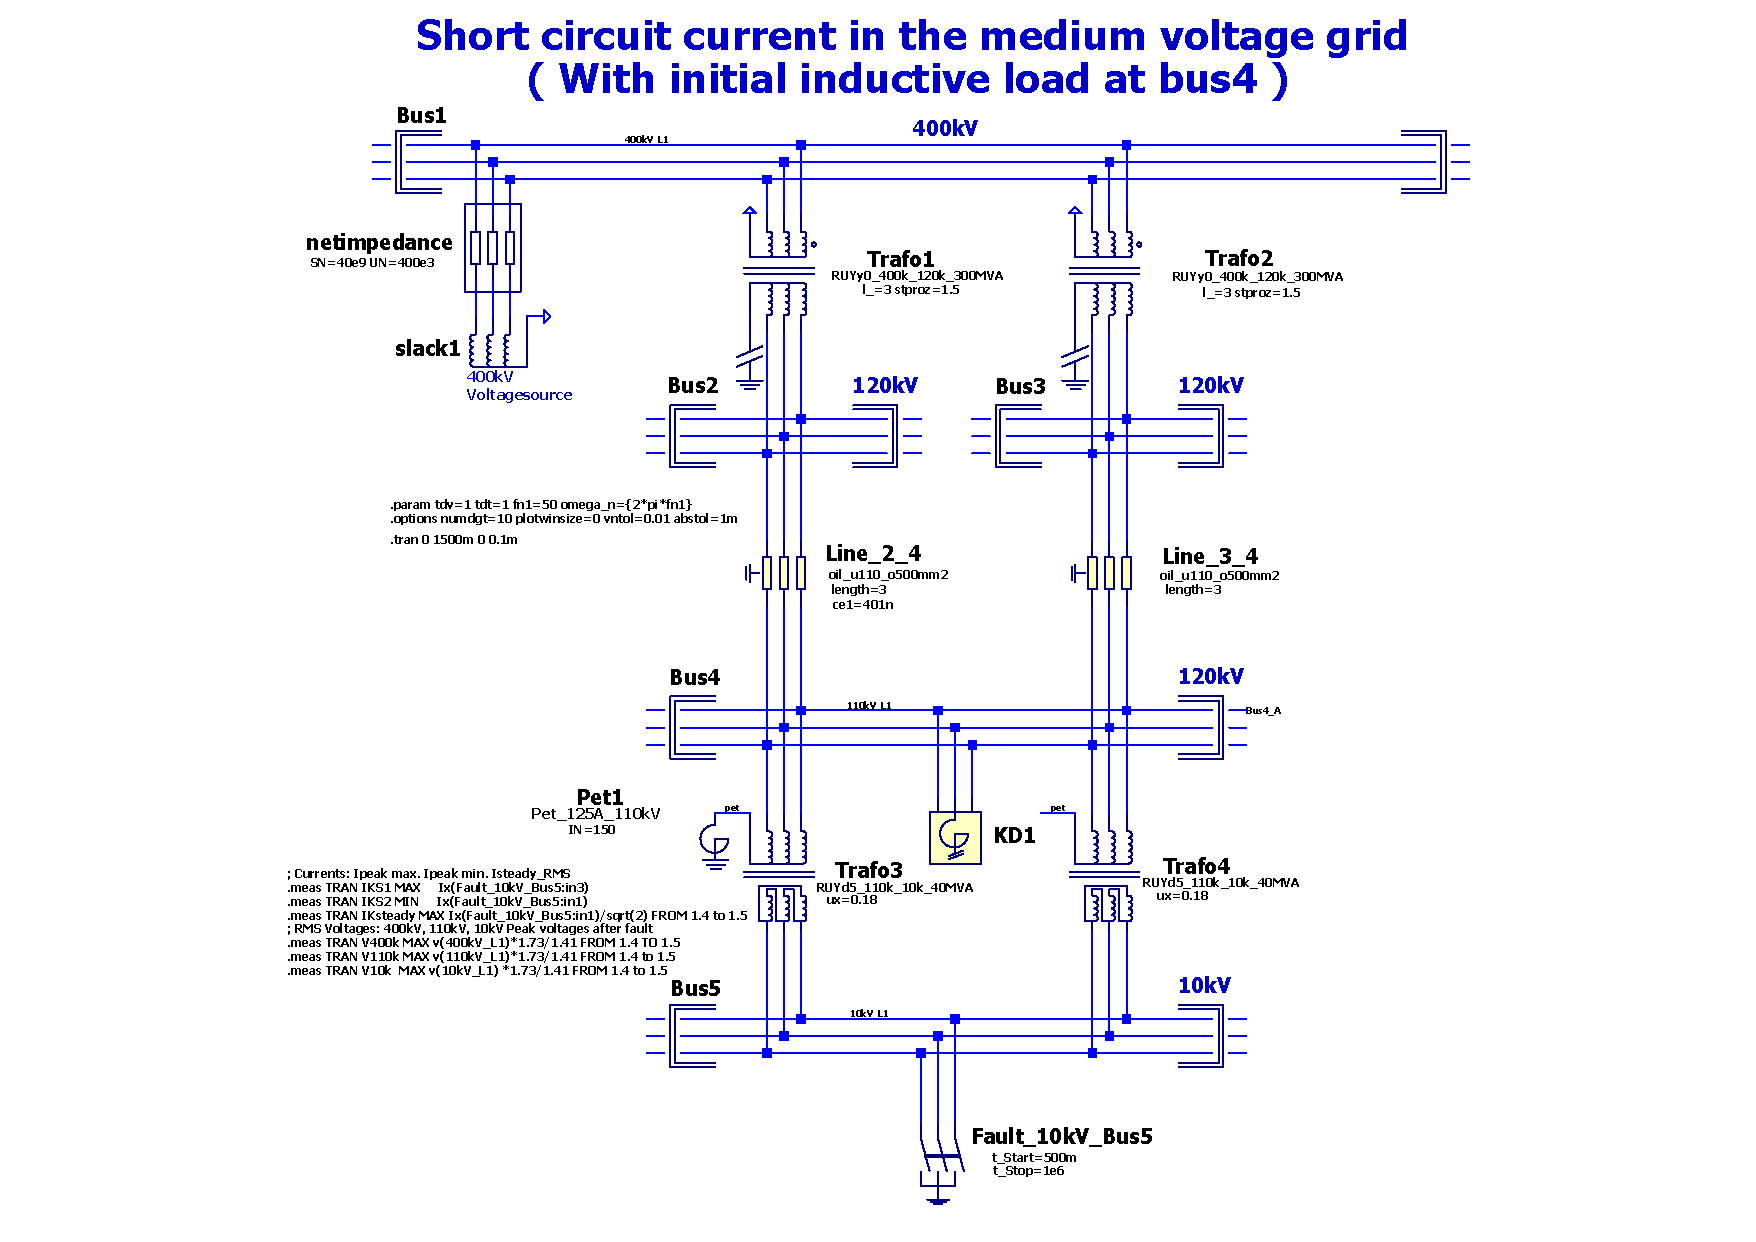
\includegraphics[width=1\textwidth] {figures/02_Shortcircuit in the medium voltage grid/Shortcircuit_Current_with_initial_load_schematic}
	\caption{Shortcircuit in the medium voltage grid with initial load - schematic}
	\label{fig:figure23}
\end{figure}

\begin{figure}[H]
	\centering
	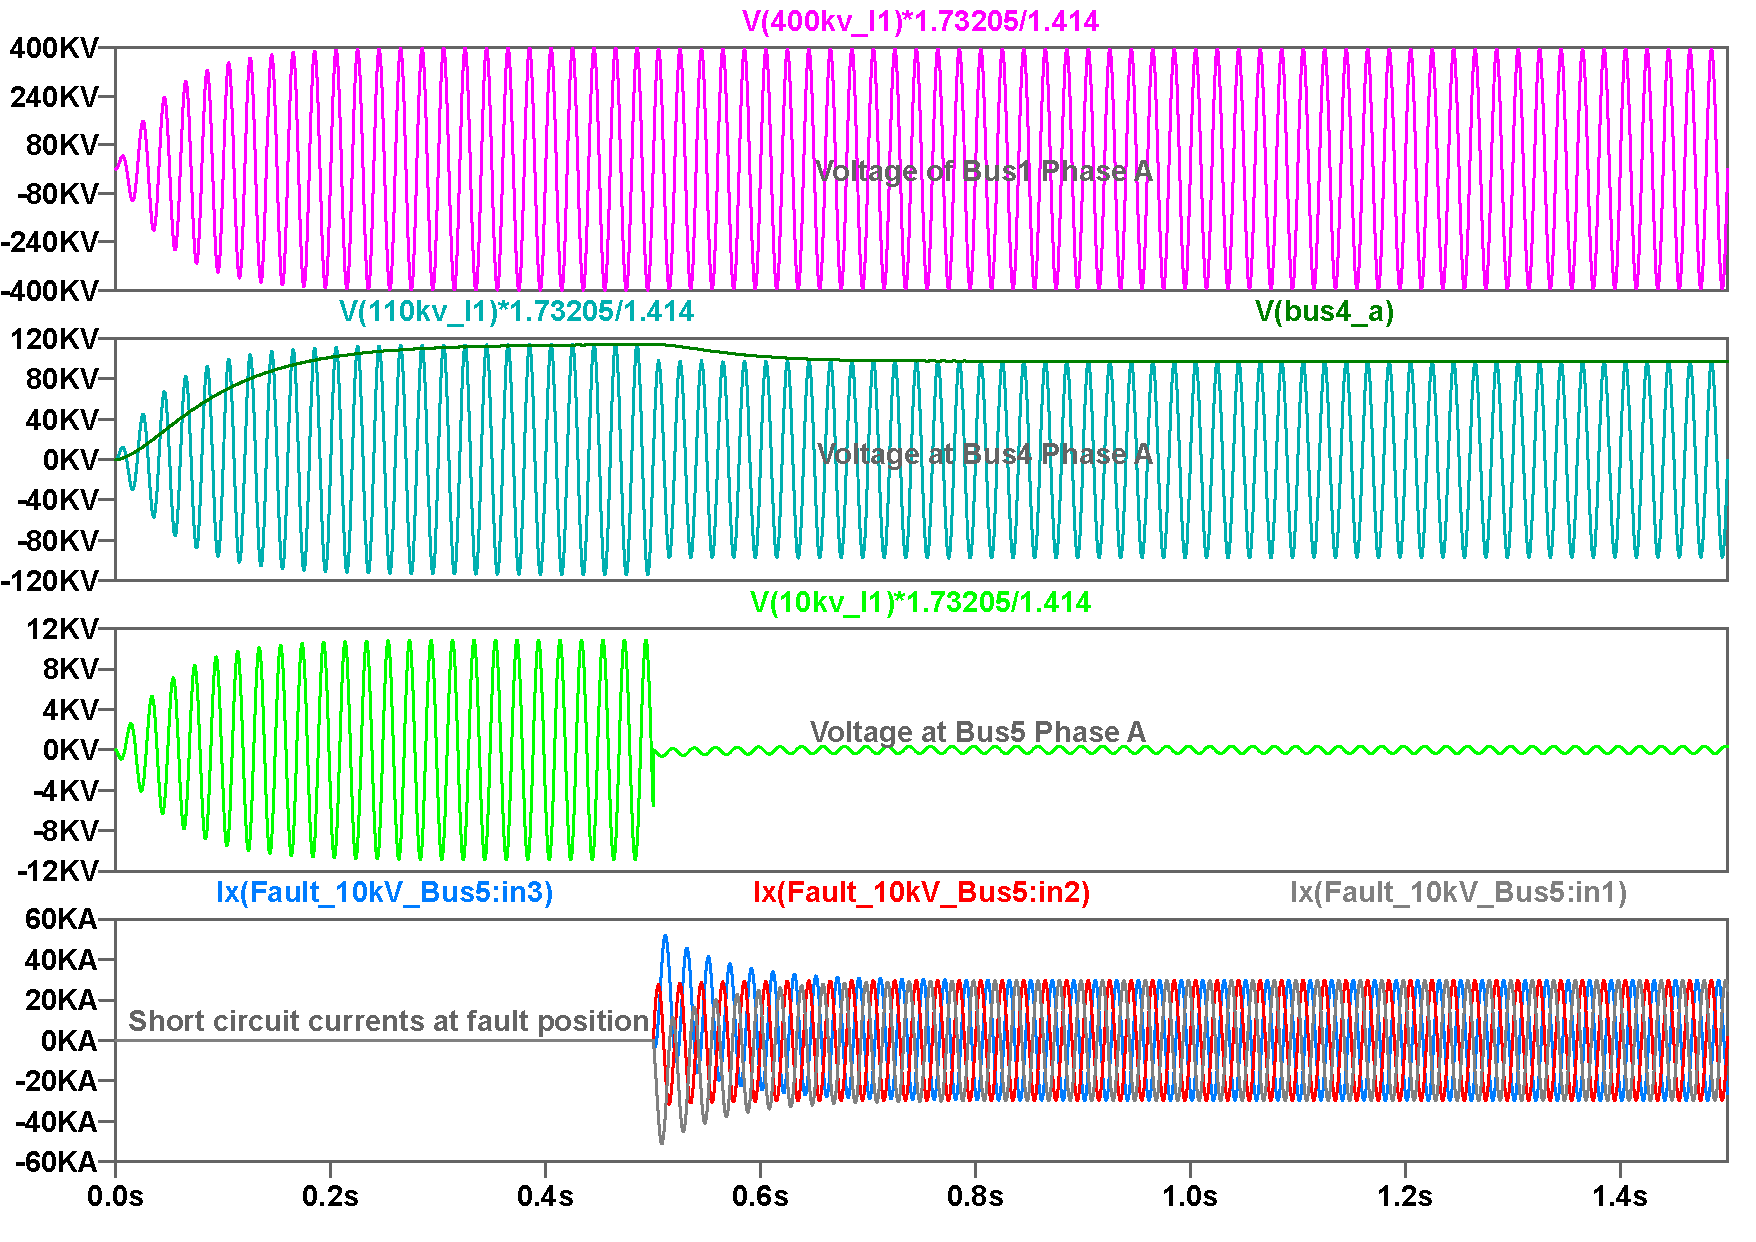
\includegraphics[width=0.9\textwidth] {figures/02_Shortcircuit in the medium voltage grid/Shortcircuit_Current_with_initial_load_waveform}
	\caption{Shortcircuit in the medium voltage grid with initial load - waveform}
	\label{fig:figure24}
\end{figure}

\begin{figure}[H]
	\centering
	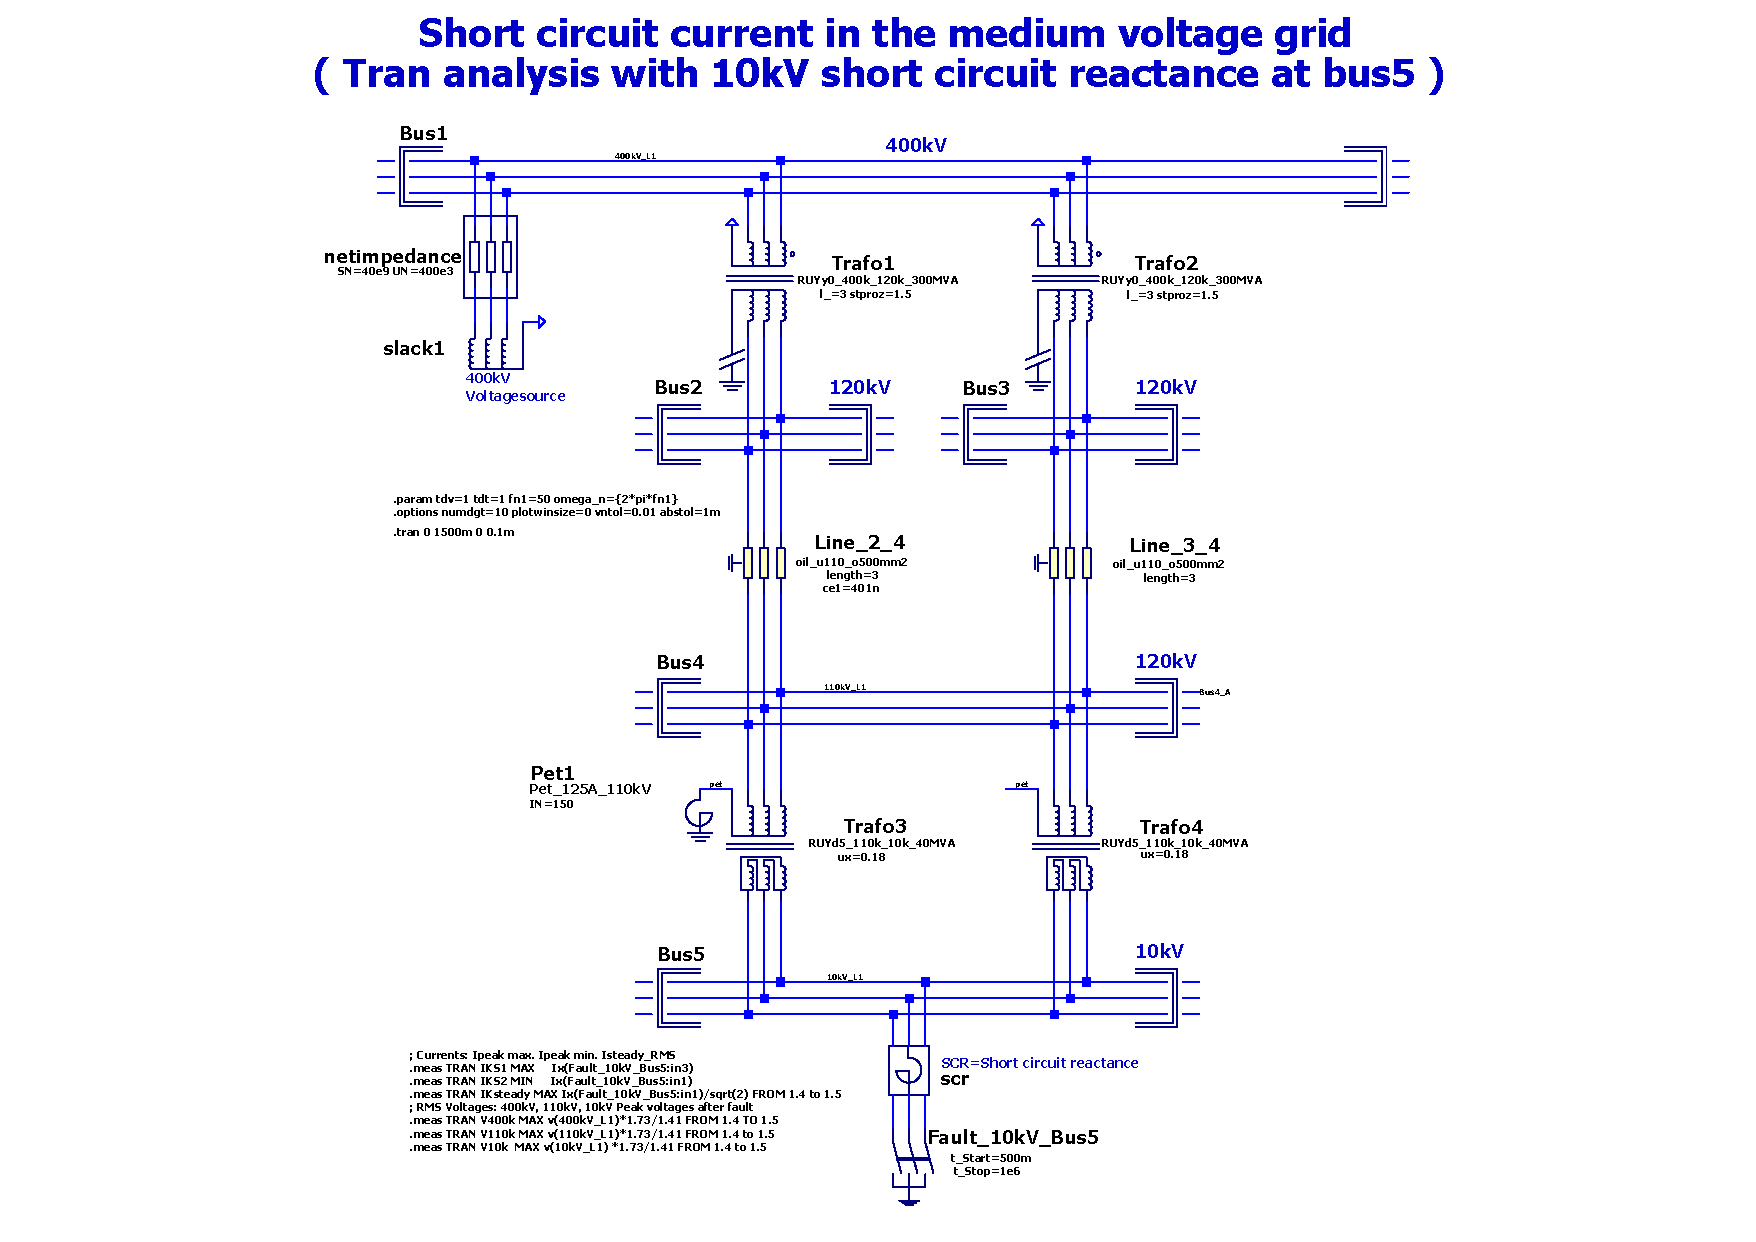
\includegraphics[width=1\textwidth] {figures/02_Shortcircuit in the medium voltage grid/Shortcircuit_Current_with_scr_schematic}
	\caption{Shortcircuit in the medium voltage grid with scr - schematic}
	\label{fig:figure25}
\end{figure}

\begin{figure}[H]
	\centering
	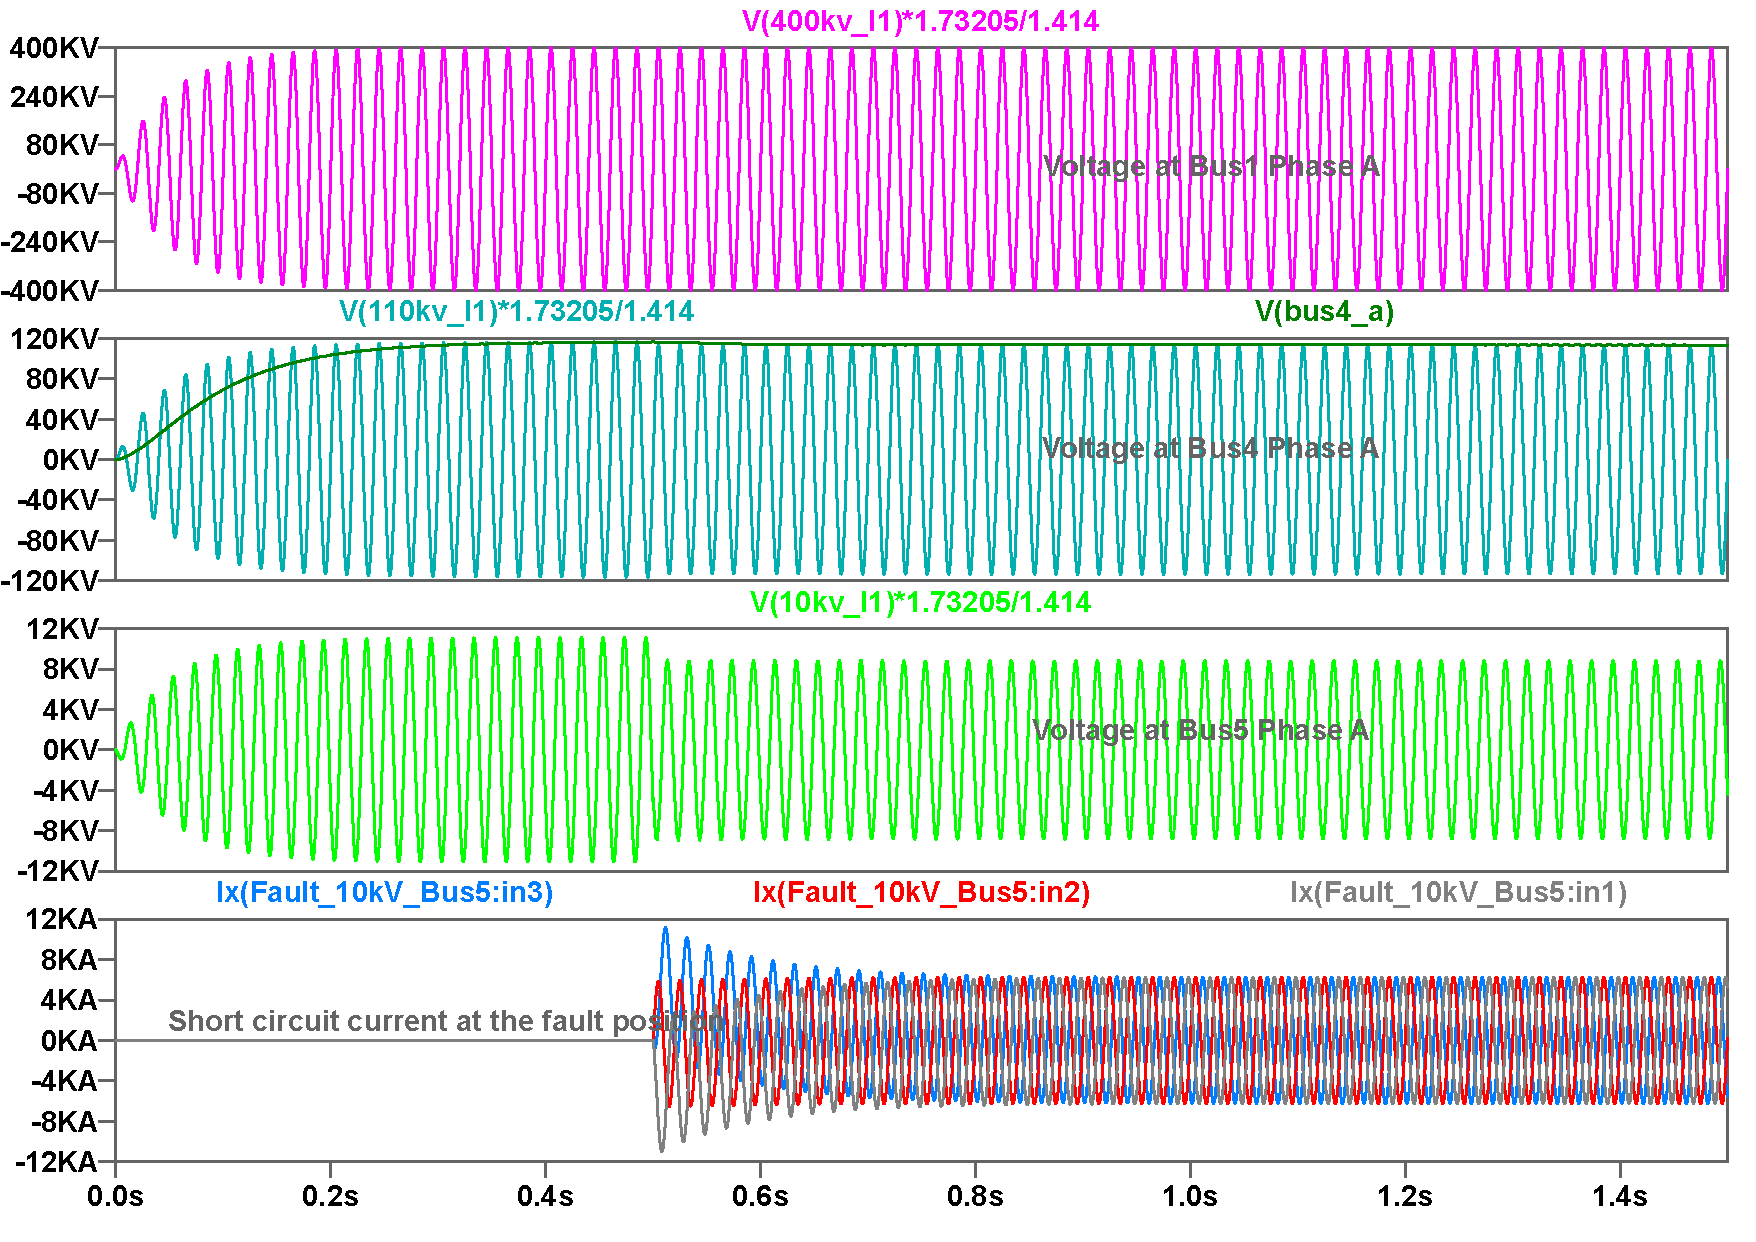
\includegraphics[width=0.9\textwidth] {figures/02_Shortcircuit in the medium voltage grid/Shortcircuit_Current_with_scr_waveform}
	\caption{Shortcircuit in the medium voltage grid with scr - waveform}
	\label{fig:figure26}
\end{figure}

\begin{figure}[H]
	\centering
	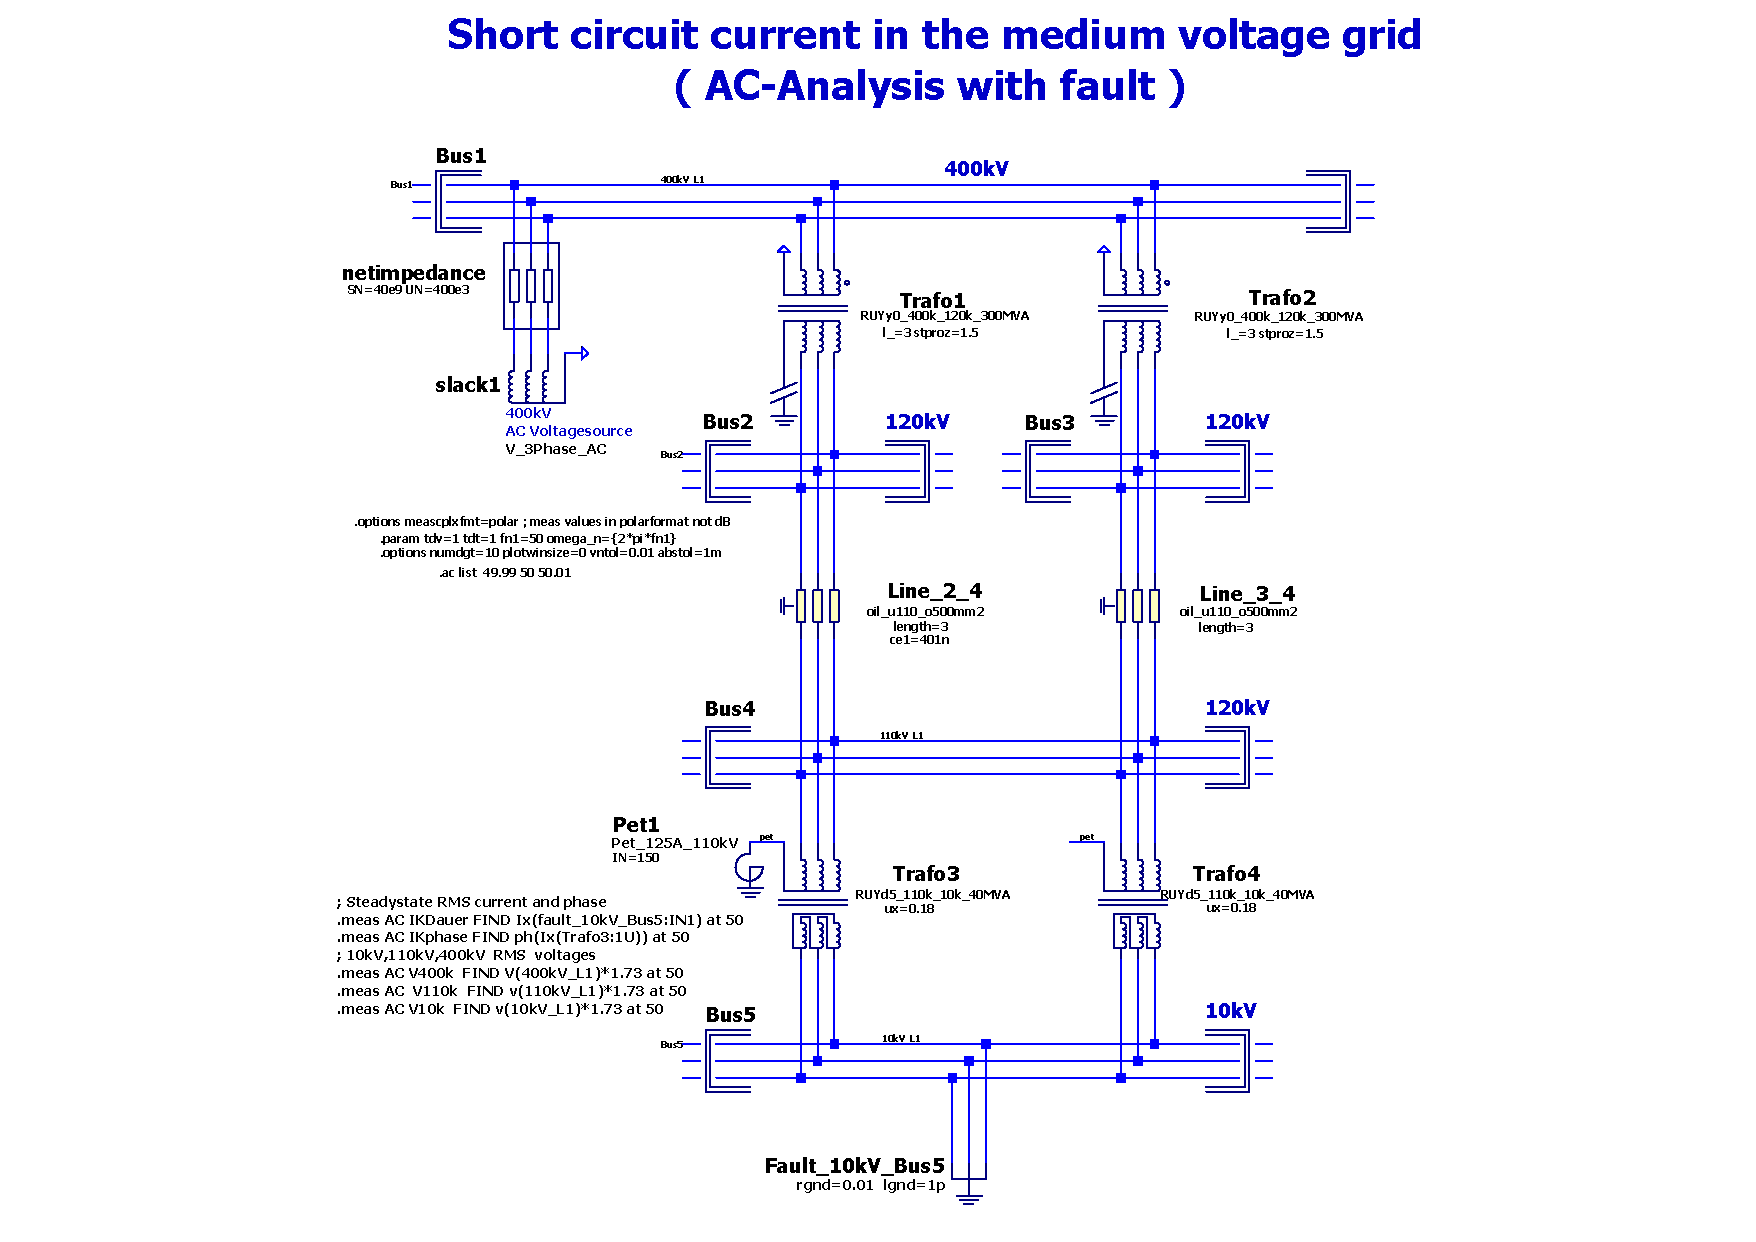
\includegraphics[width=1\textwidth] {figures/02_Shortcircuit in the medium voltage grid/Shortcircuit_Current_AC_schematic}
	\caption{Shortcircuit in the medium voltage grid AC analysis - schematic}
	\label{fig:figure27}
\end{figure}

\begin{figure}[H]
	\centering
	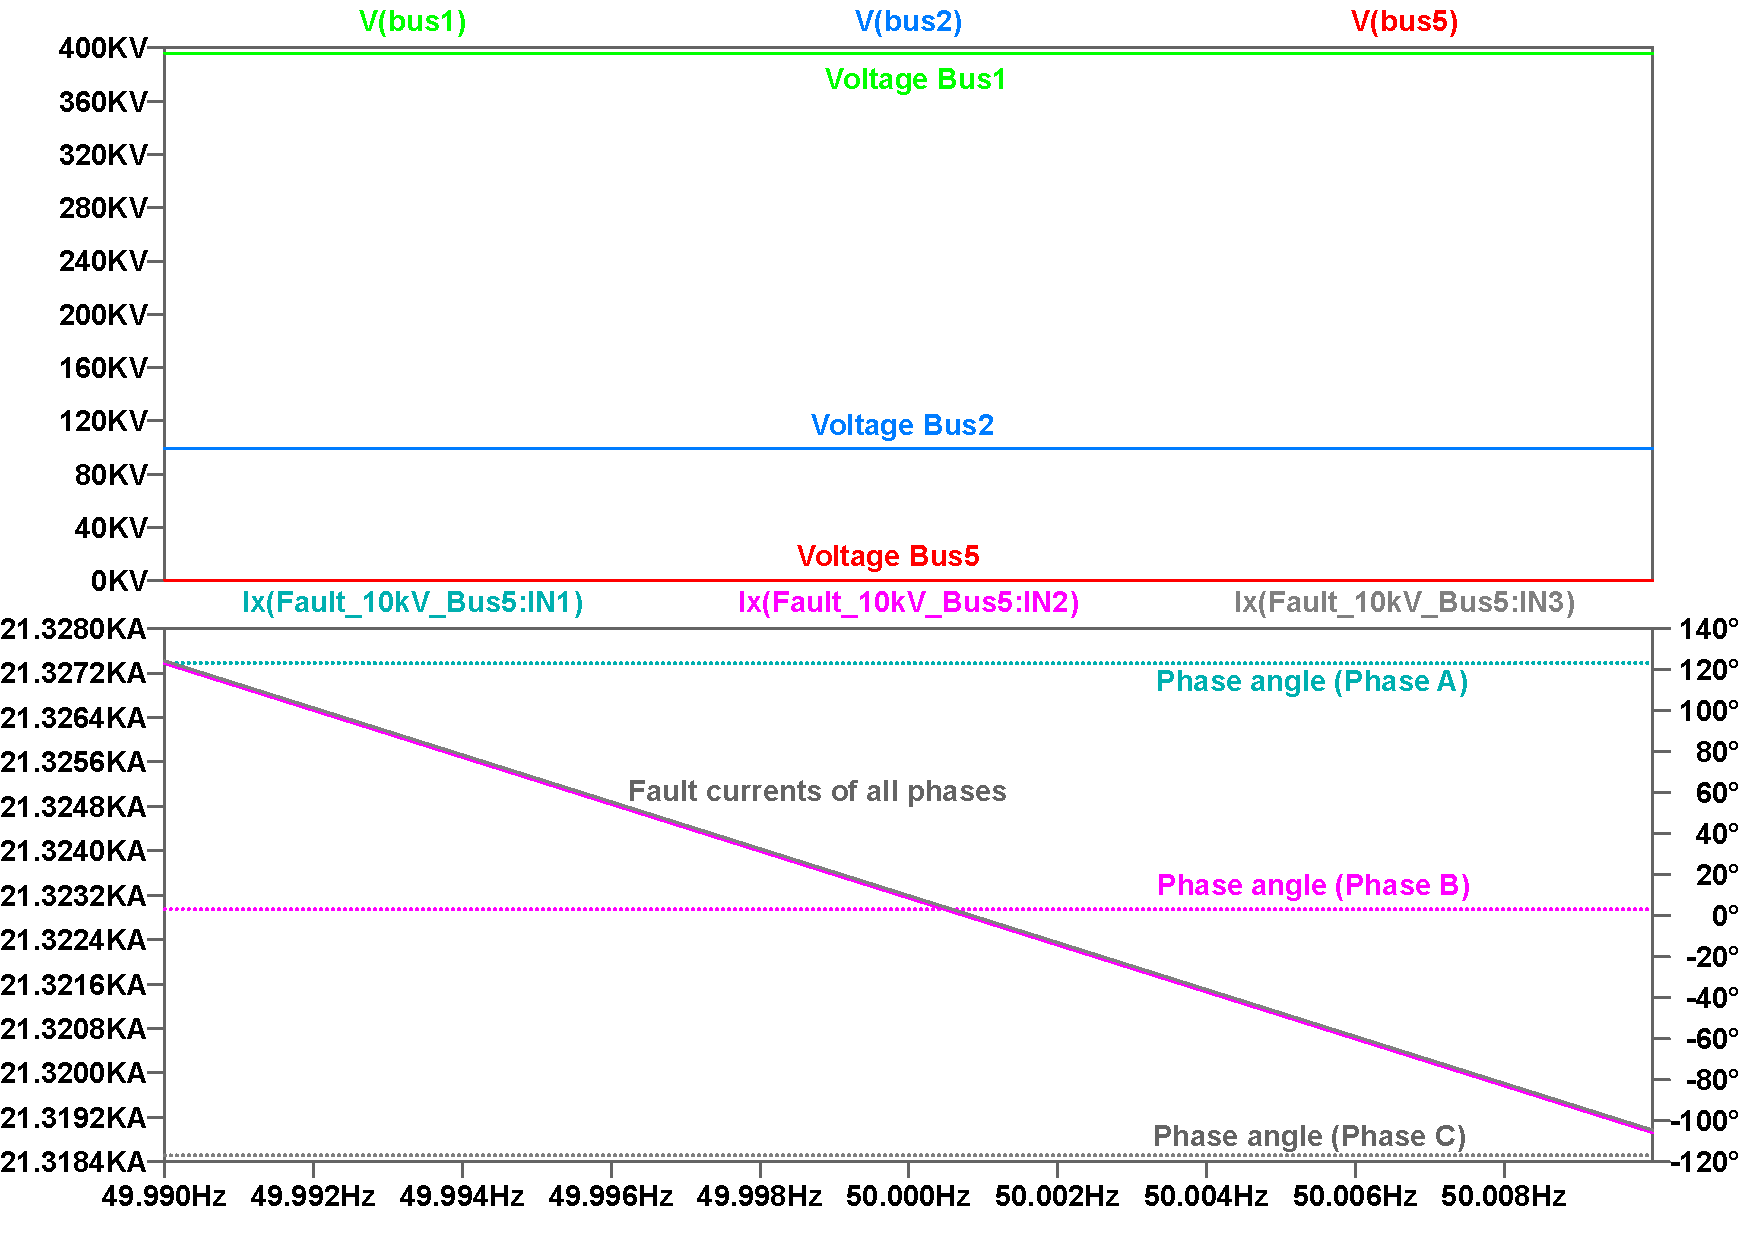
\includegraphics[width=0.9\textwidth] {figures/02_Shortcircuit in the medium voltage grid/Shortcircuit_Current_AC_waveform}
	\caption{Shortcircuit in the medium voltage grid AC analysis - waveform}
	\label{fig:figure28}
\end{figure}

\begin{chaptersummary}
Two \SI{40}{\mega\volt\ampere} medium-voltage transformers operated in
parallel produce a settled short-circuit current of approximately
\SI{22}{\kilo\ampere} RMS in the investigated network. A simple estimate based
on rated current, relative short-circuit voltage, parallel operation, and the
actual operating voltage closely reproduces this result. An initial inductive
load reduces the current slightly, whereas an additional short-circuit reactor
limits it substantially to approximately \SI{4.4}{\kilo\ampere}. The AC
analysis also demonstrates that transformer vector groups must be considered
when interpreting phase angles.
\end{chaptersummary}

\chapter{Initializing Transformers with Residual Flux}
\label{chap:chapter3}
\index{transformer!residual flux}
\index{remanent flux}
\index{inrush current}

\section{General}
\label{sec:section31}
This chapter demonstrates how a transformer model can be initialized with
residual magnetic flux. The examples show how the switching instant and the
polarity of the residual flux determine the maximum core flux and the resulting
magnetizing inrush current.

For an ideal winding, neglecting the winding resistance, the applied voltage
and core flux are related by

\begin{equation}
u(t)=N\frac{\diff\Phi(t)}{\diff t},
\qquad
\Phi(t)=\Phi(0)+\frac{1}{N}\int_0^t u(\tau)\diff\tau.
\label{eq:flux-voltage-integral}
\end{equation}

Consequently, the flux is determined by the time integral of the imposed
voltage and by the initial flux $\Phi(0)$. If a transformer is energized at an
unfavourable point on the voltage waveform, the transient flux can reach twice
its normal steady-state peak. With full residual flux of the same polarity, it
can approach three times the normal peak. Because the core characteristic is
nonlinear, this overfluxing can produce a magnetizing current many times larger
than the normal no-load current.

\begin{important}{Switching instant and residual flux}{Important31}
The initial flux, the voltage phase angle at switching, and the parameter that
applies the initial condition must always be coordinated. A physically
reasonable residual-flux vector in a three-leg core also satisfies approximately
$\Phi_{r0}+\Phi_{s0}+\Phi_{t0}=0$.
\end{important}

\section{Circuit Design}
\label{sec:section32}
For all cases the ltspice file \texttt{Initializing\_Transformers\_with\_residual\_flux.asc} is loaded. 
Four transformer circuits are arranged on the right side of the schematic.
They are supplied at \SI{115}{\kilo\volt}; each transformer is rated
\SI{110}{\kilo\volt}/\SI{10.6}{\kilo\volt}. A switch is placed between each
source and transformer.

The first three circuits are energized at a phase-1 voltage zero crossing and
use different residual-flux settings:

\begin{itemize}
\item no residual flux: \texttt{psi0=0},
\item unfavourable residual flux: \texttt{psi0=1},
\item favourable residual flux: \texttt{psi0=-1}.
\end{itemize}

The fourth circuit is energized at a different point on the voltage waveform
and uses explicitly specified phase residual fluxes. See section 
~\ref{sec:section36}
\begin{remark}{Coordination of initialization time}{remark31}
The transformer parameter \texttt{tpsi0} must match the switch closing time
\texttt{t\_start}. For the first three circuits, use
\begin{lstlisting}[style=LTspice]
t_start=40m  tpsi0=40m
\end{lstlisting}
For the final circuit, use
\begin{lstlisting}[style=LTspice]
t_start=45m  tpsi0=45m
\end{lstlisting}
The \texttt{tpsi0} event rapidly initializes the voltage integrator capacitor
that represents the residual flux.
\end{remark}

\section{Energization at \SI{40}{\milli\second} Without Residual Flux}
\label{sec:section33}
For Trafo1 we set the transformer parameter \texttt{psi0} to zero. The parameter
\texttt{tpsi0} may either be set to \SI{40}{\milli\second} or placed well
outside the simulation interval, for example at \SI{1000}{\second}, because no initial flux has to be applied to Transformer1.

At \SI{40}{\milli\second}, the trace v(phaseA1) voltage starts at zero and initially
becomes positive. Its integral therefore acquires a unidirectional offset. At
\SI{10}{\milli\second} after energization, the phase-1 flux reaches
approximately twice the normal steady-state peak, and the magnetizing current
rises accordingly.

The three phase fluxes can be displayed in the LTspice waveform viewer with

\begin{lstlisting}[style=LTspice]
V(Trafo1:u:_w1:phi)
V(Trafo1:v:_w1:phi)
V(Trafo1:w:_w1:phi)
\end{lstlisting}

Both flux and current decay slowly because a large power transformer has a high
magnetizing inductance and a long electrical time constant. Increasing the
resistance of the source impedance accelerates the decay. This can be examined
with $R=\SI{10}{\ohm}$, \SI{100}{\ohm}, and \SI{1000}{\ohm}.

The rated primary current is approximately \SI{210}{\ampere} RMS. In this
case, the peak magnetizing current is approximately \SI{70}{\ampere}, or about
\SI{50}{\ampere} RMS, and therefore remains below the rated current.

The steady-state peak flux V(trafo1:u:\_w1:phi) is \SI{0.3}{\weber} and the initial flux is 2*\SI{0.3}{\weber}.


\begin{calculation}{Rated steady-state flux}{calculation31} % hier ohne calc: für ref auf gesamte Box 
	% unten mit Calculation~\ref{calc:rated-flux} und 2x compilieren !!!
\begin{align}
\widehat{\Phi}_N
  &=\frac{\sqrt{2}\,U_{\mathrm{ph}}}{\omega N_1}
   =\frac{\sqrt{2}\,U_{\mathrm{LL}}}
          {\sqrt{3}\,\omega N_1}.
          %\label{eq:rated-flux} % für einzelne ref auf formel -> Equation~\eqref{eq:rated-flux}
\end{align}

With $U_{\mathrm{LL}}=\SI{115}{\kilo\volt}$,
$\omega=2\pi\cdot\SI{50}{\hertz}$, and the toolbox default
$N_1=1000$, this gives

\begin{align}
\widehat{\Phi}_N
  &=\frac{\sqrt{2}\cdot\SI{115}{\kilo\volt}}
          {\sqrt{3}\cdot 2\pi\cdot\SI{50}{\hertz}\cdot1000}
    \approx\boxed{\SI{0.299}{\weber}}.
\end{align}
\end{calculation}

\begin{remark}{Line-to-line and phase voltage}{remark32}
For a star-connected three-phase winding, use the phase voltage $U_{ph} = U_{LL}/√3$ and include the RMS-to-peak factor √2 when calculating the peak flux. It is particularly interesting that the magnetic flux depends only on voltage !!! 
\end{remark}

\section{Energization at \SI{40}{\milli\second} with Unfavourable Residual Flux}
\label{sec:section34}

We set \texttt{psi0=1} for Trafo1 . Unless the individual phase parameters are overridden,
the model initializes the phase residual-flux values to

\begin{equation}
(\psi_{r0},\psi_{s0},\psi_{t0})=(1,-0.5,-0.5)\;\text{p.u.}
\end{equation}

Phase 1 therefore starts with full positive residual flux, while phases 2 and
3 start with half the negative value. Since the phase-1 voltage becomes
positive immediately after the switch closes, its integral adds to the
positive residual flux. Approximately \SI{10}{\milli\second} later, the flux
reaches approximately three times the steady-state peak.

The phase-1 current reaches approximately \SI{900}{\ampere} peak. The corresponding RMS value can be calculated in LTspice by zooming in from 40 ms to 60 ms and then left-clicking on the trace name Ix(Trafo2:1U) using the Control button. A pop-up window will then appear, and you can read the RMS value as 380A. This is the procedure to follow if the waveform is not sinusoidal.
The inrush current decays comparatively quickly because the high current
increases the effective damping of the transient.

The corresponding flux traces are

\begin{lstlisting}[style=LTspice]
V(Trafo2:u:_w1:phi)
V(Trafo2:v:_w1:phi)
V(Trafo2:w:_w1:phi)
\end{lstlisting}

The residual-flux values are visible as the initial values at the switching
instant.

\section{Energization at \SI{40}{\milli\second} with Favourable Residual Flux}
\label{sec:section35}

Set \texttt{psi0=-1}. The internal phase residual-flux vector becomes

\begin{equation}
(\psi_{r0},\psi_{s0},\psi_{t0})=(-1,0.5,0.5)\;\text{p.u.}
\end{equation}

The maximum negative phaseA residual flux compensates the positive flux
increment that follows switching at \SI{40}{\milli\second}. Apart from a short
numerical switching spike, the flux moves directly into its steady-state
trajectory and the magnetizing current remains very small.

A similarly smooth startup can be obtained by deleting the switcher and set the Texp parameter of the voltage source to 50ms.

To inspect the small steady-state current in the waveform viewer, manually
limit the current-axis range after the switching spike. The nonlinear
magnetization curve produces a small but visibly distorted current. The phase
fluxes are displayed with ..

\begin{lstlisting}[style=LTspice]
V(Trafo3:u:_w1:phi)
V(Trafo3:v:_w1:phi)
V(Trafo3:w:_w1:phi)
\end{lstlisting}

They are nearly symmetrical with respect to the Y-axis and already settled after energization.

\begin{remark}{Default residual-flux vector}{remark33}
The default vectors $(1,-0.5,-0.5)$ and $(-1,0.5,0.5)$ produce the behaviour
described above only at equivalent points of the \SI{50}{\hertz} waveform,
such as 0, 20, and \SI{40}{\milli\second}. At other switching instants, specify
the individual values with \texttt{psir}, \texttt{psis}, and \texttt{psit}.
\end{remark}

\section{Energization at \SI{45}{\milli\second} with Unfavourable Residual Flux}
\label{sec:section36}

For switching at \SI{45}{\milli\second}, the unfavourable residual-flux vector
differs from the default vector used at the voltage zero crossing. The required
values are as follows:

\begin{lstlisting}[style=LTspice]
psi0=1
psir=0
psis=0.866
psit=-0.866
t_start=45m
tpsi0=45m
\end{lstlisting}

With these settings, the phaseA current is the smallest, whereas the currents
in phases 2 and 3 are the largest. The currents remain high, but their maxima
are lower than in the unfavourable \SI{40}{\milli\second} case seen in section
\ref{sec:section34}.\\
%\vspace{0.5cm}

The phase fluxes can be displayed with ..
\begin{lstlisting}[style=LTspice]
V(Trafo4:u:_w1:phi)
V(Trafo4:v:_w1:phi)
V(Trafo4:w:_w1:phi)
\end{lstlisting}

\begin{figure}[H]
	\centering
	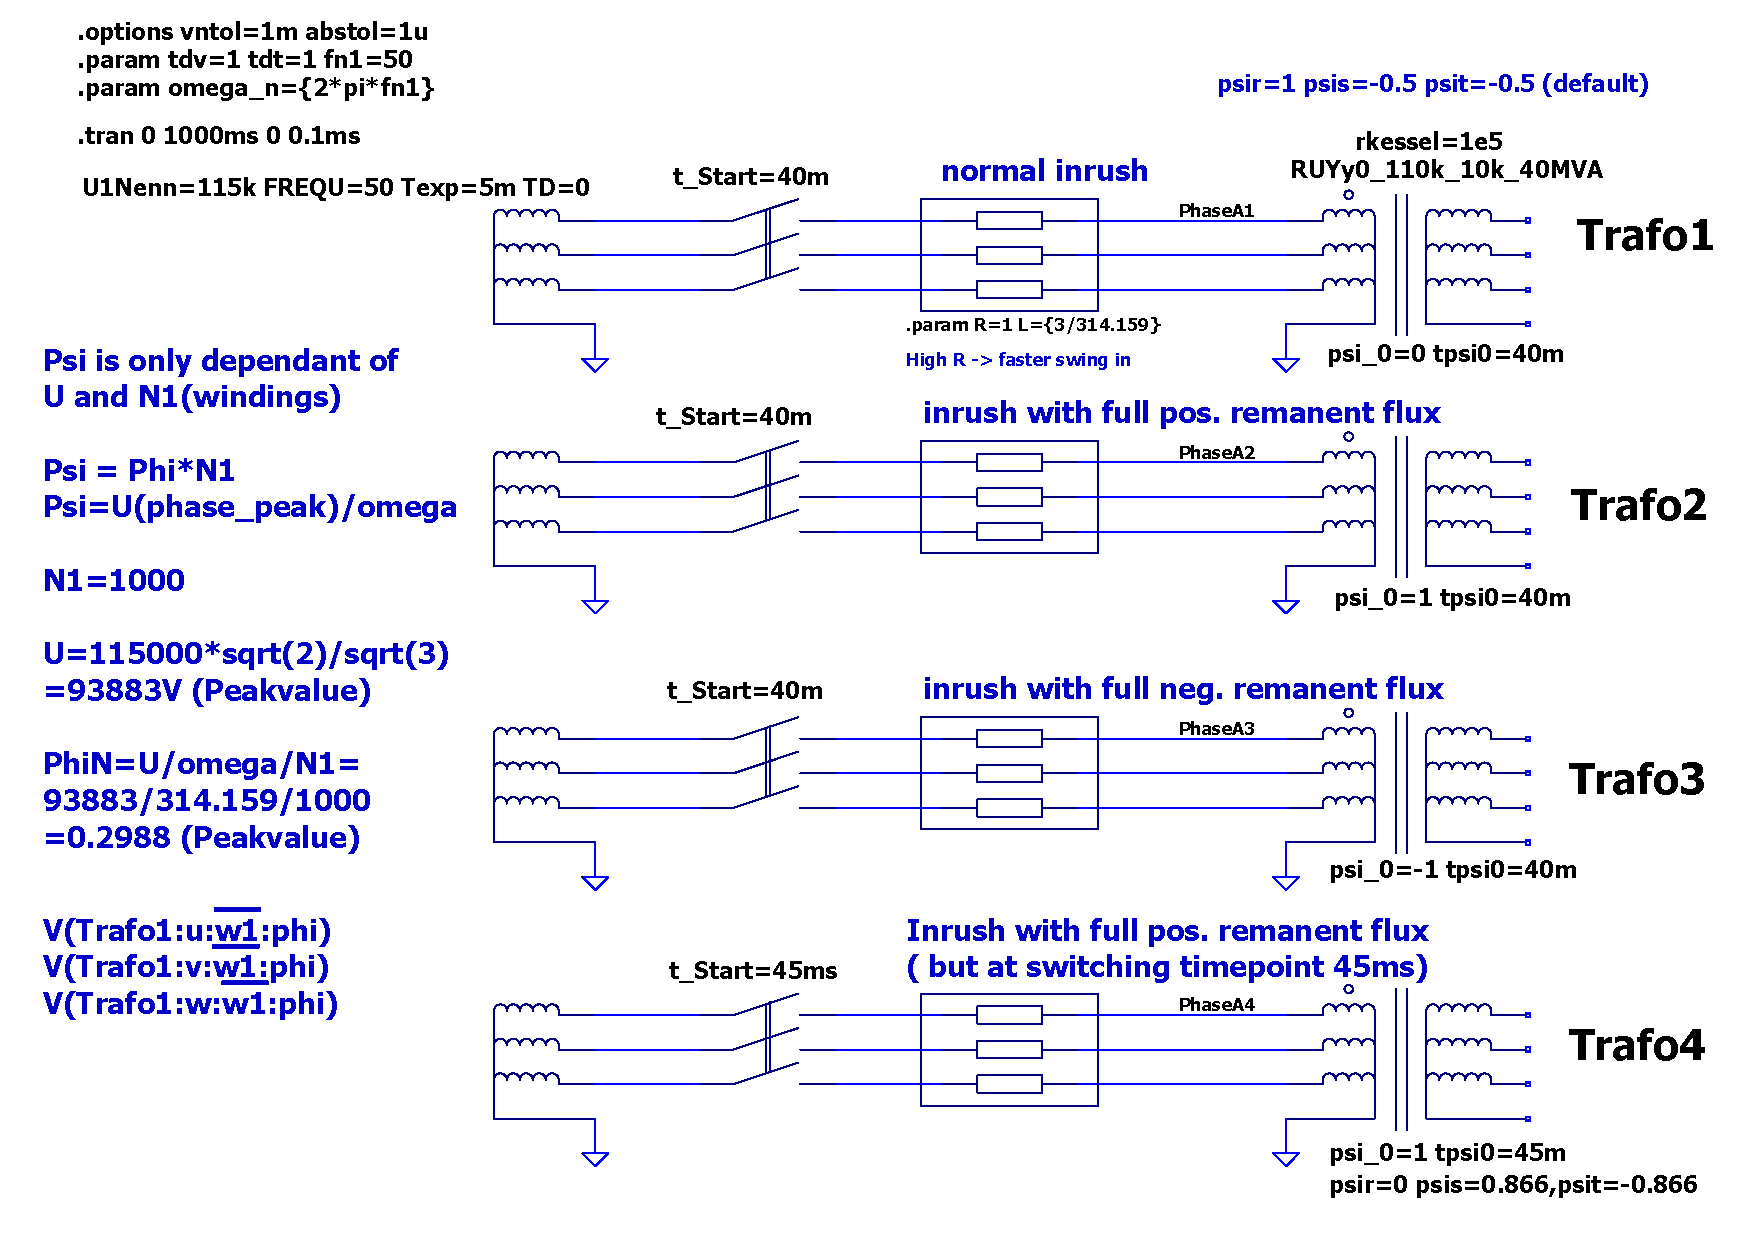
\includegraphics[width=1\textwidth] {figures/03_Initializing_Transformers_with_residual_flux/Initializing_Transformers_with_remanent_flux_Schematic}
	\caption{Initializing a Transformer with residual flux - schematic}
	\label{fig:figure31}
\end{figure}

\begin{figure}[H]
	\centering
	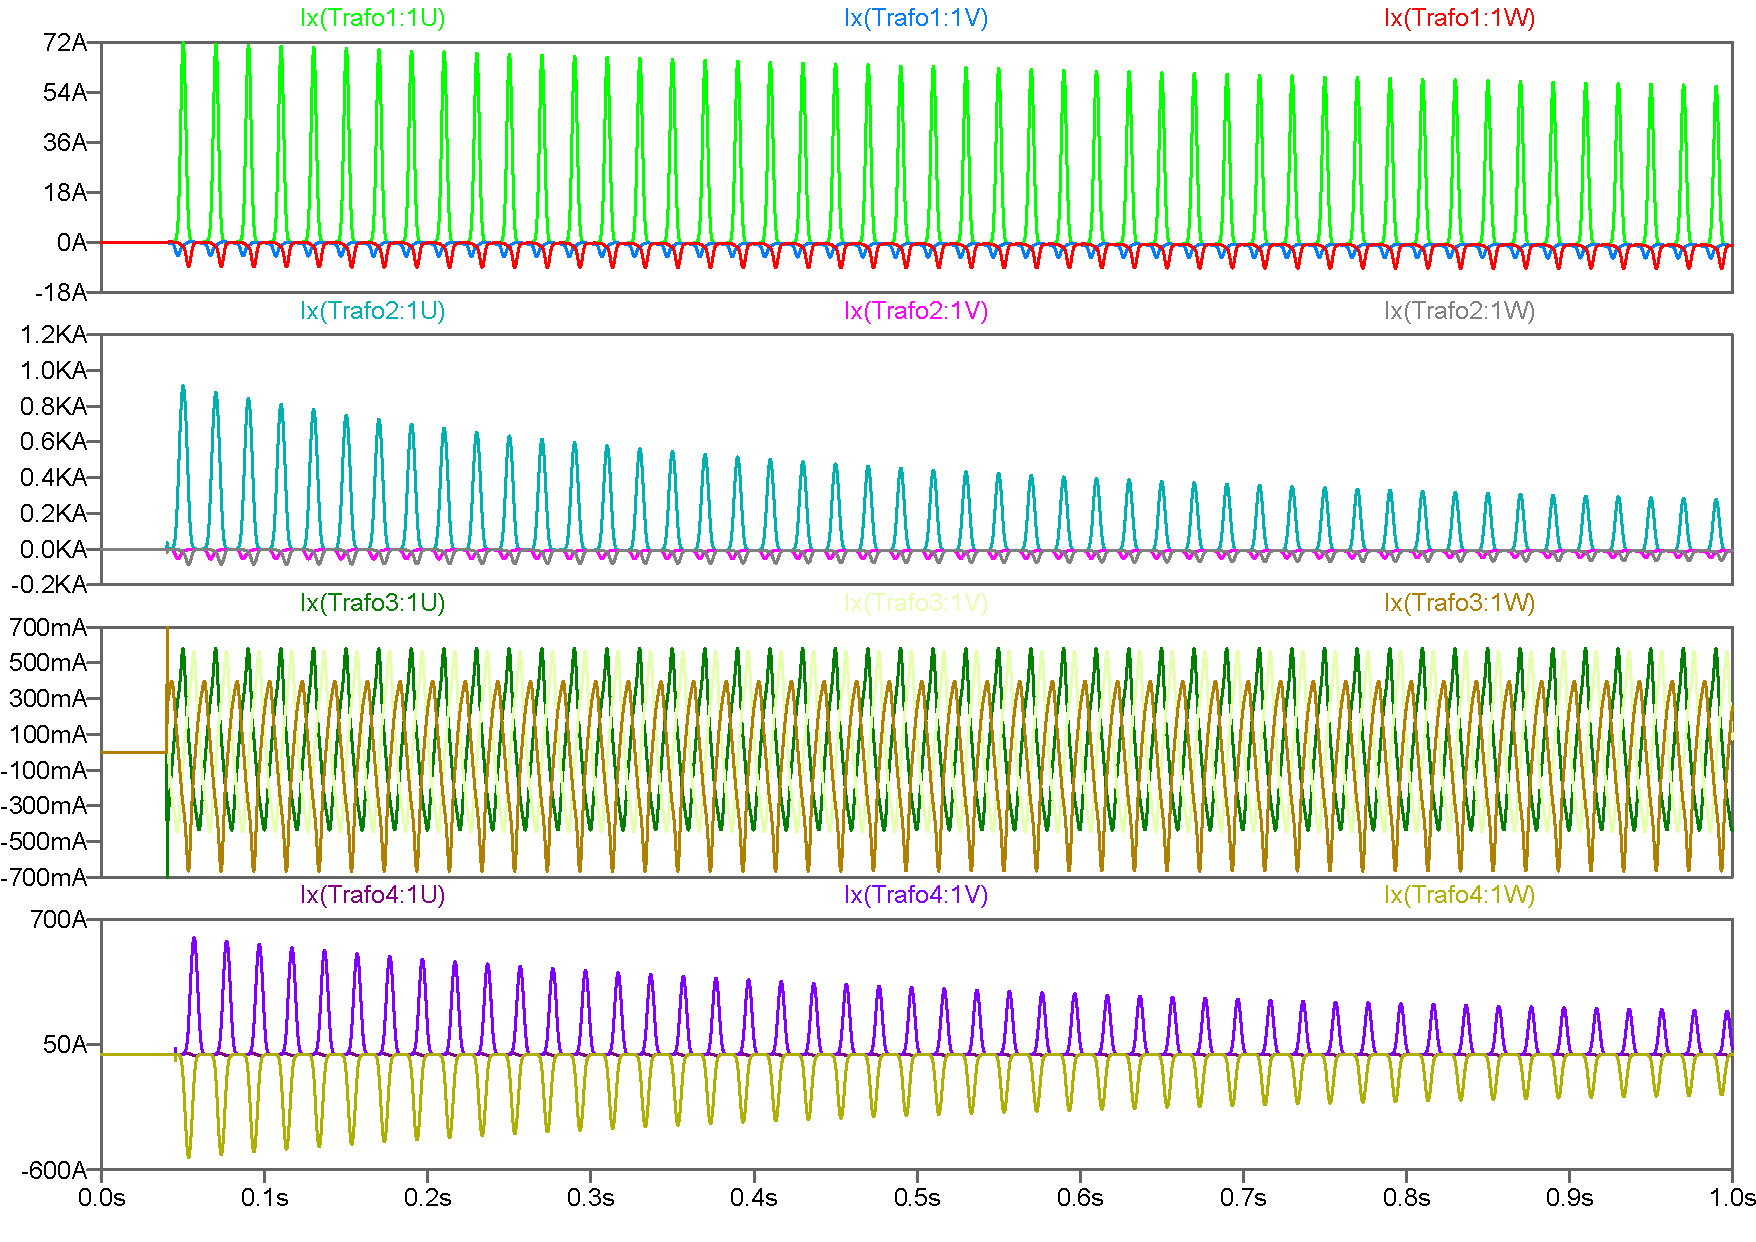
\includegraphics[width=0.9\textwidth] {figures/03_Initializing_Transformers_with_residual_flux/Initializing_Transformers_with_remanent_flux_waveform_of_currents}
	\caption{Initializing a Transformer with residual flux - Currents}
	\label{fig:figure32}
\end{figure}

\begin{figure}[H]
	\centering
	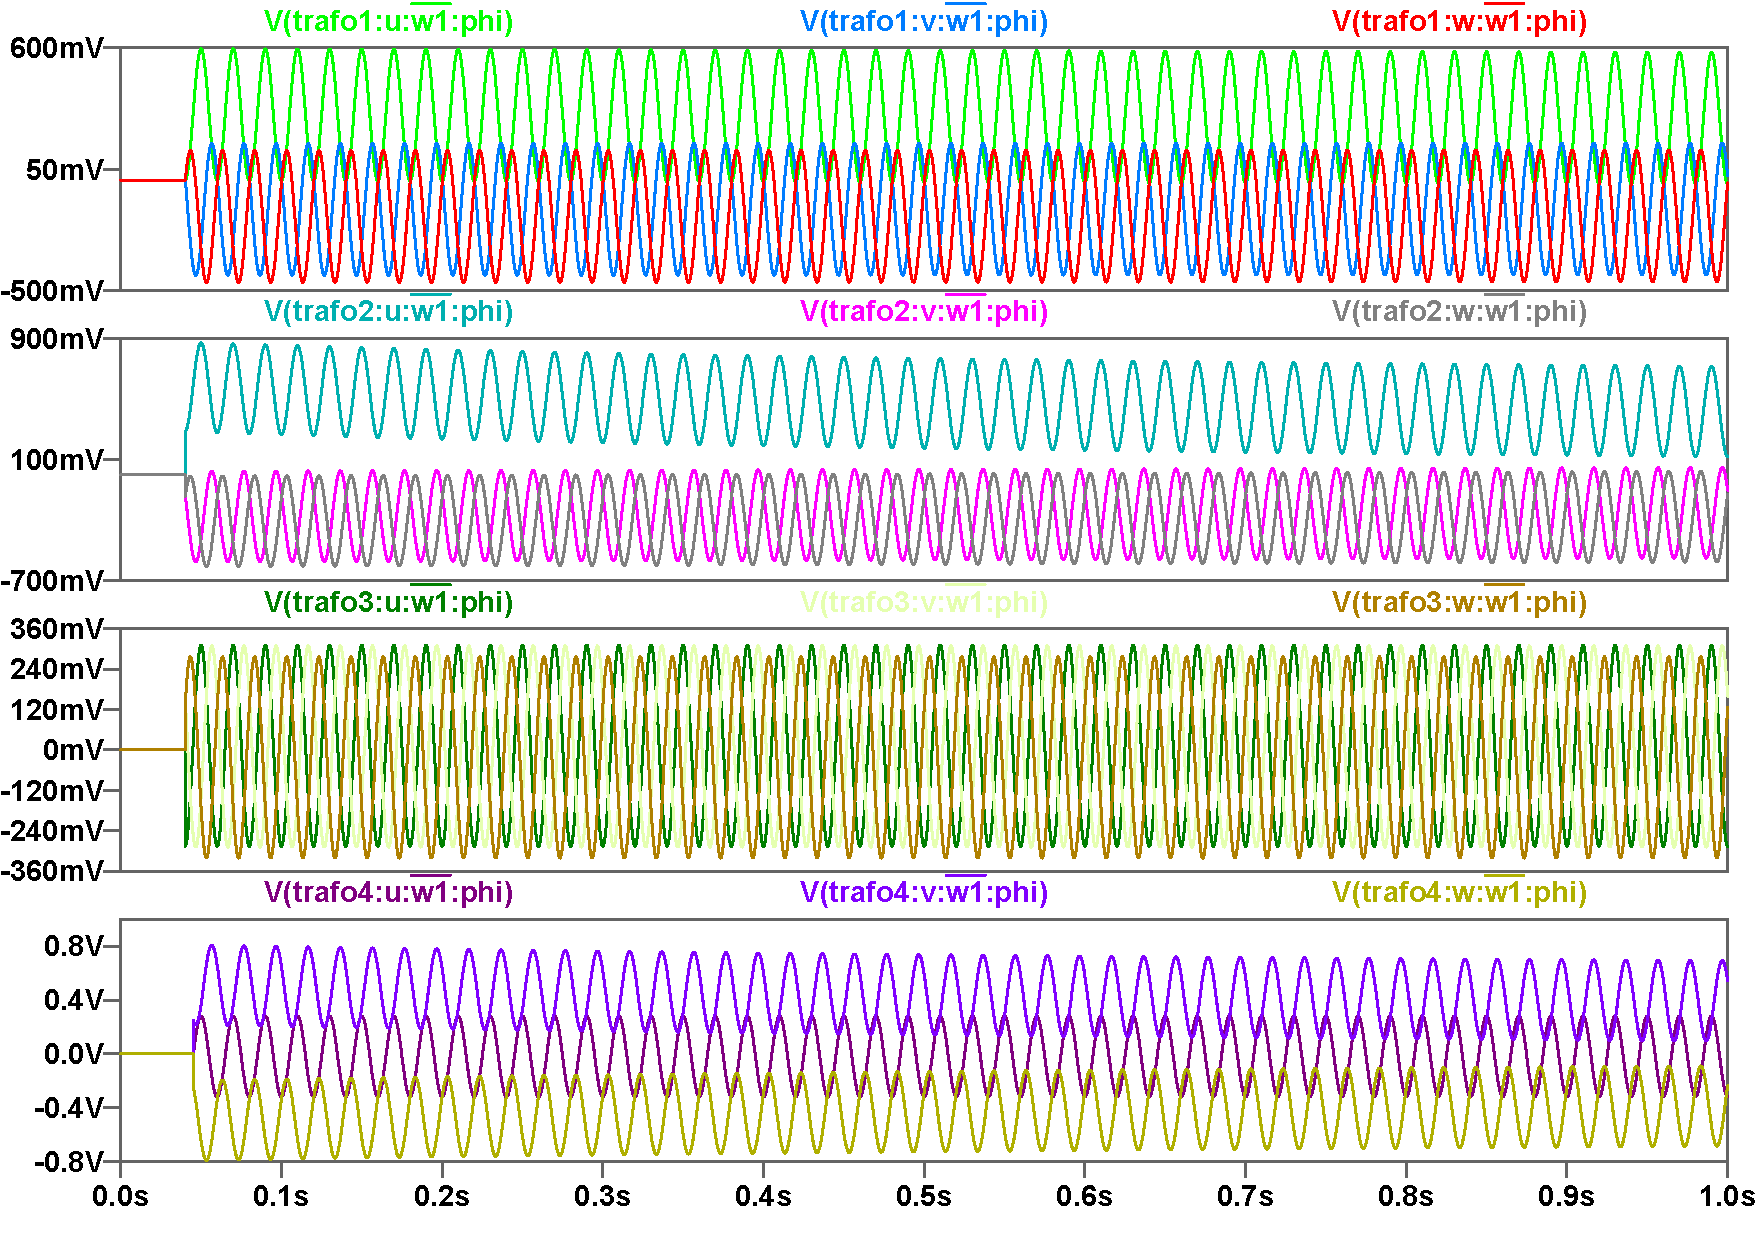
\includegraphics[width=0.9\textwidth] {figures/03_Initializing_Transformers_with_residual_flux/Initializing_Transformers_with_remanent_flux_waveform_of_fluxes}
	\caption{Initializing Transformer with residual flux - Fluxes}
	\label{fig:figure33}
\end{figure}


\begin{chaptersummary}
Transformer energization is governed by the integral of the applied voltage
and by the residual core flux at the switching instant. Closing at a voltage
zero crossing without residual flux can produce approximately twice the normal
steady-state peak flux. Unfavourable full residual flux can increase this to
about three times the normal peak and cause a large inrush current. Favourable
residual flux, controlled switching, or a gradual source-voltage ramp can
greatly reduce the transient. The initialization time and all three phase
residual-flux values must be coordinated with the switch closing instant.
Hint: It is often mentioned in the literature that the inrush current is attenuated by connecting the transformer to a load. However, this is not the case unless the load is truly very high—which, in turn, causes the total current to be very high, thereby masking the inrush current.
See LTspice example \texttt{Hidden\_inrush.asc} in this example folder
\end{chaptersummary}

\chapter{Switching Lines}
\label{chap:chapter4}
\index{line switching}
\index{cable!energization}
\index{Petersen coil}

\section{General}
\label{sec:section41}

This chapter examines the energization of unloaded and loaded cable lines. It
also considers the energization of a second line connected to an already
energized busbar and the energization of a cable terminated by a transformer.
The examples illustrate the influence of switching instant, line capacitance,
network inductance, load damping, and transformer residual flux on the
resulting transients.

The switching transients are oscillations at the natural frequencies of the
electrical network. Such oscillations occur whenever the system state changes
abruptly, for example during line energization or at the inception of an earth
fault or short circuit.

\section{Circuit Design}
\label{sec:section42}

Open the file: \texttt{switching\_lines.asc}. The LTspice schematic contains four circuits. Each line is a
\SI{5}{\kilo\metre}, \SI{110}{\kilo\volt} oil-filled cable with a conductor
cross-section of \SI{500}{\milli\metre\squared}. The circuits represent:

\begin{enumerate}
\item energization of an unloaded cable,
\item energization of a cable supplying a \SI{100}{\mega\watt} load,
\item energization of a second unloaded cable connected to an energized busbar,
\item energization of a cable terminated by a transformer with unfavourable
      full residual flux.
\end{enumerate}

Each single line is earth-fault compensated by a \SI{125}{\ampere} Petersen
coil. The double-line arrangement initially uses a compensation setting of \SI{125}{\ampere}, which is increased to\SI{250}{\ampere} at 400 ms. 


\subsection{Adjustment of the Petersen Coil}
\label{sec:petersen-adjustment}

To determine the required compensation, temporarily reduce the load in the
second circuit from \texttt{100e6} to \texttt{100e-6} and run the simulation.
The phase-1 charging-current peak is approximately \SI{60}{\ampere}. For a
shielded single-core cable whose dominant capacitances are phase-to-earth, the
earth-fault charging current is approximately

\begin{equation}
I_{\mathrm{E,peak}}\approx 3I_{0,\mathrm{peak}}
 =3\cdot\SI{60}{\ampere}=\SI{180}{\ampere},
\end{equation}

or approximately \SI{127}{\ampere} RMS. A \SI{125}{\ampere} Petersen coil is
therefore appropriate. After this adjustment, restore the load to
\texttt{100e6}.

\begin{remark}{Applicability of the threefold charging current}{remark41}
The relation $I_{\mathrm E}\approx3I_0$ applies to the zero-sequence charging
current of the cable. Overhead lines have appreciable phase-to-phase
capacitances, so the same simplified interpretation must not be transferred
without checking the complete capacitance matrix.
\end{remark}

\section{Energization of an Unloaded \SI{110}{\kilo\volt} Cable}
\label{sec:section43}
NOTE: Simulate \texttt{Switching\_lines.asc} and choose after simulation \texttt{line1.plt}.
This is done by activating the waveform-viewer window and click in the PlotSettings the menu item "open plot settings file".
 
For the selected switching instant, the Phase A switch closes near a voltage zero crossing. Its peak current is therefore the smallest, approximately
\SI{130}{\ampere}. Immediately after closing, the cable capacitances behave
like short circuits and draw large, rapidly changing charging currents. The
phase-2 and phase-3 current peaks reach approximately \SI{1.5}{\kilo\ampere}.
The oscillations have substantially decayed after approximately
\SI{200}{\milli\second}.

The Phase A voltage transient is likewise the smallest. The Phase B and
Phase C voltages reach approximately \SI{-160}{\kilo\volt} peak, about
\SI{30}{\percent} above the nominal phase-voltage peak. The precise current
and voltage maxima depend strongly on the switching instant. This can be
investigated by changing the switch parameter \texttt{t\_start} from
\SI{40}{\milli\second} to \SI{45}{\milli\second}.

\begin{important}{Origin of the voltage transient}{important41}
The capacitive charging current flows through the inductive source and line
impedances. The resulting voltage drop is superimposed on the source voltage
at the cable terminal. Consequently, the phases with the largest charging
current also show the largest voltage transient.
\end{important}

\subsection{Natural Frequency}
\label{sec:unloaded-line-natural-frequency}

The natural frequency can be identified in LTspice with
\textsc{View}/\textsc{FFT}. For example, an FFT of the Phase B voltage 
shows peaks at \SI{50}{\hertz} and approximately
\SI{1.44}{\kilo\hertz}.

The short-circuit power of the network is \SI{7.5}{\giga\volt\ampere}. Its
nominal reactance is

\begin{calculation}{Natural frequency of the \SI{5}{\kilo\metre} cable}{calculation41}
\begin{align}
X_{\mathrm N}
  &=\frac{U_{\mathrm N}^2}{S_{\mathrm k}}
    =\frac{(\SI{110}{\kilo\volt})^2}
           {\SI{7.5}{\giga\volt\ampere}}
    =\SI{1.613}{\ohm},\\
X_{\mathrm{line}}
  &=\SI{0.11}{\ohm\per\kilo\metre}\cdot\SI{5}{\kilo\metre}
    =\SI{0.55}{\ohm}.
\end{align}

With $\omega=2\pi\cdot\SI{50}{\hertz}$ and
$C'=\SI{400}{\nano\farad\per\kilo\metre}$, a lumped approximation gives

\begin{align}
L&=\frac{X_{\mathrm N}+X_{\mathrm{line}}}{\omega}
  \approx\SI{6.9}{\milli\henry},\\
C&=C'l=\SI{2}{\micro\farad},\\
f_{\mathrm r}&=\frac{1}{2\pi\sqrt{LC}}
  \approx\SI{1.35}{\kilo\hertz}.
\end{align}

The cable is implemented as a lumped T-section. During the initial charging
process, only the source-side half of its series inductance is effective in the
relevant resonant loop. Therefore,

\begin{align}
L_{\mathrm{eff}}
 &=\frac{X_{\mathrm N}+X_{\mathrm{line}}/2}{\omega}
   \approx\SI{6.0}{\milli\henry},\\
f_{\mathrm r,T}
 &=\frac{1}{2\pi\sqrt{L_{\mathrm{eff}}C}}
   \approx\boxed{\SI{1.45}{\kilo\hertz}},
\end{align}

which agrees closely with the simulated \SI{1.44}{\kilo\hertz}.
\end{calculation}

The approximate oscillation frequency can also be read directly in the waveform viewer:
zoom into two adjacent transient peaks and use the time difference and
frequency displayed in the lower-left status line.

\subsection{Petersen-Coil Oscillation}
\label{sec:petersen-oscillation}

The Petersen-coil voltage and current do not immediately reach steady state.
A slow beat of approximately \SI{1}{\hertz} is visible because the compensated
zero-sequence resonant frequency differs slightly from the network frequency.
After the transient has decayed, the residual coil current and beat are nearly
zero.

\section{Energization of a Loaded Line}
\label{sec:Section44}
NOTE: Simulate \texttt{Switching\_lines.asc} and choose after simulation \texttt{line2.plt}.
This is done by activating the waveform-viewer window and click in the PlotSettings the menu item "open plot settings file".
  
When the cable supplies the load, its voltage and current transients are more
strongly damped. The active part of the load absorbs oscillatory energy and
reduces the duration of the switching transient.

\section{Energization of a Second Line}
\label{sec:section45}
NOTE: Simulate \texttt{Switching\_lines.asc} and choose after simulation \texttt{line3.plt}.
This is done by activating the waveform-viewer window and click in the PlotSettings the menu item "open plot settings file".
  
The first, upper line is energized in the same way as the unloaded line in
\cref{sec:section43}. At \SI{400}{\milli\second}, the second line
is connected to the same busbar. The traces \texttt{Ix(Line3a:L1\_1)} and
\texttt{Ix(Line3b:L1\_1)} initially show transients of similar magnitude in both
lines.

Closer inspection shows that the high-frequency components have opposite
signs. They are capacitive currents circulating through the busbar and
the phase-to-earth capacitances of the two cables. For two identical
\SI{5}{\kilo\metre} cables, the approximate circulating-current frequency is

\begin{calculation}{Circulating-current and network-current frequencies}{calculation42}
\begin{align}
L_{\mathrm{ring}}
 &=\frac{2\cdot\SI{0.11}{\ohm\per\kilo\metre}
              \cdot\SI{2.5}{\kilo\metre}}
             {2\pi\cdot\SI{50}{\hertz}}
   \approx\SI{1.75}{\milli\henry},\\
C_{\mathrm{ring}}
 &=\frac{\SI{400}{\nano\farad}}{2}
   =\SI{200}{\nano\farad},\\
f_{\mathrm{ring}}
 &=\frac{1}{2\pi\sqrt{L_{\mathrm{ring}}C_{\mathrm{ring}}}}
   \approx\boxed{\SI{3.8}{\kilo\hertz}}.
\end{align}

The lower-frequency component drawn from the network source sees the combined
capacitance of both lines:

\begin{align}
L_{\mathrm{net}}
 &=\frac{\SI{1.613}{\ohm}
           +\SI{0.11}{\ohm\per\kilo\metre}\cdot\SI{2.5}{\kilo\metre}}
          {2\pi\cdot\SI{50}{\hertz}}
   \approx\SI{6.0}{\milli\henry},\\
C_{\mathrm{net}}&=2\cdot\SI{400}{\nano\farad}
   =\SI{800}{\nano\farad},\\
f_{\mathrm{net}}
 &=\frac{1}{2\pi\sqrt{L_{\mathrm{net}}C_{\mathrm{net}}}}
   \approx\boxed{\SI{1.03}{\kilo\hertz}}.
\end{align}
\end{calculation}

Because this network-current component has the lower frequency, its associated
inductive voltage drop and busbar-voltage transient are also smaller. The
reactive-power exchange of each cable can be viewed by holding \textsc{Alt}
and right-clicking the respective line element. LTspice then displays the
instantaneous product of element voltage and current.
The lower frequency can be observed by measuring the current at the voltage source. The higher frequency is measured by measuring the current flowing through the respective cable.

\section{Energization of a Transformer-Terminated Line}
\label{sec:section46}
NOTE: Simulate \texttt{Switching\_lines.asc} and choose after simulation \texttt{line4.plt}.
This is done by activating the waveform-viewer window and click in the PlotSettings the menu item "open plot settings file".
  
In the fourth circuit, the cable supplies a transformer initialized with
unfavourable residual flux. The transient current is therefore a combination
of capacitive cable-charging current and inductive transformer-inrush current.

In the Phase A closed at a voltage zero crossing, the capacitive contribution is
small while the inductive inrush contribution is large. In the other phases,
the capacitive component is initially dominant but decays rapidly; the
inductive component subsequently prevails. The two components decay at
different rates. Now extend the simulation to 15 s (\texttt{Switching\_lines\_15s.asc}) and run it again. During the first few seconds, the voltages on the primary side of the transformer exceed their nominal values. The Phase C voltage is particularly high. The peak value is 240kV compared to the nominal value of 90kV nominal peak voltage of line to ground voltage.
You can get this under control by operating the Petersen coil with slight undercompensation or overcompensation
(out of resonance). The residual-flux initialization and its coordination with the switching time are
described in \cref{chap:chapter3}.

\section{Extended-Line Study: Charging Current Near Rated Current}
\label{sec:section47}
\noindent NOTE: Simulate \texttt{Switching\_lines\_70km.asc} and choose after simulation for plotting \texttt{lines\_70km\_1.plt} for waveform1 or \texttt{lines\_70km\_2.plt} for waveform2

The cable length is increased until its steady-state charging current is close
to the nominal current of approximately \SI{900}{\ampere} peak, or
\SI{630}{\ampere} RMS. The simulation study uses a line length of
\SI{70}{\kilo\metre}.

For a phase-to-earth capacitance $C'$ and line-to-line RMS voltage
$U_{\mathrm{LL}}$, the approximate charging current is

\begin{equation}
I_{\mathrm c}=\omega C'l\frac{U_{\mathrm{LL}}}{\sqrt{3}}.
\label{eq:cable-charging-current}
\end{equation}

With $C'=\SI{400}{\nano\farad\per\kilo\metre}$, the ideal length required for
exactly \SI{600}{\ampere} RMS is about \SI{75}{\kilo\metre}. The
\SI{70}{\kilo\metre} simulation case is therefore a practical approximate
setting, with the exact result determined by the implemented line model.

At \SI{70}{\kilo\metre}, the current transient reaches approximately
\SI{3.5}{\kilo\ampere} in phase B and C, while its dominant oscillation frequency falls to
approximately \SI{230}{\hertz}. Despite the larger current, the voltage
transient is smaller and the oscillation decays rapidly. The greater cable
resistance provides stronger damping, and the lower oscillation frequency
reduces the network impedance.

\vspace{1cm}

\begin{calculation}{Comparison of inductive voltage drops across the network impedance}{calculation43}
For the \SI{5}{\kilo\metre} case,
\begin{align}
L_{\mathrm N}&=\frac{\SI{1.613}{\ohm}}
 {2\pi\cdot\SI{50}{\hertz}}\approx\SI{5.1}{\milli\henry},\\
X_L(\SI{1.44}{\kilo\hertz})
 &=2\pi\cdot\SI{1.44}{\kilo\hertz}\cdot L_{\mathrm N}
   \approx\SI{46.4}{\ohm},\\
\widehat U_L&\approx\SI{46.4}{\ohm}\cdot\SI{1.5}{\kilo\ampere}
  \approx\SI{69.6}{\kilo\volt}.
\end{align}

For the \SI{70}{\kilo\metre} case,
\begin{align}
X_L(\SI{230}{\hertz})
 &=2\pi\cdot\SI{230}{\hertz}\cdot L_{\mathrm N}
   \approx\SI{7.4}{\ohm},\\
\widehat U_L&\approx\SI{7.4}{\ohm}\cdot\SI{3.5}{\kilo\ampere}
  \approx\SI{25.9}{\kilo\volt}.
\end{align}
\end{calculation}

\vspace{1cm}

This explains why the \SI{70}{\kilo\metre} case produces a smaller voltage
transient even though its charging-current transient is larger. In LTspice,
the voltage drop can be measured by right-clicking the source-side terminal of the phase B impedance, choosing \textsc{Mark Reference}, and selecting the switch-side terminal of the impedance
 as the second measurement point. The observed drop is approximately
\SI{25}{\kilo\volt}, compared with approximately \SI{70}{\kilo\volt} in the
\SI{5}{\kilo\metre} case. This is because the dominant frequency is much lower and therefore the impedance is much smaller. HINT: Observe the Petersen-coil current in the \SI{70}{\kilo\metre} cable network. Its peak value is approximately \SI{90}{\ampere}.  

\newpage

\begin{figure}[H]
	\centering
	\includegraphics[width=1\textwidth] {figures/04_Switching\_lines/Switching\_lines\_schematic}
	\caption{Switching lines - schematic}
	\label{fig:figure41}
\end{figure}

\begin{figure}[H]
	\centering
	\includegraphics[width=0.9\textwidth] {figures/04_Switching\_lines/Switching\_lines\_waveforms1}
	\caption{Switching lines1 - waveform}
	\label{fig:figure42}
\end{figure}

\begin{figure}[H]
	\centering
	\includegraphics[width=0.9\textwidth] {figures/04_Switching\_lines/Switching\_lines\_waveforms2}
	\caption{Switching lines2 - waveform}
	\label{fig:figure43}
\end{figure}

\begin{figure}[H]
	\centering
	\includegraphics[width=0.9\textwidth] {figures/04_Switching\_lines/Switching\_lines\_waveforms3ab}
	\caption{Switching lines3 - waveform}
	\label{fig:figure44}
\end{figure}

\begin{figure}[H]
	\centering
	\includegraphics[width=0.9\textwidth] {figures/04_Switching\_lines/Switching\_lines\_waveforms4}
	\caption{Switching lines4 - waveform}
	\label{fig:figure45}
\end{figure}

\begin{figure}[H]
	\centering
	\includegraphics[width=0.9\textwidth] {figures/04_Switching\_lines/Switching\_lines\_15s_waveform}
	\caption{Switching lines 15s - waveform}
	\label{fig:figure48}
\end{figure}

\begin{figure}[H]
	\centering
	\includegraphics[width=1\textwidth] {figures/04_Switching\_lines/Switching\_lines\_70km_schematic}
	\caption{Switching lines 70km - schematic}
	\label{fig:figure46}
\end{figure}

\begin{figure}[H]
	\centering
	\includegraphics[width=0.9\textwidth] {figures/04_Switching\_lines/Switching\_lines\_70km_waveform1}
	\caption{Switching lines 70km - waveform1}
	\label{fig:figure47}
\end{figure}

\begin{figure}[H]
	\centering
	\includegraphics[width=0.9\textwidth] {figures/04_Switching\_lines/Switching\_lines\_70km_waveform2}
	\caption{Switching lines 70km - waveform2}
	\label{fig:figure48}
\end{figure}



\begin{chaptersummary}
Cable energization produces high-frequency oscillations determined mainly by
network inductance and cable capacitance. The switching instant controls the
initial phase currents and overvoltages, while a connected load increases
damping. Energizing a second cable creates both high-frequency circulating
currents and a lower-frequency network-current component. When a cable
supplies a transformer, capacitive charging and inductive inrush currents are
superimposed. Increasing the cable length raises the charging current but also
lowers the resonant frequency and increases resistive damping; the resulting
voltage transient can therefore become smaller even when the current transient
is larger. As can be seen in the example with the transformer, operating the Petersen coil exactly at the resonance point can cause very high voltages. For this reason, in practice, the Petersen coil is operated with either slight overcompensation or undercompensation. As can be seen in the network with the \SI{70}{\kilo\meter} cable, the residual current in very large cable networks becomes quite high. The network is therefore usually divided into smaller subnetworks.
\end{chaptersummary}

\chapter{Earth Faults in \SI{110}{\kilo\volt} and \SI{10}{\kilo\volt} Power Grids}
\label{chap:earth-faults}
\index{earth fault}
\index{Petersen coil}
\index{resonant grounding}
\index{neutral displacement voltage}

\section{General}
\label{sec:earth-fault-general}

A Petersen coil is an intelligent protection and stabilization element in medium-voltage networks and, in some cases, also in high-voltage networks. It ensures that single-phase earth faults can be controlled safely and without immediate shutdown. This makes it an indispensable component of modern power supply systems.
The Petersen coil is an inductive coil that is connected to the neutral point of the transformer. In a three-phase AC network, capacitive currents flow between conductors and earth. If a ground fault occurs, a capacitive fault current flows through the fault location – this can be dangerously high.
In the event of a fault, the Petersen coil generates an inductive current that is opposes the capacitive fault current and, in the ideal case, compensates for it at the fault location.

\section{Circuit design}

This chapter investigates earth faults in small cable networks with resonant neutral grounding. The first example is the simulation file \texttt{Petersen\_without\_Fault\_TRAN.asc}. The principal \SI{110}{\kilo\volt} example is designed for
a nominal earth-fault compensation current of \SI{300}{\ampere}. In normal
operation, network asymmetry produces only a small neutral displacement
voltage and therefore a small Petersen-coil current. During a solid earth
fault, approximately the full phase-to-earth voltage appears between the
transformer neutral and earth, and the coil supplies approximately its rated
current.

Unless stated otherwise, the transformer is unloaded. The earth fault is
applied at \SI{205}{\milli\second}. The voltage-source parameter
\texttt{texp} is used to establish steady state rapidly before the fault. The
model contains a Yd5 transformer whose parameters are defined in the LTspice file \texttt{Transformer\_110k\_10k.asc}

\section{Compensated \SI{110}{\kilo\volt} Network Without a Fault}
\label{sec:Compensated Network Without a Fault}

\subsection{Adjustment of the Petersen Coil}
\label{sec:Adjustment of the Petersen Coil}

The network has a phase-to-earth capacitance of \SI{5012}{\nano\farad} per phase. At \SI{50}{\hertz}, its capacitive reactance is ..

\begin{calculation}{Petersen-coil rating from the network capacitance}{calculation51}
\begin{align}
X_C&=\frac{1}{\omega C}
 =\frac{1}{2\pi\cdot\SI{50}{\hertz}\cdot\SI{5012}{\nano\farad}}
 \approx\SI{635.1}{\ohm},\\
I_C&=\frac{U_{\mathrm{LL}}/\sqrt{3}}{X_C}
 =\frac{\SI{110}{\kilo\volt}/\sqrt{3}}{\SI{635.1}{\ohm}}
 \approx\SI{100}{\ampere}\ \text{RMS}.
\end{align}

For a single-phase earth fault, the total capacitive earth-fault current is
approximately three times the phase charging current. Resonant compensation
therefore requires

\begin{align}
I_{\mathrm P}&\approx3I_C=\SI{300}{\ampere},\\
X_{L,\mathrm P}&=\frac{X_C}{3}
 \approx\boxed{\SI{211.7}{\ohm}}.
\end{align}
\end{calculation}

The Petersen-coil model accepts the nominal line-to-line voltage and
compensation current directly. We set these to \SI{110}{\kilo\volt} and
\SI{300}{\ampere}.

\subsection{Neutral Displacement Voltage in the Transient Analysis}
\label{sec:Neutral Displacement Voltage in the Transient Analysis}

Even without a fault, unequal phase-to-earth capacitances produce a neutral
displacement voltage across the Petersen coil. In this example, its peak value is
approximately \SI{1.2}{\kilo\volt} peak, much smaller than the rated phase voltage.
The greater the difference between the phase capacitances, represented in the
model by \texttt{CE+CE1} and \texttt{CE}, the higher this voltage becomes.

The displacement voltage rises slowly and shows a beat frequency of
approximately \SI{1.2}{\hertz}. This indicates that the resonant frequency is
not exactly \SI{50}{\hertz}. In the LTspice waveform viewer, the beat frequency
can be read by drawing a zoom window between two adjacent maxima and observing
the frequency in the status line. (See figure \ref{fig:Figure1})
 

\subsection{Corrected Petersen-Coil Setting}
\label{sec:Corrected Petersen-Coil Setting}

The capacitance-only calculation in calculation \ref{calc:calculation51} is correct for
an ideal transformer, but the complete resonant circuit is not optimally compensated
with a \SI{300}{\ampere} coil. The transformer short-circuit reactance on the primary side,
$X_{\mathrm{1s}}=\SI{30.25}{\ohm}$ (see \texttt{Transformer\_110k\_10k.asc}) , reduces the
resonant frequency to \SI{48.8}{\hertz}. The coil nominal current must
therefore be increased to approximately \SI{315}{\ampere} to get again \SI{50}{\hertz}. This can be verified by simulating with \texttt{Petersen\_without\_Fault\_AC.asc}. (See figure \ref{fig:Figure2})

Now we set the initially choosen value of
1E20 for the magnetic reluctance of the transformer tank to a reasonable value of 1e6. After running the simulation, we find that the resonant frequency is again below \SI{50}{\hertz}. 

We now choose \SI{328}{\ampere} for the Petersen coil. We restart the simulation. Now we see that the resonant point is again at approximately \SI{50}{\hertz}. We have seen now that the compensation current calculated from the total cable capacitance alone differs from the required Petersen-coil setting because of the transformer’s internal impedance. We have to add about 10\% for the Petersen current value to compensate for the voltage drop at the starpoint.

\begin{remark}{Phase information in AC analysis}{rem:automatic-Petersen}
	In practice, the automatic Petersen-coil controller normally maintains slight overcompensation or undercompensation to avoid resonance. Additionally the controller is disabled when an earth fault occurs to prevent further drift.
\end{remark}

\subsection{Reason about the reduction of the starpoint voltage}
 
Explanation of the Reduced Neutral-Point Voltage when adding the magnetic reluctance of the transformer tank lies in the additional secondary leakage flux and the corresponding voltage drop across the leakage reactance. This further decreases the effective neutral‑point voltage.
You can clearly see this in the file \texttt{Petersen\_with\_fault\_hierarchical\_model\_AC.asc}. After simulation click on the transformer symbol then open schematic. Then click on the symbol for the primary winding Phase A and open schematic again. Then measure the current through RPhis. This gives approximately 9 mA (This current models the flux value in Wb). Perform the same measurement for the secondary winding above the primary winding. The current there is 7 mA increasing now the sum of all leakage fluxes. The Resonant frequency is approximately 47.9Hz. (See figure \ref{fig:Figure4})


\subsection{Resonance Frequency at about 50Hz}
\label{sec:Resonant Frequency at about 50Hz}
This is the resonance of all three phase capacitances with the Petersen-coil
inductance and the effective transformer leakage inductance in the
zero-sequence path. The coil reactance and inductance are

\begin{align}
	X_{\mathrm P}&=\frac{U_{\mathrm{LL}}}{\sqrt{3}I_{\mathrm P}}
	=\frac{\SI{110}{\kilo\volt}}{\sqrt{3}\cdot\SI{300}{\ampere}}
	\approx\SI{211.7}{\ohm},\\
	L_{\mathrm P}&=\frac{X_{\mathrm P}}{2\pi\cdot\SI{50}{\hertz}}
	\approx\SI{0.674}{\henry}.
\end{align}

The transformer leakage reactance gives

\begin{equation}
	L1s=\frac{\SI{30.25}{\ohm}}
	{2\pi\cdot\SI{50}{\hertz}}\approx\SI{0.096}{\henry}.
\end{equation}

Since the three phase capacitances act in parallel and the three transformer
phase inductances contribute as $L1s_{}/3$ 


\begin{calculation}{Resonanz at 50Hz without leakage inductance}{Calculation52}
	\begin{align}
		C_0&=3\cdot\SI{5012}{\nano\farad},\\
		L_0&=L_{\mathrm P}+\frac{L1s}{3}
		=\SI{0.674}{\henry},\\
		f_{\mathrm r,0}&=\frac{1}{2\pi\sqrt{L_0C_0}}
		\approx\boxed{\SI{50}{\hertz}}.
	\end{align}
\end{calculation}

\begin{calculation}{Resonanz at 48.8Hz with primary leakage inductance}{Calculation53}
	\begin{align}
		C_0&=3\cdot\SI{5012}{\nano\farad},\\
		L_0&=L_{\mathrm P}+\frac{L1s}{3}
		=\SI{0.674}{\henry}+\frac{\SI{0.096}{\henry}}{3},\\
		f_{\mathrm r,0}&=\frac{1}{2\pi\sqrt{L_0C_0}}
		\approx\boxed{\SI{48.8}{\hertz}}.
	\end{align}
\end{calculation}

\begin{calculation}{Resonanz at 47.9Hz also with secondary leakage inductance}{Calculation54}
	\begin{align}
		C_0&=3\cdot\SI{5012}{\nano\farad},\\
		L_0&=L_{\mathrm P}+\frac{L1s}{3}+\frac{L1s*7}{9}
		=\SI{0.674}{\henry}+\frac{\SI{0.096}{\henry}}{3}+\frac{\SI{0.096}{\henry}*7}{9},\\
		f_{\mathrm r,0}&=\frac{1}{2\pi\sqrt{L_0C_0}}
		\approx\boxed{\SI{47.95}{\hertz}}.
	\end{align}
\end{calculation}

7/9 means the relation of the leakage fluxes measured above (9 Wb and 7 Wb).  
The resonant peaks for 48.8 Hz and 47.95 Hz can also be observed in the file\\
\texttt{Petersen\_without\_fault\_AC.asc}. 
by setting rkessel (this is the parameter for tank reluctance) to 1e6 or 1e20.
For the calculation of the resonant frequencies see also the file \texttt{Petersen.asc}



\section{Low-Resistance Earth Fault in the \SI{110}{\kilo\volt} Network}
\label{sec:110kv-low-resistance-earth-fault}

\subsection{Network Compensated with \SI{328}{\ampere} }
\label{sec:300a-earth-fault}

The transient simulation is contained in
\texttt{Petersen\_with\_fault\_TRAN.asc} (see figure \ref{fig:Figure5a}). At fault inception, the phase-R voltage
rapidly collapses to zero. The voltages of the two healthy phases rise toward
the line-to-line voltage. This transition is accompanied by high-frequency
overvoltages and currents. An FFT shows a mixture of dominant components near
\SI{260}{\hertz} and \SI{1.2}{\kilo\hertz}. (see figure \ref{fig:Figure13}) .

At this higher frequency, the capacitive reactance decreases and the
inductive reactance of the line impedance increases. The capacitive current
through the inductive impedance therefore produces an additional voltage rise.
The currents flowing toward the transformer are predominantly inductive and
approximately in phase with one another. Their inductive character can be
recognized because the current maximum lags the corresponding voltage maximum.
You can also see that the voltages of the healthy phases have a phase difference going from
120 degrees to 60 degrees (see figure \ref{fig:FigureX})

The current at the fault location initially reaches approximately
\SI{4.2}{\kilo\ampere} peak (see figure \ref{fig:Figure5}). It decays rapidly and approaches approximately a steady-state peak value of approximately \SI{4}{\ampere} peak. Its minimum also depends on the ohmic resistance of the Petersen coil, set by \texttt{r\_x} parameter.
The prefault capacitive reactive power is approximately \SI{-6.3}{\mega\varunit} per phase, or about
\SI{-19}{\mega\varunit} in total. Immediately after the phase A fault, the
high-frequency recharging process briefly drives the phase B and phase C
values to approximately \SI{-40}{\mega\varunit}. However, immediately after the fault. The capacitive and inductive reactive-power components are superimposed. The reason for the doubling of the capacitive reactive power is that the two
capacitances of the healthy phases are suddenly subjected to a voltage √3 times the normal phase-to-earth voltage. At the end of the transient processes, the additional capacitive reactive power is again compensated by the Petersen reactor. In addition, the inductive reactive power decays to zero. In the end, the reactive power is exactly the same as it was at the beginning (see figure \ref{fig:Figure5} and \ref{fig:Figure6}). In \texttt{Petersen\_with\_Fault\_AC.asc}, the minimum fault
current is approximately \SI{3}{\ampere} RMS near \SI{50}{\hertz} (see figure \ref{fig:Figure6}). Set the vertical axis to linear scaling to read this minimum accurately.
You can also see that the voltage magnitude of phase A is zero, and that Phase B and Phase C are at 111 kV, which is the phase‑to‑phase voltage.The phase angle of phase B is −150°, and that of phase C is +150°. The difference is −150 − 150 = −300 = +60 degrees, just as we observed earlier. (see figure \ref{fig:FigureX})


 


\begin{remark}{Phase information in AC analysis}{rem:earth-fault-ac-phase}
The relative phase angles of voltages and currents are most accurately
examined in the AC-analysis files, where the fundamental-frequency phasors are
not obscured by the switching transient.
\end{remark}

\subsection{Reactive Power detailed}
\label{sec:earth-fault-reactive-power}

The capacitive reactive power of the network is approximately

\begin{equation}
	Q_C=\sqrt{3}\,U_{\mathrm{LL}}I_C
	=\sqrt{3}\cdot\SI{110}{\kilo\volt}\cdot\SI{100}{\ampere}
	\approx\SI{19}{\mega\varunit}.
	\label{eq:network-capacitive-reactive-power}
\end{equation}

It can be measured with the \texttt{qmeter\_uvw} element. Each phase contributes
approximately \SI{-6.3}{\mega\varunit}, with small differences caused by the
unequal capacitances and the resulting unequal phase voltages (This explains the neutral displacement voltage). The waveform
viewer shows approximately \SI{110}{\kilo\volt},
\SI{111.7}{\kilo\volt}, and \SI{110.7}{\kilo\volt} after the model's display
scaling by $\sqrt{3}/\sqrt{2}$. Their mean is slightly above
\SI{110}{\kilo\volt} because the capacitive current produces a voltage rise
across the inductive line impedance.

\begin{remark}{Waveform-viewer units and scaling}{rem:qmeter-scaling}
	Multiplying a power trace by \texttt{1W/1V} can be used to change the displayed
	unit prefix in the waveform viewer. If \texttt{sfactor=3} is selected in
	\texttt{qmeter\_uvw}, the measured values are multiplied internally by three,
	which may simplify comparison with the total three-phase power.
\end{remark}


\subsection{Reactive-Power Increase at Fault Inception}
\label{sec:earth-fault-reactive-power-doubling}

During the earth fault, the two healthy phase-to-earth capacitances are charged
to approximately the line-to-line voltage, while the capacitance of the
faulted phase is discharged. Since capacitive reactive power is proportional
to voltage squared, the total capacitive reactive power of the healthy phases
is ideally twice (because of the voltage transients even higher) the prefault three-phase value. The source current therefore
also rises correspondingly.

After the transient, one part of this increased capacitive earth-fault current
is compensated by the Petersen coil. The ordinary positive-sequence charging
current remains supplied by the source.


\subsection{Additional Transformer Loading Due to Petersen-Coil Current}
\label{sec:petersen-transformer-loading}

The Petersen-coil current flows through the transformer windings and therefore
adds to the transformer loading. In the example, its equivalent contribution
is approximately \SI{100}{\ampere} per phase, while the rated primary current
is approximately \SI{200}{\ampere}. Because this current is predominantly
inductive, it must be added vectorially to the load current. For the assumed
load, whose reactive component is about one fifth of its active component,
approximately \SI{90}{\percent} of the original load capability remains.
NOTE: The additional load due to the Petersen is only present when a earth-fault
occur. In addition, we must take into account the high secondary-side circulating current resulting from the inclusion of the transformer tank in the simulation which also puts a  certain load on the transformer.
This is seen best in the file \texttt{Petersen\_without\_fault\_hierarchical\_model\_TRAN/AC.asc}.
Right-click the transformer symbol and select \texttt{Open Schematic}. After running the simulation, measure the current in the secondary winding of Phase A. 

\subsection{Loaded and Unloaded Transformer}
\label{sec:loaded-unloaded-transformer-earth-fault}

Changing the load parameter from \texttt{20e-6} to \texttt{40e6} reduces both
the phase voltages and the transformer neutral voltage. Since the voltage
across the cable capacitances decreases at the same time, the compensation
tuning remains almost unchanged. The comparison is implemented in
\texttt{Petersen\_with\_fault\_with\_load\_vs\_without\_load\_AC.asc}.
(see figure \ref{fig:Figure7a} and \ref{fig:Figure7})
NOTE: The Petersen current in the unloaded case is higher (304A) because of higher voltage level of 111.4kV compared to the loaded case where the voltage level is 110kV and the current is (300A). 

\section{High-Resistance Earth Fault}
\label{sec:110kv-high-resistance-earth-fault}

The AC-analysis file \texttt{Petersen\_with\_fault\_highohmic\_AC.asc}
compares the earth-fault resistances \SI{50}{\ohm}, \SI{100}{\ohm},
\SI{500}{\ohm}, and \SI{1000}{\ohm}. At the resonance point, all current
curves approach approximately \SI{3}{\ampere}, representing the residual
ohmic component of the compensated earth-fault current.
(see figure \ref{fig:Figure8a} and \ref{fig:Figure8})

\section{Comparison of coupled and uncoupeled line impedance}
\label{sec:coupled-uncoupled}
Open \texttt{Petersen\_fault\_coupled\_uncoupled.asc} and run the simulation.
After simulation we see that the peak fault current is lower in the coupled-line case than in the uncoupled-line case. The difference is about \SI{1}{\kilo\ampere}. The steady state current at the end of the simulation is the same for the two cases. 
This shows that simulating a asymmetric fault the coupling of the lines has to be
considered. For the calculation of the coupled impedance values see also the wxmaxima file \texttt{Petersen.asc}\\
(see figure \ref{fig:Figure9a} and \ref{fig:Figure9})

\begin{important}{Asymmetric faults}{}
	Coupling must be included when simulating asymmetrical faults in coupled-line systems.
\end{important}


\section{Compensated \SI{10}{\kilo\volt} Network with a Grounding Transformer}
\label{sec:grounding-transformer}
A Yd transformer does not provide an accessible neutral on its delta-connected
side. An external neutral-forming transformer, represented by
\texttt{Trafo\_gnd} symbol, creates a neutral point in the medium-voltage network without presence of a transformer with starpoint so that a Petersen coil can be connected. The corresponding simulation files are

\begin{itemize}
	\item \texttt{Petersen\_Trafo\_gnd\_TRAN.asc},
	\item \texttt{Petersen\_Trafo\_gnd\_AC\_fault.asc},
	\item \texttt{Petersen\_Trafo\_gnd\_AC\_no\_fault.asc}.
\end{itemize}

We now see a \texttt{\SI{10}{\kilo\volt}} compensated network with external grounding transformer. You see a Petersen in a medium voltage network. Due to the star point builder, a YD transformer can establish a star point at the secondary side for connecting a Petersen coil. 

\section{Petersen-coil and Yy-Transformers with three legs} 

Now consider a Petersen coil connected to a Yy transformer with a three-leg core. Since the YY transformer has no low-reluctance return path for zero-sequence flux in the core of the transformer, the flux must return through the tank and oil. This is not the goal. Therefore, the star point of a wye/wye transformer should only be loaded to no more than 10\% of the transformer’s rated current. See \texttt{ThreeLegCore-Yy-Transformer.asc}

\section{Solid Neutral Earthing and a Yy-Transformer with a Five-Leg Core}
Open the File \texttt{FiveLegCore\_without\_third\_winding.asc}. If the Yy-transformer has a five leg core, the star point cannot deliver any current if the second star point is isolated. This is because the outer legs provide a low-reluctance return path for in-phase fluxes. If the second star point is also connected, current can flow from one into the other star points, but current should not be exchanged between the two star points. In short, the two star points of a five leg Yy-transformer should be isolated. Now open file \texttt{FiveLegCore\_with\_third\_winding.asc}. Now consider neutral-point loading in a Yy transformer with a five-leg core and a compensating tertiary winding. The transformer can deliver full current at the star points. There is also no current transfer from one to the other star point.

\section{Characteristic Resonance Frequencies}
\label{sec:earth-fault-resonance-frequencies}

Several natural frequencies occur after fault inception. The highest is
associated with the discharging capacitance of the faulted phase. A lower
frequency appears in the healthy-phase voltages and capacitance currents.



\subsection{Resonance at \SI{1.2}{\kilo\hertz}}

This resonant path contains the cable series inductance and the faulted phase
capacitance. It is driven mainly through capacitor C12 and the fault position.
With $L=\SI{3.5}{\milli\henry}$ and
$C=\SI{5022}{\nano\farad}$ follows ..

\begin{equation}
	f_{\mathrm r}=\frac{1}{2\pi\sqrt{LC}}
	\approx\boxed{\SI{1.2}{\kilo\hertz}}.
\end{equation}


\subsection{Resonance at \SI{260}{\hertz}}

This is the frequency of the current through the netimpedance
and the capacities C10 and C11.
With $L=\SI{25}{\milli\henry}$ and $C=\SI{5012}{\nano\farad}$*3


\begin{equation}
	f_{\mathrm r}=\frac{1}{2\pi\sqrt{LC}}
	\approx\boxed{\SI{260}{\hertz}}.\\
\end{equation}

For the frequencies see figure \ref{fig:Figure13}

\begin{figure}[H]
	\centering
	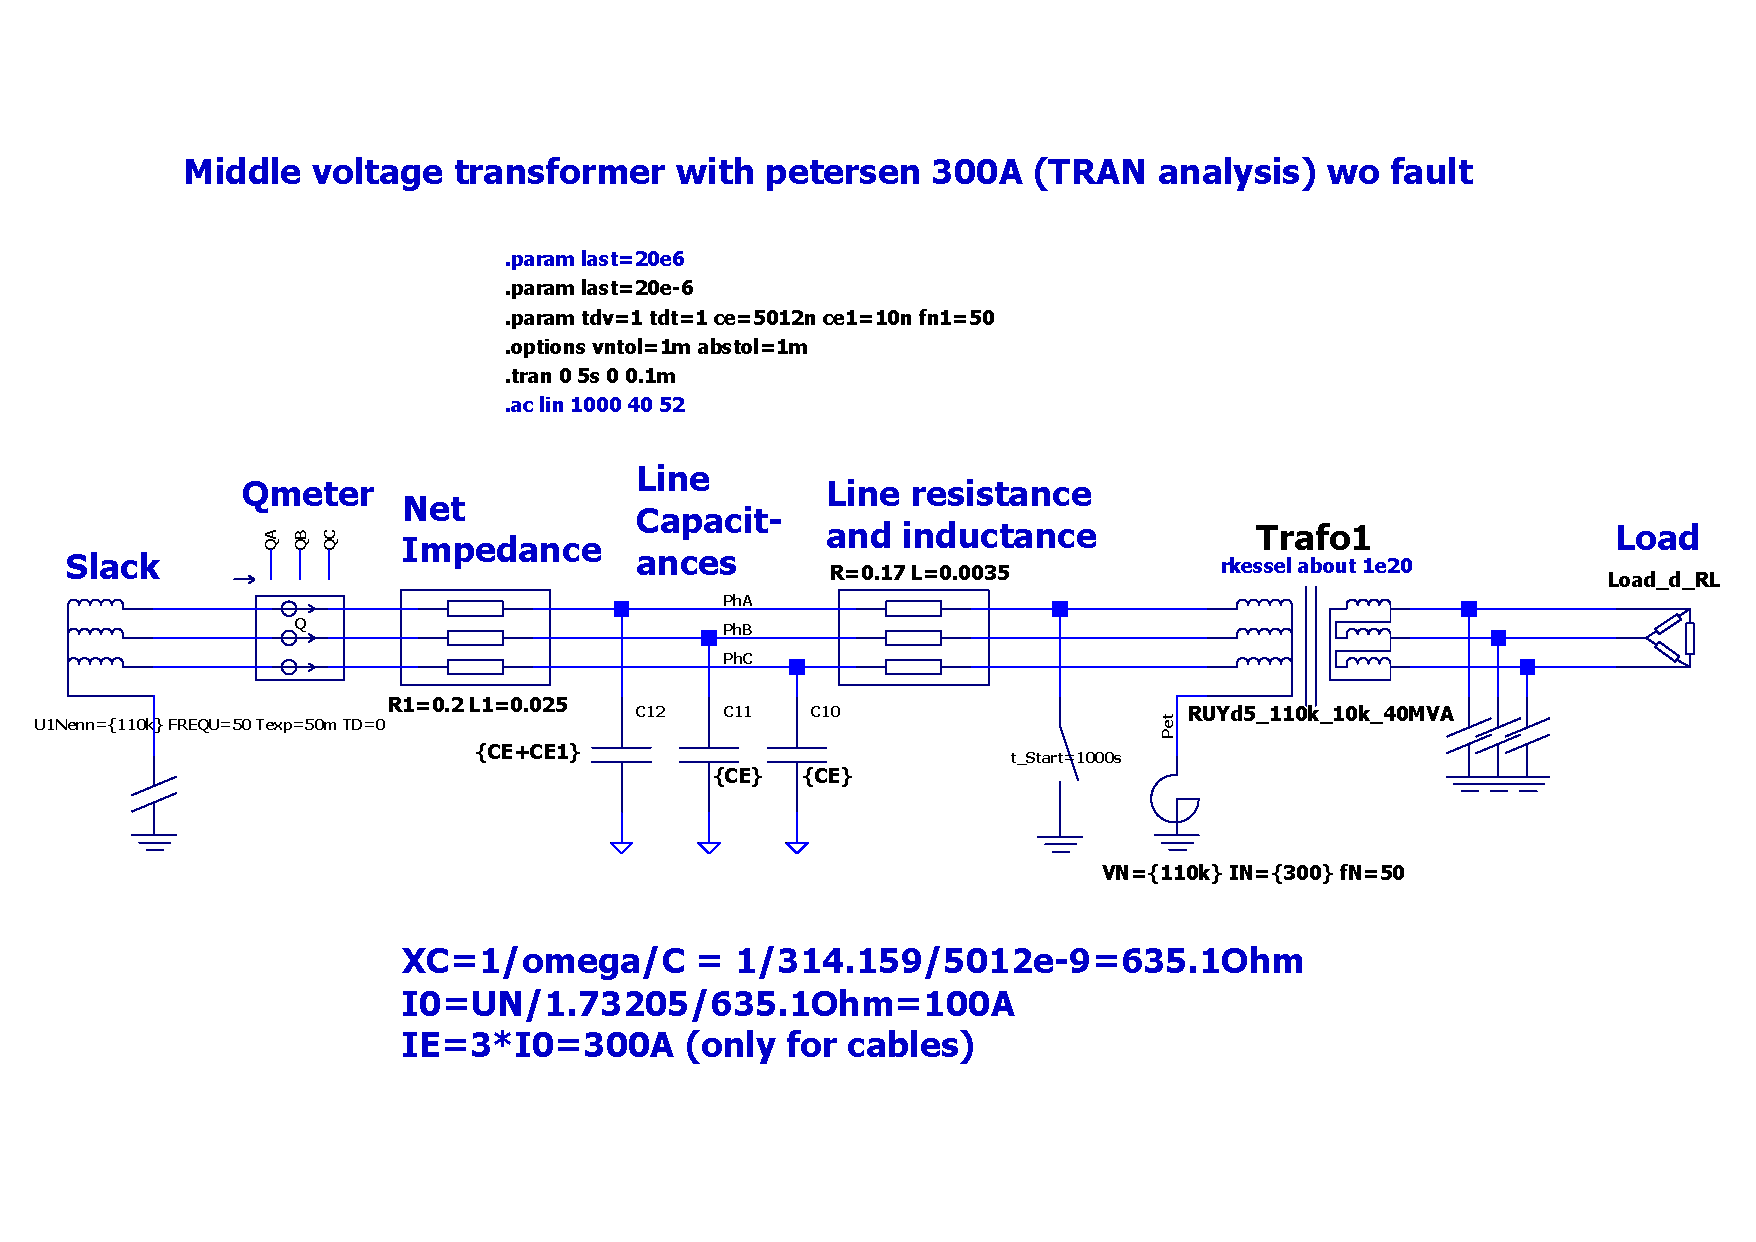
\includegraphics[width=0.90\textwidth]{figures/05_Petersen_earth_faults/Petersen_without_fault_TRAN_schematic}
	\caption{Petersen without fault - schematic}
	\label{fig:Figure1a}
\end{figure}

\begin{figure}[H]
	\centering
	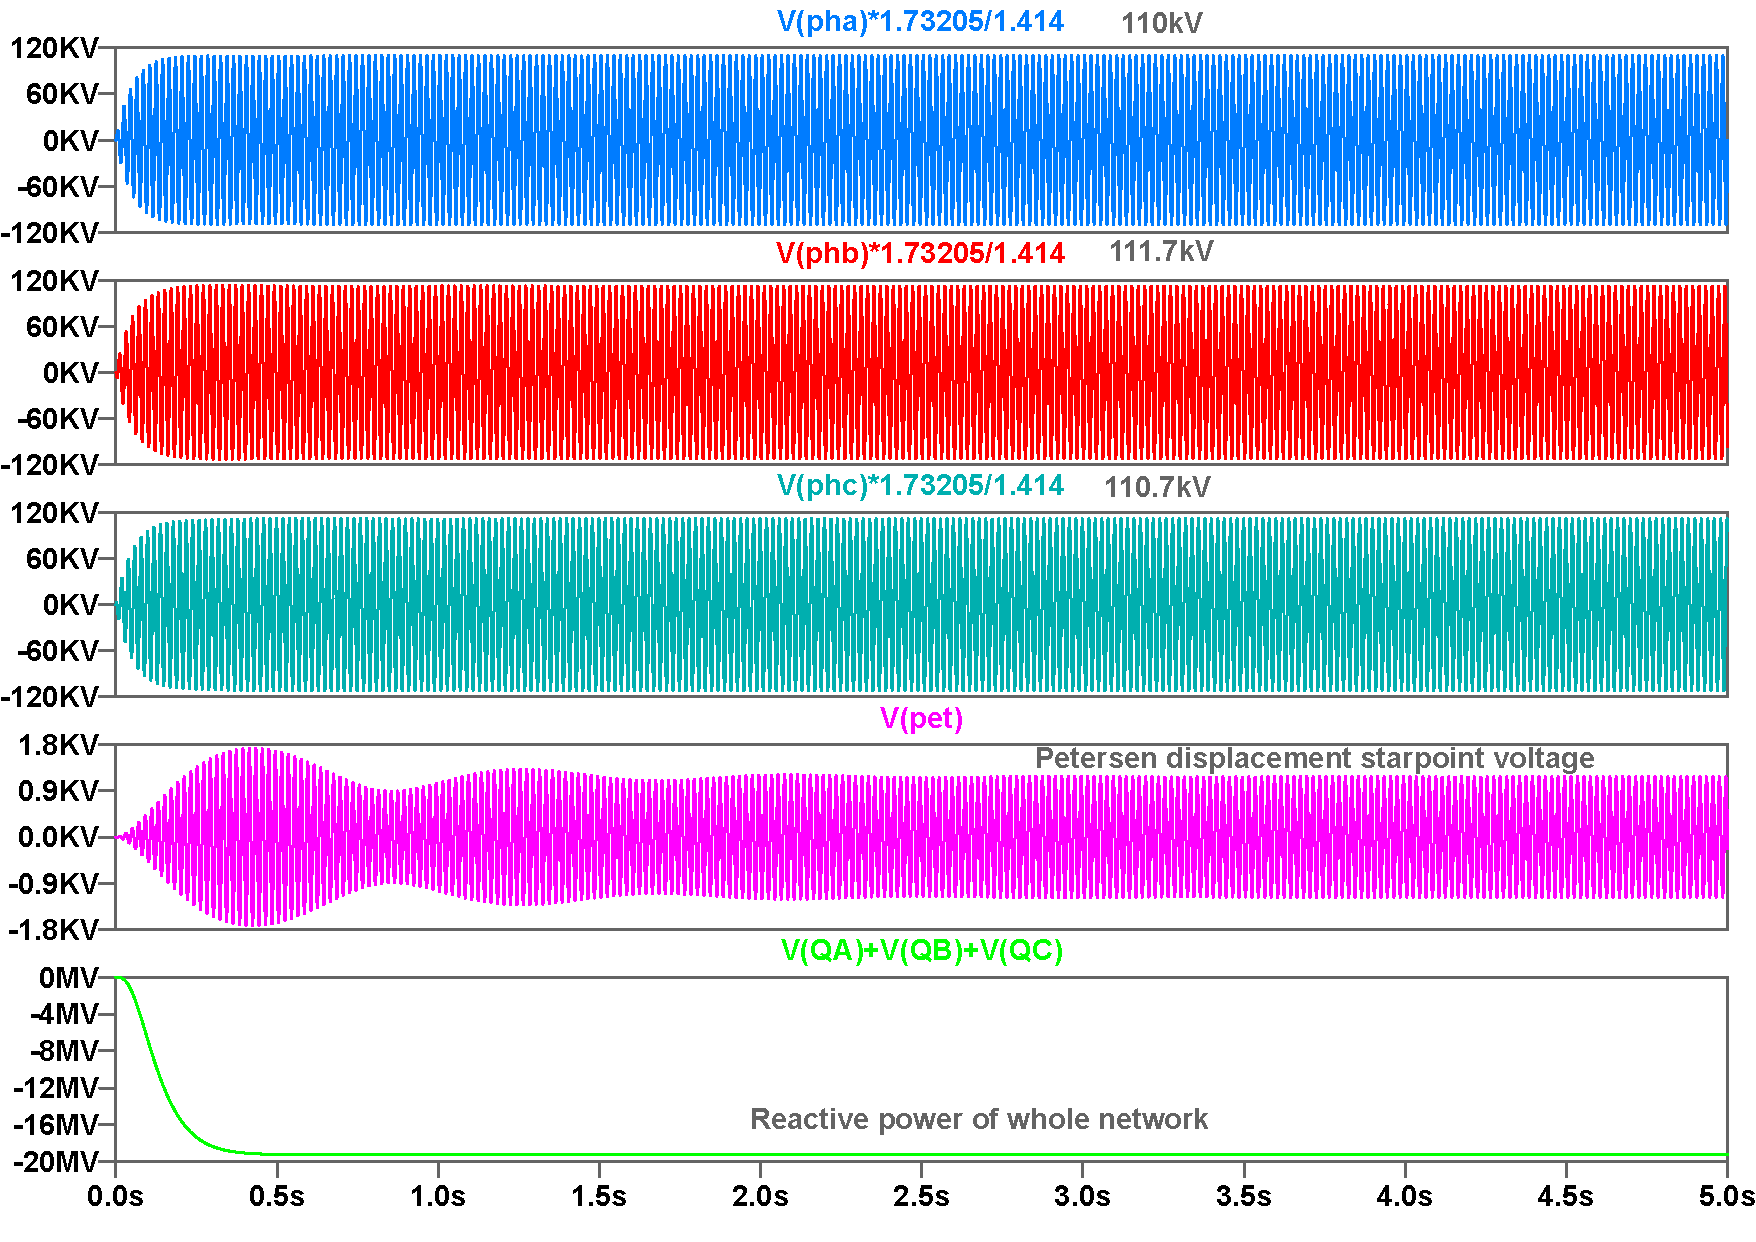
\includegraphics[width=0.90\textwidth]{figures/05_Petersen_earth_faults/Petersen_without_fault_TRAN_waveform.pdf}
	\caption{Petersen without fault TRAN - waveform}
	\label{fig:Figure1}
\end{figure}



\begin{figure}[H]
	\centering
	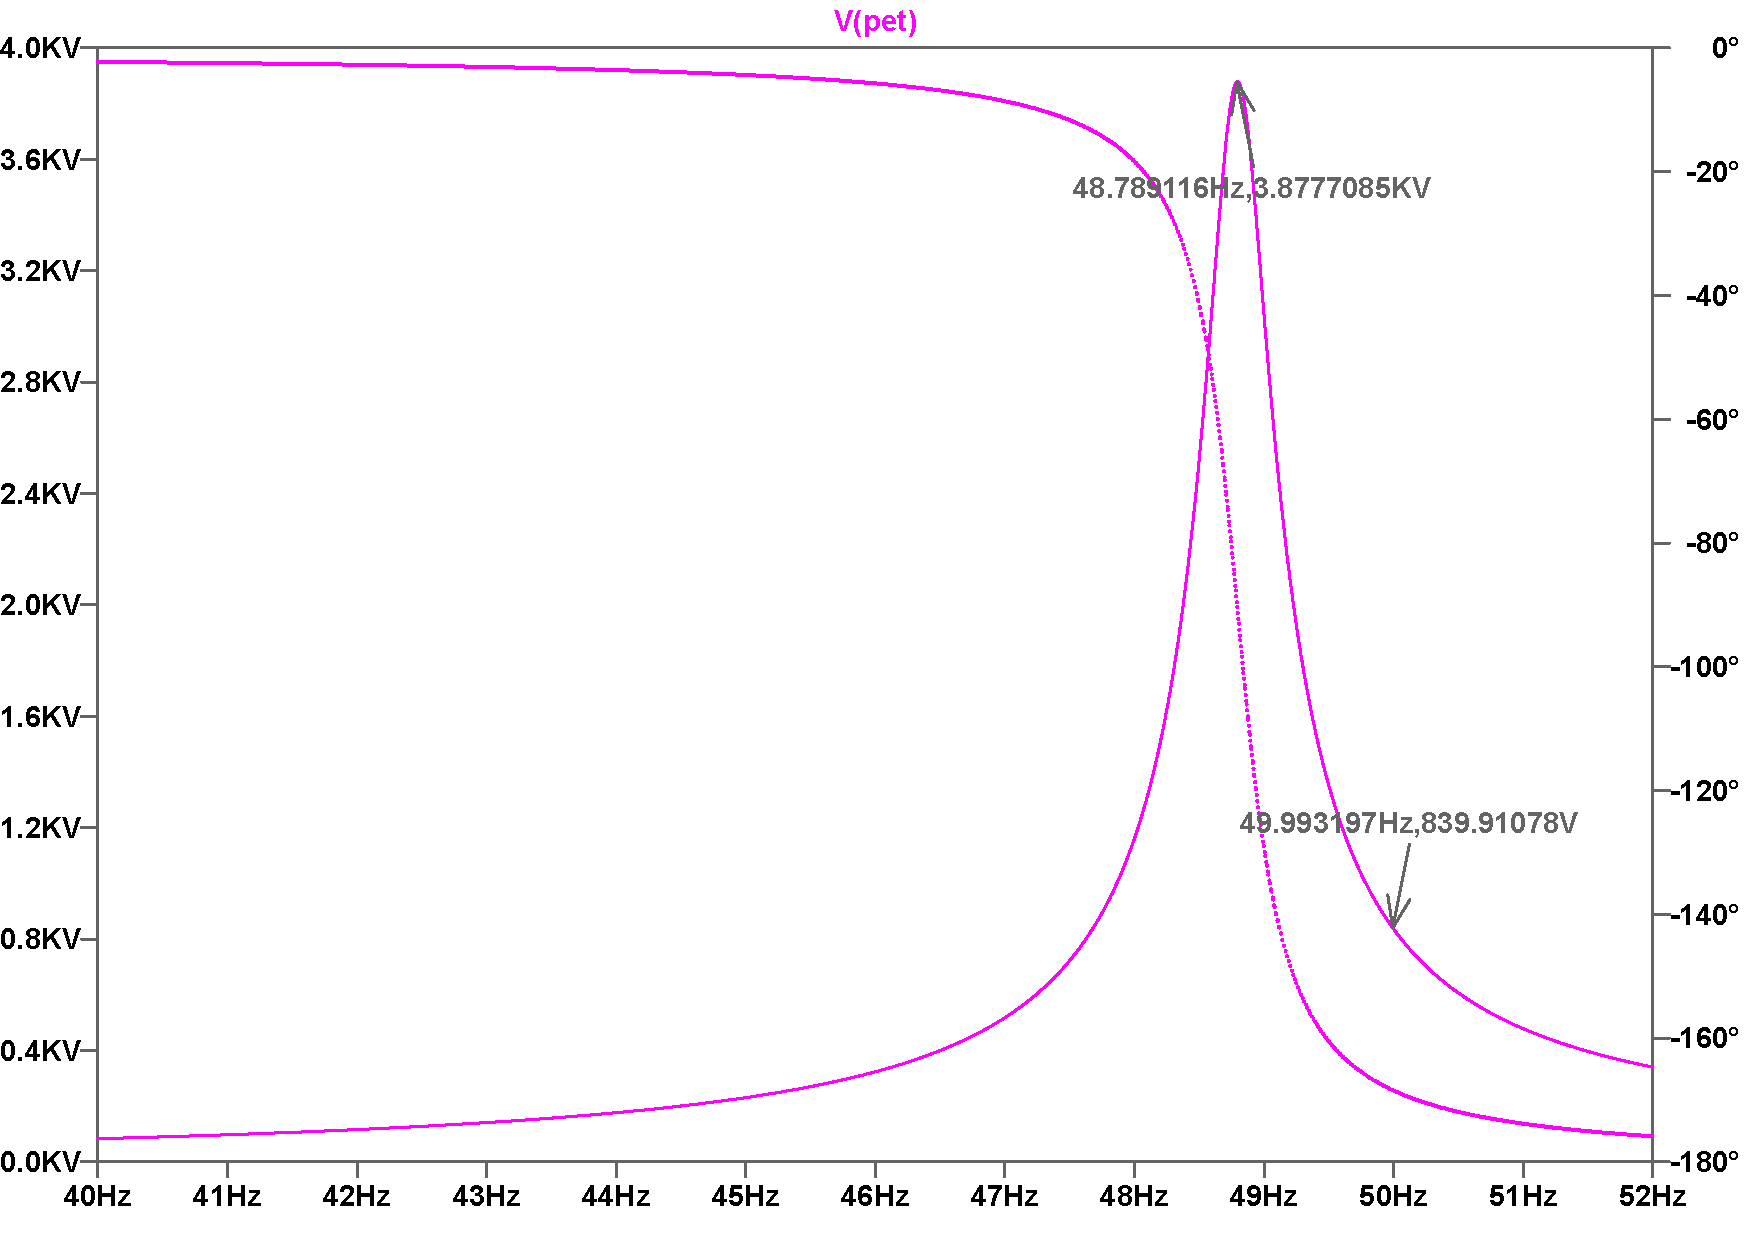
\includegraphics[width=0.90\textwidth]{figures/05_Petersen_earth_faults/Petersen_without_fault_AC_waveform.pdf}
	\caption{Petersen without fault AC starpoint (Petersen) voltage - waveform}
	\label{fig:Figure2}
\end{figure}

%\begin{figure}[H]
%	\centering
%	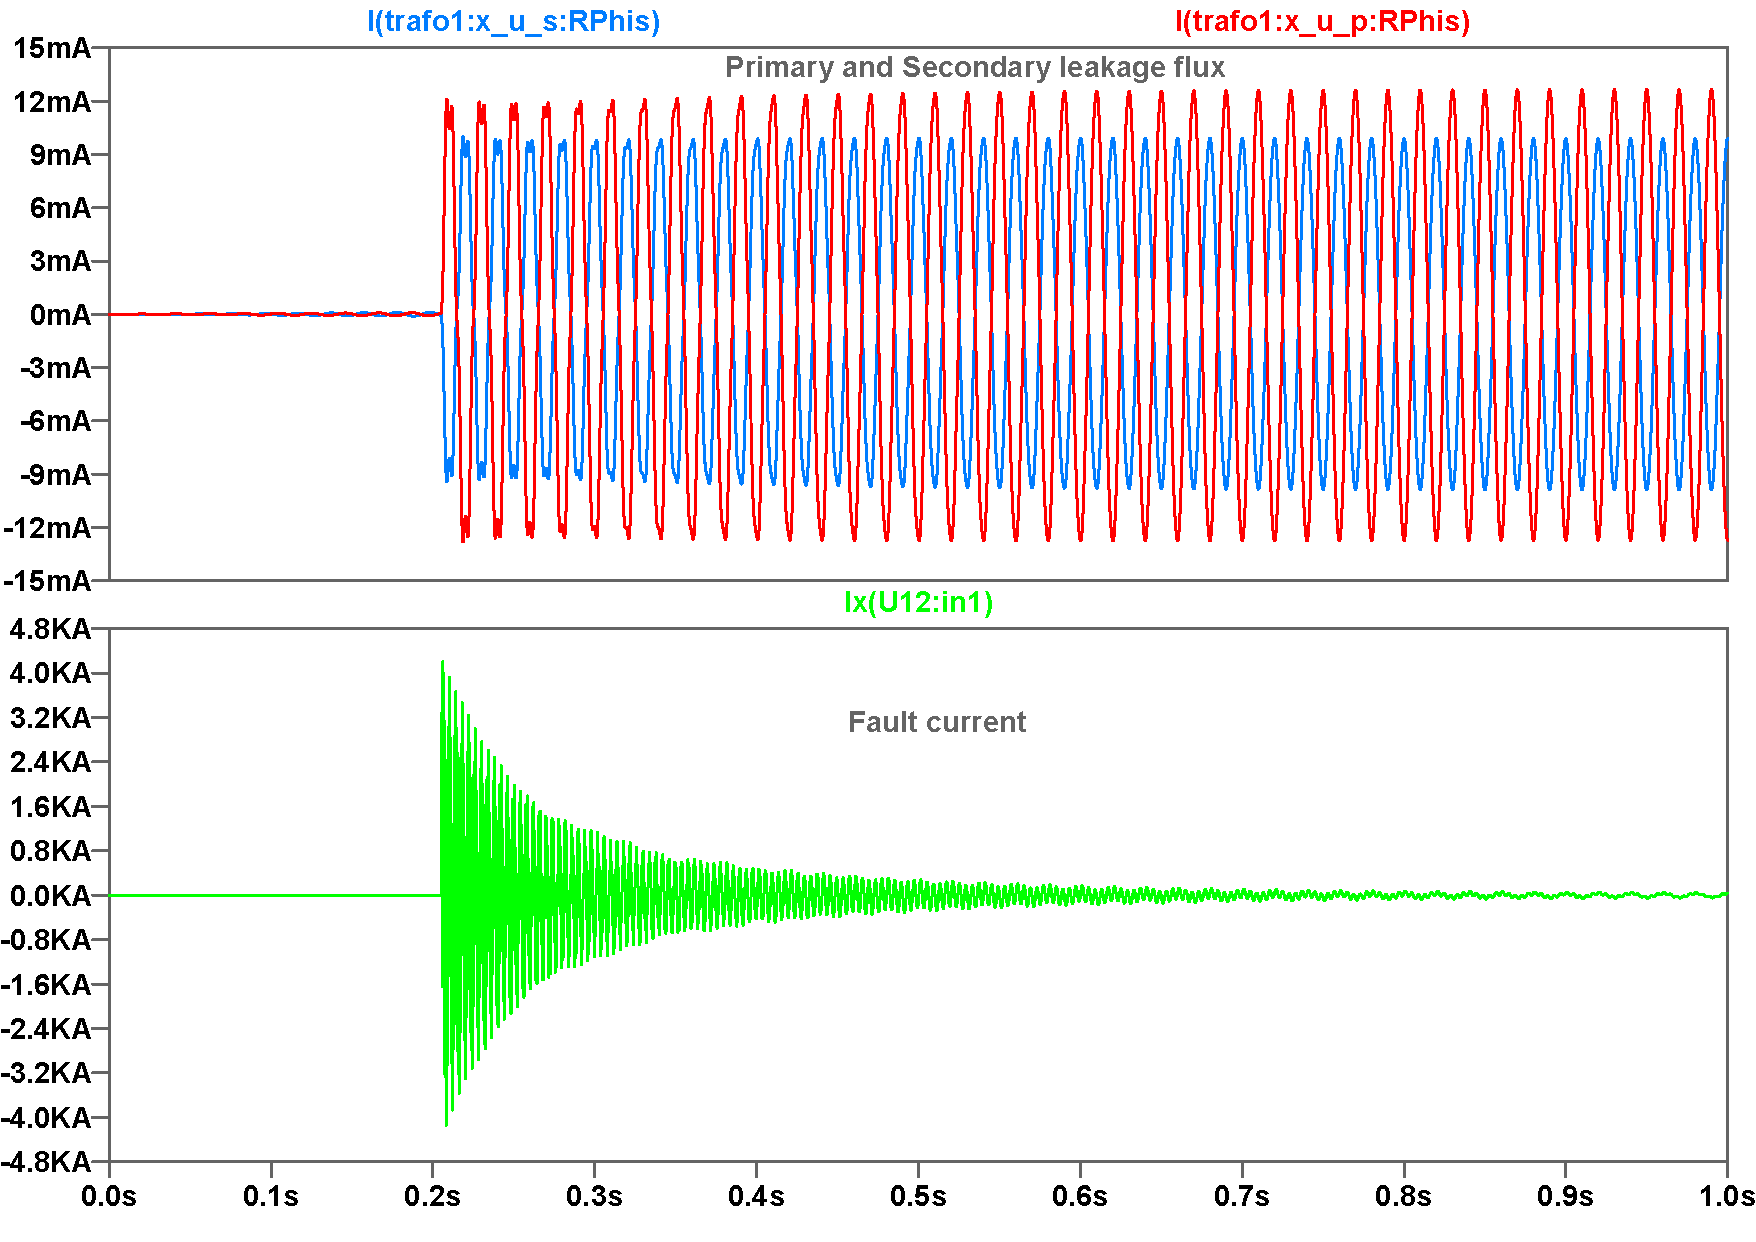
\includegraphics[width=0.90\textwidth]{figures/05_Petersen_earth_faults/Petersen_with_fault_hierarchical_model_TRAN_waveform.pdf}
%	\caption{Petersen with fault TRAN hierarchical model - waveform}
%	\label{fig:Figure3}
%\end{figure}

\begin{figure}[H]
	\centering
	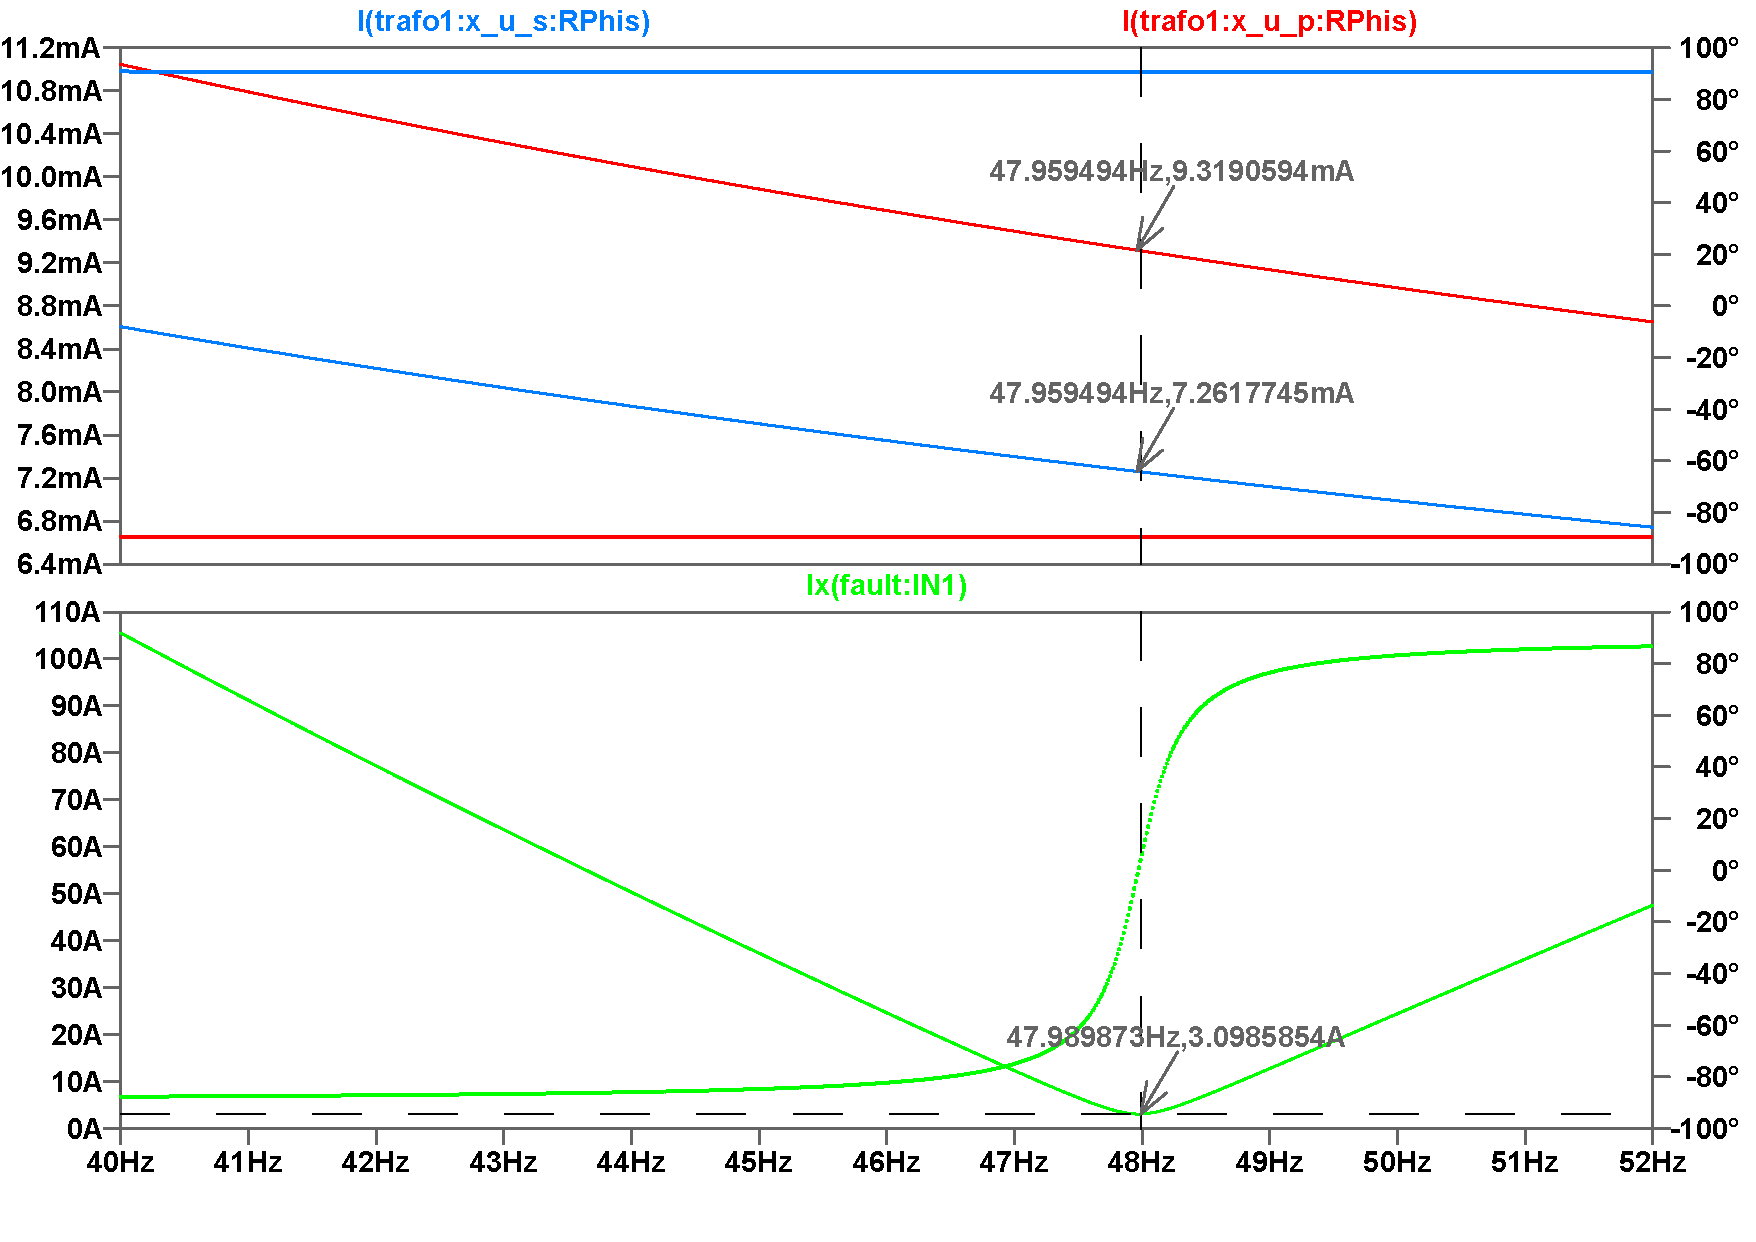
\includegraphics[width=0.90\textwidth]{figures/05_Petersen_earth_faults/Petersen_with_fault_hierarchical_model_AC_waveform.pdf}
	\caption{Petersen with fault AC hierarchical model - waveform}
	\label{fig:Figure4}
\end{figure}

\begin{figure}[H]
	\centering
	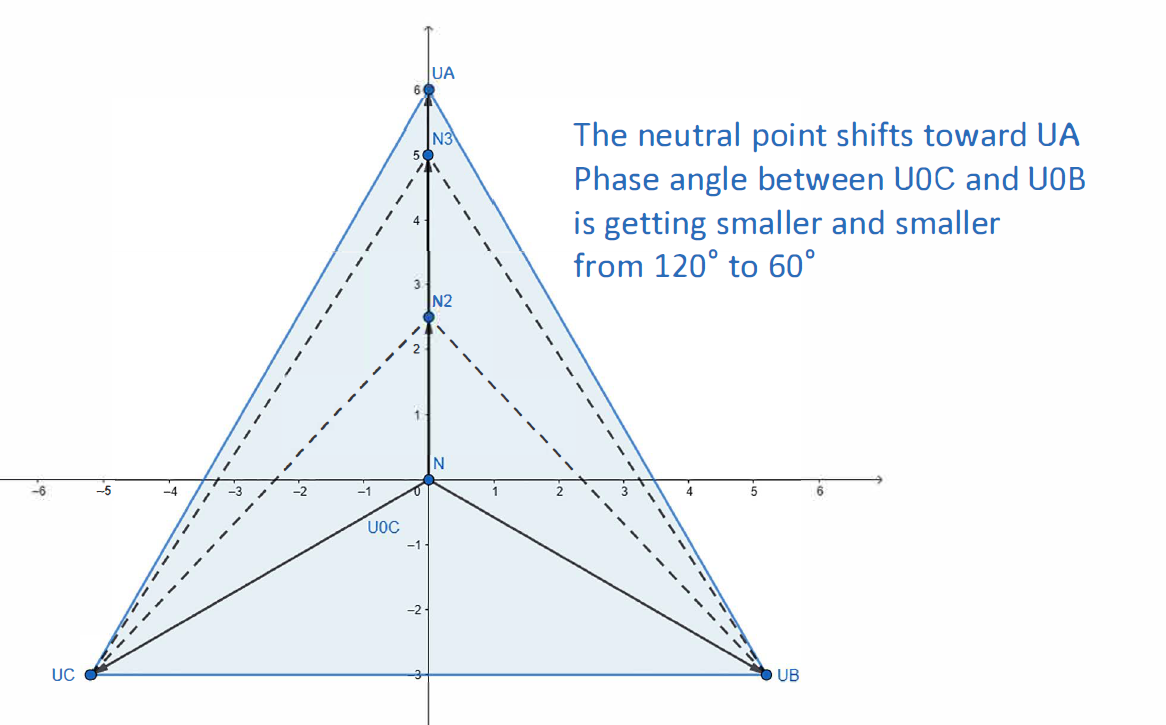
\includegraphics[width=0.90\textwidth]{figures/05_Petersen_earth_faults/Starpoint_Geogebra.png}
	\caption{Principal phase difference between the voltages U0B and U0C in fault case, plotted with GeoGebra - see file Starpoint\_vektor.ggb}
	\label{fig:FigureX}
\end{figure}

%\begin{figure}[H]
%	\centering
%	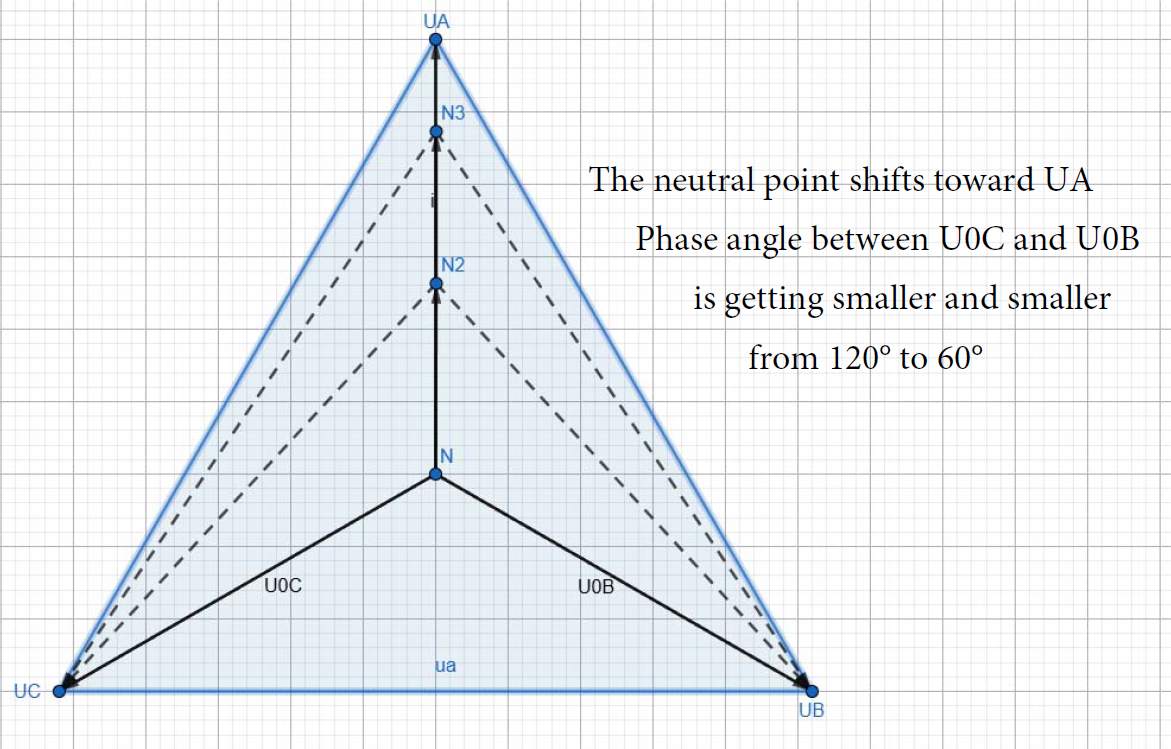
\includegraphics[width=0.90\textwidth]{figures/05_Petersen_earth_faults/Geogebra_Petersen.png}
%	\caption{Phasedifference of the phase voltages U0B,U0C drawn with GeoGebra}
%	\label{fig:FigureX}
%\end{figure}

\begin{figure}[H]
	\centering
	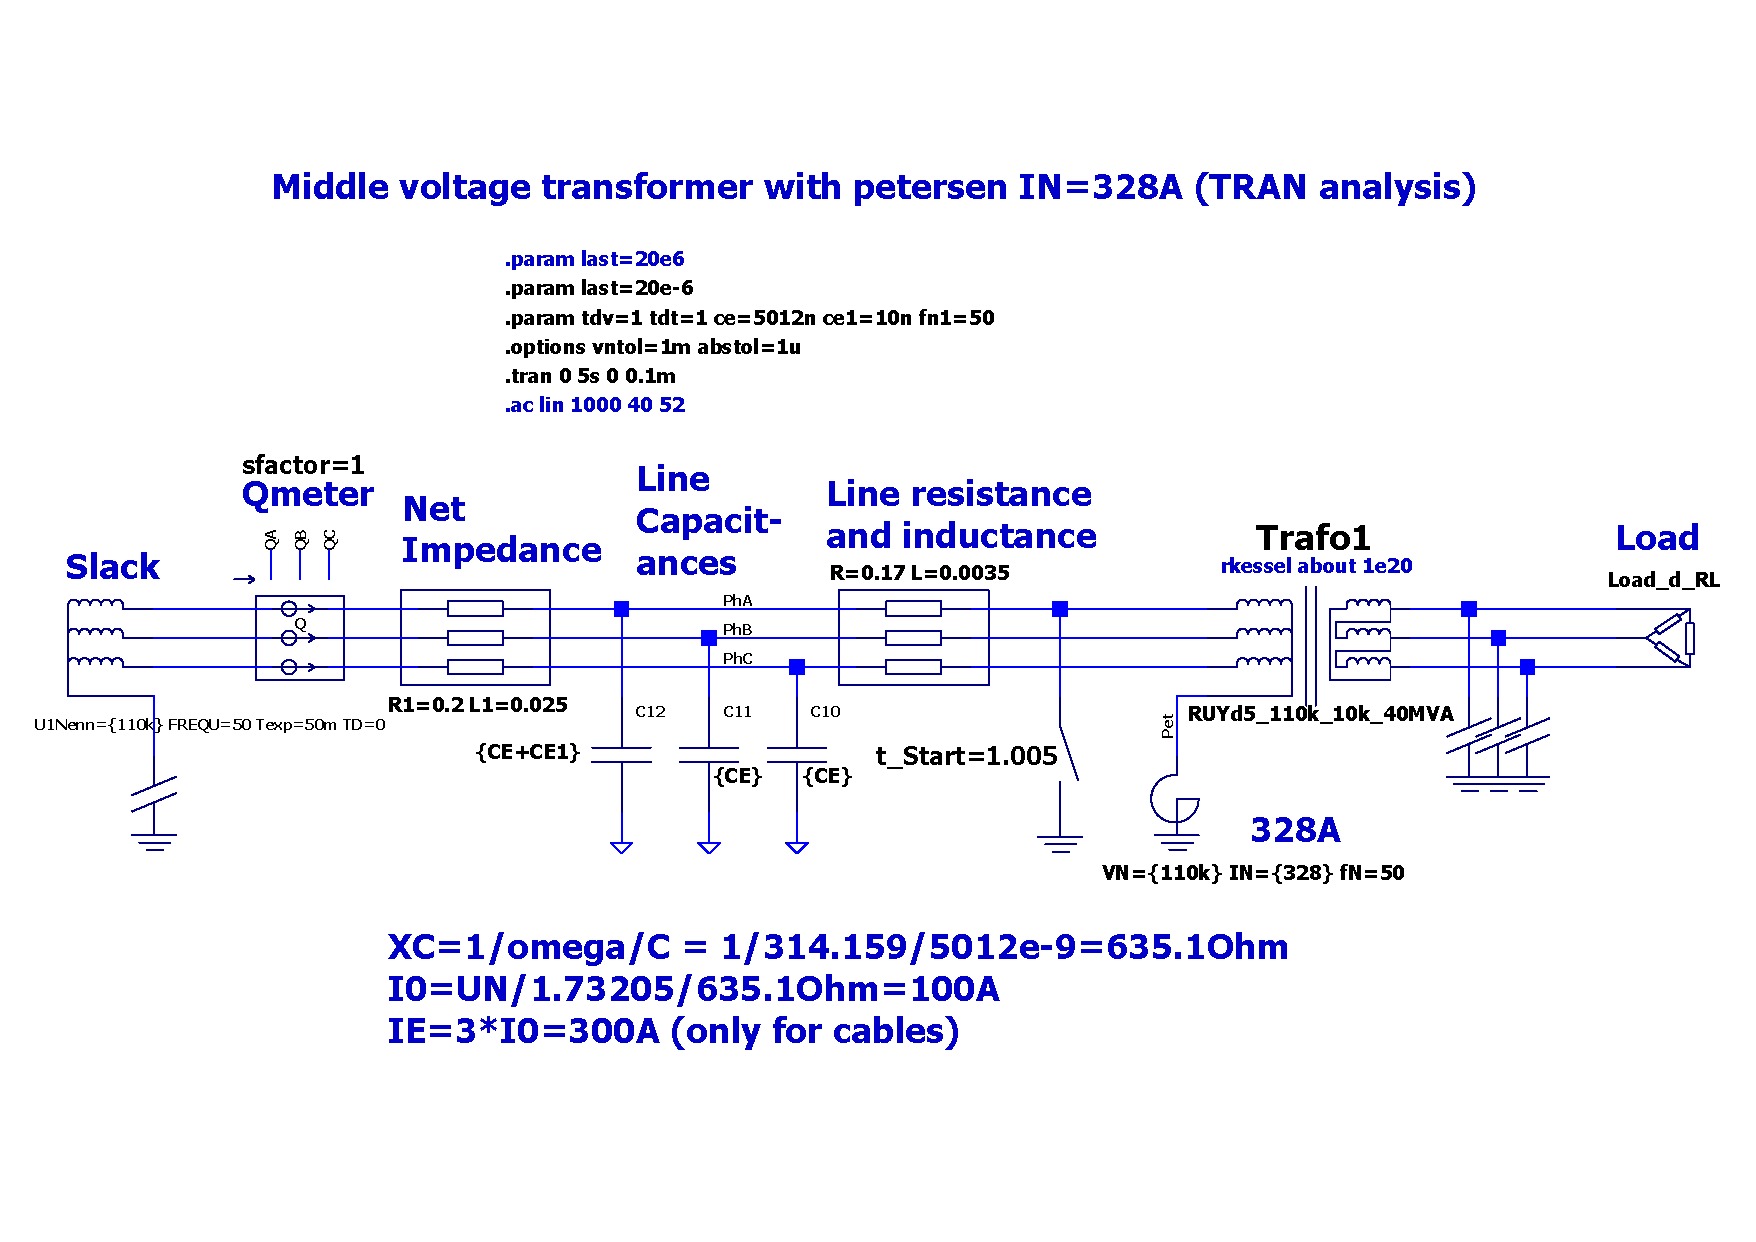
\includegraphics[width=0.90\textwidth]{figures/05_Petersen_earth_faults/Petersen_with_fault_TRAN_schematic.pdf}
	\caption{Petersen with fault TRAN - schematic}
	\label{fig:Figure5a}
\end{figure}

\begin{figure}[H]
	\centering
	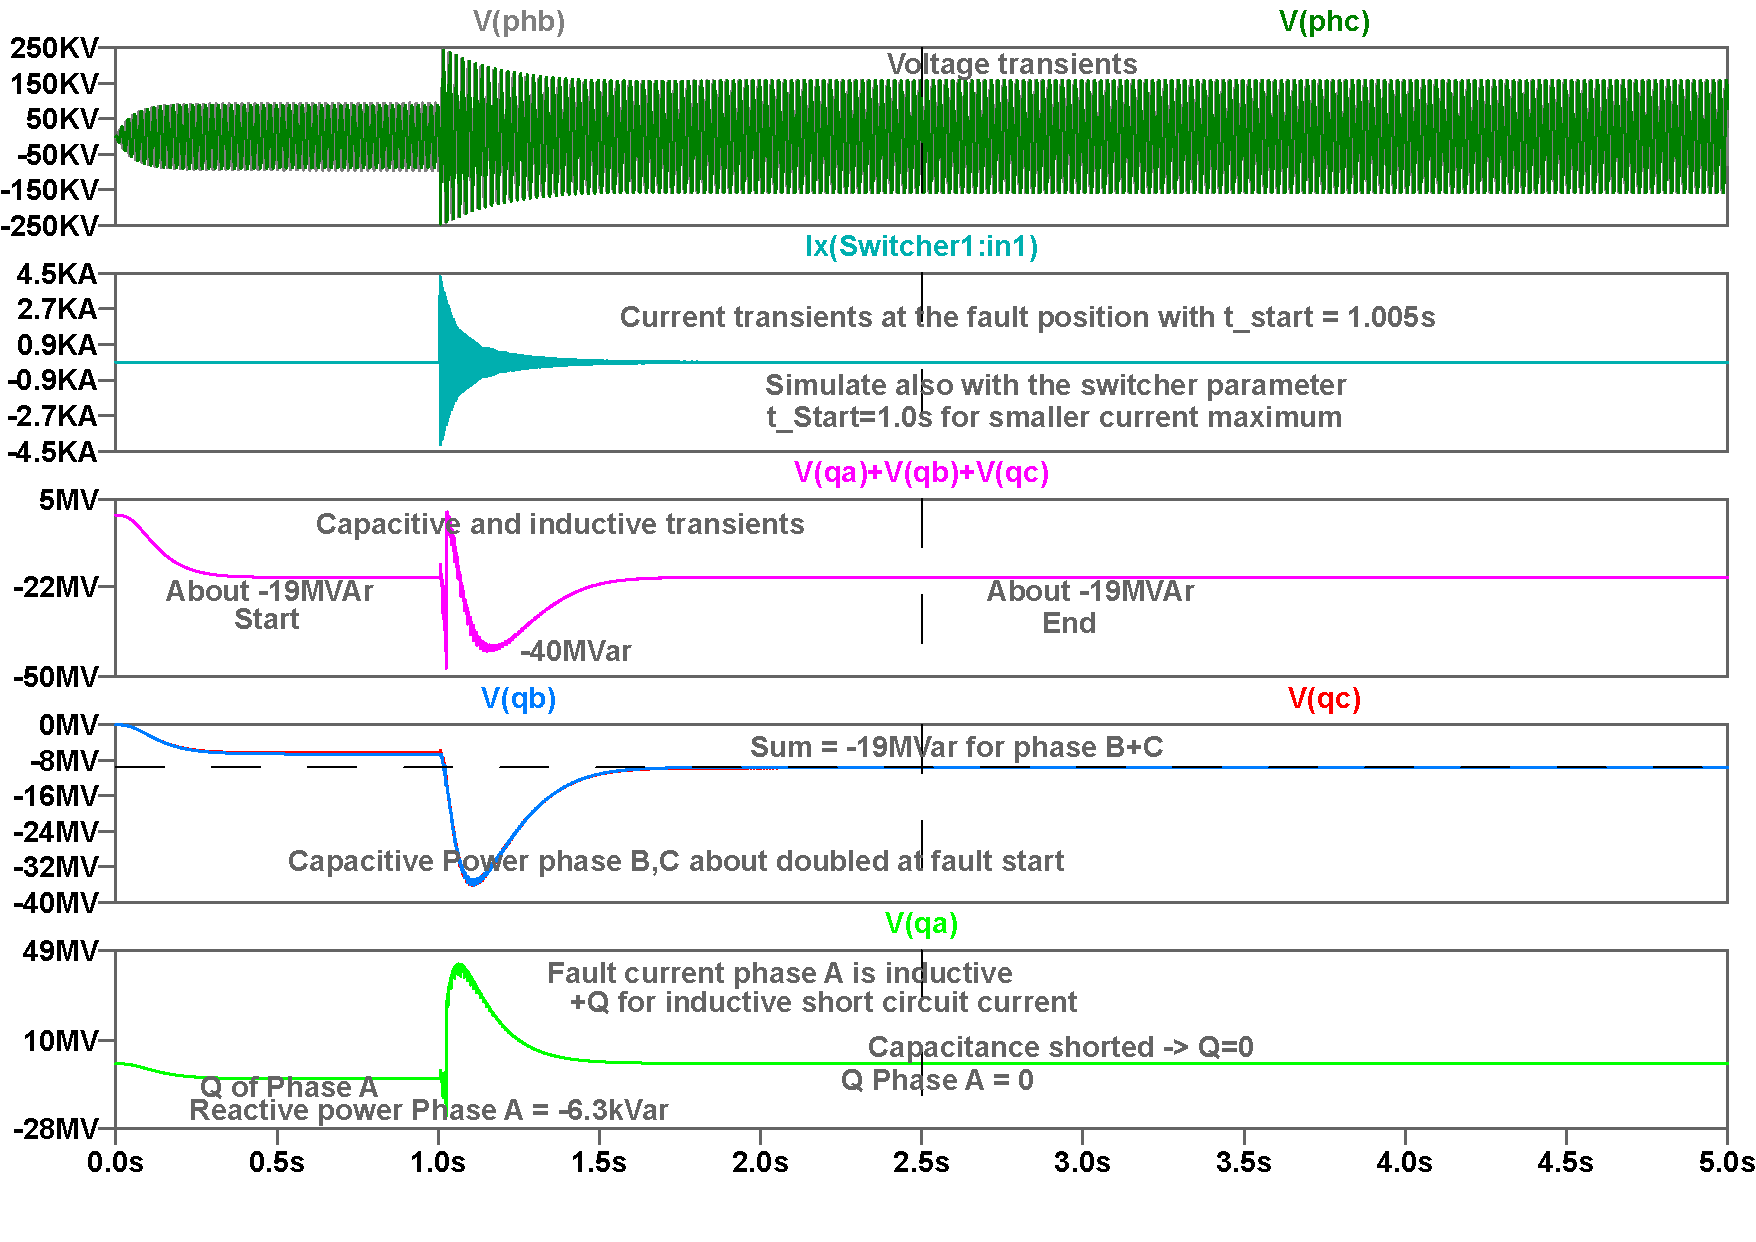
\includegraphics[width=0.90\textwidth]{figures/05_Petersen_earth_faults/Petersen_with_fault_TRAN_waveform.pdf}
	\caption{Petersen with fault TRAN - waveform}
	\label{fig:Figure5}
\end{figure}

\begin{figure}[H]
	\centering
	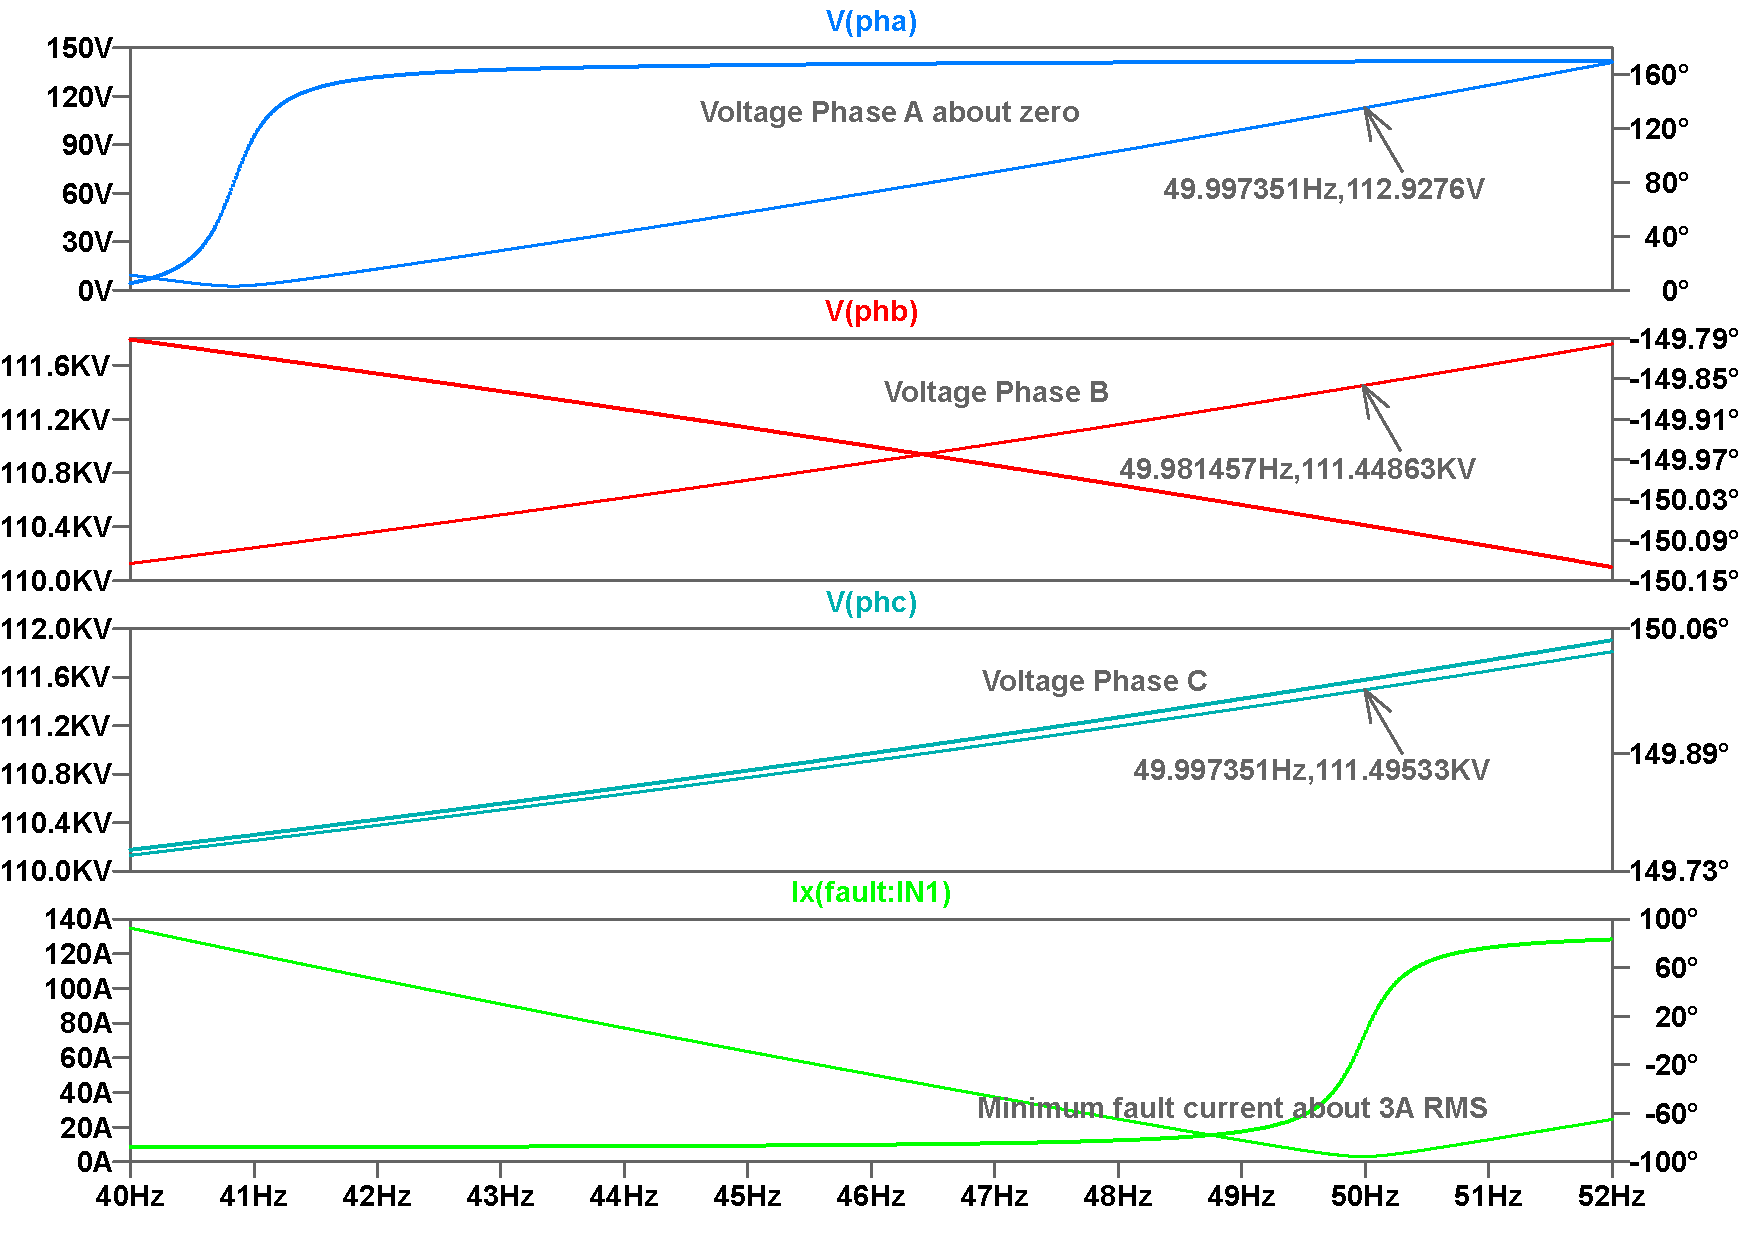
\includegraphics[width=0.90\textwidth]{figures/05_Petersen_earth_faults/Petersen_with_fault_AC_waveform.pdf}
	\caption{Petersen with fault AC - waveform}
	\label{fig:Figure6}
\end{figure}




\begin{figure}[H]
	\centering
	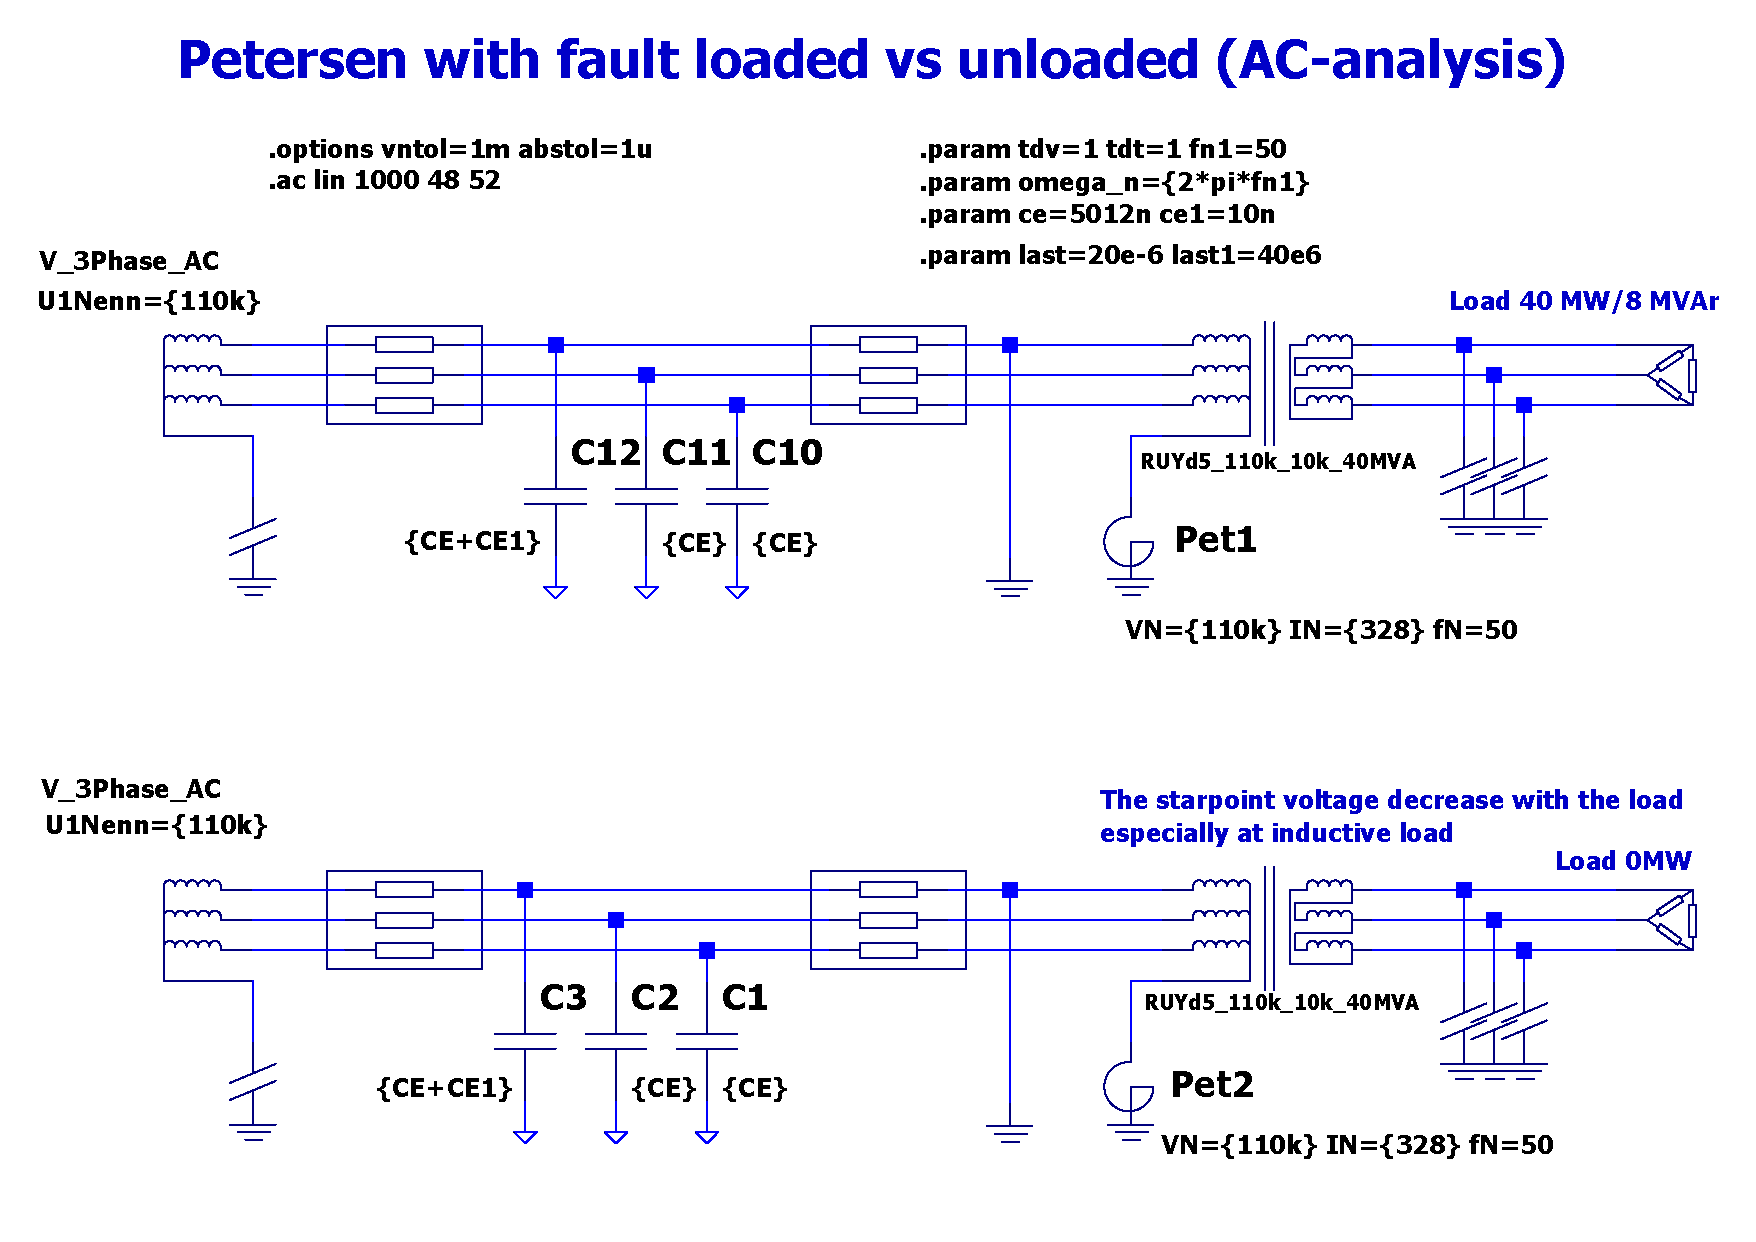
\includegraphics[width=0.90\textwidth]{figures/05_Petersen_earth_faults/Petersen_with_fault_with_load_vs_without_load_AC_schematic.pdf}
	\caption{Petersen with fault and load AC - schematic}
	\label{fig:Figure7a}
\end{figure}

\begin{figure}[H]
	\centering
	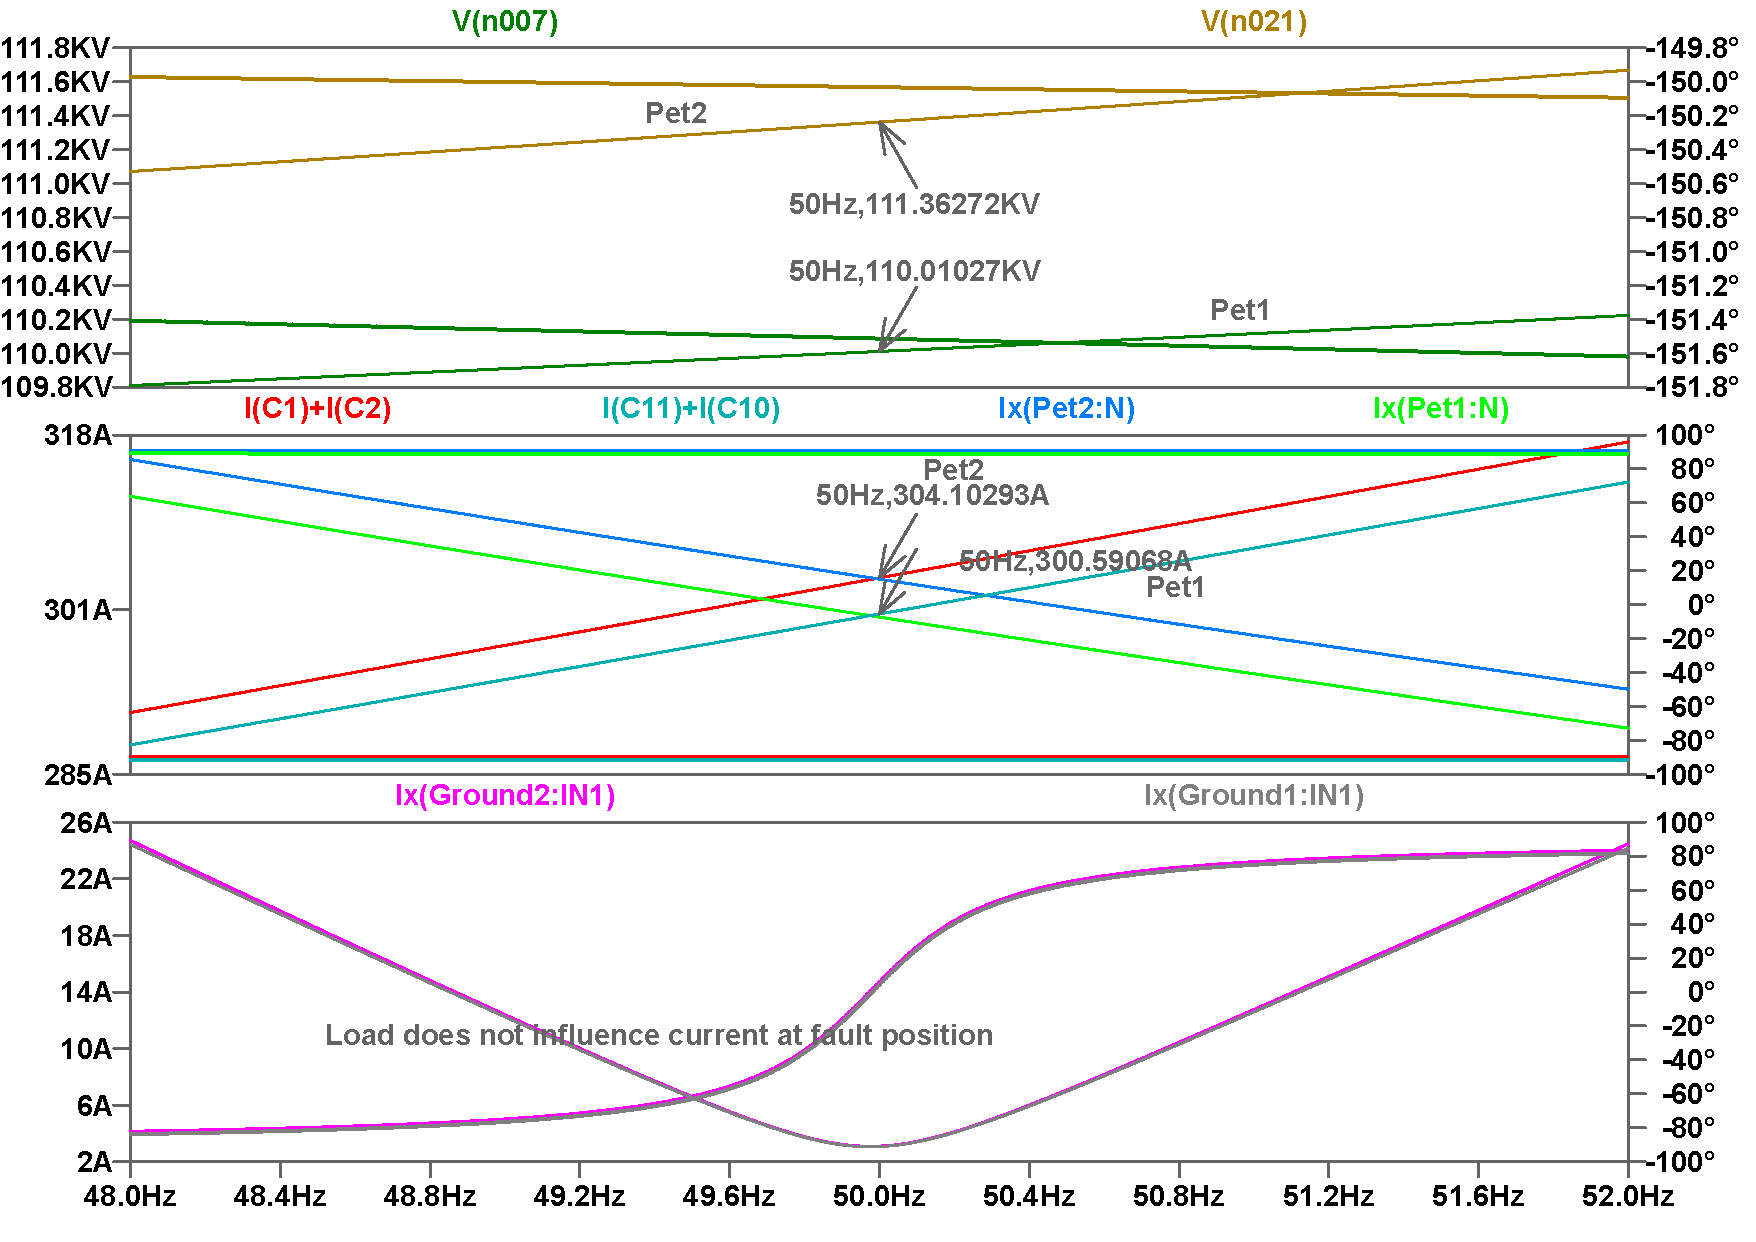
\includegraphics[width=0.90\textwidth]{figures/05_Petersen_earth_faults/Petersen_with_fault_with_load_vs_without_load_AC_waveform.pdf}
	\caption{Petersen with fault and load AC - waveform}
	\label{fig:Figure7}
\end{figure}

\begin{figure}[H]
	\centering
	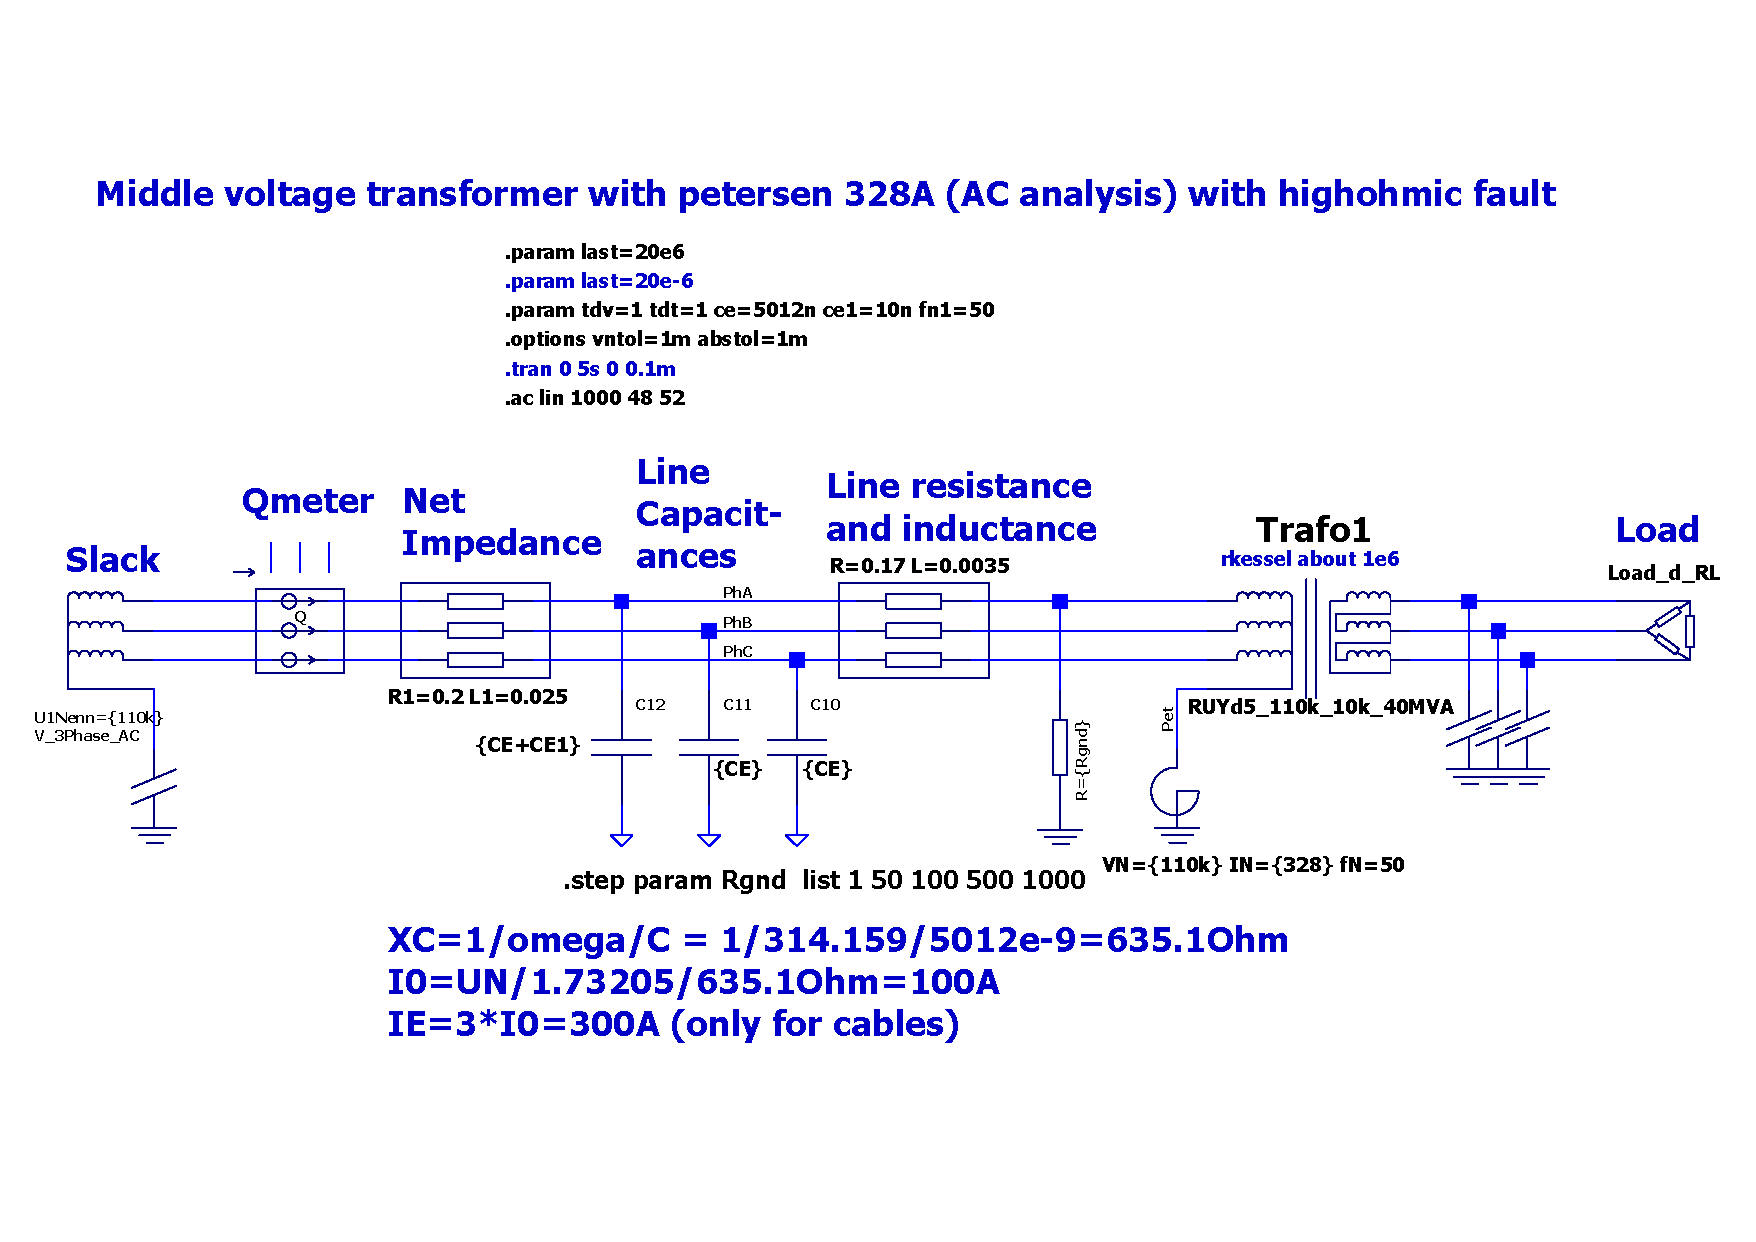
\includegraphics[width=0.90\textwidth]{figures/05_Petersen_earth_faults/Petersen_with_fault_Highohmic_AC_schematic.pdf}
	\caption{Petersen with high-resistance earth fault fault AC - schematic}
	\label{fig:Figure8a}
\end{figure}

\begin{figure}[H]
	\centering
	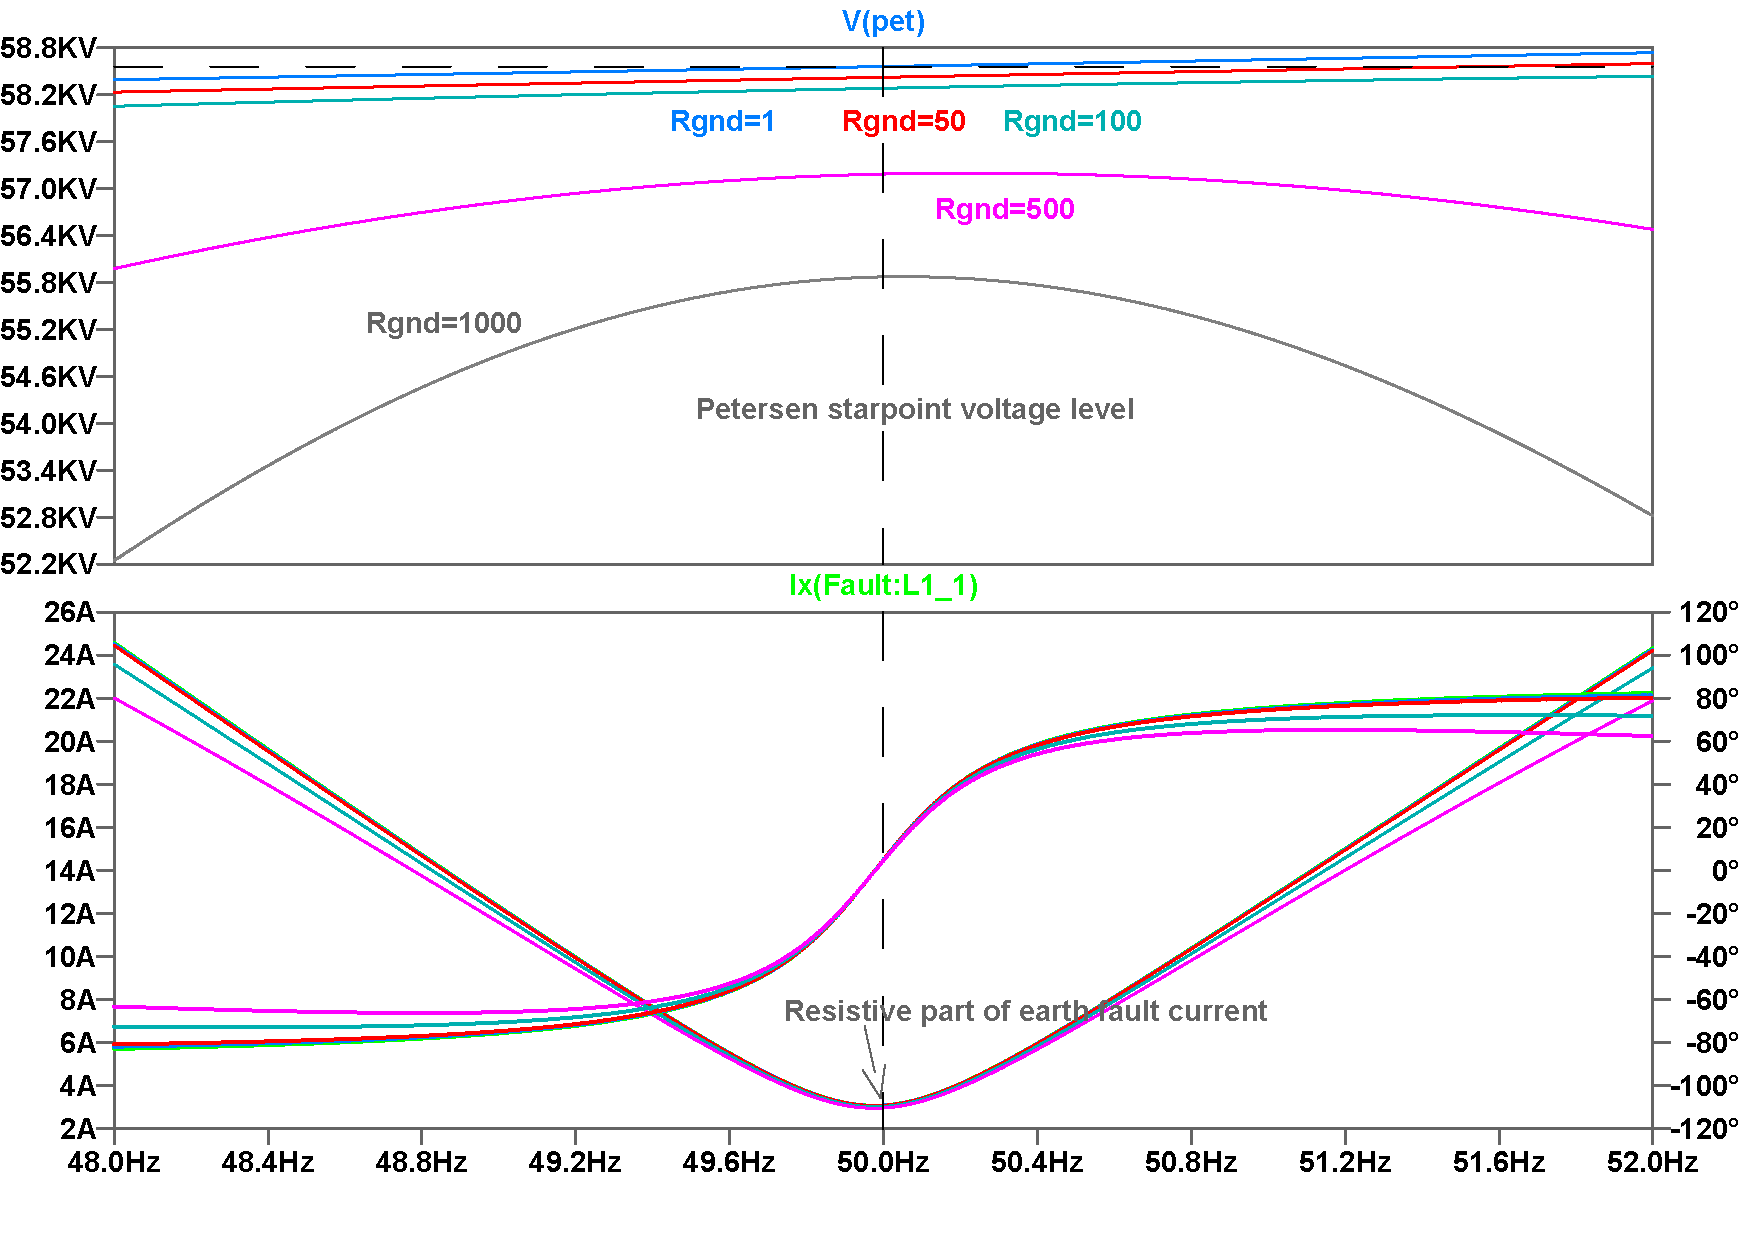
\includegraphics[width=0.90\textwidth]{figures/05_Petersen_earth_faults/Petersen_with_fault_Highohmic_AC_waveform.pdf}
	\caption{Petersen with high-resistance earth fault fault AC - waveform}
	\label{fig:Figure8}
\end{figure}

\begin{figure}[H]
	\centering
	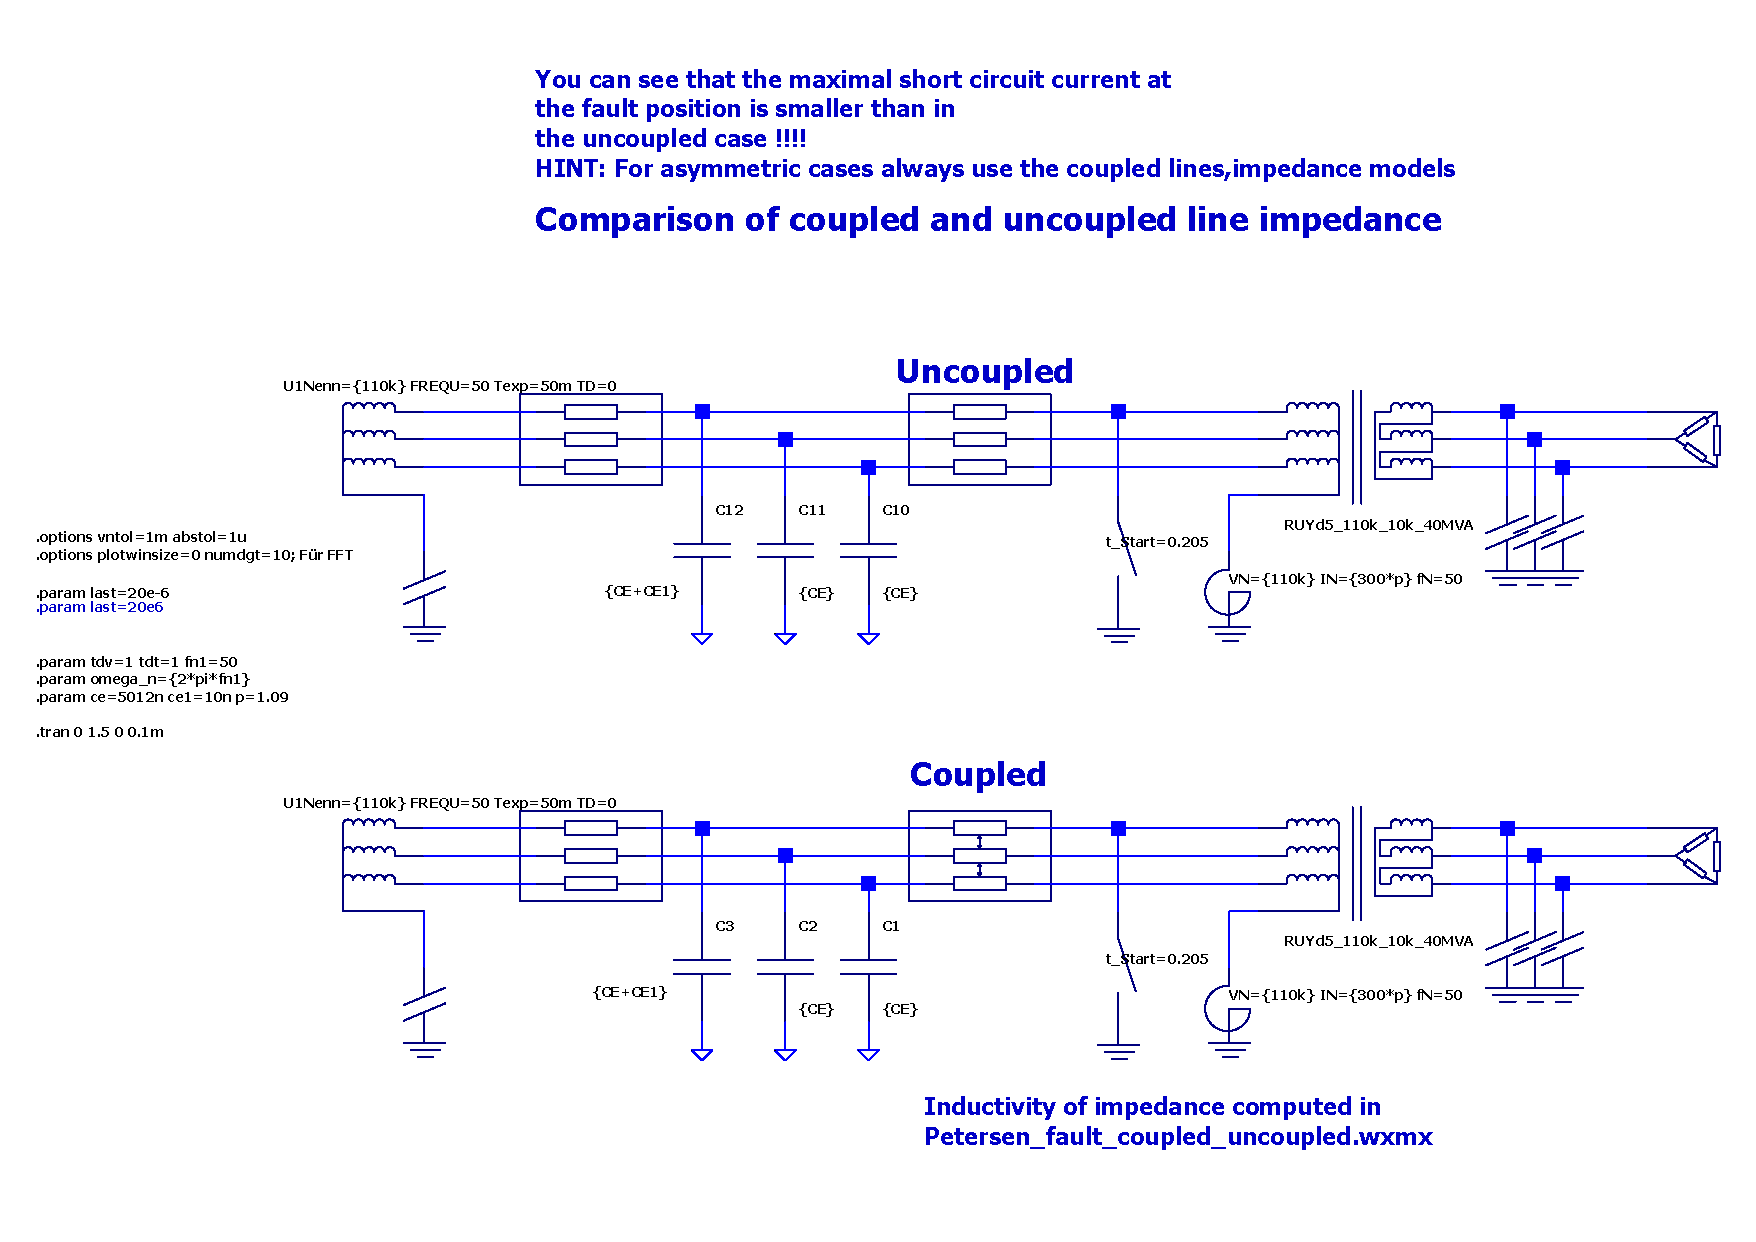
\includegraphics[width=0.90\textwidth]{figures/05_Petersen_earth_faults/Petersen_fault_coupled_uncoupled_schematic.pdf}
	\caption{Petersen with coupled and uncoupled line impedance - schematic}
	\label{fig:Figure9a}
\end{figure}

\begin{figure}[H]
	\centering
	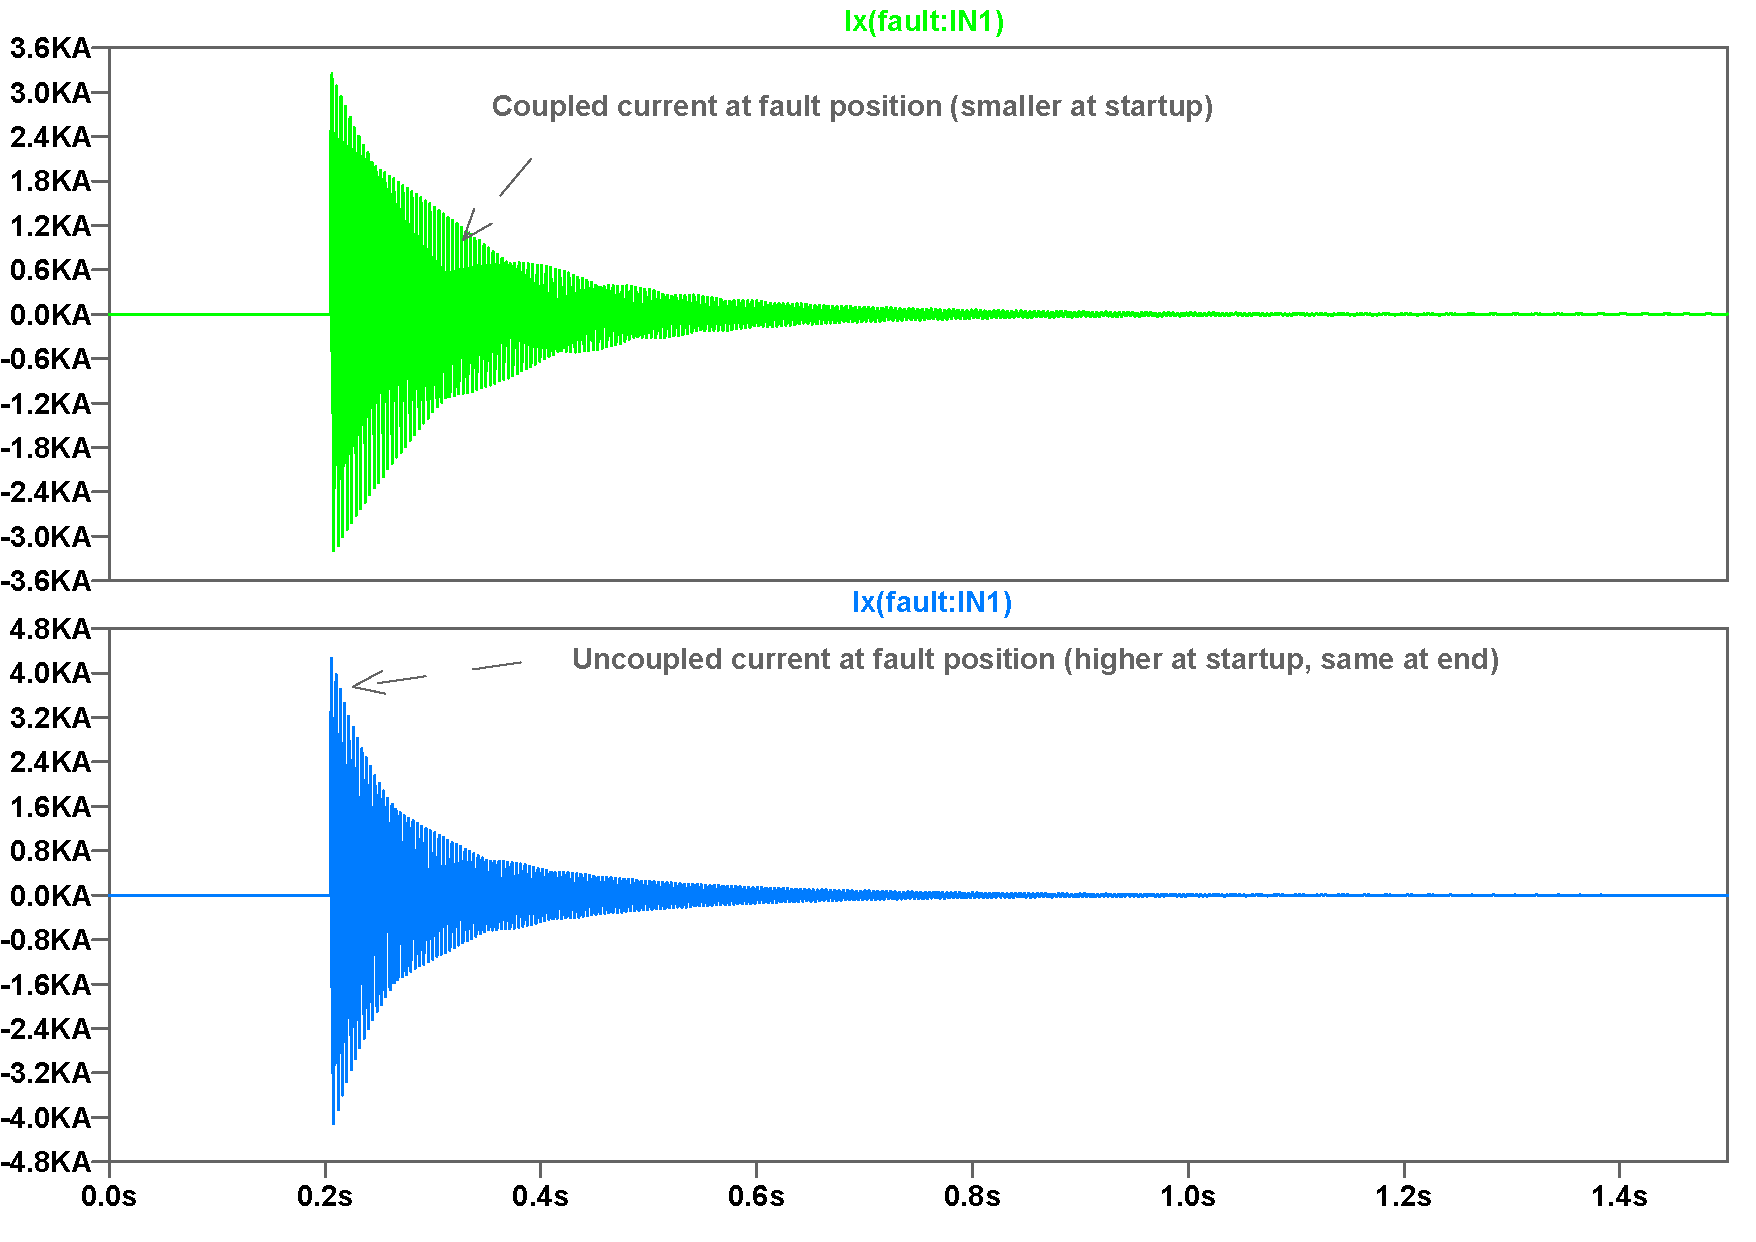
\includegraphics[width=0.90\textwidth]{figures/05_Petersen_earth_faults/Petersen_fault_coupled_uncoupled_waveform.pdf}
	\caption{Petersen with coupled and uncoupled line impedance - waveform}
	\label{fig:Figure9}
\end{figure}

\begin{figure}[H]
	\centering
	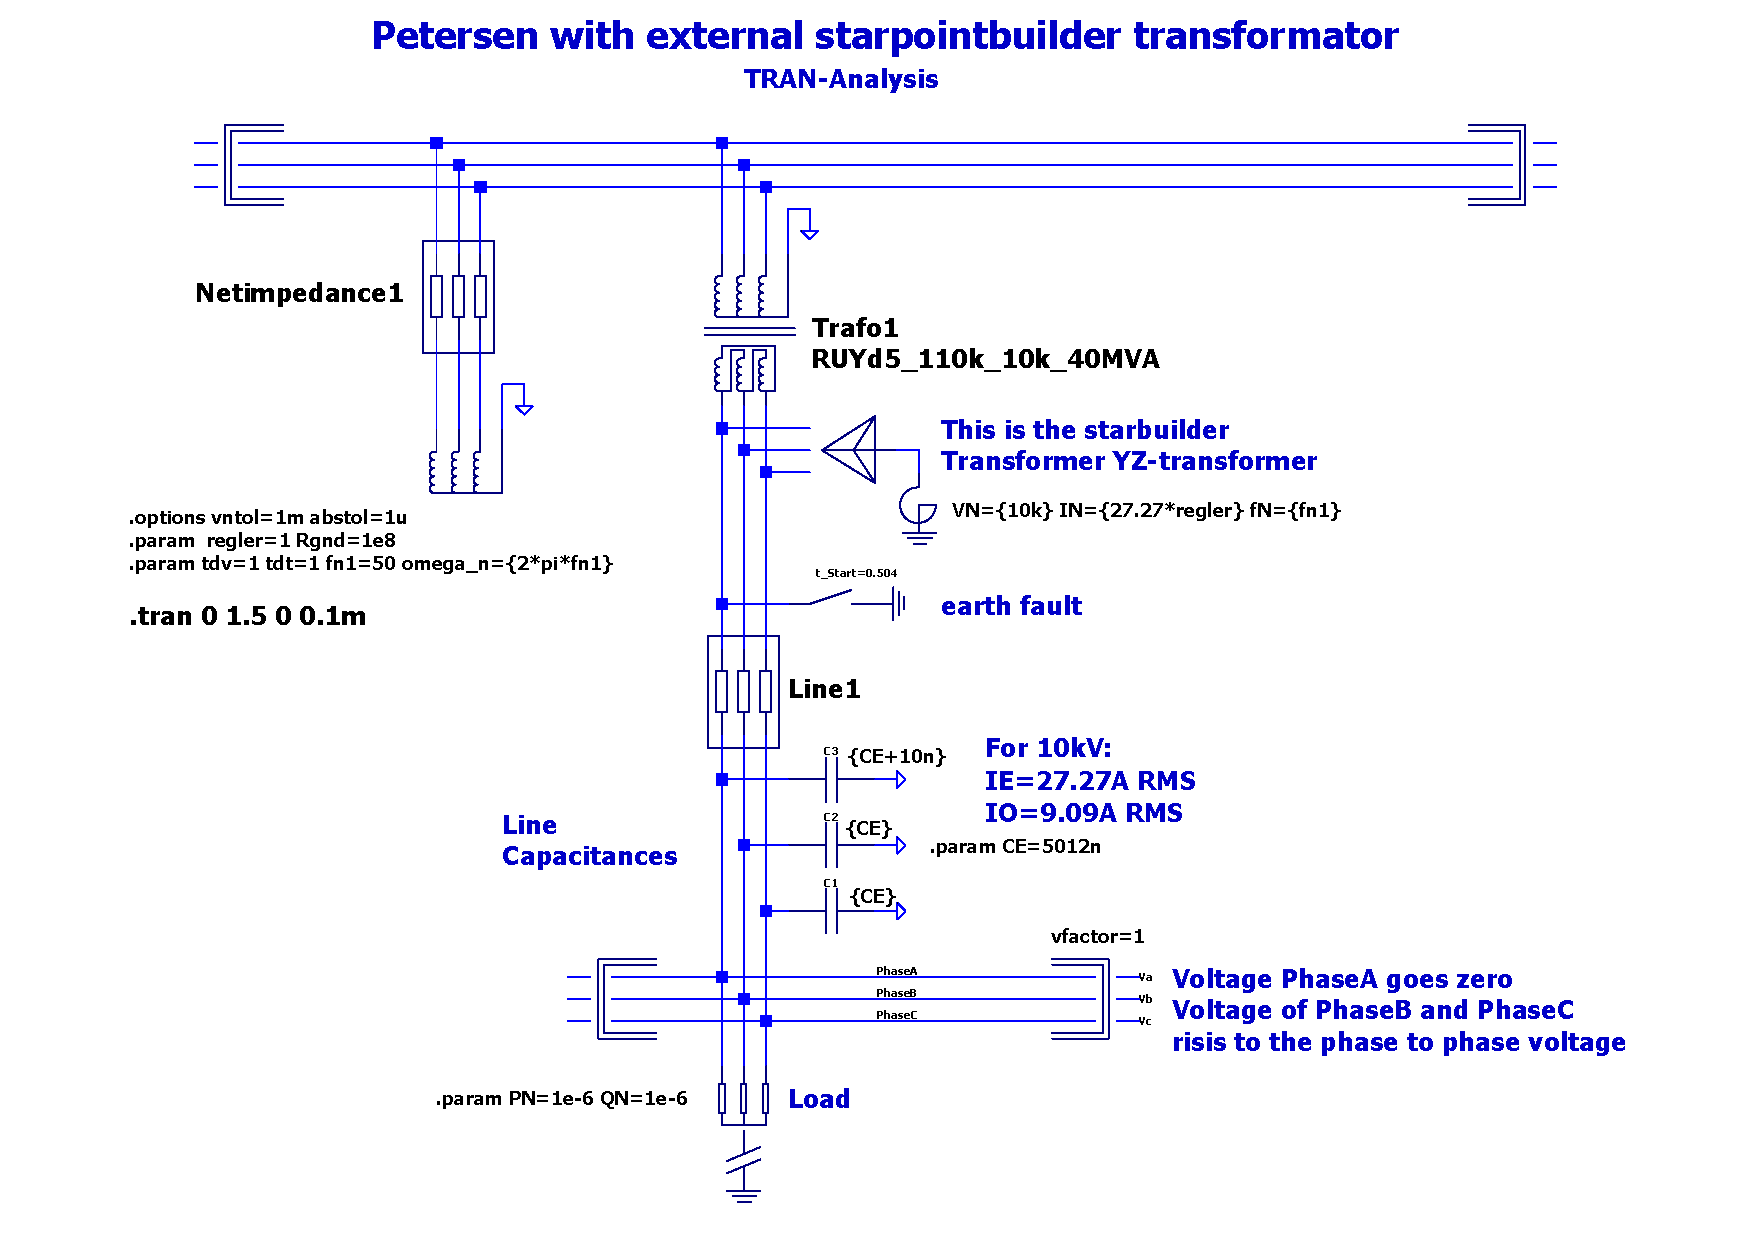
\includegraphics[width=0.90\textwidth]{figures/05_Petersen_earth_faults/Petersen_trafo_gnd_TRAN_schematic.pdf}
	\caption{Petersen without fault and external grounding transformer TRAN - schematic}
	\label{fig:Figure10a}
\end{figure}

\begin{figure}[H]
	\centering
	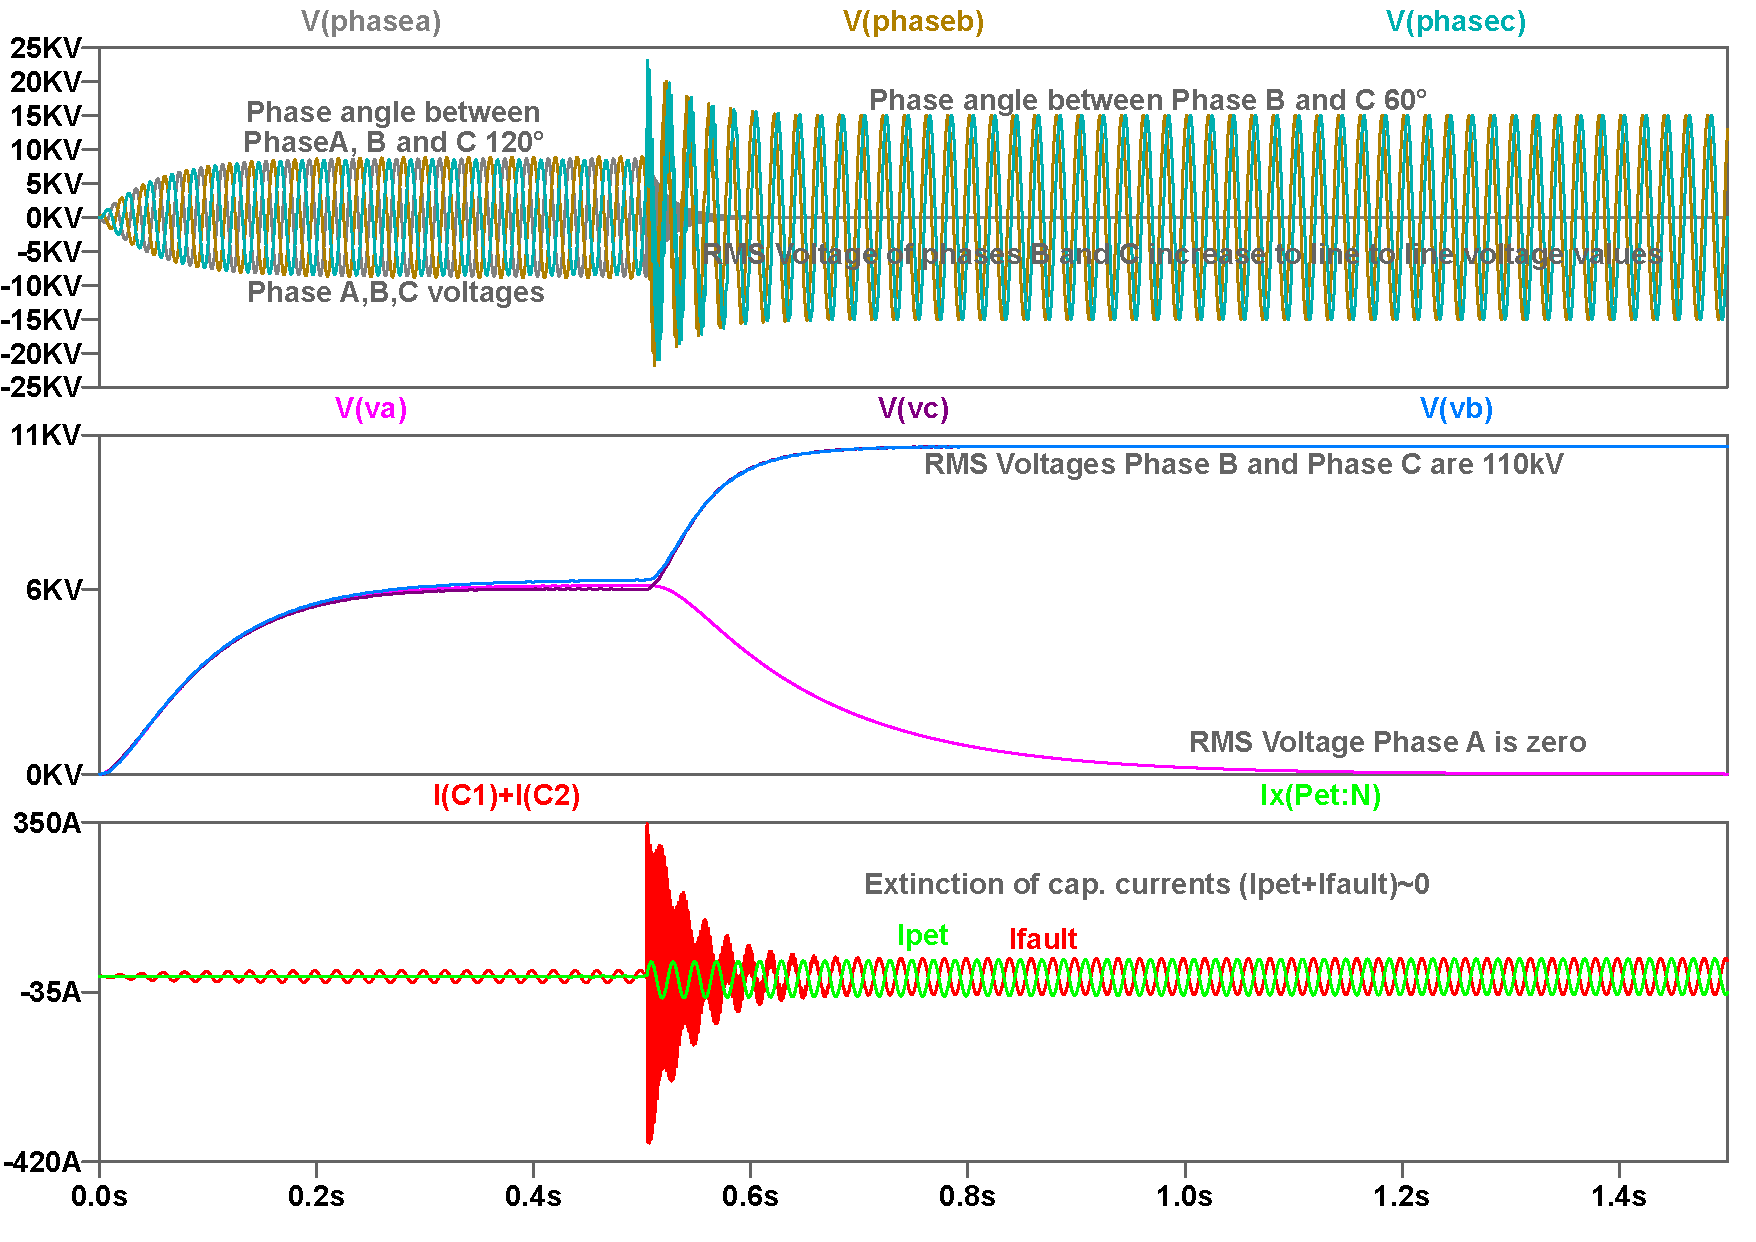
\includegraphics[width=0.90\textwidth]{figures/05_Petersen_earth_faults/Petersen_trafo_gnd_TRAN_waveform.pdf}
	\caption{Petersen without fault and external grounding transformer TRAN - waveform}
	\label{fig:Figure10}
\end{figure}

\begin{figure}[H]
	\centering
	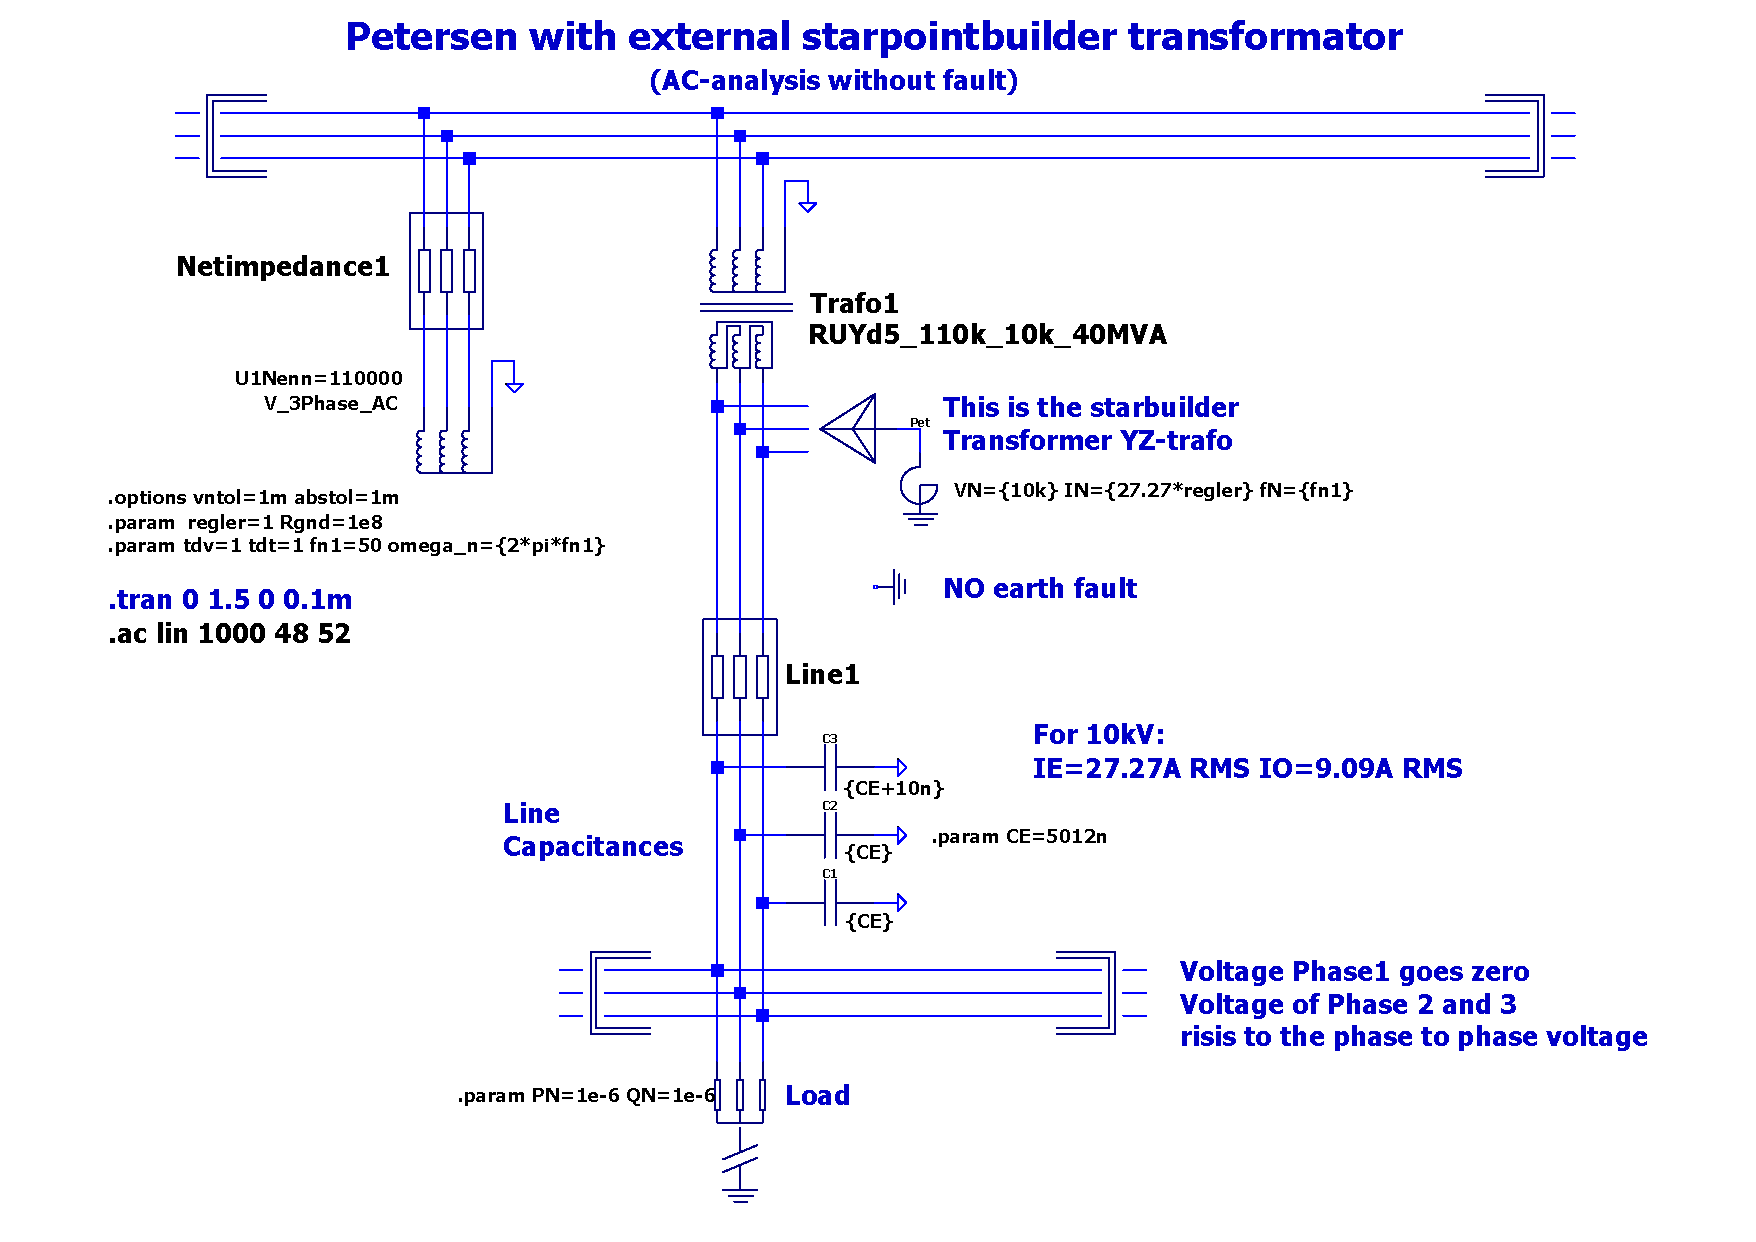
\includegraphics[width=0.90\textwidth]{figures/05_Petersen_earth_faults/Petersen_trafo_gnd_AC_no_fault_schematic.pdf}
	\caption{Petersen without fault and external grounding transformer AC - schematic}
	\label{fig:Figure11a}
\end{figure}

\begin{figure}[H]
	\centering
	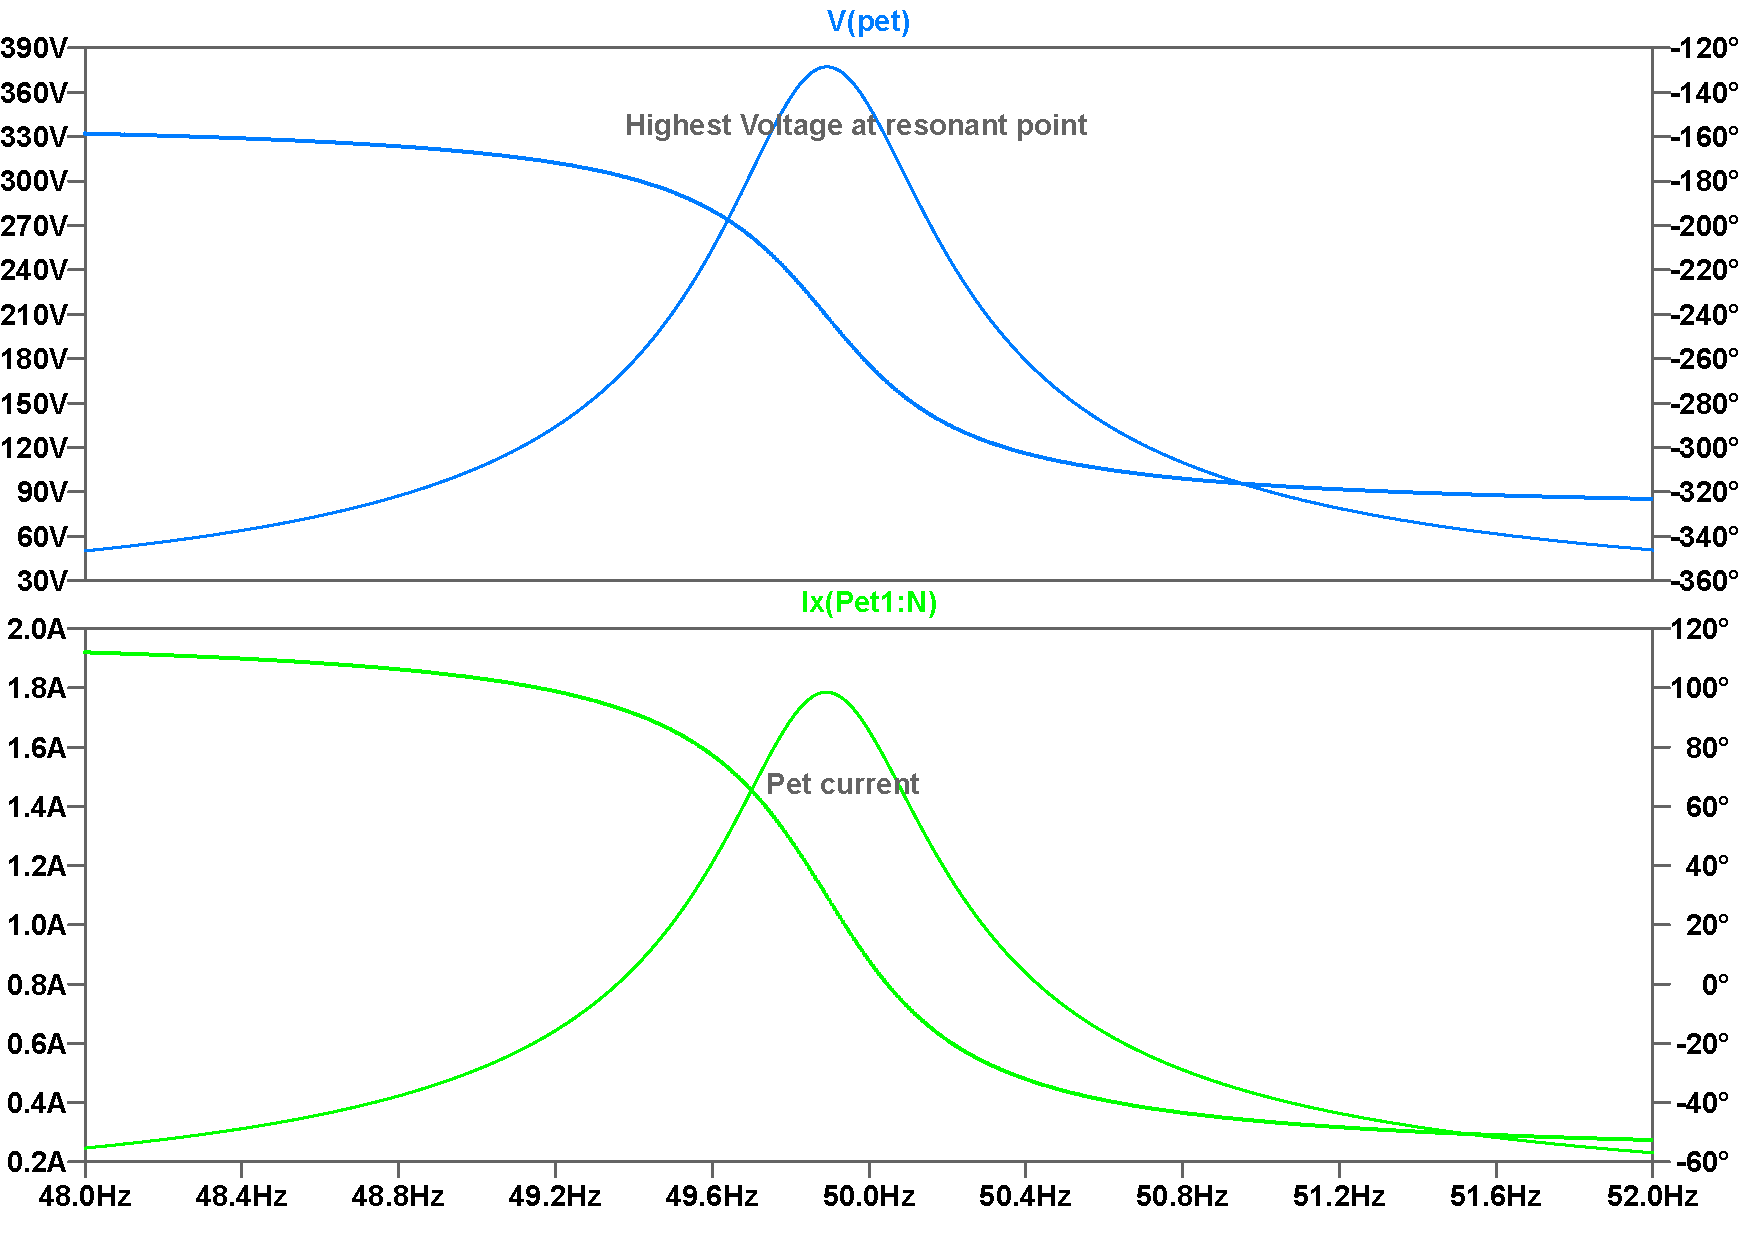
\includegraphics[width=0.90\textwidth]{figures/05_Petersen_earth_faults/Petersen_trafo_gnd_AC_no_fault_waveform.pdf}
	\caption{Petersen without fault and external grounding transformer AC - waveform}
	\label{fig:Figure11}
\end{figure}

\begin{figure}[H]
	\centering
	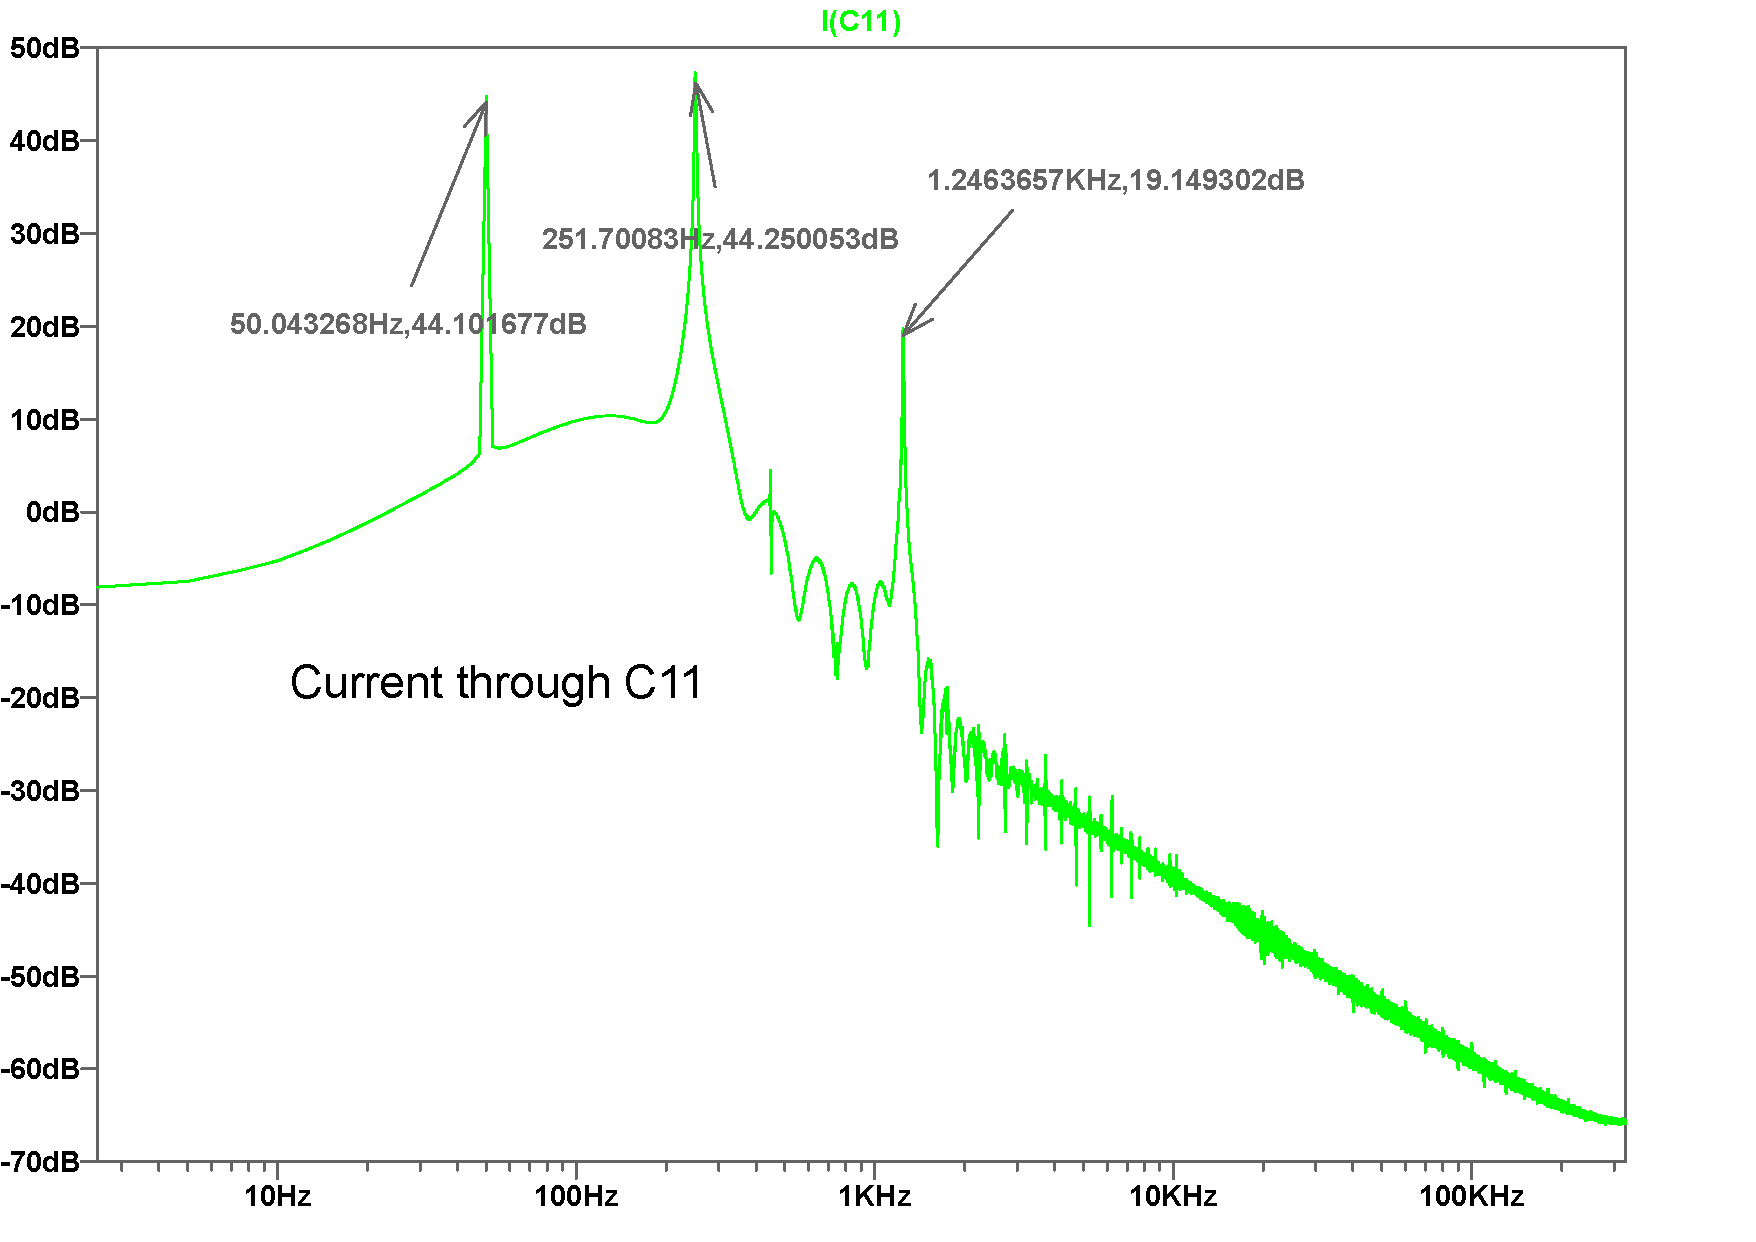
\includegraphics[width=0.70\textwidth]{figures/05_Petersen_earth_faults/Petersen_with_fault_FFT.pdf}
	\caption{FFT of current through capacitor C11}
	\label{fig:Figure13}
\end{figure}

\begin{chaptersummary}
In a resonantly earthed cable network, the Petersen coil compensates the
zero-sequence capacitive earth-fault current. Network asymmetry creates a small
neutral displacement voltage even without a fault. During a solid earth fault (currents like at a shorted circuit at startup),
the healthy phases rise toward line-to-line voltage and the capacitive reactive
power approximately doubles for the first instant. The complete tuning must include transformer and
source impedance, not only the cable capacitance. Fault inception excites
several natural frequencies determined by different inductive and capacitive
paths. For networks without an accessible neutral, a neutral-forming
transformer permits connection of the Petersen coil.
High transient currents arise during the redistribution of charge in the phase-to-earth capacitances. The capacitance of the faulted phase is discharged, while the voltages across the capacitances of the two healthy phases increase to approximately √3 times their normal values. At the higher frequencies excited by the fault, capacitive reactance decreases and inductive reactance increases. These changes contribute to the high initial currents and voltage distortion. The resonant frequencies depend on the inductances and capacitances of the relevant circuit paths.
During the earth fault, the total capacitive reactive power of the healthy phases is approximately twice the prefault three-phase value. As the transient decays, the Petersen coil compensates the additional zero-sequence earth-fault current, while the ordinary charging current remains supplied by the source.
Note: The line inductances in this particular example are modelled without mutual coupling. Including coupling can change the effective fault-path impedance and the initial peak fault current. Compare the coupled and uncoupled models discussed in Section 5.6.
\end{chaptersummary}

\chapter{Switching Whole Networks}
\label{chap:switching-whole-networks}
\index{network energization}
\index{transformer!inrush current}
\index{switching overvoltage}
\index{voltage ramp}

\section{General}
\label{sec:whole-network-general}

This chapter examines the transients that occur when an entire network (grid zone) is energized. This situation can occur during grid restoration following a blackout\\ 
The following cases are examined in detail:\\
\begin{itemize}
	\item \texttt{Connecting at minimum voltage in phase R},
	\item \texttt{Connecting the grid zone with phase R at maximum voltage},
	\item \texttt{Connecting at minimum voltage and full remanent flux},
	\item \texttt{Connecting with the main transformer set to minimum voltage},
	
	\item \texttt{Connecting a larger grid zone},
	\item \texttt{Connecting under load}.
	\item \texttt{Connecting with skin effect in the grid impedance},
	\item \texttt{Connecting with a weak feed-in},
	\item \texttt{Slowly ramping up the voltage instead of a switching operation}.
\end{itemize}

\section{Circuit Design}
Open the File \texttt{Switching\_on\_networks.asc}.
The example is a \SI{110}{\kilo\volt} network with five substations.
Three substations are loaded, two are unloaded or have loads that are not yet
connected. The network is supplied through a
\SI{220}{\kilo\volt}/\SI{110}{\kilo\volt} transformer rated
\SI{200}{\mega\volt\ampere}.

The main transformer is represented by a linear magnetizing characteristic
using the transformer parameter \texttt{m=1}. Its voltage source initially rises exponentially so that
the transformer reaches steady state before the network switch closes. The network contains three cable sections and two overhead-line sections. The cables have a total sum length of \SI{10}{\kilo\metre} and generate approximately
\SI{15}{\mega\varunit} of capacitive reactive power (see calculation \ref{calc:whole-network-petersen}). A \SI{40}{\mega\varunit} shunt reactor in bus4 overcompensates the \SI{15}{\mega\varunit} capacitive contribution, leaving a net inductive demand of approximately \SI{25}{\mega\varunit}. 
The energized network therefore tends to reduce rather than raise the voltage (under steady state conditions).

The cable phase-to-earth capacitances are compensated by a Petersen coil at
substation 1. A small capacitance asymmetry is required to create a measurable
neutral displacement voltage. In the model, this is introduced with the
parameter \texttt{cuf} in phase A of line 2.


\section{Petersen-Coil Setting}
\label{sec:whole-network-petersen-setting}

The cable capacitance is \SI{400}{\nano\farad\per\kilo\metre} per phase (see line.lib). For a
total cable length of \SI{10}{\kilo\metre}, the phase capacitance is
\SI{4000}{\nano\farad}.

\begin{calculation}{Compensation current for the complete cable network}{whole-network-petersen}
At \SI{50}{\hertz},
\begin{align}
C&=\SI{400}{\nano\farad\per\kilo\metre}\cdot\SI{10}{\kilo\metre}
  =\SI{4000}{\nano\farad},\\
X_C&=\frac{1}{\omega C}
  =\frac{1}{2\pi\cdot\SI{50}{\hertz}\cdot\SI{4000}{\nano\farad}}
  \approx\SI{796}{\ohm},\\
Q_C&=\frac{U_{\mathrm{LL}}^2}{X_C}
  =\frac{(\SI{110}{\kilo\volt})^2}{\SI{796}{\ohm}}
  \approx\SI{15.2}{\mega\varunit}.
\end{align}

For resonant earth-fault compensation,
\begin{align}
X_{L,\mathrm P}&=\frac{X_C}{3}\approx\SI{265}{\ohm},\\
I_{\mathrm P}&=\frac{U_{\mathrm{LL}}/\sqrt{3}}{X_{L,\mathrm P}}
  \approx\boxed{\SI{239.7}{\ampere}}.
\end{align}
\end{calculation}

The Petersen model uses a rounded setting of \SI{250}{\ampere}. An increase of roughly
\SI{5}{\percent} is useful because internal transformer reactance reduces the
neutral voltage and prevents the ideal coil current from being reached during
an earth fault. This effect was discussed in detail in
\cref{chap:earth-faults}.

\section{Calculation of the Network Resonance}
\label{sec:whole-network-resonance}

The inductances specified on the \SI{220}{\kilo\volt} side must be referred to
the \SI{110}{\kilo\volt} side. With a voltage ratio of 2, impedance and
inductance are divided by $2^2=4$ when referred from the
\SI{220}{\kilo\volt} side to the \SI{110}{\kilo\volt} side. 
The source and transformer inductances are $L_{\mathrm{net}}=\SI{0.0077}{\henry}$ and $L_{\mathrm{Tr}}=\SI{0.154}{\henry}$. The transformer value is obtained from
\texttt{xkos/omega} in \texttt{Trafo\_YY0\_220k\_110k\_200MVA\_Daten.asc}. Thus, ..



\begin{calculation}{Dominant cable-network resonance}{whole-network-resonance}
	\begin{align}
		L_{\mathrm{eq}}&=\frac{L_{\mathrm{net}}}{4}
		+\frac{L_{\mathrm{Tr}}}{4}
		=\frac{\SI{0.0077}{\henry}+\SI{0.154}{\henry}}{4}
		=\SI{0.04}{\henry},\\
		C&=\SI{4000}{\nano\farad},\\
		f_{\mathrm r}&=\frac{1}{2\pi\sqrt{L_{\mathrm{eq}}C}}
		\approx\boxed{\SI{395.8}{\hertz}}.
	\end{align}
\end{calculation}

This result agrees with the approximately \SI{400}{\hertz} peak, which is most clearly visible (after simulation) in
the FFT of the main transformer current in phases B and C in Case 1. Zoom into the interval from 40 ms to 100 ms, then select View → FFT and use the current zoom extent.
Additional harmonics caused by the nonlinear transformer currents are most clearly visible in phase A at 100 Hz, 150 Hz, 200 Hz and 250 Hz.

\section{Rated current of the main transformer}
\label{sec:whole-network-case1-values}

The rated RMS current on the \SI{220}{\kilo\volt} side of the main transformer
is

\begin{equation}
	I_N=\frac{S_N}{\sqrt{3}U_N}
	=\frac{\SI{200}{\mega\volt\ampere}}
	{\sqrt{3}\cdot\SI{220}{\kilo\volt}}
	\approx\boxed{\SI{525}{\ampere}}.
\end{equation}

\noindent For further values of transformer parameters see: \\
Transformer\_110kV\_10KV.asc for the medium voltage transformer and \\
Transformer\_220kV\_110KV.asc for the high voltage transformere


\section{Case 1: Closing at the Phase-R Voltage Zero} 
\label{sec:network-closing-voltage-zero}

NOTE: The ltspice file for all cases except case9 is \texttt{Switching\_on\_networks.asc}.
To view the results in the Waveform Viewer, you must select the appropriate plot file. After the simulation, open the Waveform Viewer window. Select “Plot Settings” / “Open Plot Settings File” and, from the available plots, select one of the corresponding case1 plots. Plots of voltages, currents, and magnetic fluxes are available.
For the different simulations some parameters in the schematic are changed. 
With \texttt{t0=0} the network switch closes at \SI{40}{\milli\second}, when
the phase A voltage crosses zero. The primary phase A current of the main
transformer is then dominated by the magnetizing inrush currents of the
medium-voltage transformers. Closing at voltage zero produces the largest
unidirectional flux offset in Phase A (U). Even without residual flux, the transient flux can
approach twice its steady-state peak starting from zero to about \SI{0.58}{\weber}.

At the same instant, the phase A (U) capacitive charging current is comparatively
small because the applied voltage is close to zero. In phases B (V) and C (W), the
opposite situation occurs: the instantaneous voltages are high, their medium-voltage
transformer flux offsets are smaller, and their initial cable-charging currents
are large. The principal currents decay over approximately
\SI{500}{\milli\second}. The over-voltages depends strongly on the switching instant. 


All three phase currents contain high-frequency components caused by resonances
between the cable capacitances and the source and transformer inductances. An
FFT of a phase A medium-voltage-transformer current also contains many
harmonics (100Hz,150Hz,200Hz,250Hz) of the power frequency because of the nonlinear transformer
magnetizing curves. In phases B and C, a distinct network resonance appears at
approximately \SI{400}{\hertz}.\\

All three medium voltage transformer currents exhibit similar but also slightly different behaviour. Since a Petersen coil is connected to the neutral point of Transformer 1, the inrush-current waveform partly extends below zero. For Transformer 2, a faster decay of the inrush current can be observed. This can be explained by the additional voltage drop caused by the shunt reactor current on Line 2. In Phase A, the shunt reactor carries a current that remains entirely positive (in phase with the transformer). This current causes a greater voltage drop across Line 2 and thus a lower voltage across the transformer. Since the flux of the transformer depends directly on the integral of the voltage, both the flux and the current of the transformer decrease. NOTE: The behaviour described above occurs only if the shunt reactor is turned on simultaneously with the transformer. If the shunt reactor is turned on 10 ms later, its current is out of phase with the transformer current, and the inrush current of the transformer will now decrease more slowly or even rise slightly at first. Try it out by inserting a switch with a switching time of 50 ms before the shunt reactor.

Lines 3 and 4 are overhead lines, so their capacitive charging transients are much lower than those of the cables.
For Schematic and waveforms see figures \ref{fig:figure61}-\ref{fig:figure66}. 
For measured values and signal ranges, see Table \ref{tab:measurement-values-case1}.\\



%\begin{figure}[H]
%	\centering
%	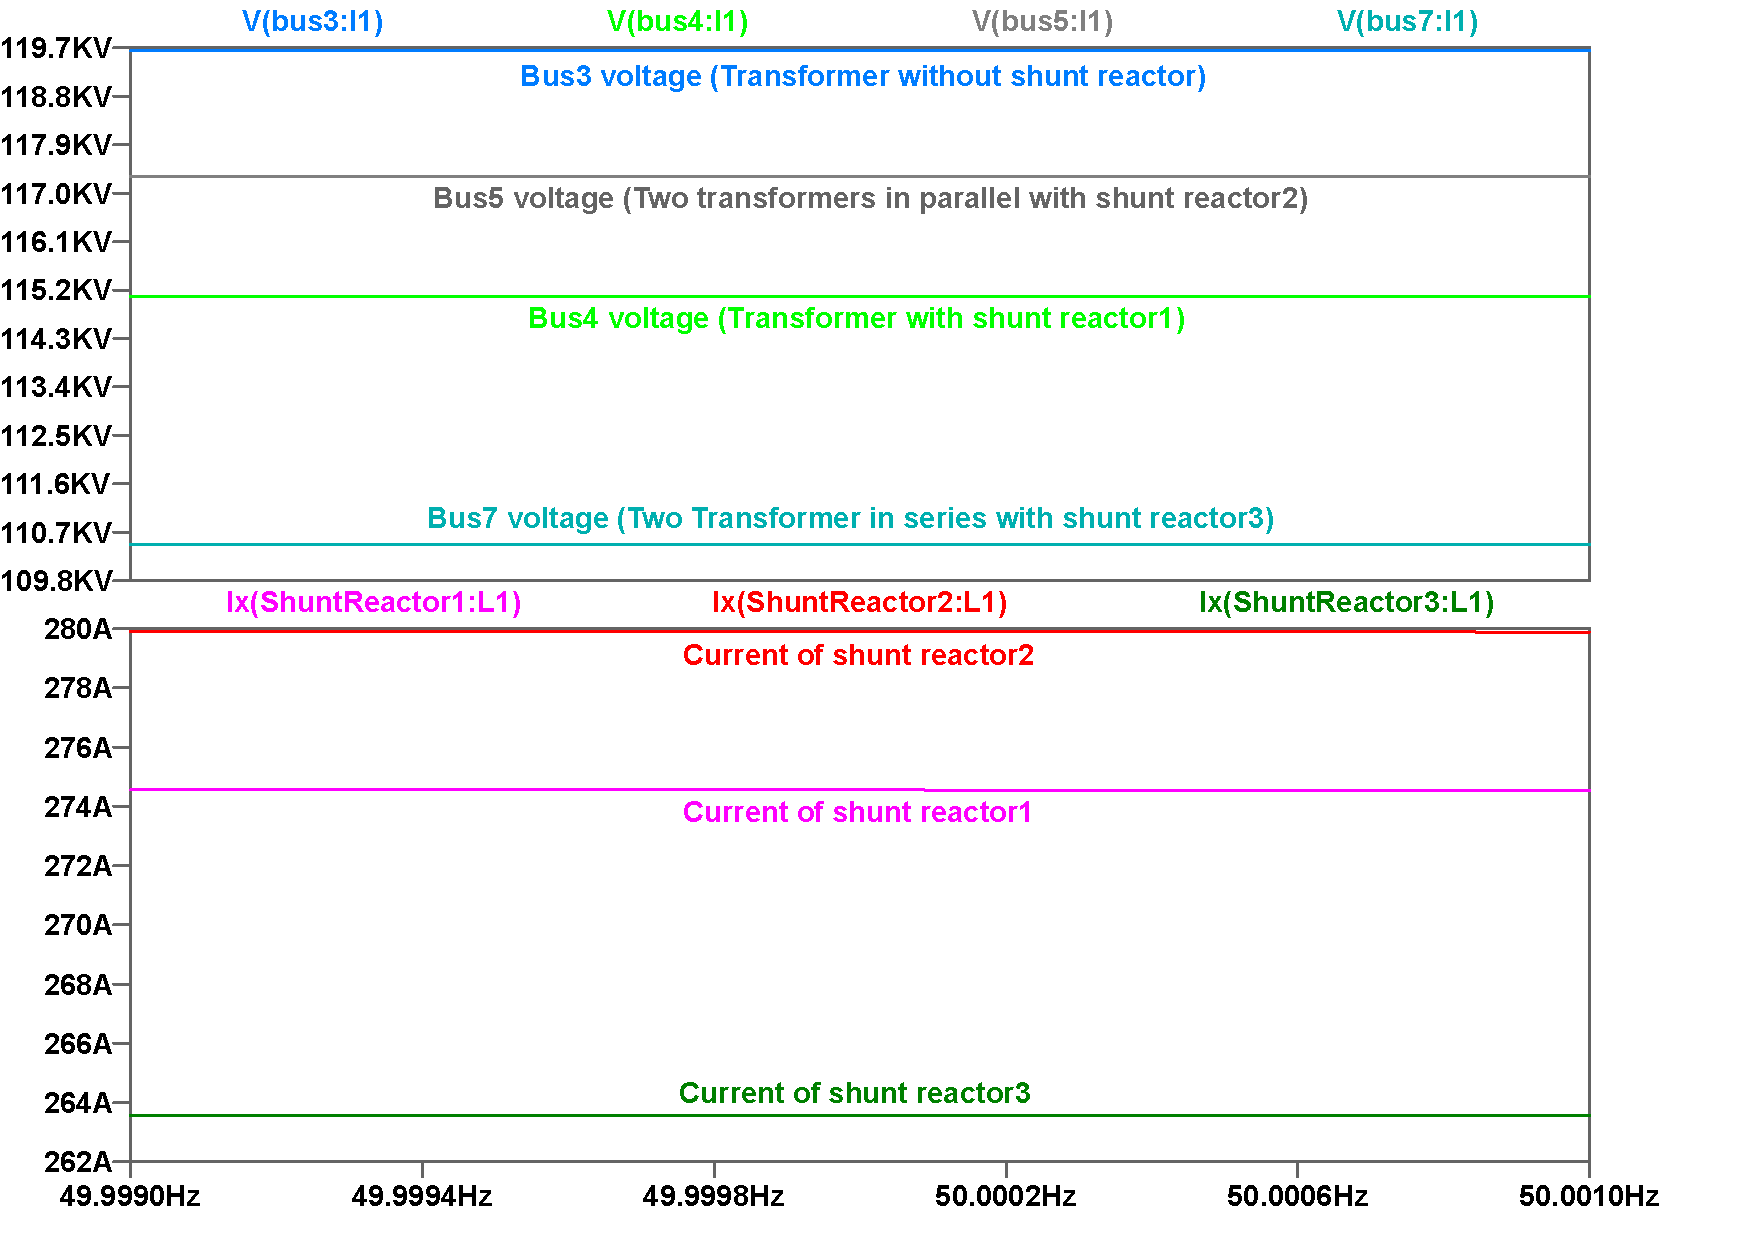
\includegraphics[width=0.90\textwidth]{figures/01_Transformer und shunt reactor/Transformer_and_shunt_reactor_AC_waveform}
%	\caption{AC voltages and currents at the shunt reactors}
%	\label{fig:Transformer_and_shunt_reactor_AC_Waveform}
%\end{figure}

\begin{figure}[H]
	\centering
	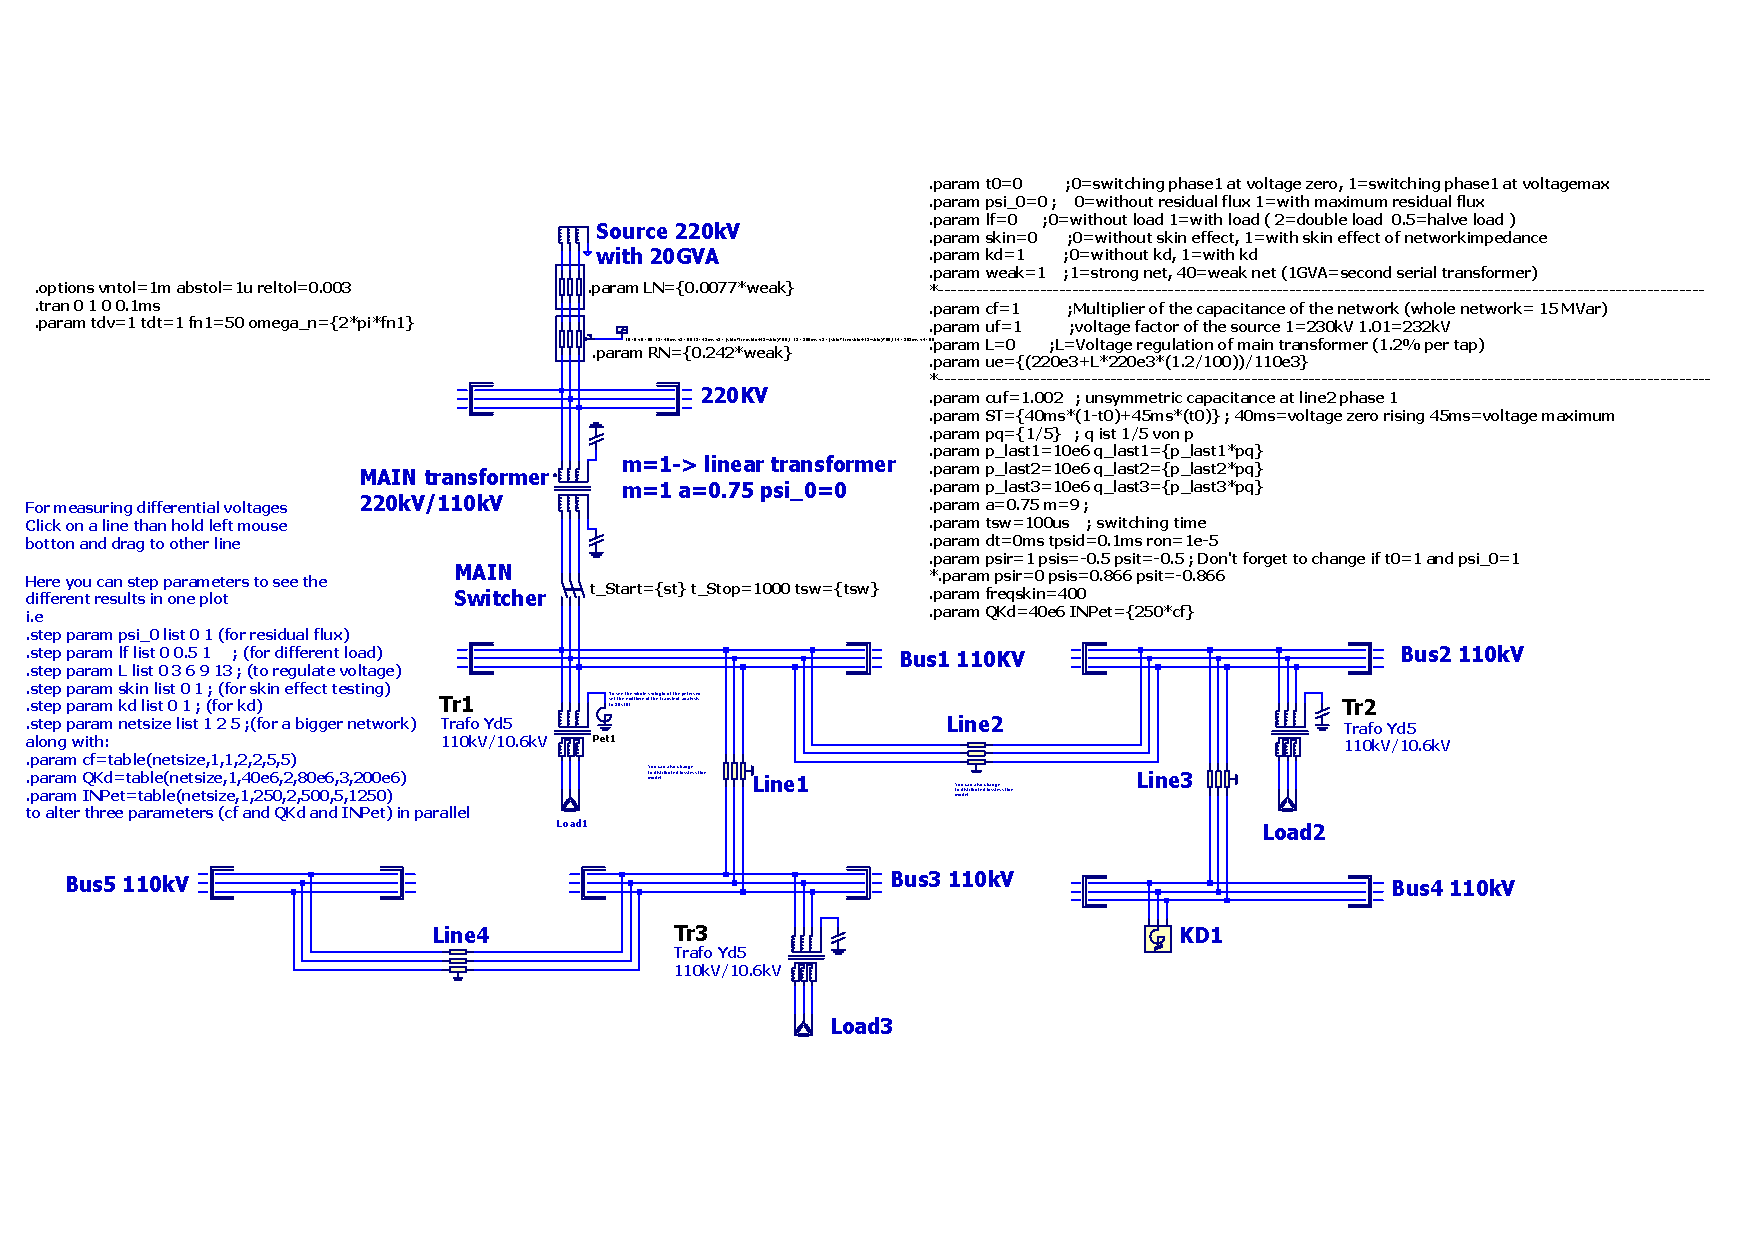
\includegraphics[width=0.9\textwidth]{figures/06_Switching_on_networks/Switching_on_networks_schematic}
	\caption{Switching on networks schematic - case1}
	\label{fig:figure61}
\end{figure}

\begin{figure}[H]
	\centering
	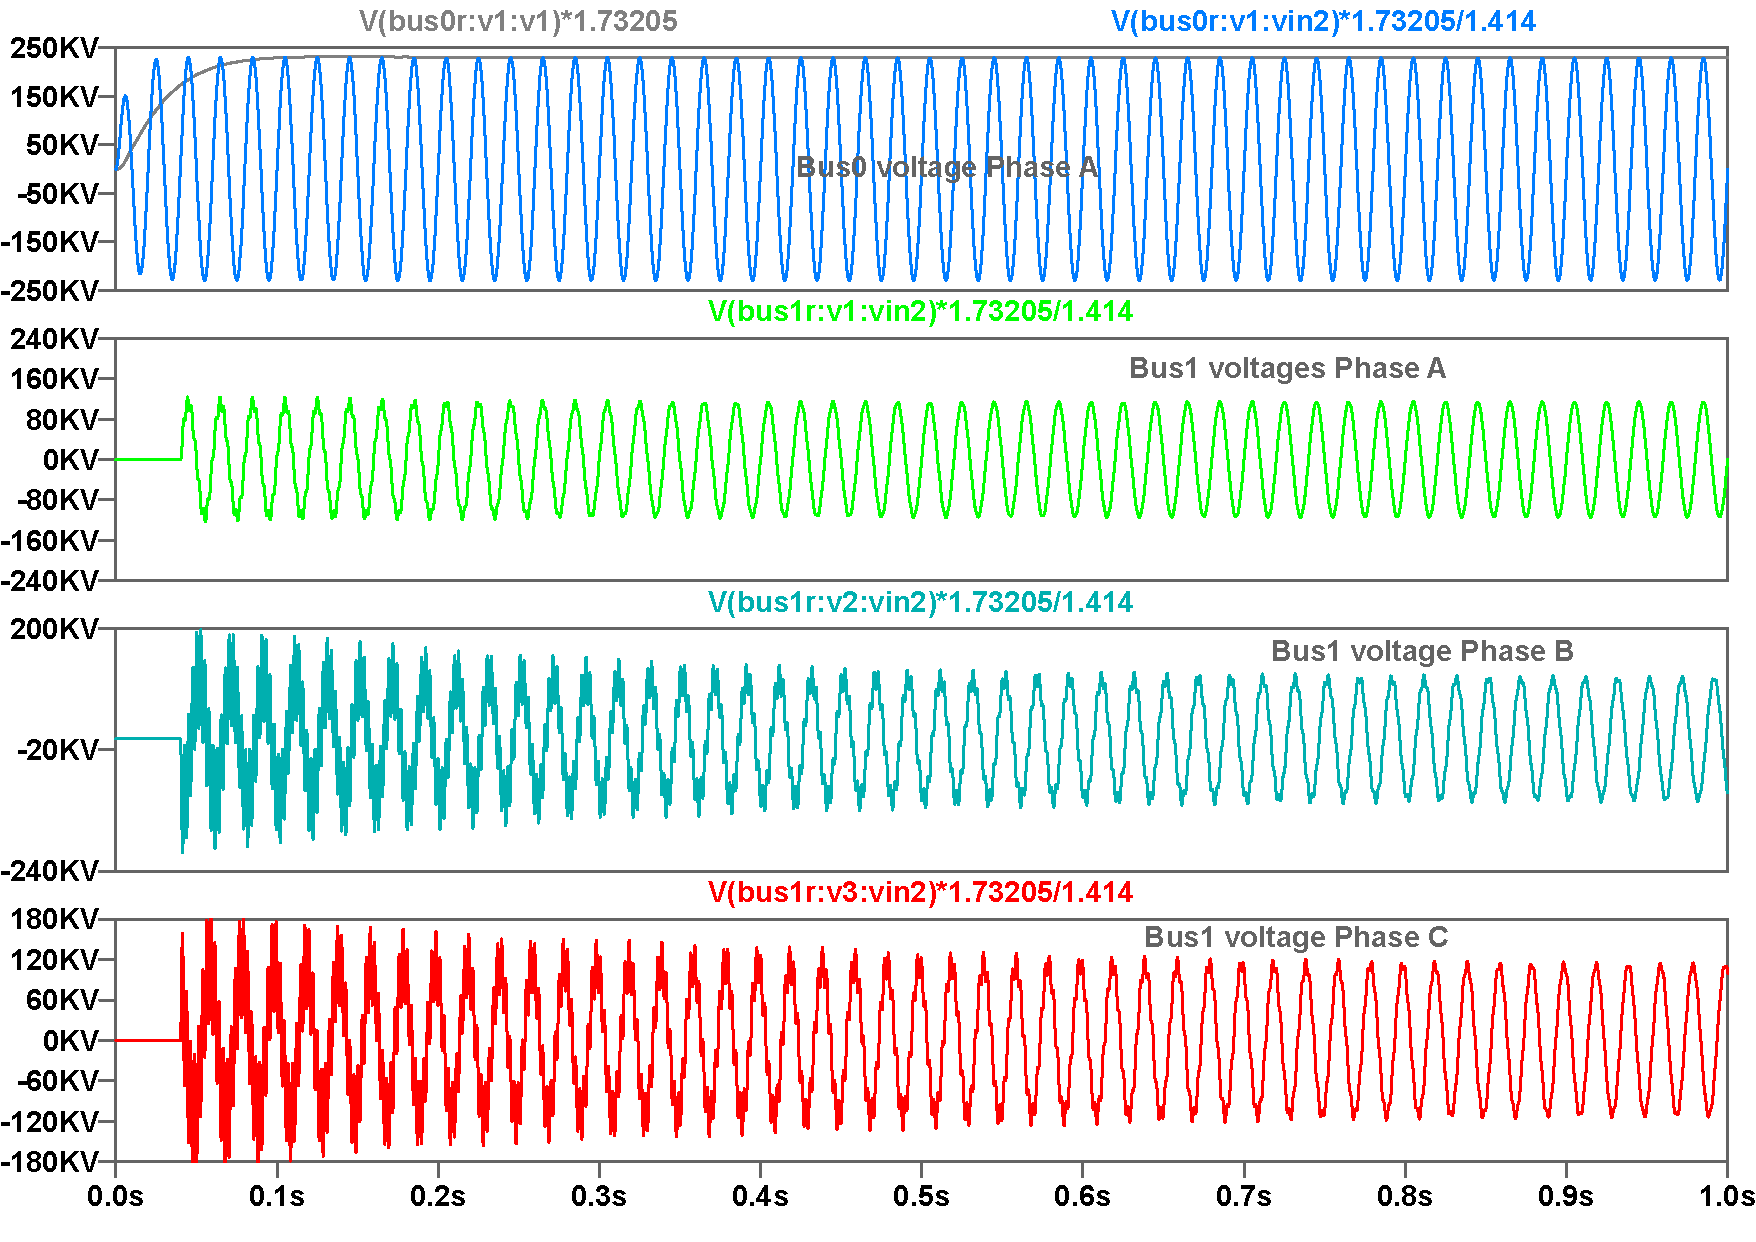
\includegraphics[width=0.90\textwidth]{figures/06_Switching_on_networks/Switching_on_networks_Bus0_Bus1_voltages-case1}
	\caption{Switching on networks voltages - case1}
	\label{fig:figure62}
\end{figure}

\begin{figure}[H]
	\centering
	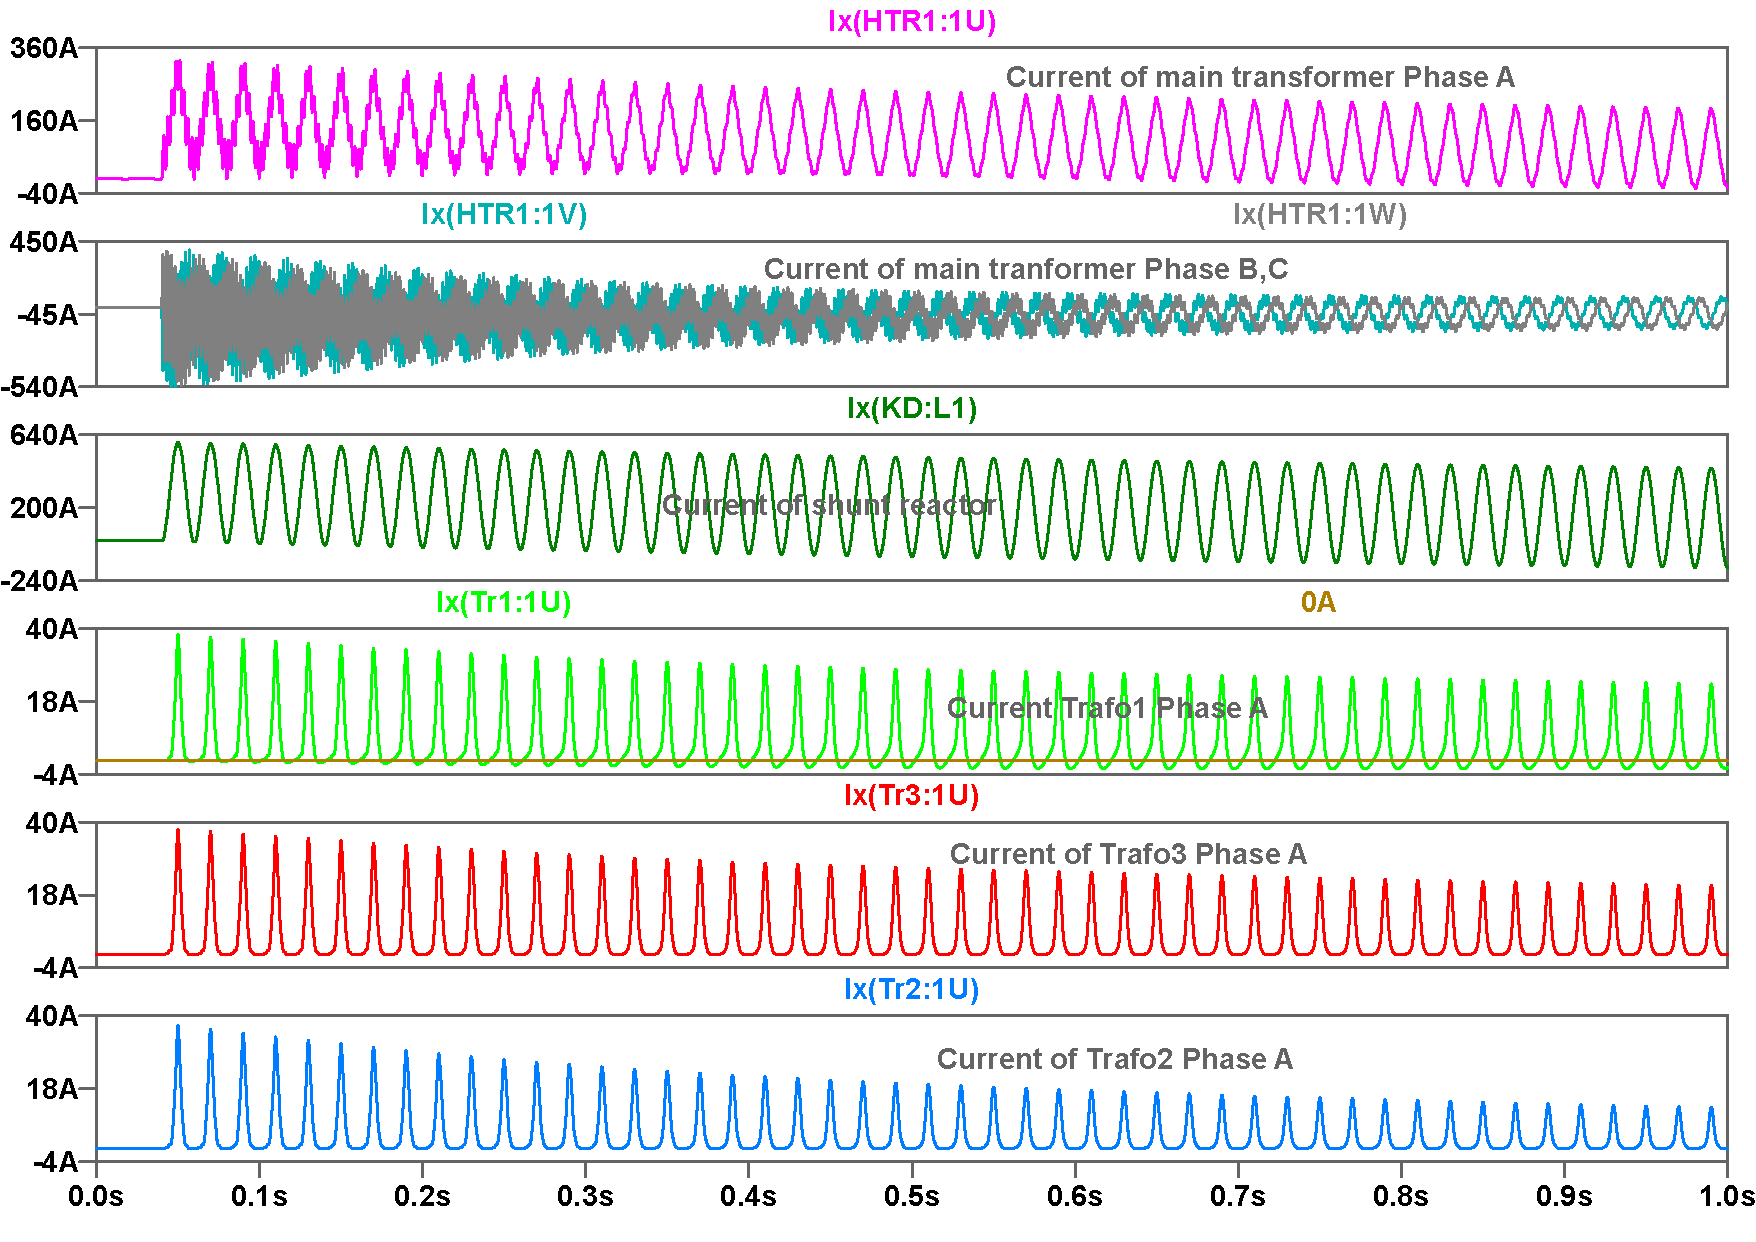
\includegraphics[width=0.90\textwidth]{figures/06_Switching_on_networks/Switching_on_networks_currents-case1}
	\caption{Switching on networks currents - case1}
	\label{fig:figure63}
\end{figure}

\begin{figure}[H]
	\centering
	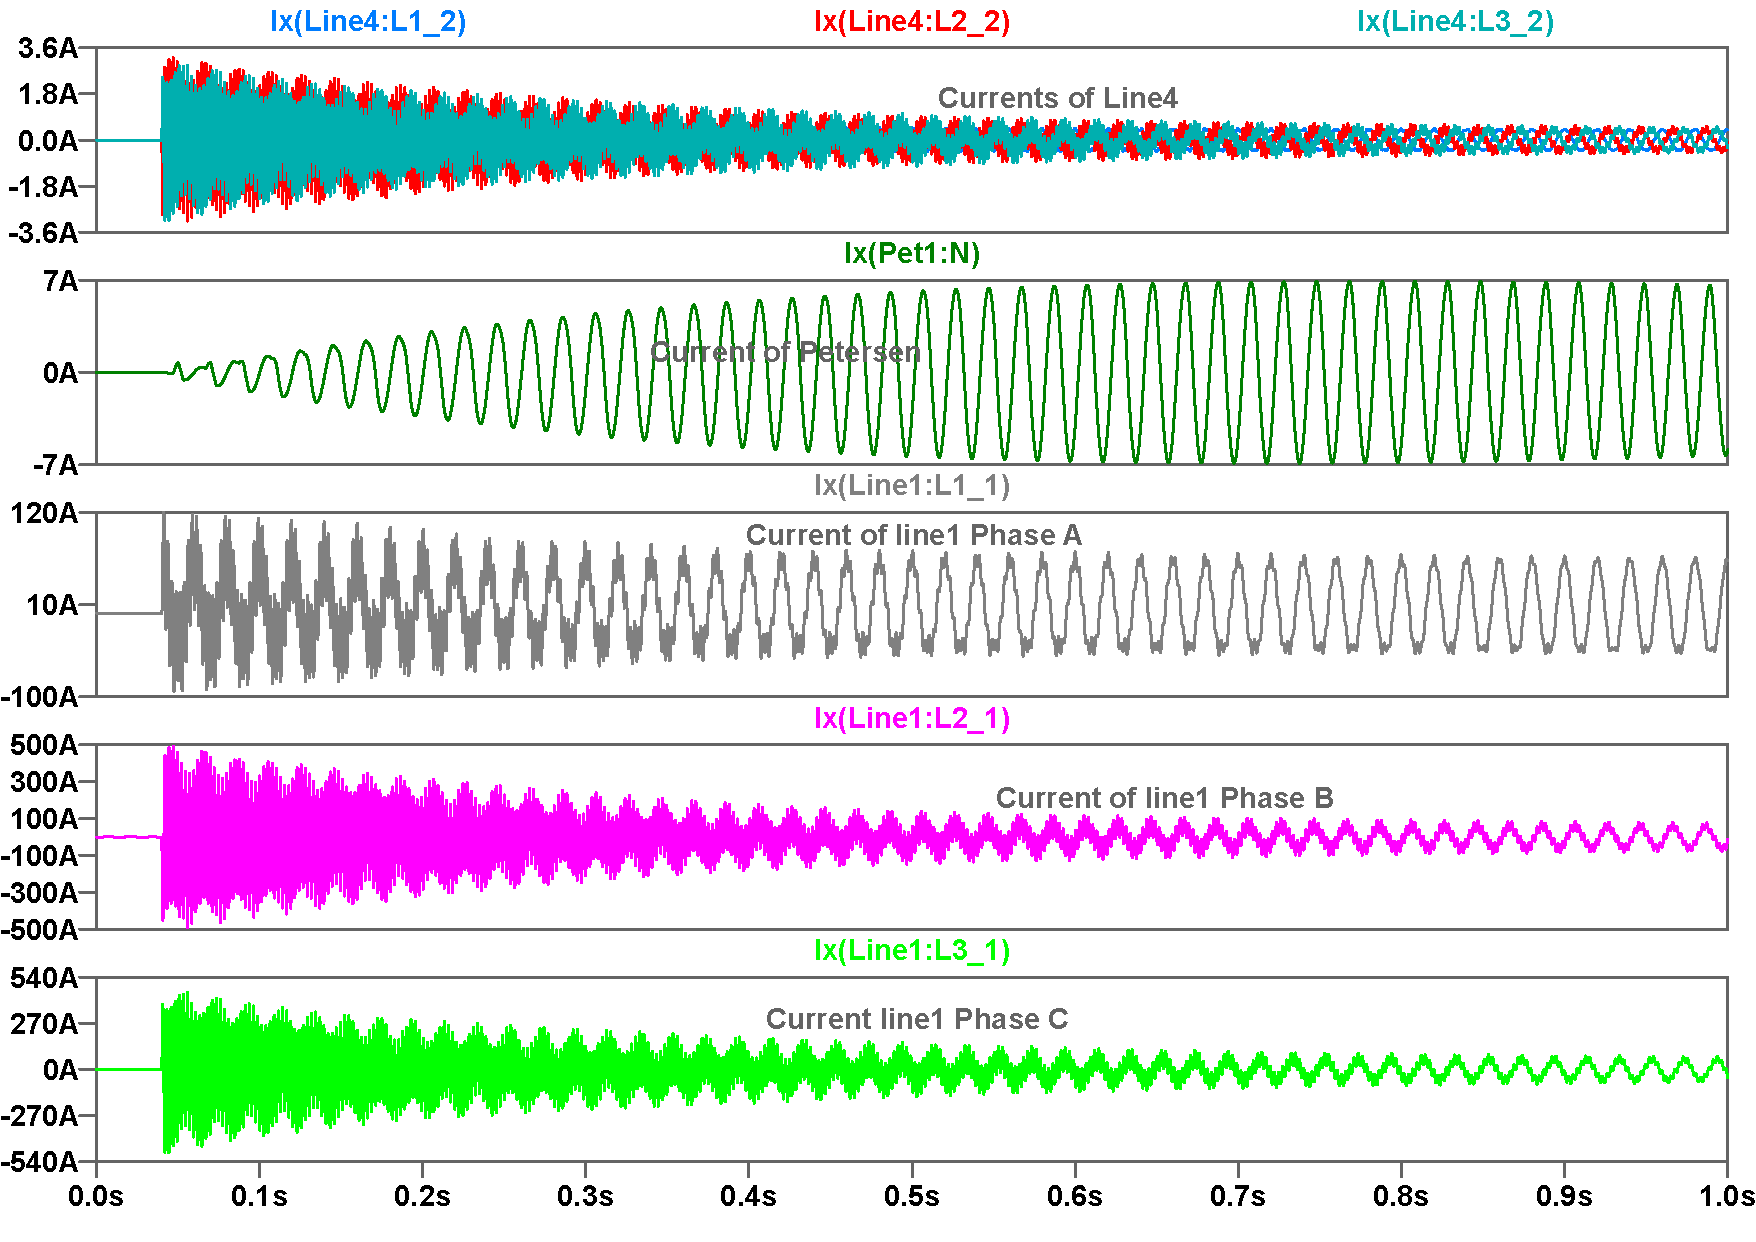
\includegraphics[width=0.90\textwidth]{figures/06_Switching_on_networks/Switching_on_networks_currents_Line1_Line4-case1}
	\caption{Switching on networks currents line1, line4 - case1}
	\label{fig:figure64}
\end{figure}

\begin{figure}[H]
	\centering
	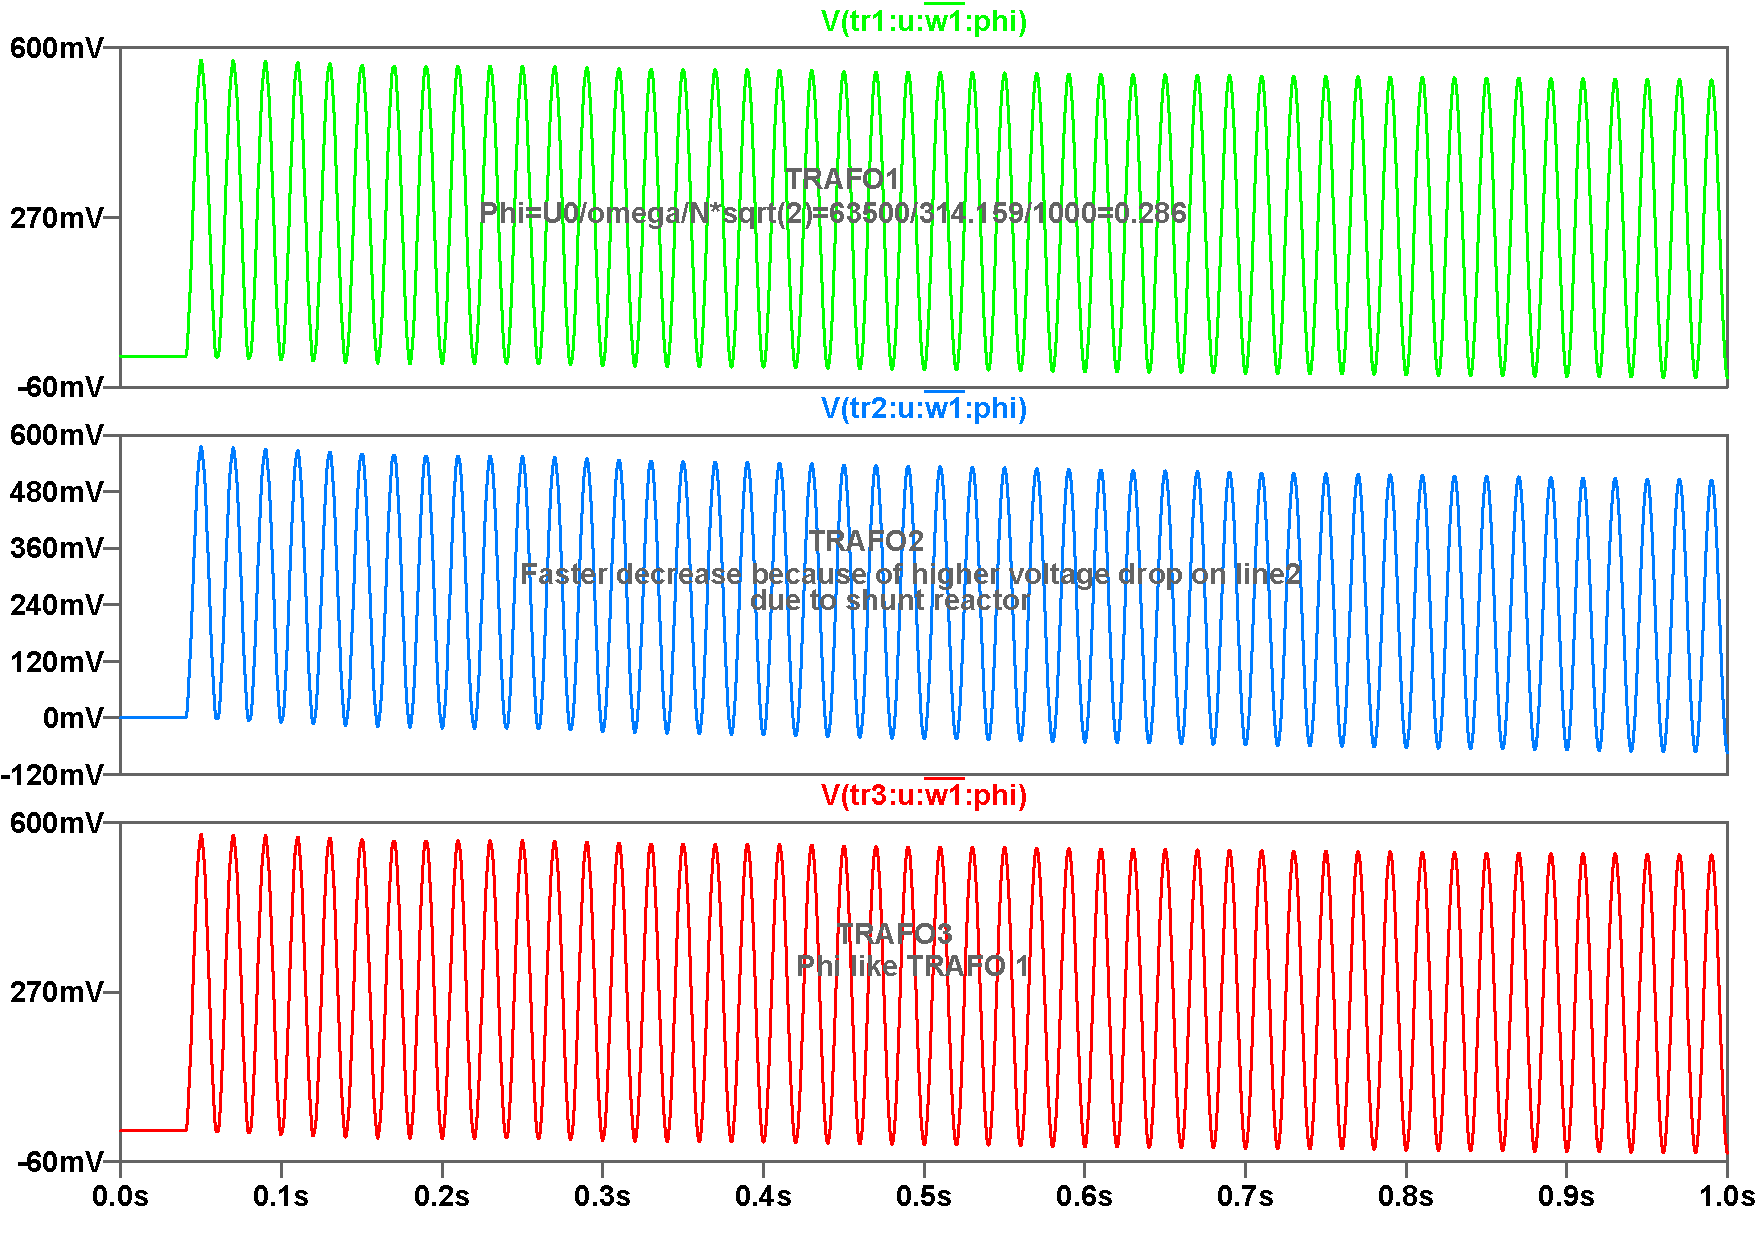
\includegraphics[width=0.90\textwidth]{figures/06_Switching_on_networks/Switching_on_networks_phi-case1}
	\caption{Switching on networks fluxes - case1}
	\label{fig:figure65}
\end{figure}

\begin{figure}[H]
	\centering
	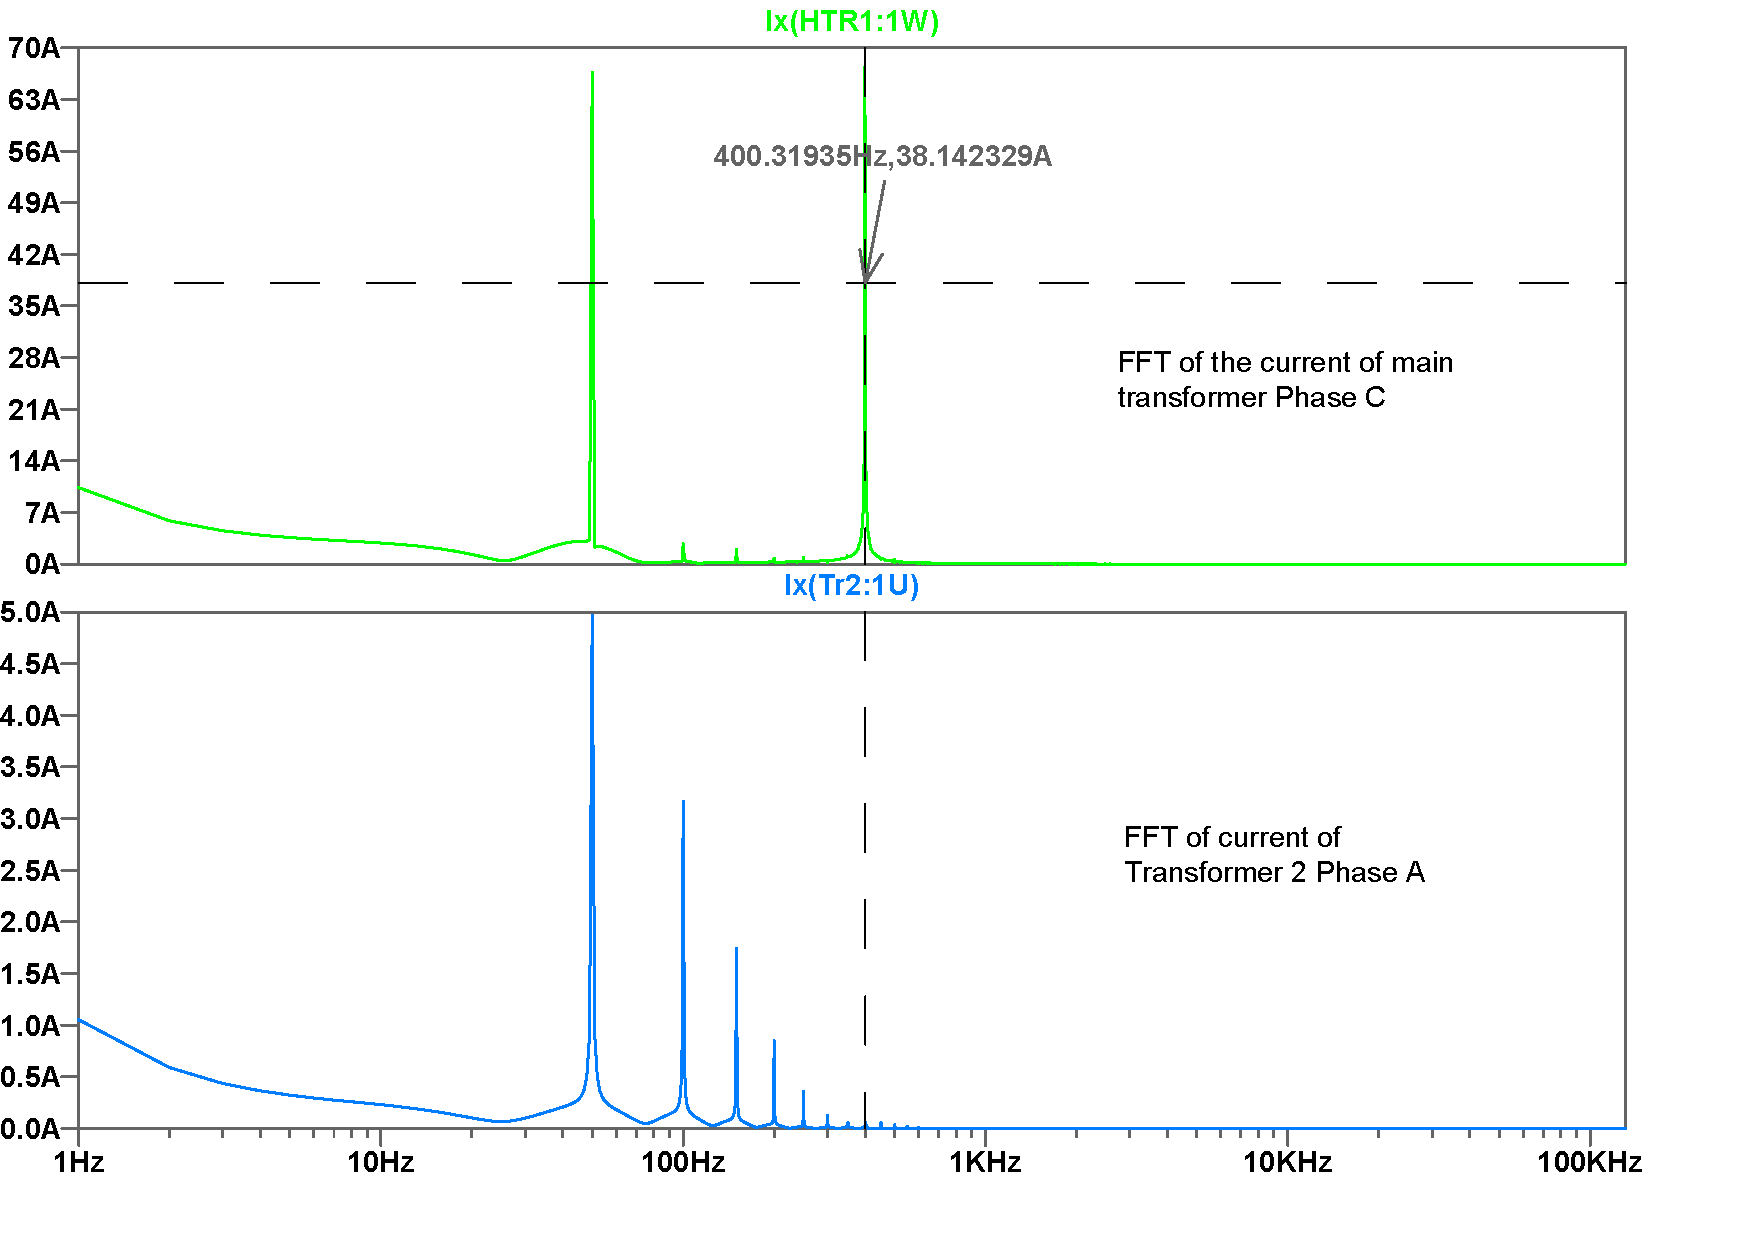
\includegraphics[width=0.90\textwidth]{figures/06_Switching_on_networks/Switching_on_networks_FFT_Transformer-case1}
	\caption{Switching on networks FFT - case1}
	\label{fig:figure66}
\end{figure}

% Measurement values table for the Power System Simulation book.
% Required packages are already loaded by the central preamble:
% booktabs, tabularx, array, siunitx, xcolor.

\begin{table}[htbp]
  \centering
  \caption{Signal ranges for Case 1. All values are peak values, bus values are multiplied by 1.73/1.414}
  \label{tab:measurement-values-case1}
  \small
  \setlength{\tabcolsep}{3.5pt}
  \renewcommand{\arraystretch}{1.18}
  \begin{tabularx}{\textwidth}{@{}
      >{\raggedright\arraybackslash}p{0.055\textwidth}
      >{\raggedright\arraybackslash}p{0.085\textwidth}
      >{\raggedright\arraybackslash}p{0.095\textwidth}
      >{\raggedright\arraybackslash}p{0.105\textwidth}
      >{\raggedright\arraybackslash}p{0.075\textwidth}
      >{\raggedright\arraybackslash}p{0.075\textwidth}
      Y@{}}
    \toprule
    \textbf{Meas.} &
    \textbf{Grid element} &
    \textbf{Phase} &
    \textbf{Voltage level} &
    \textbf{Min.} &
    \textbf{Max.} &
    \textbf{Notes} \\
    \midrule
    $V$ & Bus0  & Ph A       & \SI{220}{\kilo\volt} & \SI{-229}{\kilo\volt} & \SI{229}{\kilo\volt} & -- \\
    $V$ & Bus1  & Ph A & \SI{110}{\kilo\volt} & \SI{-100}{\kilo\volt} & \SI{100}{\kilo\volt} & -- \\
     $V$ & Bus1  & Ph B, C & \SI{110}{\kilo\volt} & \SI{-200}{\kilo\volt} & \SI{200}{\kilo\volt} & -- \\
    $I$ & HTr1  & Ph A       & \SI{220}{\kilo\volt} & \SI{0}{\ampere} & \SI{330}{\ampere} & -- \\
    $I$ & HTr1  & Ph B, C    & \SI{220}{\kilo\volt} & \SI{-540}{\ampere} & \SI{360}{\ampere} & -- \\
    $I$ & KD1   & Ph A       & \SI{110}{\kilo\volt} & \SI{0}{\ampere} & \SI{600}{\ampere} & Steady state: \SI{300}{\ampere} \\
    $I$ & Tr1   & Ph A       & \SI{110}{\kilo\volt} & \SI{-2}{\ampere} & \SI{38}{\ampere} & Due to Petersen values under zero line \\
    $I$ & Tr2   & Ph A       & \SI{110}{\kilo\volt} & \SI{0}{\ampere} & \SI{37}{\ampere} & Due to KD1: faster decrease of current \\
    $I$ & Tr3   & Ph A       & \SI{110}{\kilo\volt} & \SI{0}{\ampere} & \SI{37}{\ampere} & -- \\
    $I$ & Line4 & Ph B, C & \SI{110}{\kilo\volt} & \SI{-3}{\ampere} & \SI{3}{\ampere} & Small capacitive inrush current due to overhead line \\
    $I$ & Line1 & Ph B, C & \SI{110}{\kilo\volt} & \SI{-500}{\ampere} & \SI{500}{\ampere} & High capacitive inrush current due to cable \\
     $I$ & Line1 & Ph A  & \SI{110}{\kilo\volt} & \SI{-100}{\ampere} & \SI{120}{\ampere} & -- \\
     $I$ & Pet1 & Ph N & \SI{110}{\kilo\volt} & \SI{-7}{\ampere} & \SI{7}{\ampere} & Longtime value very small \\
    $V$ & Pet1 & Ph N & \SI{110}{\kilo\volt} & \SI{-1.8}{\kilo\volt} & \SI{1.6}{\kilo\volt} & Longtime value very small \\
    $\Phi$ & Tr1 & Ph A      & \SI{110}{\kilo\volt} & \SI{0}{\weber} & \SI{0.576}{\weber} & Nominal flux: \SI{0.288}{\weber} \\
    FFT & HTr1  & Ph C       & \SI{220}{\kilo\volt} & \SI{50}{\hertz} & \SI{400}{\hertz} & Only \SI{50}{\hertz} and \SI{400}{\hertz} \\
    FFT & Tr2   & Ph A       & \SI{110}{\kilo\volt} & \SI{50}{\hertz} & \SI{250}{\hertz} & \SI{50}{\hertz}, \SI{100}{\hertz}, \SI{150}{\hertz}, \SI{200}{\hertz}, and \SI{250}{\hertz} \\
    \bottomrule
  \end{tabularx}
\end{table}


%\include{chapters/06_Switching Whole Networks/measurement_values.tex}


\section{Case 2: Closing at the Phase-R Voltage Maximum} 
\label{sec:network-closing-voltage-maximum}

Set \texttt{t0=1}. Phase A now closes near its voltage maximum. Its initial
capacitive charging current measured at the primary side of the main transformer is at its maximum, while the magnetising inrush currents of transformers 1, 2 and 3 - because of the corresponding flux - begins close to its natural
steady-state trajectory. Phases B and C contain mixtures of cable-charging and
transformer-magnetizing currents.
The currents of the main transformer 
decay toward steady state within approximately \SI{500}{\milli\second}. The
largest voltage peak occurs in phase A, while phases B and C show similar,
smaller peaks.

The primary currents of the main transformer remain approximately at the level of Case 1. The inrush currents of medium-voltage transformers 1, 2, and 3 are now minimal in Phase A and higher and roughly equal in Phases B and C for transformers 2 and 3, but remain smaller than the inrush currents in Phase A at the switching time t0 = 0. Since the Petsersen current of Transformer 1 becomes quite high at approximately 16 A when t0 = 1, the currents in phases B and C of Transformer 1 differ. The current through the shunt reactor is now symmetrical about zero from the start and is approximately 300 A. The current in Line 1 Phase A is approximately 500 A, and that in Phases B and C is approximately 300 A. The magnetic flux in phases B and C is now at its highest, but not as high as it was in Phase A in Case 1. Therefore the inrush currents of Phase B and C are smaller than those in phase A of Case 1.
NOTE: Due to the highly nonlinear magnetic characteristic curve, small changes in the flux values cause large changes in the magnetization currents.  
For Waveforms see figures \ref{fig:figure67}-\ref{fig:figure610}. 
For Measurement values and signal ranges see table: \ref{tab:measurement-values-case2}.\\

\begin{figure}[H]
	\centering
	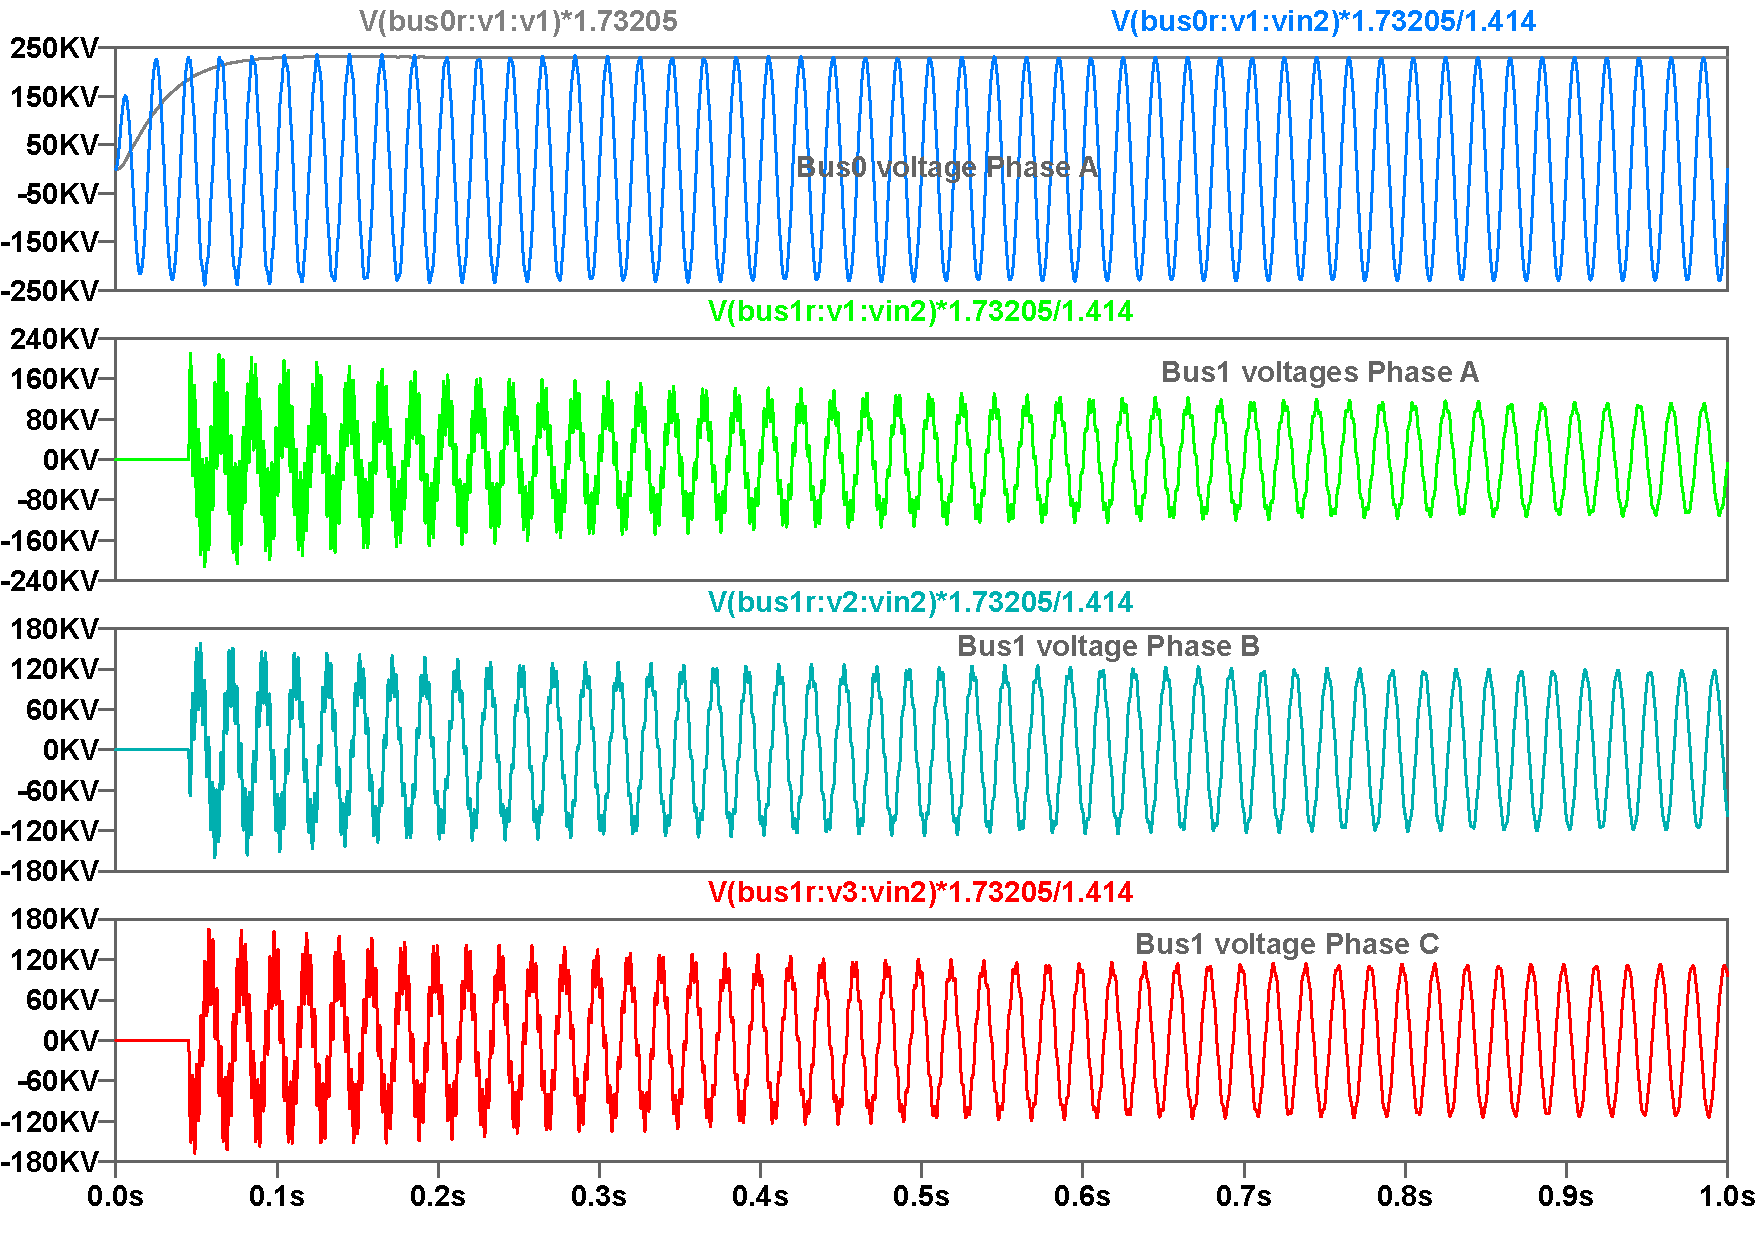
\includegraphics[width=0.90\textwidth]{figures/06_Switching_on_networks/Switching_on_networks_Bus0_Bus1_voltages-case2}
	\caption{Switching on networks voltages - case2}
	\label{fig:figure67}
\end{figure}

\begin{figure}[H]
	\centering
	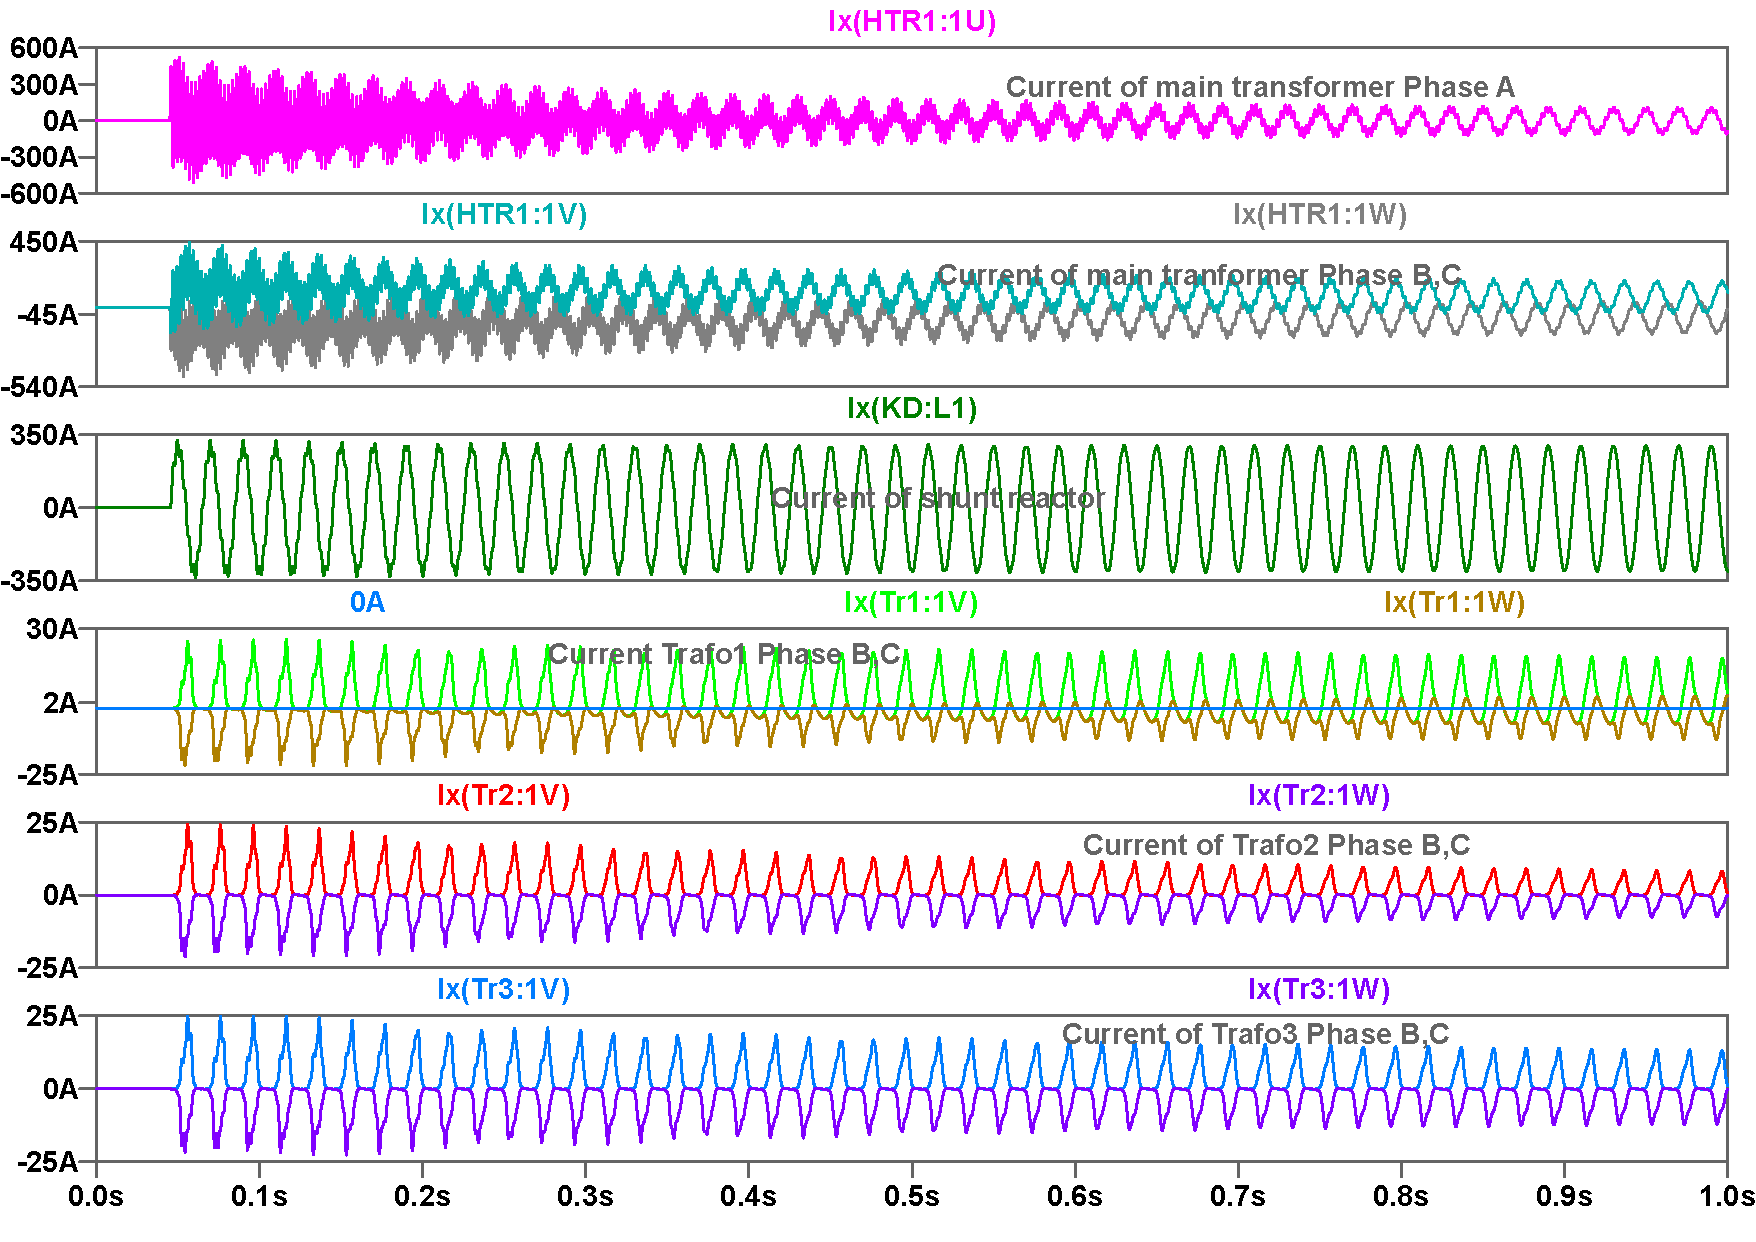
\includegraphics[width=0.90\textwidth]{figures/06_Switching_on_networks/Switching_on_networks_currents-case2}
	\caption{Switching on networks currents - case2}
	\label{fig:figure68}
\end{figure}

\begin{figure}[H]
	\centering
	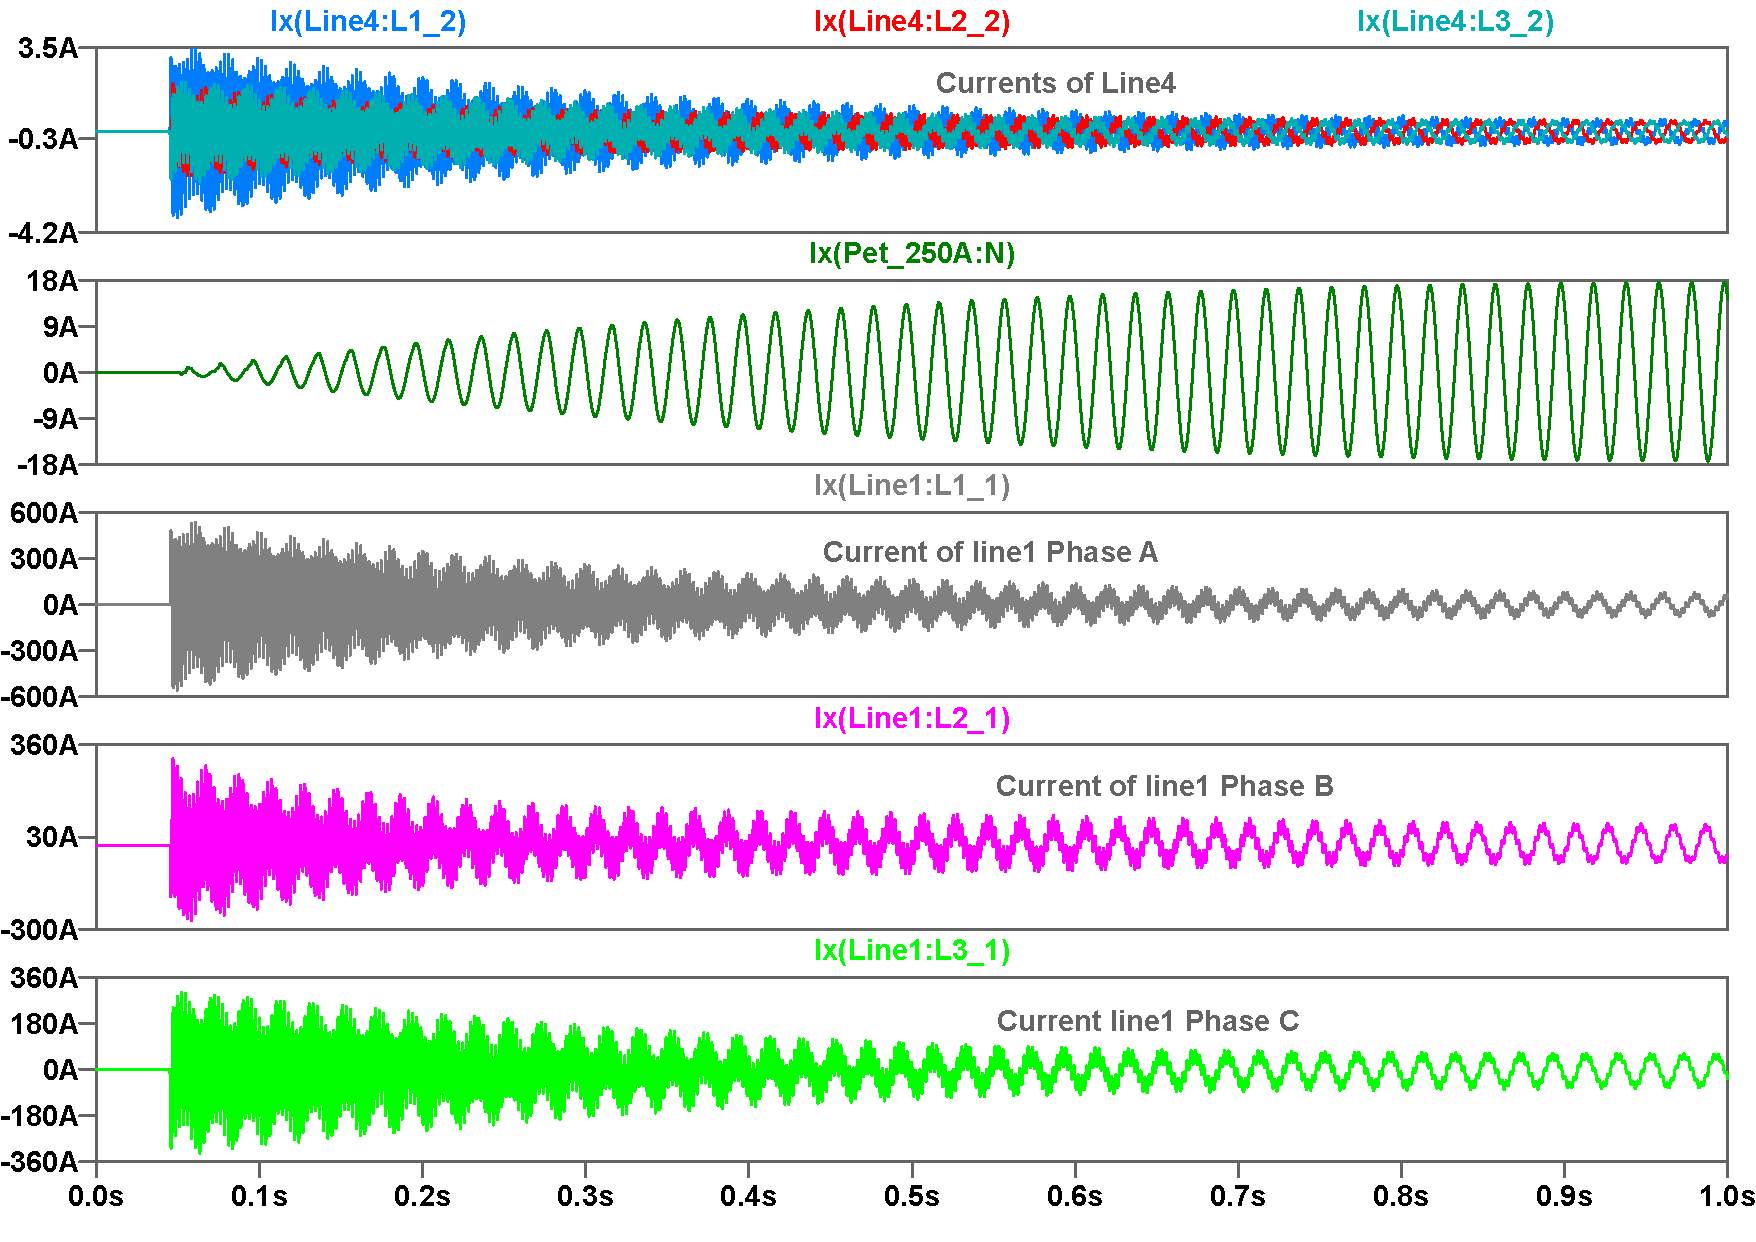
\includegraphics[width=0.90\textwidth]{figures/06_Switching_on_networks/Switching_on_networks_currents_Line1_Line4-case2}
	\caption{Switching on networks currents line1, line4 - case2}
	\label{fig:figure69}
\end{figure}

\begin{figure}[H]
	\centering
	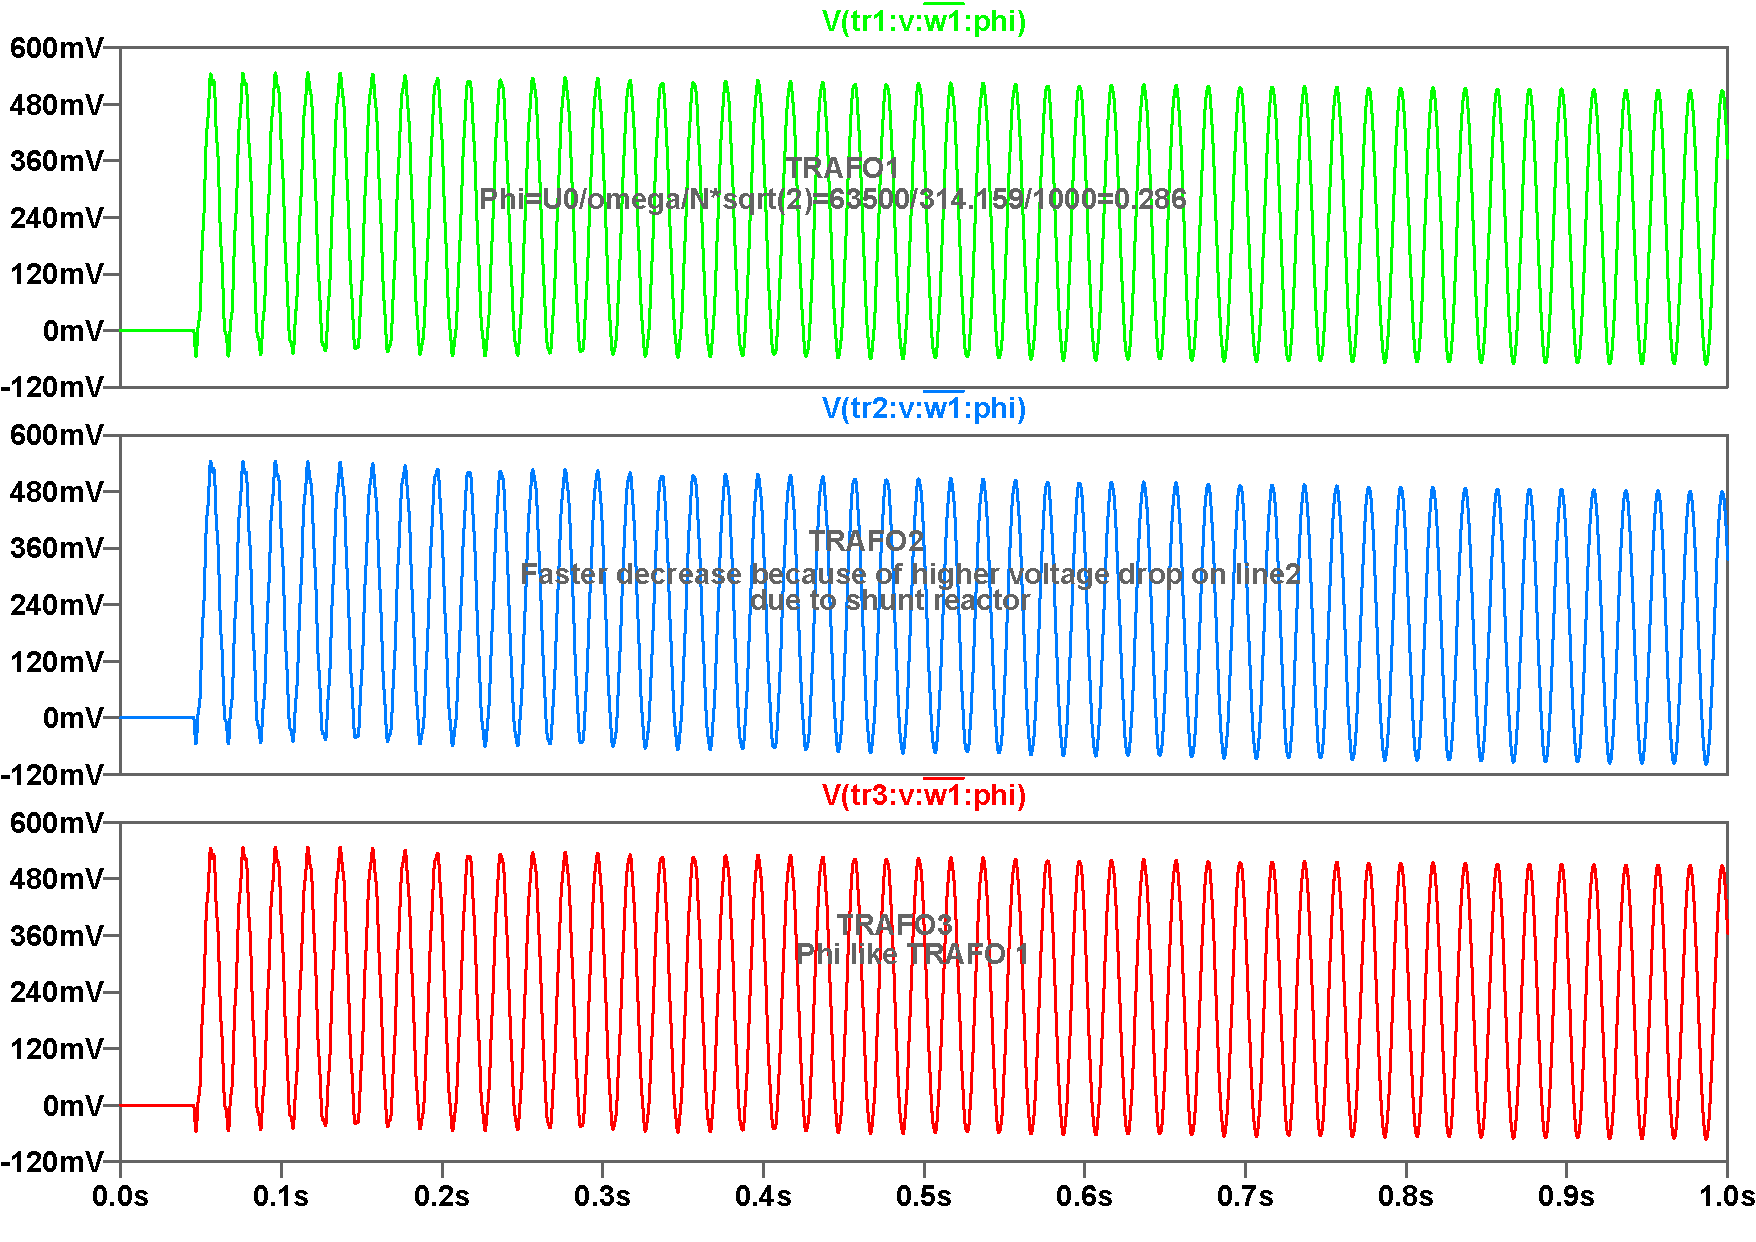
\includegraphics[width=0.90\textwidth]{figures/06_Switching_on_networks/Switching_on_networks_phi-case2}
	\caption{Switching on networks fluxes - case2}
	\label{fig:figure610}
\end{figure}

% Measurement values table for the Power System Simulation book.
% Required packages are already loaded by the central preamble:
% booktabs, tabularx, array, siunitx, xcolor.

\begin{table}[htbp]
  \centering
  \caption{Signal ranges for Case 2. All values are peak values, bus values are multiplied by 1.73/1.414}
  \label{tab:measurement-values-case2}
  \small
  \setlength{\tabcolsep}{3.5pt}
  \renewcommand{\arraystretch}{1.18}
  \begin{tabularx}{\textwidth}{@{}
      >{\raggedright\arraybackslash}p{0.055\textwidth}
      >{\raggedright\arraybackslash}p{0.085\textwidth}
      >{\raggedright\arraybackslash}p{0.095\textwidth}
      >{\raggedright\arraybackslash}p{0.105\textwidth}
      >{\raggedright\arraybackslash}p{0.075\textwidth}
      >{\raggedright\arraybackslash}p{0.075\textwidth}
      Y@{}}
    \toprule
    \textbf{Meas.} &
    \textbf{Grid element} &
    \textbf{Phase} &
    \textbf{Voltage level} &
    \textbf{Min.} &
    \textbf{Max.} &
    \textbf{Notes} \\
    \midrule
    $V$ & Bus0  & Ph A       & \SI{220}{\kilo\volt} & \SI{-229}{\kilo\volt} & \SI{229}{\kilo\volt} & -- \\
    $V$ & Bus1  & Ph A, B, C & \SI{110}{\kilo\volt} & \SI{-200}{\kilo\volt} & \SI{200}{\kilo\volt} & -- \\
    $I$ & HTr1  & Ph A       & \SI{220}{\kilo\volt} & \SI{-520}{\ampere} & \SI{510}{\ampere} & -- \\
    $I$ & HTr1  & Ph B       & \SI{220}{\kilo\volt} & \SI{-170}{\ampere} & \SI{460}{\ampere} & -- \\
    $I$ & HTr1  & Ph C       & \SI{220}{\kilo\volt} & \SI{-470}{\ampere} & \SI{180}{\ampere} & -- \\
    $I$ & KD1   & Ph A       & \SI{110}{\kilo\volt} & \SI{-300}{\ampere} & \SI{300}{\ampere} & Steady state: \SI{300}{\ampere} \\
    $I$ & Tr1   & Ph B       & \SI{110}{\kilo\volt} & \SI{-4}{\ampere} & \SI{26}{\ampere} & Due to Petersen values under zero line \\
    $I$ & Tr2   & Ph B       & \SI{110}{\kilo\volt} & \SI{0}{\ampere} & \SI{25}{\ampere} & Due to KD: faster decrease of current \\
    $I$ & Tr3   & Ph A      & \SI{110}{\kilo\volt} & \SI{0}{\ampere} & \SI{25}{\ampere} & -- \\
    $I$ & Line4 & Ph A & \SI{110}{\kilo\volt} & \SI{-3.5}{\ampere} & \SI{3.5}{\ampere} & Small capacitive inrush current due to overhead line \\
    $I$ & Line1 & Ph A & \SI{110}{\kilo\volt} & \SI{-500}{\ampere} & \SI{500}{\ampere} & High capacitive inrush current due to cable \\
    $I$ & Line1 & Ph B, C & \SI{110}{\kilo\volt} & \SI{-300}{\ampere} & \SI{300}{\ampere} & High capacitive inrush current due to cable \\
    $I$ & Pet1 & Ph N & \SI{110}{\kilo\volt} & \SI{-18}{\ampere} & \SI{18}{\ampere} & Longtime value very small \\
    $V$ & Pet1 & Ph N & \SI{110}{\kilo\volt} & \SI{-4.5}{\kilo\volt} & \SI{4.5}{\kilo\volt} & Longtime value very small \\
    $\Phi$ & Tr1 & Ph B, C   & \SI{110}{\kilo\volt} & \SI{0}{\weber} & \SI{0.54}{\weber} & Nominal flux: \SI{0.288}{\weber} \\
    \bottomrule
  \end{tabularx}
\end{table}



\section{Case 3: Closing at Voltage Zero with Full Residual Flux}
\label{sec:network-closing-residual-flux}

Set \texttt{psi\_0=1}. Phase A then carries a very large combined magnetizing
current from the medium-voltage transformers. Measured on the
\SI{220}{\kilo\volt} side of the main transformer, the peak is approximately
\SI{920}{\ampere}. This exceeds the rated peak current of
approximately $\sqrt{2}\cdot\SI{525}{\ampere}=\SI{742}{\ampere}$.

With unfavourable full residual flux, the Phase A flux can theoretically approach three times its normal peak. The theoretical peak would therefore be approximately \SI{8.64}{\weber}.
This theoretical peak cannot be achieved in practice. The reason is, on the one hand, the reduced voltage caused by the high current and external and internal voltage drops. The attainable flux is reduced by voltage drops caused by the high current, as well as by secondary-winding currents and leakage flux. 
The fast decrease of the currents is due to the nonlinear characteristic of the magnetizing curve. 

The neutral-point voltage across the Petersen coil of transformer 1 initially rises to a high value (about nominal voltage) and then
decays slowly. The cause is the large asymmetry of the phase magnetizing
currents, which also makes the phase-to-earth voltages asymmetric. The
line-to-line voltages are much less affected. If the simulation is extended to
\SI{60}{\second}, the magnetizing currents approach their small steady-state
values and the Petersen-coil voltage settles to approximately
\SIrange{1}{2}{\kilo\volt}.

The very high neutral displacement voltage, which reaches approximately the nominal phase-to-earth voltage, which also slowly builds up at the neutral point of the main transformer, causes a highly asymmetrical voltage in Phase B of the grid. This voltage first rises, then drops to nearly half the rated voltage, and then rises again. 

For Waveforms see figures \ref{fig:figure611}-\ref{fig:figure614}. 
For Measurement values and signal ranges see table: \ref{tab:measurement-values-case3}.\\ 

\begin{figure}[H]
	\centering
	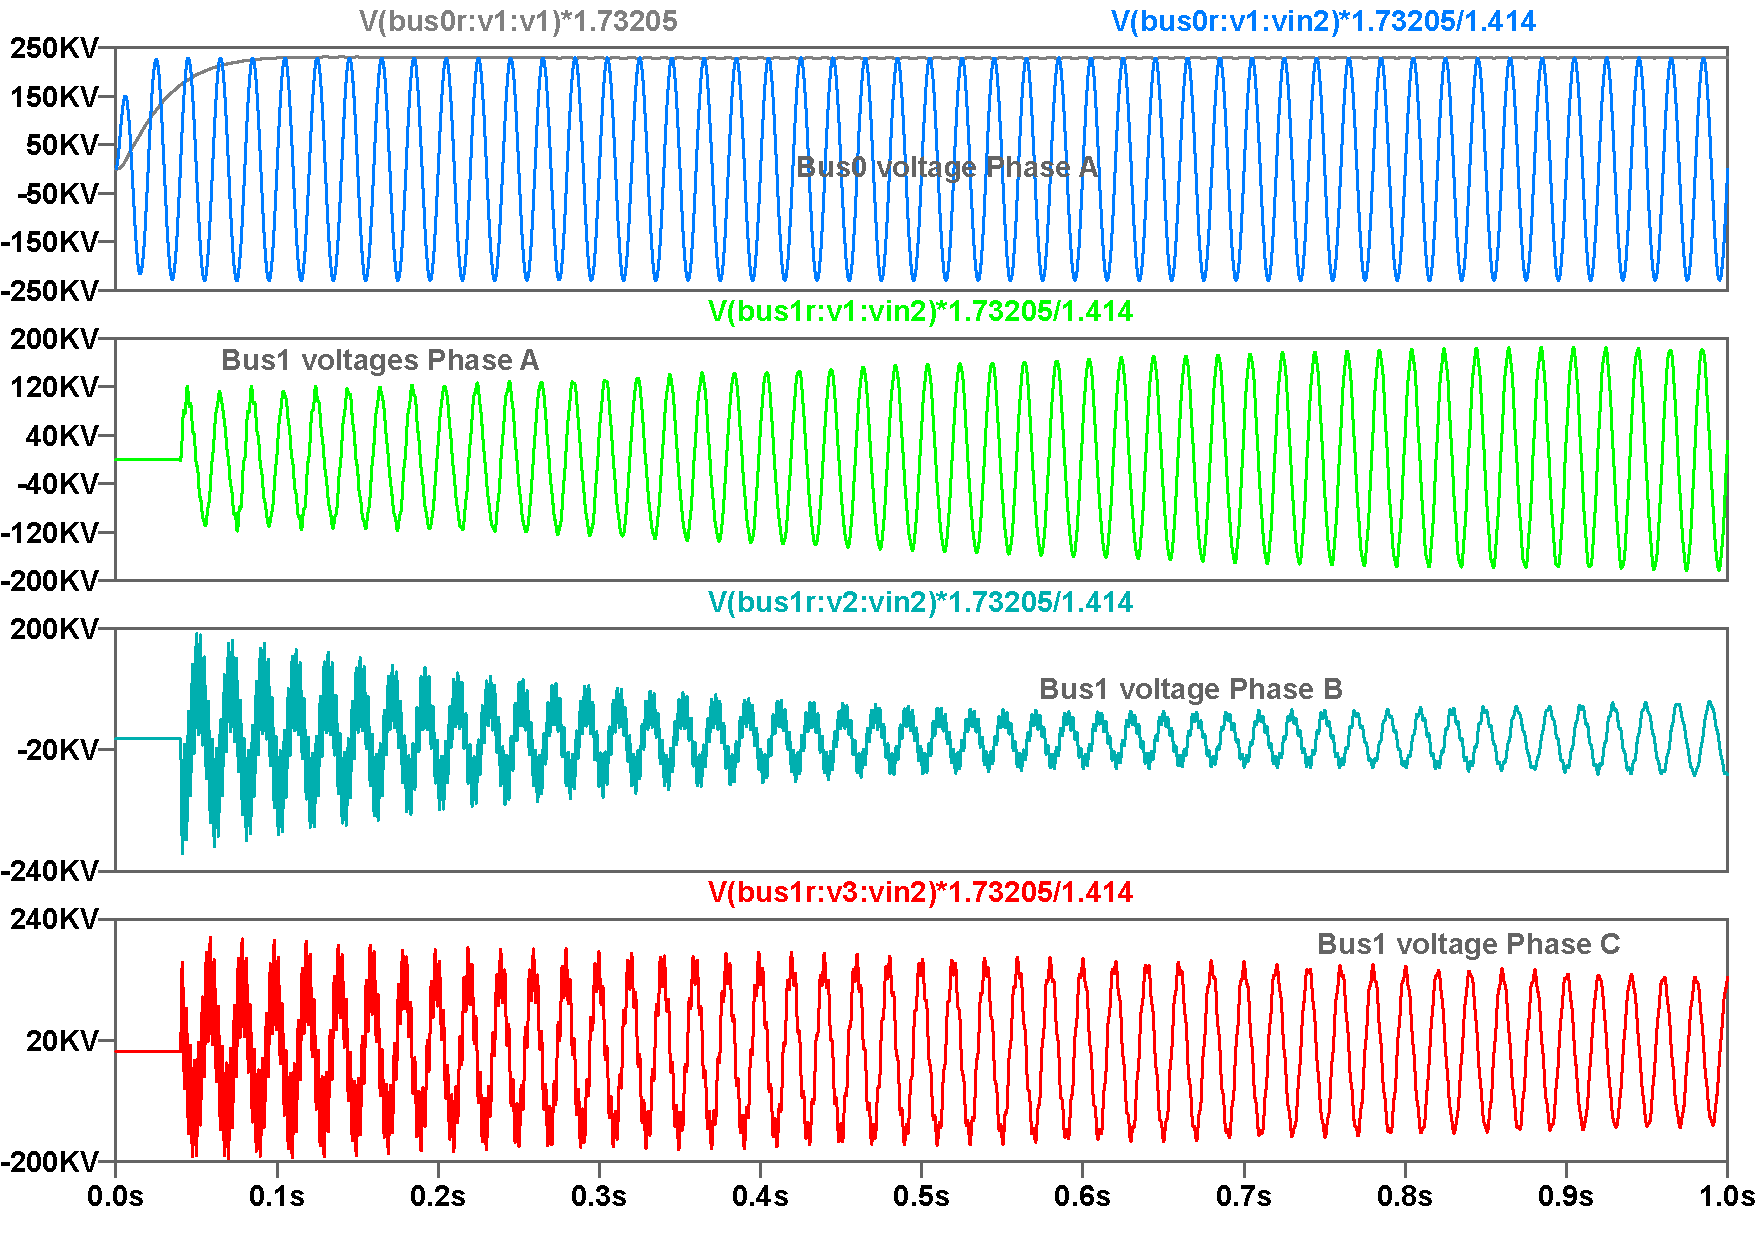
\includegraphics[width=0.90\textwidth]{figures/06_Switching_on_networks/Switching_on_networks_Bus0_Bus1_voltages-case3}
	\caption{Switching on networks voltages - case3}
	\label{fig:figure611}
\end{figure}

\begin{figure}[H]
	\centering
	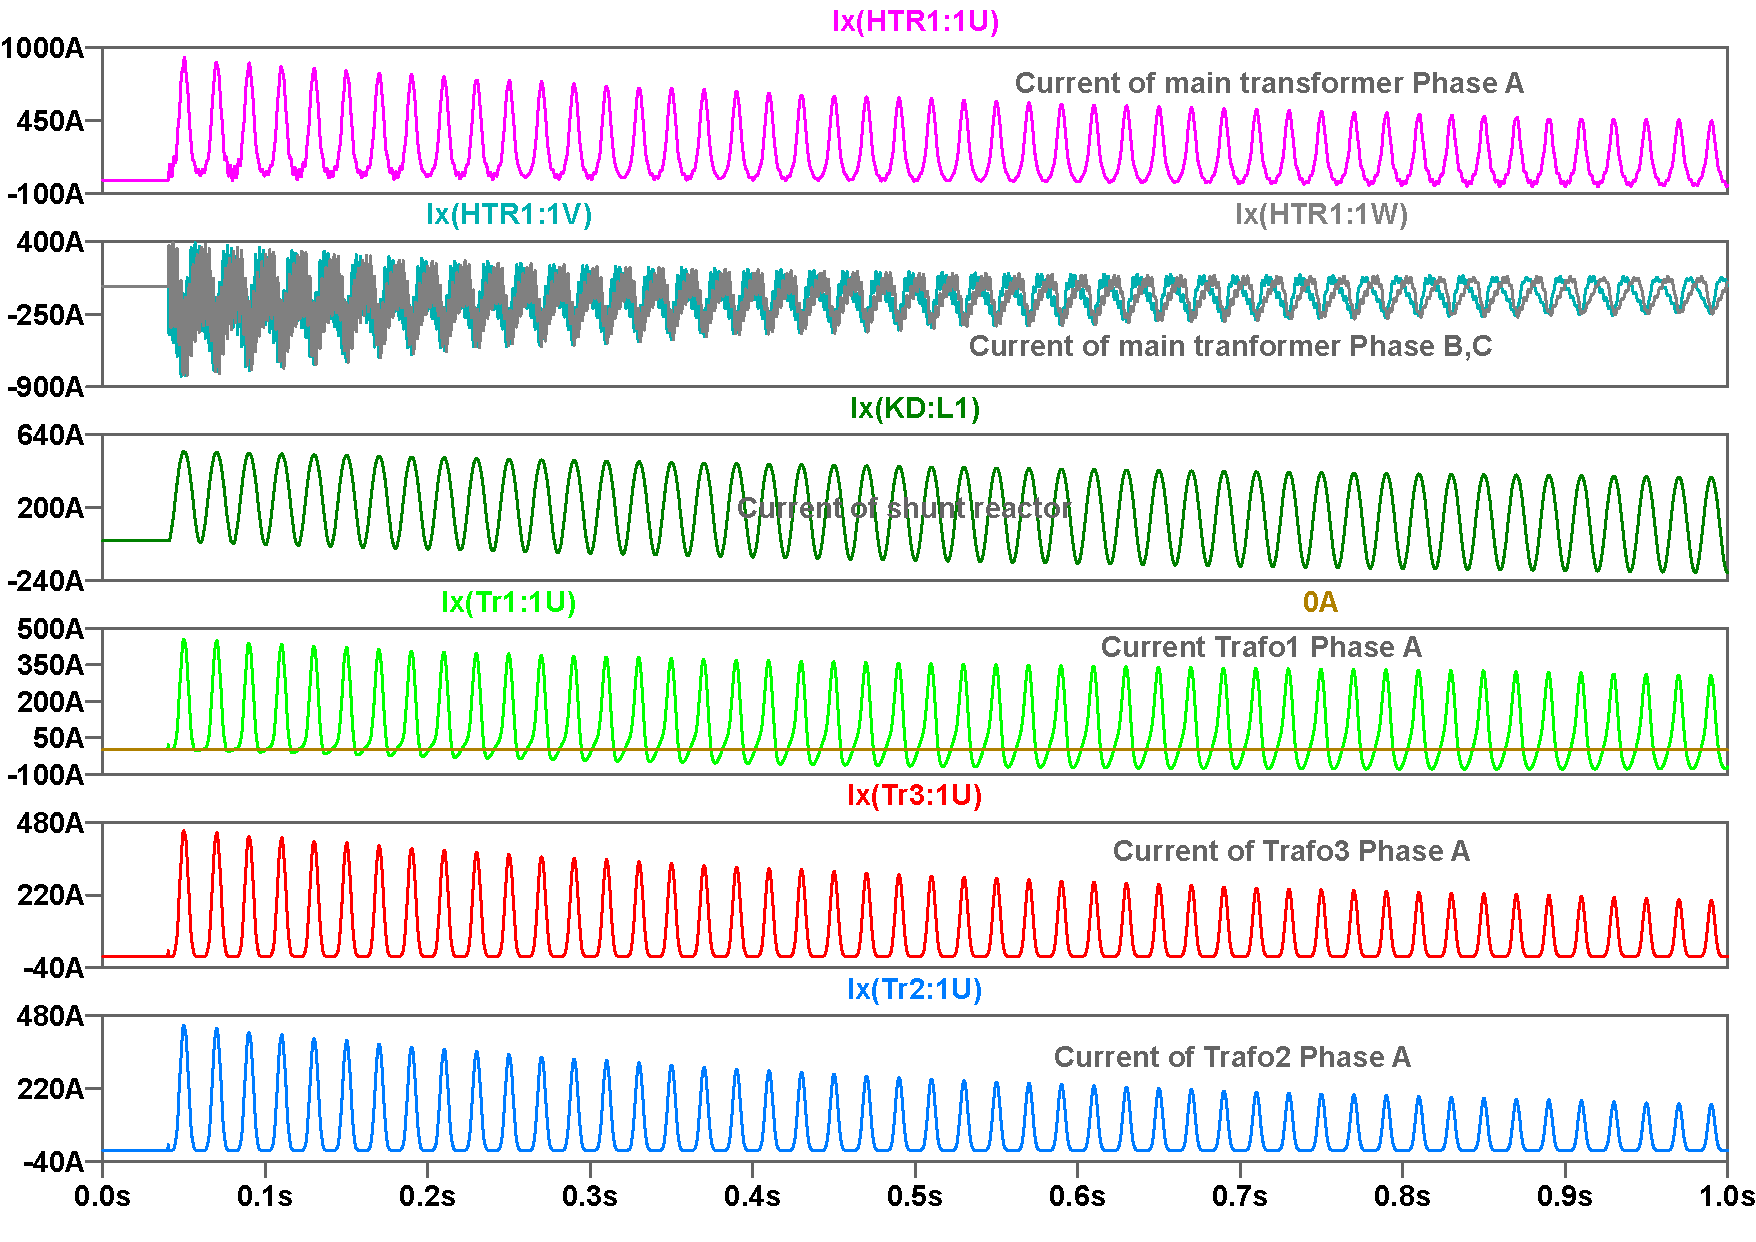
\includegraphics[width=0.90\textwidth]{figures/06_Switching_on_networks/Switching_on_networks_currents-case3}
	\caption{Switching on networks currents - case3}
	\label{fig:figure612}
\end{figure}

\begin{figure}[H]
	\centering
	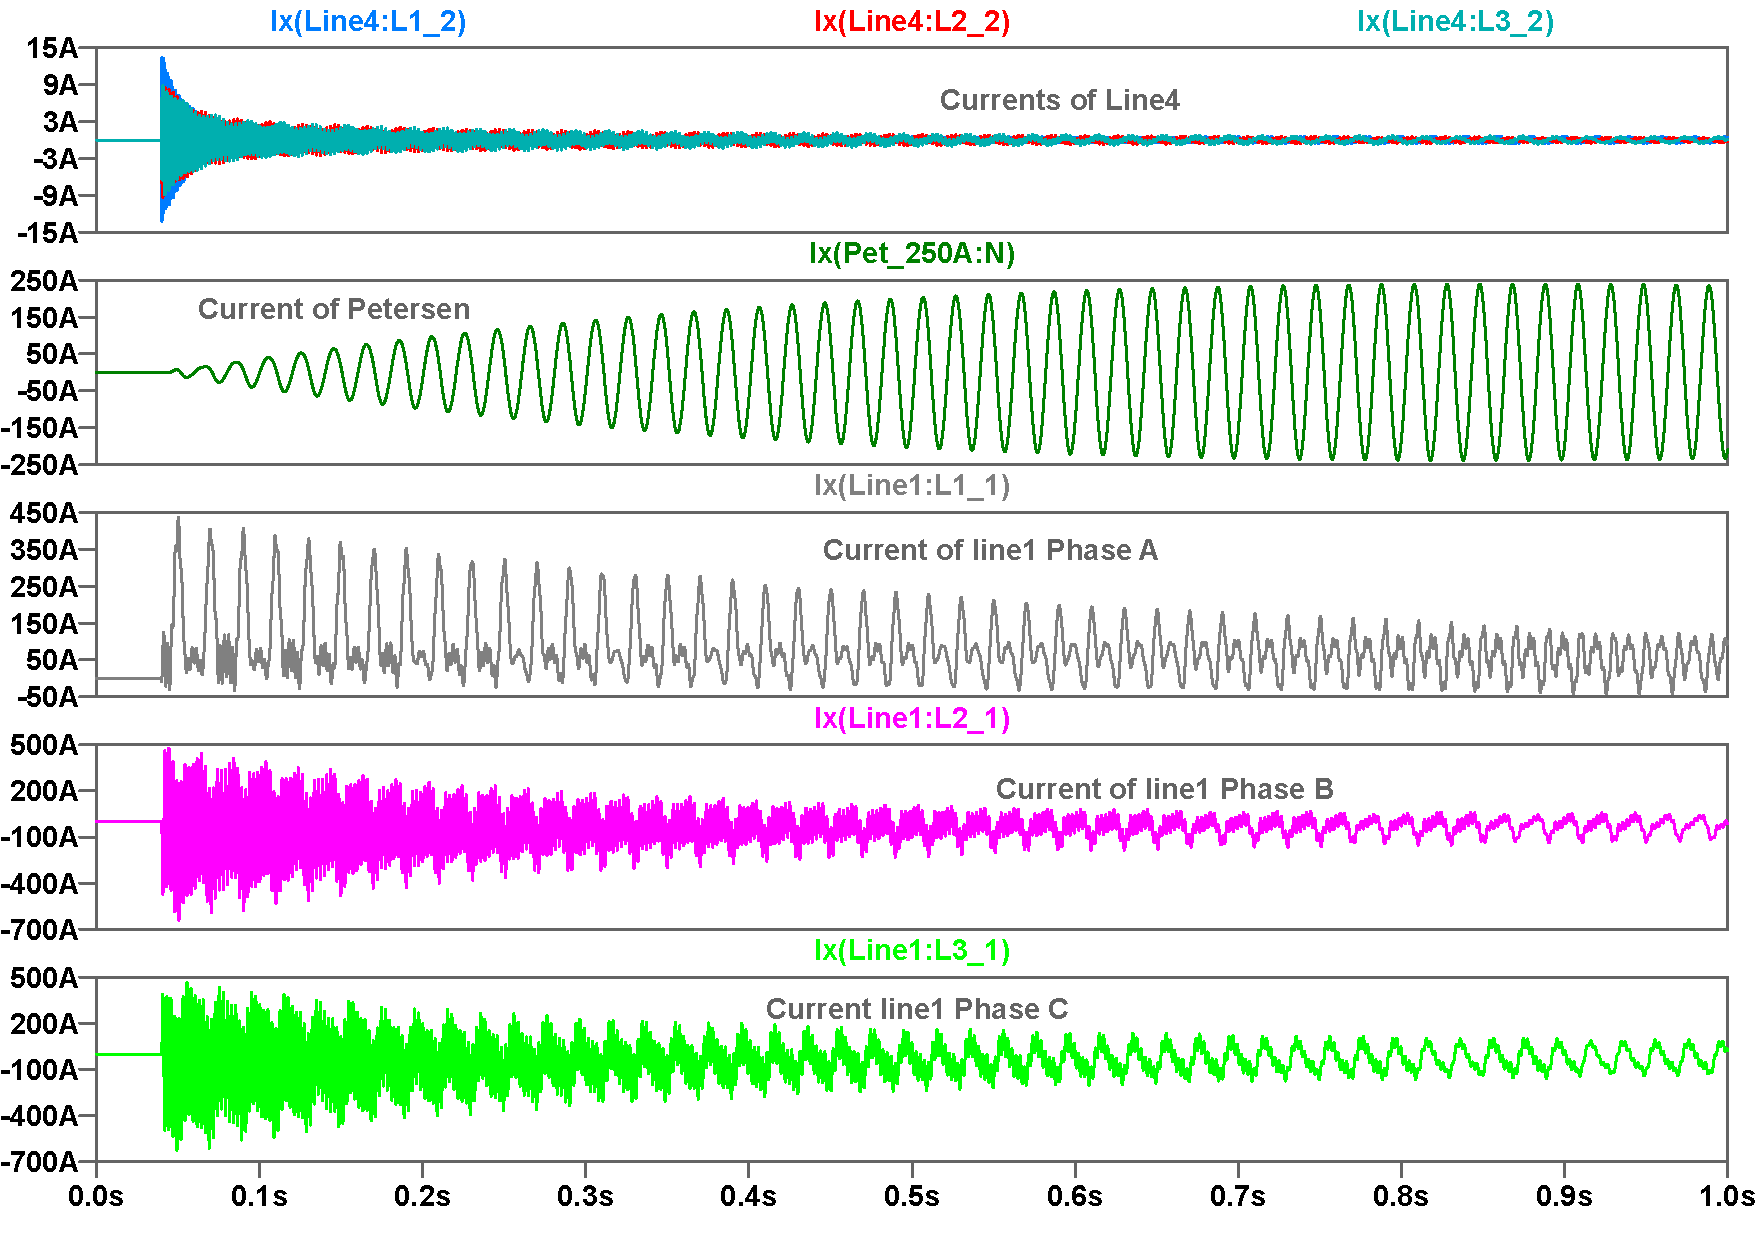
\includegraphics[width=0.90\textwidth]{figures/06_Switching_on_networks/Switching_on_networks_currents_Line1_Line4-case3}
	\caption{Switching on networks currents line1, line4 - case3}
	\label{fig:figure613}
\end{figure}

\begin{figure}[H]
	\centering
	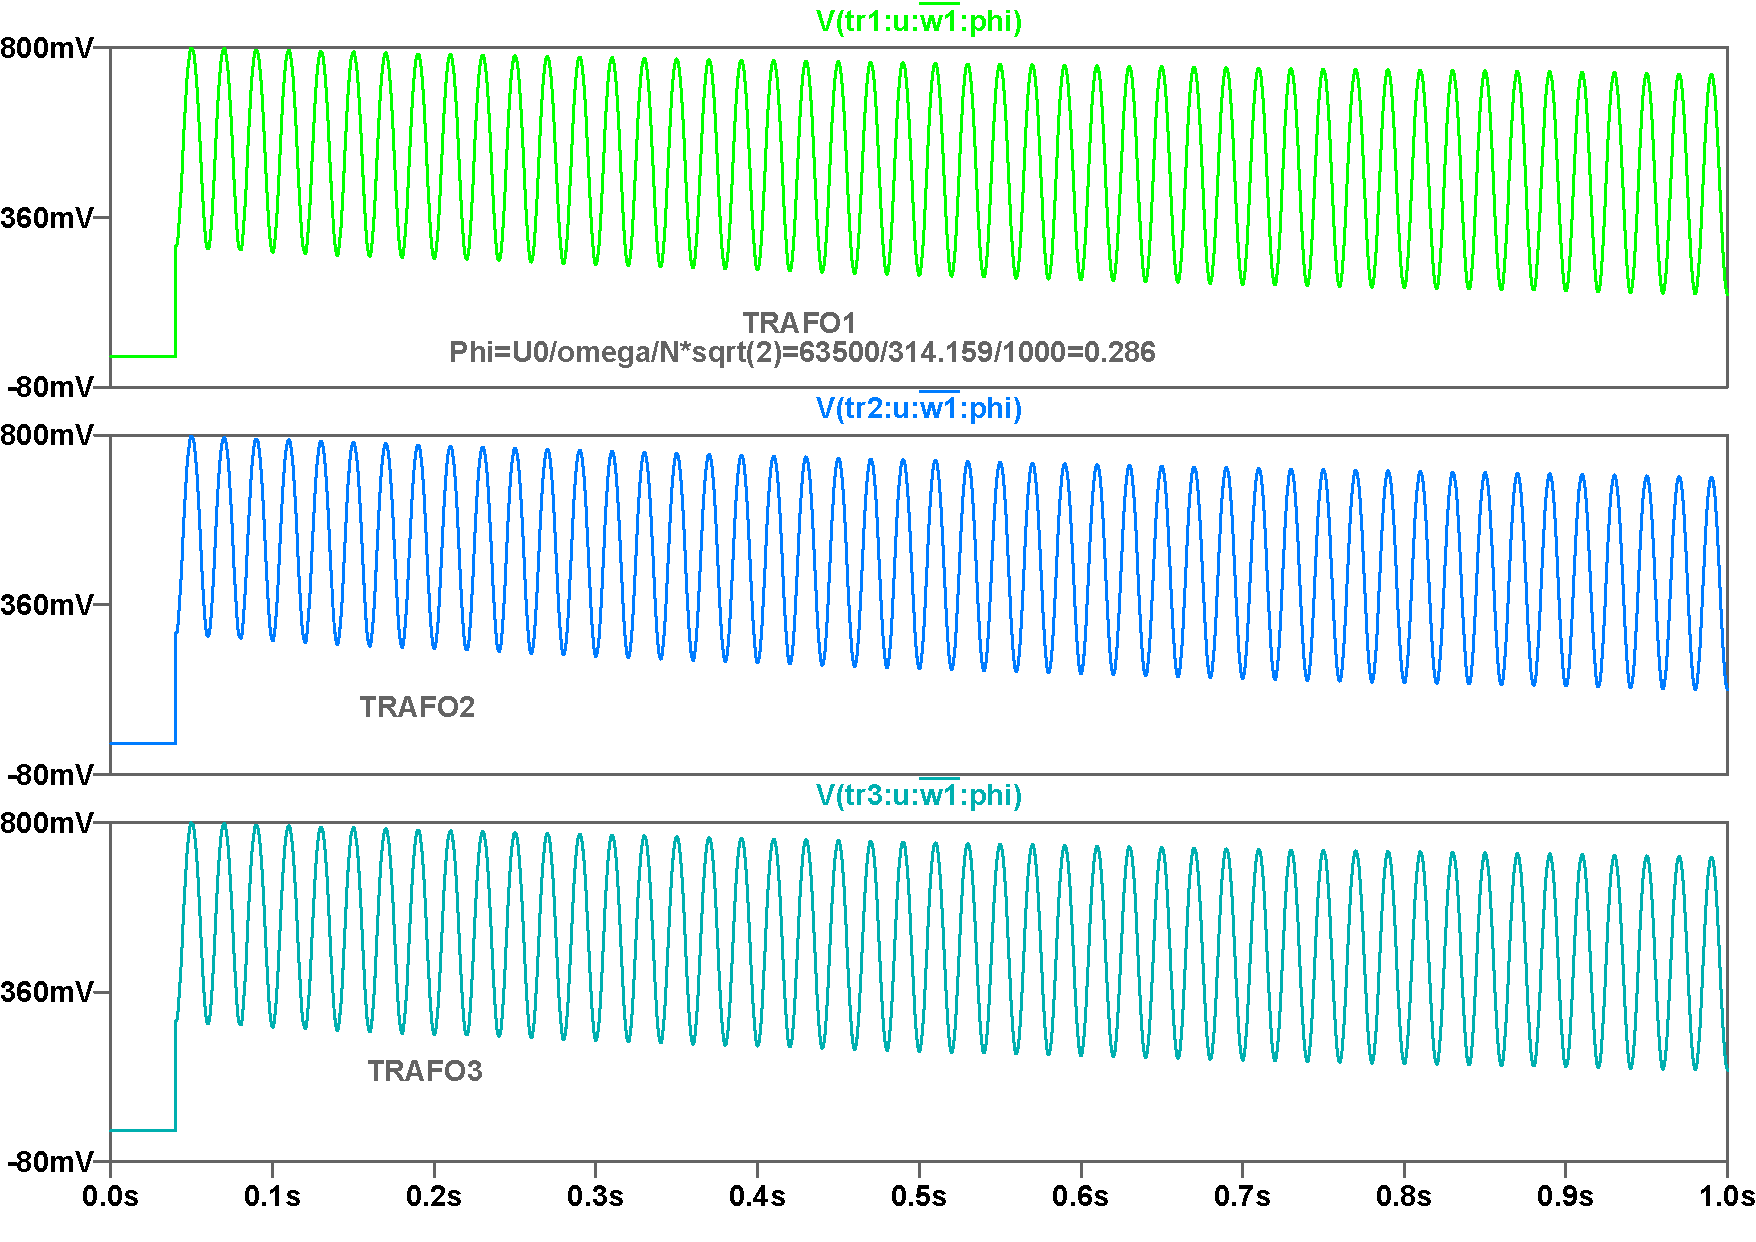
\includegraphics[width=0.90\textwidth]{figures/06_Switching_on_networks/Switching_on_networks_phi-case3}
	\caption{Switching on networks fluxes - case3}
	\label{fig:figure614}
\end{figure}

% Measurement values table for the Power System Simulation book.
% Required packages are already loaded by the central preamble:
% booktabs, tabularx, array, siunitx, xcolor.

\begin{table}[htbp]
  \centering
  \caption{Signal ranges for Case 3. All values are peak values, bus values are multiplied by 1.73/1.414}
  \label{tab:measurement-values-case3}
  \small
  \setlength{\tabcolsep}{3.5pt}
  \renewcommand{\arraystretch}{1.18}
  \begin{tabularx}{\textwidth}{@{}
      >{\raggedright\arraybackslash}p{0.055\textwidth}
      >{\raggedright\arraybackslash}p{0.085\textwidth}
      >{\raggedright\arraybackslash}p{0.095\textwidth}
      >{\raggedright\arraybackslash}p{0.105\textwidth}
      >{\raggedright\arraybackslash}p{0.075\textwidth}
      >{\raggedright\arraybackslash}p{0.075\textwidth}
      Y@{}}
    \toprule
    \textbf{Meas.} &
    \textbf{Grid element} &
    \textbf{Phase} &
    \textbf{Voltage level} &
    \textbf{Min.} &
    \textbf{Max.} &
    \textbf{Notes} \\
    \midrule
    $V$ & Bus0  & Ph A       & \SI{220}{\kilo\volt} & \SI{-229}{\kilo\volt} & \SI{229}{\kilo\volt} & -- \\
    $V$ & Bus1  & Ph A,    & \SI{110}{\kilo\volt} & \SI{-120}{\kilo\volt} & \SI{120}{\kilo\volt} & Startup values low and later higher \\
    $V$ & Bus1  & Ph B     & \SI{110}{\kilo\volt} & \SI{-200}{\kilo\volt} & \SI{200}{\kilo\volt} & Startup values high and later much smaller than higher again, Steady state: \SI{114}{\kilo\volt} \\
    $V$ & Bus1  & Ph C     & \SI{110}{\kilo\volt} & \SI{-200}{\kilo\volt} & \SI{200}{\kilo\volt} & Steady state: \SI{114}{\kilo\volt} RMS \\
    $I$ & HTr1  & Ph A       & \SI{220}{\kilo\volt} & \SI{0}{\ampere} & \SI{920}{\ampere} & -- \\
    $I$ & HTr1  & Ph B       & \SI{220}{\kilo\volt} & \SI{-800}{\ampere} & \SI{400}{\ampere} & -- \\
    $I$ & HTr1  & Ph C       & \SI{220}{\kilo\volt} & \SI{-800}{\ampere} & \SI{400}{\ampere} & -- \\
    $I$ & KD1   & Ph A       & \SI{110}{\kilo\volt} & \SI{0}{\ampere} & \SI{540}{\ampere} & Steady state: \SI{300}{\ampere} \\
    $I$ & Tr1   & Ph A       & \SI{110}{\kilo\volt} & \SI{-80}{\ampere} & \SI{450}{\ampere} & Due to Petersen values under zero line \\
    $I$ & Tr2   & Ph A       & \SI{110}{\kilo\volt} & \SI{0}{\ampere} & \SI{450}{\ampere} & Due to KD1: faster decrease of current \\
    $I$ & Tr3   & Ph A      & \SI{110}{\kilo\volt} & \SI{0}{\ampere} & \SI{450}{\ampere} & -- \\
    $I$ & Line4 & Ph A & \SI{110}{\kilo\volt} & \SI{-13}{\ampere} & \SI{13}{\ampere} & Small capacitive inrush current  \\
    $I$ & Line1 & Ph A & \SI{110}{\kilo\volt} & \SI{-20}{\ampere} & \SI{440}{\ampere} & High capacitive inrush current due to cable \\
    $I$ & Line1 & Ph B, C & \SI{110}{\kilo\volt} & \SI{-500}{\ampere} & \SI{500}{\ampere} & High capacitive inrush current due to cable \\
    $I$ & Pet1 & Ph N & \SI{110}{\kilo\volt} & \SI{-240}{\ampere} & \SI{240}{\ampere} & Longtime value very small \\
    $V$ & Pet1 & Ph N & \SI{110}{\kilo\volt} & \SI{-60}{\kilo\volt} & \SI{60}{\kilo\volt} & Longtime value very small \\
    $\Phi$ & Tr1 & Ph A, B, C   & \SI{110}{\kilo\volt} & \SI{0}{\weber} & \SI{0.8}{\weber} & Nominal flux: \SI{0.288}{\weber} \\
    \bottomrule
  \end{tabularx}
\end{table}


\section{Case 4: Main-Transformer Tap Position \texttt{L+13}}
\label{sec:network-tap-l13}

Set \texttt{L=13}. The changed tap position reduces the secondary voltage of the main transformer. The currents and maximum flux values at \SI{500}{\milli\weber} are also lower than in Case 1. The Phase A voltage at bus1 reaches approximately 100 kV peak and contains almost no 400 Hz component associated with the capacitive charging transient. The peak voltages in phases B and C are approximately 180 kV. The Petersen-coil current is approximately 2.5 A, and the current in line 4 is similar to that in Case 1. In line 1, the peak currents are approximately 500 A in phases B and C and 100 A in phase A. The peak transformer inrush currents are approximately 11.5 A, substantially lower than in Case 1 because the maximum core flux is reduced. 
For Schematic and waveforms see figures \ref{fig:figure615}- \ref{fig:figure619}. 
For measured values and signal ranges, see Table \ref{tab:measurement-values-case4}.
An FFT shows that the dominant resonance shifts from approximately
\SI{400}{\hertz} to \SI{450}{\hertz}. 
With voltage ratio = 220kV/97kV=2.268 and t=2.268*2.268=5.14. Compared to calculation \ref{calc:whole-network-resonance}  the resonant frequency is

%The tap position changes the effective
%transformation ratio and therefore the transformer reactance referred to the
%secondary side. To compare both cases in one simulation, add
%With voltage ratio = 220kV/97kV=2.268 and t=2.268*2.268=5.14 the resonant frequency compared to

\begin{calculation}{Dominant cable-network resonance}{whole-network-resonance2}
	\begin{align}
		L_{\mathrm{eq}}&=\frac{L_{\mathrm{net}}}{5.14}
		+\frac{L_{\mathrm{Tr}}}{5.14}
		=\frac{\SI{0.0077}{\henry}+\SI{0.154}{\henry}}{5.14}
		=\SI{0.0314}{\henry},\\
		C&=\SI{4000}{\nano\farad},\\
		f_{\mathrm r}&=\frac{1}{2\pi\sqrt{L_{\mathrm{eq}}C}}
		\approx\boxed{\SI{448.8}{\hertz}}.
	\end{align}
\end{calculation}


\begin{figure}[H]
	\centering
	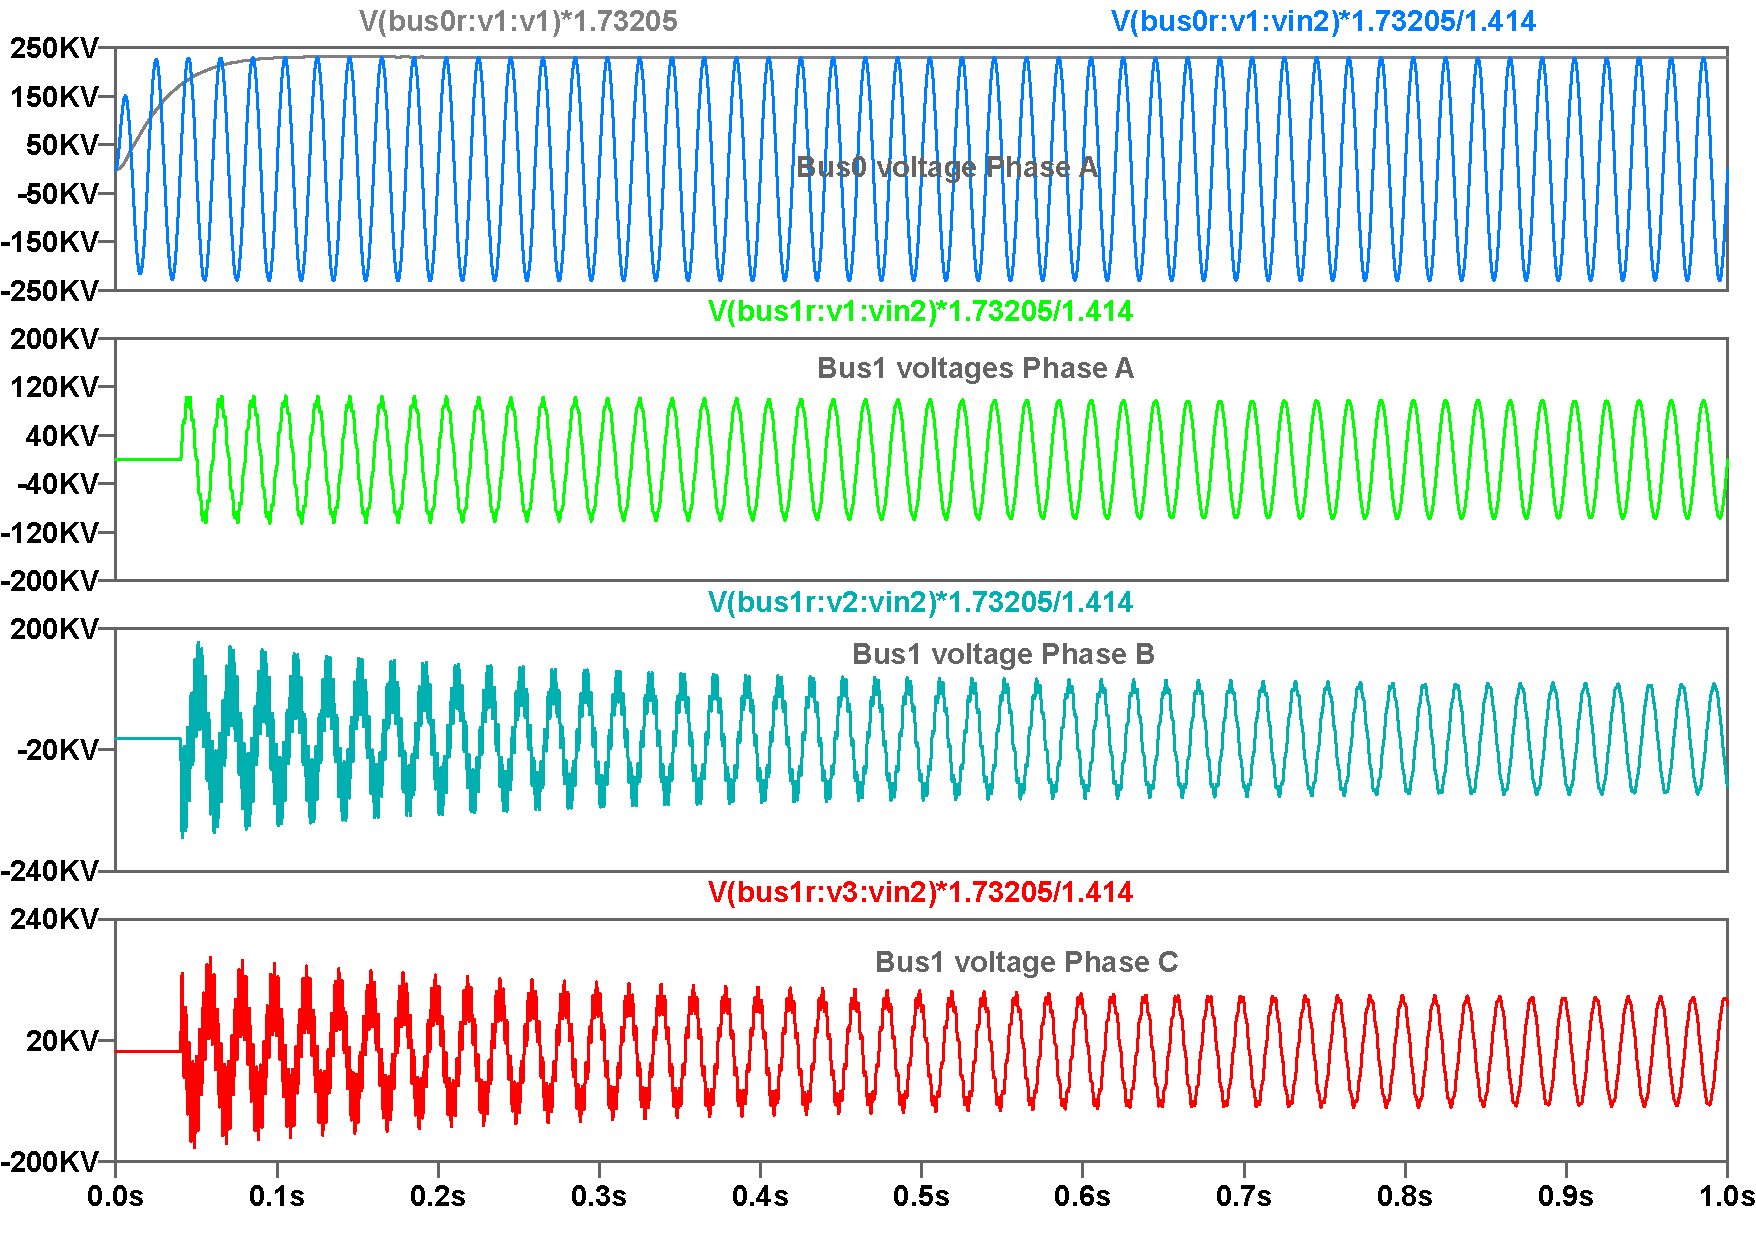
\includegraphics[width=0.90\textwidth]{figures/06_Switching_on_networks/Switching_on_networks_Bus0_Bus1_voltages-case4}
	\caption{Switching on networks voltages - case4}
	\label{fig:figure615}
\end{figure}

\begin{figure}[H]
	\centering
	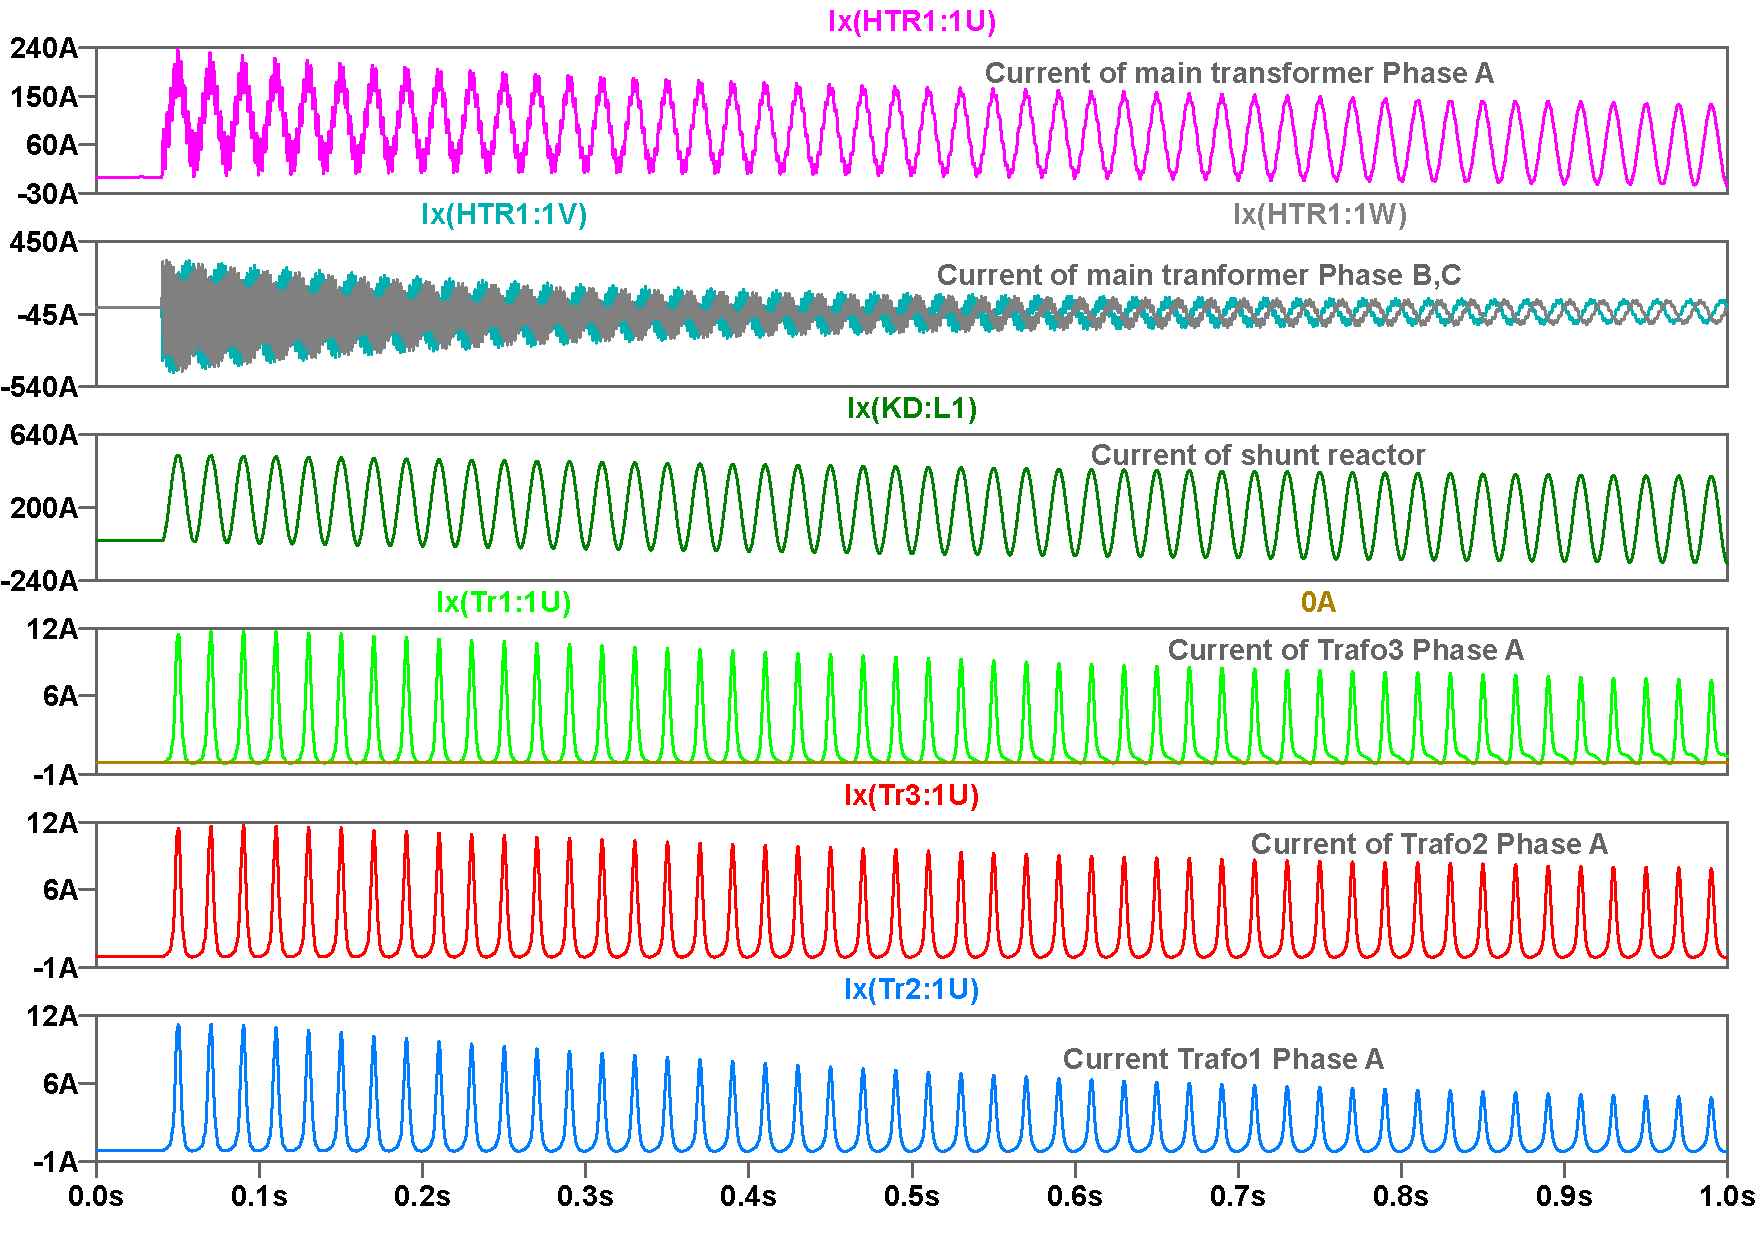
\includegraphics[width=0.90\textwidth]{figures/06_Switching_on_networks/Switching_on_networks_currents-case4}
	\caption{Switching on networks currents - case4}
	\label{fig:figure616}
\end{figure}

\begin{figure}[H]
	\centering
	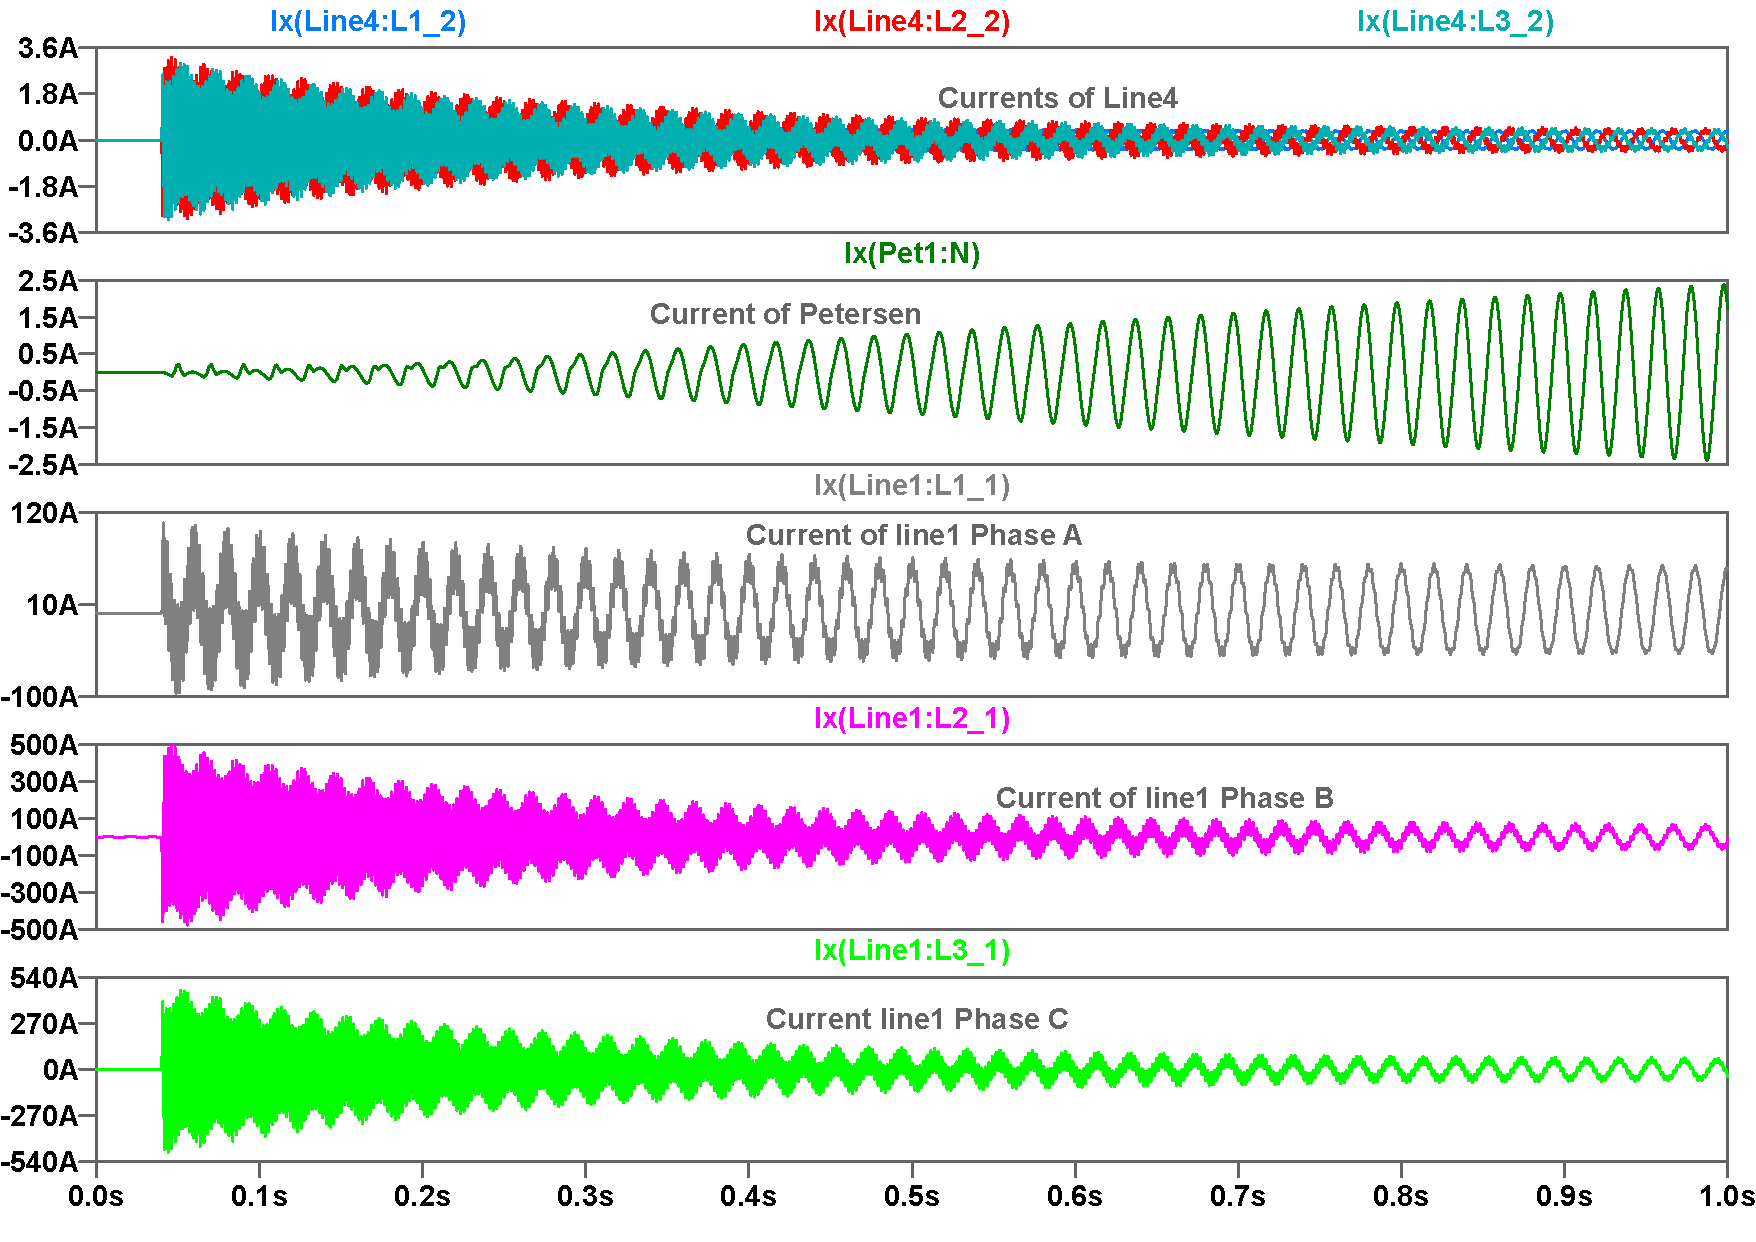
\includegraphics[width=0.90\textwidth]{figures/06_Switching_on_networks/Switching_on_networks_currents_Line1_Line4-case4}
	\caption{Switching on networks currents line1, line4 - case4}
	\label{fig:figure617}
\end{figure}

\begin{figure}[H]
	\centering
	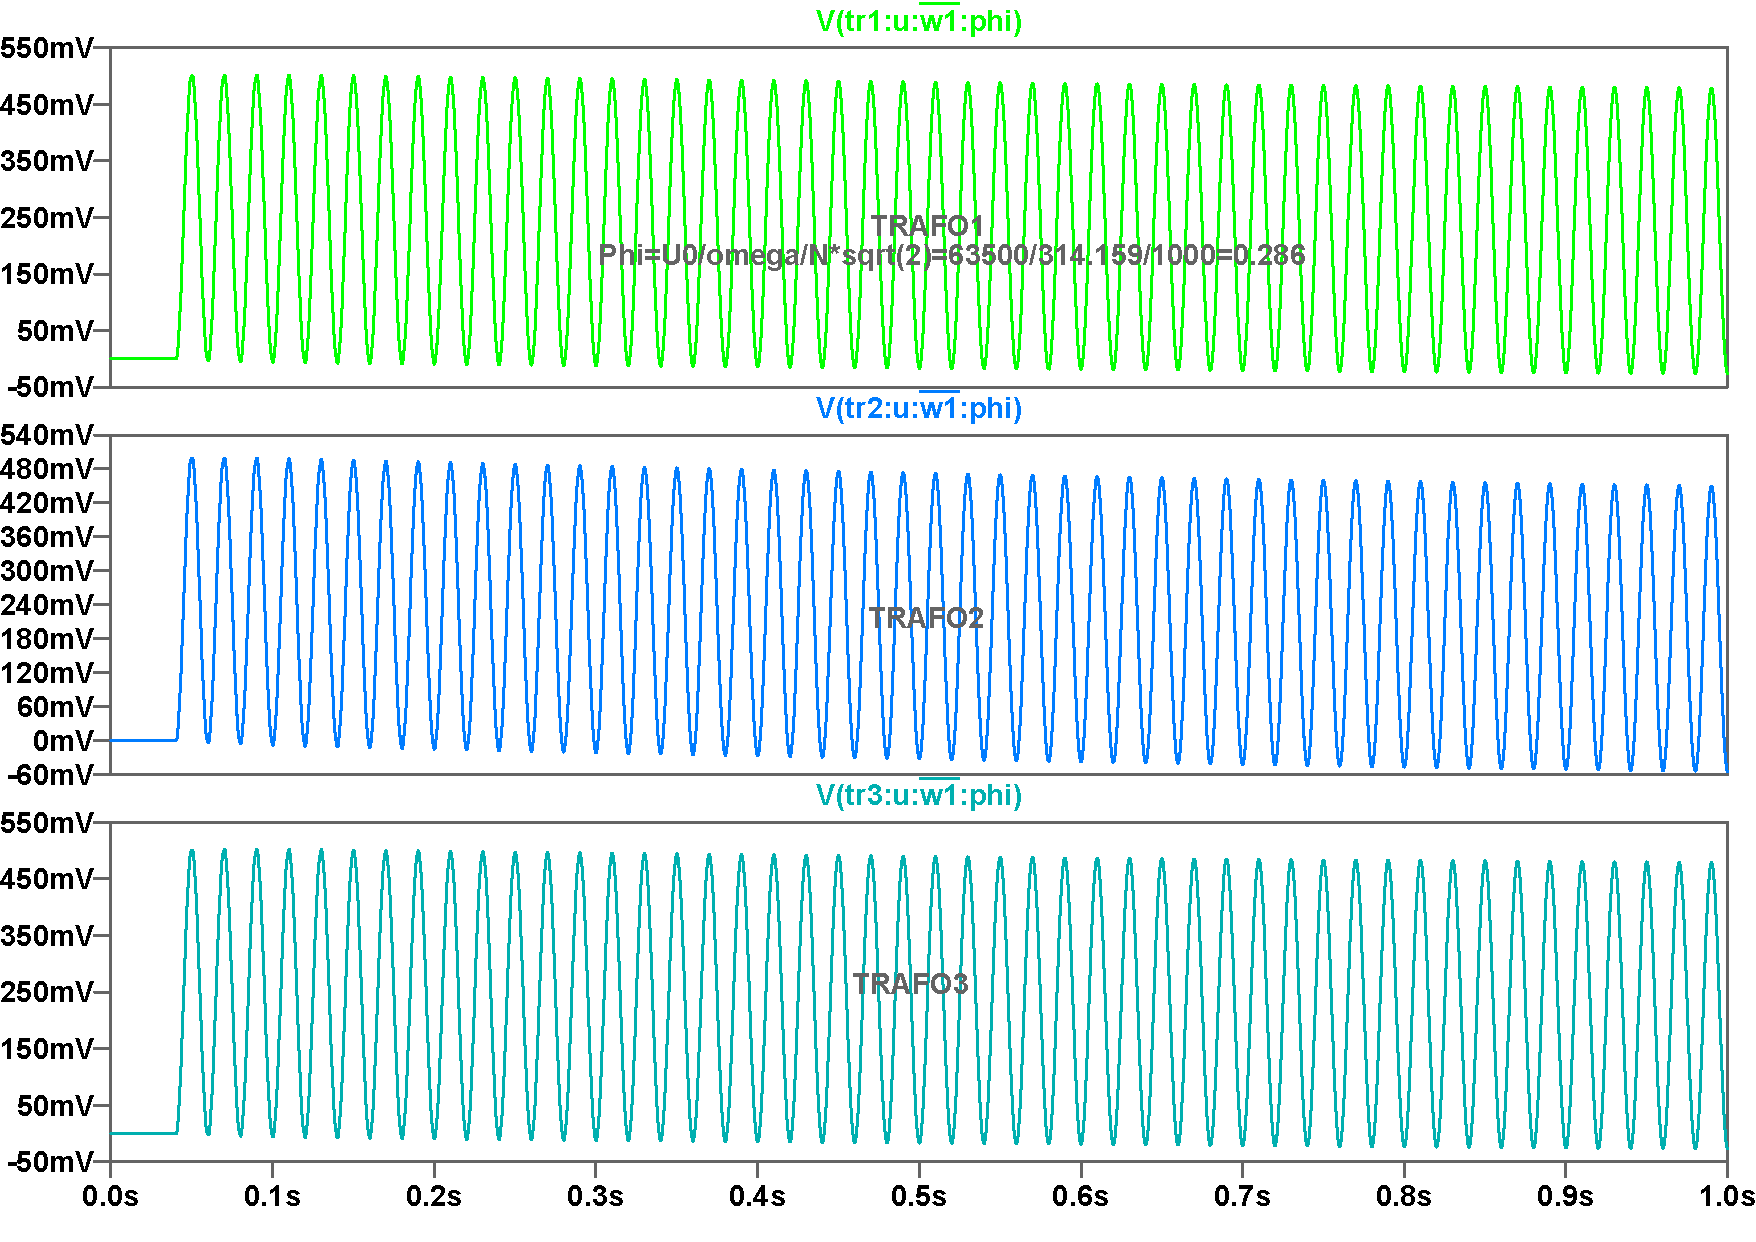
\includegraphics[width=0.90\textwidth]{figures/06_Switching_on_networks/Switching_on_networks_phi-case4}
	\caption{Switching on networks fluxes - case4}
	\label{fig:figure618}
\end{figure}

\begin{figure}[H]
	\centering
	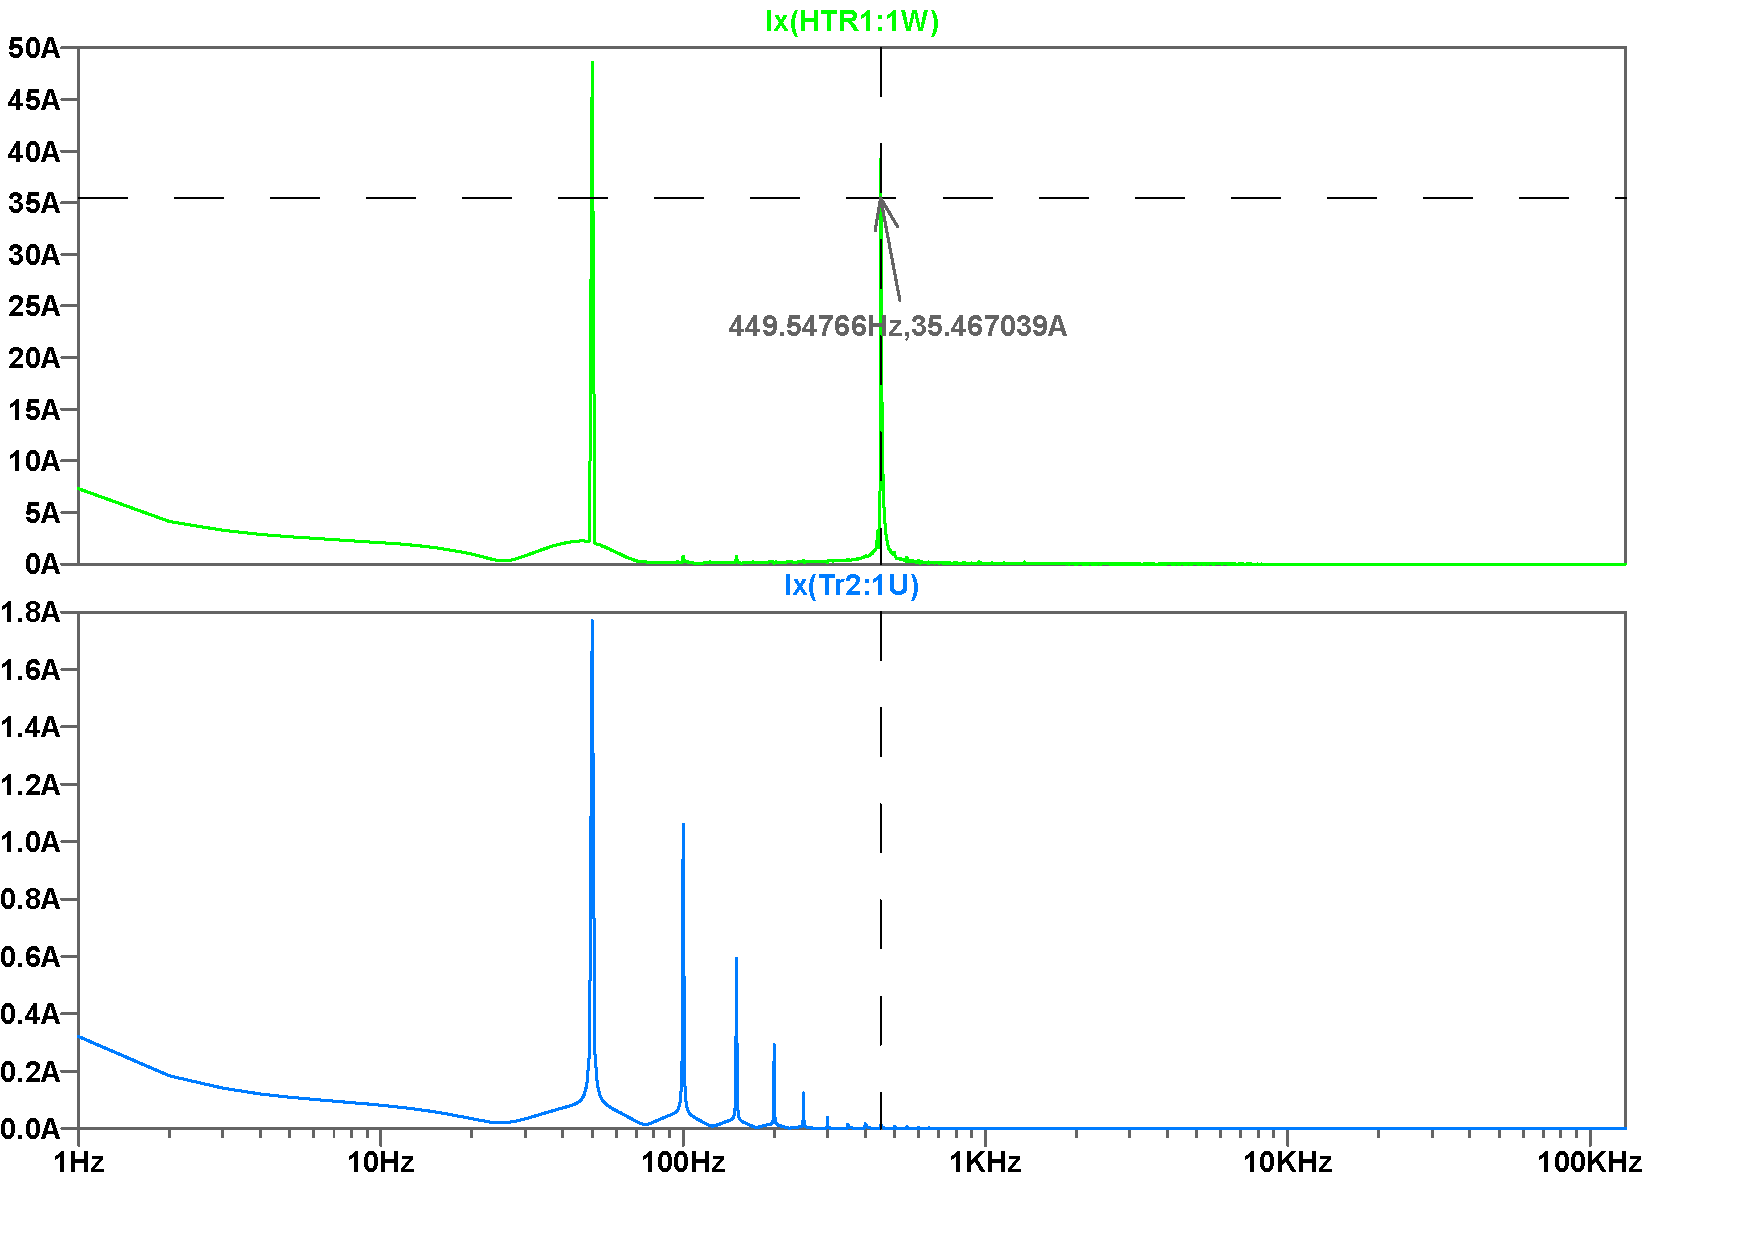
\includegraphics[width=0.90\textwidth]{figures/06_Switching_on_networks/Switching_on_networks_FFT_Transformer-case4}
	\caption{Switching on networks FFT - case4}
	\label{fig:figure619}
\end{figure}

% Measurement values table for the Power System Simulation book.
% Required packages are already loaded by the central preamble:
% booktabs, tabularx, array, siunitx, xcolor.

\begin{table}[htbp]
  \centering
  \caption{Signal ranges for Case 4. All values are peak values, bus values are multiplied by 1.73/1.414}
  \label{tab:measurement-values-case4}
  \small
  \setlength{\tabcolsep}{3.5pt}
  \renewcommand{\arraystretch}{1.18}
  \begin{tabularx}{\textwidth}{@{}
      >{\raggedright\arraybackslash}p{0.055\textwidth}
      >{\raggedright\arraybackslash}p{0.085\textwidth}
      >{\raggedright\arraybackslash}p{0.095\textwidth}
      >{\raggedright\arraybackslash}p{0.105\textwidth}
      >{\raggedright\arraybackslash}p{0.075\textwidth}
      >{\raggedright\arraybackslash}p{0.075\textwidth}
      Y@{}}
    \toprule
    \textbf{Meas.} &
    \textbf{Grid element} &
    \textbf{Phase} &
    \textbf{Voltage level} &
    \textbf{Min.} &
    \textbf{Max.} &
    \textbf{Notes} \\
    \midrule
    $V$ & Bus0  & Ph A       & \SI{220}{\kilo\volt} & \SI{-229}{\kilo\volt} & \SI{229}{\kilo\volt} & -- \\
    $V$ & Bus1  & Ph A,    & \SI{110}{\kilo\volt} & \SI{-100}{\kilo\volt} & \SI{100}{\kilo\volt} & -- \\
    $V$ & Bus1  & Ph B,C     & \SI{110}{\kilo\volt} & \SI{-180}{\kilo\volt} & \SI{180}{\kilo\volt} & -- \\
    $I$ & HTr1  & Ph A       & \SI{220}{\kilo\volt} & \SI{0}{\ampere} & \SI{230}{\ampere} & -- \\
    $I$ & HTr1  & Ph B, C    & \SI{220}{\kilo\volt} & \SI{-350}{\ampere} & \SI{300}{\ampere} & -- \\
    $I$ & KD1   & Ph A       & \SI{110}{\kilo\volt} & \SI{0}{\ampere} & \SI{520}{\ampere} & Steady state: \SI{300}{\ampere} \\
    $I$ & Tr1   & Ph A       & \SI{110}{\kilo\volt} & \SI{0}{\ampere} & \SI{11}{\ampere} & \\
    $I$ & Tr2   & Ph A       & \SI{110}{\kilo\volt} & \SI{0}{\ampere} & \SI{11}{\ampere} & Due to KD1: faster decrease of current \\
    $I$ & Tr3   & Ph A      & \SI{110}{\kilo\volt} & \SI{0}{\ampere} & \SI{11}{\ampere} & -- \\
    $I$ & Line4 & Ph A & \SI{110}{\kilo\volt} & \SI{-3}{\ampere} & \SI{3}{\ampere} & Small capacitive inrush current  \\
    $I$ & Line1 & Ph A & \SI{110}{\kilo\volt} & \SI{-100}{\ampere} & \SI{100}{\ampere} & High capacitive inrush current due to cable \\
    $I$ & Line1 & Ph B, C & \SI{110}{\kilo\volt} & \SI{-500}{\ampere} & \SI{500}{\ampere} & High capacitive inrush current due to cable \\
    $I$ & Pet1 & Ph N & \SI{110}{\kilo\volt} & \SI{-2.5}{\ampere} & \SI{2.5}{\ampere} & Longtime value very small \\
    $V$ & Pet1 & Ph N & \SI{110}{\kilo\volt} & \SI{-600}{\volt} & \SI{600}{\volt} & Longtime value very small \\
    $\Phi$ & Tr1 & Ph A, B, C   & \SI{110}{\kilo\volt} & \SI{0}{\weber} & \SI{0.5}{\weber} & Nominal flux: 
    \SI{0.288}{\weber} \\
    FFT & HTr1  & Ph C       & \SI{220}{\kilo\volt} & \SI{50}{\hertz} & \SI{450}{\hertz} & Only \SI{50}{\hertz} and \SI{450}{\hertz} \\
    FFT & Tr2   & Ph A       & \SI{110}{\kilo\volt} & \SI{50}{\hertz} & \SI{250}{\hertz} & \SI{50}{\hertz}, \SI{100}{\hertz}, \SI{150}{\hertz}, \SI{200}{\hertz}, and \SI{250}{\hertz} \\
    \bottomrule
  \end{tabularx}
\end{table}


\section{Case 5: Energizing a Larger Network}
\label{sec:network-larger-capacitance}

Set \texttt{cf=5} to multiply the cable-network capacitance by five. The
capacitive currents are approximately twice, rather than five times, those of
\cref{sec:network-closing-voltage-zero}. The larger capacitance lowers the
dominant resonance from approximately \SI{400}{\hertz} to
approximately \SI{180}{\hertz}. 


As can be seen from the low bias voltage and the low Petersen-coil current, the Petersen circuit is not yet optimally tuned. If we look at the AC analysis, we can see that the resonance point is at approximately \SI{45}{\hertz}. You can see this by determining the beat frequency in the transient analysis. So the Petersen circuit’s tuning still needs to be adjusted (see Switching\_Networks\_AC.asc). NOTE: At \SI{1250}{\ampere}, the Petersen current is, of course, much too high and would place too heavy a load on the transformer. The transformer current of Transformer 1 starts at approximately \SI{50}{\ampere} and then fluctuates up and down. This is due to the voltage containing 180Hz+50Hz components, which also fluctuates up and down at the beginning and, consequently, the integral of the voltage which gives the flux. The voltage of the \SI{110}{\kilo\volt} Phase A starts at \SI{120}{\kilo\volt}, while the voltage of the other phases initially reaches between \SI{180}{\kilo\volt} and \SI{200}{\kilo\volt}. The current through the main transformer in Phase A is approximately \SI{530}{\ampere} to \SI{-160}{\ampere}, while the current in Phases B and C is approximately \SI{1}{\kilo\ampere}. These currents are primarily caused by capacitive inrush currents and are due to the now larger capacitive network. The current through the KD ranges from \SI{0}{\ampere} to \SI{620}{\ampere} and decreases rapidly. The current in Line 1 is approximately \SI{600}{\ampere} in Phase A and approximately \SI{1.3}{\kilo\ampere} in the other two phases, which is much higher than in Case 1.  The current in Line 4 is very low, at \SI{1}{\ampere} to \SI{2}{\ampere}, since the charging current of an overhead line is very small. The FFT of the current in phase C on the primary side of the main transformer shows a peak at approximately \SI{180}{\hertz}, as shown in the associated calculation. Here, the \SI{180}{\hertz} component is even higher than the \SI{50}{\hertz} component. 
The maximum flux of the medium-voltage transformers is initially about \SI{600}{\milli\weber}, which is slightly higher than in Case 1.
 


For calculation of the dominant frequency of the circuit like in calculation \ref{calc:whole-network-resonance}
the inductances specified on the \SI{220}{\kilo\volt} side must be referred to
the \SI{110}{\kilo\volt} side. With a voltage ratio of 2, impedance and
inductance are divided by $2^2=4$ when referred from the
\SI{220}{\kilo\volt} side to the \SI{110}{\kilo\volt} side. 
The source and transformer inductances are $L_{\mathrm{net}}=\SI{0.0077}{\henry}$ and $L_{\mathrm{Tr}}=\SI{0.154}{\henry}$. The sum of capacitance is now 5*4000nF=20000nF. \\
We obtained from the file \texttt{Trafo\_YY0\_220k\_110k\_200MVA\_Daten.asc} 
the data for the transformer.

\begin{calculation}{Dominant cable-network resonance}{whole-network-resonance3}
	\begin{align}
		L_{\mathrm{eq}}&=\frac{L_{\mathrm{net}}}{4}
		+\frac{L_{\mathrm{Tr}}}{4}
		=\frac{\SI{0.0077}{\henry}+\SI{0.154}{\henry}}{4}
		=\SI{0.04}{\henry},\\
		C&=\SI{20000}{\nano\farad},\\
		f_{\mathrm r}&=\frac{1}{2\pi\sqrt{L_{\mathrm{eq}}C}}
		\approx\boxed{\SI{178}{\hertz}}.
	\end{align}
\end{calculation}

\begin{figure}[H]
	\centering
	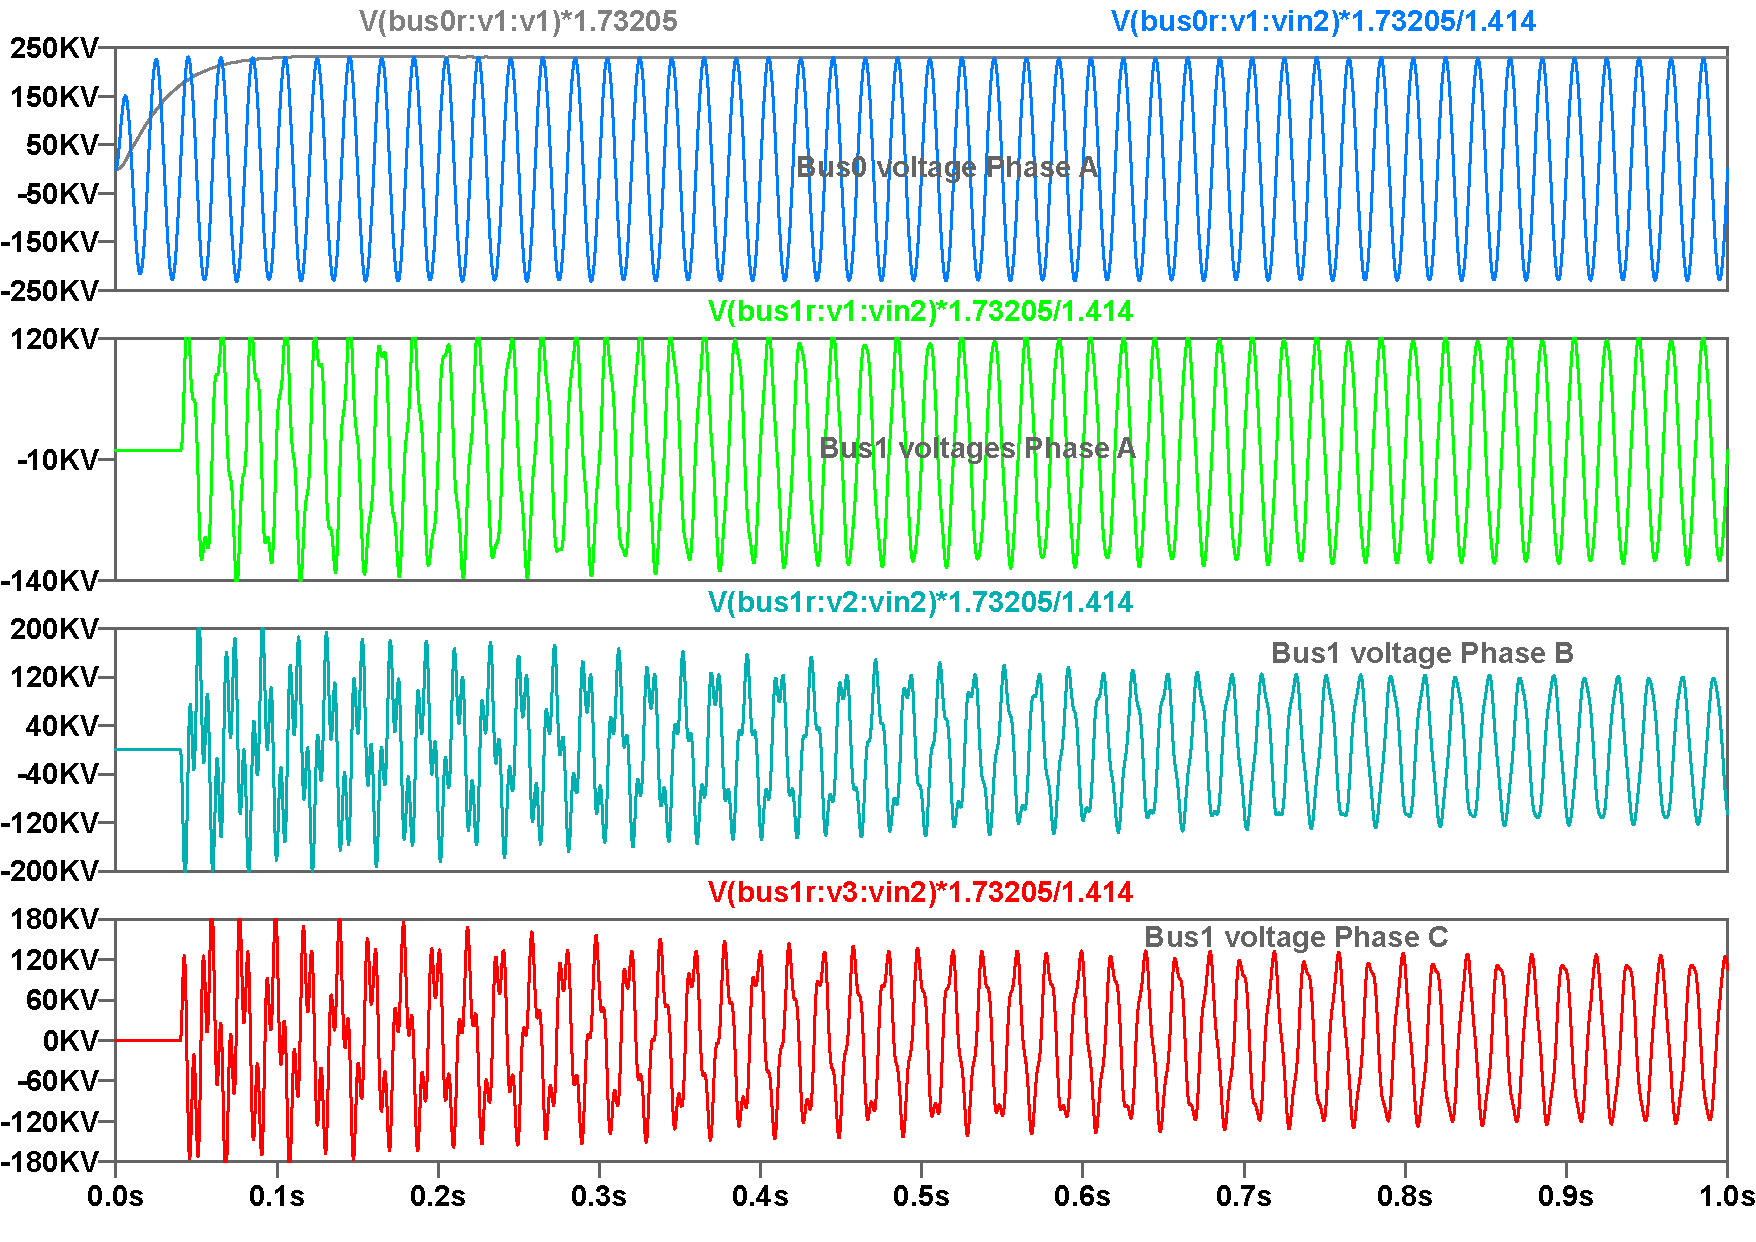
\includegraphics[width=0.90\textwidth]{figures/06_Switching_on_networks/Switching_on_networks_Bus0_Bus1_voltages-case5}
	\caption{Switching on networks voltages - case5}
	\label{fig:figure620}
\end{figure}

\begin{figure}[H]
	\centering
	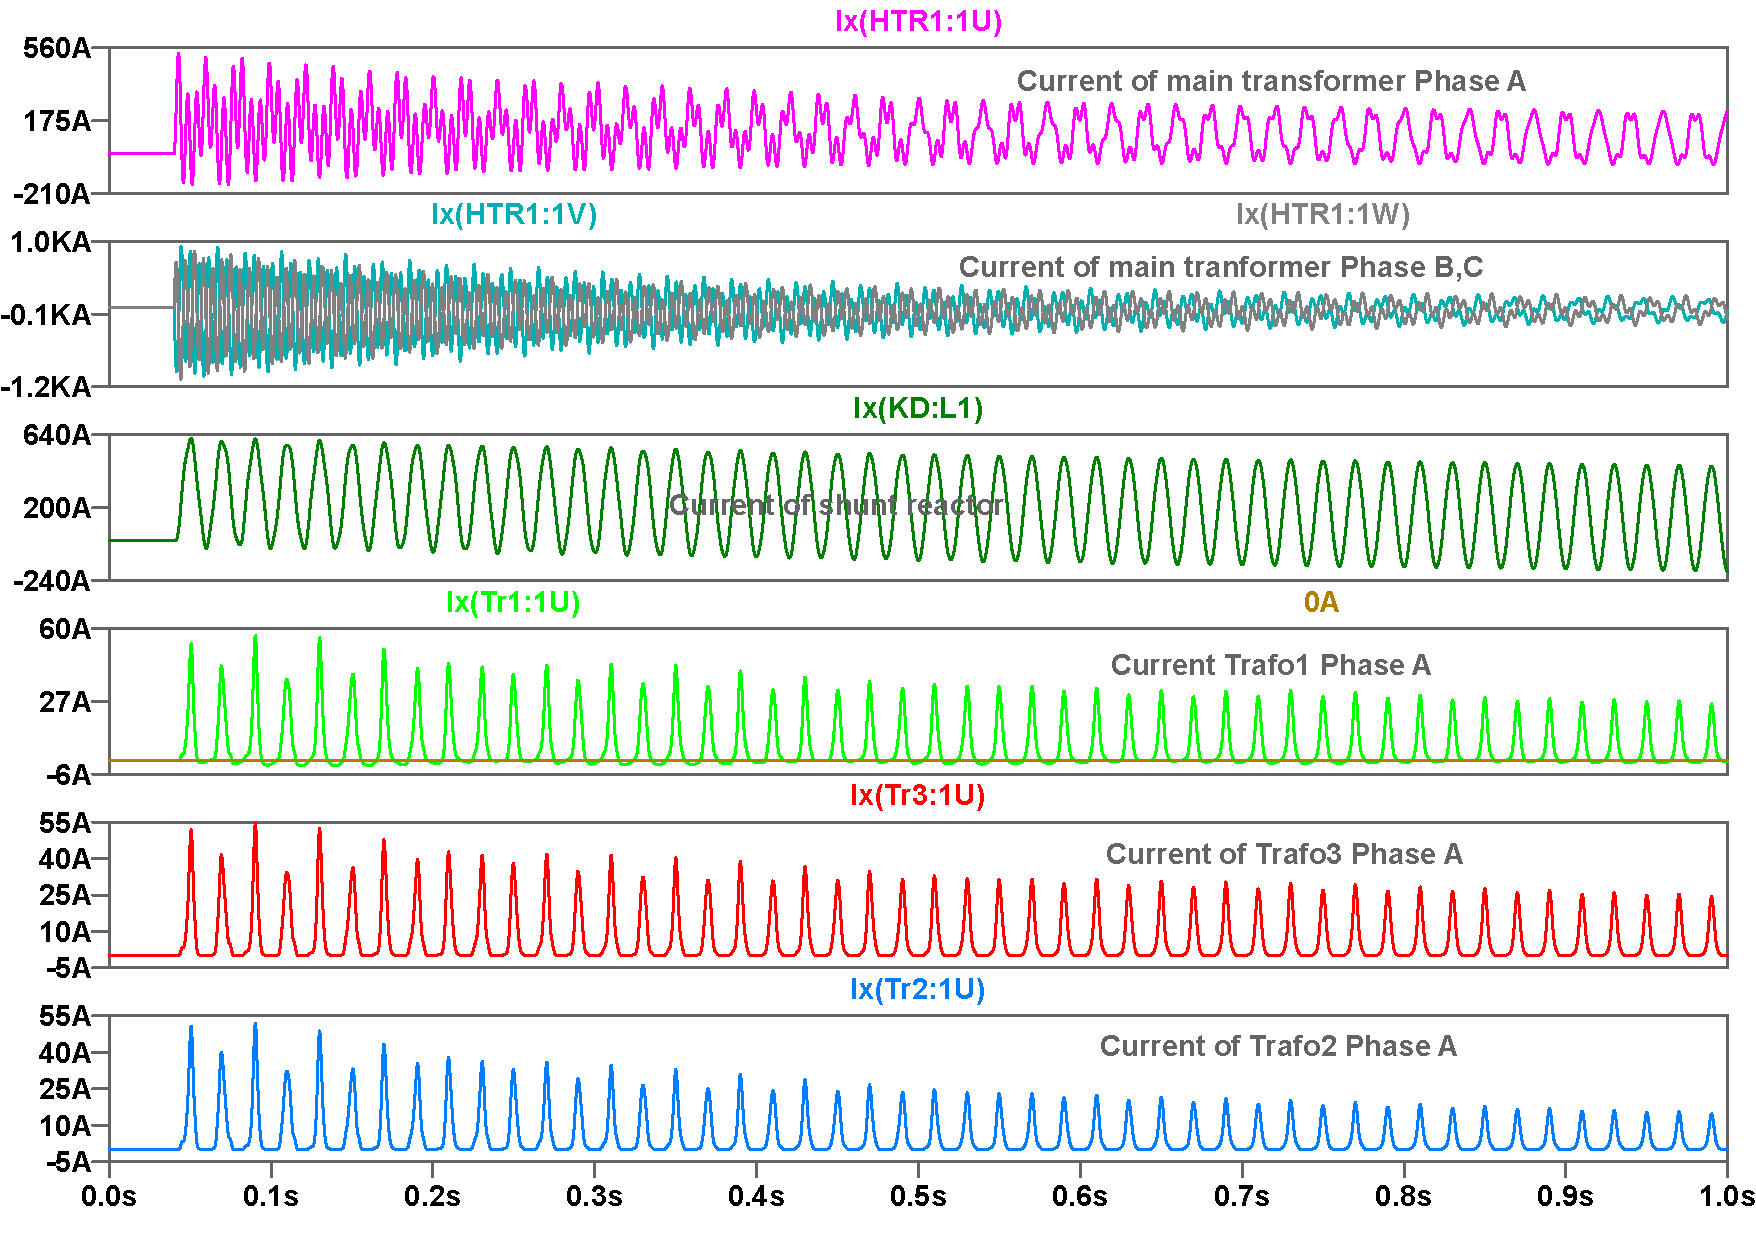
\includegraphics[width=0.90\textwidth]{figures/06_Switching_on_networks/Switching_on_networks_currents-case5}
	\caption{Switching on networks currents - case5}
	\label{fig:figure621}
\end{figure}

\begin{figure}[H]
	\centering
	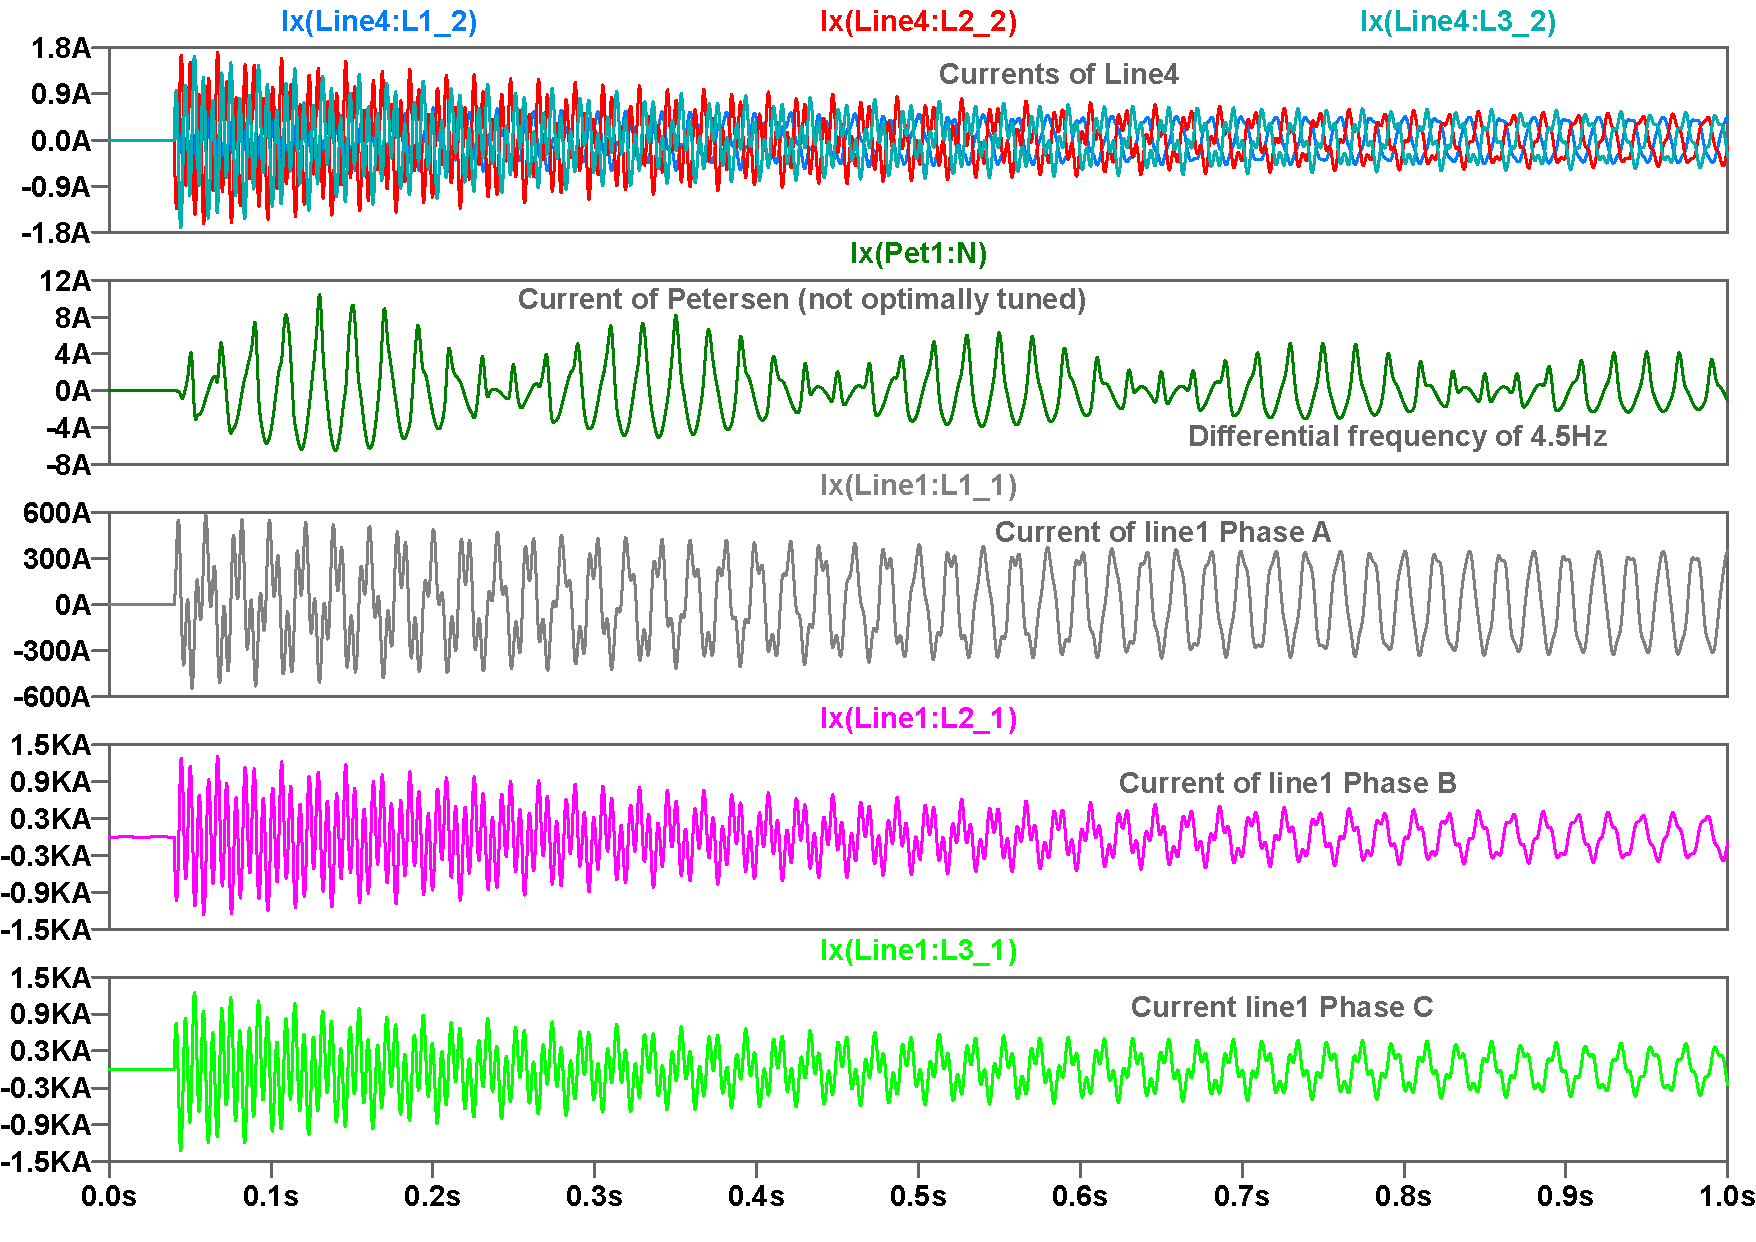
\includegraphics[width=0.90\textwidth]{figures/06_Switching_on_networks/Switching_on_networks_currents_Line1_Line4-case5}
	\caption{Switching on networks currents line1, line4 - case5}
	\label{fig:figure622}
\end{figure}

\begin{figure}[H]
	\centering
	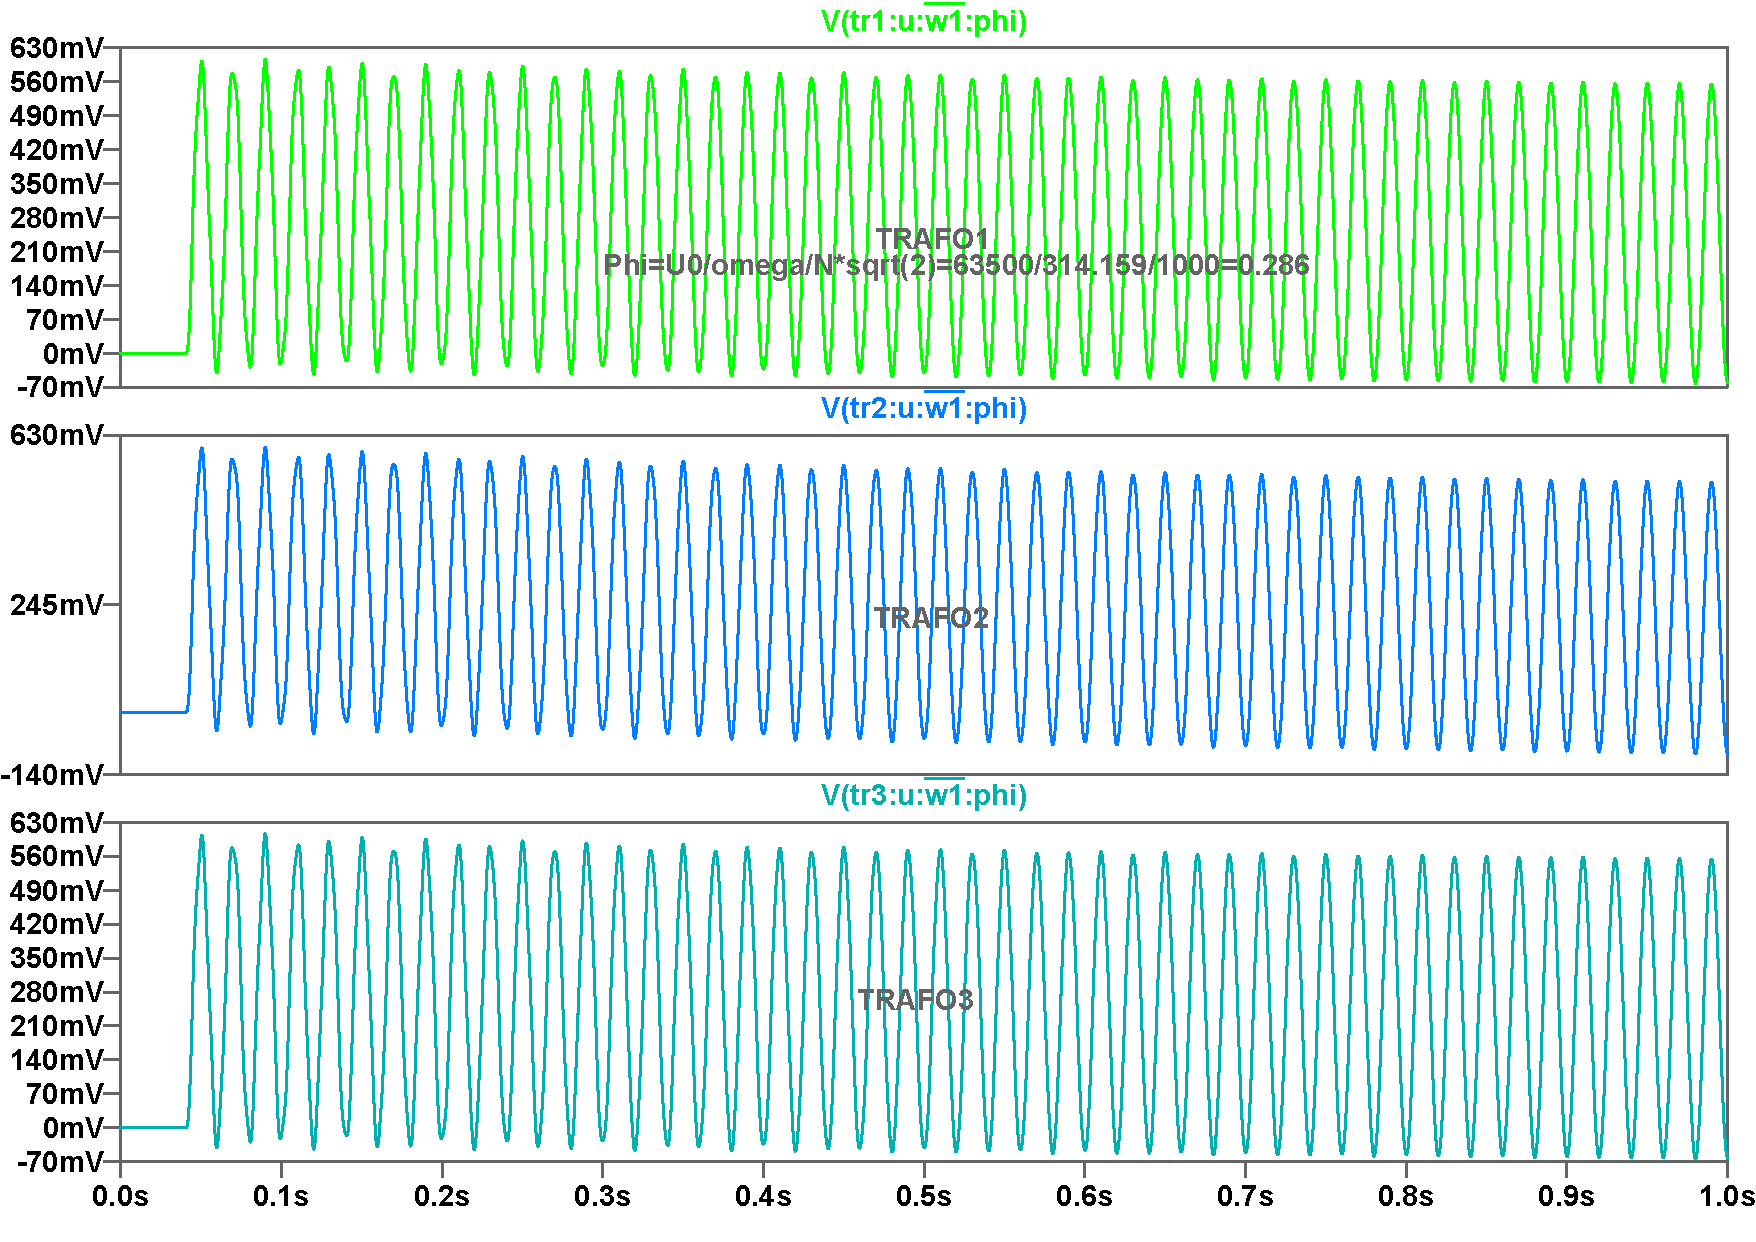
\includegraphics[width=0.90\textwidth]{figures/06_Switching_on_networks/Switching_on_networks_phi-case5}
	\caption{Switching on networks fluxes - case5}
	\label{fig:figure623}
\end{figure}

\begin{figure}[H]
	\centering
	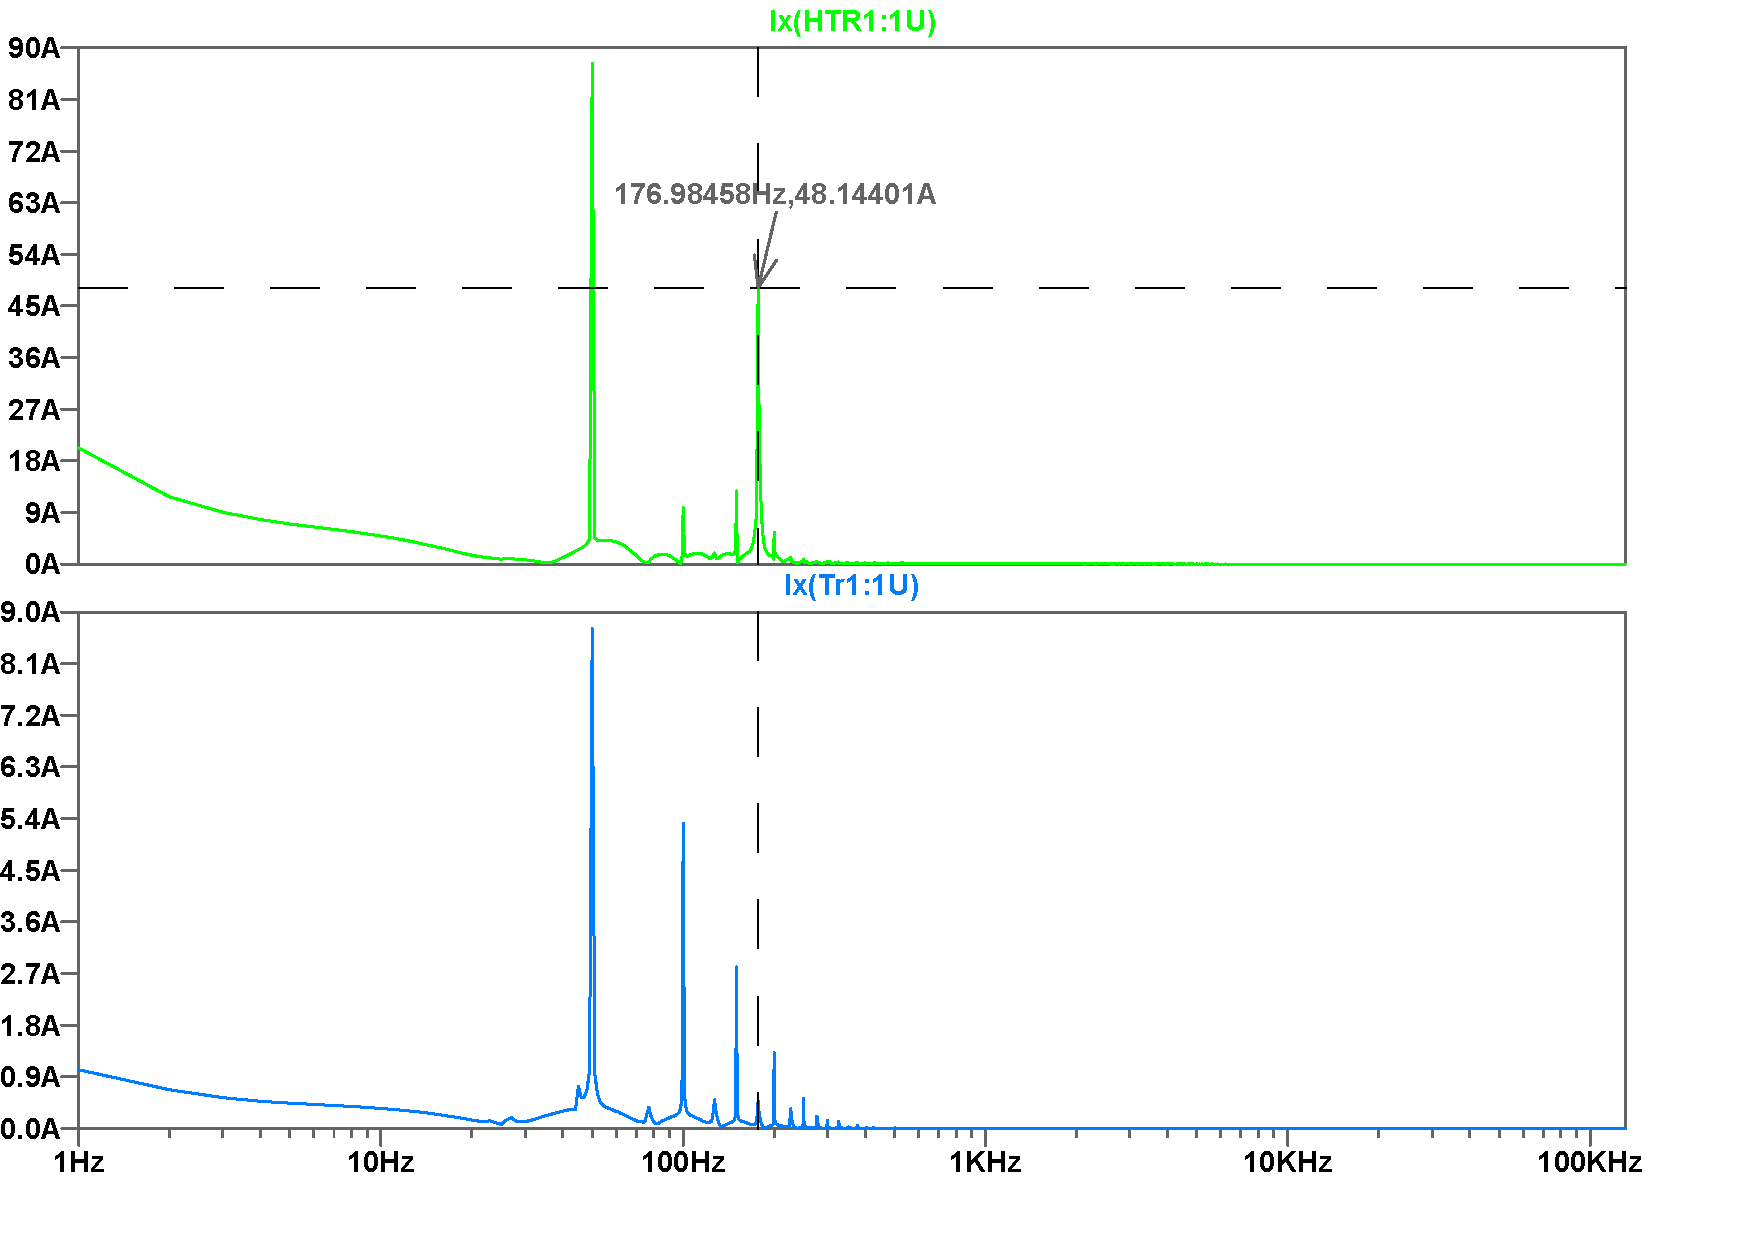
\includegraphics[width=0.90\textwidth]{figures/06_Switching_on_networks/Switching_on_networks_FFT_Transformer-case5}
	\caption{Switching on networks FFT - case5}
	\label{fig:figure624}
\end{figure}


% Measurement values table for the Power System Simulation book.
% Required packages are already loaded by the central preamble:
% booktabs, tabularx, array, siunitx, xcolor.

\begin{table}[htbp]
  \centering
  \caption{Signal ranges for Case 5. All values are peak values, bus values are multiplied by 1.73/1.414}
  \label{tab:measurement-values-case5}
  \small
  \setlength{\tabcolsep}{3.5pt}
  \renewcommand{\arraystretch}{1.18}
  \begin{tabularx}{\textwidth}{@{}
      >{\raggedright\arraybackslash}p{0.055\textwidth}
      >{\raggedright\arraybackslash}p{0.085\textwidth}
      >{\raggedright\arraybackslash}p{0.095\textwidth}
      >{\raggedright\arraybackslash}p{0.105\textwidth}
      >{\raggedright\arraybackslash}p{0.075\textwidth}
      >{\raggedright\arraybackslash}p{0.075\textwidth}
      Y@{}}
    \toprule
    \textbf{Meas.} &
    \textbf{Grid element} &
    \textbf{Phase} &
    \textbf{Voltage level} &
    \textbf{Min.} &
    \textbf{Max.} &
    \textbf{Notes} \\
    \midrule
    $V$ & Bus0  & Ph A       & \SI{220}{\kilo\volt} & \SI{-229}{\kilo\volt} & \SI{229}{\kilo\volt} & -- \\
    $V$ & Bus1  & Ph A,    & \SI{110}{\kilo\volt} & \SI{-140}{\kilo\volt} & \SI{120}{\kilo\volt} & -- \\
    $V$ & Bus1  & Ph B,C     & \SI{110}{\kilo\volt} & \SI{-180}{\kilo\volt} & \SI{180}{\kilo\volt} & -- \\
    $I$ & HTr1  & Ph A       & \SI{220}{\kilo\volt} & \SI{-160}{\ampere} & \SI{530}{\ampere} & -- \\
    $I$ & HTr1  & Ph B, C    & \SI{220}{\kilo\volt} & \SI{-1}{\kilo\ampere} & \SI{1}{\kilo\ampere} & -- \\
    $I$ & KD1   & Ph A       & \SI{110}{\kilo\volt} & \SI{0}{\ampere} & \SI{620}{\ampere} & Steady state: \SI{300}{\ampere} \\
    $I$ & Tr1   & Ph A       & \SI{110}{\kilo\volt} & \SI{0}{\ampere} & \SI{54}{\ampere} &  Fluctuating \\
    $I$ & Tr2   & Ph A       & \SI{110}{\kilo\volt} & \SI{0}{\ampere} & \SI{52}{\ampere} &  Fluctuating \\
    $I$ & Tr3   & Ph A      & \SI{110}{\kilo\volt} & \SI{0}{\ampere} & \SI{52}{\ampere} &  Fluctuating \\
    $I$ & Line4 & Ph A & \SI{110}{\kilo\volt} & \SI{-1.6}{\ampere} & \SI{1.6}{\ampere} & Small capacitive inrush current  \\
    $I$ & Line1 & Ph A & \SI{110}{\kilo\volt} & \SI{-530}{\ampere} & \SI{600}{\ampere} & High capacitive inrush current due to cable \\
    $I$ & Line1 & Ph B, C & \SI{110}{\kilo\volt} & \SI{-1.3}{\kilo\ampere} & \SI{1.3}{\kilo\ampere} & High capacitive inrush current due to cable \\
    $I$ & Pet1 & Ph N & \SI{110}{\kilo\volt} & \SI{-6}{\ampere} & \SI{10}{\ampere} & Fluctuating, Longtime value very small \\
    $V$ & Pet1 & Ph N & \SI{110}{\kilo\volt} & \SI{-800}{\volt} & \SI{600}{\volt} & Fluctuating, Longtime value very small \\
    $\Phi$ & Tr1 & Ph A, B, C   & \SI{110}{\kilo\volt} & \SI{0}{\weber} & \SI{0.60}{\weber} & Nominal flux: 
    \SI{0.288}{\weber} \\
    FFT & HTr1  & Ph C       & \SI{220}{\kilo\volt} & \SI{50}{\hertz} & \SI{178}{\hertz} & mostly \SI{50}{\hertz} and \SI{178}{\hertz} \\
    FFT & Tr2   & Ph A       & \SI{110}{\kilo\volt} & \SI{50}{\hertz} & \SI{250}{\hertz} & \SI{50}{\hertz}, \SI{100}{\hertz}, \SI{150}{\hertz}, \SI{200}{\hertz}, and \SI{250}{\hertz} \\
    \bottomrule
  \end{tabularx}
\end{table}




\section{Case 6: Energization with Load}
\label{sec:network-energization-with-load}

Set \texttt{lf=0.5}. The connected load strongly dampens the overvoltages caused
by the high-frequency capacitive charging currents, and these oscillations
decay rapidly. Transformer inrush currents remain present because they are caused
by the transient core flux. Among the direct-switching cases considered so
far, this case produces the smallest overvoltages.

The current on the 10.6 kV side of the load is 360 A,
which is approximately 36 A on the 110 kV side. The currents on the 110 kV side are
a mixture of inrush currents and load currents.
It is often claimed in the literature that the load current
reduces the inrush of the magnetizing current.
This is not really the case. This can be easily demonstrated by simultaneously simulating three identical transformers:
a) Set m=1 for Transformer 1 and apply a load to it. This measures the load current on the primary side.
b) Set m = 9 for Transformer 2 and set the load to zero.
c) For Transformer 3, set m=9 and connect the same load. The resulting currents can then be compared.
Now you can see that when adding the primary currents I(Transformer 1) + I(Transformer 2), the resulting current is approximately equal to I(Transformer 3). Any reduction in inrush current is very small in this example. The transformer inrush is simply “hidden” in the total current but is always present. See ltspice file \texttt{Hidden\_inrush.asc}
 
\begin{figure}[H]
	\centering
	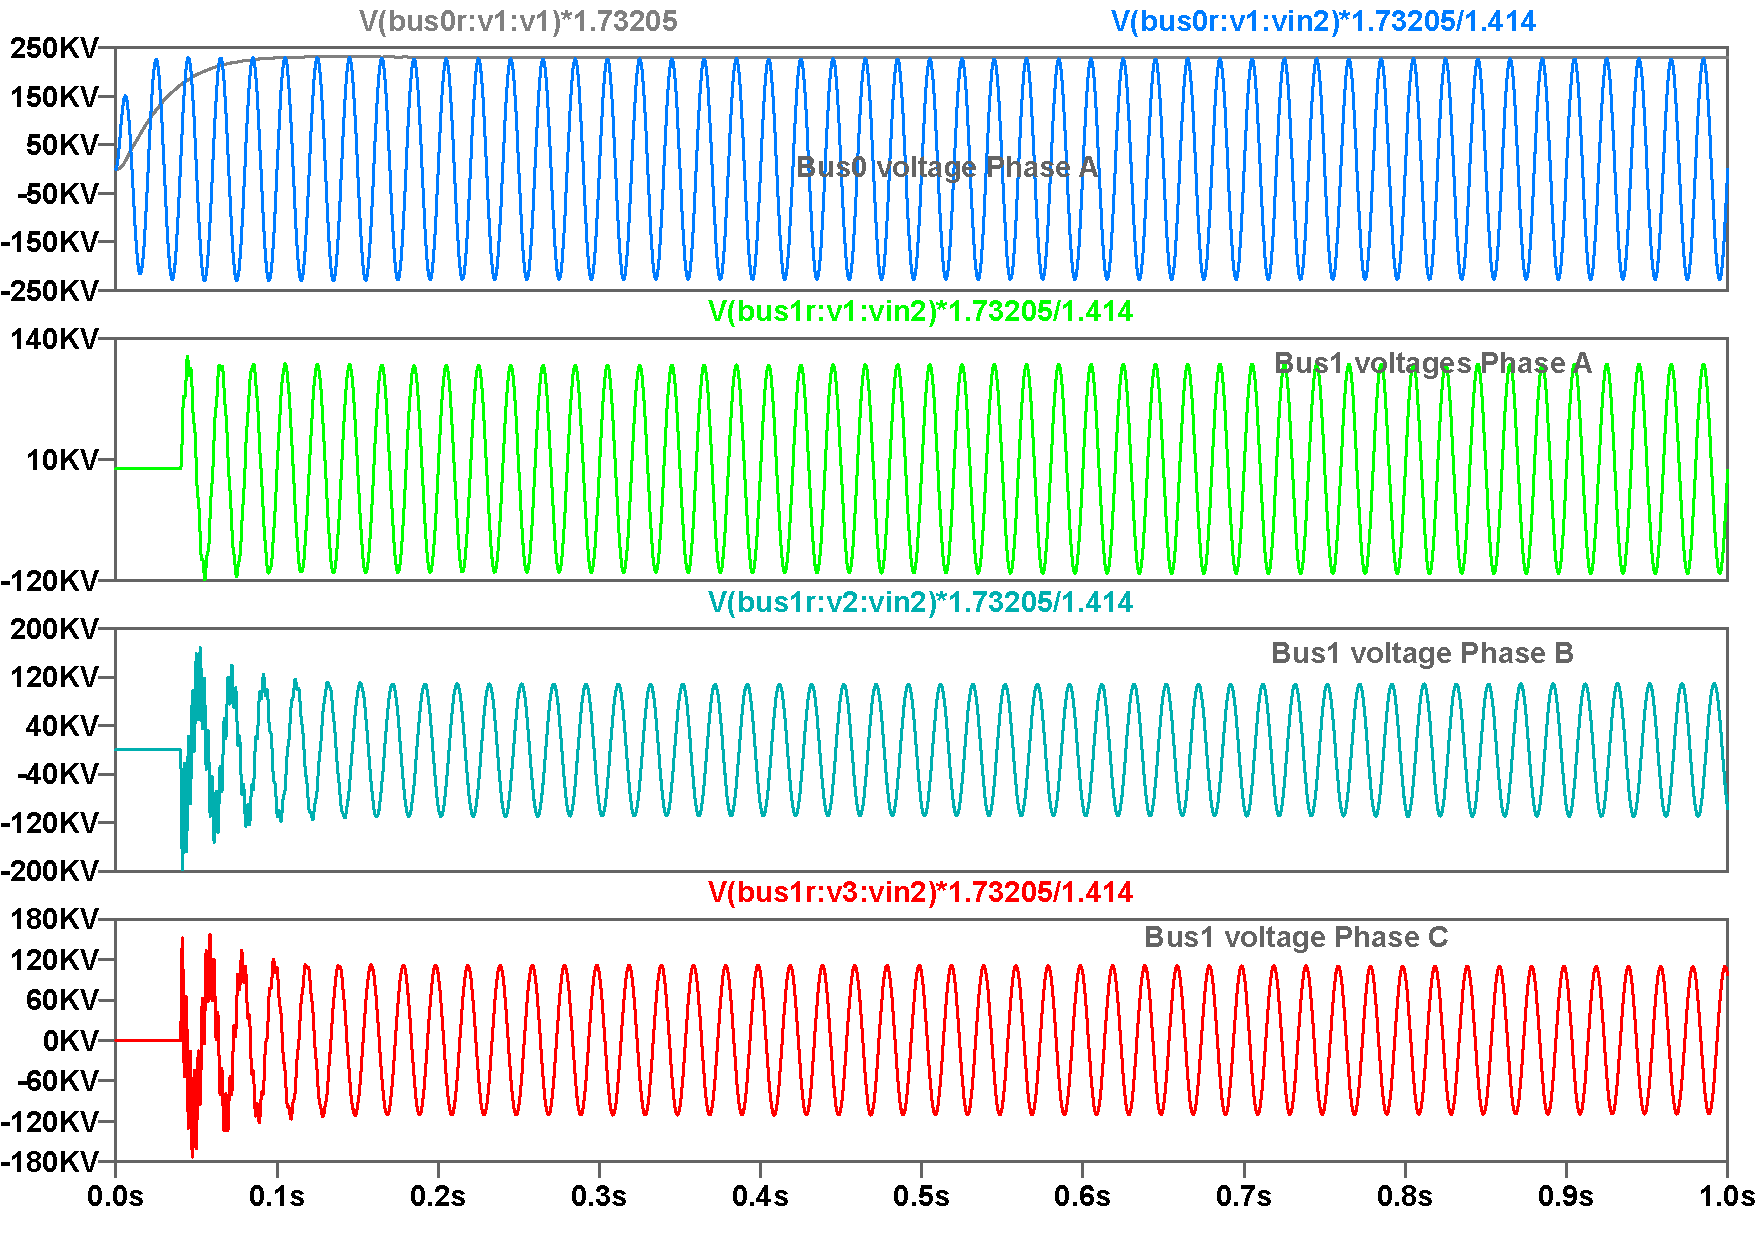
\includegraphics[width=0.90\textwidth]{figures/06_Switching_on_networks/Switching_on_networks_Bus0_Bus1_voltages-case6}
	\caption{Switching on networks voltages - case6}
	\label{fig:figure625}
\end{figure}

\begin{figure}[H]
	\centering
	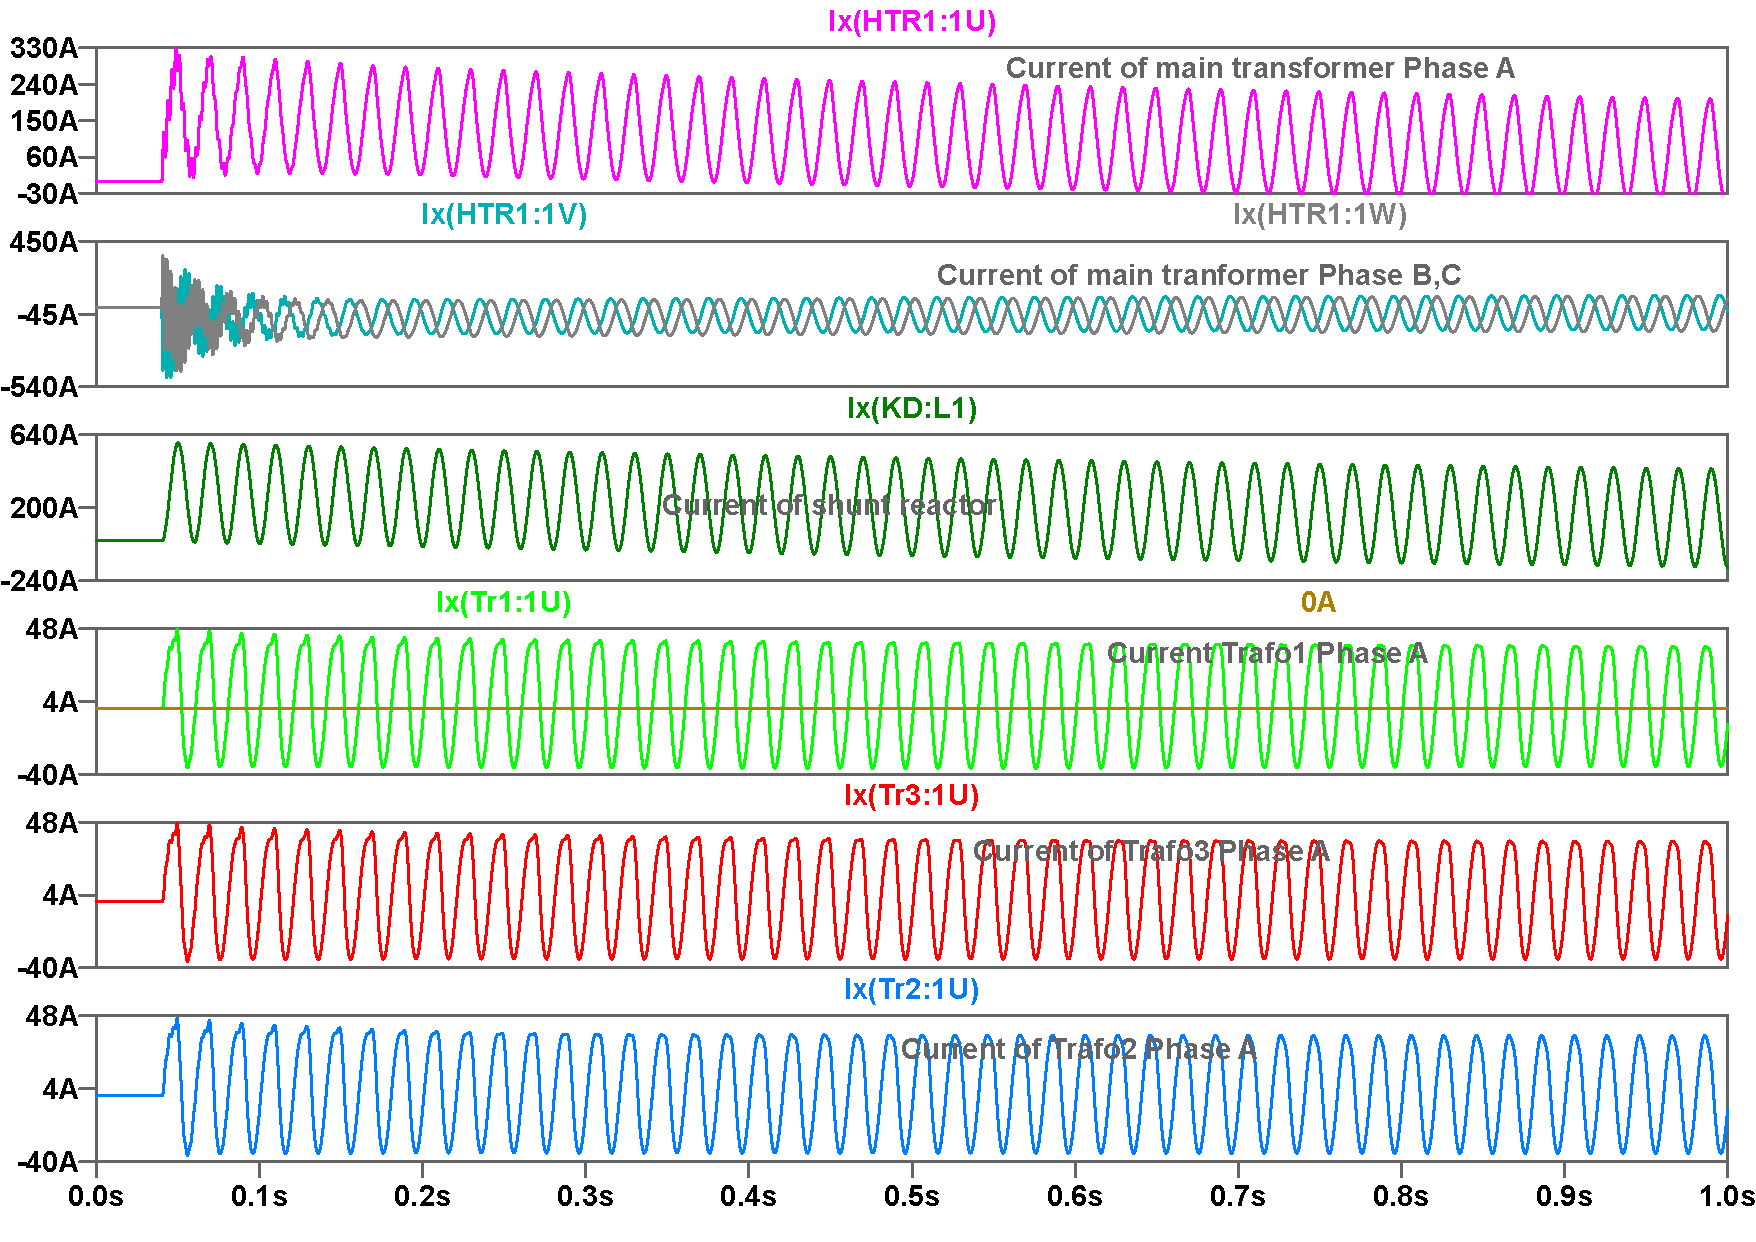
\includegraphics[width=0.90\textwidth]{figures/06_Switching_on_networks/Switching_on_networks_currents-case6}
	\caption{Switching on networks currents - case6}
	\label{fig:figure626}
\end{figure}

\begin{figure}[H]
	\centering
	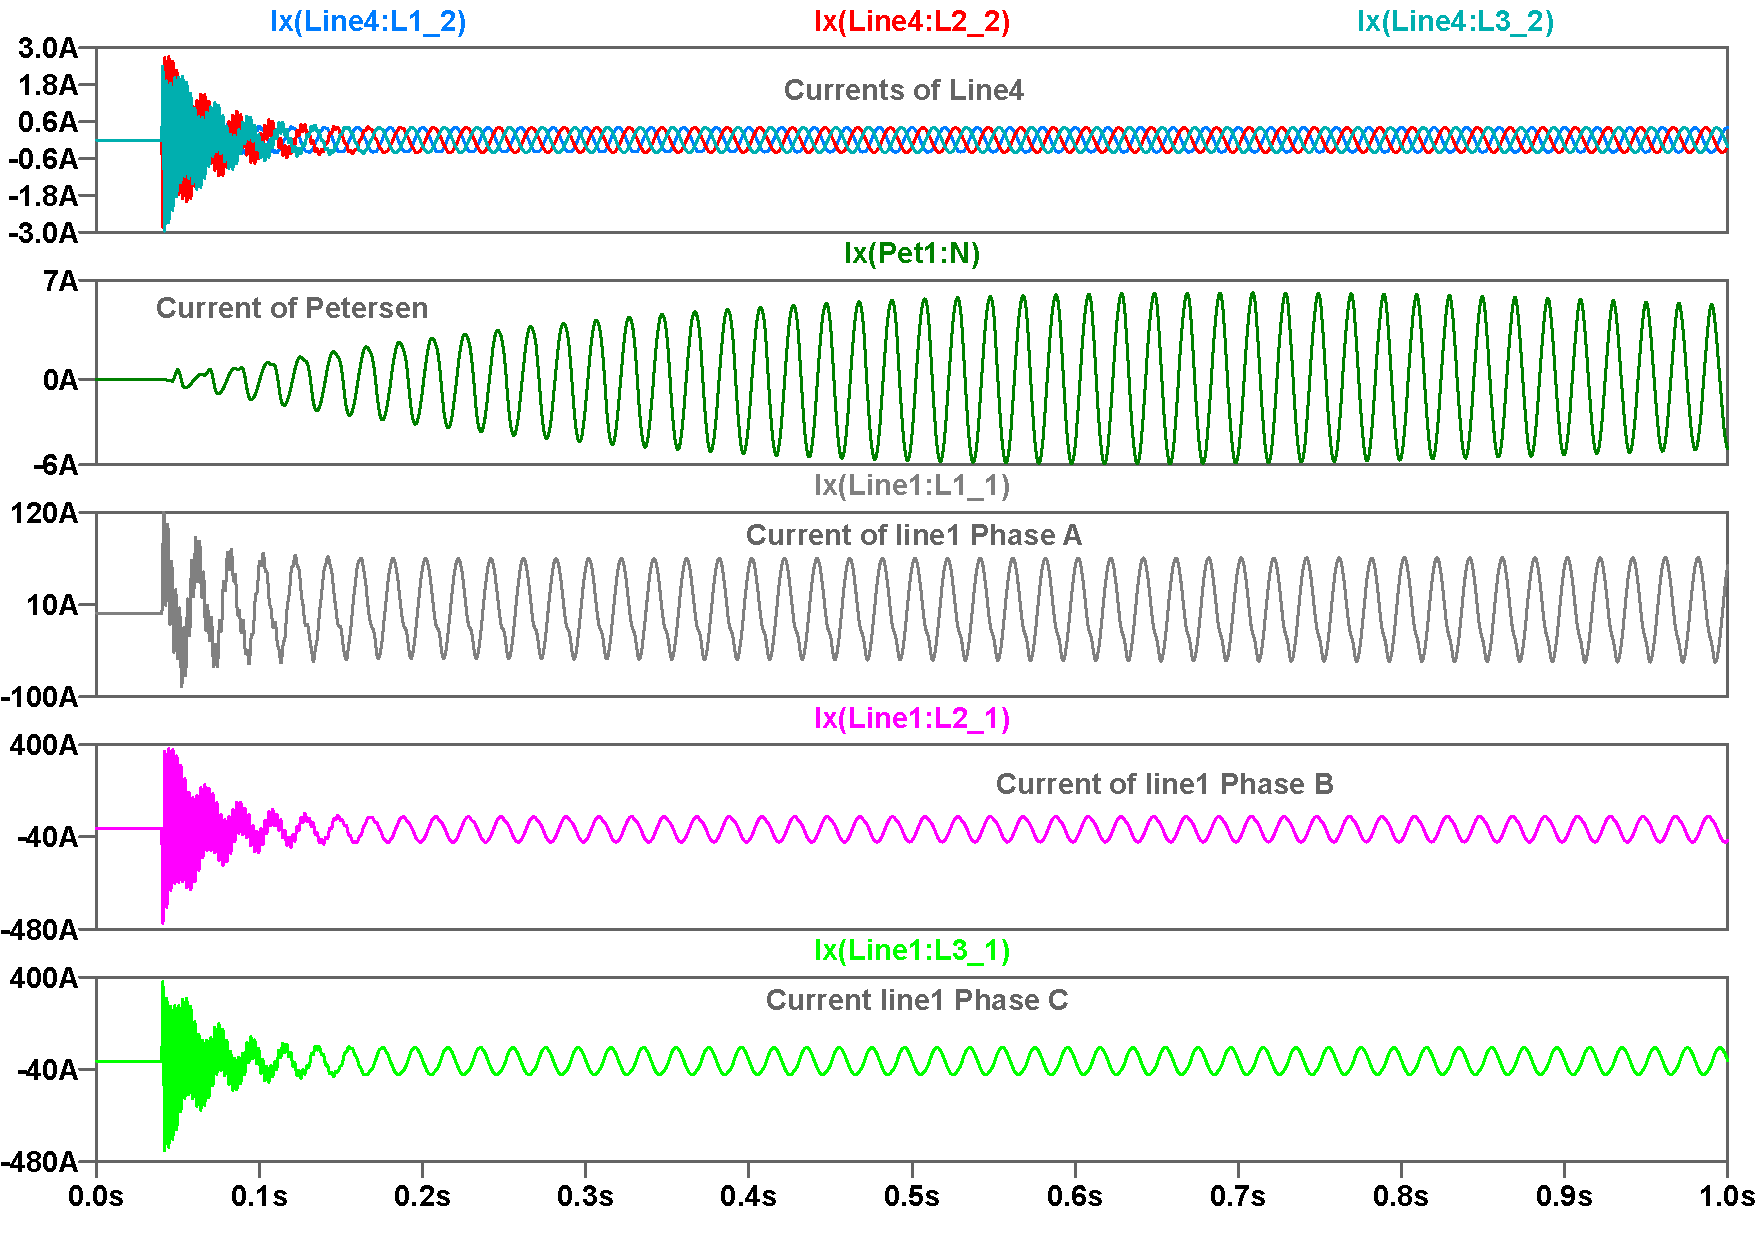
\includegraphics[width=0.90\textwidth]{figures/06_Switching_on_networks/Switching_on_networks_currents_Line1_Line4-case6}
	\caption{Switching on networks currents line1, line4 - case6}
	\label{fig:figure627}
\end{figure}

\begin{figure}[H]
	\centering
	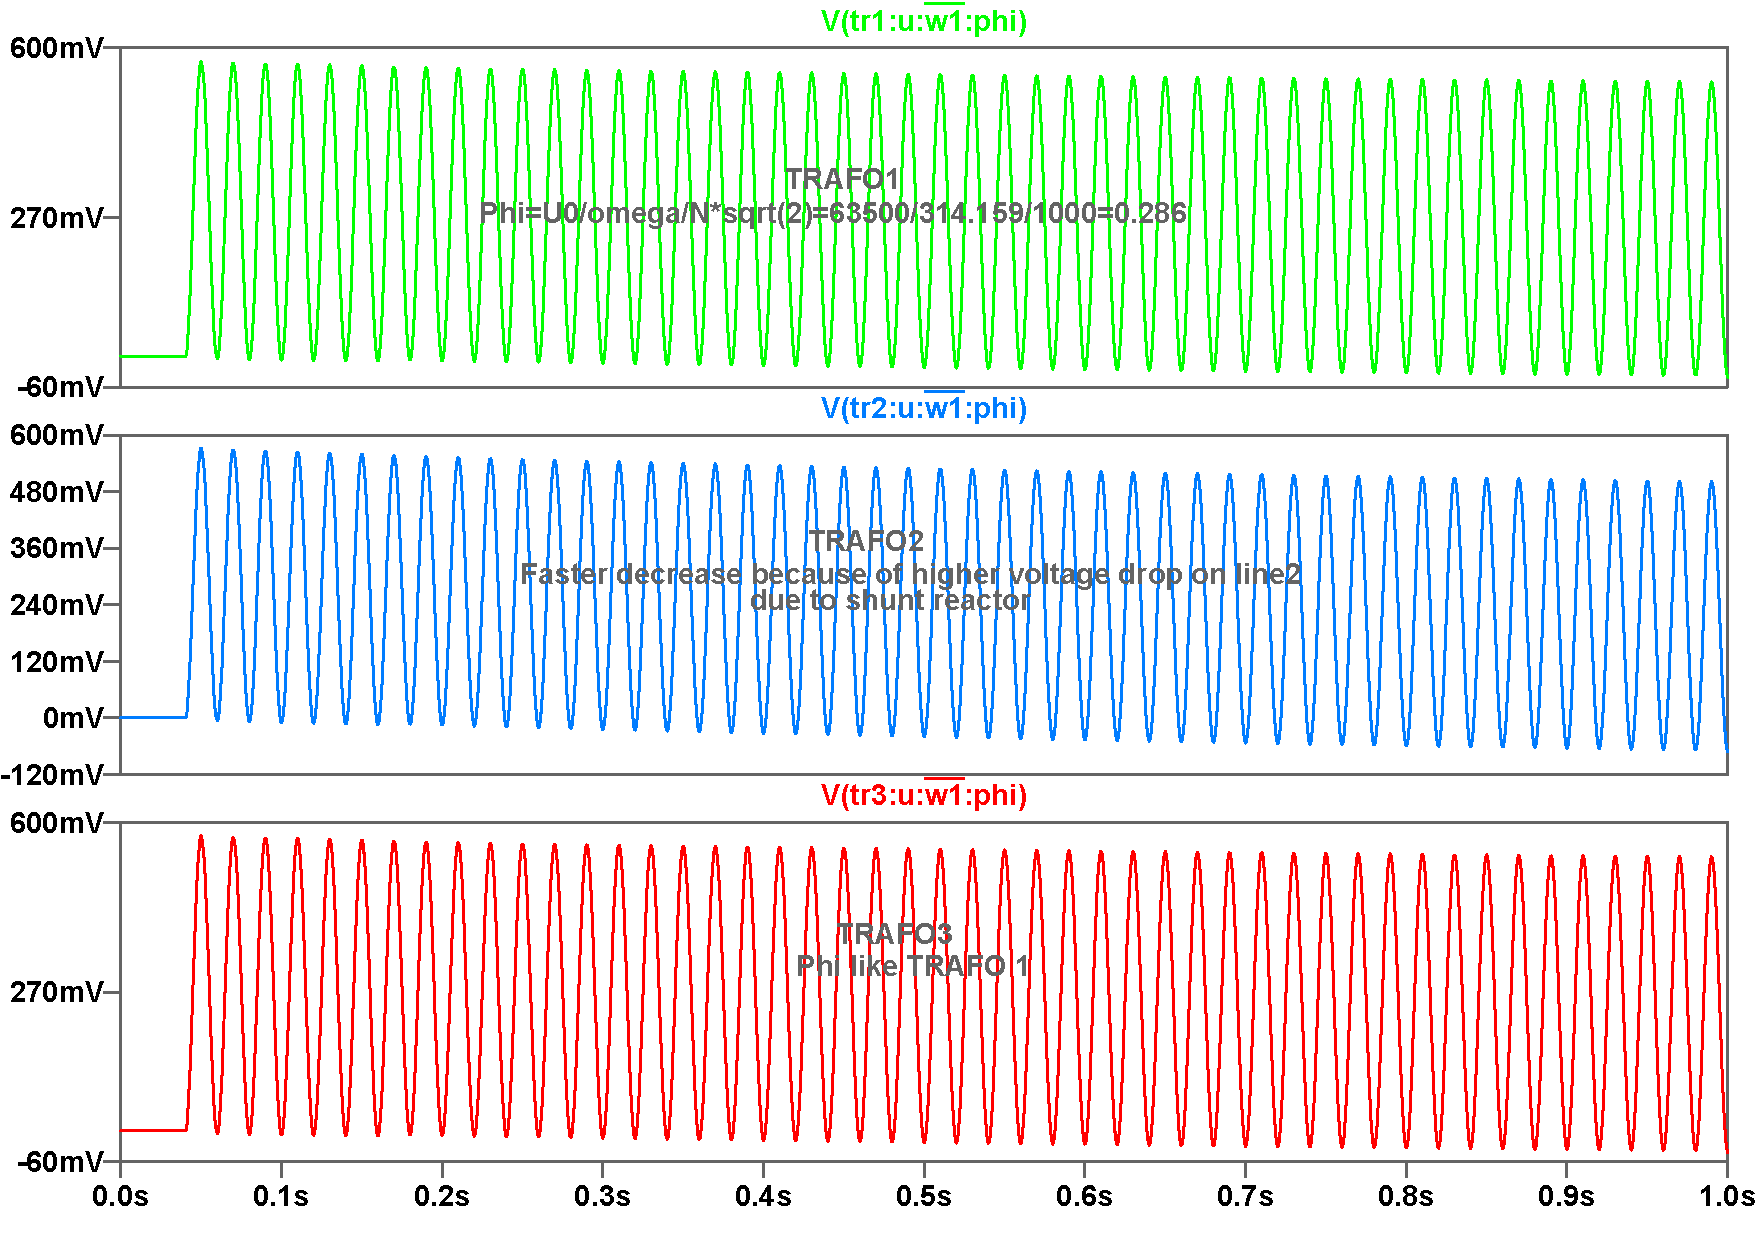
\includegraphics[width=0.90\textwidth]{figures/06_Switching_on_networks/Switching_on_networks_phi-case6}
	\caption{Switching on networks fluxes - case6}
	\label{fig:figure628}
\end{figure}


% Measurement values table for the Power System Simulation book.
% Required packages are already loaded by the central preamble:
% booktabs, tabularx, array, siunitx, xcolor.

\begin{table}[htbp]
  \centering
  \caption{Signal ranges for Case 6. All values are peak values, bus values are multiplied by 1.73/1.414}
  \label{tab:measurement-values-case6}
  \small
  \setlength{\tabcolsep}{3.5pt}
  \renewcommand{\arraystretch}{1.18}
  \begin{tabularx}{\textwidth}{@{}
      >{\raggedright\arraybackslash}p{0.055\textwidth}
      >{\raggedright\arraybackslash}p{0.085\textwidth}
      >{\raggedright\arraybackslash}p{0.095\textwidth}
      >{\raggedright\arraybackslash}p{0.105\textwidth}
      >{\raggedright\arraybackslash}p{0.075\textwidth}
      >{\raggedright\arraybackslash}p{0.075\textwidth}
      Y@{}}
    \toprule
    \textbf{Meas.} &
    \textbf{Grid element} &
    \textbf{Phase} &
    \textbf{Voltage level} &
    \textbf{Min.} &
    \textbf{Max.} &
    \textbf{Notes} \\
    \midrule
    $V$ & Bus0  & Ph A       & \SI{220}{\kilo\volt} & \SI{-229}{\kilo\volt} & \SI{229}{\kilo\volt} & -- \\
    $V$ & Bus1  & Ph A,    & \SI{110}{\kilo\volt} & \SI{-120}{\kilo\volt} & \SI{120}{\kilo\volt} & -- \\
    $V$ & Bus1  & Ph B,C     & \SI{110}{\kilo\volt} & \SI{-170}{\kilo\volt} & \SI{160}{\kilo\volt} & -- \\
    $I$ & HTr1  & Ph A       & \SI{220}{\kilo\volt} & \SI{0}{\ampere} & \SI{330}{\ampere} & -- \\
    $I$ & HTr1  & Ph B, C    & \SI{220}{\kilo\volt} & \SI{-480}{\ampere} & \SI{360}{\ampere} & -- \\
    $I$ & KD1   & Ph A       & \SI{110}{\kilo\volt} & \SI{0}{\ampere} & \SI{590}{\ampere} & Steady state: \SI{300}{\ampere} \\
    $I$ & Tr1   & Ph A       & \SI{110}{\kilo\volt} & \SI{-36}{\ampere} & \SI{54}{\ampere} & under load \\
    $I$ & Tr2   & Ph A       & \SI{110}{\kilo\volt} & \SI{-36}{\ampere} & \SI{50}{\ampere} & under load \\
    $I$ & Tr3   & Ph A      & \SI{110}{\kilo\volt} & \SI{-36}{\ampere} & \SI{47}{\ampere} & under load \\
    $I$ & Line4 & Ph A & \SI{110}{\kilo\volt} & \SI{-3}{\ampere} & \SI{2.5}{\ampere} & Small capacitive inrush current  \\
    $I$ & Line1 & Ph A & \SI{110}{\kilo\volt} & \SI{-90}{\ampere} & \SI{120}{\ampere} & High capacitive inrush current due to cable \\
    $I$ & Line1 & Ph B, C & \SI{110}{\kilo\volt} & \SI{-480}{\ampere} & \SI{380}{\ampere} & High capacitive inrush current due to cable \\
    $I$ & Pet1 & Ph N & \SI{110}{\kilo\volt} & \SI{-6}{\ampere} & \SI{6}{\ampere} & Longtime value very small \\
    $V$ & Pet1 & Ph N & \SI{110}{\kilo\volt} & \SI{-1.5}{\kilo\volt} & \SI{1.5}{\kilo\volt} & Longtime value very small \\
    $\Phi$ & Tr1 & Ph A, B, C   & \SI{110}{\kilo\volt} & \SI{0}{\weber} & \SI{0.575}{\weber} & Nominal flux: 
    \SI{0.288}{\weber} \\
    \bottomrule
  \end{tabularx}
\end{table}

 
 
  

\section{Case 7: Skin-Effect Model}
\label{sec:network-skin-effect}

Set \texttt{skin=1}. To apply the skin effect in a rough way, we make the simplified assumption that up to 40 ms, only the 50 Hz component determines the resistance, and from 40 ms onward, only the higher frequency of 400 Hz determines the resistance. (Normally, the 50 Hz and 400 Hz components contribute equally). This allows us to roughly determine the influence of the higher frequency. We see that the additional damping is present but small. Even smaller when split between 50 Hz and 400 Hz. 
The effect is expected to be more pronounced in smaller networks with higher
natural frequencies, particularly when individual lines are energized.

\begin{figure}[H]
	\centering
	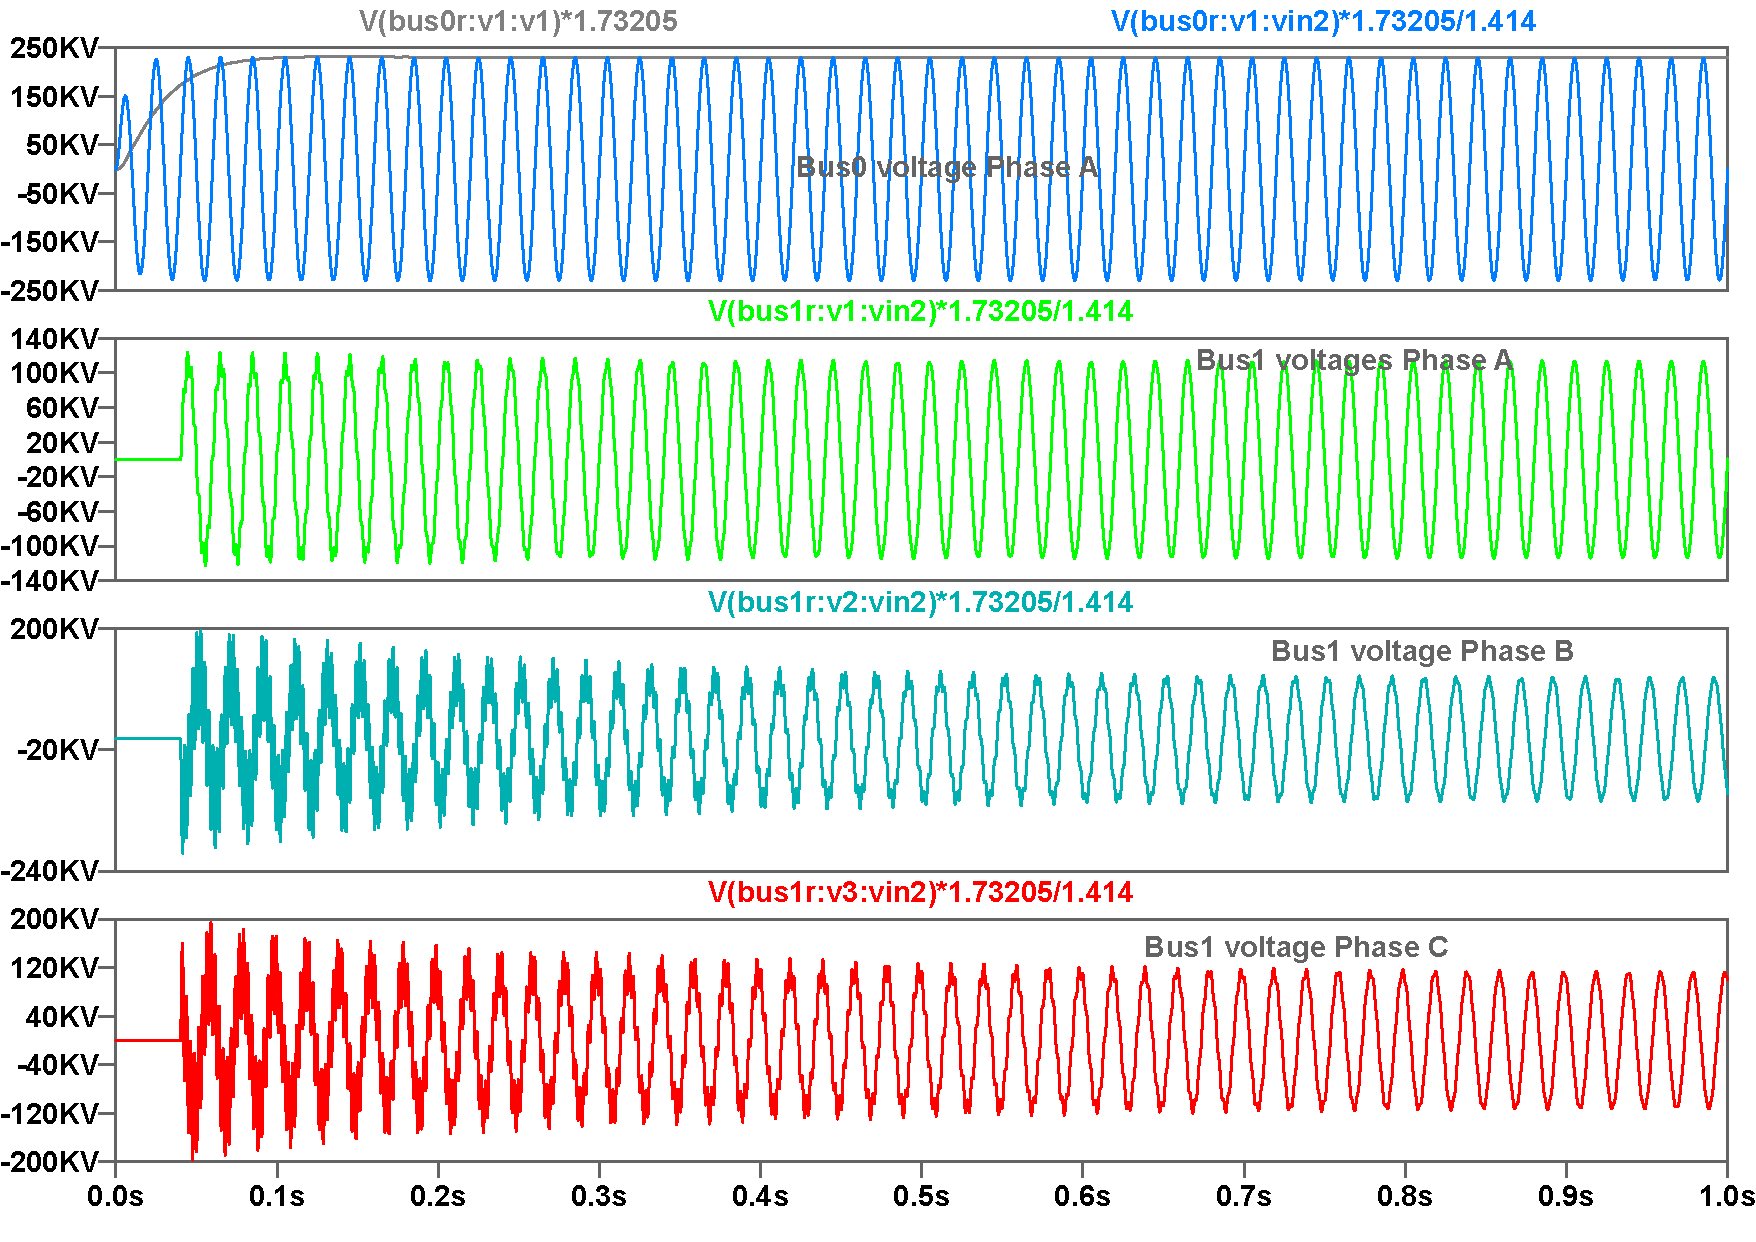
\includegraphics[width=0.90\textwidth]{figures/06_Switching_on_networks/Switching_on_networks_Bus0_Bus1_voltages-case7}
	\caption{Switching on networks voltages - case7}
	\label{fig:figure629}
\end{figure}


\section{Case 8: Energization from a Weak Network}

Set \texttt{weak=40} to increase the source impedance (This setting represents an additional transformer in series, as may occur during restoration after a blackout). The larger source
impedance limits the inrush current, although it may simultaneously increase
voltage sensitivity elsewhere in the network. Due to the higher voltage volatility, it is not advisable to use a shunt reactor in this circuit. It is better to regulate the voltage by tap-changing the transformer. Try it out and observe the steady-state value of the 110kV voltages. 
The 110kV steady state voltage is about 106kV with shunt reactor and 120kV without shunt reactor. There is a voltage drop of about 15kV !!
To see the difference in one plot add the line \texttt{.step param kd list 0 1} to the schematic !!

\begin{figure}[H]
	\centering
	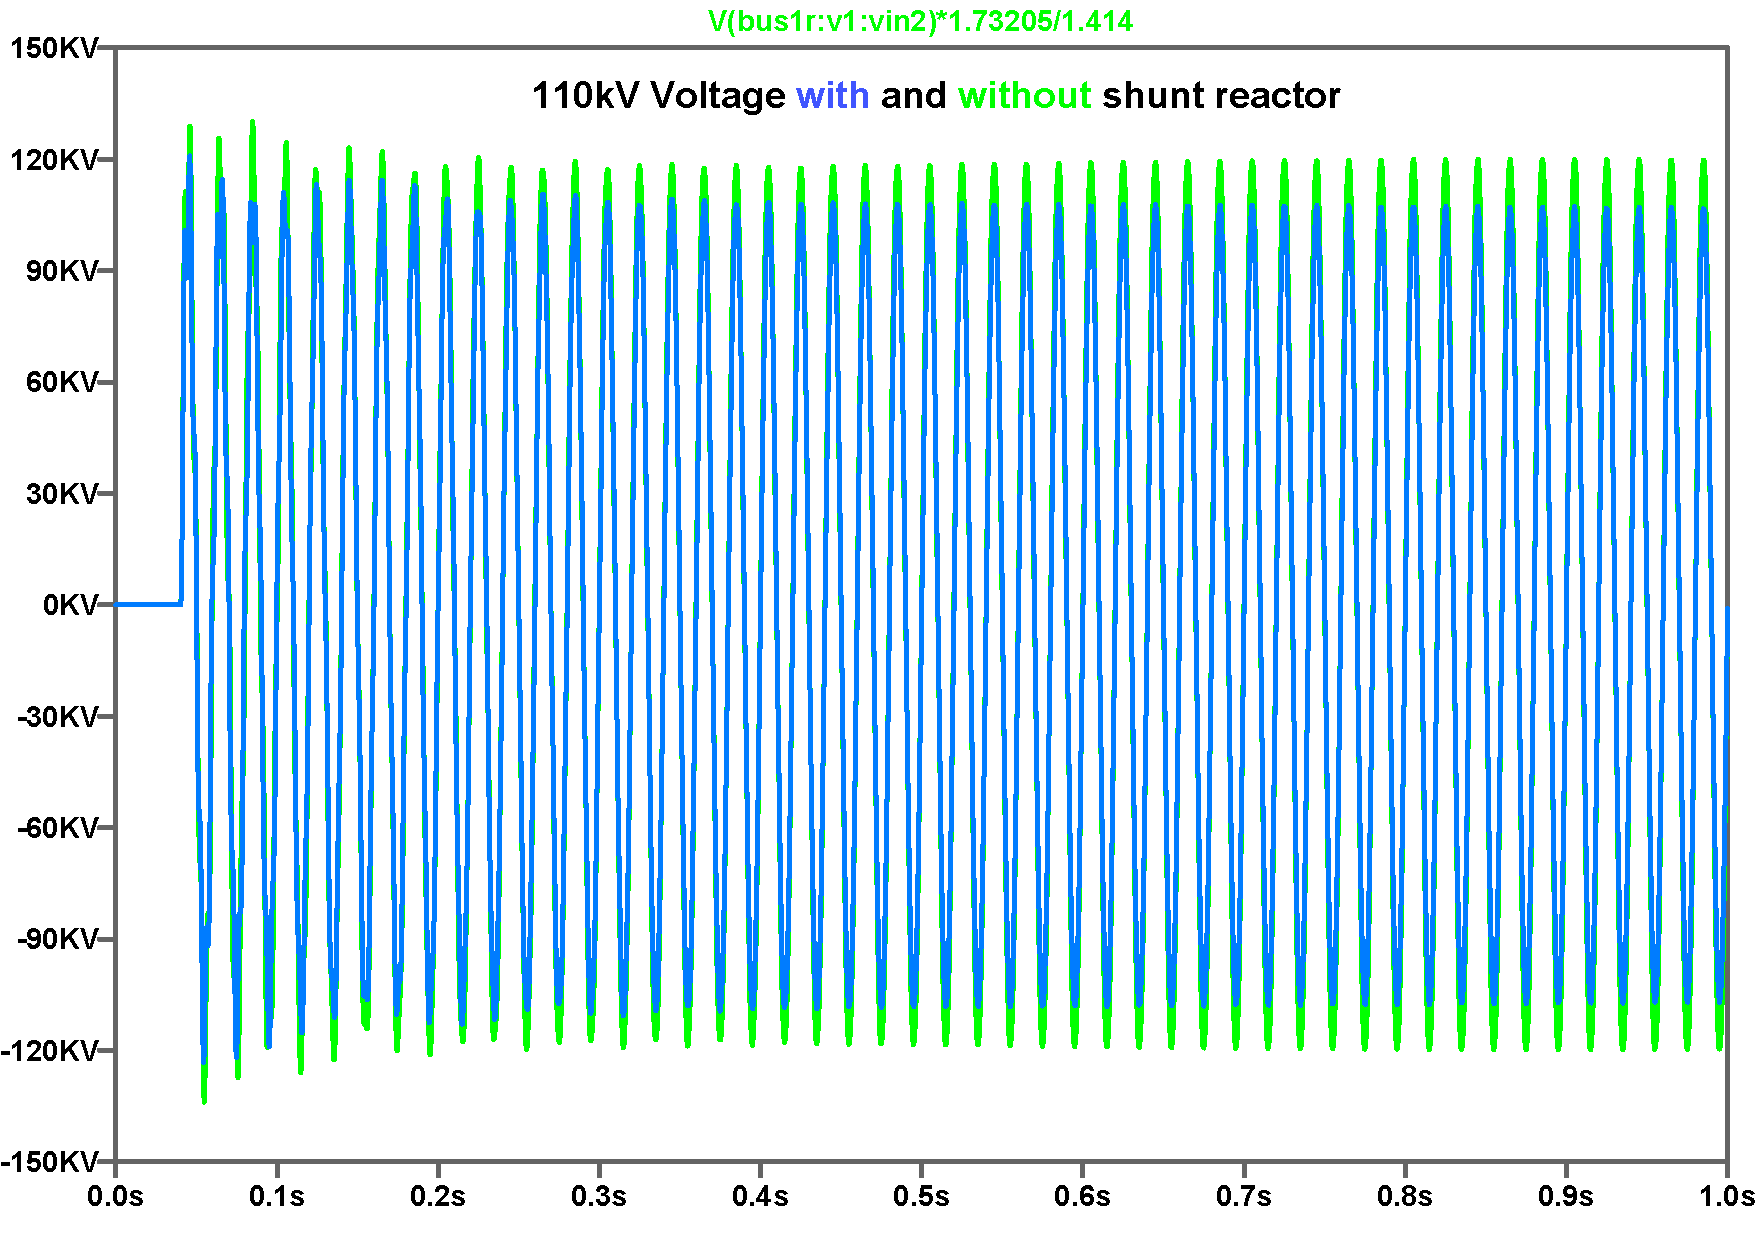
\includegraphics[width=0.90\textwidth]{figures/06_Switching_on_networks/Switching_on_networks_kd_on_off_case8}
	\caption{Switching on networks voltages - case8}
	\label{fig:figure630}
\end{figure}


\section{Case 9: Network Startup by a Voltage Ramp}
\label{sec:network-voltage-ramp}

The simulation file is
\texttt{Switching\_on\_networks\_Voltagetrip.asc}. Set the voltage-source parameter 
\texttt{tpwl} to \SI{400}{\milli\second} and remove the network
switch. Set the parameter ST to 10s to disable it. The source voltage then increases gradually from zero to its nominal
value within 400ms. NOTE: This is not really done in practice but in simulation
to keep the simulation time short.

This procedure produces practically no switching transients: there are no
significant over-voltages, high-frequency charging-current oscillations, or
transformer magnetizing inrush currents. It is therefore the preferred method
for energizing the complete network in this study. Loads should be connected
only after the voltage has reached its nominal level.
The currents of this network are only the charging currents of the lines
and the current of the shunt reactor. 
The magnetizing currents of the transformers 2 and 3 are below 1A.
The current of Transformer1 is a little bit higher due to the current needed by the Petersen.
The currents in all three phases of line 1 have the same amplitude.
The Petersen current is 7A, the Petersen voltage is approximately 1.7kV (measured at time=100s) and the Line4 current is about 400mA.
The flux of transformer 1,2 and 3 have equal amplitudes and about the nominal flux (a little bit higher since the operating voltage is not 110kV).
The 110kV voltage is at about 110kV in phase A 113.7kV in Phase B and 112.3kV in Phase C (slightly different because of the neutral point displacement voltage) which is the steady-state value.
The FFT shows only the nominal frequency of 50Hz for the whole circuit !! 

\begin{figure}[H]
	\centering
	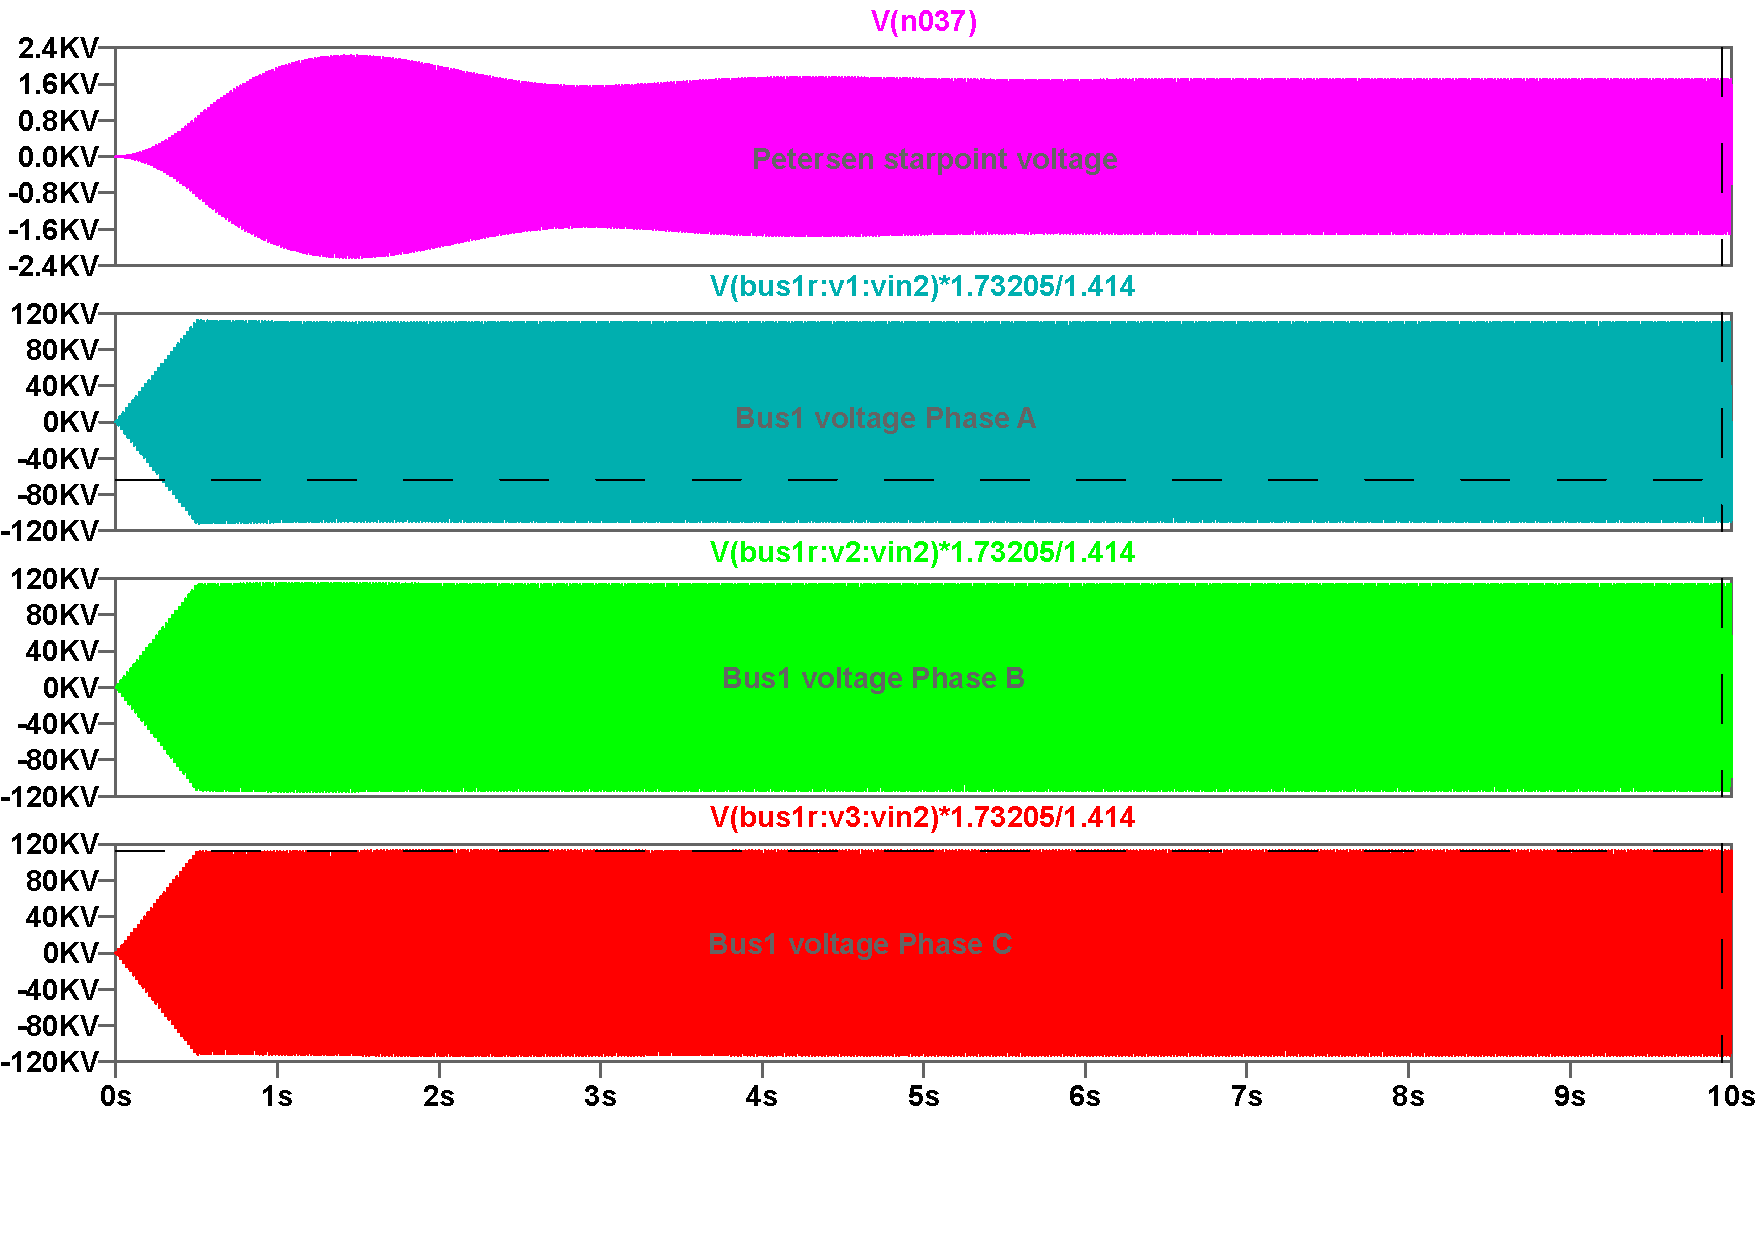
\includegraphics[width=0.90\textwidth]{figures/06_Switching_on_networks/Switching_on_networks_Bus0_Bus1_voltages-case9}
	\caption{Switching on networks voltage-trip, voltages - case9}
	\label{fig:figure625}
\end{figure}

\begin{figure}[H]
	\centering
	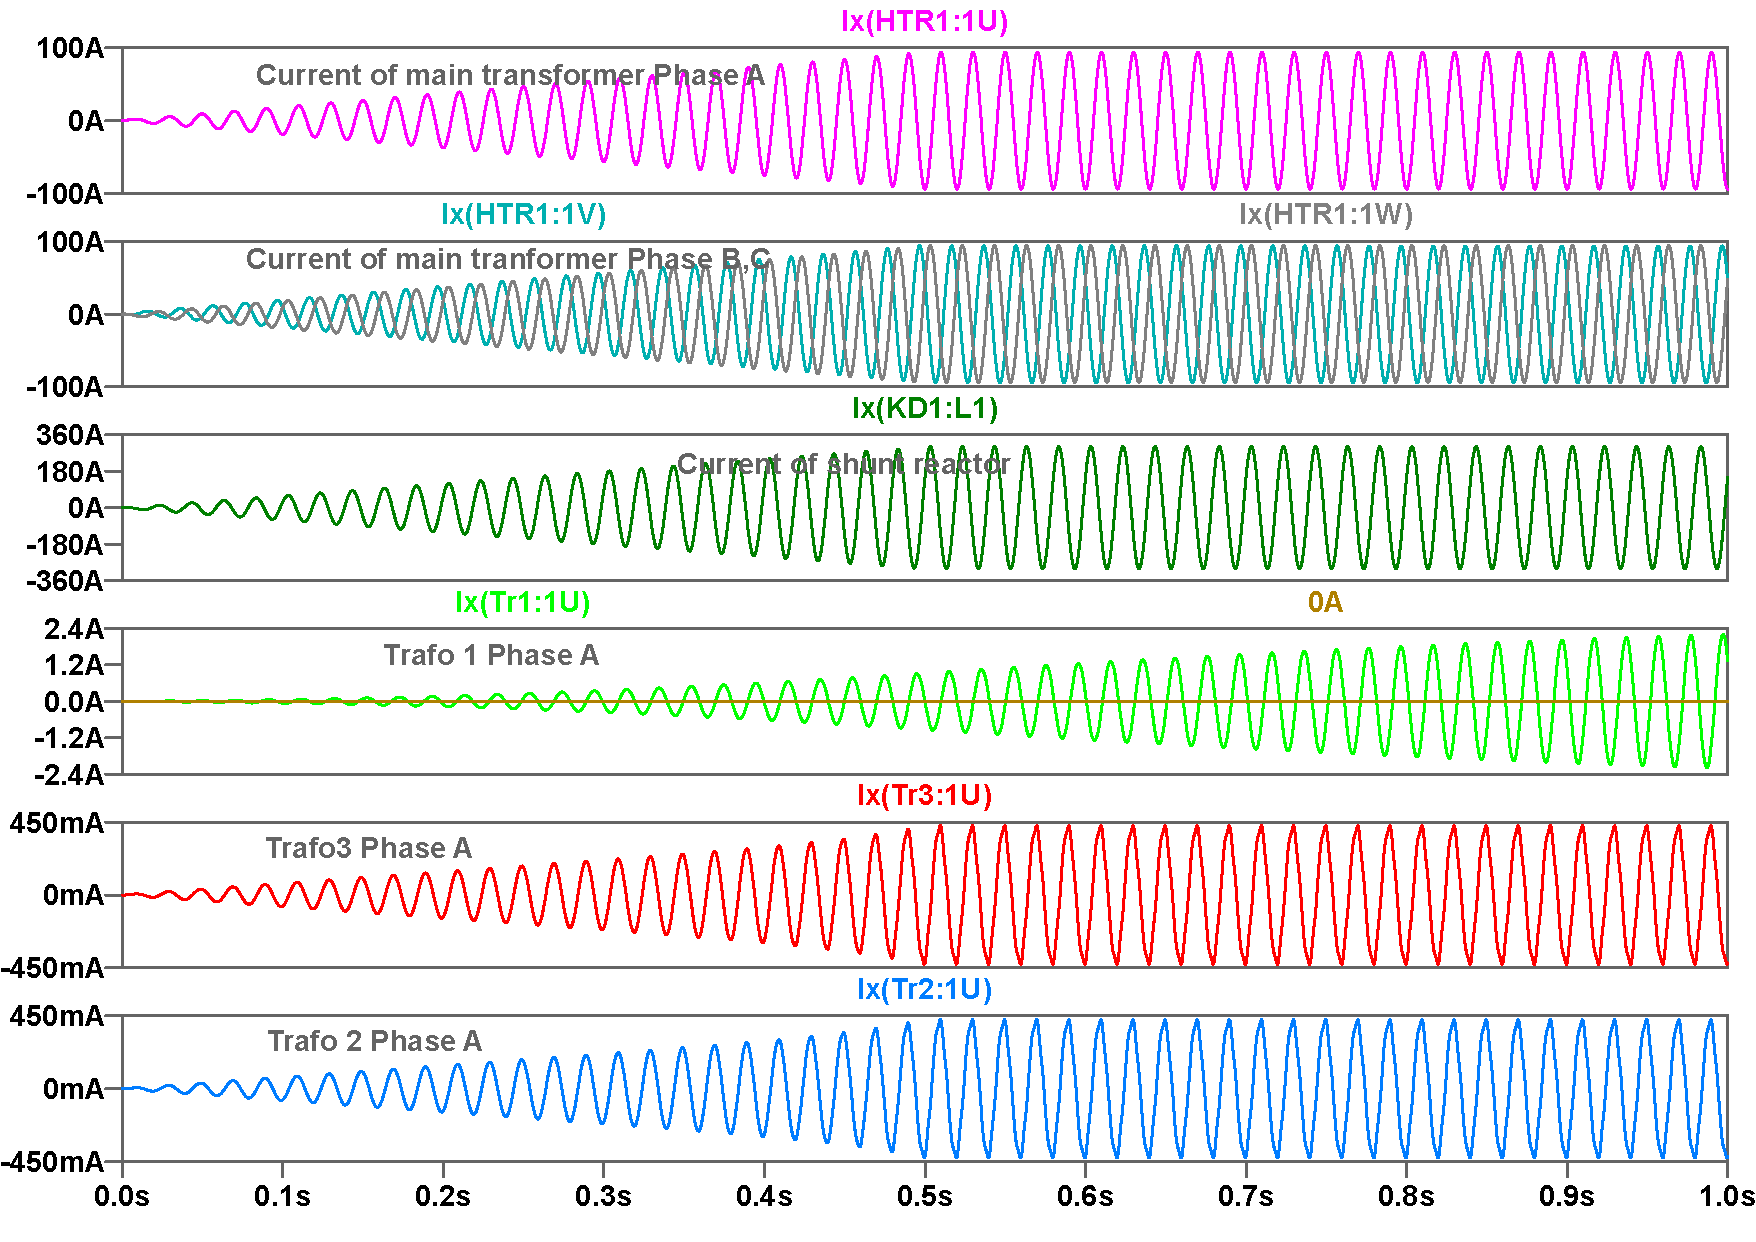
\includegraphics[width=0.90\textwidth]{figures/06_Switching_on_networks/Switching_on_networks_currents-case9}
	\caption{Switching on networks voltage-trip, currents - case9}
	\label{fig:figure626}
\end{figure}

\begin{figure}[H]
	\centering
	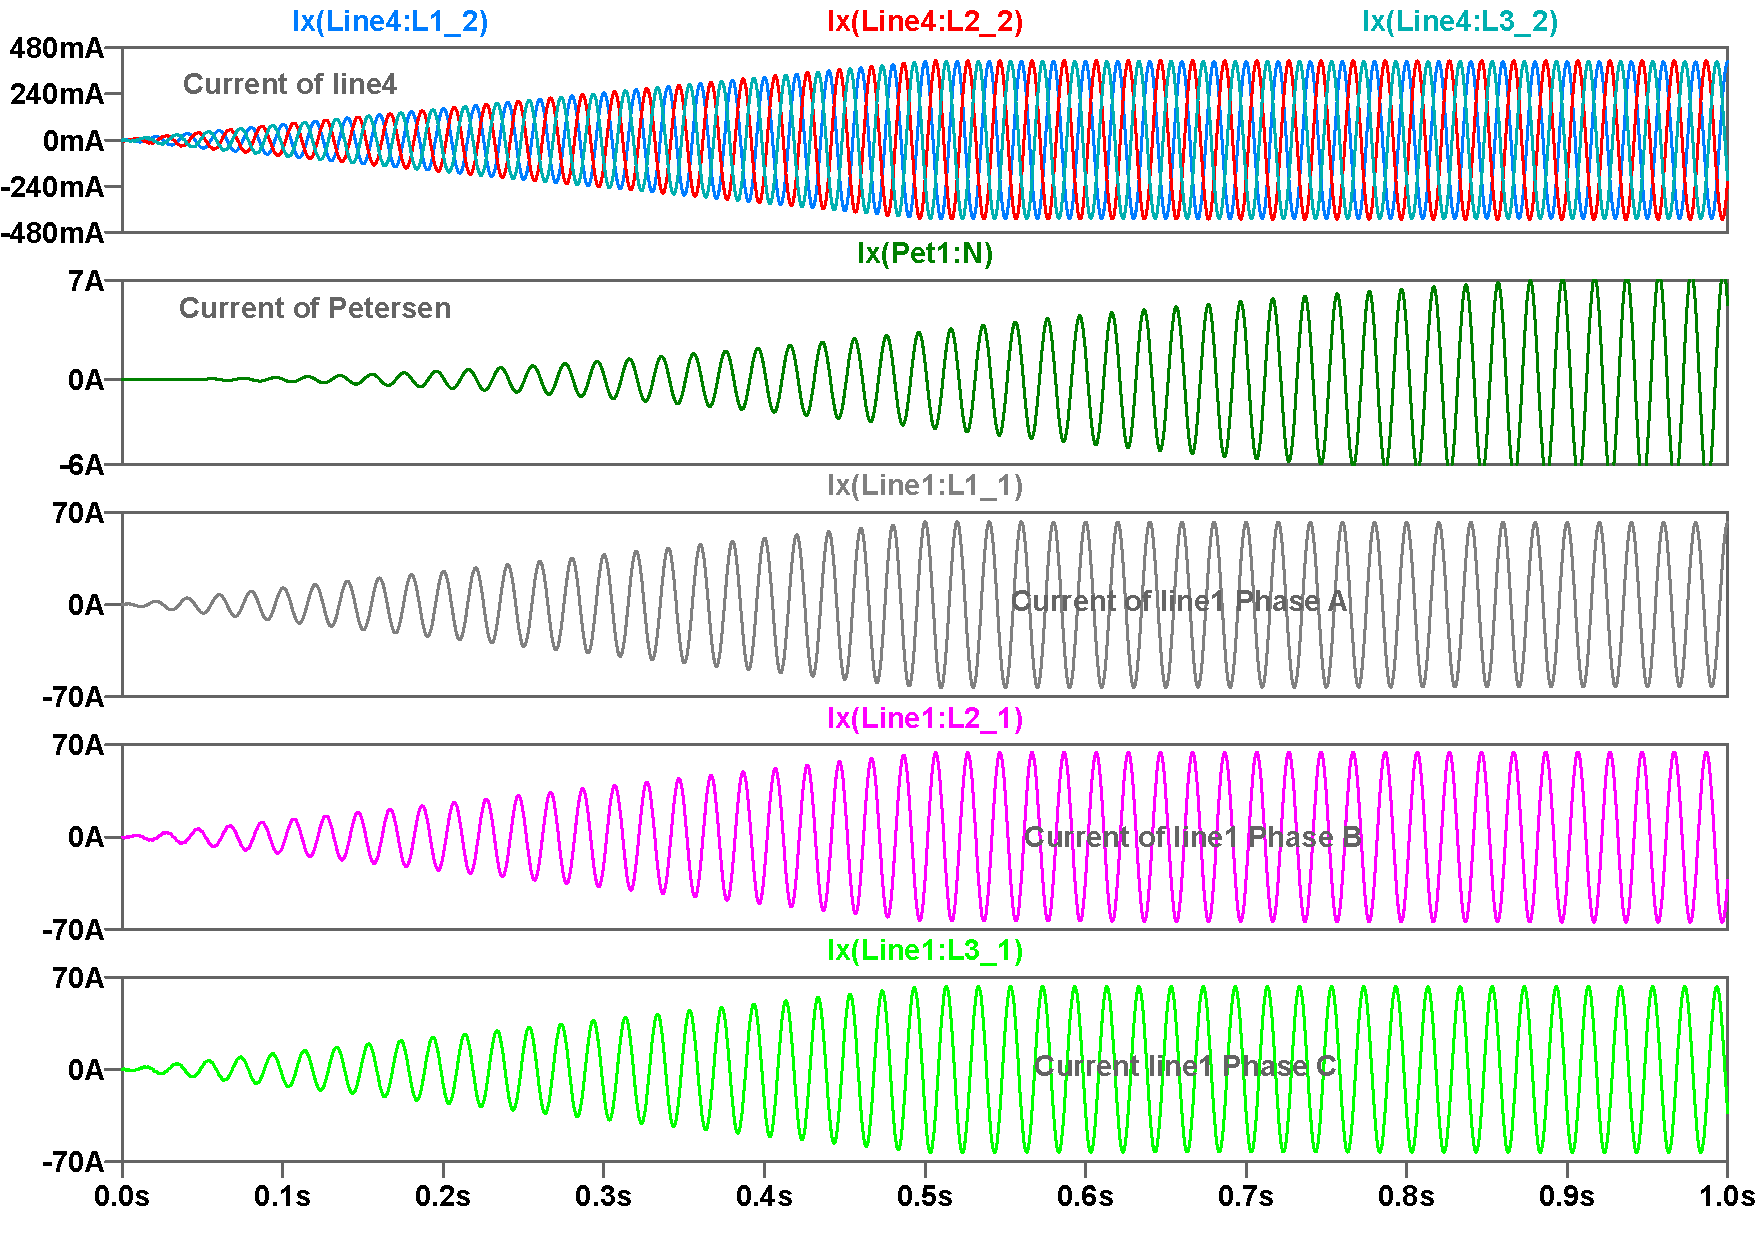
\includegraphics[width=0.90\textwidth]{figures/06_Switching_on_networks/Switching_on_networks_currents_Line1_Line4-case9}
	\caption{Switching on networks voltage-trip, currents line1, line4 - case9}
	\label{fig:figure627}
\end{figure}

\begin{figure}[H]
	\centering
	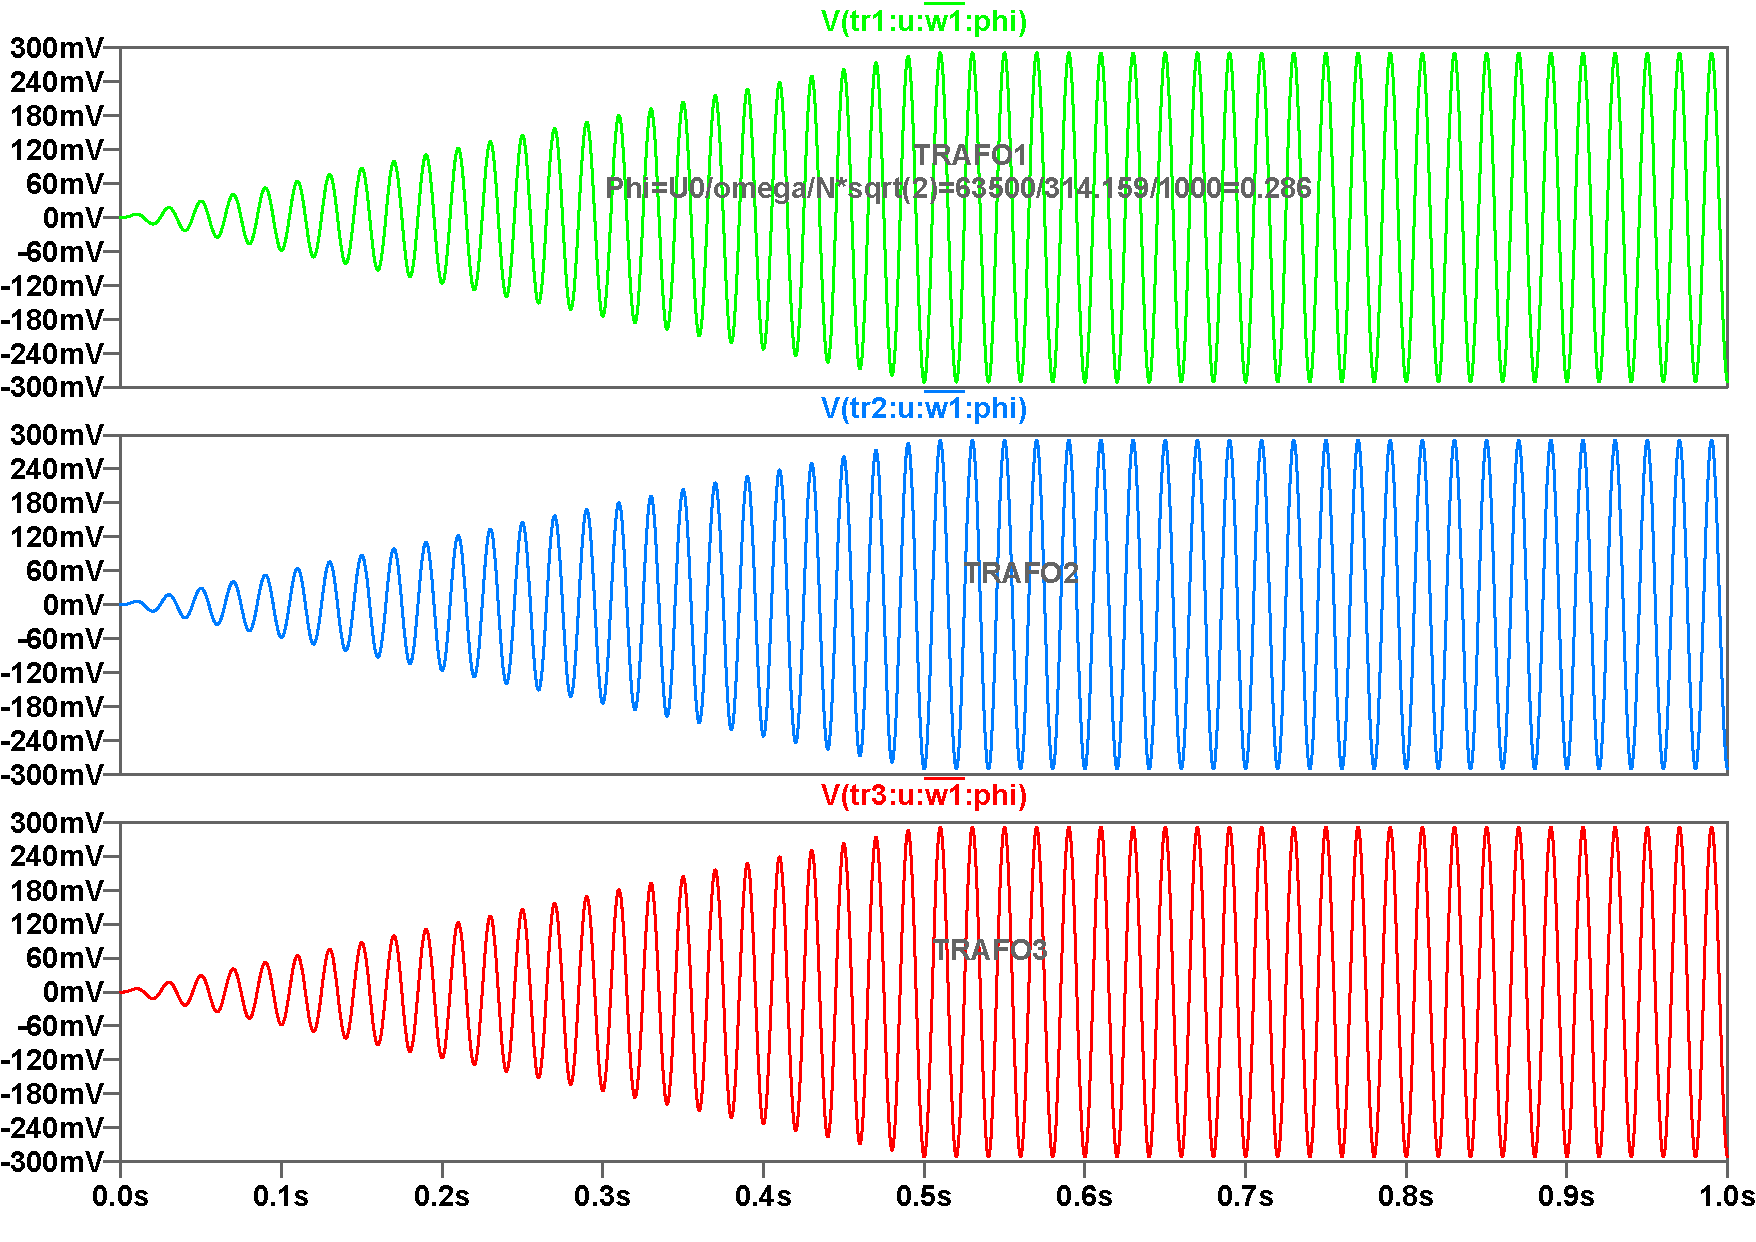
\includegraphics[width=0.90\textwidth]{figures/06_Switching_on_networks/Switching_on_networks_phi-case9}
	\caption{Switching on networks voltage-trip, fluxes - case9}
	\label{fig:figure628}
\end{figure}

\begin{figure}[H]
	\centering
	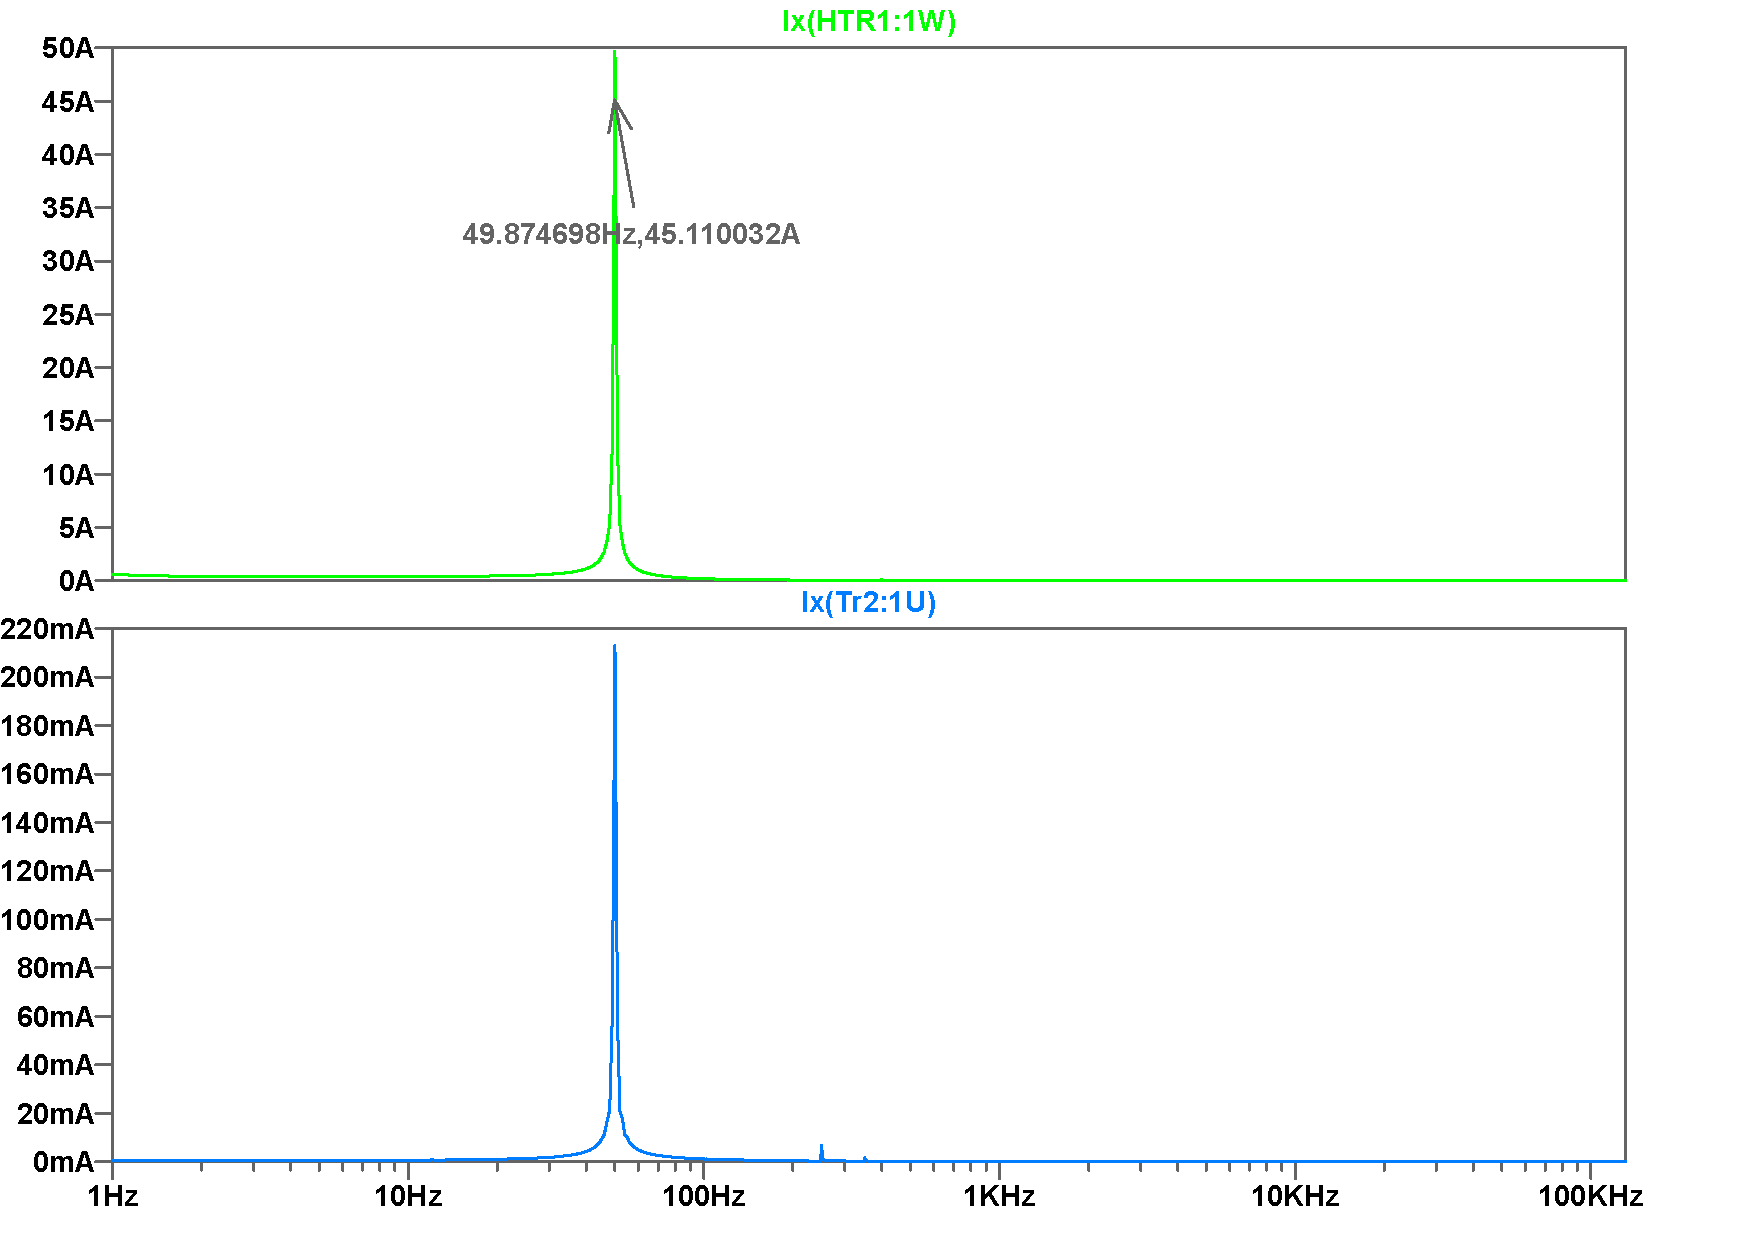
\includegraphics[width=0.90\textwidth]{figures/06_Switching_on_networks/Switching_on_networks_FFT_Transformer-case9}
	\caption{Switching on networks voltage-trip, FFT - case9}
	\label{fig:figure629}
\end{figure}


% Measurement values table for the Power System Simulation book.
% Required packages are already loaded by the central preamble:
% booktabs, tabularx, array, siunitx, xcolor.

\begin{table}[htbp]
  \centering
  \caption{Signal ranges for Case 9. All values are peak values, bus values are multiplied by 1.73/1.414}
  \label{tab:measurement-values-case9}
  \small
  \setlength{\tabcolsep}{3.5pt}
  \renewcommand{\arraystretch}{1.18}
  \begin{tabularx}{\textwidth}{@{}
      >{\raggedright\arraybackslash}p{0.055\textwidth}
      >{\raggedright\arraybackslash}p{0.085\textwidth}
      >{\raggedright\arraybackslash}p{0.095\textwidth}
      >{\raggedright\arraybackslash}p{0.105\textwidth}
      >{\raggedright\arraybackslash}p{0.075\textwidth}
      >{\raggedright\arraybackslash}p{0.075\textwidth}
      Y@{}}
    \toprule
    \textbf{Meas.} &
    \textbf{Grid element} &
    \textbf{Phase} &
    \textbf{Voltage level} &
    \textbf{Min.} &
    \textbf{Max.} &
    \textbf{Notes} \\
    \midrule
    $V$ & Bus0  & Ph A       & \SI{220}{\kilo\volt} & \SI{-229}{\kilo\volt} & \SI{229}{\kilo\volt} & Steady state RMS \\
    $V$ & Bus1  & Ph A       & \SI{110}{\kilo\volt} & \SI{-110}{\kilo\volt} & \SI{110}{\kilo\volt} & Steady state RMS \\
    $V$ & Bus1  & Ph B, C    & \SI{110}{\kilo\volt} & \SI{-113}{\kilo\volt} & \SI{113}{\kilo\volt} & Steady state RMS \\
    $I$ & HTr1  & Ph A       & \SI{220}{\kilo\volt} & \SI{-94}{\ampere} & \SI{94}{\ampere} & Steady state peak \\
    $I$ & HTr1  & Ph B, C    & \SI{220}{\kilo\volt} & \SI{-94}{\ampere} & \SI{94}{\ampere} & Steady state peak \\
    $I$ & KD1   & Ph A       & \SI{110}{\kilo\volt} & \SI{-300}{\ampere} & \SI{300}{\ampere} & Steady state peak \\
    $I$ & Tr1   & Ph A       & \SI{110}{\kilo\volt} & \SI{-2}{\ampere} & \SI{2}{\ampere} & Due to Petersen higher than Tr2,3 \\
    $I$ & Tr2   & Ph A       & \SI{110}{\kilo\volt} & \SI{-450}{\milli\ampere} & \SI{450}{\milli\ampere} & Steady state zero load peak current \\
    $I$ & Tr3   & Ph A      & \SI{110}{\kilo\volt} & \SI{-450}{\milli\ampere} & \SI{450}{\milli\ampere} & Steady state zero load peak current \\
    $I$ & Line4 & Ph A & \SI{110}{\kilo\volt} & \SI{-410}{\milli\ampere} & \SI{410}{\milli\ampere} & Steady state peak   \\
    $I$ & Line1 & Ph A, B, C & \SI{110}{\kilo\volt} & \SI{-62}{\ampere} & \SI{62}{\ampere} & Steady state peak  \\
    $I$ & Pet1 & Ph N & \SI{110}{\kilo\volt} & \SI{-7}{\ampere} & \SI{7}{\ampere} & Steady state peak \\
    $V$ & Pet1 & Ph N & \SI{110}{\kilo\volt} & \SI{-1.7}{\kilo\volt} & \SI{1.7}{\kilo\volt} & Steady state peak \\
    $\Phi$ & Tr1 & Ph A, B, C   & \SI{110}{\kilo\volt} & \SI{0.291}{\weber} & \SI{0.291}{\weber} & Nominal flux: \SI{0.288}{\weber} peak \\
    FFT & HTr1  & Ph C       & \SI{220}{\kilo\volt} & \SI{50}{\hertz} & \SI{50}{\hertz} & only \SI{50}{\hertz} nominal frequ.  \\
    FFT & Tr2   & Ph A       & \SI{110}{\kilo\volt} & \SI{50}{\hertz} & \SI{50}{\hertz} & \SI{50}{\hertz} nominal frequ. \\     
    \bottomrule
  \end{tabularx}
\end{table}





\begin{important}{Preferred energization method}{imp:network-voltage-ramp}
A controlled voltage ramp avoids the abrupt change in applied voltage that
excites cable resonances and transformer flux offsets. The ramp time must be
long compared with the dominant electrical oscillation periods, and load
connection must be delayed until the voltage is established.
\end{important}

\begin{chaptersummary}
Energizing an entire cable-dominated network excites both transformer inrush
and cable-charging transients. The switching instant determines which phases
are dominated by magnetizing current and which by capacitive current. Cable
capacitance, referred transformer inductance, tap position, load, and network
strength determine the natural frequencies and transient amplitudes. Residual
flux can raise transformer currents above rated peak current, while connected
loads add effective damping. In this study, a gradual source-voltage ramp is
the most effective energization method because it suppresses both cable
resonances and transformer inrush.
\end{chaptersummary}

\chapter{Coupled Lines with Resonance}
\label{chap:coupled-lines-resonance}
\index{coupled lines}
\index{resonance!parallel overhead lines}
\index{line transposition}
\index{inductive compensation}

\section{General}
\label{sec:coupled-lines-general}

This chapter investigates two electromagnetically coupled
\SI{400}{\kilo\volt} overhead lines on a common Danube-type tower. 
The capacitive reactive power of the two lines is compensated by an inductive choke. We will examine the case where the compensation is near ideal—that is, where the inductive reactive power of the choke compensates for the capacitive reactive power of the line.
The following cases are simulated (Line 1 is always energized):

\begin{itemize}
	\item \texttt{Line 2 is open (lines are untransposed)},
	\item \texttt{Line 2 is open (lines are transposed)},
	\item \texttt{Line 2 is initially grounded and then ungrounded},
	\item \texttt{Line 2 is initially energized and then switched off},
	\item \texttt{Line 2 is initially energized and then switched off without a com-pensating reactor}
\end{itemize}

\section{Circuit design}
The total
line length is approximately \SI{9.75}{\kilo\metre}. Mutual inductances and
capacitances couple the circuits even when one line is disconnected at both
ends.

The per-kilometre inductance and capacitance matrices of the coupled line were calculated with ATP
and then stored in \texttt{line\_coupled.lib}.
The Excel file Lines\_and\_cables.xlsx assists with conversion to LTspice library code.

Each line is almost fully compensated by an shunt reactor
element, \texttt{l\_batt}. Near-exact compensation creates an important
operating condition: if line 1 is energized while line 2 is open at both ends,
the mutual coupling can excite a resonance and produce very high voltages on
the disconnected line.

\section{Determining the Compensation Rating}
\label{sec:coupled-line-compensation-rating}

Use \texttt{Coupled\_lines\_resonance\_TRAN.asc}. Save a working copy as
\texttt{test.asc}, remove the compensation elements, and run the transient
simulation. Measure the three phase reactive powers with
\texttt{qmeter\_uvw\_sgn}. The results are approximately

\begin{align}
Q_R&=\SI{-2.02}{\mega\varunit},&
Q_S&=\SI{-2.40}{\mega\varunit},&
Q_T&=\SI{-2.37}{\mega\varunit}.
\end{align}

The total capacitive reactive power is therefore approximately
\SI{-6.8}{\mega\varunit}. A compensation rating of
\SI{+6}{\mega\varunit} is selected for each line, leaving the system close to,
but not exactly at, resonance.

At \SI{400}{\kilo\volt}, the corresponding balanced three-phase current is

\begin{calculation}{Current of the \SI{6}{\mega\varunit} compensation reactor}{calculation71}
\begin{align}
I_{\mathrm{rms}}
 &=\frac{Q}{\sqrt{3}U_{\mathrm{LL}}}
   =\frac{\SI{6}{\mega\varunit}}
          {\sqrt{3}\cdot\SI{400}{\kilo\volt}}
   \approx\SI{8.66}{\ampere},\\
\widehat I&=\sqrt{2}\,I_{\mathrm{rms}}
   \approx\boxed{\SI{12.2}{\ampere}}.
\end{align}
\end{calculation}

\section{Line 1 Energized and Line 2 Open: Untransposed Lines} figures: \ref{fig:figure72}-\ref{fig:figure73}  (simulation-file: same name as the heading)
\label{sec:coupled-lines-open-untransposed}

Line 1 is supplied by a source with an exponential voltage startup, while line 2 remains
open at both ends. The open-line voltages exhibit a slow beat and approach
their final values after approximately \SI{2}{\second}.

Phase A of line 2 has the highest voltage, with transient peaks near
\SI{500}{\kilo\volt}, corresponding to approximately
\SI{350}{\kilo\volt} RMS. The other two phase peaks remain below
\SI{300}{\kilo\volt}. For comparison, the normal phase-voltage peak of the
energized \SI{400}{\kilo\volt} line is

\begin{equation}
\widehat U_{\mathrm{ph}}
 =\sqrt{2}\frac{U_{\mathrm{LL}}}{\sqrt{3}}
 =\sqrt{2}\frac{\SI{400}{\kilo\volt}}{\sqrt{3}} 
 \approx\SI{326.6}{\kilo\volt} peak.
\end{equation}

The settled phase A peak on line 2 is approximately
\SI{350}{\kilo\volt}, exceeding the normal phase-voltage peak of 327 kV on line 1 with \SI{327}{\kilo\volt} . The slow
envelope is caused by the small difference between the \SI{50}{\hertz} source
frequency and a nearby natural frequency formed by the line capacitances and
the compensating \texttt{l\_batt} reactors. 

The reactor-current peaks on line 1 are approximately
\SI{12}{\ampere} in all three phases, consistent with calculation \ref{calc:calculation71}. On line 2, the peak currents are
approximately \SI{13.3}{\ampere}, \SI{6}{\ampere}, and
\SI{7}{\ampere} in phases A, B, and C, respectively. The source currents are
close to zero because the line charging current is almost compensated.

The untransposed line has strongly unequal mutual capacitances and inductances.
Consequently, the phase magnitudes and phase angles on open line 2 are highly
asymmetric, and the sum of its three phase-to-earth voltages is nonzero, with a residual sum of approximately 46 kV.

\begin{figure}[H]
	\centering
	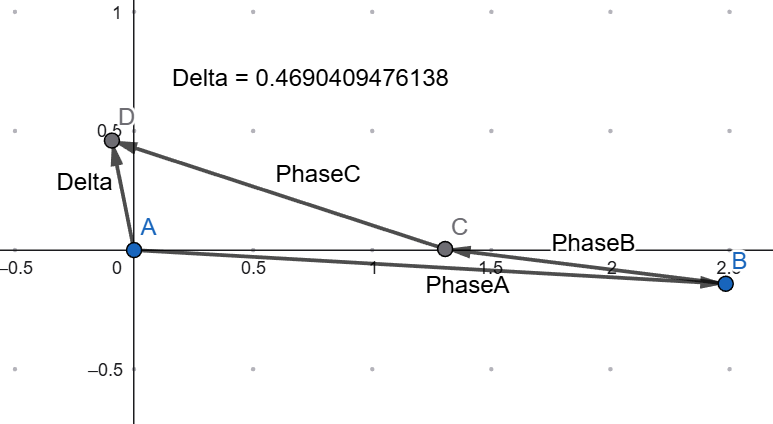
\includegraphics[width=0.8\textwidth]{figures/07_Coupled_lines_resonance/Sum_of_voltages_not_zero}
	\caption{Coupled lines resonance - Sum of voltages not zero - scale multiplied by 1e5}
	\label{fig:figure71}
\end{figure}


\begin{figure}[H]
	\centering
	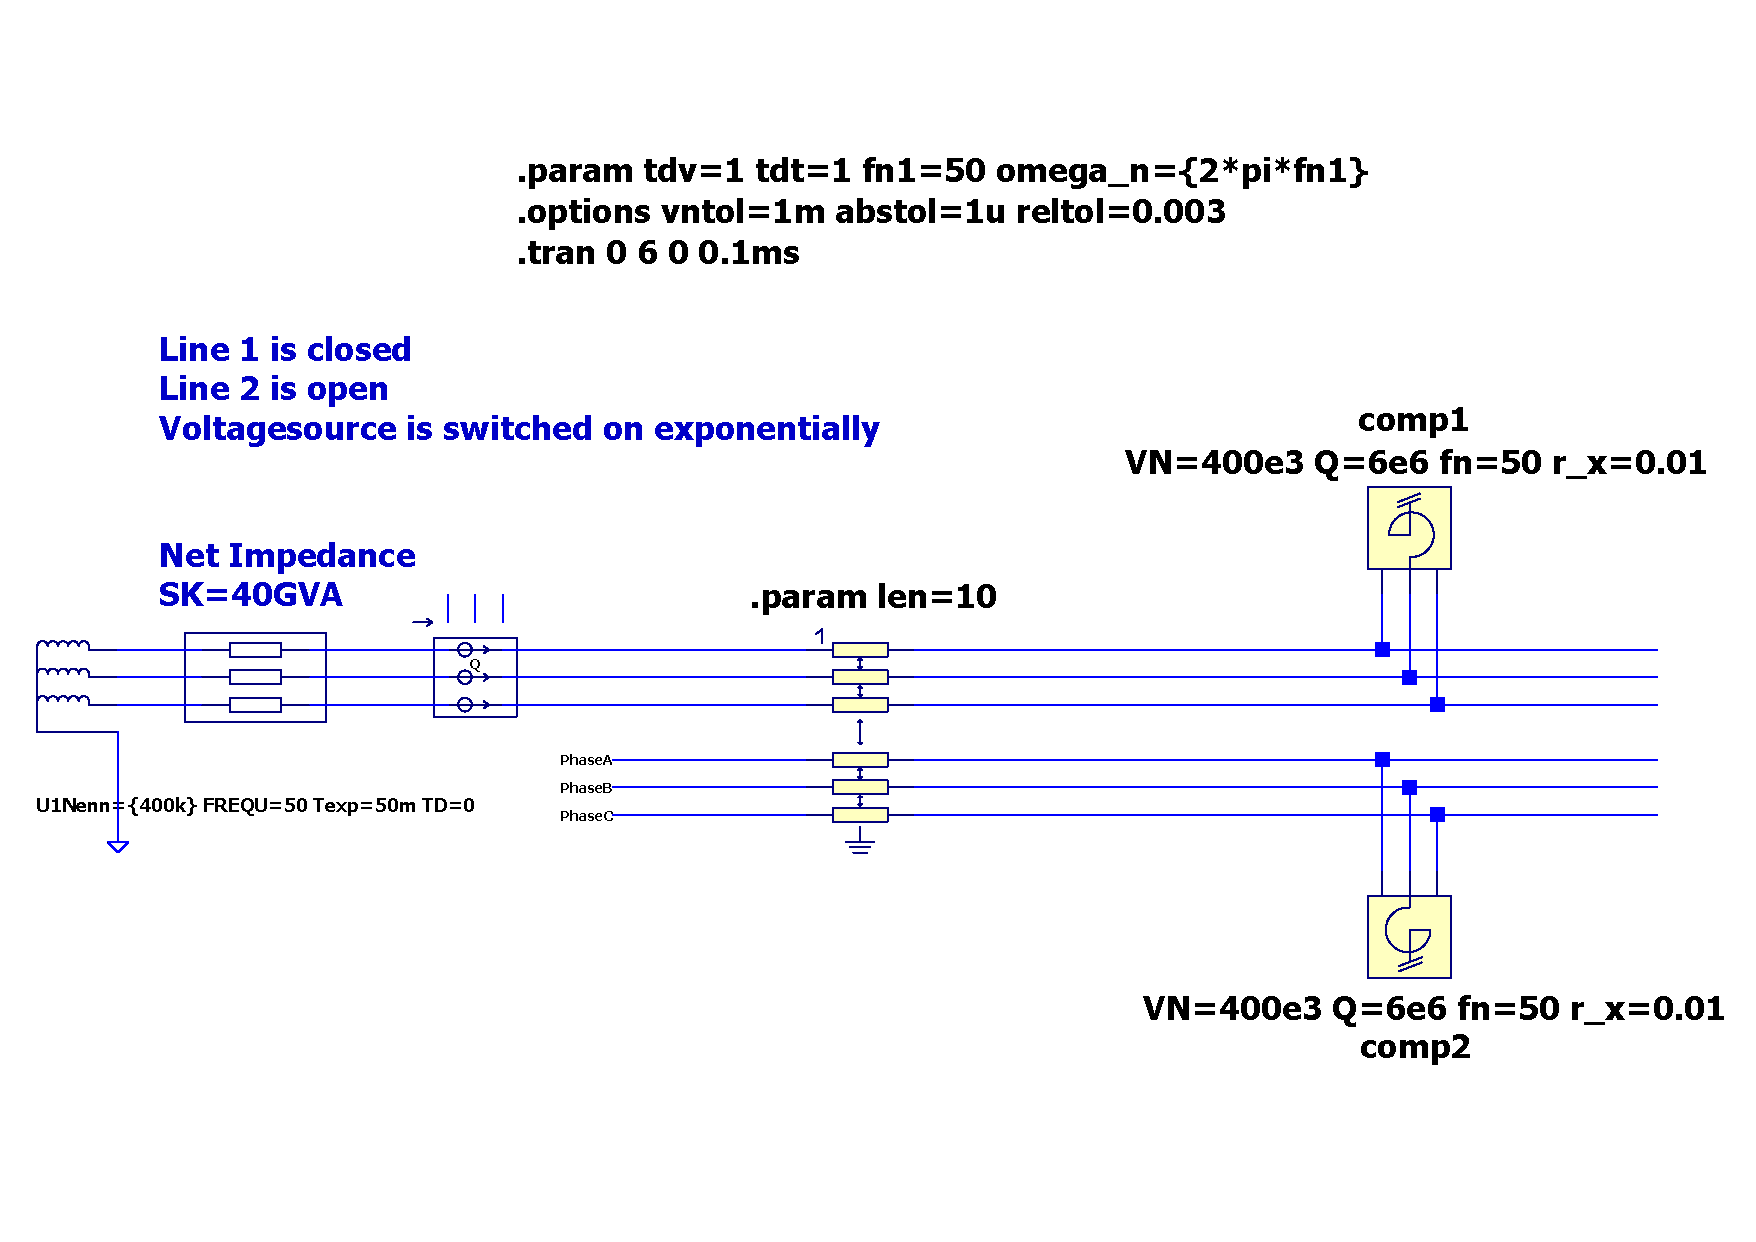
\includegraphics[width=1.0\textwidth]{figures/07_Coupled_lines_resonance/Coupled_lines_resonance_TRAN_schematic}
	\caption{Coupled lines resonance schematic - line2 is open untransposed TRAN analysis}
	\label{fig:figure72}
\end{figure}

\begin{figure}[H]
	\centering
	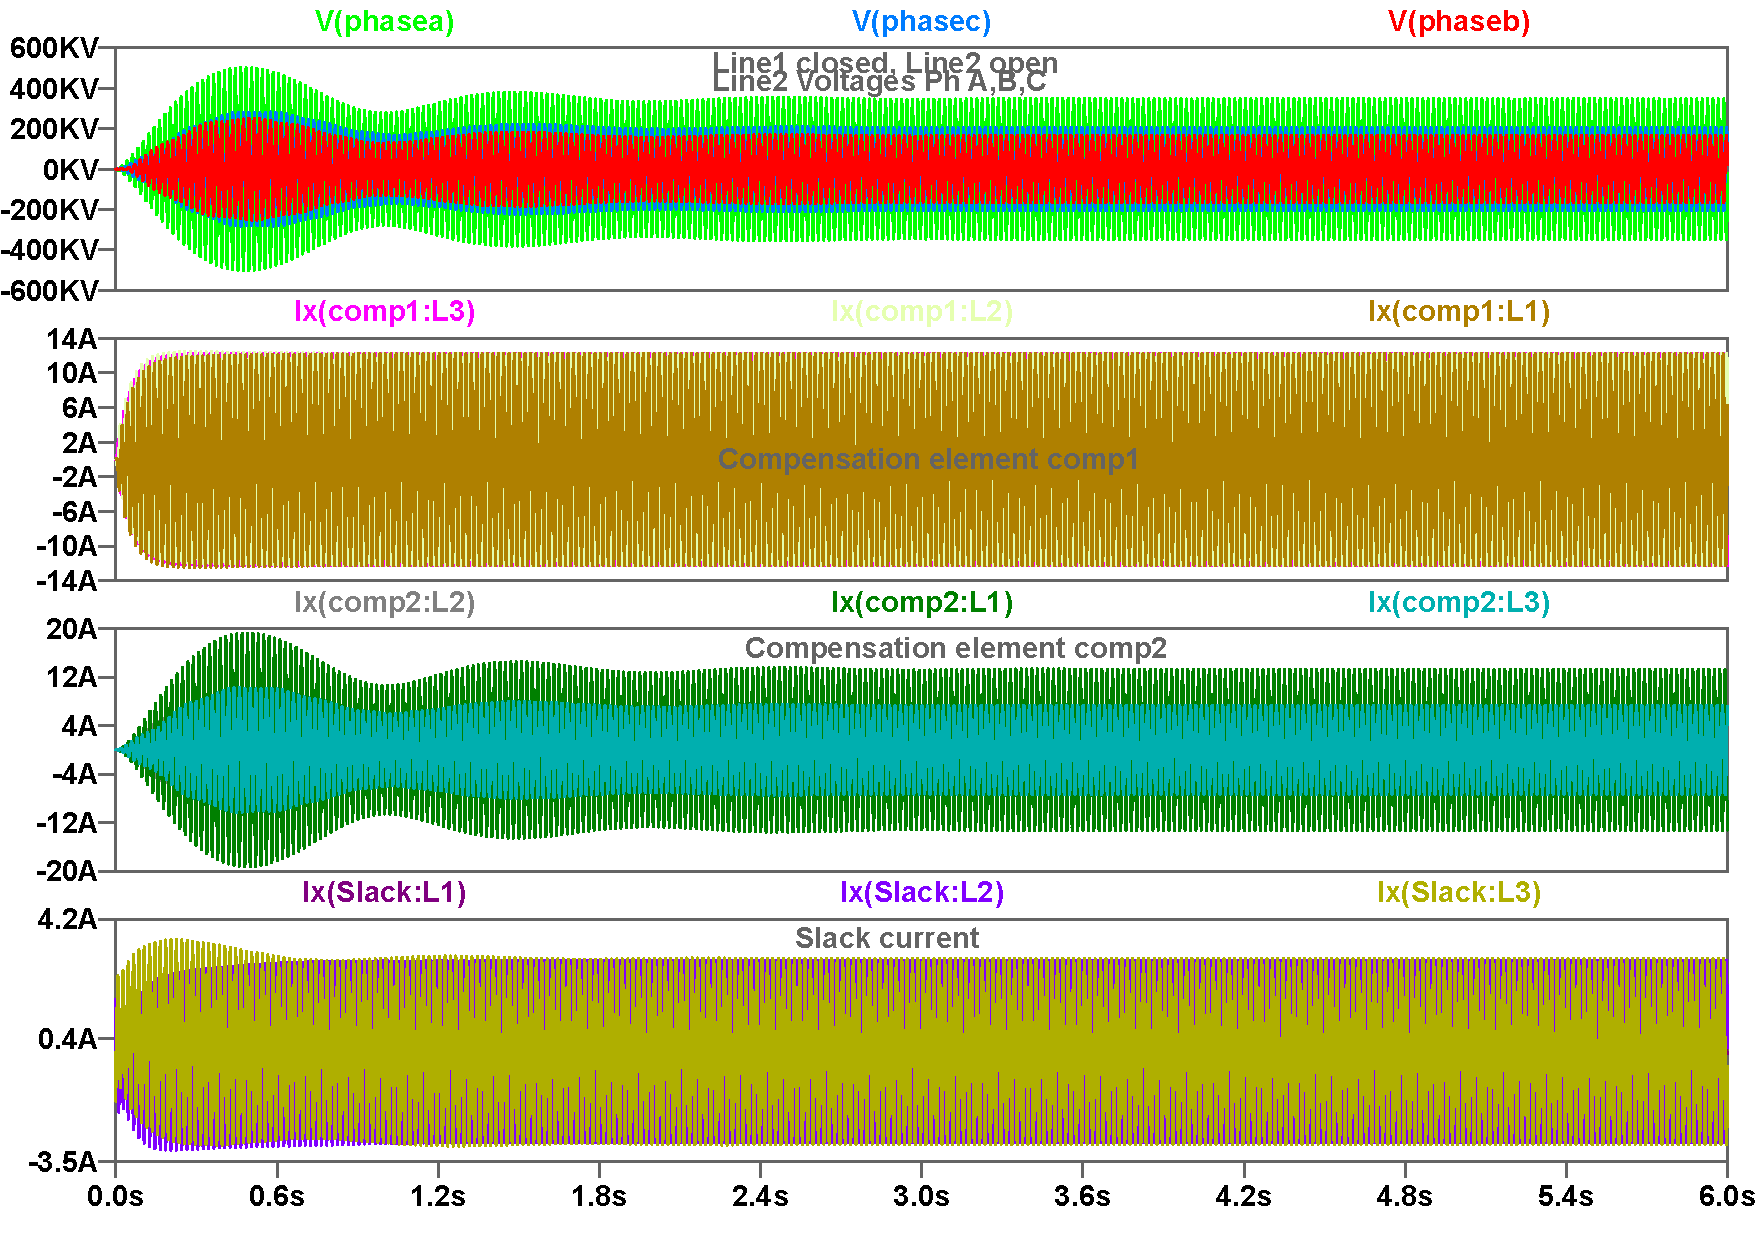
\includegraphics[width=0.90\textwidth]{figures/07_Coupled_lines_resonance/Coupled_lines_resonance_TRAN}
	\caption{Coupled lines resonance TRAN - line2 is open untransposed TRAN analysis}
	\label{fig:figure73}
\end{figure}


\section{AC Analysis of the Untransposed Open Line} figures: \ref{fig:figure74}-\ref{fig:figure75}  (simulation-file: same name as the heading) 
\label{sec:coupled-lines-ac-untransposed}

Set the vertical scale to linear by right-clicking the left axis. The principal
resonance of the open-line voltage lies near \SI{49}{\hertz}. At
\SI{50}{\hertz}, the phase-R voltage is approximately
\SI{250}{\kilo\volt} RMS, compared with the normal phase voltage of
approximately \SI{231}{\kilo\volt} RMS. This corresponds to the settled
transient value of approximately \SI{353}{\kilo\volt} peak.

A second resonance occurs near \SI{44}{\hertz}. At the main resonant peak near
\SI{49}{\hertz}, the Phase A voltage can approach approximately
\SI{1}{\mega\volt} peak. This demonstrates the sensitivity of the open coupled
line to small changes in shunt-reactor tuning.

\begin{important}{Near-resonant open-line overvoltage}{imp:coupled-line-resonance}
An open line is not necessarily de-energized when it shares a tower with an
energized line. Mutual capacitances and inductances can sustain a substantial
voltage, and near-resonant shunt compensation can amplify it far above the
normal phase voltage.
\end{important}

\subsection{Exercises}

\begin{enumerate}
\item Save the model as \texttt{test.asc} and increase the
      \texttt{l\_batt} rating until the resonant peak lies at
      \SI{50}{\hertz}. Observe the resulting voltage amplification.
\item Reduce the reactor rating to \SI{5}{\mega\varunit}. Compare the resonant
      frequency and peak magnitude with the original case.
\item Change the reactor parameter \texttt{r\_x}, which represents its ohmic
      component. Observe how increasing damping broadens and lowers the
      resonant peak.
\end{enumerate}

\section{Line 1 Energized and Line 2 Open: Transposed Lines} figures: \ref{fig:figure76}-\ref{fig:figure77}  (simulation-file: same name as the heading) 
\label{sec:coupled-lines-open-transposed}

Transposition makes the phase coupling approximately symmetrical. The three
open-line voltages therefore have equal magnitudes, and the relevant resonance
moves farther away from the power frequency.

The initial open-line peaks are approximately \SI{100}{\kilo\volt} and decay
to about \SI{70}{\kilo\volt} after \SI{2}{\second}. This is a substantially
more favourable operating condition than the untransposed case in
\cref{sec:coupled-lines-open-untransposed}.

\begin{remark}{Exercise}{imp:transposed-line-reactive-power}
	Save the model as \texttt{test.asc}, remove the \texttt{l\_batt} elements from
	both lines, and compare the phase currents and reactive powers of lines 1 and
	2. The transposed model should produce nearly symmetrical phase results.
\end{remark}

\begin{figure}[H]
	\centering
	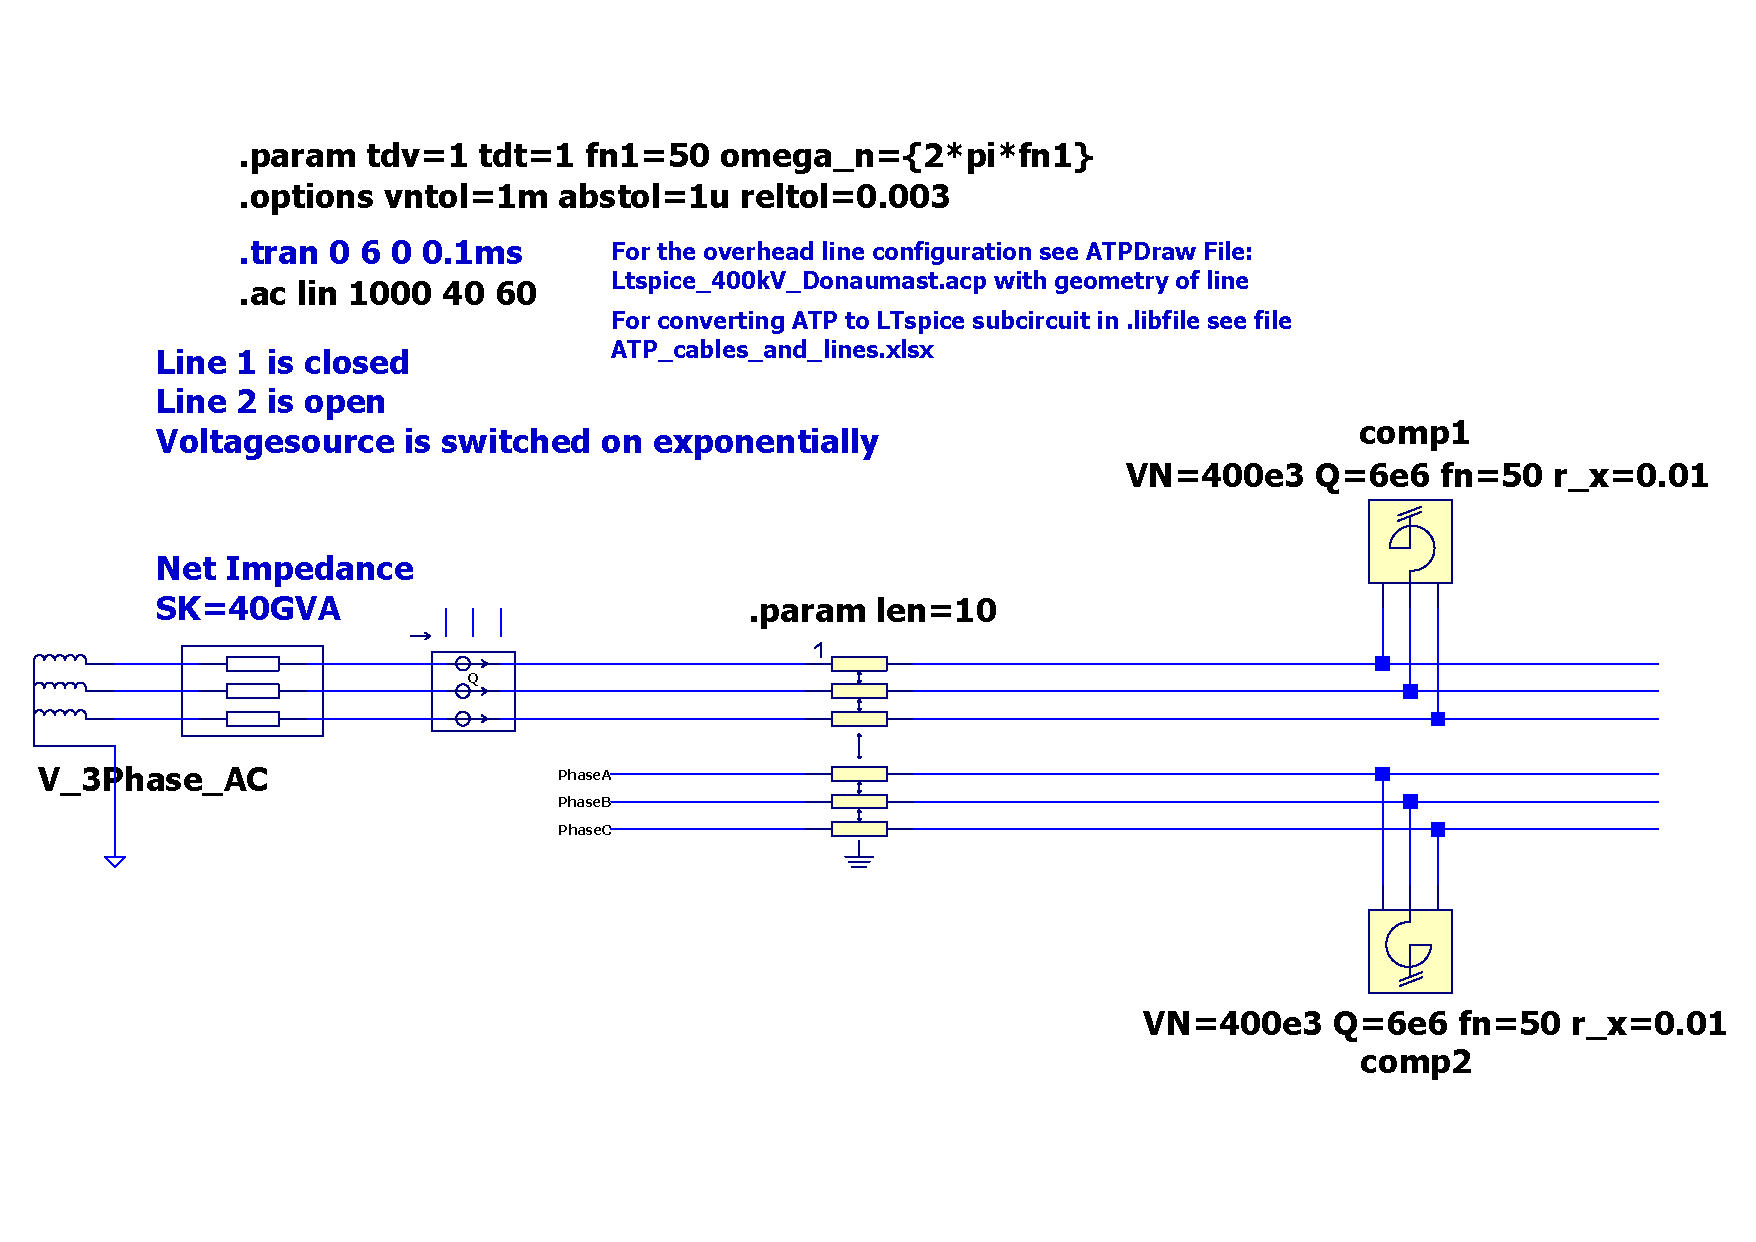
\includegraphics[width=1.0\textwidth]{figures/07_Coupled_lines_resonance/Coupled_lines_resonance_AC_schematic}
	\caption{Coupled lines resonance schematic - Lines2 is open untransposed AC analysis}
	\label{fig:figure74}
\end{figure}

\begin{figure}[H]
	\centering
	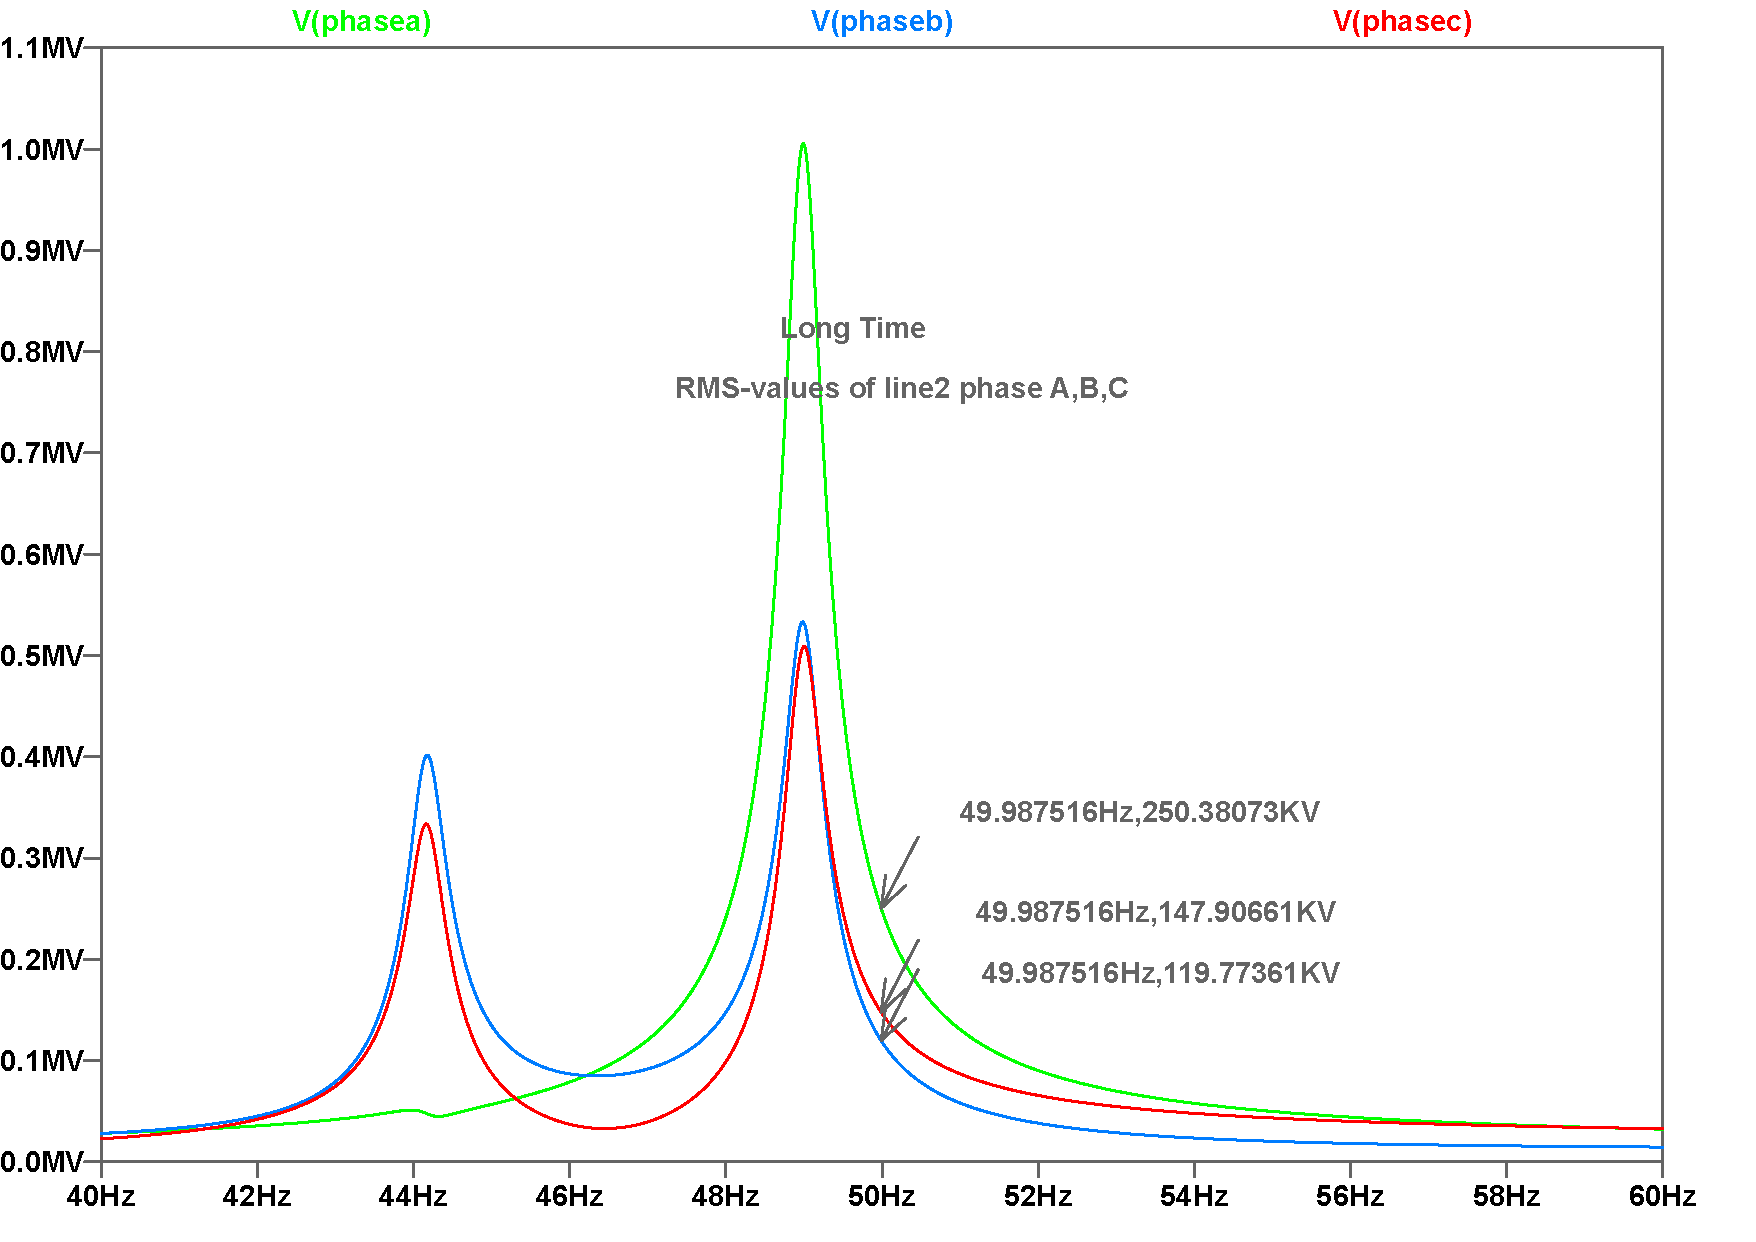
\includegraphics[width=0.90\textwidth]{figures/07_Coupled_lines_resonance/Coupled_lines_resonance_AC}
	\caption{Coupled lines resonance AC - Lines2 is open untransposed}
	\label{fig:figure75}
\end{figure}

\begin{figure}[H]
	\centering
	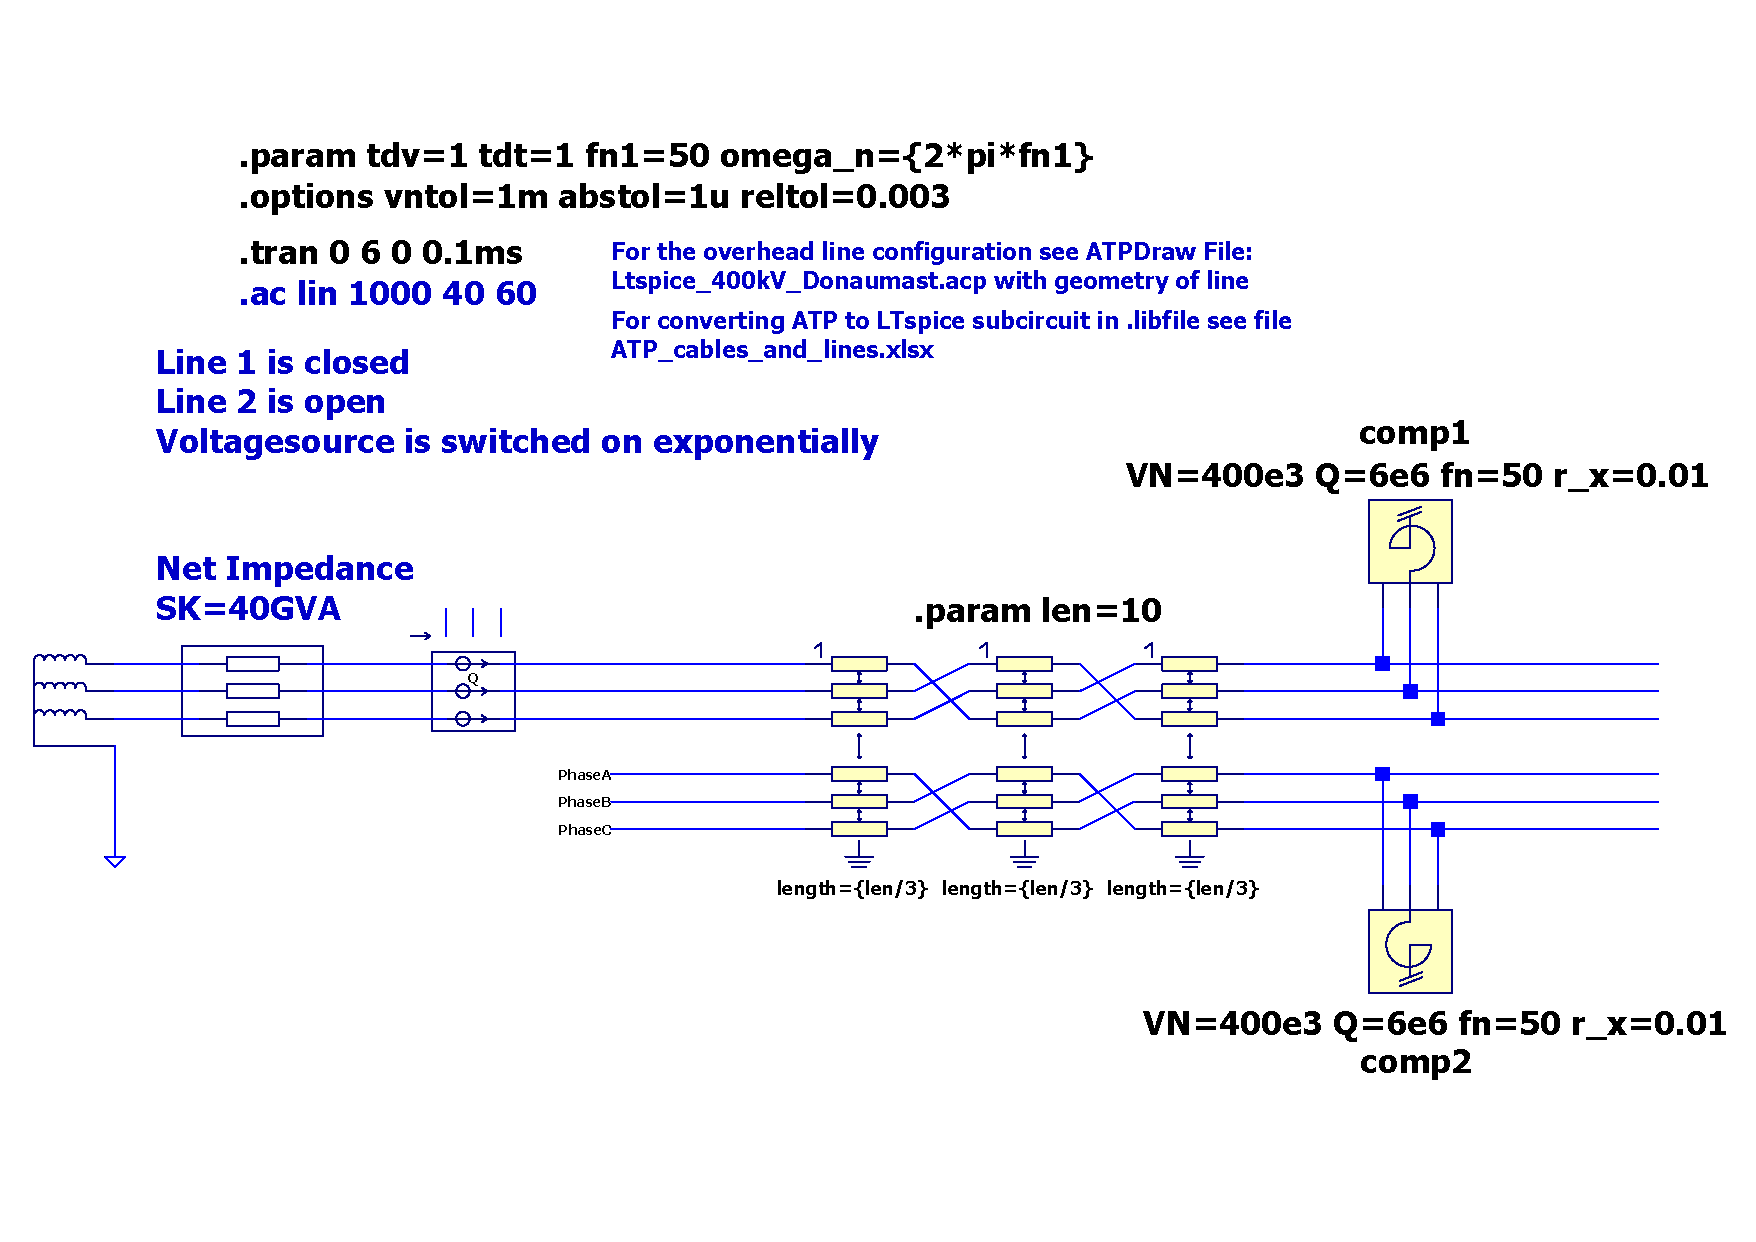
\includegraphics[width=1.0\textwidth]{figures/07_Coupled_lines_resonance/Coupled_lines_resonance_TRAN_transposed_schematic}
	\caption{Coupled lines resonance schematic - Lines2 is open transposed - TRAN analysis}
	\label{fig:figure76}
\end{figure}

\begin{figure}[H]
	\centering
	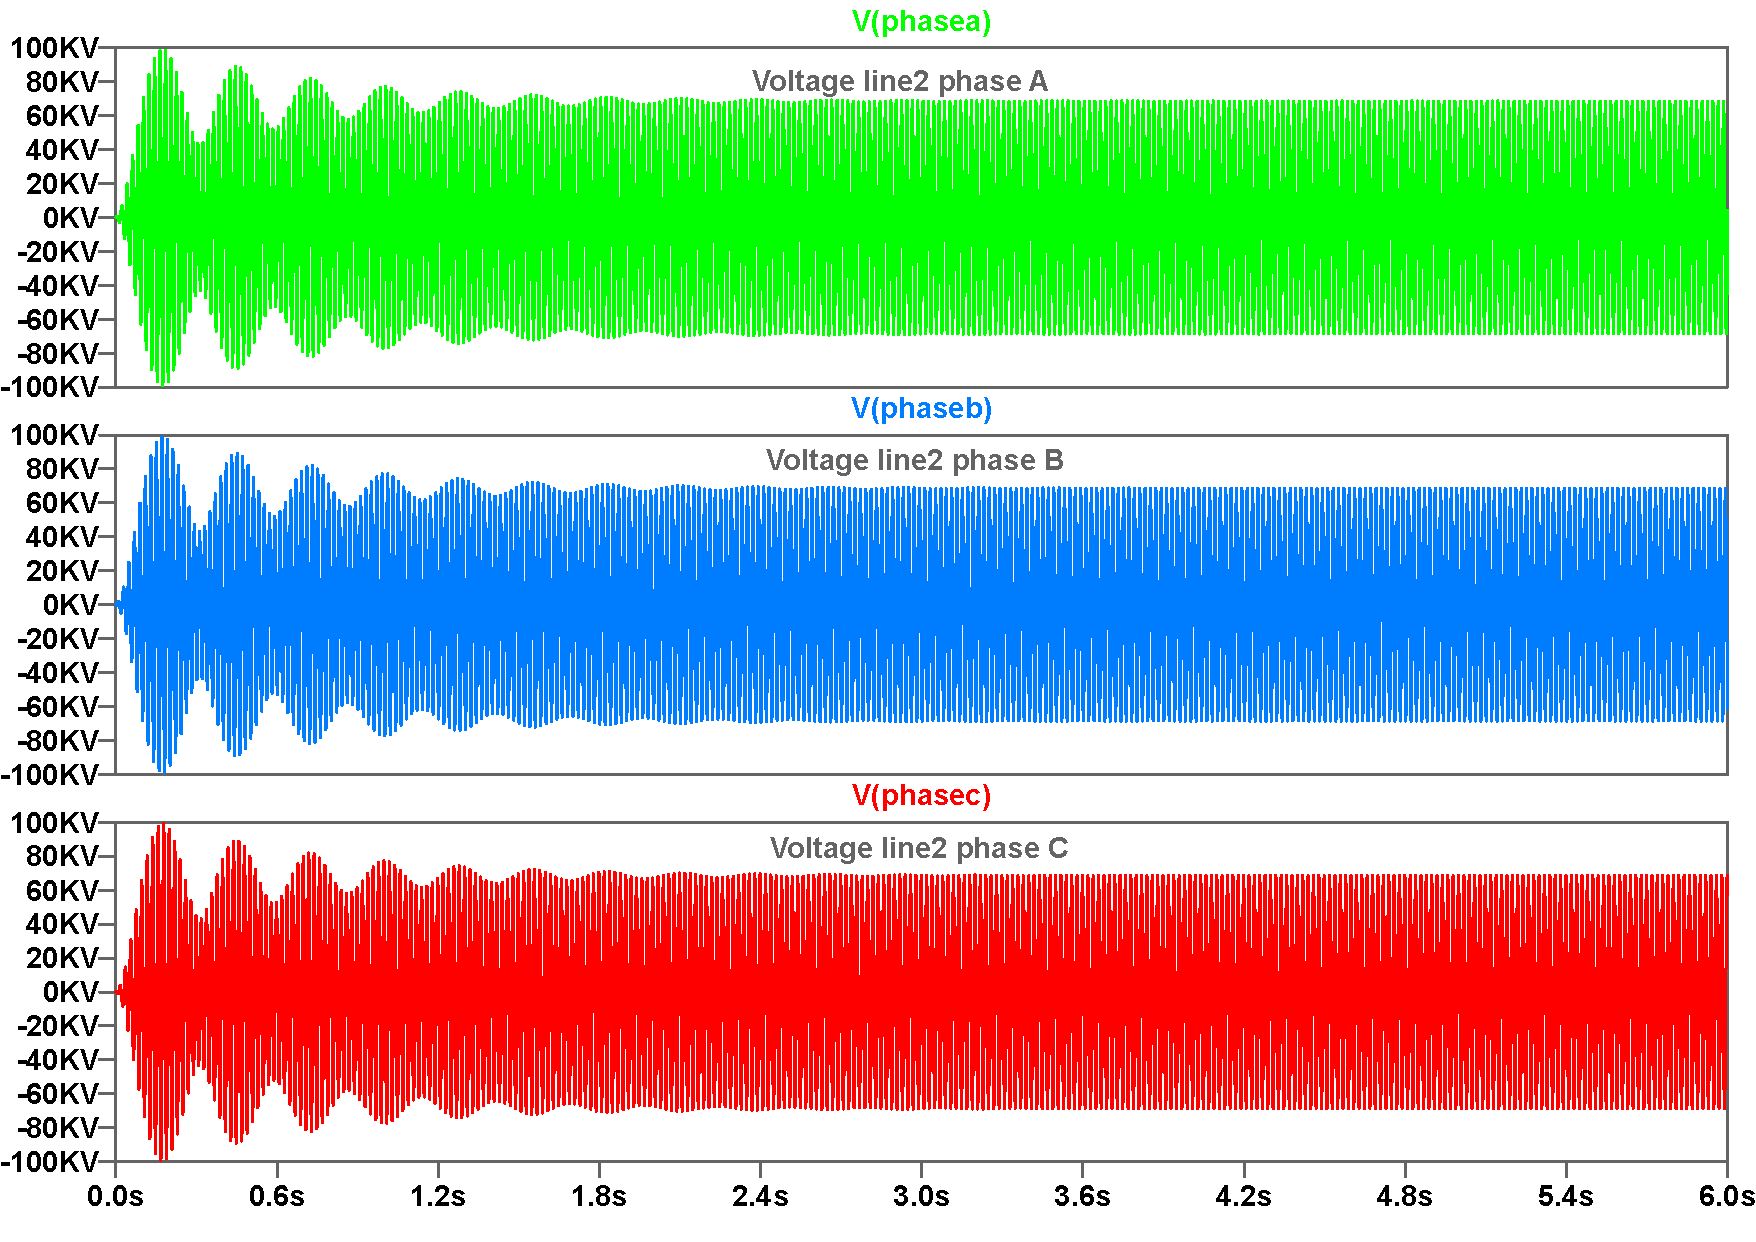
\includegraphics[width=0.90\textwidth]{figures/07_Coupled_lines_resonance/Coupled_lines_resonance_TRAN_transposed}
	\caption{Coupled lines resonance TRAN - Lines2 is open transposed}
	\label{fig:figure77}
\end{figure}

\section{AC Analysis of the Transposed Open Line} figures: \ref{fig:figure78}-\ref{fig:figure79}   (simulation-file: same name as the heading)
\label{sec:coupled-lines-ac-transposed}

The principal resonant peak shifts to approximately \SI{46.3}{\hertz}. The additional
lower-frequency maxima visible in the untransposed model disappear because
the phase coupling has been symmetrized. At \SI{50}{\hertz}, all three phase
voltages are approximately \SI{49}{\kilo\volt} RMS, or
\SI{70}{\kilo\volt} peak, in agreement with the final values of the transient
simulation.

\section{Line 2 Initially Grounded and Then Ungrounded} figures: \ref{fig:figure710}-\ref{fig:figure711}  (simulation-file: same name as the heading)
\label{sec:coupled-line-grounded-then-open}

Line 1 remains energized, while line 2 is initially grounded and subsequently opened.
The final response is similar to the permanently open case in
\cref{sec:coupled-lines-open-untransposed}. A second beat is particularly
visible in Phases A and B; it is associated with the second resonance near
\SI{44}{\hertz} identified by the AC analysis.

\begin{figure}[H]
	\centering
	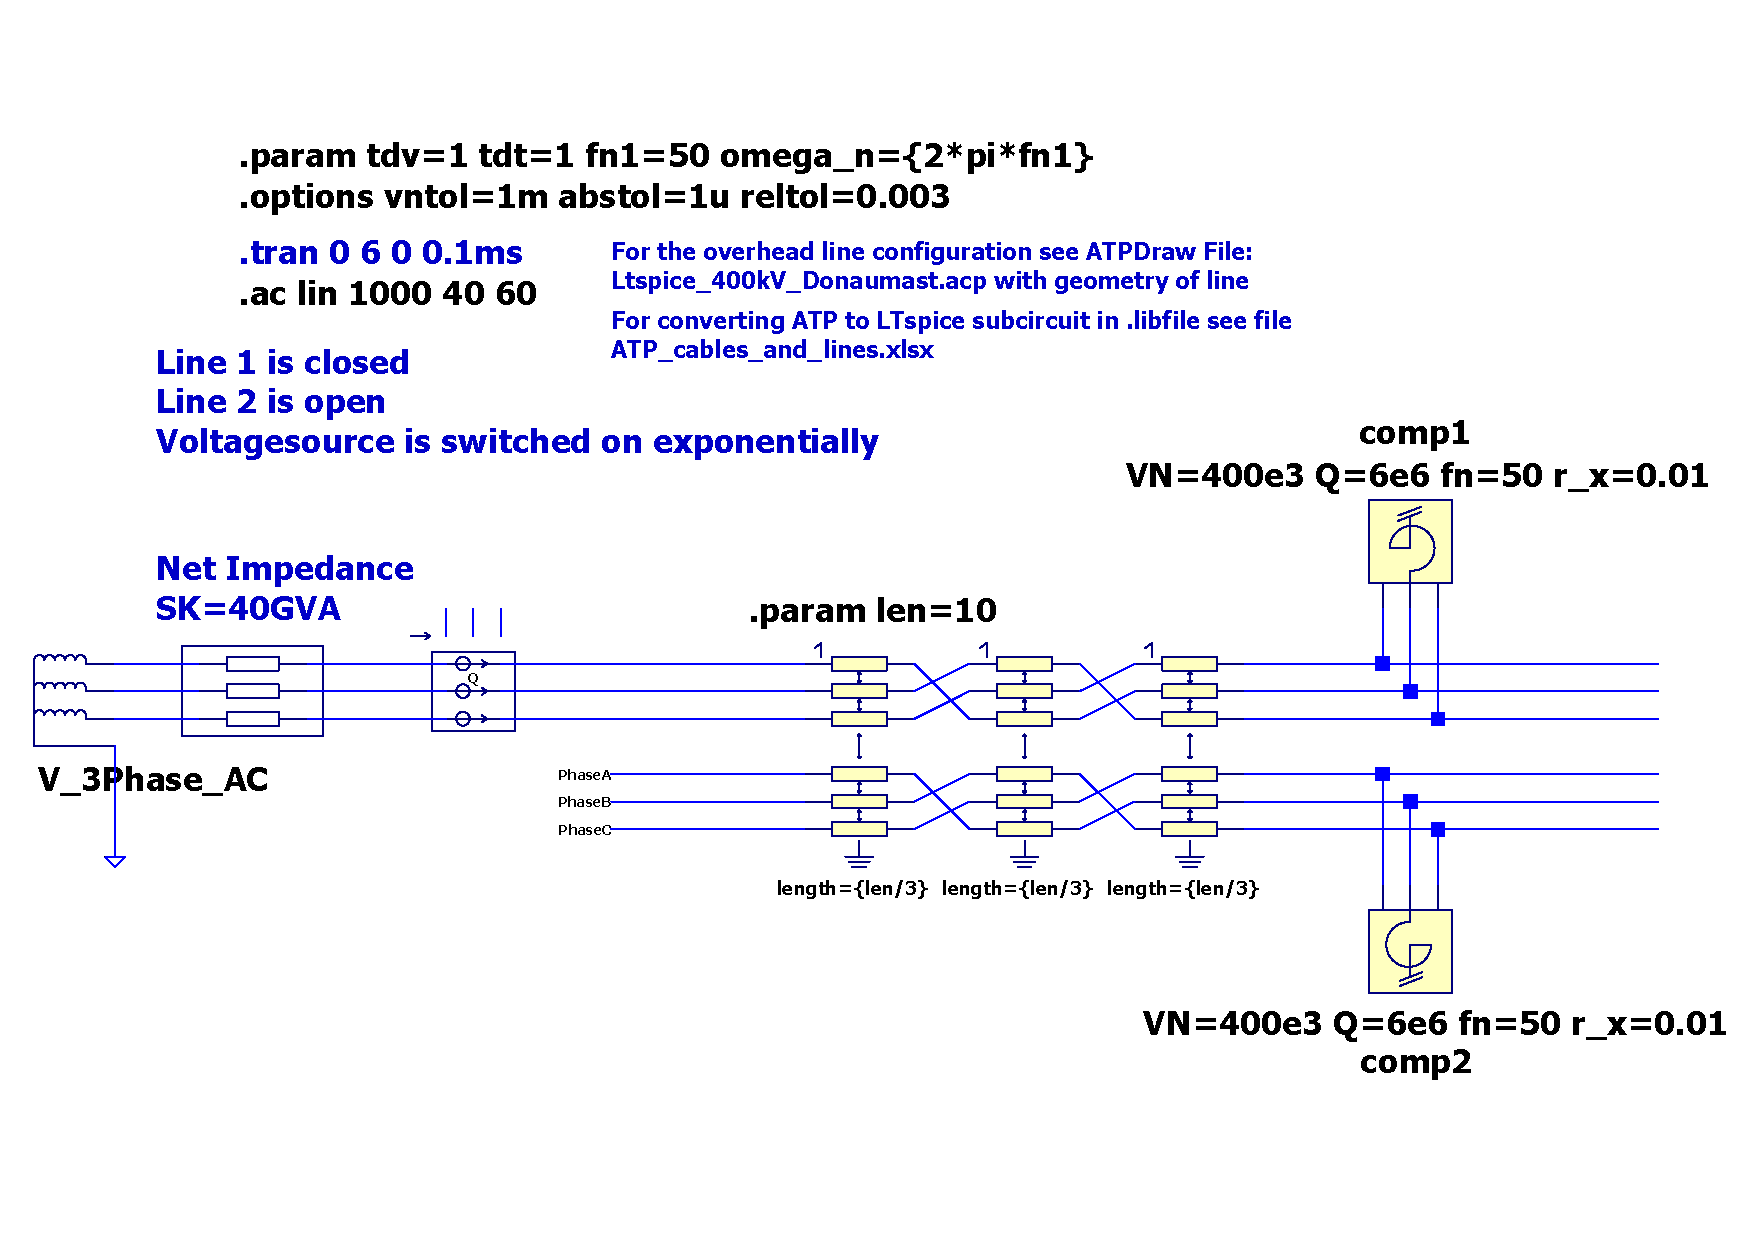
\includegraphics[width=1.0\textwidth]{figures/07_Coupled_lines_resonance/Coupled_lines_resonance_AC_transposed_schematic}
	\caption{Coupled lines resonance schematic Lines2 is open transposed}
	\label{fig:figure78}
\end{figure}

\begin{figure}[H]
	\centering
	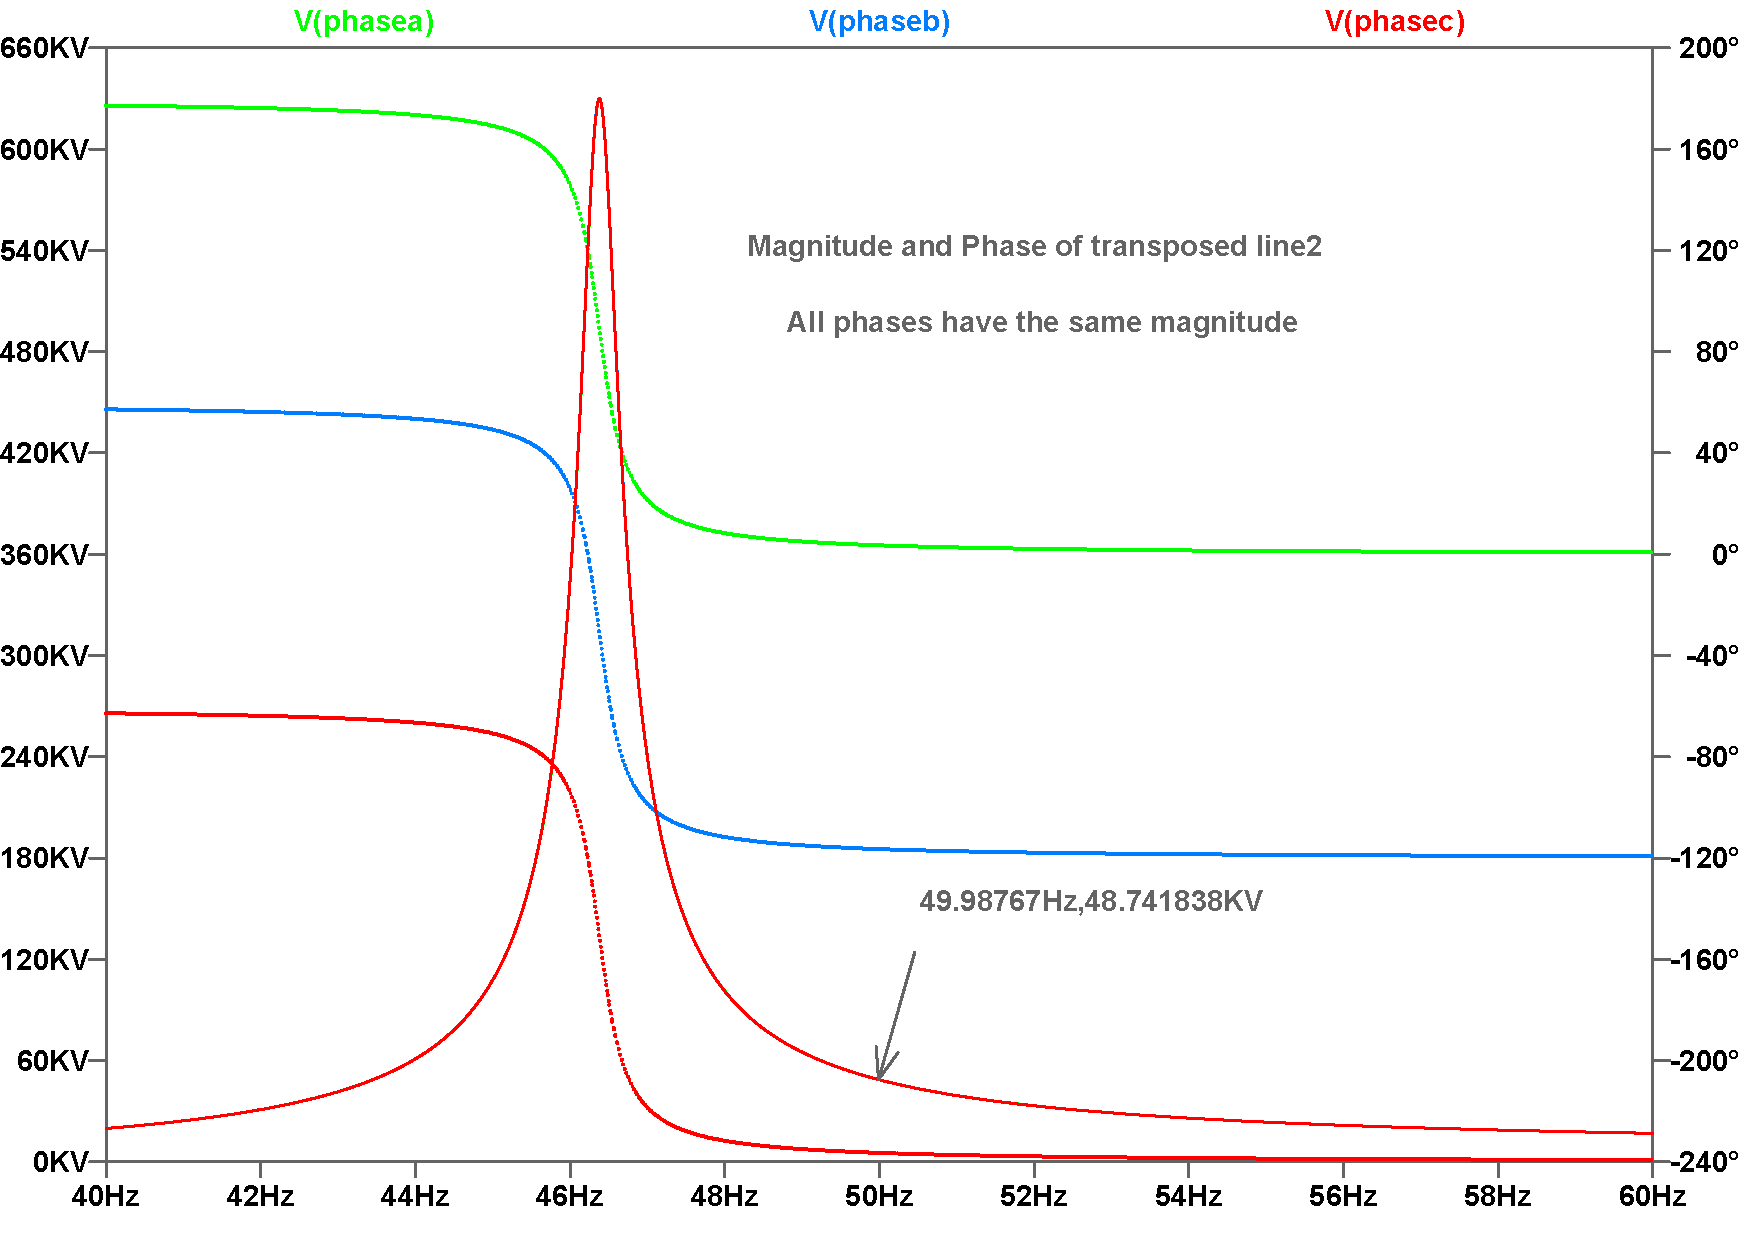
\includegraphics[width=0.90\textwidth]{figures/07_Coupled_lines_resonance/Coupled_lines_resonance_AC_transposed}
	\caption{Coupled lines resonance AC - Lines2 is open transposed}
	\label{fig:figure79}
\end{figure}



\begin{figure}[H]
	\centering
	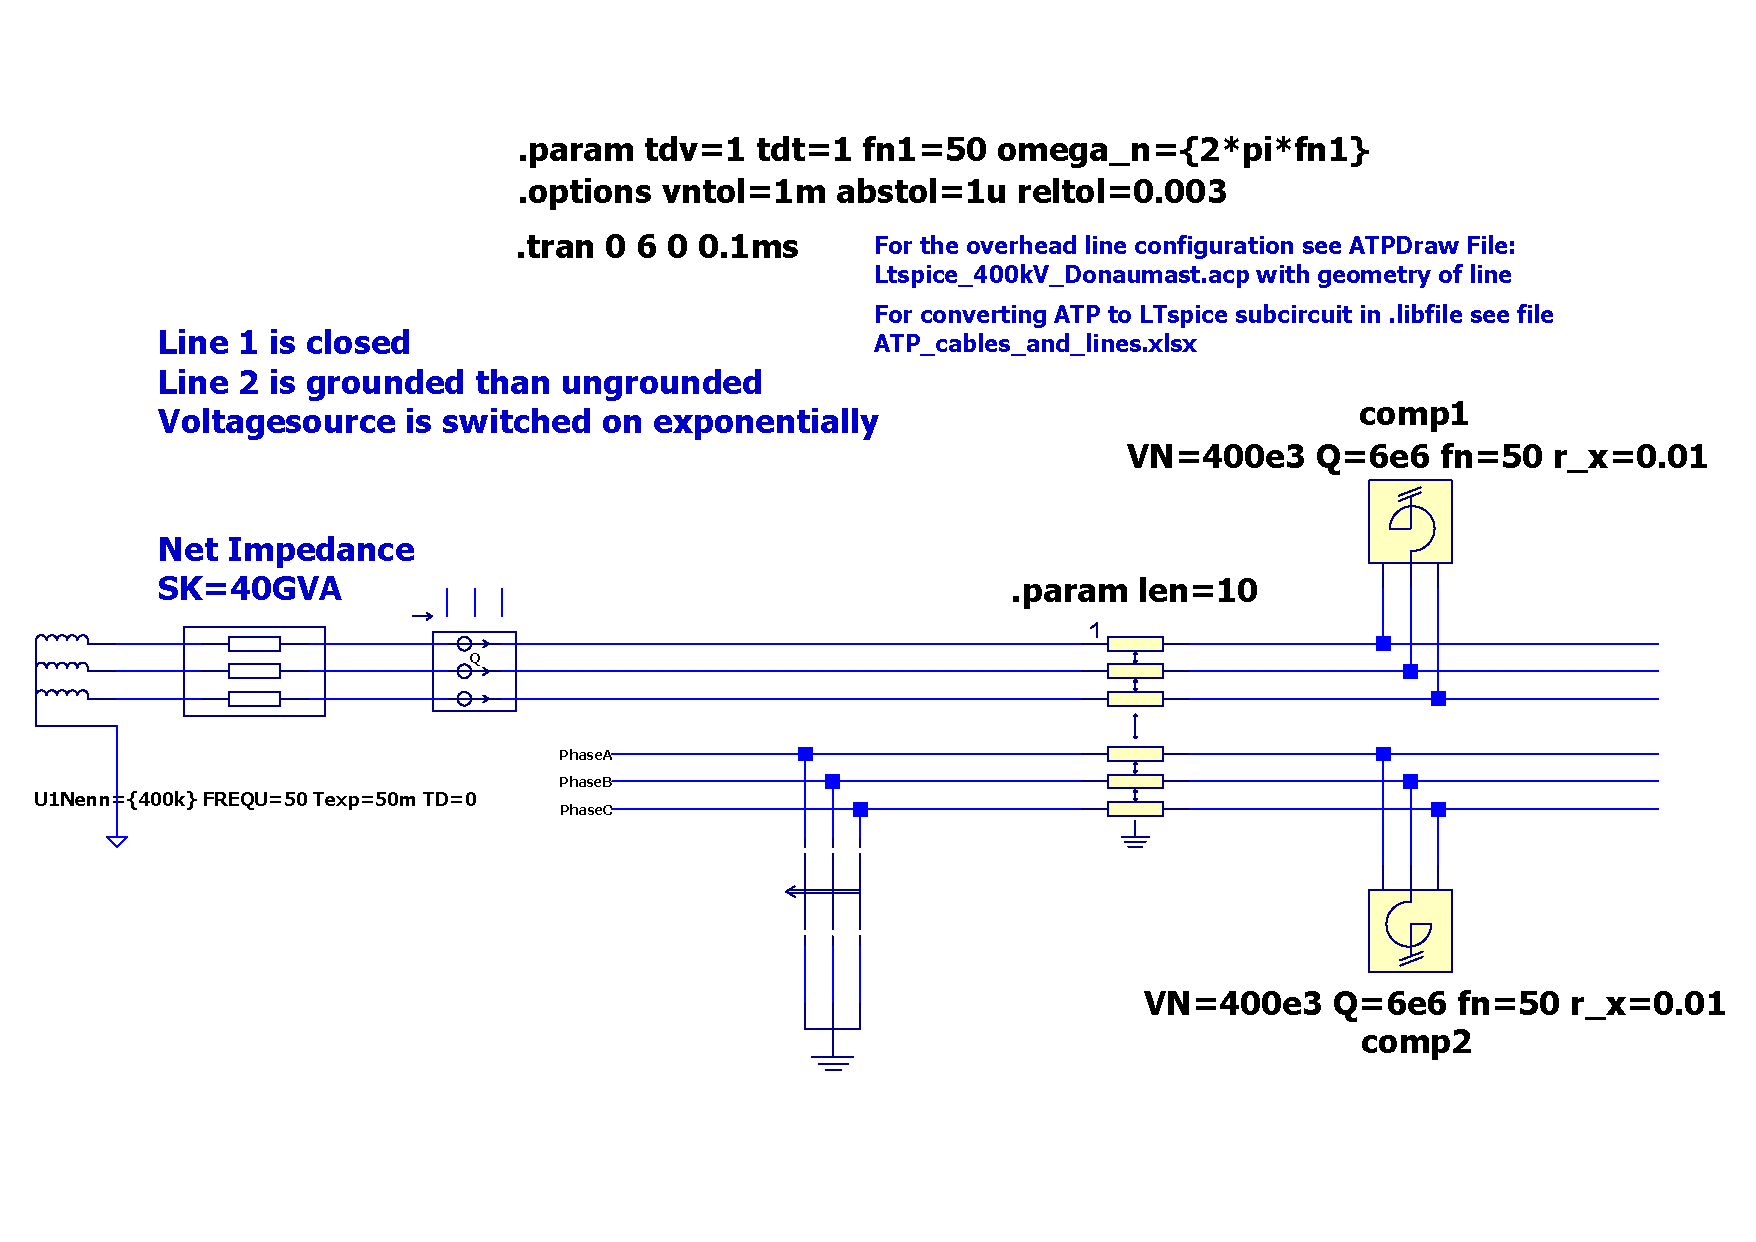
\includegraphics[width=1.0\textwidth]{figures/07_Coupled_lines_resonance/Coupled_lines_resonance_TRAN_grounded_ungrounded_schematic}e
	\caption{Coupled lines resonance TRAN line2 grounded then ungrounded}
	\label{fig:figure710}
\end{figure}

\begin{figure}[H]
	\centering
	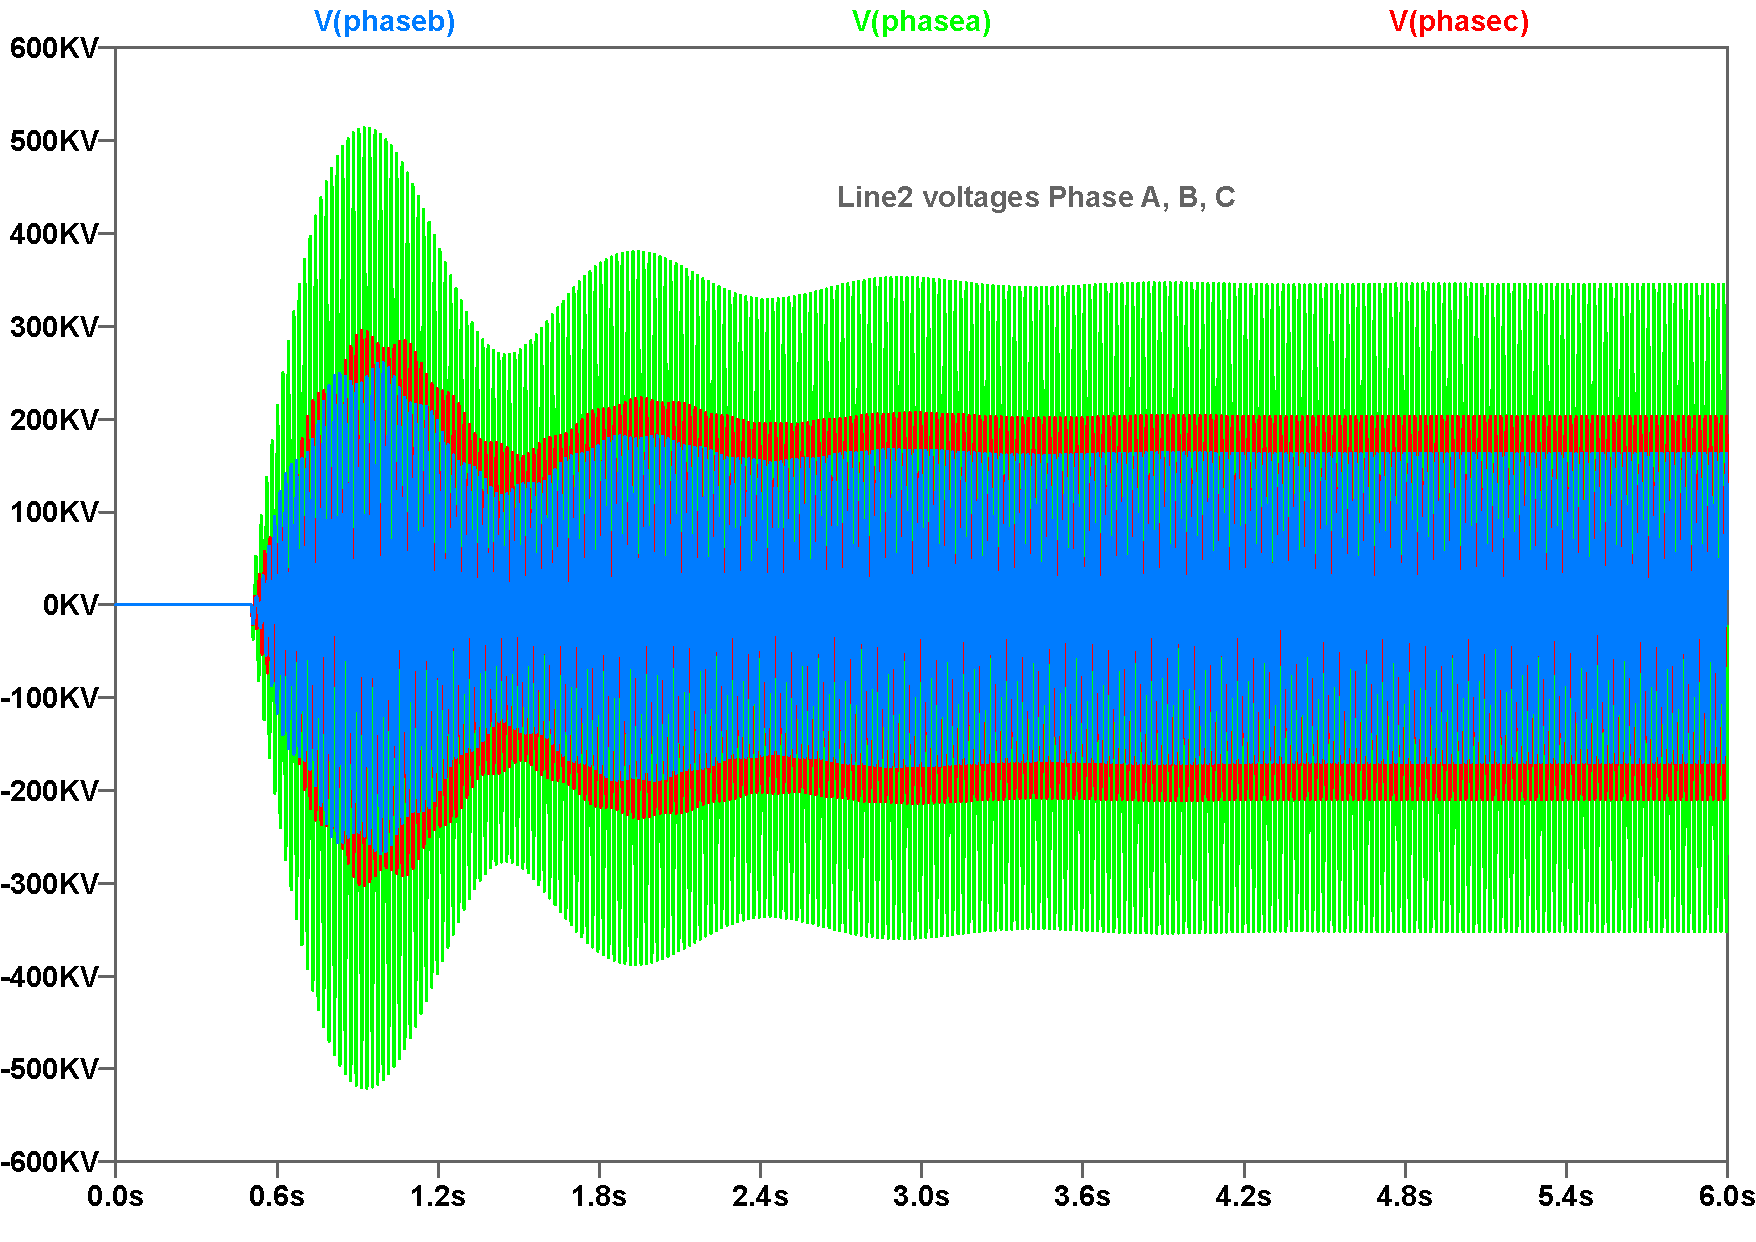
\includegraphics[width=0.90\textwidth]{figures/07_Coupled_lines_resonance/Coupled_lines_resonance_TRAN_grounded_ungrounded}
	\caption{Coupled lines resonance TRAN line2 grounded then ungrounded}
	\label{fig:figure711}
\end{figure}

\section{Line 2 Energized and Subsequently Switched Off} figures: \ref{fig:figure712}-\ref{fig:figure713} (simulation-file: same name as the heading)
\label{sec:coupled-line-switched-off}

Line 2 is disconnected at \SI{500}{\milli\second}. Immediately after opening, its voltage swings to
approximately \SI{-430}{\kilo\volt}. Phase R shows a long-period beat, while
phases B and C show a shorter-period envelope associated with the
\SI{44}{\hertz} resonance.

Select the Phase C voltage and draw a zoom window between two adjacent envelope
maxima. The LTspice status line indicates approximately \SI{5.7}{\hertz}. This
is close to the difference between the source frequency and the second natural
frequency:

\begin{equation}
f_{\mathrm{beat}}\approx
 \left|f_{\mathrm s}-f_{\mathrm r,2}\right|
 \approx\left|\SI{50}{\hertz}-\SI{44}{\hertz}\right|
 \approx\SI{6}{\hertz}.
\end{equation}

\begin{remark}{Exercise}{imp:coupled-line-opening-time}
Save the model as \texttt{test.asc}, change the opening time to
\SI{0.510}{\second}, and compare the phase-voltage peaks. The trapped initial
conditions at the switching instant strongly influence the subsequent free
oscillation.
\end{remark}

\section{Line 2 Switched Off Without a Shunt-Reactor} figures: \ref{fig:figure714}-\ref{fig:figure715}  (simulation-file: same name as the heading)
\label{sec:coupled-line-open-without-reactor}

After line 2 is switched off, its induced phase-voltage peaks are only approximately
\SIrange{20}{30}{\kilo\volt}. Without the \texttt{l\_batt} element, the
near-power-frequency resonance is absent. 

\begin{figure}[H]
	\centering
	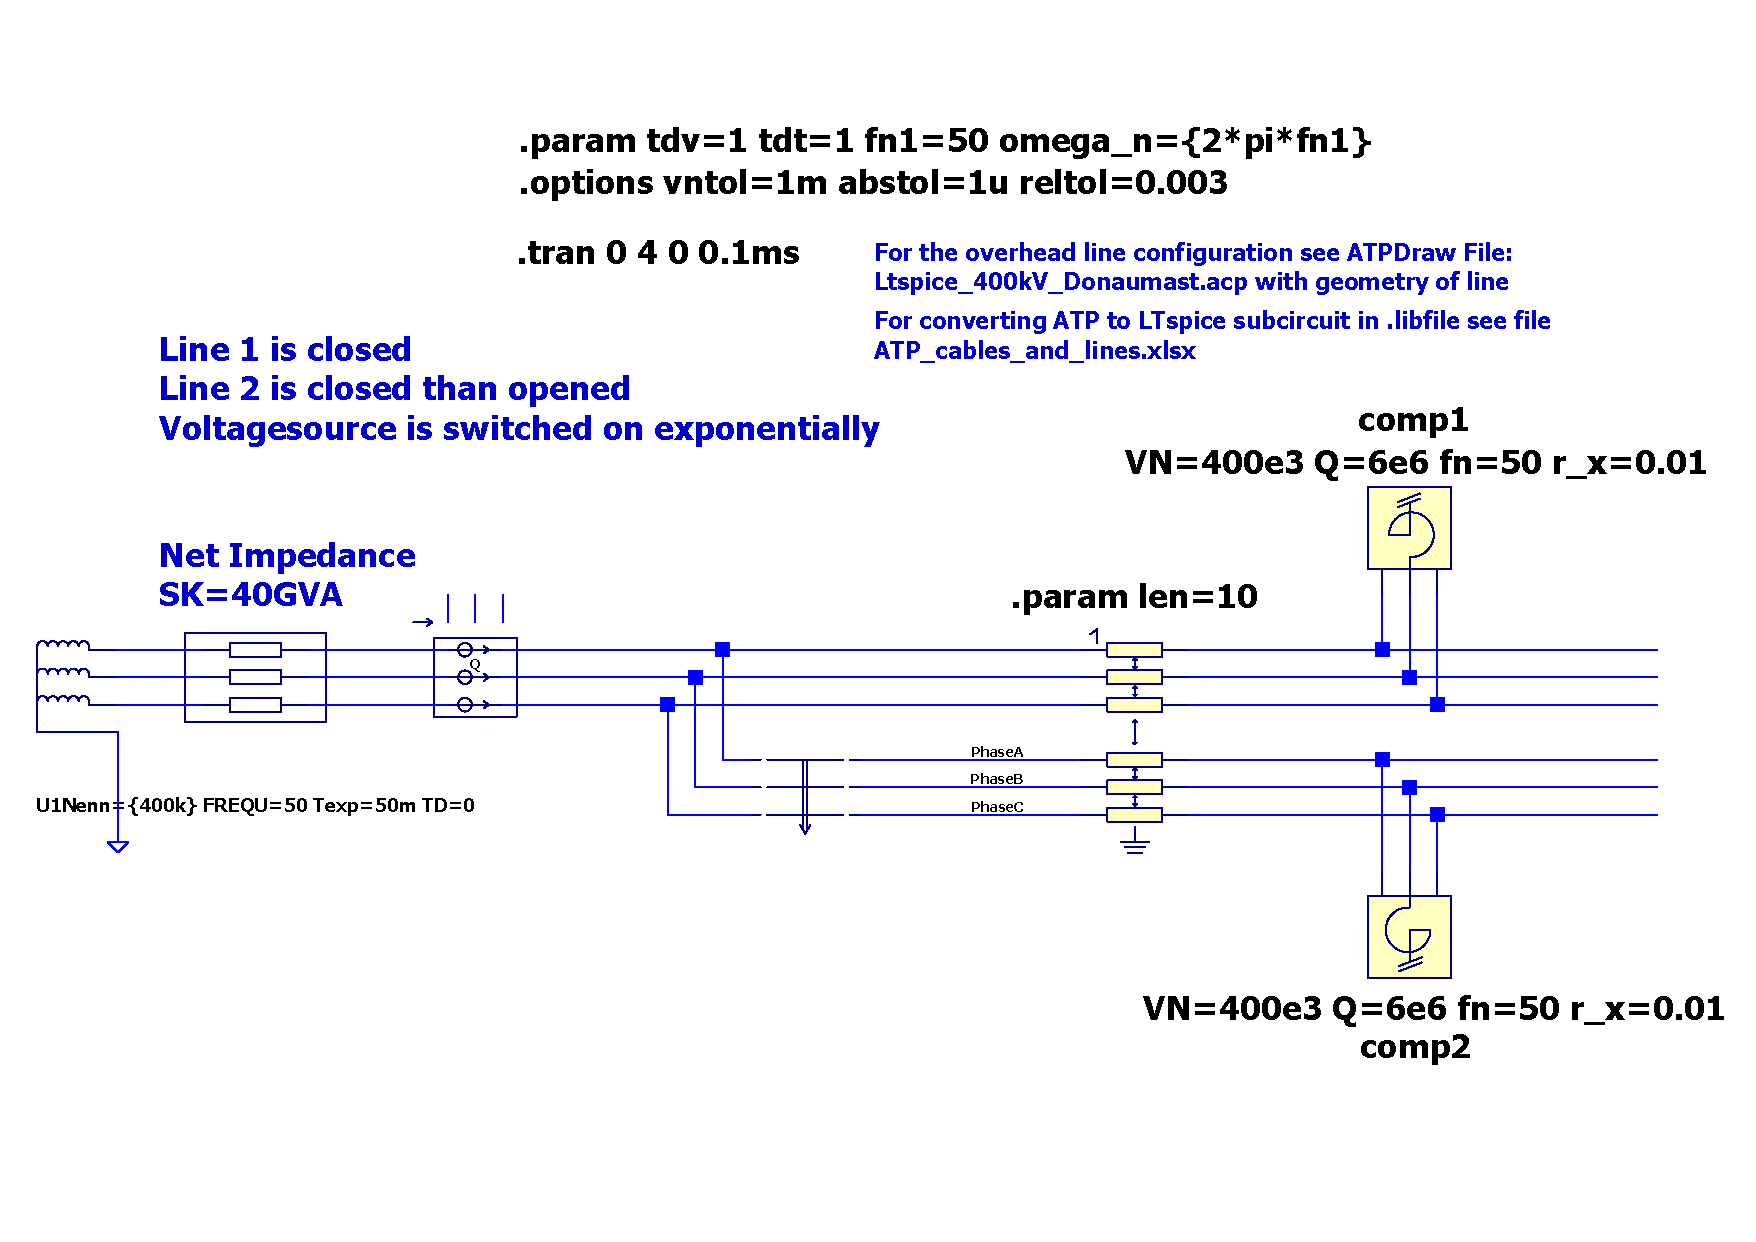
\includegraphics[width=1.0\textwidth]{figures/07_Coupled_lines_resonance/Coupled_lines_resonance_TRAN_switched_off_schematic}
	\caption{Coupled lines resonance TRAN line2 switched off  schematic}
	\label{fig:figure712}
\end{figure}

\begin{figure}[H]
	\centering
	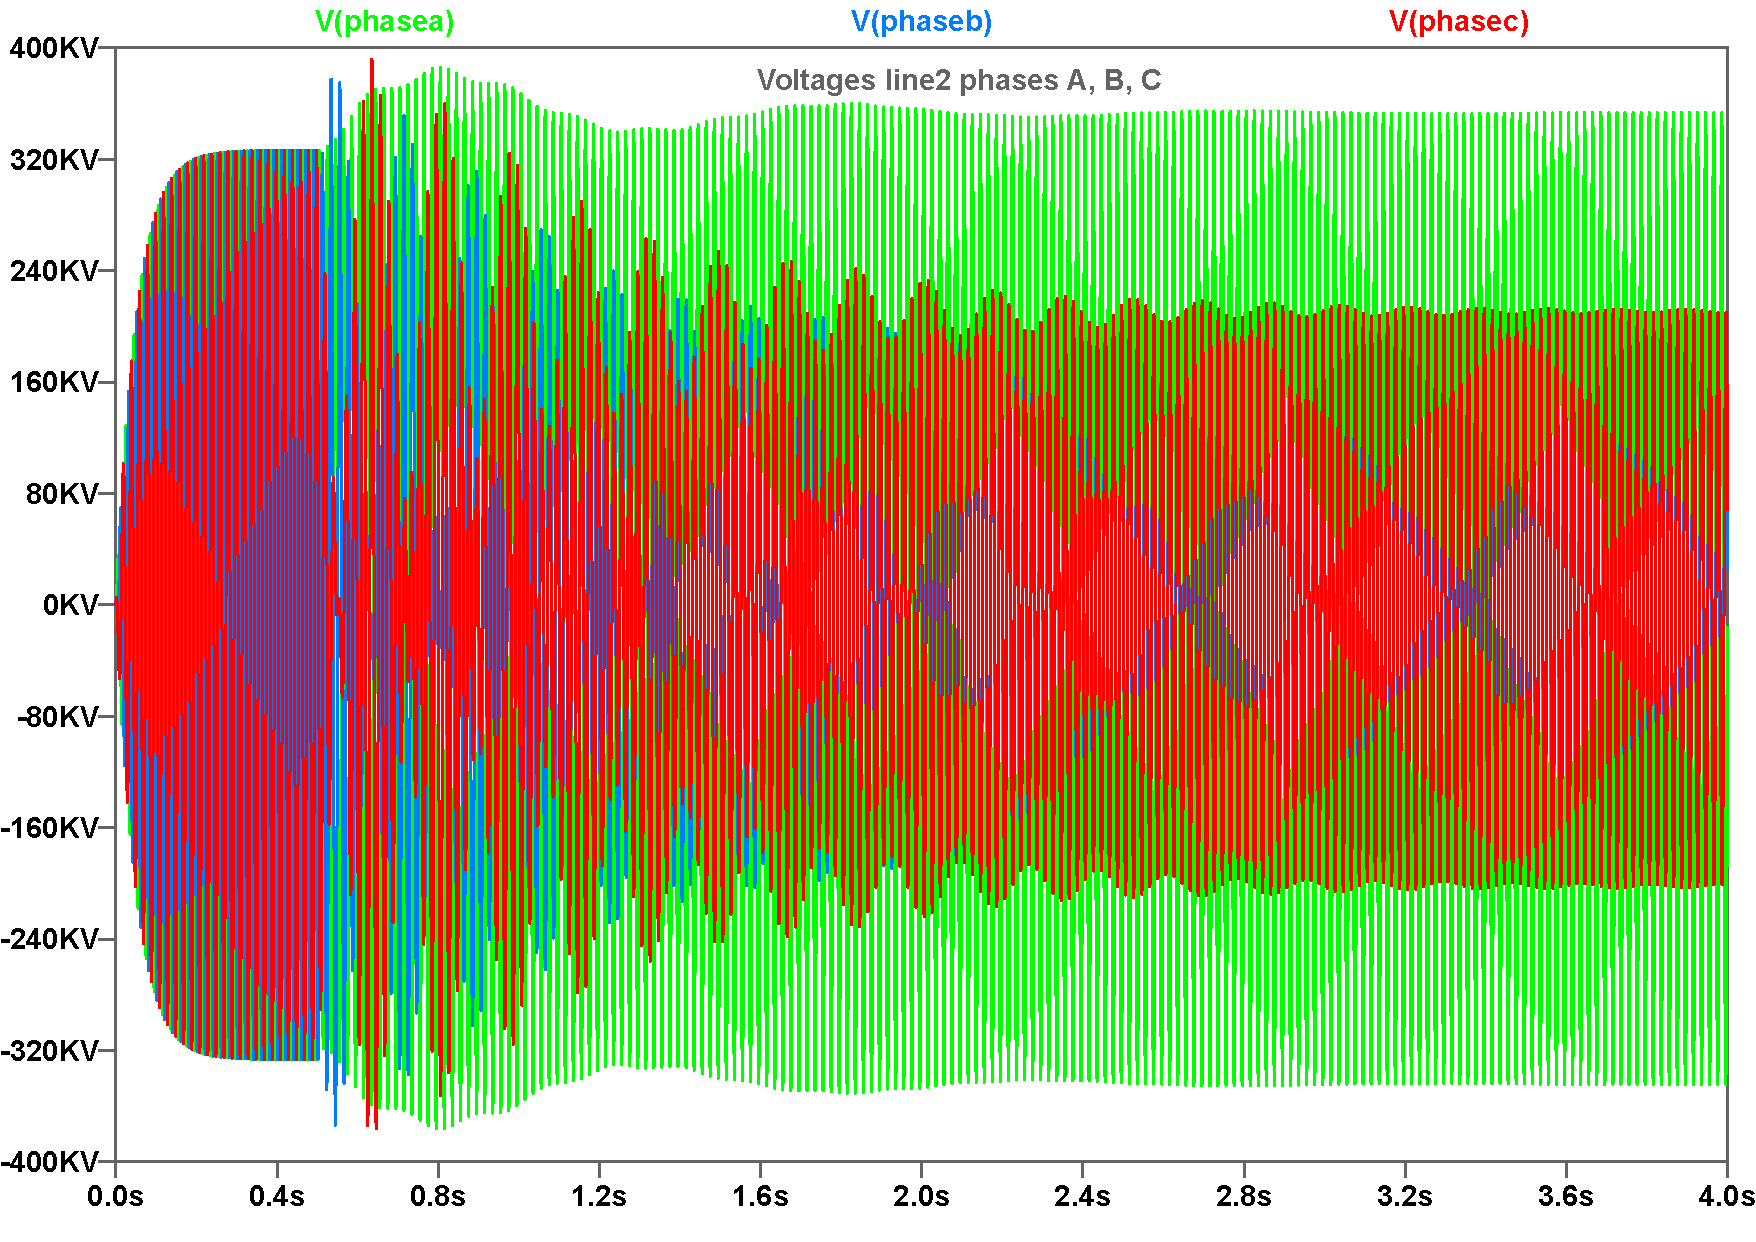
\includegraphics[width=0.90\textwidth]{figures/07_Coupled_lines_resonance/Coupled_lines_resonance_TRAN_switched_off}
	\caption{Coupled lines resonance TRAN line2 switched off}
	\label{fig:figure713}
\end{figure}

\begin{figure}[H]
	\centering
	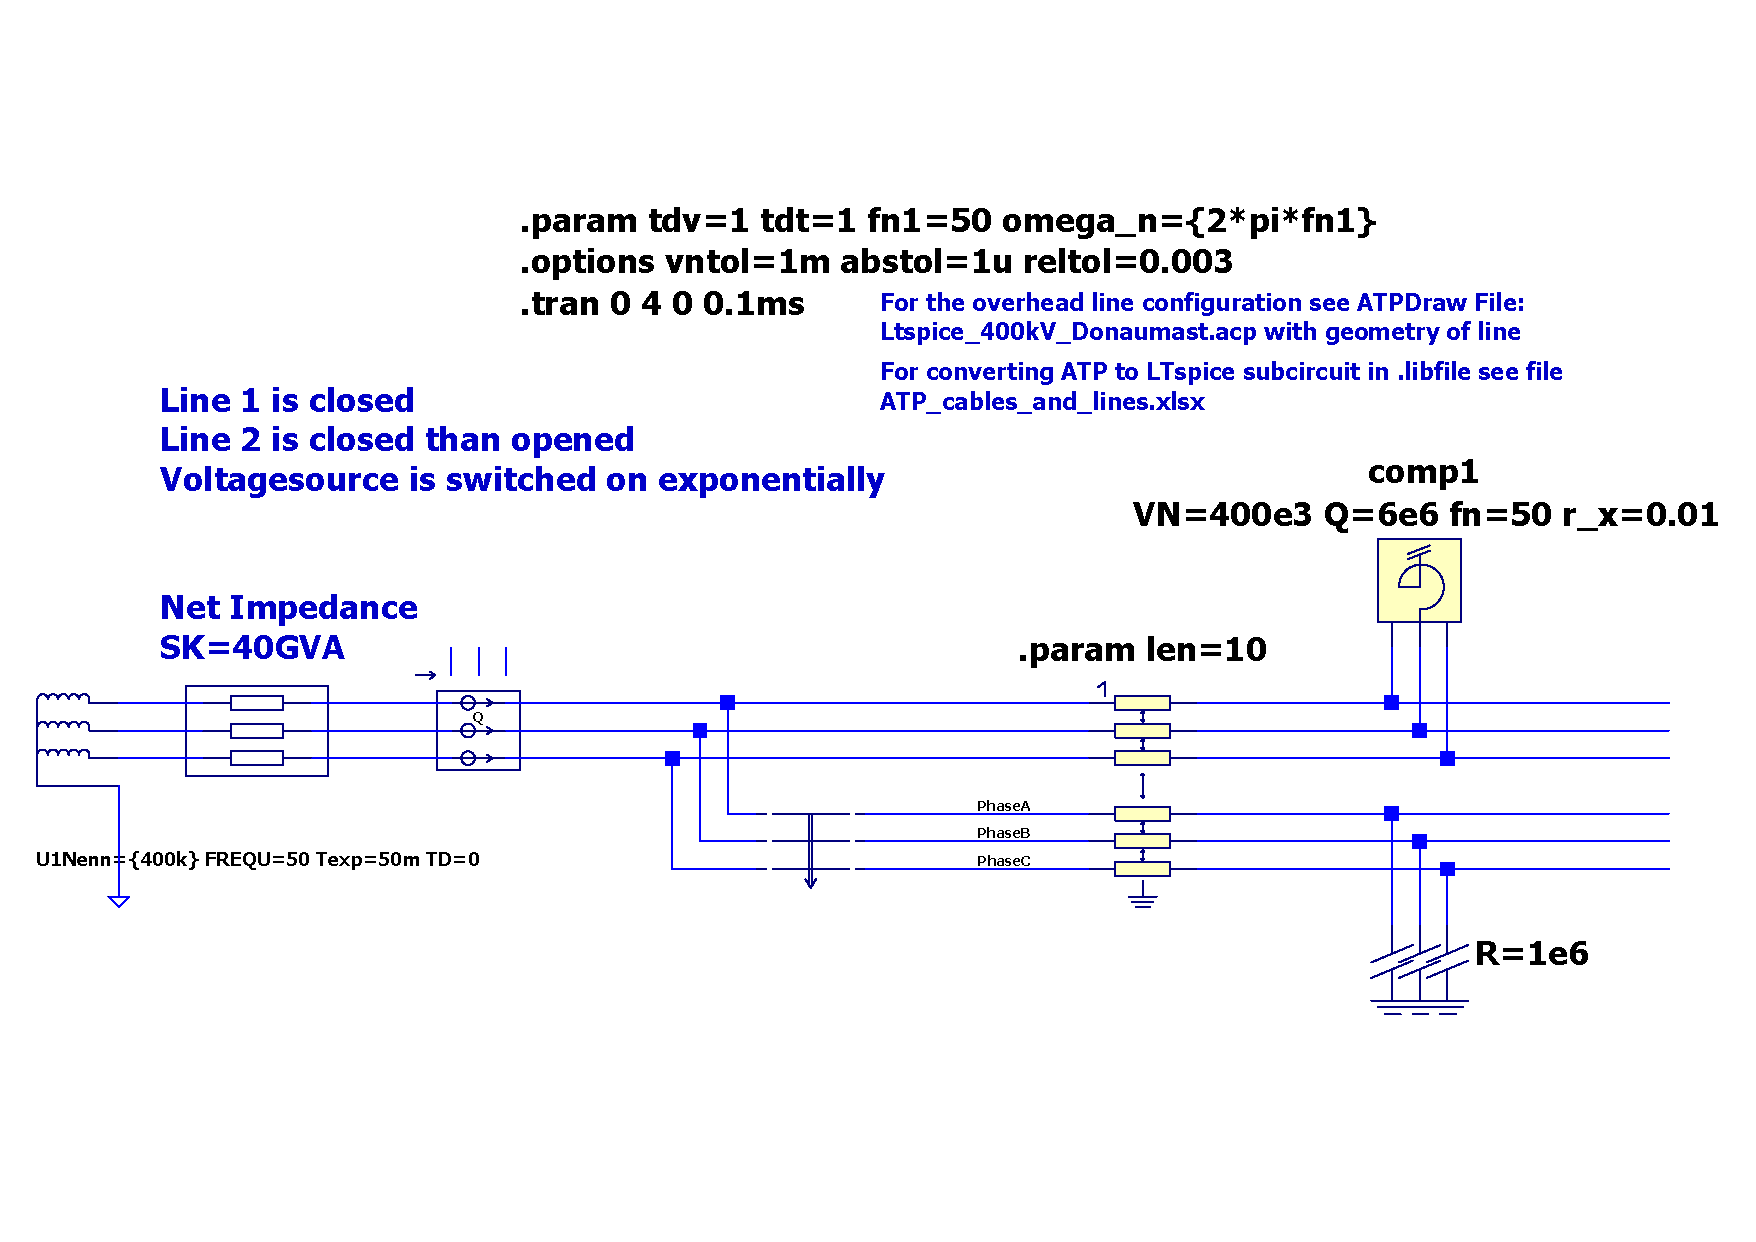
\includegraphics[width=1.0\textwidth]{figures/07_Coupled_lines_resonance/Coupled_lines_resonance_TRAN_switched_off_wo_shuntreactor_schematic}
	\caption{Coupled lines resonance TRAN line2 switched off without shunt reactor schematic }
	\label{fig:figure714}
\end{figure}

\begin{figure}[H]
	\centering
	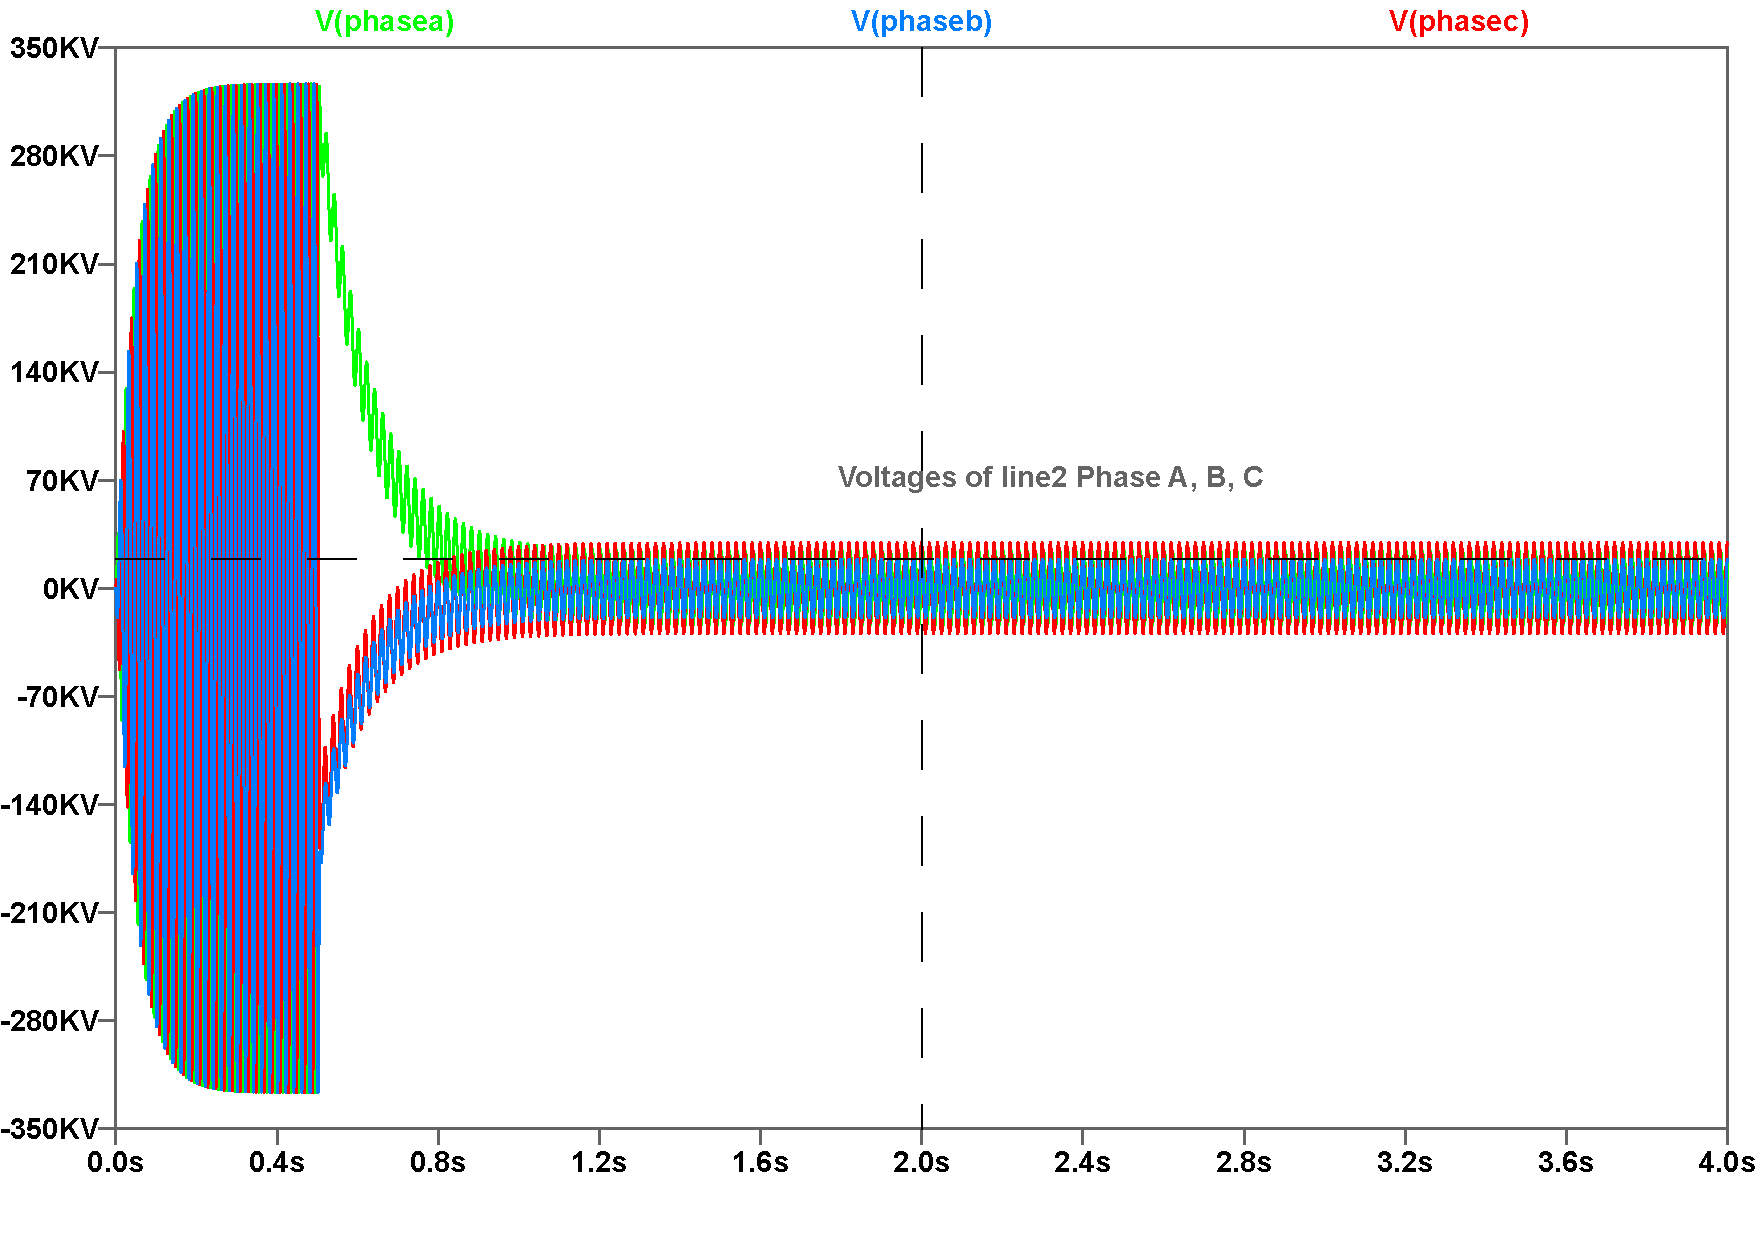
\includegraphics[width=0.90\textwidth]{figures/07_Coupled_lines_resonance/Coupled_lines_resonance_TRAN_switched_off_wo_shuntreactor}
	\caption{Coupled lines resonance TRAN line2 switched off without shunt reactor}
	\label{fig:figure715}
\end{figure}

\section{Stored Energy on the Open Line} figure: 7.16 717 (simulation-file: same name as the heading)
\label{sec:coupled-line-stored-energy}

Line 1 is initially energized and then disconnected. Line 2 is subsequently grounded. To measure
the dissipated energy, hold \textsc{Alt} and click the grounding element, then
hold \textsc{Ctrl} and click the generated power trace. LTspice integrates the
power and displays the corresponding energy. 
NOTE: In this case, the energy should be measured from 1 s to 2 s. Zoom into or set the x-axis to the interval from 1 s to 2 s. During this interval, the stored energy decreases substantially after the line is switched off
After two seconds, only the energy transfer from Line 1 to Line 2 via capacitive coupling between both lines remains. 
This (small) energy should not be included in the measurement.     

The energy released from line 2 is approximately \SI{2.2}{\kilo\joule}.
The stored energy is therefore comparatively small.
With a grounding resistance of \SI{100}{\ohm}, the open-line voltage collapses
almost immediately. It also collapses with \SI{10}{\kilo\ohm}, showing that
the mutual coupling path to line 1 is relatively high-impedance at
\SI{50}{\hertz}.

\begin{figure}[H]
	\centering
	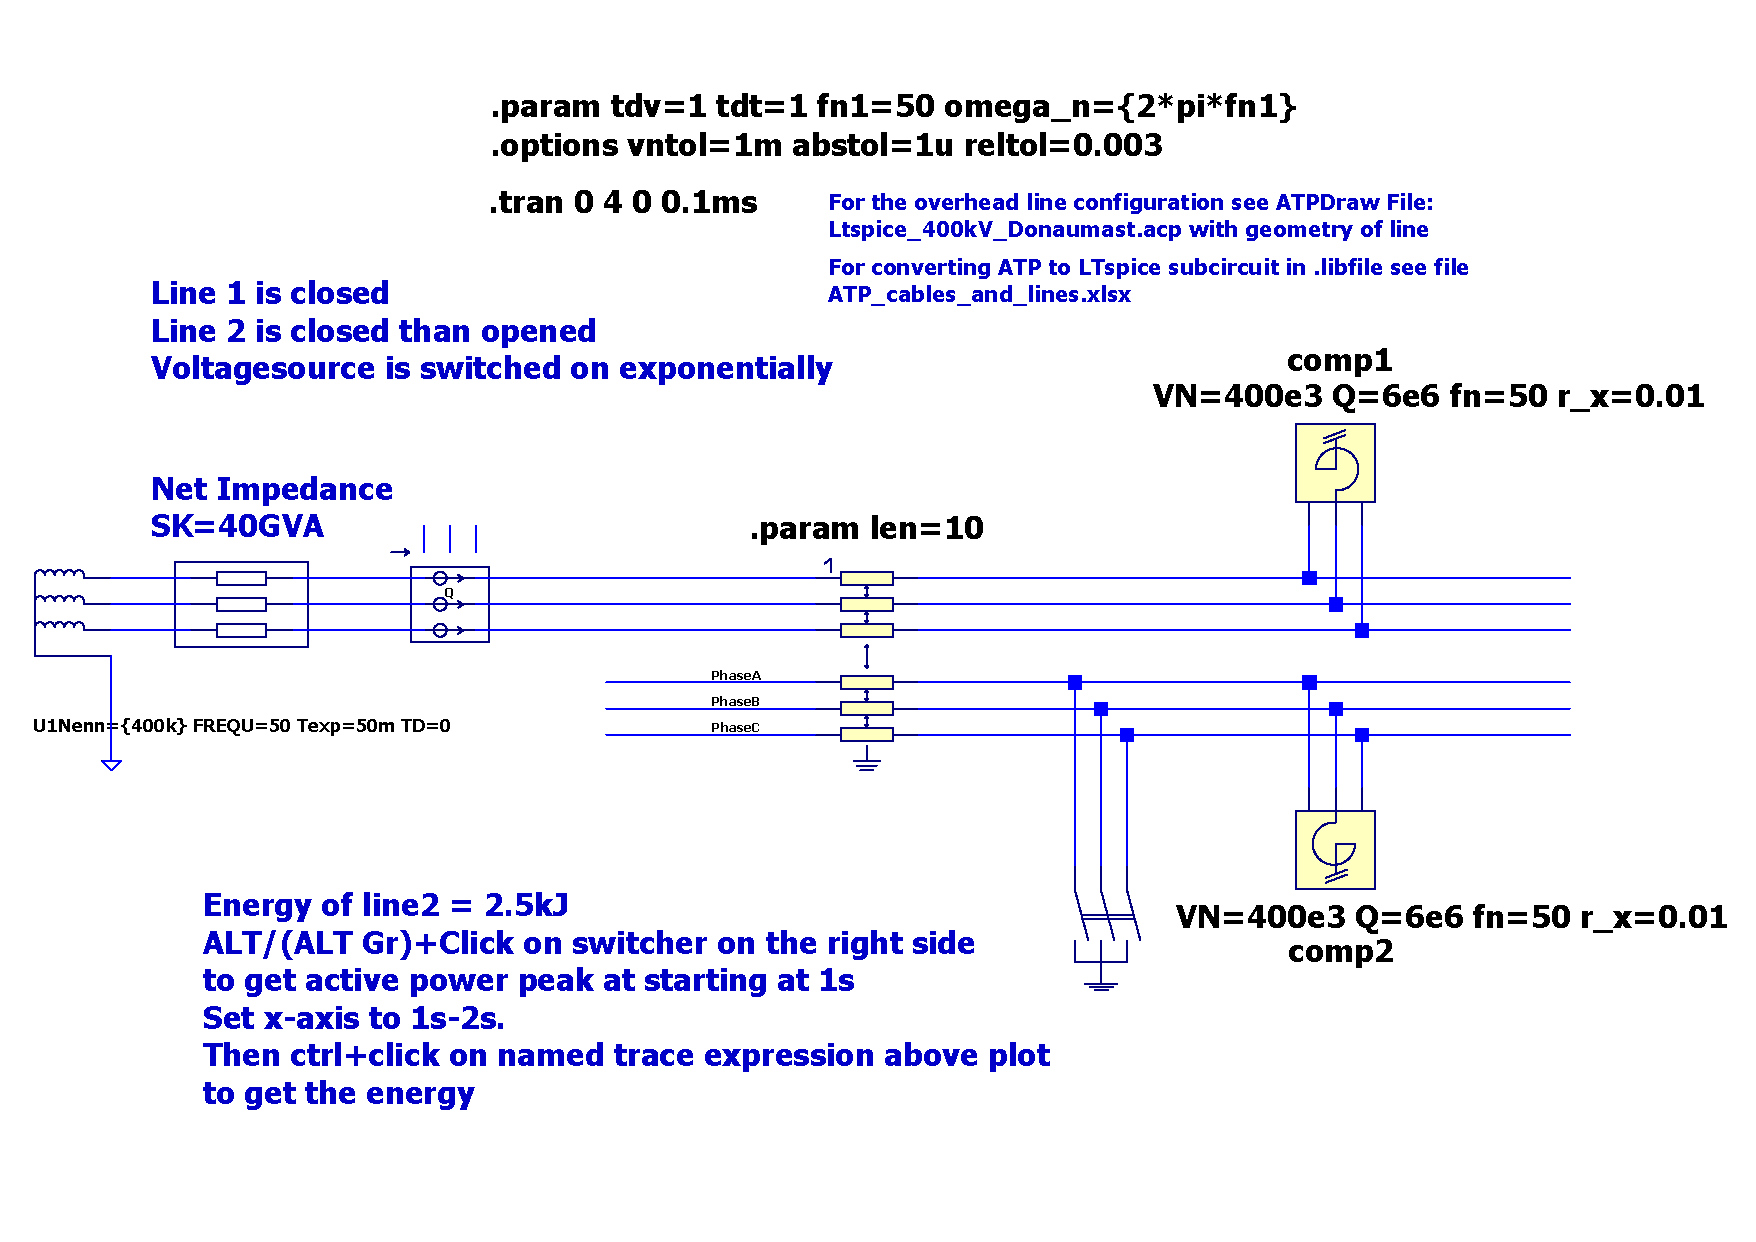
\includegraphics[width=1.0\textwidth]{figures/07_Coupled_lines_resonance/Coupled_lines_resonance_TRAN_stored_energy_schematic}
	\caption{Coupled lines resonance TRAN line2 stored energy schematic }
	\label{fig:figure716}
\end{figure}

\begin{figure}[H]
	\centering
	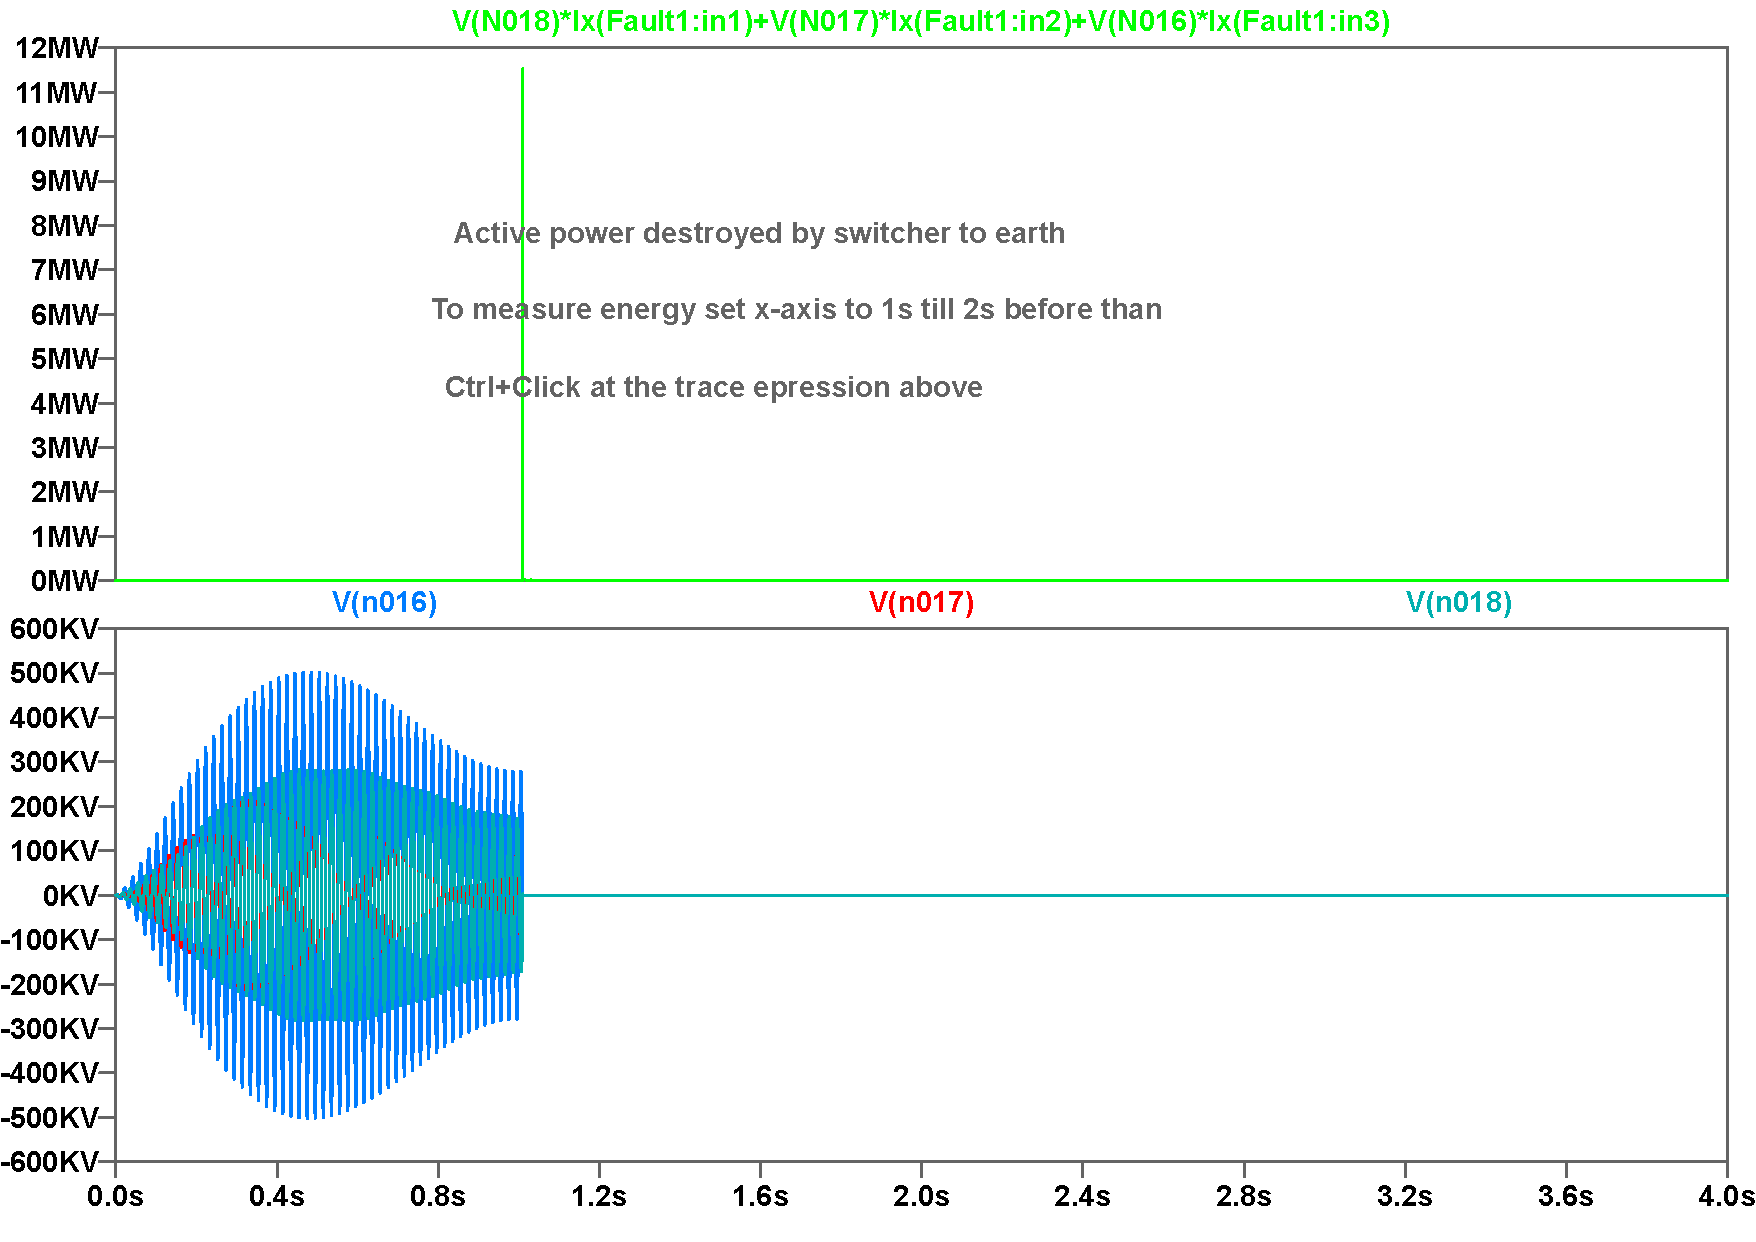
\includegraphics[width=0.90\textwidth]{figures/07_Coupled_lines_resonance/Coupled_lines_resonance_TRAN_stored_energy}
	\caption{Coupled lines resonance TRAN line2 stored energy}
	\label{fig:figure717}
\end{figure}


\begin{chaptersummary}
Mutual inductive and capacitive coupling can impose substantial voltages on an
open overhead-line circuit. Near-exact shunt compensation may place a natural
frequency close to \SI{50}{\hertz} and amplify the open-line voltage to a
dangerous level. Phase transposition symmetrizes the coupling and, in this
example, shifts the resonance away from the operating frequency. Removing the
compensation reactor eliminates the near-power-frequency resonance, while its
loss parameter controls damping.
\end{chaptersummary}

% ============================================================
% Synchronous generator operating modes
% Content file for the Power System Simulation with LTspice book.
% All formatting is provided by the central preamble.tex.
% ============================================================

\chapter{Operating Modes of Synchronous Generators}
\label{chap:synchronous-generator-operating-modes}
\index{synchronous generator!operating modes}
\index{synchronous generator!island operation}
\index{synchronous generator!grid-connected operation}
\index{synchronous generator!constant-speed operation}

This chapter demonstrates three important operating modes of a synchronous
generator:

\begin{itemize}
  \item isolated or island operation,
  \item operation connected to a stiff power network, and
  \item operation at fixed mechanical speed.
\end{itemize}

The examples illustrate voltage and speed control, synchronization, active-
and reactive-power control, load-angle stability, and the behaviour of the
machine during symmetrical and asymmetrical faults.

% ============================================================
\section{Isolated Operation}
\label{sec:sg-isolated-operation}
% ============================================================

\subsection{General}

In isolated operation, no external voltage source maintains the network
voltage or frequency. An automatic voltage regulator (AVR) is therefore
required to regulate the terminal voltage, while a speed governor must balance
the mechanical input power against the electrical load. The example also
demonstrates how a second synchronous generator can be synchronized with the
island network.

Adding generators can increase the total inertia and improve the response of
the island system. Stable load sharing, however, requires suitable governor
and excitation-control characteristics.

\begin{important}{Control requirements in island operation}{imp:island-control}
An island network requires at least one unit that regulates frequency and at
least one unit that regulates voltage. In practical parallel operation,
governor droop and AVR reactive-power or voltage droop are normally used to
share active and reactive power between the generators.
\end{important}

\subsection{Circuit Design}

The circuit \texttt{Simulation\_Start} contains a round-rotor synchronous generator rated at
\SI{400}{\mega\watt} and \SI{20}{\kilo\volt}. It is connected through a
transformer rated at \SI{20}{\kilo\volt} on the generator side and
\SI{400}{\kilo\volt} on the network side. A switch connects the generator
to the initially unloaded network at \SI{1}{\second}.
The load increases linearly from zero to \SI{50}{\mega\watt} between
\SI{2}{\second} and \SI{5}{\second}. The AVR is enabled at
\SI{6}{\second}, whereas the speed governor remains active throughout the
simulation. During the first second, the main field winding is supplied by a
temporary excitation ramp from \SI{600}{\volt} to \SI{1400}{\volt} and
back to \SI{600}{\volt}. This accelerates the buildup of the rated terminal
voltage.
The AVR measures the voltage on the high-voltage side and uses a reference of
\SI{400}{\kilo\volt}. The governor reference is
\SI{1500}{\rpm}. Its switching time is placed outside the simulated interval,
for example at \SI{500}{\second}, so that the controller remains active.
Both external controllers are implemented as simple PI controllers to
illustrate the fundamental behaviour of the controlled machine. Their dynamics
are intentionally fast in order to shorten the simulation.

\begin{simulation}{AVR switching sequence}{sim:island-avr-switching}
The AVR switch must close shortly before the switch supplying the fixed field
voltage opens. The field voltage must not be interrupted, because this would
cause the terminal voltage to collapse. Since the excitation circuit may carry
a high current, the switch on-resistance must be sufficiently small to avoid an
unwanted field-voltage drop.

The torque-control changeover is less critical. Owing to the large moment of
inertia $J$, the rotor speed cannot change abruptly even if the electromagnetic
or mechanical torque is briefly disturbed.
\end{simulation}

\subsection{Simulation Start} see Figures: \ref{fig:figure81} and \ref{fig:figure82}  (simulation-file: same name as the heading)

The machine starts with zero terminal voltage. The initial field-voltage boost
to \SI{1400}{\volt} allows the rated voltage to be reached quickly. For this
demonstration, the stator copper-resistance parameter \texttt{Rcu} is set to
\num{0.01} to accelerate voltage buildup and thereby reduce simulation time.

\subsection{Voltage Behaviour} see Figures: \ref{fig:figure81} and \ref{fig:figure82}

After approximately \SI{1}{\second}, the network voltage reaches
\SI{400}{\kilo\volt}, corresponding to \SI{20}{\kilo\volt} at the
generator terminals. As the load rises from zero to
\SI{50}{\mega\watt}, the network voltage falls slightly to approximately
\SI{397}{\kilo\volt}. When the AVR is enabled at \SI{6}{\second}, it
rapidly restores the voltage to \SI{400}{\kilo\volt}.

In an island network, a voltage change can also change the active and reactive
power absorbed by voltage-dependent loads. For an ideal constant-power load,
by contrast, the specified active and reactive powers remain constant and the
current changes as the voltage changes.

\subsection{Speed Behaviour} see Figures: \ref{fig:figure81} and \ref{fig:figure82}

During the load ramp, the speed initially falls below \SI{1500}{\rpm}. Once
the final load has been reached and the governor has increased the mechanical
torque, the speed returns to its reference value. When the AVR is enabled, the
rising voltage temporarily increases the load current and electromagnetic
torque. Consequently, the frequency briefly decreases before returning to its
steady-state value.

\subsection{Load Angle and Load Steps} see Figures: \ref{fig:figure83}-\ref{fig:figure86}  (simulation-file: same names as the heading)

During the first load ramp, the load angle increases and settles at
approximately \ang{12}. A \SI{30}{\mega\watt} load step can be introduced
by setting \texttt{Vfact=3} at \SI{2}{\second} and closing an additional
switch at \SI{3}{\second}. Further load steps at \SI{5}{\second} and
\SI{7}{\second} increase the generator output from
\SI{30}{\mega\watt} to \SI{60}{\mega\watt} and finally to
\SI{90}{\mega\watt}. The maximum load angle is approximately \ang{21}.

Each load step produces a transient change in frequency and load angle. The
governor subsequently establishes a new torque balance.

\begin{figure}[H]
	\centering
	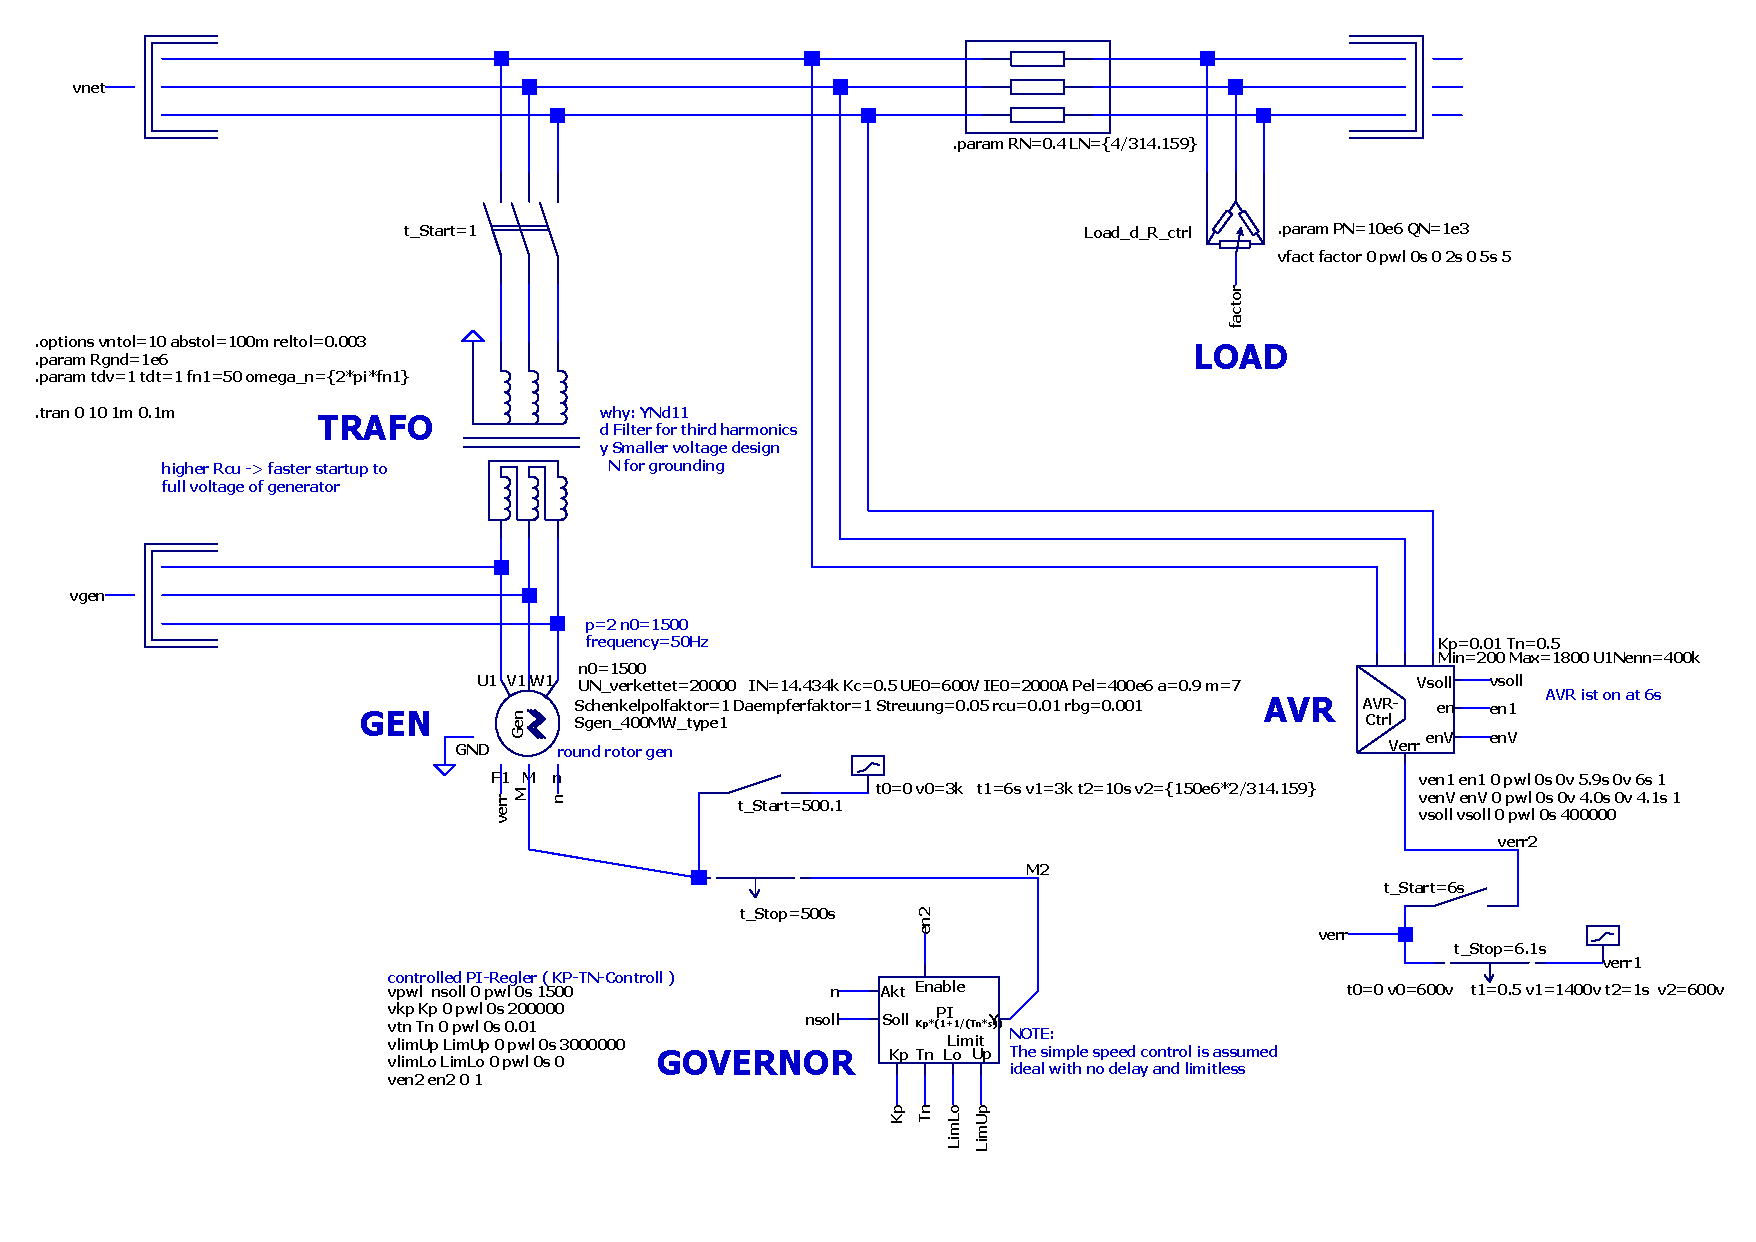
\includegraphics[width=1\textwidth] {figures/08_Synchronous_Generator/Synchronous_Generator_Isolated_mode_500MVA/Simulation_Start_Schematic.pdf}
	\caption{Simulation start - Voltage behaviour - Speed behaviour  - schematic}
	\label{fig:figure81}
\end{figure}

\begin{figure}[H]
	\centering
	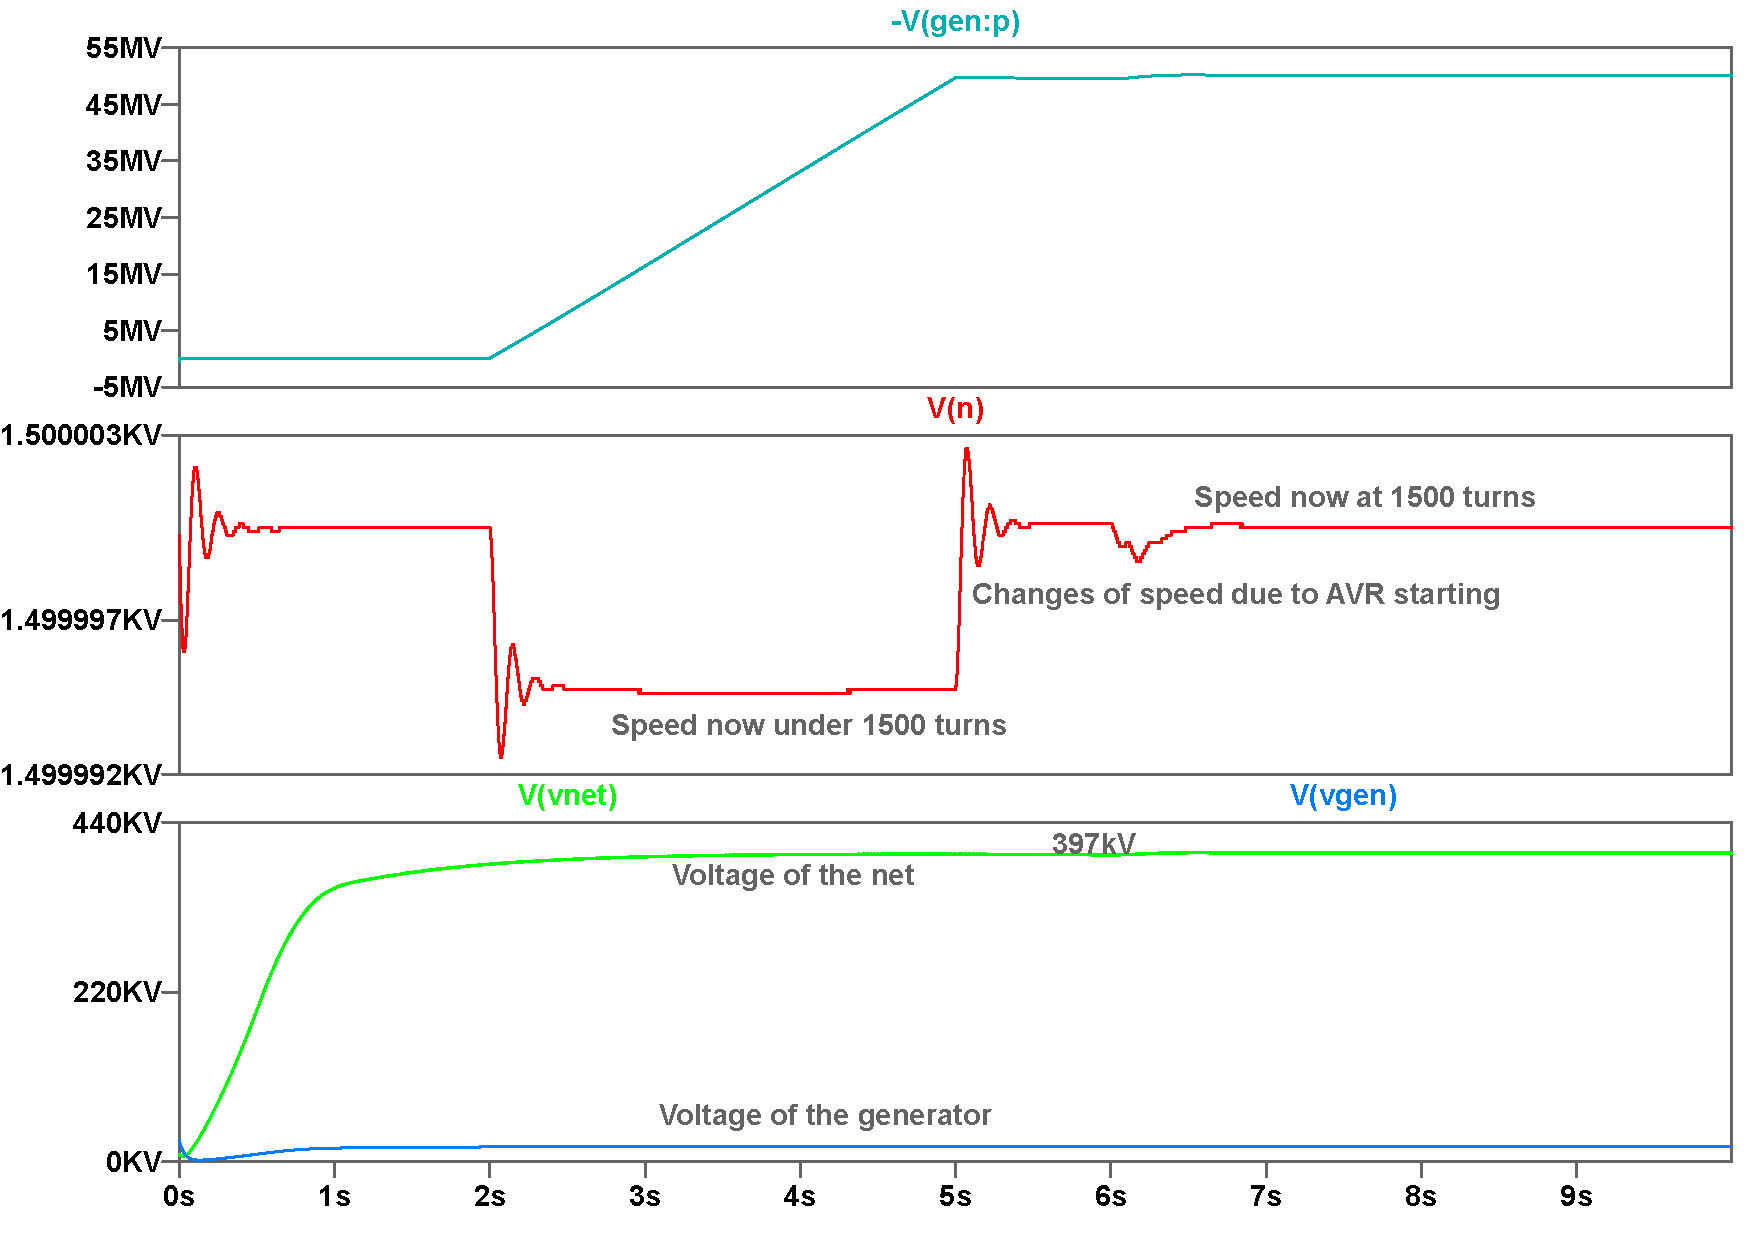
\includegraphics[width=0.9\textwidth] {figures/08_Synchronous_Generator/Synchronous_Generator_Isolated_mode_500MVA/Simulation_Start_Waveform.pdf}
	\caption{Simulaton start - Voltage behaviour - Speed behaviour - Waveform}
	\label{fig:figure82}
\end{figure}

\begin{figure}[H]
	\centering
	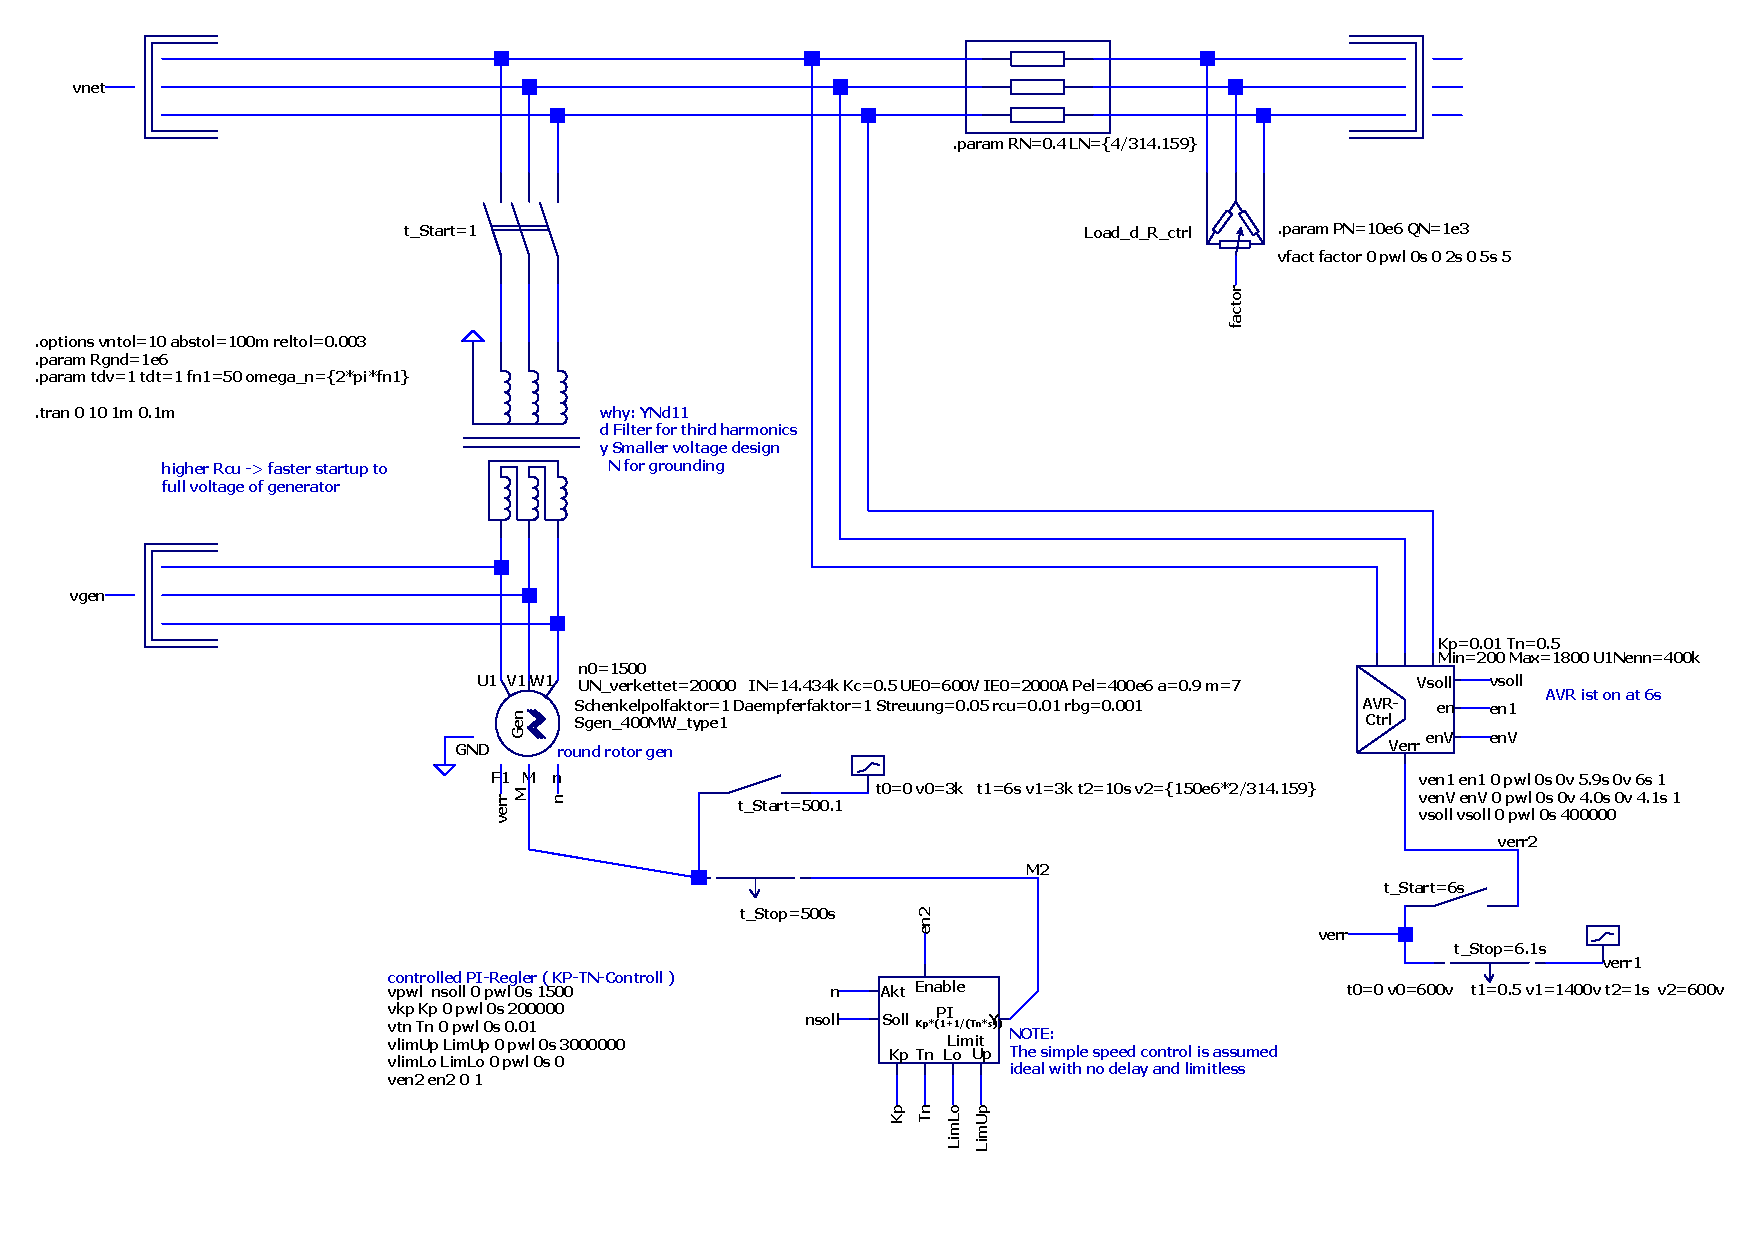
\includegraphics[width=1\textwidth] {figures/08_Synchronous_Generator/Synchronous_Generator_Isolated_mode_500MVA/Load_angle_Schematic.pdf}
	\caption{Load angle - schematic}
	\label{fig:figure83}
\end{figure}

\begin{figure}[H]
	\centering
	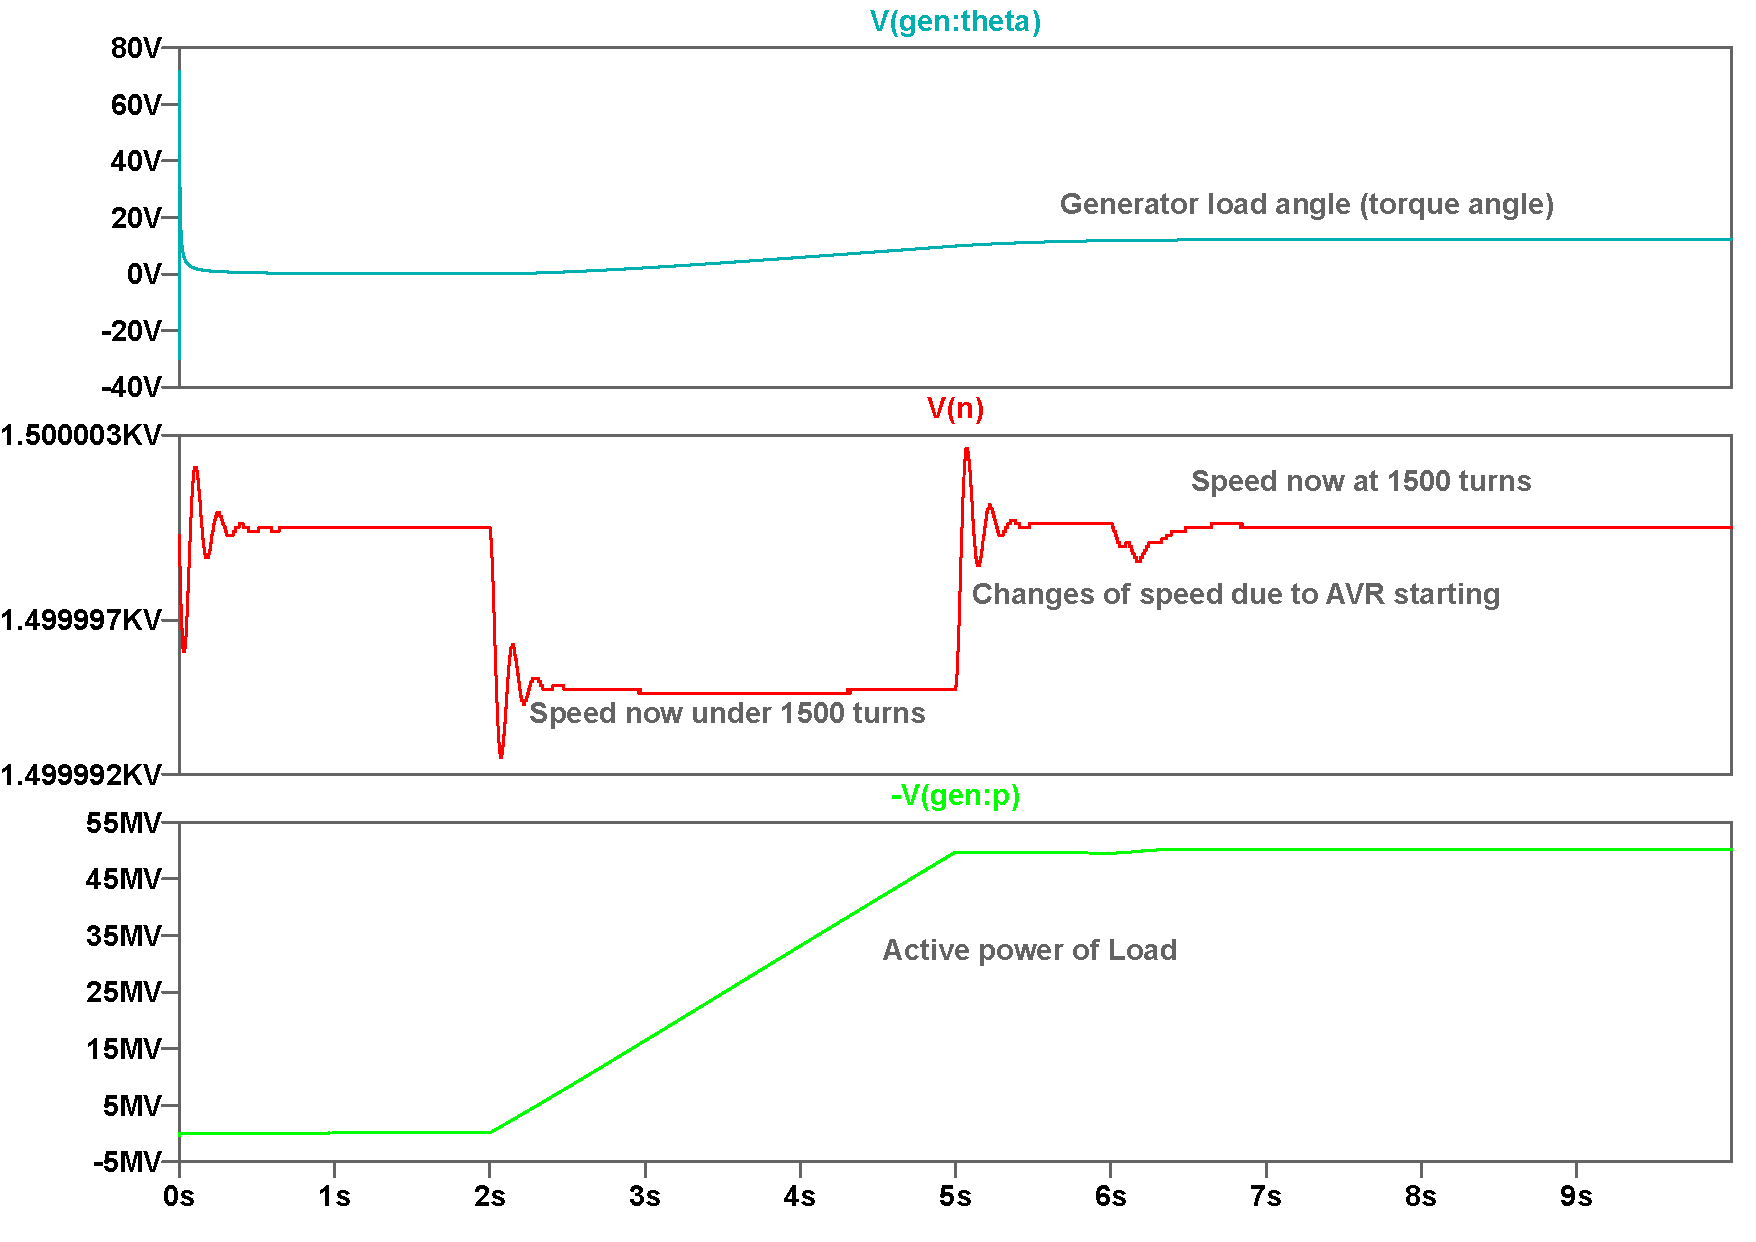
\includegraphics[width=0.9\textwidth] {figures/08_Synchronous_Generator/Synchronous_Generator_Isolated_mode_500MVA/Load_angle_Waveform.pdf}
	\caption{Load angle - Waveform}
	\label{fig:figure84}
\end{figure}

\begin{figure}[H]
	\centering
	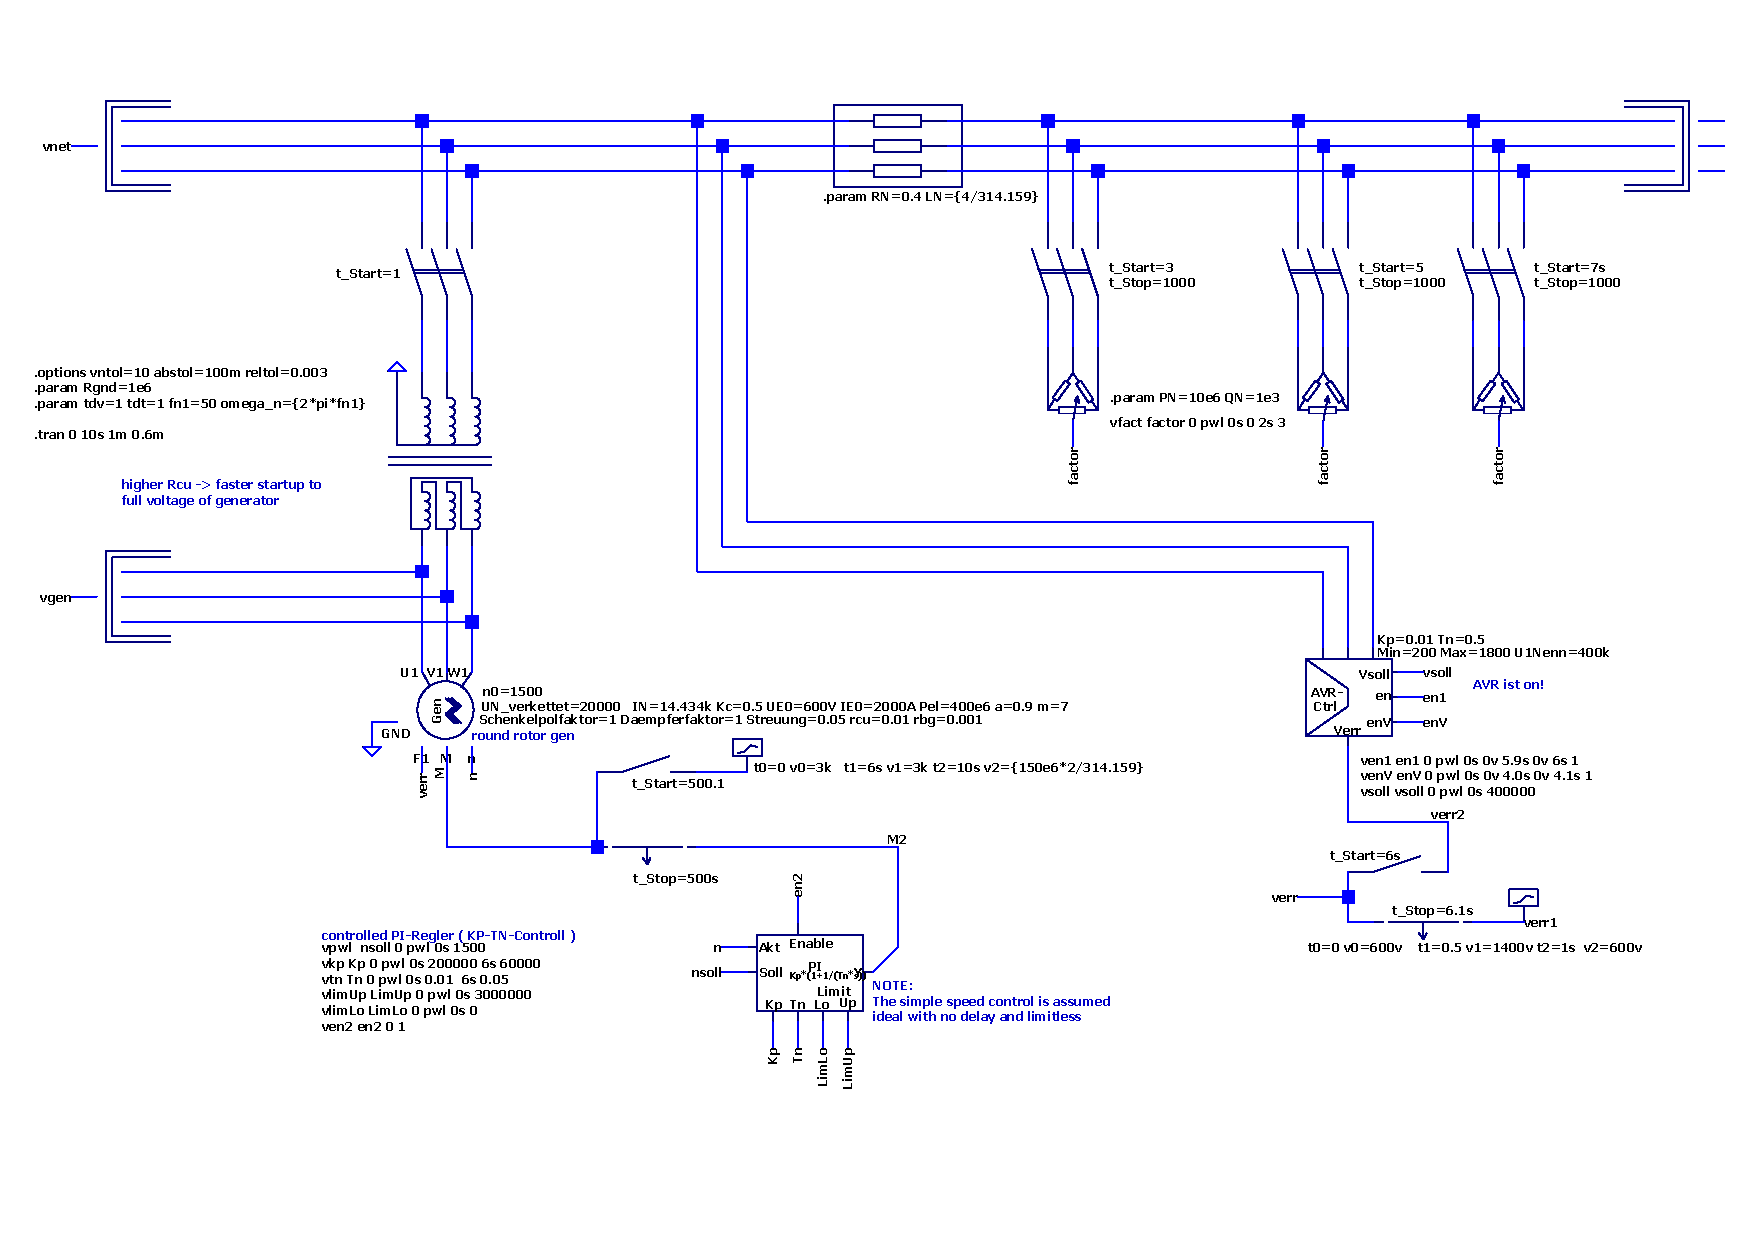
\includegraphics[width=1\textwidth] {figures/08_Synchronous_Generator/Synchronous_Generator_Isolated_mode_500MVA/Load_steps_Schematic.pdf}
	\caption{Load steps - schematic}
	\label{fig:figure85}
\end{figure}

\begin{figure}[H]
	\centering
	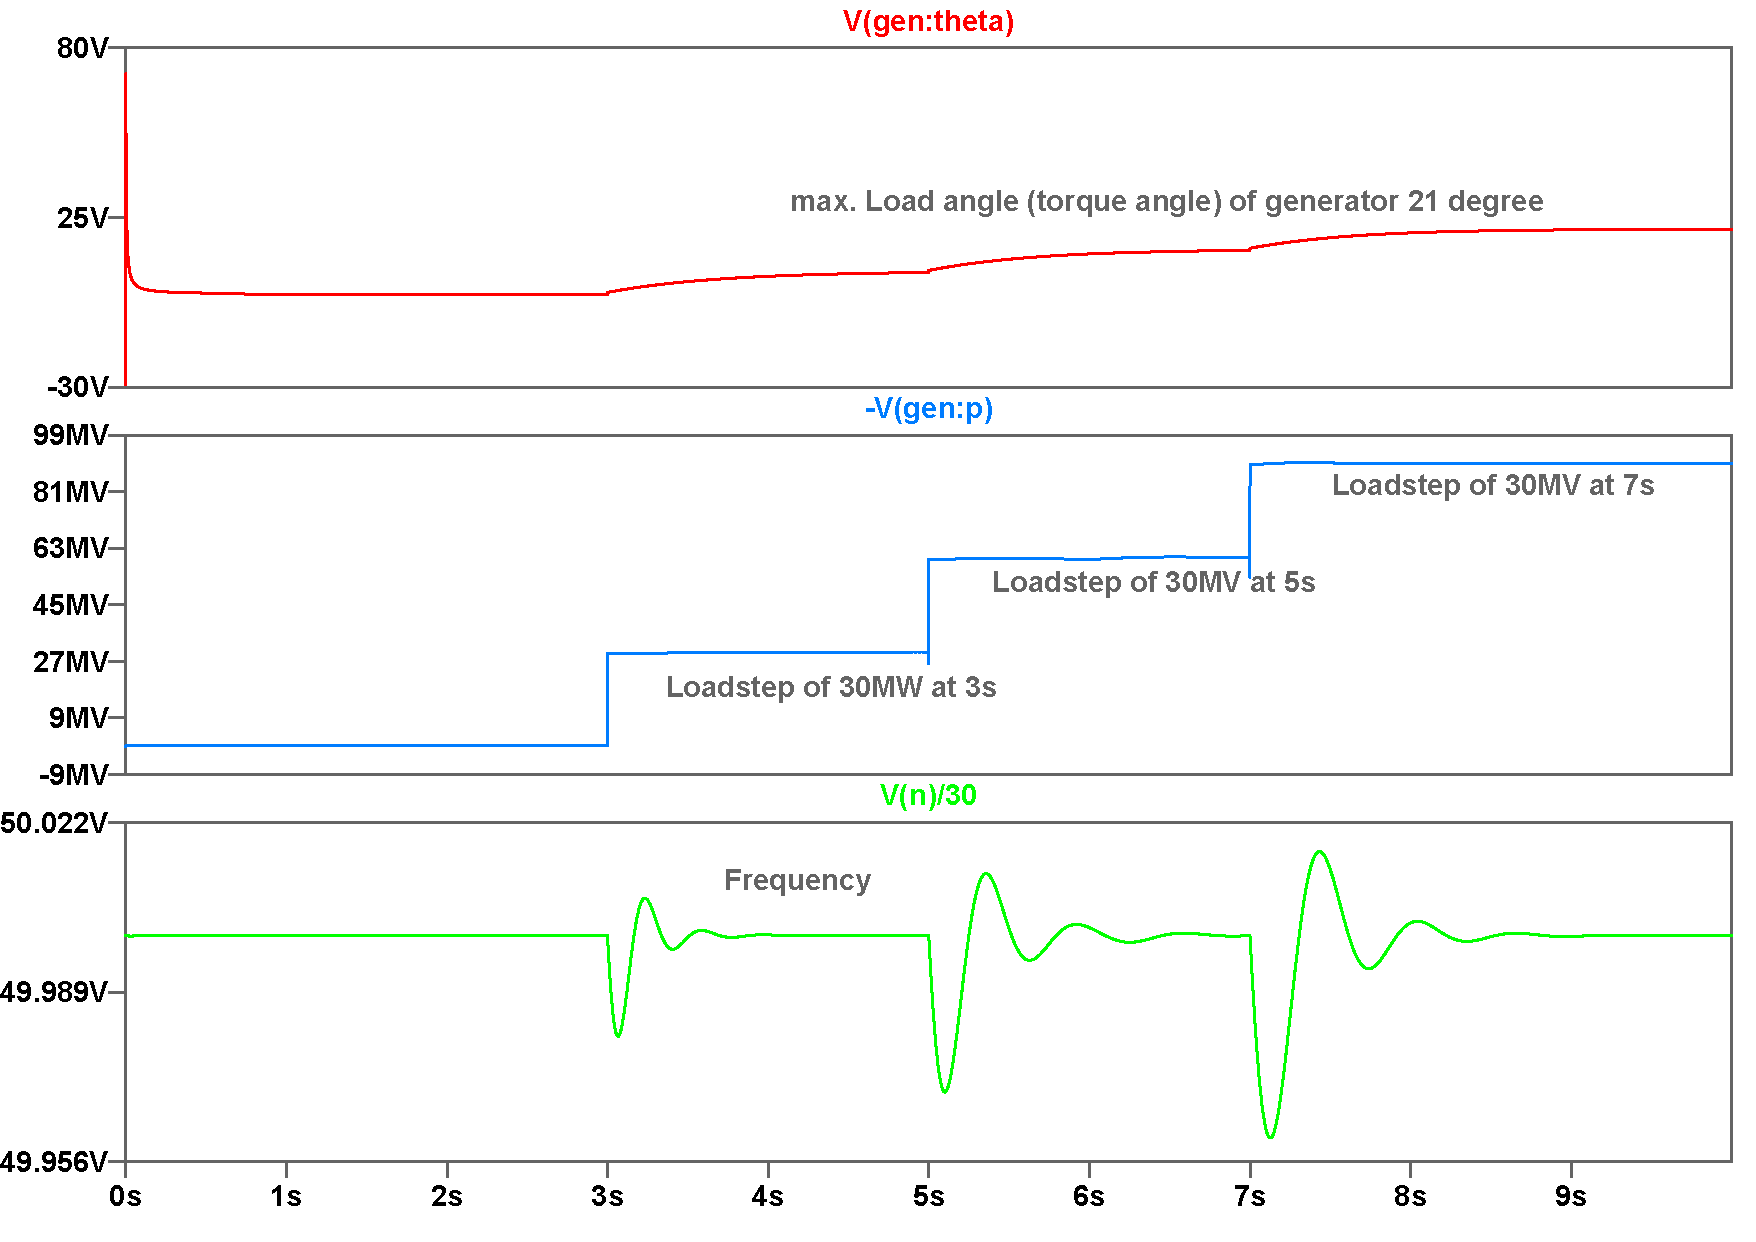
\includegraphics[width=0.9\textwidth] {figures/08_Synchronous_Generator/Synchronous_Generator_Isolated_mode_500MVA/Load_steps_Waveform.pdf}
	\caption{Load steps - Waveform}
	\label{fig:figure86}
\end{figure}


\subsection{Comparison with a Salient-Pole Machine} see figures: \ref{fig:figure87} and \ref{fig:figure88}  (simulation-file: same name as the heading)

The parameter settings \texttt{SchenkelPoleFactor=0.5} and \texttt{KC=0.8}
represent a salient-pole machine in this model. After restarting the
simulation, the load angle is approximately \ang{7}, compared with about
\ang{21} for the round-rotor case. The difference results from the changed
direct- and quadrature-axis reactances and the additional reluctance-torque
component.



\subsection{Reactive Power in Island Operation} 

In an isolated network, the total active and reactive powers are determined by
the connected loads and network losses. Excitation primarily controls the
terminal voltage and the sharing of reactive power between parallel sources.
With only one generator, changing the field voltage cannot independently
specify the reactive power demanded by a constant-power load.

\begin{remark}{Voltage dependence of the load}{rem:island-load-model}
The influence of the AVR on load power depends on the load model. Constant-impedance loads change their power approximately with the square of the
voltage, whereas ideal constant-power loads maintain their specified $P$ and
$Q$ by changing their current.
\end{remark}

\subsection{Switching Off the Loads} see figures: \ref{fig:figure89} and \ref{fig:figure810}  (simulation-file: same name as the heading)

The three loads are disconnected at \SI{9}{\second}, \SI{11}{\second}, and
\SI{13}{\second}. The load angle decreases after each switching operation.
When the final load is removed, the frequency overshoots above its nominal
value, which is the opposite of its response to a positive load step. In the
chosen model, the frequency takes approximately \SI{3.5}{\second} to return
to \SI{50}{\hertz}, because only the governor action and the comparatively
small friction torque decelerate the rotor.

\subsection{Scaling Quantities in the Waveform Viewer} 

Internal signals are always in Volt and can be displayed in engineering units by using the following scale factors in LTspice: e.g 
multiplying a trace for active power (in volt) by 1W/1V gives the
correct unit now in W.

\begin{center}
\renewcommand{\arraystretch}{1.15}
\begin{tabularx}{0.86\textwidth}{@{}l l X@{}}
\toprule
\textbf{Quantity} & \textbf{Scale factor} & \textbf{Displayed unit} \\
\midrule
Load angle & $1\,\mathrm{deg}/\mathrm{V}$ & degree \\
Frequency  & $1\,\mathrm{Hz}/\mathrm{V}$  & hertz \\
Active power & $1\,\mathrm{W}/\mathrm{V}$ & watt \\
\bottomrule
\end{tabularx}
\end{center}

\newpage


\begin{figure}[H]
	\centering
	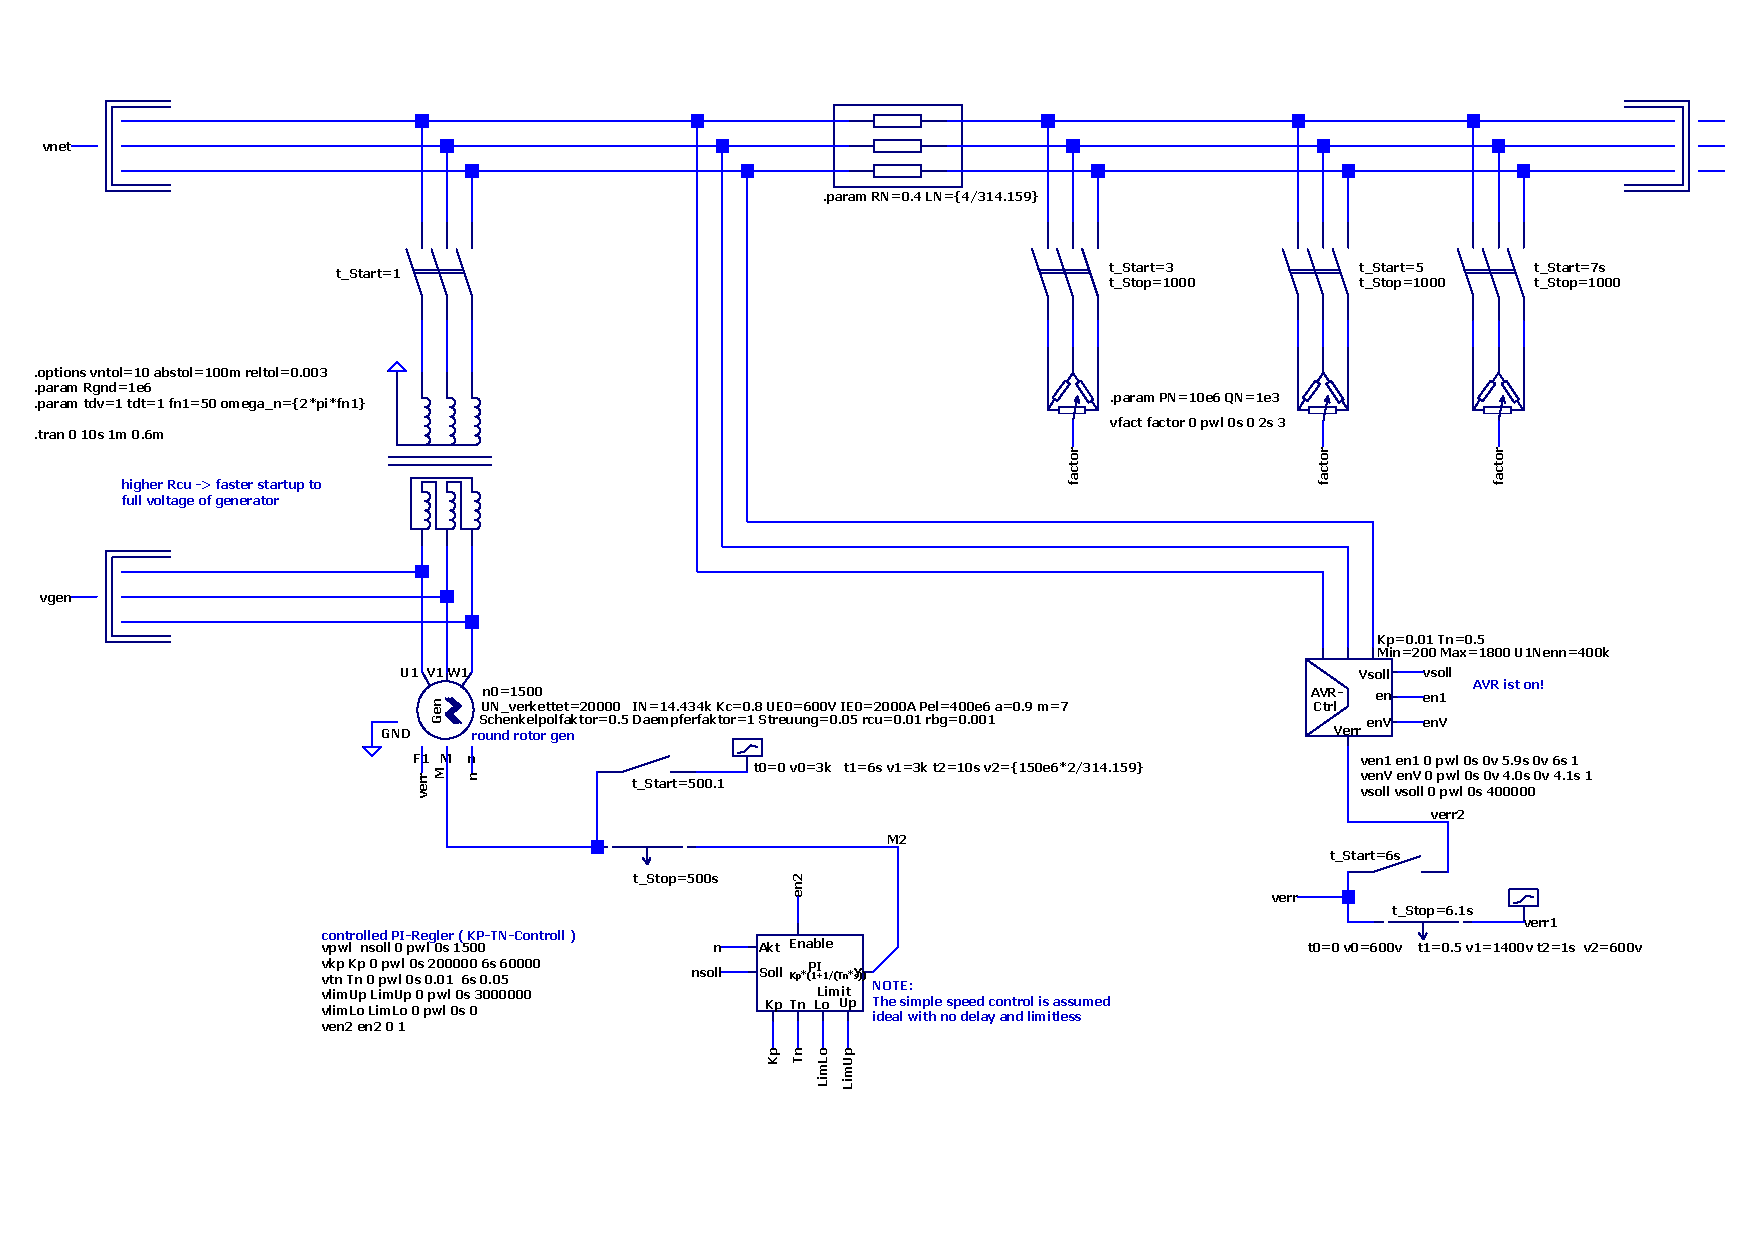
\includegraphics[width=1\textwidth] {figures/08_Synchronous_Generator/Synchronous_Generator_Isolated_mode_500MVA/Salientpole_IslandOperation_Schematic.pdf}
	\caption{Comparison with a salient-pole machine - schematic}
	\label{fig:figure87}
\end{figure}

\begin{figure}[H]
	\centering
	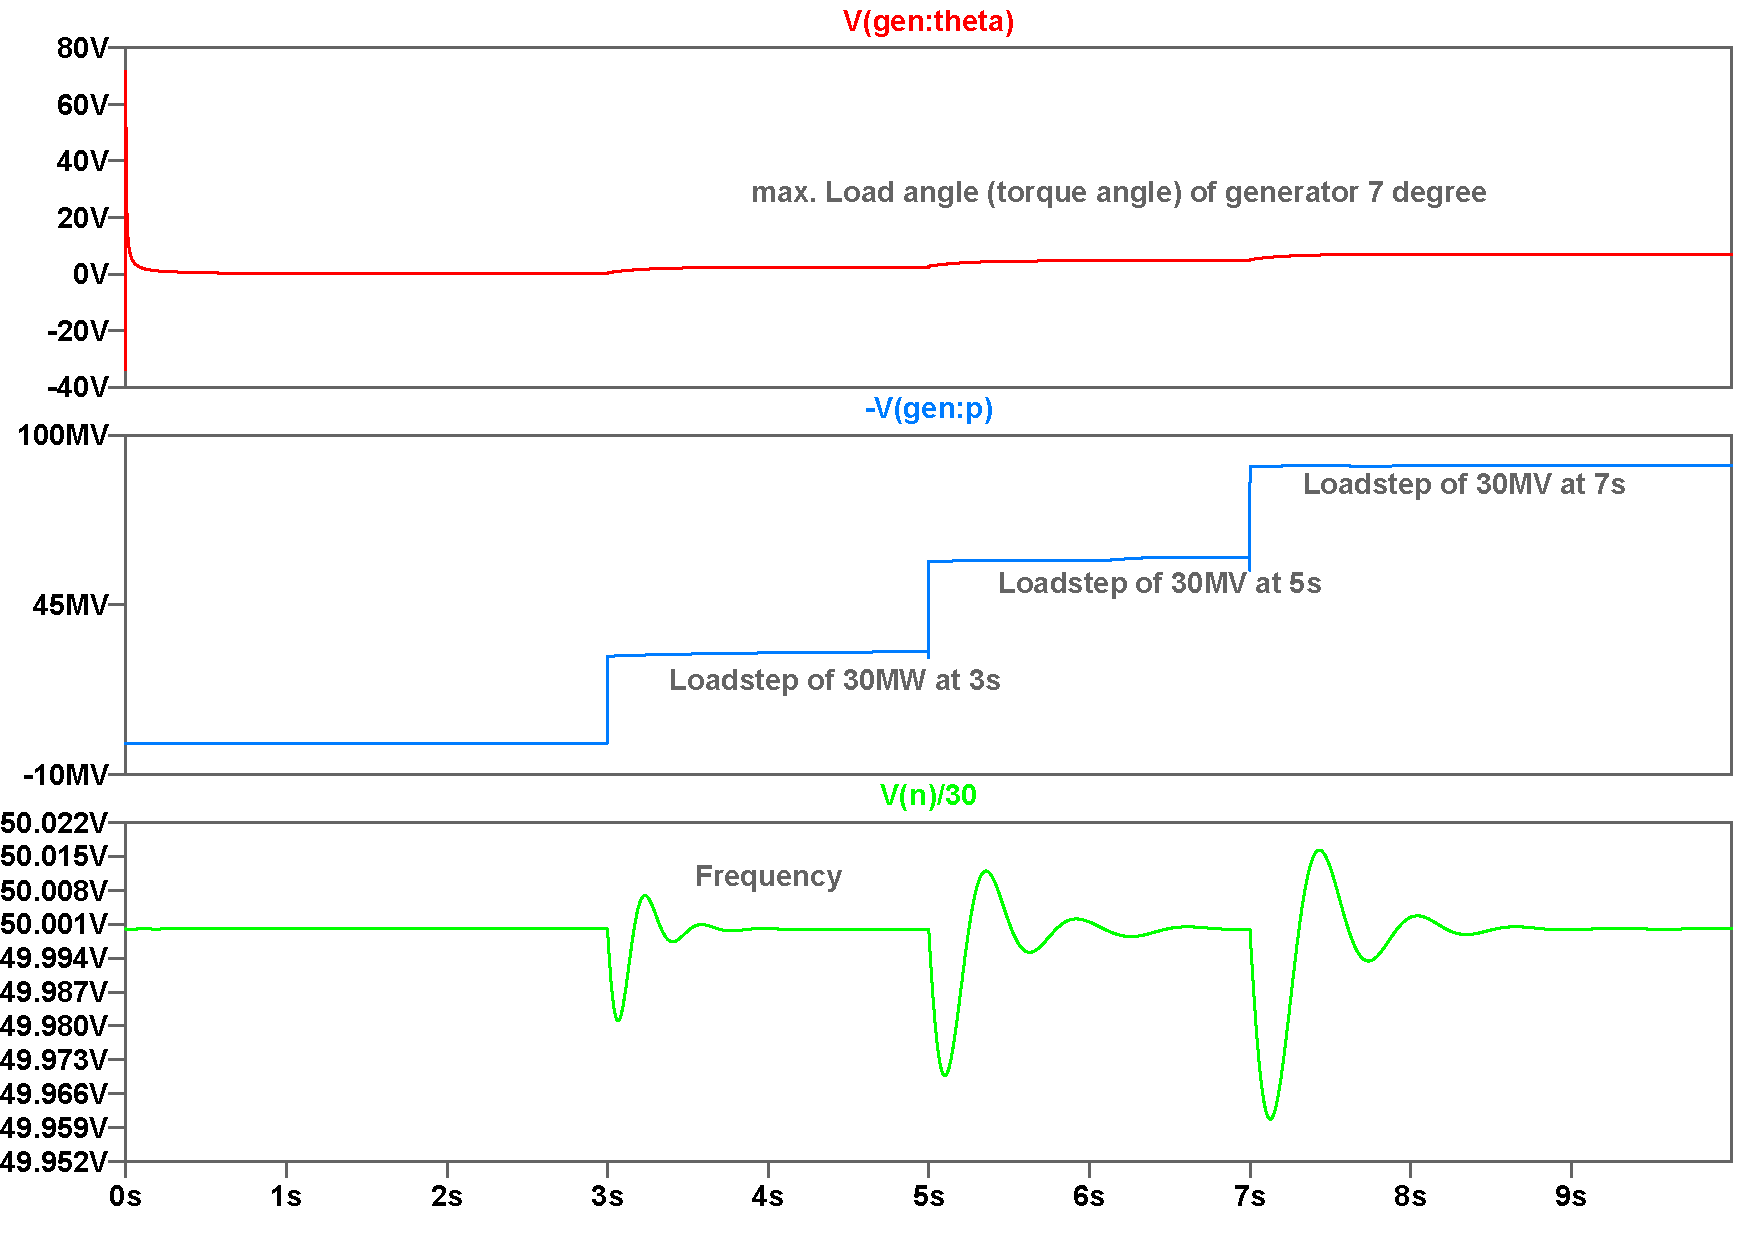
\includegraphics[width=0.9\textwidth] {figures/08_Synchronous_Generator/Synchronous_Generator_Isolated_mode_500MVA/Salientpole_IslandOperation_Waveform.pdf}
	\caption{Comparison with a salient-pole machine - Waveform}
	\label{fig:figure88}
\end{figure}

\begin{figure}[H]
	\centering
	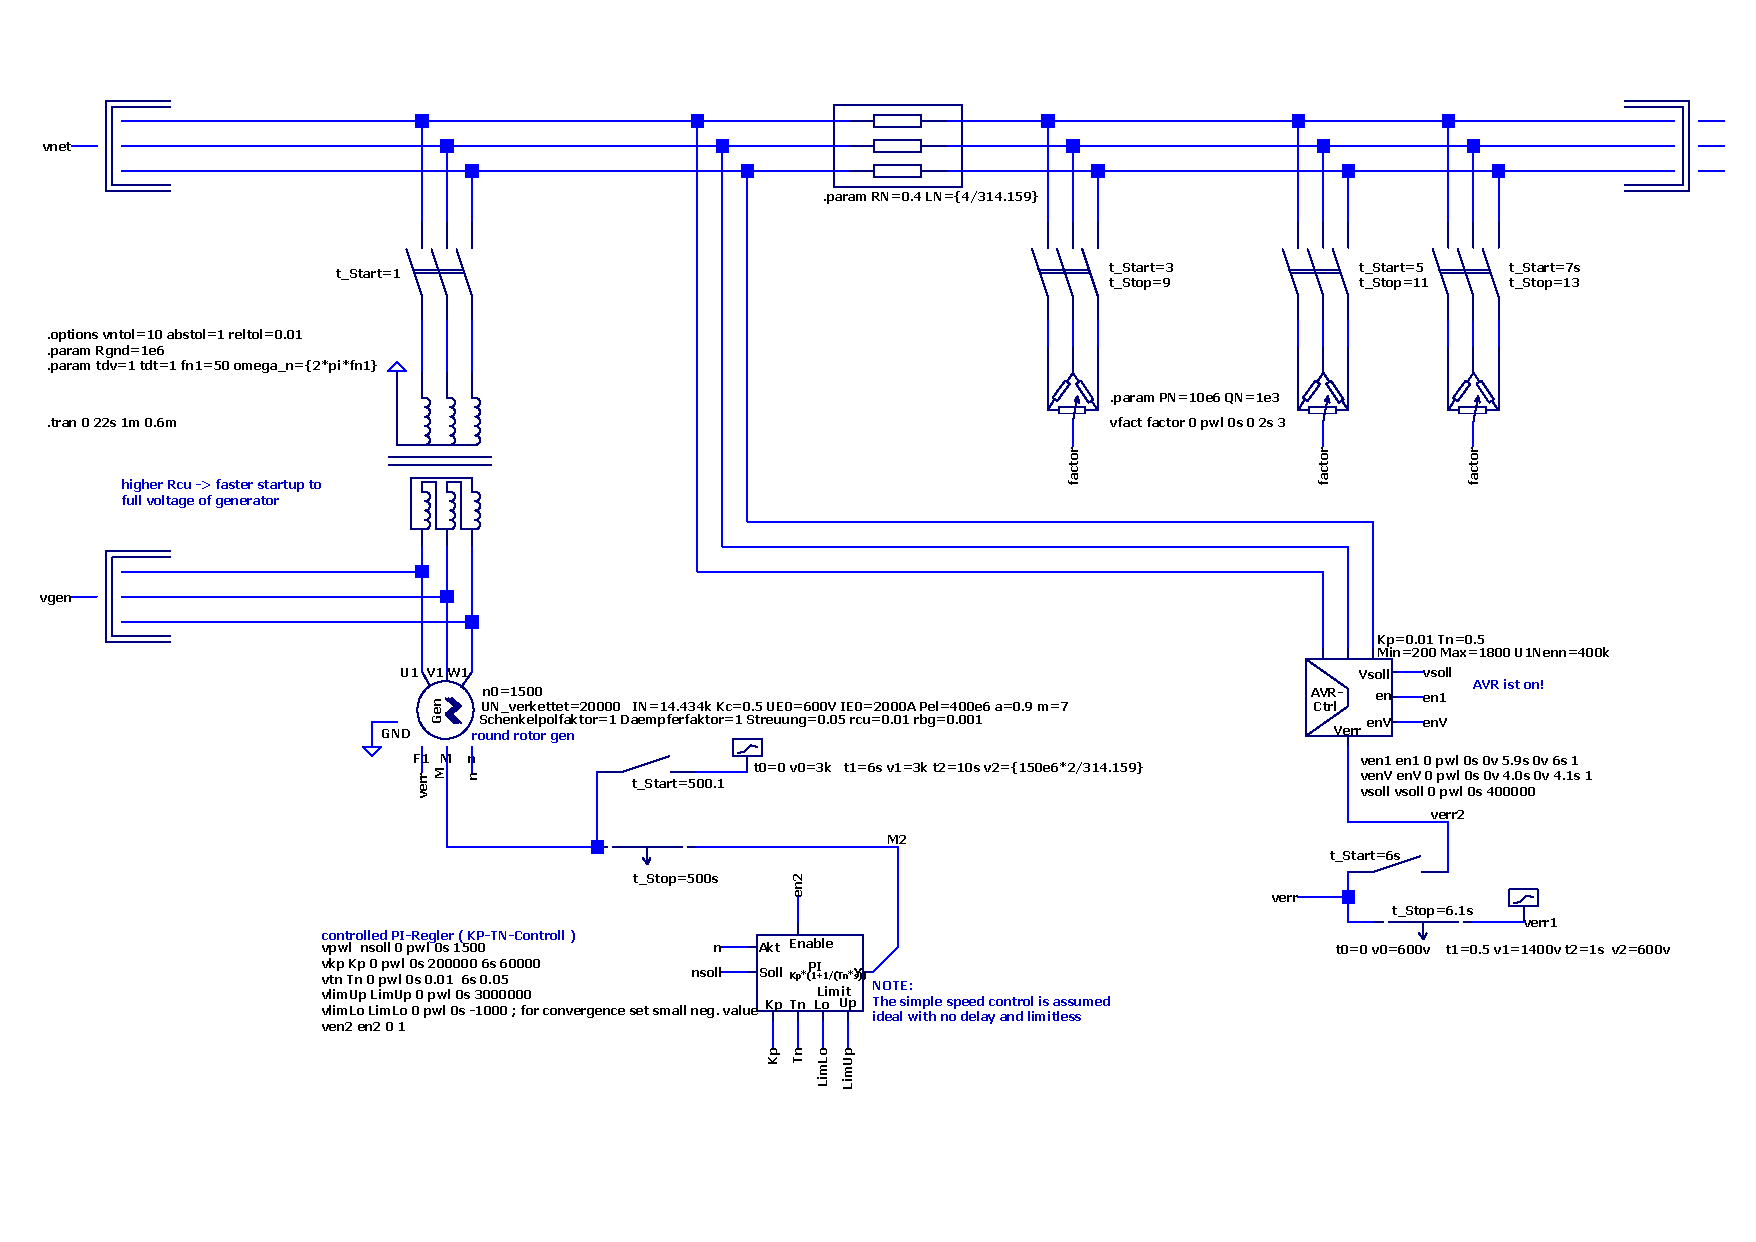
\includegraphics[width=1\textwidth] {figures/08_Synchronous_Generator/Synchronous_Generator_Isolated_mode_500MVA/Switching_off_loads_Schematic.pdf}
	\caption{Switching off loads - schematic}
	\label{fig:figure89}
\end{figure}

\begin{figure}[H]
	\centering
	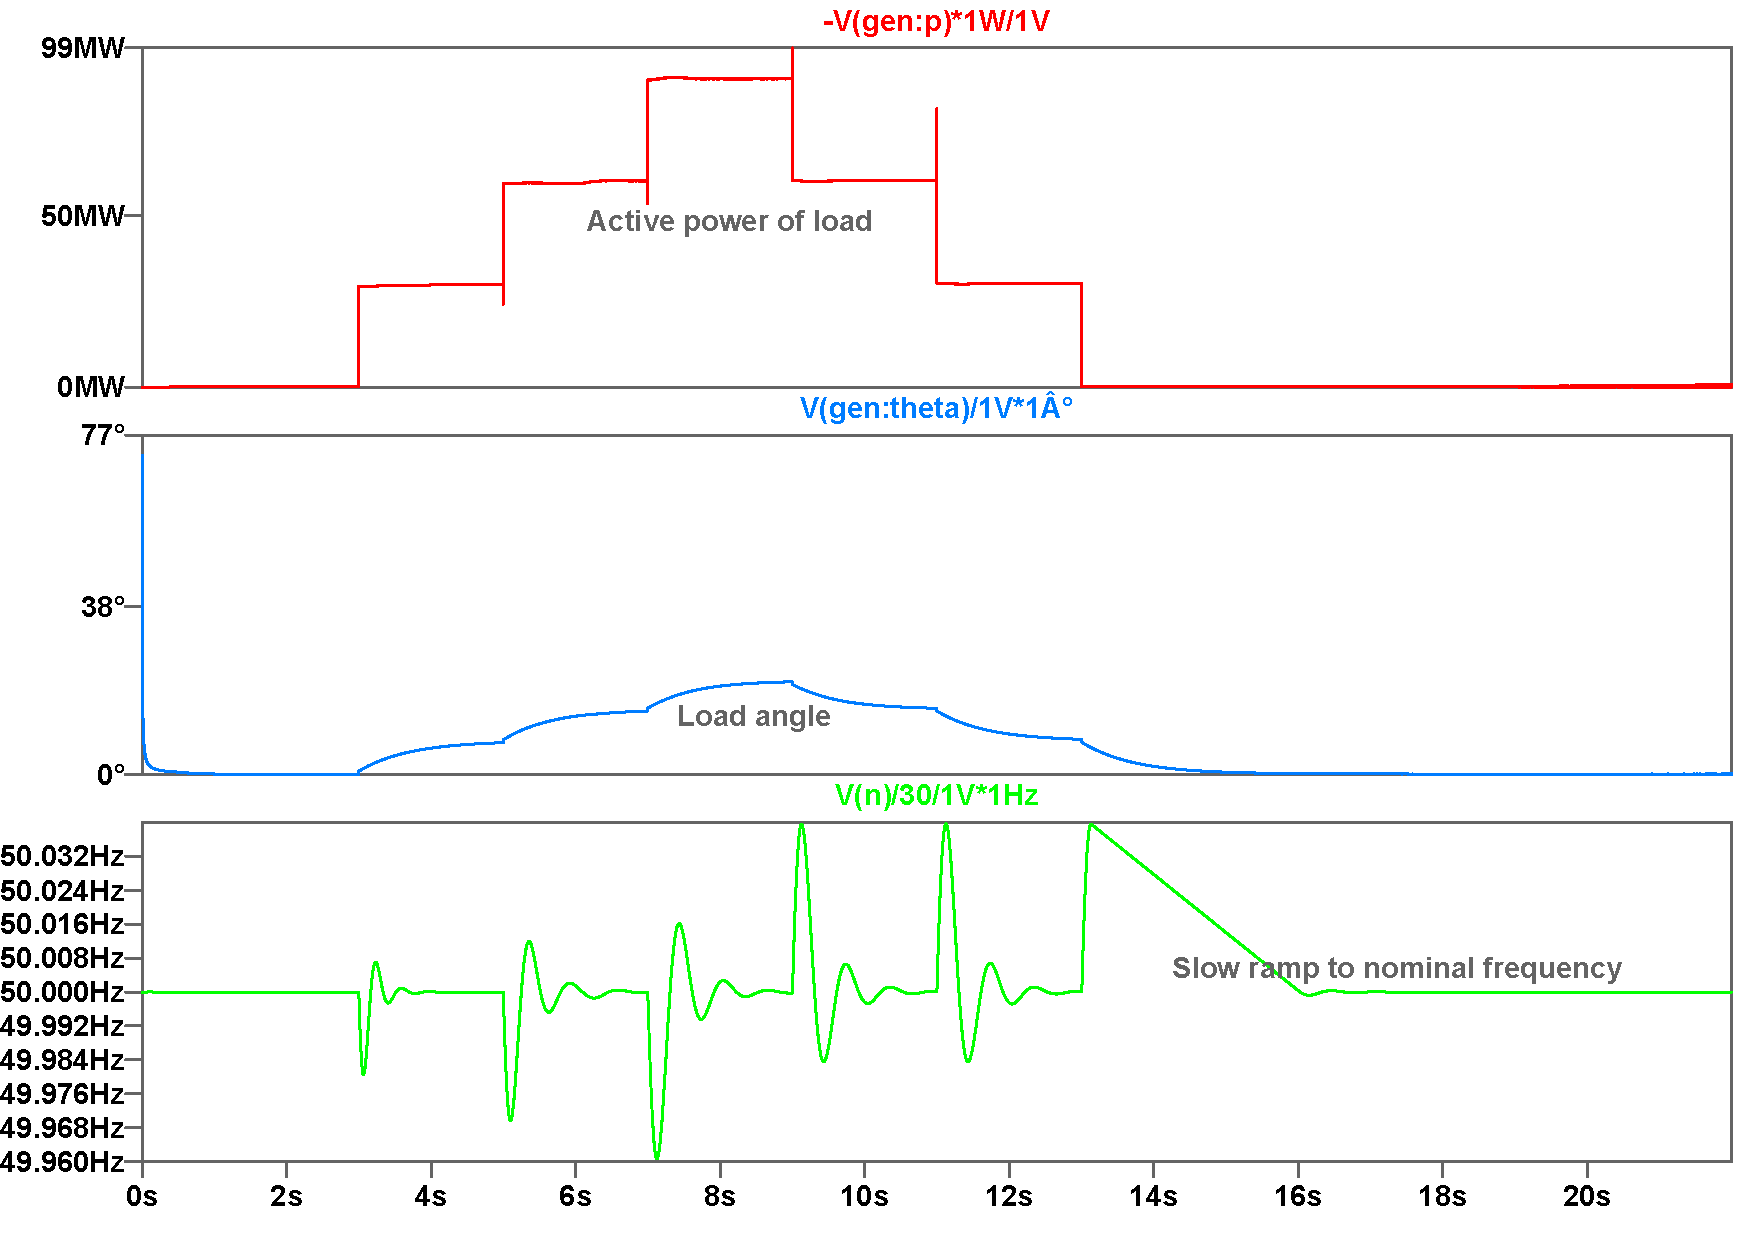
\includegraphics[width=0.9\textwidth] {figures/08_Synchronous_Generator/Synchronous_Generator_Isolated_mode_500MVA/Switching_off_loads_Waveform.pdf}
	\caption{Switching off loads - Waveform}
	\label{fig:figure810}
\end{figure}

\subsection{Synchronizing a Second Generator} see figures \ref{fig:figure811}-\ref{fig:figure813}  (simulation-file: same name as the heading)

A second generator is added on the right-hand side together with its speed
controller, but without an active AVR in this particular demonstration. The
simulation end time is increased to \SI{30}{\second}. Generator~2 is connected
at \SI{12}{\second}; its speed controller is disabled at that instant, and a
constant-torque input becomes active at \SI{12.1}{\second}. A ramp from zero
to \SI{20}{\mega\watt} between \SI{14}{\second} and
\SI{18}{\second} establishes its active-power output. A third load is switched
at \SI{20}{\second} to examine the response after synchronization.

\subsubsection{Synchronization Conditions} see figures \ref{fig:figure811} and \ref{fig:figure812} and \ref{fig:figure813}

Between approximately \SI{9.8}{\second} and \SI{10.2}{\second}, the generator
and network voltages have nearly equal magnitudes, although Generator~2 leads
slightly in phase. Its speed reference can be reduced from \SI{50}{\hertz} to
\SI{49.98}{\hertz}, corresponding to a small negative slip. At
\SI{12}{\second}, the two voltages are approximately in phase and the switch
can be closed.

\begin{important}{Conditions before synchronization}{imp:synchronization}
Before connecting a synchronous generator to an energized network, verify the
phase sequence, voltage magnitude, frequency, and phase angle. Closing the
switch with an excessive mismatch can produce high currents and severe shaft-torque transients.
\end{important}

\subsubsection{Power Sharing} see figures \ref{fig:figure811} and \ref{fig:figure812} and \ref{fig:figure813}

Generator~2 supplies \SI{20}{\mega\watt}, so Generator~1 reduces its output to
approximately \SI{40}{\mega\watt}. A subsequent
\SI{30}{\mega\watt} load step is supplied almost entirely by Generator~1,
because the active-power controller of Generator~2 has been disabled. The final
outputs are therefore approximately \SI{70}{\mega\watt} for Generator~1 and
\SI{20}{\mega\watt} for Generator~2. Generator~2 exhibits larger transient
speed deviations because it has no active governor in this example.

\begin{remark}{Regulation of parallel generators}{rem:parallel-regulation}
Disabling the AVR and governor of Generator~2 is a deliberate simplification
of this example, not a general operating rule. In practical island systems,
parallel generators normally retain coordinated voltage and speed control with
appropriate droop settings.
\end{remark}

\begin{figure}[H]
	\centering
	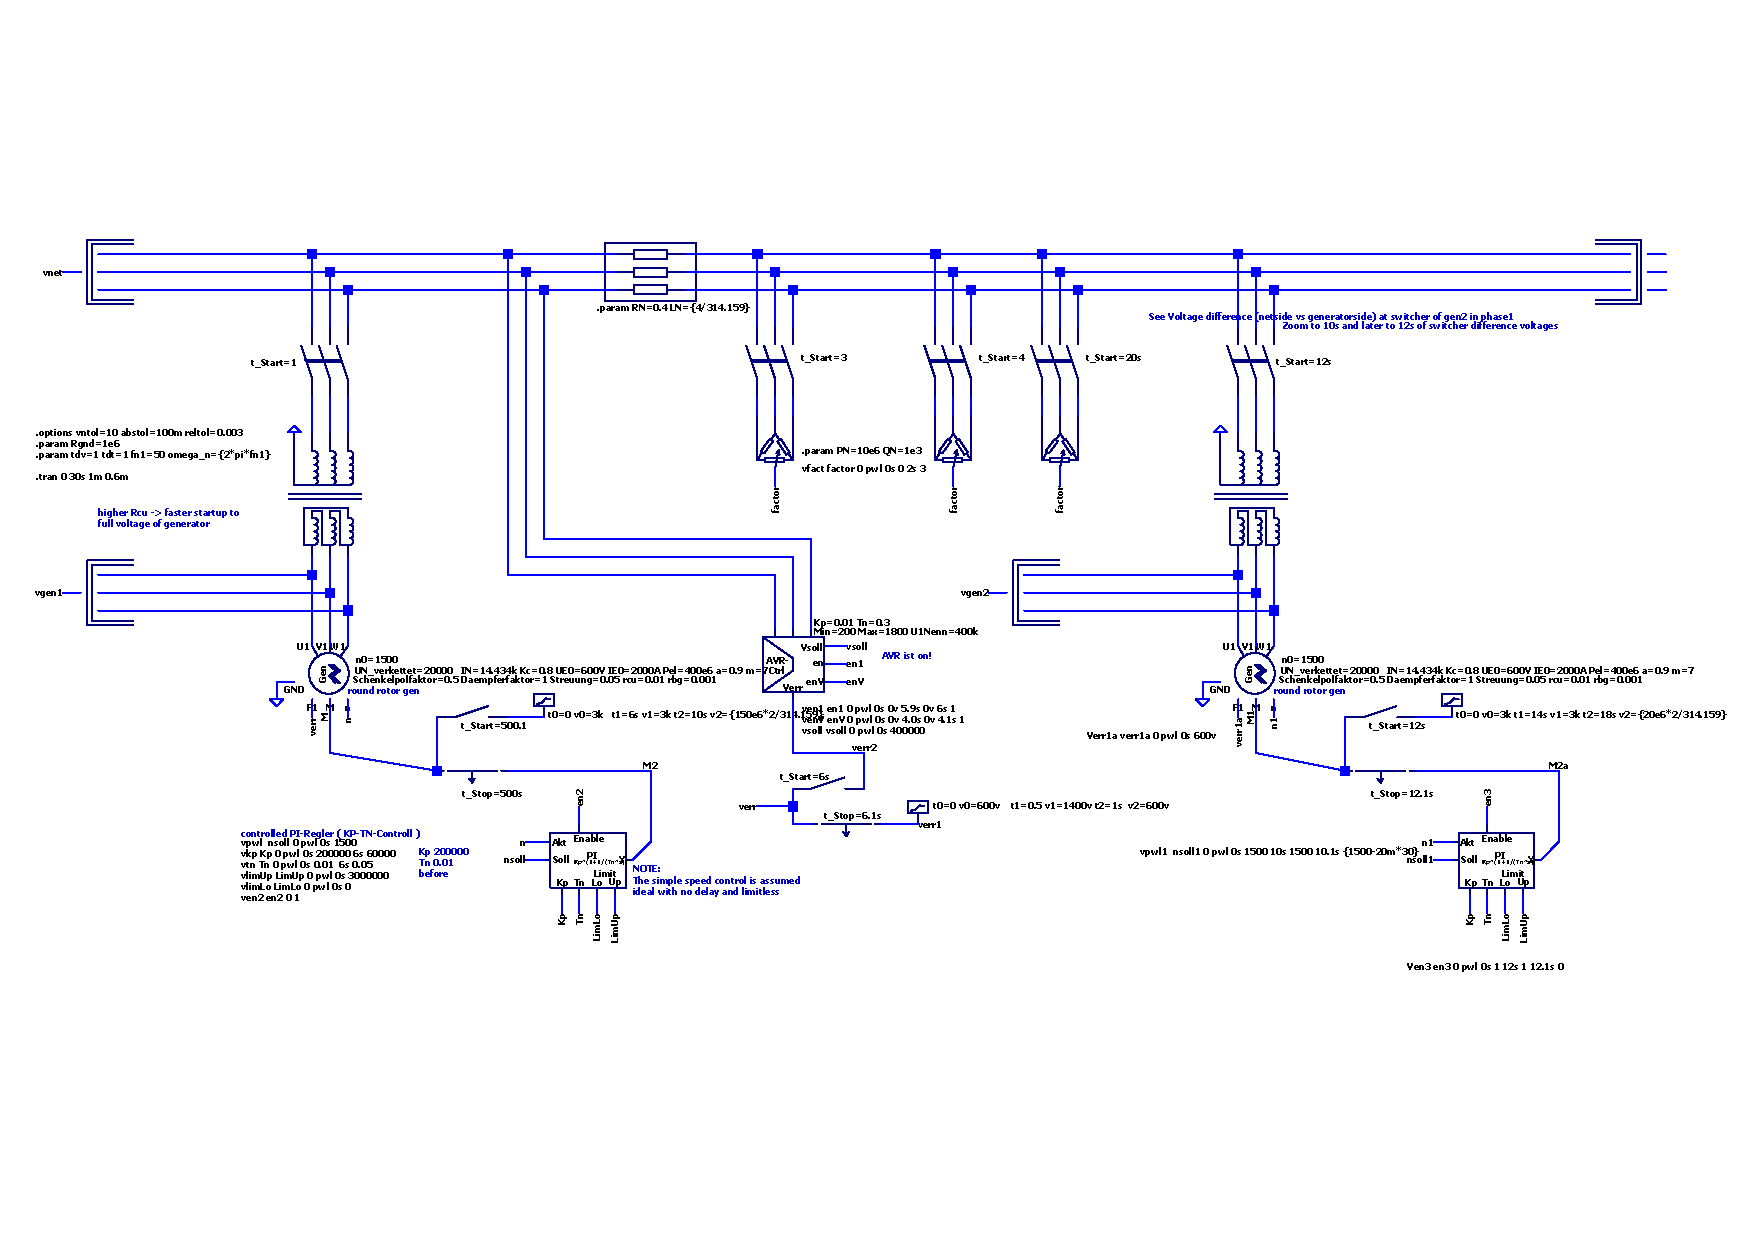
\includegraphics[width=1\textwidth] {figures/08_Synchronous_Generator/Synchronous_Generator_Isolated_mode_500MVA/Synchronizing_a_second_generator_Schematic.pdf}
	\caption{Synchronizing a second generator - schematic}
	\label{fig:figure811}
\end{figure}

\begin{figure}[H]
	\centering
	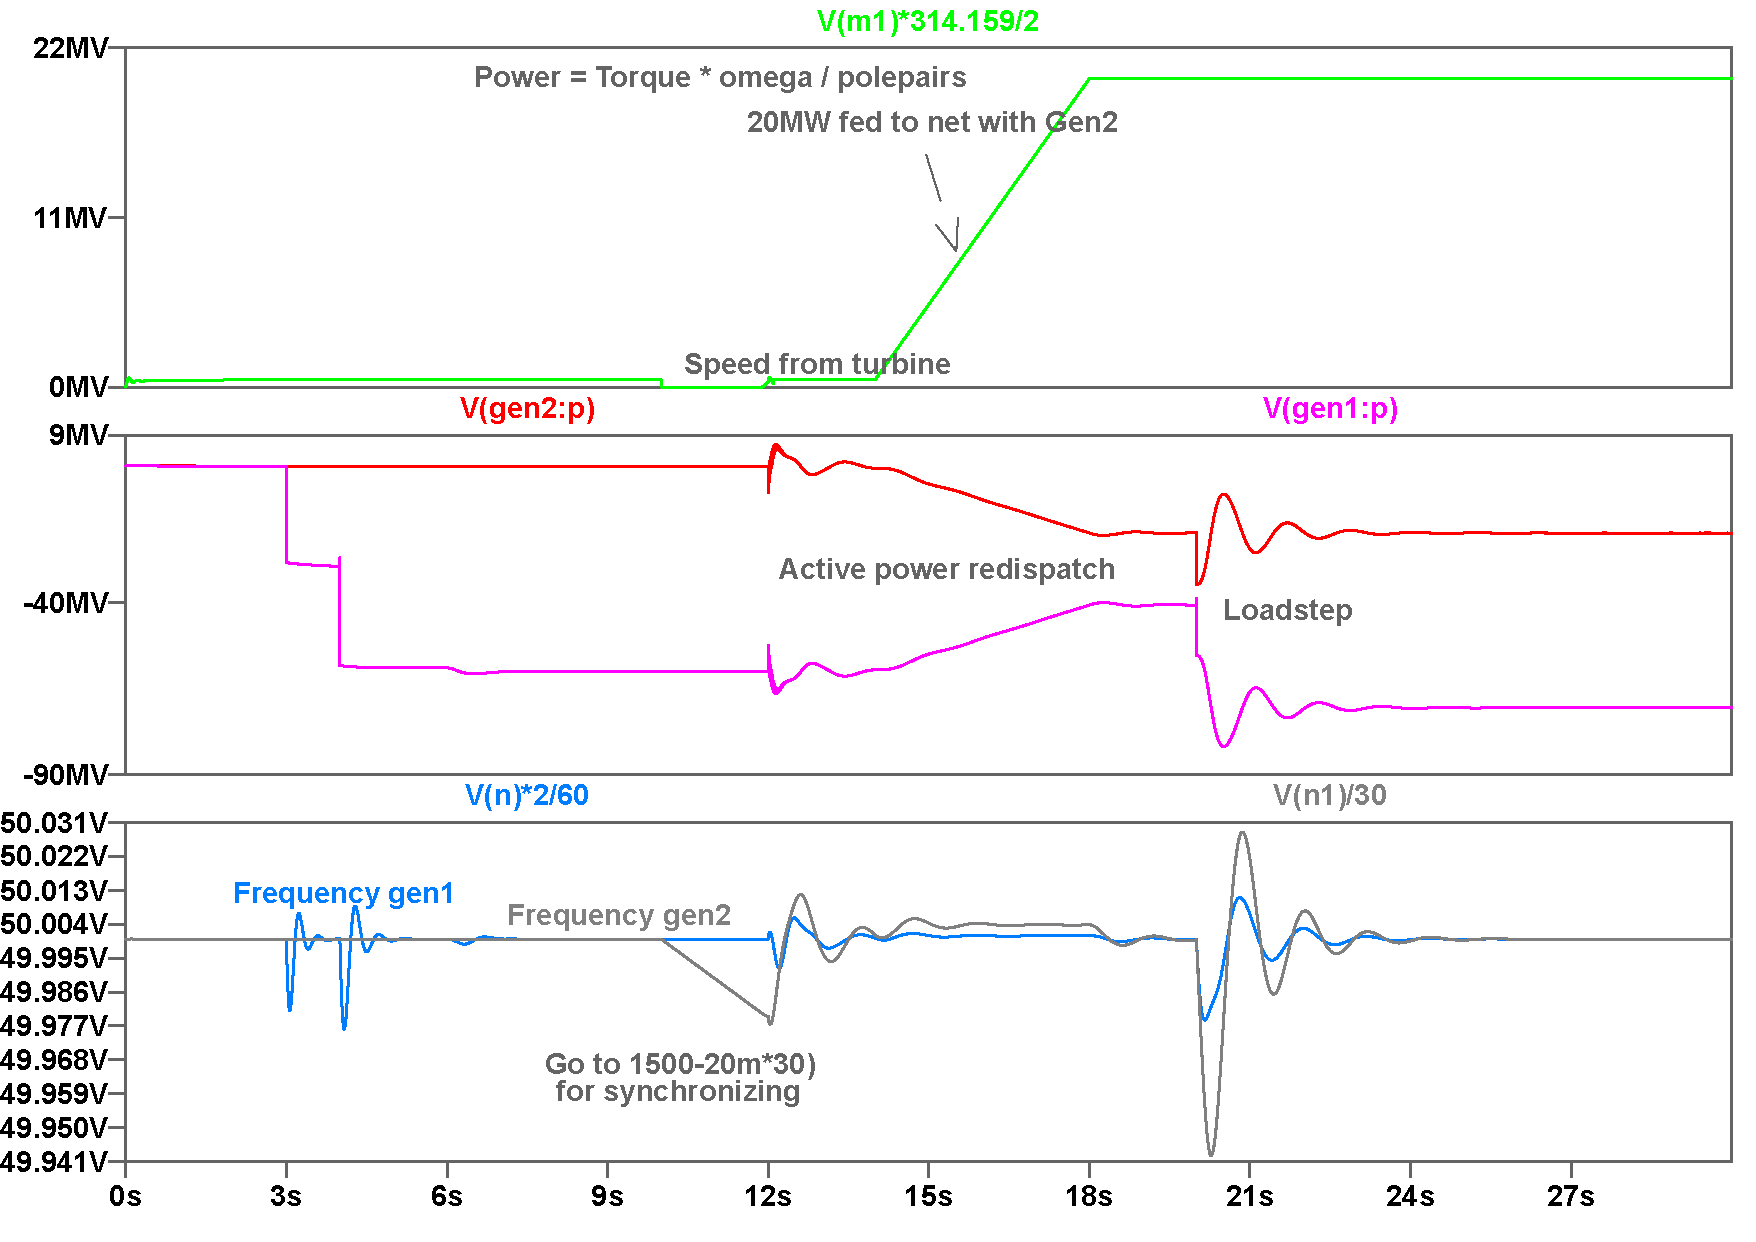
\includegraphics[width=0.9\textwidth] {figures/08_Synchronous_Generator/Synchronous_Generator_Isolated_mode_500MVA/Synchronizing_a_second_generator_Waveform.pdf}
	\caption{Synchronizing a second generator - Waveform}
	\label{fig:figure812}
\end{figure}

\begin{figure}[H]
	\centering
	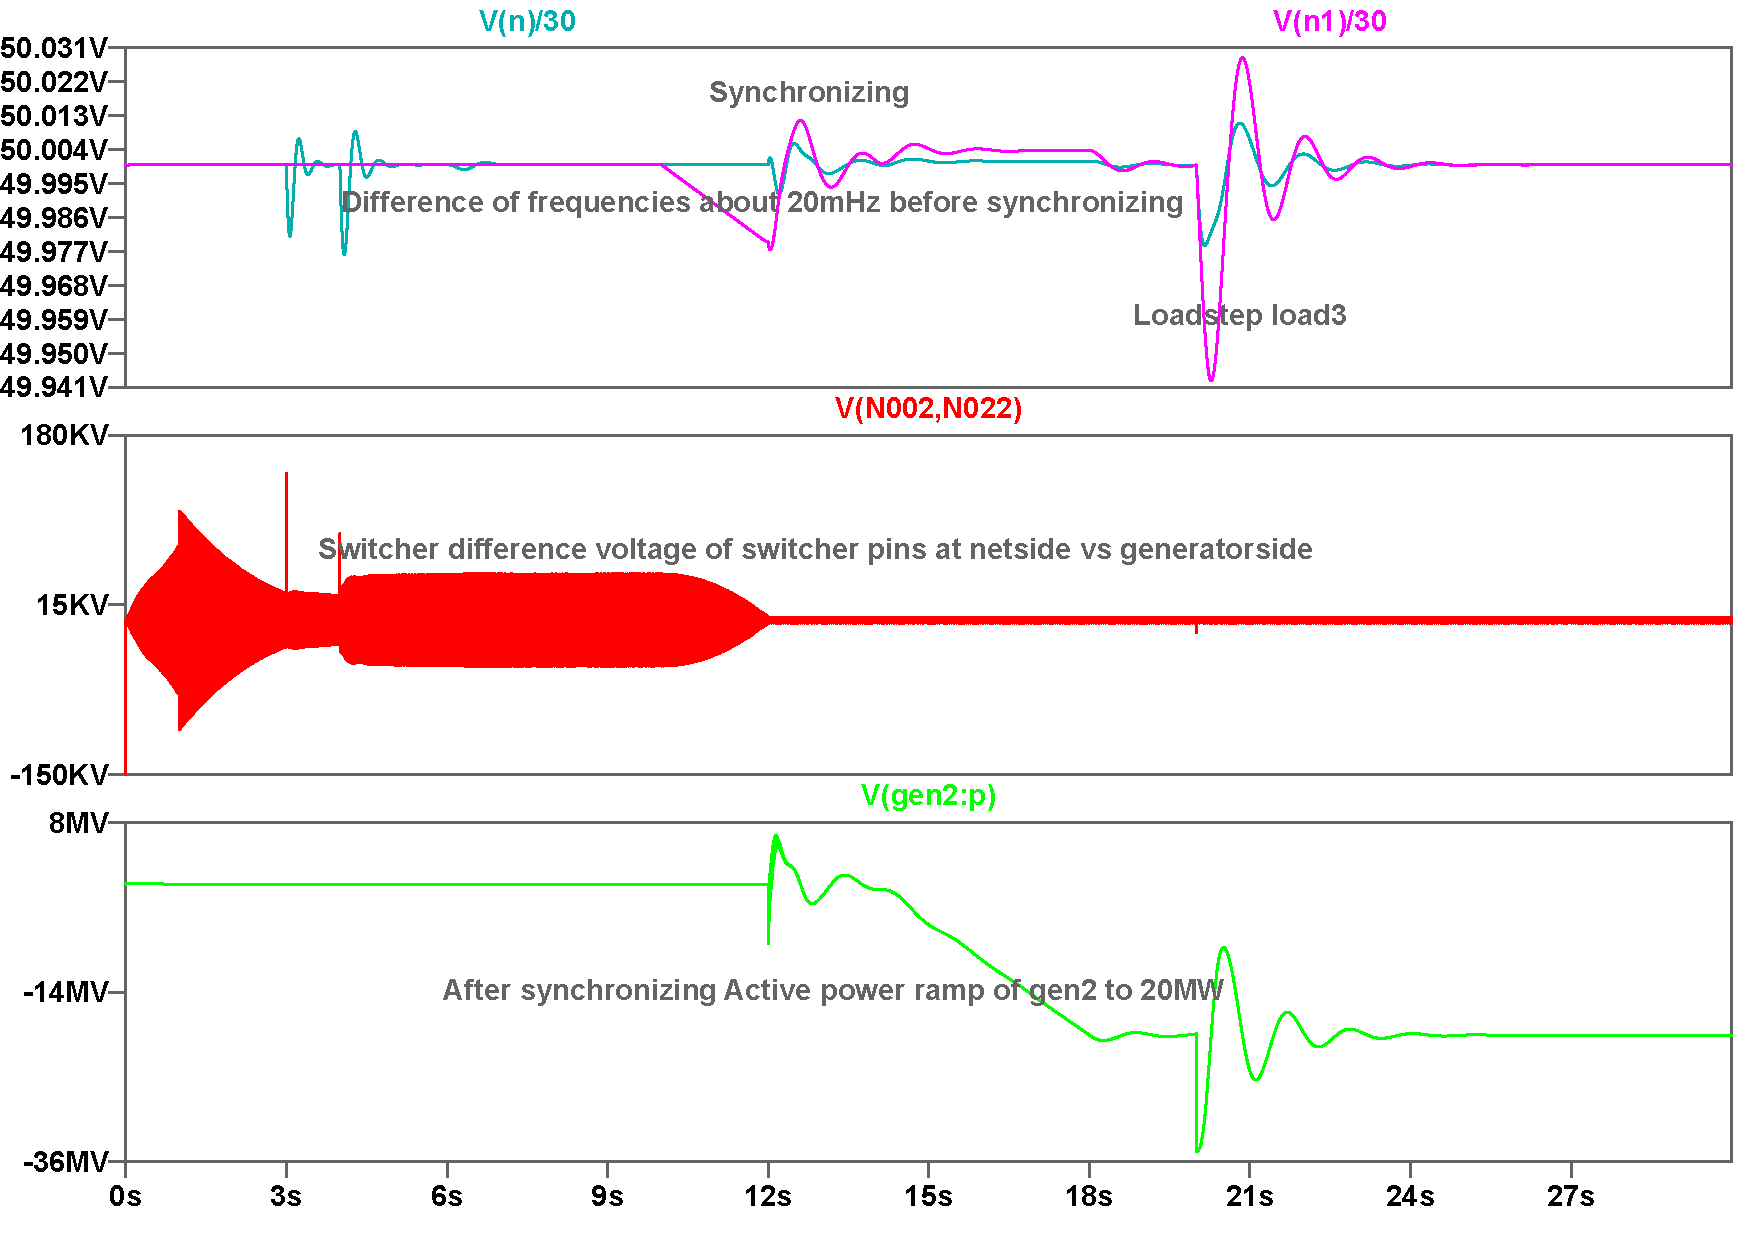
\includegraphics[width=0.9\textwidth] {figures/08_Synchronous_Generator/Synchronous_Generator_Isolated_mode_500MVA/Synchronizing_a_second_generator_Waveform2.pdf}
	\caption{Synchronizing a second generator - Waveform2}
	\label{fig:figure813}
\end{figure}


\newpage

% ============================================================
\section{Grid-Connected and Constant-Speed Operation}
\label{sec:sg-grid-and-fixed-speed}
% ============================================================

\subsection{General}

The following simulations examine synchronization with a stiff grid and the
subsequent delivery of active and reactive power. They also cover faults near
and far from the generator, a single-phase-to-ground fault, operation at fixed
speed, and the loss of synchronism when the transferable active power is
exceeded.

\subsection{Circuit Design}

From left to right, the circuit \texttt{Synchronization\_and\_active\_Power\_output.asc} contains:

\begin{itemize}
  \item a \SI{250}{\mega\volt\ampere}, \SI{13.8}{\kilo\volt},
        \SI{60}{\hertz} synchronous generator rated at
        \SI{3600}{\rpm};
  \item a speed governor and a \SI{5}{\mega\watt} auxiliary load;
  \item an AVR measuring the \SI{13.8}{\kilo\volt} generator bus;
  \item a Yd11 step-up transformer;
  \item a synchronization switch and a \SI{10}{\mega\watt} load;
  \item a switch for a three-phase-to-ground fault; and
  \item a grid impedance and a \SI{230}{\kilo\volt} stiff voltage source.
\end{itemize}

The high-voltage transformer winding is star-connected, while the
generator-side winding is delta-connected. The delta provides a path for
triplen harmonic currents. For the synchronization study, the transformer is
made linear with \texttt{M=1}; the model parameter \texttt{err0=1} is also used
to suppress nonlinear energization transients when full voltage is applied.

The rated excitation voltage is \SI{200}{\volt}. The AVR is enabled at
\SI{0.1}{\second} and provides an excitation range from
\SI{100}{\volt} to \SI{400}{\volt}, allowing both underexcited and
overexcited operation. The speed governor starts with a reference of
\SI{3600}{\rpm}.

The generator is synchronized at \SI{1}{\second}. Immediately afterwards,
the governor is disabled and the mechanical input power is ramped from zero to
\SI{150}{\mega\watt} between \SI{2}{\second} and
\SI{10}{\second}. For a machine with $p$ pole pairs,

\begin{calculation}{Mechanical power and shaft torque}{calc:sg-torque}
\begin{align}
  P_{\mathrm{m}} &= T_{\mathrm{m}}\omega_{\mathrm{m}}, \\
  \omega_{\mathrm{e}} &= p\,\omega_{\mathrm{m}}, \\
  T_{\mathrm{m}} &= \frac{pP_{\mathrm{m}}}{\omega_{\mathrm{e}}}.
\end{align}

For the two-pole turbo-generator, $p=1$ and
$\omega_{\mathrm{m}}=\omega_{\mathrm{e}}$.
\end{calculation}

To compensate the \ang{30} displacement of the Yd11 transformer during the
initial synchronization study, the grid-source phase parameter is set to
\texttt{DPHI=330}. The exact sign depends on the voltage reference directions
used in the schematic and should be confirmed from the voltage difference
across the open synchronization switch.

\subsection{Synchronization and Active-Power Output} see figures \ref{fig:figure814} and \ref{fig:figure815}   (simulation-file: same name as the heading)

In a simulation from zero to \SI{12}{\second}, the synchronization condition
at \SI{1}{\second} can be checked from the voltage difference across the open
switch. In this example, its instantaneous magnitude is approximately
\SI{4}{\kilo\volt}, and the frequencies on both sides are close to
\SI{60}{\hertz}.

Closing the switch produces transient active-power and frequency oscillations.
While the active power is being increased, the rotor speed can remain slightly
above synchronous speed. Once the input-power ramp becomes constant, the
frequency returns to \SI{60}{\hertz}. The power ramp is generated by applying
the corresponding torque ramp to the generator input pin \texttt{M-PIN}.

\begin{remark}{Accelerated simulation}{rem:active-power-ramp}
An active-power ramp of approximately \SI{19}{\mega\watt\per\second} is 
faster than would normally be used for a large generating unit. It is selected
here only to keep the simulation time short.
\end{remark}

\subsection{Three-Phase Fault in the Grid} see figures \ref{fig:figure816}-\ref{fig:figure818}  (simulation-file: same name as the heading)

A three-phase-to-ground fault is applied in the grid from
\SI{12}{\second} to \SI{12.1}{\second}. For a restarted simulation using a
saved operating point, the corresponding local time interval may appear as
\SI{0.5}{\second} to \SI{0.6}{\second}. The AVR partly supports the voltage
by increasing the excitation.

During the fault, the exported active power decreases and the load angle moves
towards zero. Because the mechanical input power initially remains unchanged,
the rotor accelerates and its kinetic energy increases until the fault is
cleared. With an end time of \SI{13}{\second} and a saved state at
\SI{11.5}{\second}, the peak fault current is approximately
\SI{58}{\kilo\ampere}; the high current persists for the
\SI{0.1}{\second} fault duration.


\begin{figure}[H]
	\centering
	\includegraphics[width=1\textwidth] {figures/08_Synchronous_Generator/Synchronous_Generator_netoperation_250MVA/Synchronization_and_active_Power_output_schematic.pdf}
	\caption{Synchronization and active power output - schematic}
	\label{fig:figure814}
\end{figure}

\begin{figure}[H]
	\centering
	\includegraphics[width=0.9\textwidth] {figures/08_Synchronous_Generator/Synchronous_Generator_netoperation_250MVA/Synchronization_and_active_Power_output_Waveform.pdf}
	\caption{Synchronization and active power output - Waveform}
	\label{fig:figure815}
\end{figure}

\begin{figure}[H]
	\centering
	\includegraphics[width=1\textwidth] {figures/08_Synchronous_Generator/Synchronous_Generator_netoperation_250MVA/Three_phase_fault_in_the_Grid_schematic.pdf}
	\caption{Three-phase fault in the grid - schematic}
	\label{fig:figure816}
\end{figure}

\begin{figure}[H]
	\centering
	\includegraphics[width=0.9\textwidth] {figures/08_Synchronous_Generator/Synchronous_Generator_netoperation_250MVA/Three_phase_fault_in_the_Grid_Waveform.pdf}
	\caption{Three-phase fault in the grid - Waveform}
	\label{fig:figure817}
\end{figure}

\begin{figure}[H]
	\centering
	\includegraphics[width=0.9\textwidth] {figures/08_Synchronous_Generator/Synchronous_Generator_netoperation_250MVA/Three_phase_fault_in_the_Grid_Waveform2.pdf}
	\caption{Three-phase fault in the grid - Waveform2}
	\label{fig:figure818}
\end{figure}

\vspace{0.2cm}
\vspace{0.1cm}

\subsection{Three-Phase Fault Near the Generator} see figures \ref{fig:figure819} and \ref{fig:figure820}  (simulation-file: same name as the heading) 

The fault is now moved directly to the generator busbar. The terminal voltage
drops more strongly, the peak current increases to approximately
\SI{80}{\kilo\ampere}, and the load angle rises beyond \ang{90} in the
reported simulation.

Although a terminal short circuit is often described as unloading the external
network, the generator can still deliver substantial electrical power into the
fault resistance and the internal machine resistances. Here, the power
dissipated in the fault path is approximately \SI{200}{\mega\watt}, about
\SI{50}{\mega\watt} greater than the applied mechanical input. The deficit is
supplied by the rotor's \emph{kinetic} energy, causing the speed to decrease.
After fault clearing, the current and speed exhibit an approximately
\SI{2}{\hertz} electromechanical oscillation before returning to their
pre-fault values.

\begin{figure}[H]
	\centering
	\includegraphics[width=1\textwidth] {figures/08_Synchronous_Generator/Synchronous_Generator_netoperation_250MVA/Three_phase_fault_near_the_generator_schematic.pdf}
	\caption{Three phase fault near the generator - Schematic}
	\label{fig:figure819}
\end{figure}

\begin{figure}[H]
	\centering
	\includegraphics[width=0.9\textwidth] {figures/08_Synchronous_Generator/Synchronous_Generator_netoperation_250MVA/Three_phase_fault_near_the_generator_waveform.pdf}
	\caption{Three phase fault near the generator - Waveform}
	\label{fig:figure820}
\end{figure}

\subsection{Uncleared Generator-Side Fault} see figures \ref{fig:figure821} and \ref{fig:figure822}  (simulation-file: same name as the heading) 

For this study, the generator is initially operated without an external load;
only the small friction-torque input remains. Setting the fault switch
parameter \texttt{Tstop} to \SI{100}{\second} keeps the fault closed throughout
the relevant simulation interval.

The calculated electrical power initially rises to approximately
\SI{450}{\mega\watt}, producing strong braking torque. The rotor angle
decreases, crosses zero after approximately \SI{750}{\milli\second}, and
continues towards \ang{-180}. The machine then loses synchronism and passes
periodically between generating and motoring operation. Rotor acceleration,
deceleration, power reversal, and pole slipping repeat as long as the fault and
the stiff grid remain connected.

\begin{warningbox}[Unstable operating condition]
An uncleared generator-side short circuit leads to extreme electrical and
mechanical stress and loss of synchronism. Real protection systems must clear
such a fault rapidly and isolate the affected unit.
\end{warningbox}


\begin{figure}[H]
	\centering
	\includegraphics[width=1\textwidth] {figures/08_Synchronous_Generator/Synchronous_Generator_netoperation_250MVA/Uncleared_generatorside_Fault_schematic.pdf}
	\caption{Uncleared Generator-side Fault - Schematic}
	\label{fig:figure821}
\end{figure}

\begin{figure}[H]
	\centering
	\includegraphics[width=0.9\textwidth] {figures/08_Synchronous_Generator/Synchronous_Generator_netoperation_250MVA/Uncleared_generatorside_Fault_waveform.pdf}
	\caption{Uncleared Generator-side Fault - Waveform}
	\label{fig:figure822}
\end{figure}

\vspace{0.3cm}


\subsection{Generator-Side Fault at Constant Speed} see figures \ref{fig:figure823} and \ref{fig:figure824}  (simulation-file: same name as the heading)

When the generator is constrained to constant speed, the calculated peak
short-circuit current rises to approximately \SI{95}{\kilo\ampere}. The
instantaneous electromagnetic torque, expressed as an equivalent power at the
fixed speed, exceeds \SI{900}{\mega\watt} at fault inception.

The current waveform shows the short subtransient interval, followed by the
longer transient interval and finally the steady-state short-circuit current.
Although the applied excitation voltage remains constant, transformer action
between the stator and rotor circuits causes the field current to rise to about
\SI{4.4}{\kilo\ampere} before it decays towards its nominal value of
approximately \SI{200}{\ampere}. The generator terminal voltage approaches
zero, and the calculated load angle is approximately \ang{90}.


\begin{figure}[H]
	\centering
	\includegraphics[width=1\textwidth] {figures/08_Synchronous_Generator/Synchronous_Generator_netoperation_250MVA/Generatorside_Fault_at_Constant_Speed_Schematic}
	\caption{Generator-side fault at constant speed - Schematic}
	\label{fig:figure823}
\end{figure}

\begin{figure}[H]
	\centering
	\includegraphics[width=0.9\textwidth] {figures/08_Synchronous_Generator/Synchronous_Generator_netoperation_250MVA/Generatorside_Fault_at_Constant_Speed_waveform.pdf}
	\caption{Generator-side fault at constant speed - Waveform}
	\label{fig:figure824}
\end{figure}


\subsection{Single-Phase-to-Ground Fault Near the Generator} see figures \ref{fig:figure825} and \ref{fig:figure826}  (simulation-file: same name as the heading) 

For the single-phase-to-ground fault, the generator neutral point is grounded.
The simulated peak fault current is approximately \SI{110}{\kilo\ampere},
which is higher than the three-phase peak in this particular network and
grounding configuration.

Whereas the principal transients of the three-phase fault decay within about
\SI{100}{\milli\second}, the asymmetrical ground fault continues to excite
negative-sequence components. The system can be decomposed into positive-sequence (+omega) and negative-sequence (-omega) components. The negative system
rotates in the opposite direction to the rotor and induces voltages at twice the fundamental frequency in the field and damper windings. These fields can now also be divided into two rotating fields. One rotates at +omega and the other at −omega. The field with +omega compensates for the stator field, and the field with -omega now has 3*omega relative 
to the stator and induces voltages there at triple the frequency. This continues to repeat, but only the
fields with 2x to 4x the frequency are significant.

An FFT evaluated between approximately \SI{600}{\milli\second} and
\SI{800}{\milli\second} shows components at \SI{60}{\hertz},
\SI{120}{\hertz}, and \SI{240}{\hertz} in the excitation current. The stator
current contains prominent components at \SI{60}{\hertz} and
\SI{180}{\hertz}. Similar effects can occur, with smaller magnitudes, when a
synchronous generator supplies an asymmetrical load.

\vspace{10pt}

\begin{remark}{Interpretation of FFT components}{rem:sg-fft-components}
The exact harmonic spectrum depends on the machine model, saturation,
reference-frame definitions, fault inception angle, grounding impedance, and
the selected FFT window. The listed frequency components are results of this
simulation and should not be interpreted as universal amplitudes for every
synchronous machine.
\end{remark}


\begin{figure}[H]
	\centering
	\includegraphics[width=1\textwidth] {figures/08_Synchronous_Generator/Synchronous_Generator_netoperation_250MVA/Single_Phase_to_ground_fault_near_the_generator_schematic.pdf}
	\caption{Single-phase to ground fault near the generator - Schematic}
	\label{fig:figure825}
\end{figure}

\begin{figure}[H]
	\centering
	\includegraphics[width=0.9\textwidth] {figures/08_Synchronous_Generator/Synchronous_Generator_netoperation_250MVA/Single_Phase_to_ground_fault_near_the_generator_waveform.pdf}
	\caption{Single-phase to ground fault near the generator - Waveform}
	\label{fig:figure826}
\end{figure}

\begin{figure}[H]
	\centering
	\includegraphics[width=0.9\textwidth] {figures/08_Synchronous_Generator/Synchronous_Generator_netoperation_250MVA/Single_phase_to_ground_fault_near_the_generator_waveform_FFT.pdf}
	\caption{Single-phase to ground fault near the generator - Waveform}
	\label{fig:figure827}
\end{figure}



\subsection{Phasor Diagram During a Continuous Fault} see figures \ref{fig:figure828}-\ref{fig:figure833}  (simulation-file: same name as the heading) 

For a steady-state phasor diagram at constant speed, read the values
\texttt{Usx}, \texttt{Usy}, \texttt{Isx}, \texttt{Isy}, \texttt{Imx}, and \texttt{Imy} from  the LTspice
waveform viewer at \SI{8.5}{\second}. Enter these quantities in the wxMaxima file
\begin{center}
\texttt{synchrongenerator.wxmx}
\end{center}
The script scales the values and calculates the additional quantities required
by the phasor diagram. The values of $X_d$ and $X_q$ are taken from
%\begin{center}
\texttt{synchrongeneratordata.wxmx}.
%\end{center}
Finally, transfer the calculated vectors to the GeoGebra file
%\begin{center}
\texttt{synchrongenerator.ggb}.
%\end{center}

Because \texttt{Usx} and \texttt{Usy} are very small, their vector sum, the
terminal voltage $\vect{U}$, is almost zero. The internal excitation voltage is
large and lies on the quadrature axis. The stator current lies approximately on
the negative real axis, whereas the small terminal voltage lies on the positive
real axis. Under the sign convention used here, the machine therefore delivers
mainly active power into the resistive fault path. The corresponding loss is
approximately \SI{2}{\mega\watt}. 

For a subtransient phasor diagram shortly
after fault inception, zoom into the interval from \SI{500}{\milli\second} to
\SI{520}{\milli\second} and read the values at approximately
\SI{515.95}{\milli\second}. In addition to the stator quantities, record the
damper-current components \texttt{IDx} and \texttt{IDy}. Scale these values in
\begin{center}
\texttt{synchrongeneratorwithdamper.wxmx}
\end{center}
before transferring them to GeoGebra. The resulting diagram shows the strong
initial influence of the damper winding. 
NOTE: The Phasor diagram uses the load reference arrow system convention.

\begin{figure}[H]
	\centering
	\includegraphics[width=1\textwidth] {figures/08_Synchronous_Generator/Synchronous_Generator_netoperation_250MVA/Phasor_Diagramm_During_a_continuous_Fault_schematic.pdf}
	\caption{Phasor diagram during a sustained fault - Schematic}
	\label{fig:figure828}
\end{figure}

\begin{figure}[H]
	\centering
	\includegraphics[width=0.9\textwidth] {figures/08_Synchronous_Generator/Synchronous_Generator_netoperation_250MVA/Phasor_Diagramm_During_a_continuous_Fault_waveform.pdf}
	\caption{Phasor diagram during a sustained fault - Waveform}
	\label{fig:figure829}
\end{figure}

\begin{figure}[H]
	\centering
	\includegraphics[width=0.9\textwidth] {figures/08_Synchronous_Generator/Synchronous_Generator_netoperation_250MVA/Phasor_Diagramm_During_a_continuous_Fault_with_damper_schematic.pdf}
	\caption{Phasor diagram during a sustained fault with damper - Schematic}
	\label{fig:figure830}
\end{figure}

\begin{figure}[H]
	\centering
	\includegraphics[width=0.9\textwidth] {figures/08_Synchronous_Generator/Synchronous_Generator_netoperation_250MVA/Phasor_Diagramm_During_a_continuous_Fault_with_damper_waveform.pdf}
	\caption{Phasor diagram during a sustained fault with damper - Waveform}
	\label{fig:figure831}
\end{figure}

\begin{figure}[H]
	\centering
	\includegraphics[width=0.9\textwidth] {figures/08_Synchronous_Generator/Synchronous_Generator_netoperation_250MVA/Synchrongenerator_with_damper.png}
	\caption{Phasor Diagramm without damper subtransient - Waveform}
	\label{fig:figure832}
\end{figure}

\begin{figure}[H]
	\centering
	\includegraphics[width=0.9\textwidth] {figures/08_Synchronous_Generator/Synchronous_Generator_netoperation_250MVA/Synchrongenerator.jpg}
	\caption{Phasor Diagramm with damper steady state - Waveform}
	\label{fig:figure833}
\end{figure}


\subsection{Active- and Reactive-Power Control}  see figures \ref{fig:figure834}-\ref{fig:figure837}  (simulation-file: same name as the heading) 

Active power is controlled through the mechanical torque applied at the
generator's \texttt{M} input. The speed governor must first be changed from
speed-regulating operation to the intended grid-connected power-control mode.
In the example, the machine is ramped to \SI{100}{\mega\watt}, during which the
load angle rises to approximately \ang{10}. The fault switch is disabled by
placing its stop time outside the simulated interval.

Reactive power is varied by changing the field supply at \texttt{Verr} from
\SI{200}{\volt} to \SI{100}{\volt} between \SI{11}{\second} and
\SI{13}{\second}, and then from \SI{100}{\volt} to \SI{400}{\volt} between
\SI{13}{\second} and \SI{15}{\second}. Increasing the excitation reduces the
load angle for the chosen active power and improves the steady-state stability
margin. Because the stiff grid largely fixes the terminal voltage, excitation
mainly changes reactive power. This differs from island operation, where
excitation has a much stronger influence on voltage.

For a deliberately fast demonstration, the field-resistance parameter can be
set to \texttt{RE=1e4}. At \SI{200}{\volt}, the reactive-power exchange is
approximately zero. Reducing the excitation to \SI{100}{\volt} makes the
underexcited generator absorb reactive power; increasing it to
\SI{400}{\volt} makes the overexcited generator supply reactive power.

\begin{remark}{Artificial field resistance}{rem:artificial-field-resistance}
Changing \texttt{RE} to accelerate the response is useful for demonstrating
the qualitative relationship between excitation and reactive power, but it no
longer represents the original physical field time constant.
\end{remark}

\begin{figure}[H]
	\centering
	\includegraphics[width=0.9\textwidth] {figures/08_Synchronous_Generator/Synchronous_Generator_netoperation_250MVA/Active_and_reactive_power_control_schematic.pdf}
	\caption{Active and reactive power control - Schematic}
	\label{fig:figure834}
\end{figure}

\begin{figure}[H]
	\centering
	\includegraphics[width=0.9\textwidth] {figures/08_Synchronous_Generator/Synchronous_Generator_netoperation_250MVA/Active_and_reactive_power_control_waveform.pdf}
	\caption{Active and reactive power control - Waveform}
	\label{fig:figure835}
\end{figure}

\begin{figure}[H]
	\centering
	\includegraphics[width=0.9\textwidth] {figures/08_Synchronous_Generator/Synchronous_Generator_netoperation_250MVA/Active_and_reactive_power_control2_schematic.pdf}
	\caption{Active and reactive power control zoomed - Schematic}
	\label{fig:figure836}
\end{figure}

\begin{figure}[H]
	\centering
	\includegraphics[width=0.9\textwidth] {figures/08_Synchronous_Generator/Synchronous_Generator_netoperation_250MVA/Active_and_reactive_power_control2_waveform.pdf}
	\caption{Active and reactive power control zoomed - Waveform}
	\label{fig:figure837}
\end{figure}


\subsection{Phasor Diagrams for Overexcited and Underexcited Operation}  see figures \ref{fig:figure838}-\ref{fig:figure840}  (simulation-file: same name as the heading) 

An overexcited synchronous generator operates with a field current higher than the value required for approximately unity power factor. The stronger rotor magnetic field causes the generator to supply reactive power to the electrical network. Its stator current is typically lagging with respect to the terminal voltage. Overexcited generators therefore support the grid voltage and can be used for voltage regulation and reactive-power compensation.
An underexcited synchronous generator operates with a reduced field current. In this condition, the generator absorbs reactive power from the network. The stator current is typically leading with respect to the terminal voltage. Underexcited operation can therefore be used to reduce excessive grid voltage.
For a generator delivering approximately constant active power, changing the excitation mainly changes its reactive power and power factor:

\begin{itemize}
	\item Overexcited: supplies reactive power → lagging power factor,
	\item Underexcited: absorbs reactive power, and
	\item Normal excitation: reactive power is approximately zero → power factor close to unity
\end{itemize}

\begin{figure}[H]
	\centering
	\includegraphics[width=0.9\textwidth] {figures/08_Synchronous_Generator/Synchronous_Generator_netoperation_250MVA/Phasor_Diagramm_under-and-overexcited_schematic.pdf}
	\caption{synchronous generator underexcited/overexcited  - schematic}
	\label{fig:figure838}
\end{figure}

\begin{figure}[H]
	\centering
	\includegraphics[width=0.9\textwidth] {figures/08_Synchronous_Generator/Synchronous_Generator_netoperation_250MVA/Underexcitation.pdf}
	\caption{synchronous generator underexcited (plotted with GeoGebra) - phasor diagramm}
	\label{fig:figure839}
\end{figure}


\begin{figure}[H]
	\centering
	\includegraphics[width=0.9\textwidth] {figures/08_Synchronous_Generator/Synchronous_Generator_netoperation_250MVA/Overexcitation.pdf}
	\caption{synchronous generator overexcited (plotted with GeoGebra)  - phasor diagramm}
	\label{fig:figure840}
\end{figure}


\subsection{Maximum Transferable Active Power}  see figures \ref{fig:figure841}-\ref{fig:figure842}  (simulation-file: same name as the heading) 

If the mechanical input power is increased continuously, or if excitation is
reduced excessively, the load angle rises towards the static stability limit.
Its exact location depends on the machine type, excitation, network impedance,
and saliency. A round-rotor approximation has its theoretical maximum near
\ang{90}; the reluctance-torque term of a salient-pole machine changes the
power-angle characteristic and can shift this maximum.

For secure operation, a substantial angular margin must be maintained. In this
example, the load angle should remain below approximately \ang{60}. If the
stable operating range is exceeded, the rotor slips poles, active power
oscillates, and the terminal voltage can collapse severely.

\begin{warningbox}[Loss of synchronism]
Operation near or beyond the maximum of the power-angle characteristic must be
avoided. The simulation is intended to demonstrate instability, not an
allowable continuous operating condition.
\end{warningbox}


\begin{figure}[H]
	\centering
	\includegraphics[width=0.9\textwidth] {figures/08_Synchronous_Generator/Synchronous_Generator_netoperation_250MVA/Maximum Transferable Active Power_schematic.pdf}
	\caption{Maximum Transferable Active Power - Schematic}
	\label{fig:figure841}
\end{figure}

\begin{figure}[H]
	\centering
	\includegraphics[width=0.9\textwidth] {figures/08_Synchronous_Generator/Synchronous_Generator_netoperation_250MVA/Maximum Transferable Active Power_waveform.pdf}
	\caption{Maximum Transferable Active Power - Waveform}
	\label{fig:figure842}
\end{figure}

\begin{chaptersummary}
In island operation, voltage and frequency must be established by the
generating units. The AVR regulates voltage, while the governor balances
mechanical power and load demand. Parallel island generators require
coordinated control and careful synchronization.

When connected to a stiff grid, mechanical torque mainly controls active
power, whereas excitation mainly controls reactive power. Fault location,
fault symmetry, grounding, rotor dynamics, and the selected mechanical-speed
model strongly influence the short-circuit current and electromechanical
response. Excessive load angle leads to loss of synchronism and must be
prevented by suitable operating limits and protection.
\end{chaptersummary}

% ============================================================
% Characteristic curves of a synchronous generator
% Content file for the Power System Simulation with LTspice book.
% All formatting is provided by the central preamble.tex.
% ============================================================

\chapter{Characteristic Curves of a Synchronous Generator}
\label{chap:sg-characteristic-curves}
\index{synchronous generator!characteristic curves}
\index{open-circuit characteristic}
\index{short-circuit characteristic}
\index{load characteristic}
\index{regulation characteristic}
\index{V-curve}

The steady-state behaviour of a synchronous generator can be described by a
set of characteristic curves. Each characteristic is obtained by keeping
certain operating quantities constant while one selected quantity is varied.
Together, the curves describe excitation requirements, magnetic saturation,
voltage regulation, short-circuit behaviour, reactive-power exchange, and
steady-state operating limits.

The most important characteristics are:

\begin{itemize}
  \item the open-circuit characteristic,
  \item the short-circuit characteristic,
  \item the load or external characteristic,
  \item the regulation characteristic, and
  \item the V-curves.
\end{itemize}

For the conventional tests, the generator is normally driven at constant rated
speed so that its electrical frequency remains constant. The test machine used to record the characteristic curves has a phase-to-phase voltage of 400 V, a rated current of 21 A, and a rated power of 12 kW. The exact values can be found in the WxMaxima file \texttt{Synchrongenerator\_400V.wxmx}. 

% ============================================================
\section{Open-Circuit Characteristic} see figure \ref{fig:figure91} and figure \ref{fig:figure92}  (simulation-file: same name as the heading)
\label{sec:sg-occ}
% ============================================================

The open-circuit characteristic (OCC) describes the relationship between the
no-load terminal voltage and the rotor field current:

\begin{equation}
  U_0=f(I_f),
  \qquad I_s=0,
  \qquad n=n_N.
  \label{eq:sg-occ-definition}
\end{equation}

Here, $U_0$ is the open-circuit terminal voltage, $I_f$ is the field current,
$I_s$ is the stator current, and $n_N$ is the rated mechanical speed.

\subsection{Test Procedure}

The generator is driven at rated speed while its stator terminals remain open.
No electrical load is connected, and the stator current is therefore
practically zero. The field current is increased gradually from zero, and the
corresponding terminal voltage is recorded.

Because there is no stator current, the voltage drops across the stator
resistance and synchronous reactance are negligible. The terminal voltage is
therefore approximately equal to the internally generated voltage:

\begin{equation}
  \underline{U}_0\approx\underline{E}.
  \label{eq:sg-occ-internal-voltage}
\end{equation}

The internally generated phase voltage can be expressed approximately as

\begin{equation}
  E=\omega N k_w\Phi,
  \label{eq:sg-induced-voltage}
\end{equation}

where $\omega$ is the electrical angular frequency, $N$ is the effective
number of series turns per phase, $k_w$ is the winding factor, and $\Phi$ is
the magnetic flux per pole. At constant speed and frequency,

\begin{equation}
  E\propto\Phi.
\end{equation}

The OCC therefore also represents the magnetic relationship between field
current and air-gap flux.

\subsection{Shape of the Curve}

At low field currents, the magnetic circuit is unsaturated. The flux is
approximately proportional to the field current, and the open-circuit voltage
increases almost linearly:

\begin{equation}
  \Phi\propto I_f,
  \qquad
  U_0\propto I_f.
\end{equation}

The straight-line extension of this initial region is called the
\emph{air-gap line}. At higher excitation levels, the iron core begins to
saturate. A further increase in field current then produces a progressively
smaller increase in flux and terminal voltage. The measured OCC consequently
bends below the air-gap line.

Even when $I_f=0$, a small voltage may remain at the stator terminals because
of remanent magnetism in the rotor and stator iron.

%\subsection{Use of the Open-Circuit Characteristic}
%
%The OCC is used to:
%
%\begin{itemize}
%  \item determine the field current required for rated no-load voltage,
%  \item investigate magnetic saturation and remanence,
%  \item establish the air-gap line,
%  \item estimate synchronous reactance and voltage regulation,
%  \item determine the short-circuit ratio,
%  \item select the operating range of the excitation system and AVR, and
%  \item validate the saturation curve of a simulation model.
%\end{itemize}

\begin{figure}[H]
	\centering
	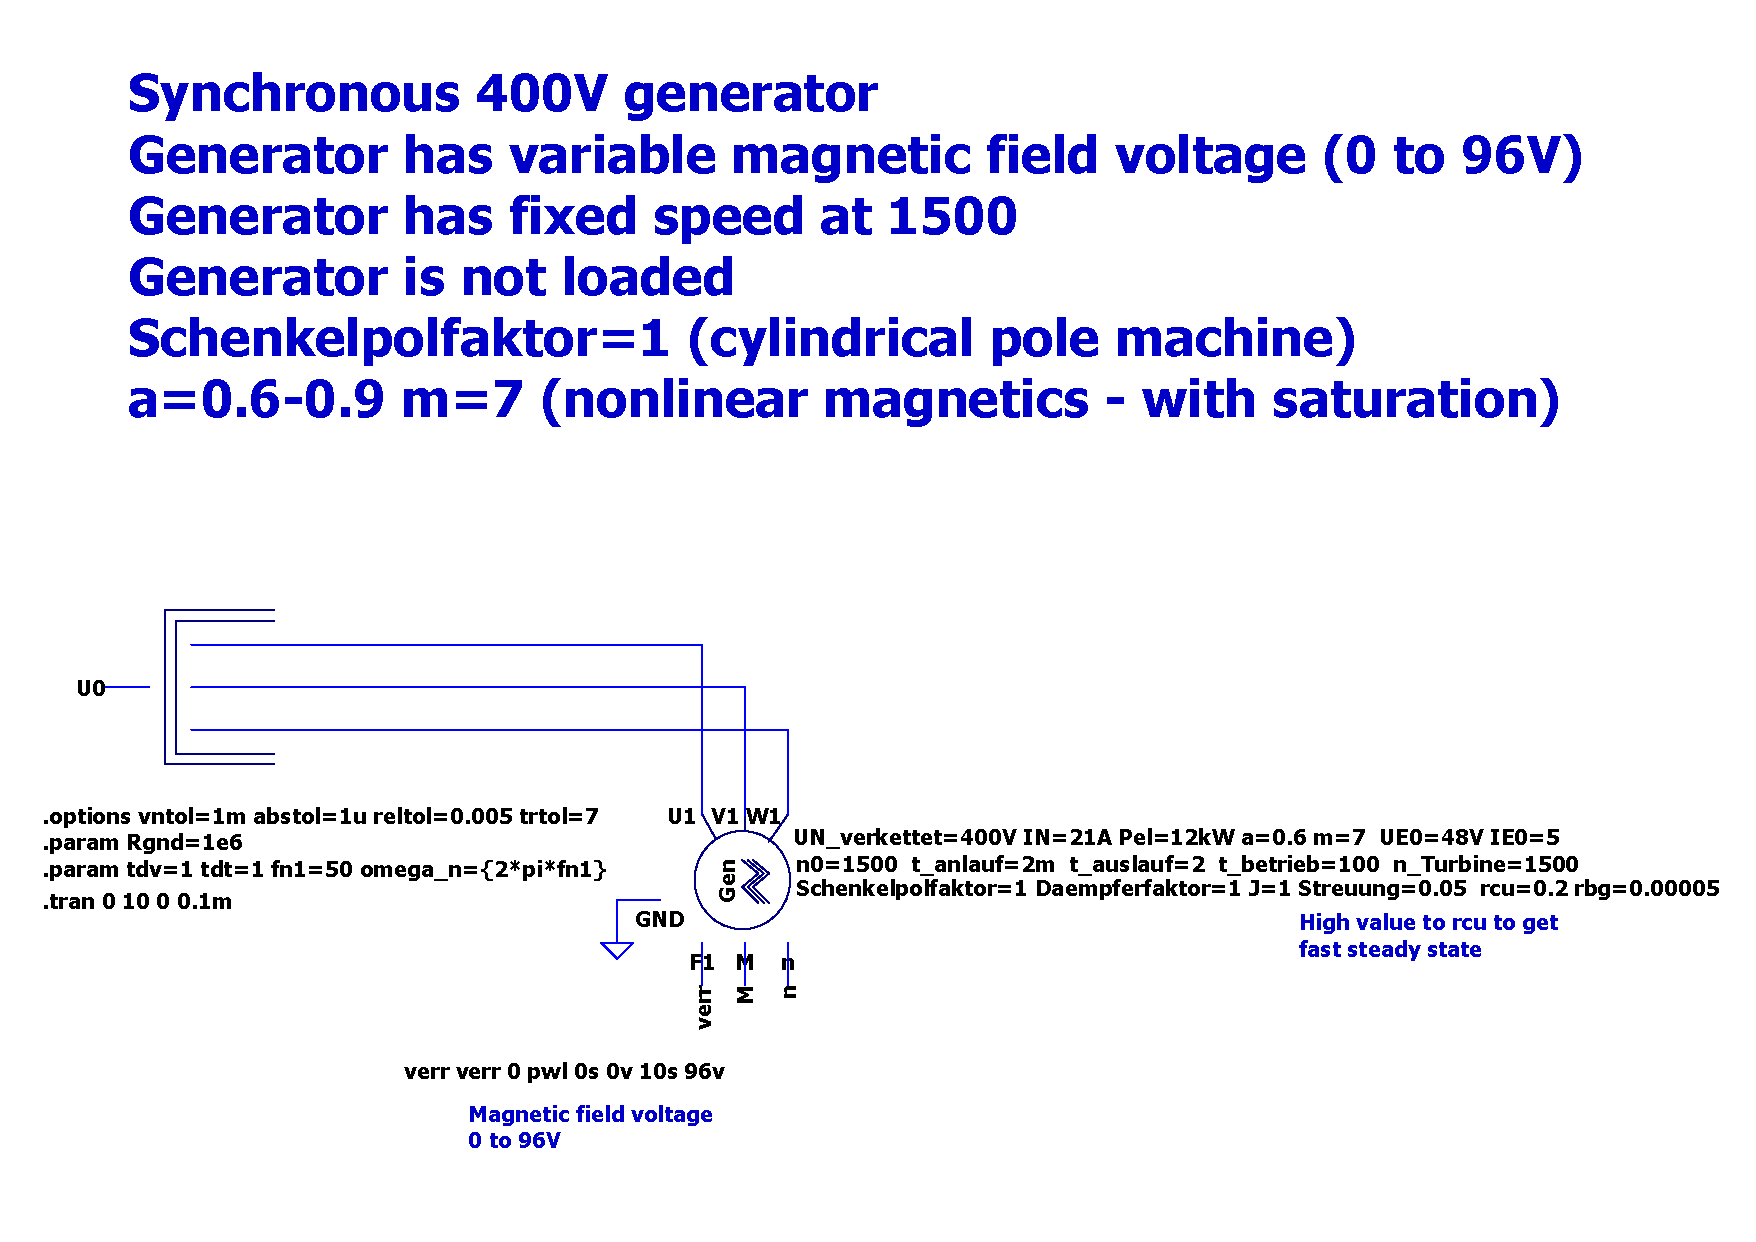
\includegraphics[width=1\textwidth] {figures/09_Synchronous_Generator_Characteristic_Curves_400V/sgen_400v_NoLoadLine_schematic.pdf}
	\caption{Open circuit characteristic - Schematic}
	\label{fig:figure91}
\end{figure}

\begin{figure}[H]
	\centering
	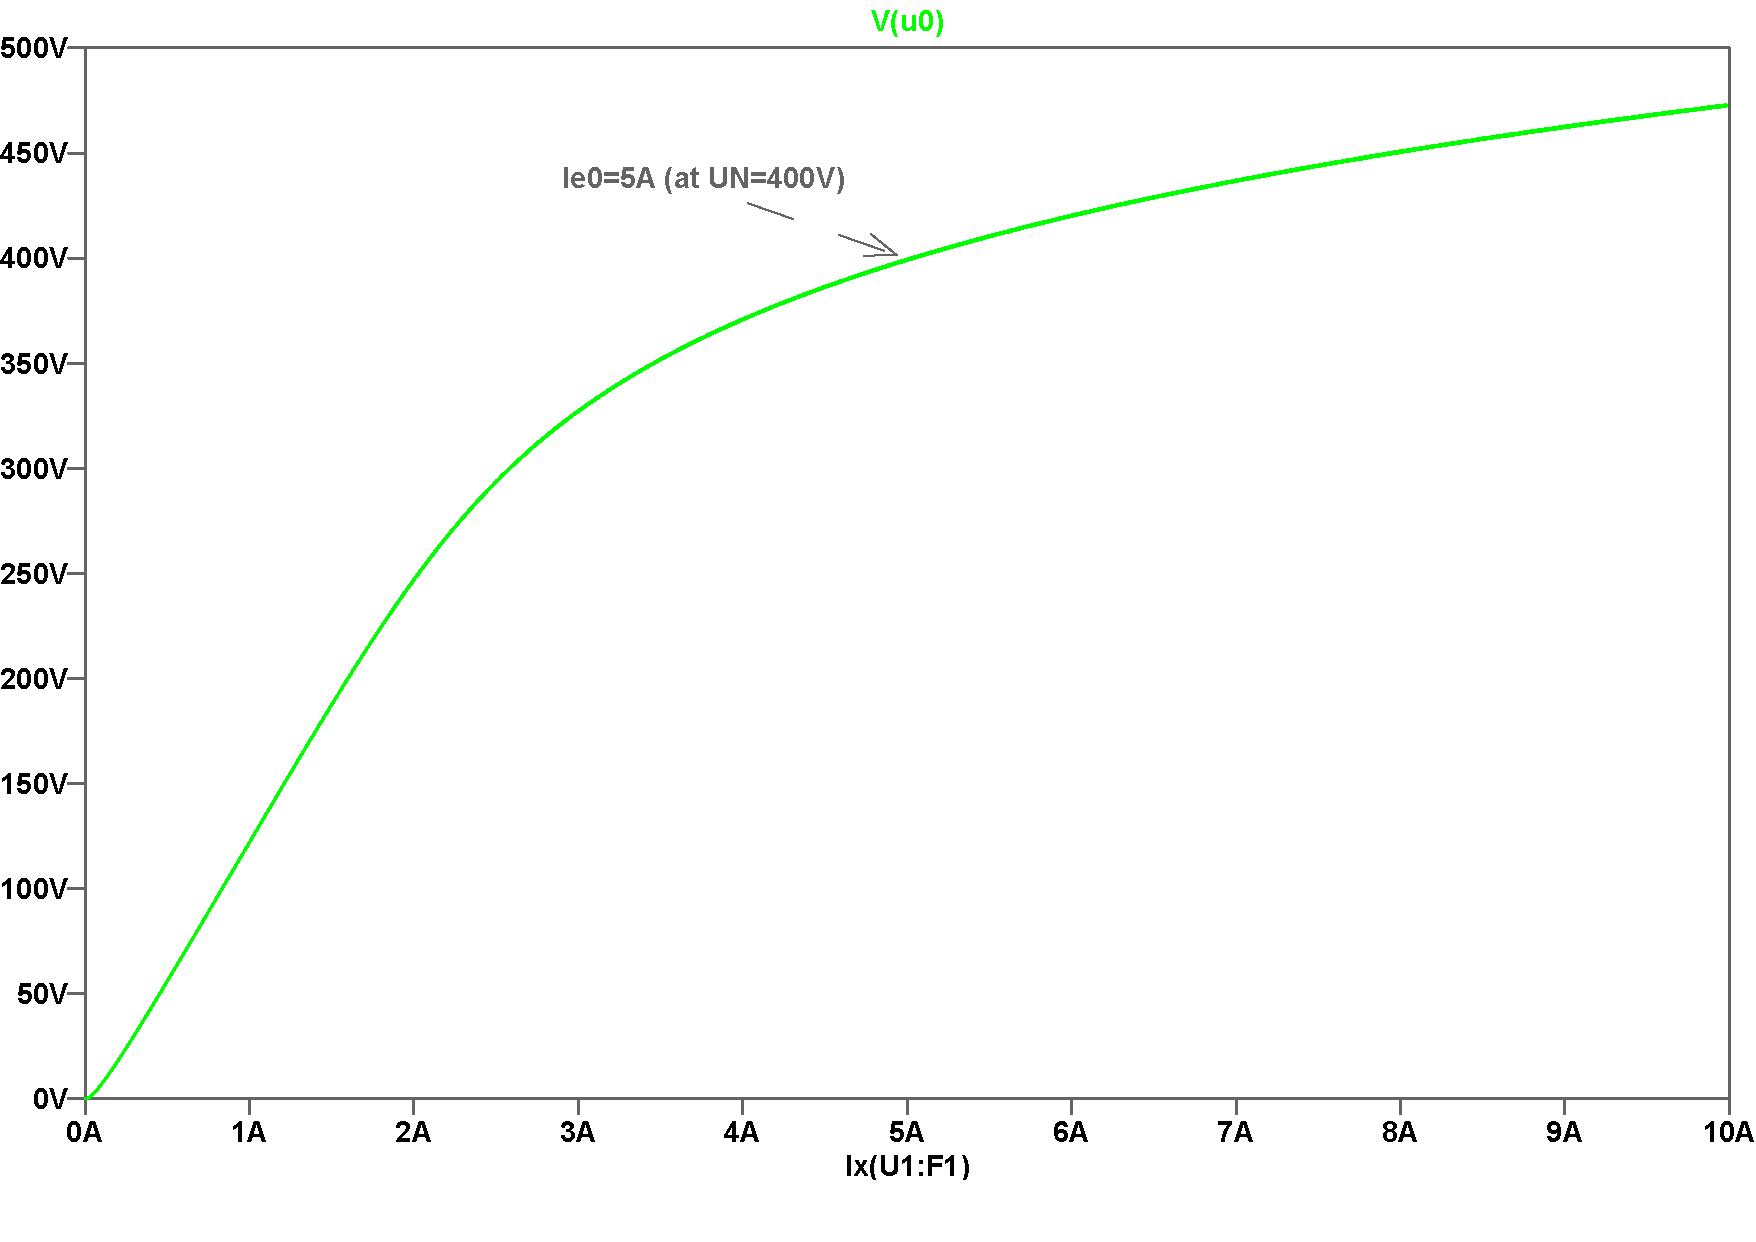
\includegraphics[width=0.9\textwidth] {figures/09_Synchronous_Generator_Characteristic_Curves_400V/sgen_400v_NoLoadLine_waveform.pdf}
	\caption{Open circuit characteristic - Waveform}
	\label{fig:figure92}
\end{figure}

\begin{itemize}
	\item determine the field current required for rated no-load voltage,
	\item investigate magnetic saturation and remanence,
	\item establish the air-gap line,
	\item estimate synchronous reactance and voltage regulation,
	\item determine the short-circuit ratio,
	\item select the operating range of the excitation system and AVR, and
	\item validate the saturation curve of a simulation model.
\end{itemize}

% ============================================================
\section{Short-Circuit Characteristic} see figure \ref{fig:figure93} and figure \ref{fig:figure94}  (simulation-file: same name as the heading) 
\label{sec:sg-scc}
% ============================================================

The short-circuit characteristic (SCC) describes the relationship between the
steady-state stator short-circuit current and the field current:

\begin{equation}
  I_k=f(I_f),
  \qquad U_s=0,
  \qquad n=n_N.
  \label{eq:sg-scc-definition}
\end{equation}

\subsection{Test Procedure}

The three stator terminals are short-circuited symmetrically through suitable
measuring equipment. The generator is driven at rated speed, and the
excitation is increased slowly from a small initial value. The corresponding
steady-state stator current is measured at each field-current setting.

\begin{important}{Current limitation during the test}{imp:sg-scc-safety}
The field current must be increased carefully. Rated stator current can be
reached at a field current considerably lower than that required for rated
open-circuit voltage. The conventional SCC test is normally stopped when the
rated stator current has been obtained.
\end{important}

\subsection{Shape of the Curve}

The short-circuit characteristic is approximately linear:

\begin{equation}
  I_k\propto I_f.
\end{equation}

During a symmetrical terminal short circuit, the terminal voltage is nearly
zero. The internal generated voltage is therefore balanced mainly by the
voltage drop across the synchronous impedance:

\begin{equation}
  \underline{E}
  \approx
  \left(R_s+\imag X_s\right)\underline{I}_k.
  \label{eq:sg-scc-phasor}
\end{equation}

Since normally $X_s\gg R_s$, the magnitude can be approximated by

\begin{equation}
  E\approx X_s I_k.
\end{equation}

The armature reaction is strongly demagnetizing during the symmetrical short
circuit. The resulting air-gap flux therefore remains comparatively small,
even when the stator current is high. The magnetic circuit operates mainly in
its unsaturated region, which explains the almost straight SCC.

\begin{figure}[H]
	\centering
	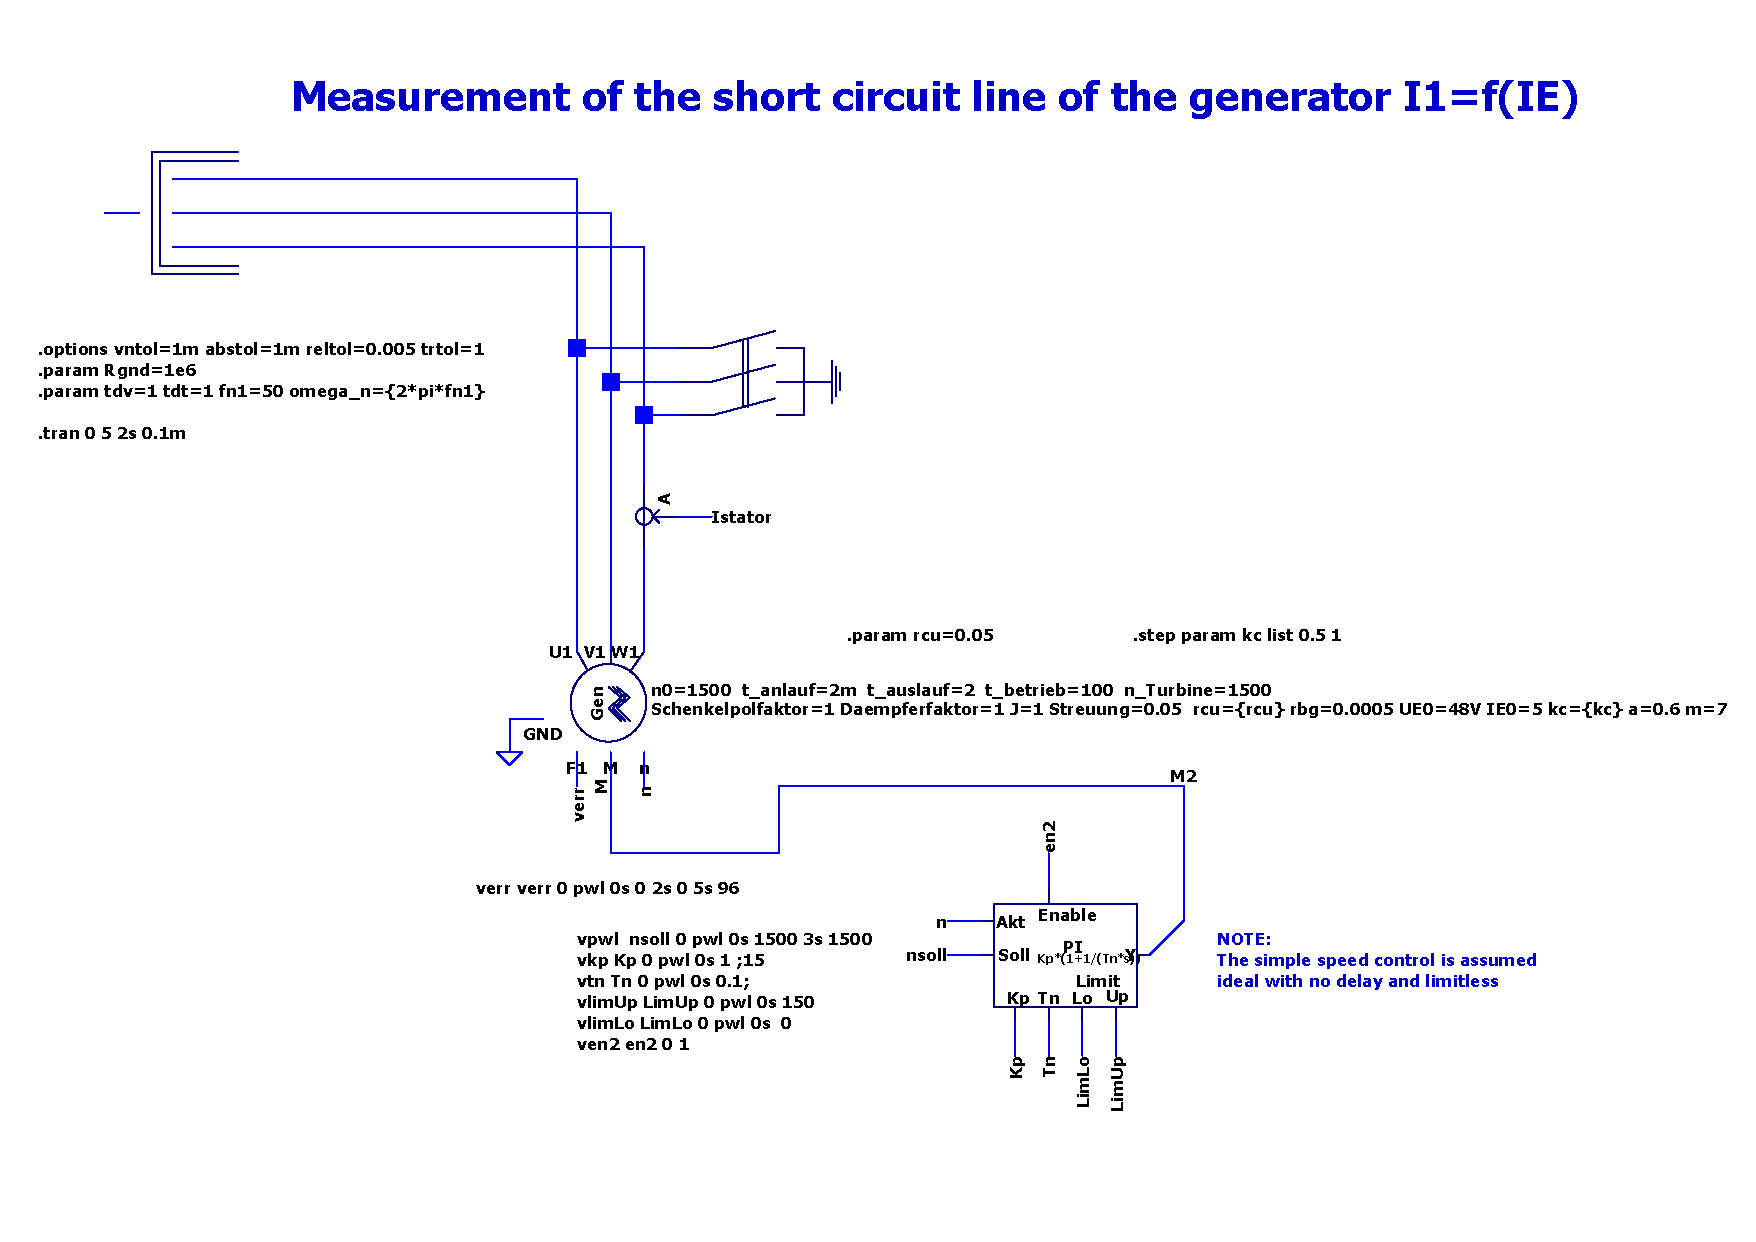
\includegraphics[width=0.9\textwidth] {figures/09_Synchronous_Generator_Characteristic_Curves_400V/sgen_400v_ShortCircuitLine_schematic.pdf}
	\caption{Short circuit characteristic - Schematic}
	\label{fig:figure93}
\end{figure}

\begin{figure}[H]
	\centering
	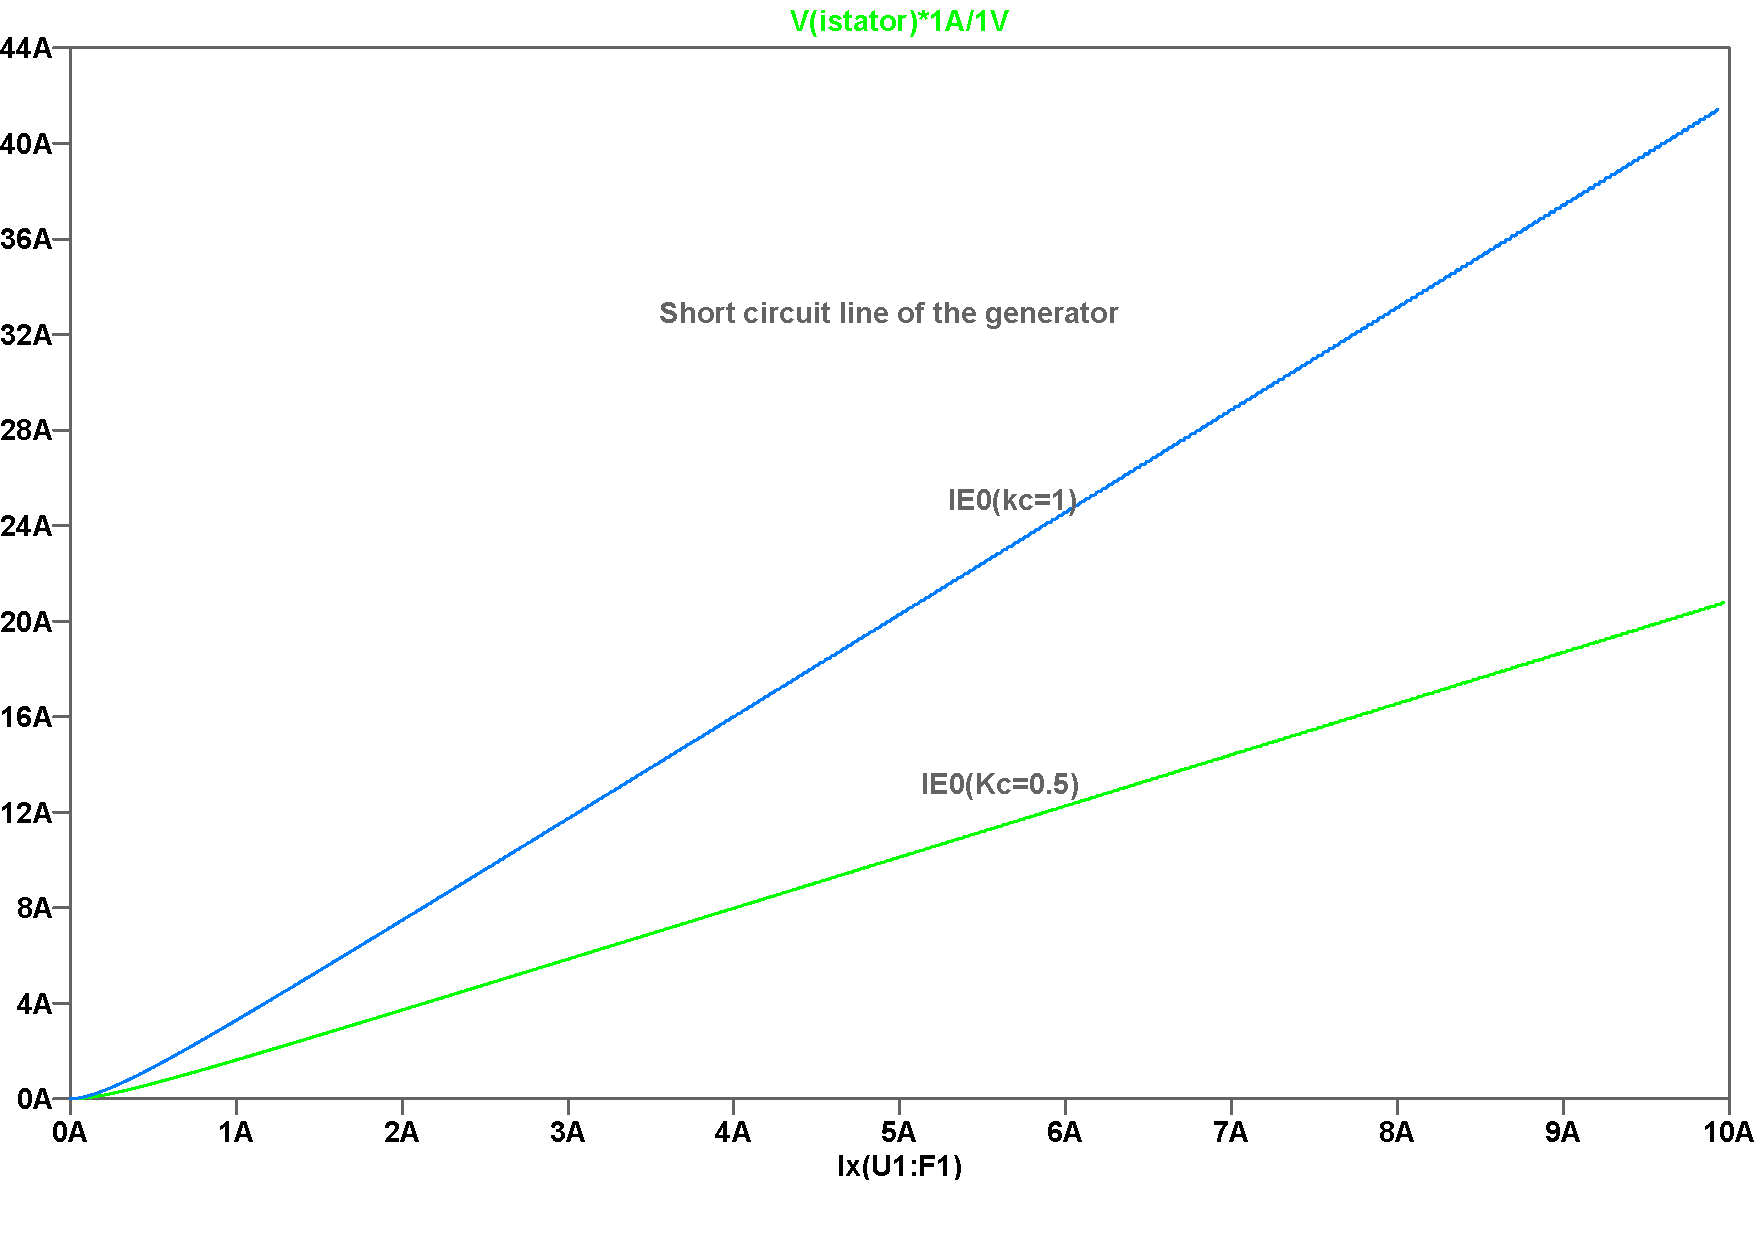
\includegraphics[width=0.9\textwidth] {figures/09_Synchronous_Generator_Characteristic_Curves_400V/sgen_400v_ShortCircuitLine_waveform.pdf}
	\caption{Short circuit characteristic - Waveform}
	\label{fig:figure94}
\end{figure}

The OCC is used to:


\subsection{Steady-State and Transient Short-Circuit Currents}

The conventional SCC represents the \emph{steady-state} short-circuit current.
Immediately after a sudden fault, however, the current is considerably higher
and passes through subtransient, transient, and steady-state intervals.

Neglecting resistance and using the appropriate direct-axis reactances, the
symmetrical AC components can be estimated as

\begin{align}
  I_k'' &\approx \frac{E}{X_d''},
  & \text{subtransient current}, \\
  I_k'  &\approx \frac{E}{X_d'},
  & \text{transient current}, \\
  I_k   &\approx \frac{E}{X_d},
  & \text{steady-state current}.
  \label{eq:sg-fault-current-stages}
\end{align}

The first interval is dominated by the stator and damper-winding flux
constraints. After the damper currents decay, the transient reactance becomes
effective. Finally, after the field transient has decayed, the current is
determined mainly by the synchronous reactance.

\begin{remark}{Sudden-fault waveform}{rem:sg-scc-transient}
The actual phase current following a sudden short circuit may also contain a
decaying DC component. Its magnitude depends on the fault inception angle and
the pre-fault operating point. The peak phase current can therefore be much
larger than the symmetrical RMS current represented by the SCC.
\end{remark}

\subsection{Synchronous-Impedance Estimate}

The OCC and SCC can be combined to estimate the synchronous impedance. The
open-circuit voltage and short-circuit current must be evaluated at the same
field current.

\begin{calculation}{Synchronous impedance from OCC and SCC}{calc:sg-zs-occ-scc}
Using phase voltage and phase current,
\begin{align}
  Z_s &= \frac{U_{0,\mathrm{ph}}}{I_k}, \\
  X_s &= \sqrt{Z_s^2-R_s^2}.
\end{align}

If the stator resistance is small compared with the reactance,
\begin{equation}
  X_s\approx Z_s.
\end{equation}
\end{calculation}

The OCC may already be saturated at the selected field current, whereas the
SCC remains almost unsaturated. The synchronous-impedance method therefore
usually gives a conservative, relatively high estimate of voltage regulation.

\subsection{Short-Circuit Ratio}

The short-circuit ratio is commonly defined as

\begin{equation}
  \mathrm{SCR}
  =\frac{I_{f,U_N}}{I_{f,I_N}},
  \label{eq:sg-scr}
\end{equation}

where $I_{f,U_N}$ is the field current required to produce rated voltage on
open circuit and $I_{f,I_N}$ is the field current required to produce rated
stator current under steady-state short-circuit conditions. Approximately,

\begin{equation}
  \mathrm{SCR}\approx\frac{1}{x_d},
\end{equation}

when $x_d$ is expressed in per unit. Saturation and the exact test definition
affect this relationship.

A comparatively large SCR generally indicates a smaller synchronous
reactance, improved steady-state voltage regulation, and a larger stability
margin. It also leads to higher short-circuit current and usually requires a
physically larger and more expensive machine.

\newpage

% ============================================================
\section{Load or External Characteristic} see figure \ref{fig:figure95}-\ref{fig:figure910}  (simulation-files: same names as the headings) 
\label{sec:sg-load-characteristic}
% ============================================================

The load characteristic describes how the generator terminal voltage changes
with stator current when speed, field current, and load power factor remain
constant:

\begin{equation}
  U=f(I_s),
  \qquad
  n=\text{constant},
  \qquad
  I_f=\text{constant},
  \qquad
  \cos\varphi=\text{constant}.
  \label{eq:sg-load-characteristic}
\end{equation}

It is therefore also called the \emph{external characteristic} of the
generator.

For a simplified round-rotor generator, the steady-state phasor equation is

\begin{equation}
  \underline{E}
  =\underline{U}
  +\left(R_s+\imag X_s\right)\underline{I}_s.
  \label{eq:sg-generator-phasor}
\end{equation}

If field current and speed are constant, the magnitude of $E$ is approximately
constant. The terminal voltage must consequently change when the stator current
changes. The direction and magnitude of this voltage change depend strongly on
the load power factor.

\subsection{Inductive Load}

For a lagging load, the stator current lags behind the terminal voltage. The
reactive voltage drop $\imag X_s\underline{I}_s$ and the demagnetizing armature
reaction reduce the terminal voltage. Consequently, the voltage falls
significantly as the load current rises, and the external characteristic has a
pronounced negative slope.

\subsection{Unity-Power-Factor Load}

At unity power factor, stator current and terminal voltage are in phase. The
terminal voltage still decreases as the current increases, but usually less
strongly than for an inductive load. The reduction results from stator
resistance, synchronous reactance, armature reaction, and magnetic saturation.

\subsection{Capacitive Load}

For a leading load, the stator current leads the terminal voltage. The armature
reaction can then have a magnetizing effect. As the current increases, the
terminal voltage may remain nearly constant or even rise. The external
characteristic can therefore have a positive slope.

This behaviour explains why capacitive loads and overexcited synchronous
machines can support the voltage of a power system.


\subsection{Voltage Regulation}

The voltage regulation of a synchronous generator is commonly expressed as

\begin{equation}
  \varepsilon_U
  =\frac{U_0-U_N}{U_N}\cdot100\%,
  \label{eq:sg-voltage-regulation}
\end{equation}

where $U_0$ is the no-load voltage obtained after removing the load without
changing speed or field current, and $U_N$ is the terminal voltage at the
specified load.

For an inductive load, the regulation is normally positive because
$U_0>U_N$. For a sufficiently capacitive load, it may become negative because
the loaded terminal voltage can exceed the corresponding no-load voltage.

% ============================================================

\begin{figure}[H]
	\centering
	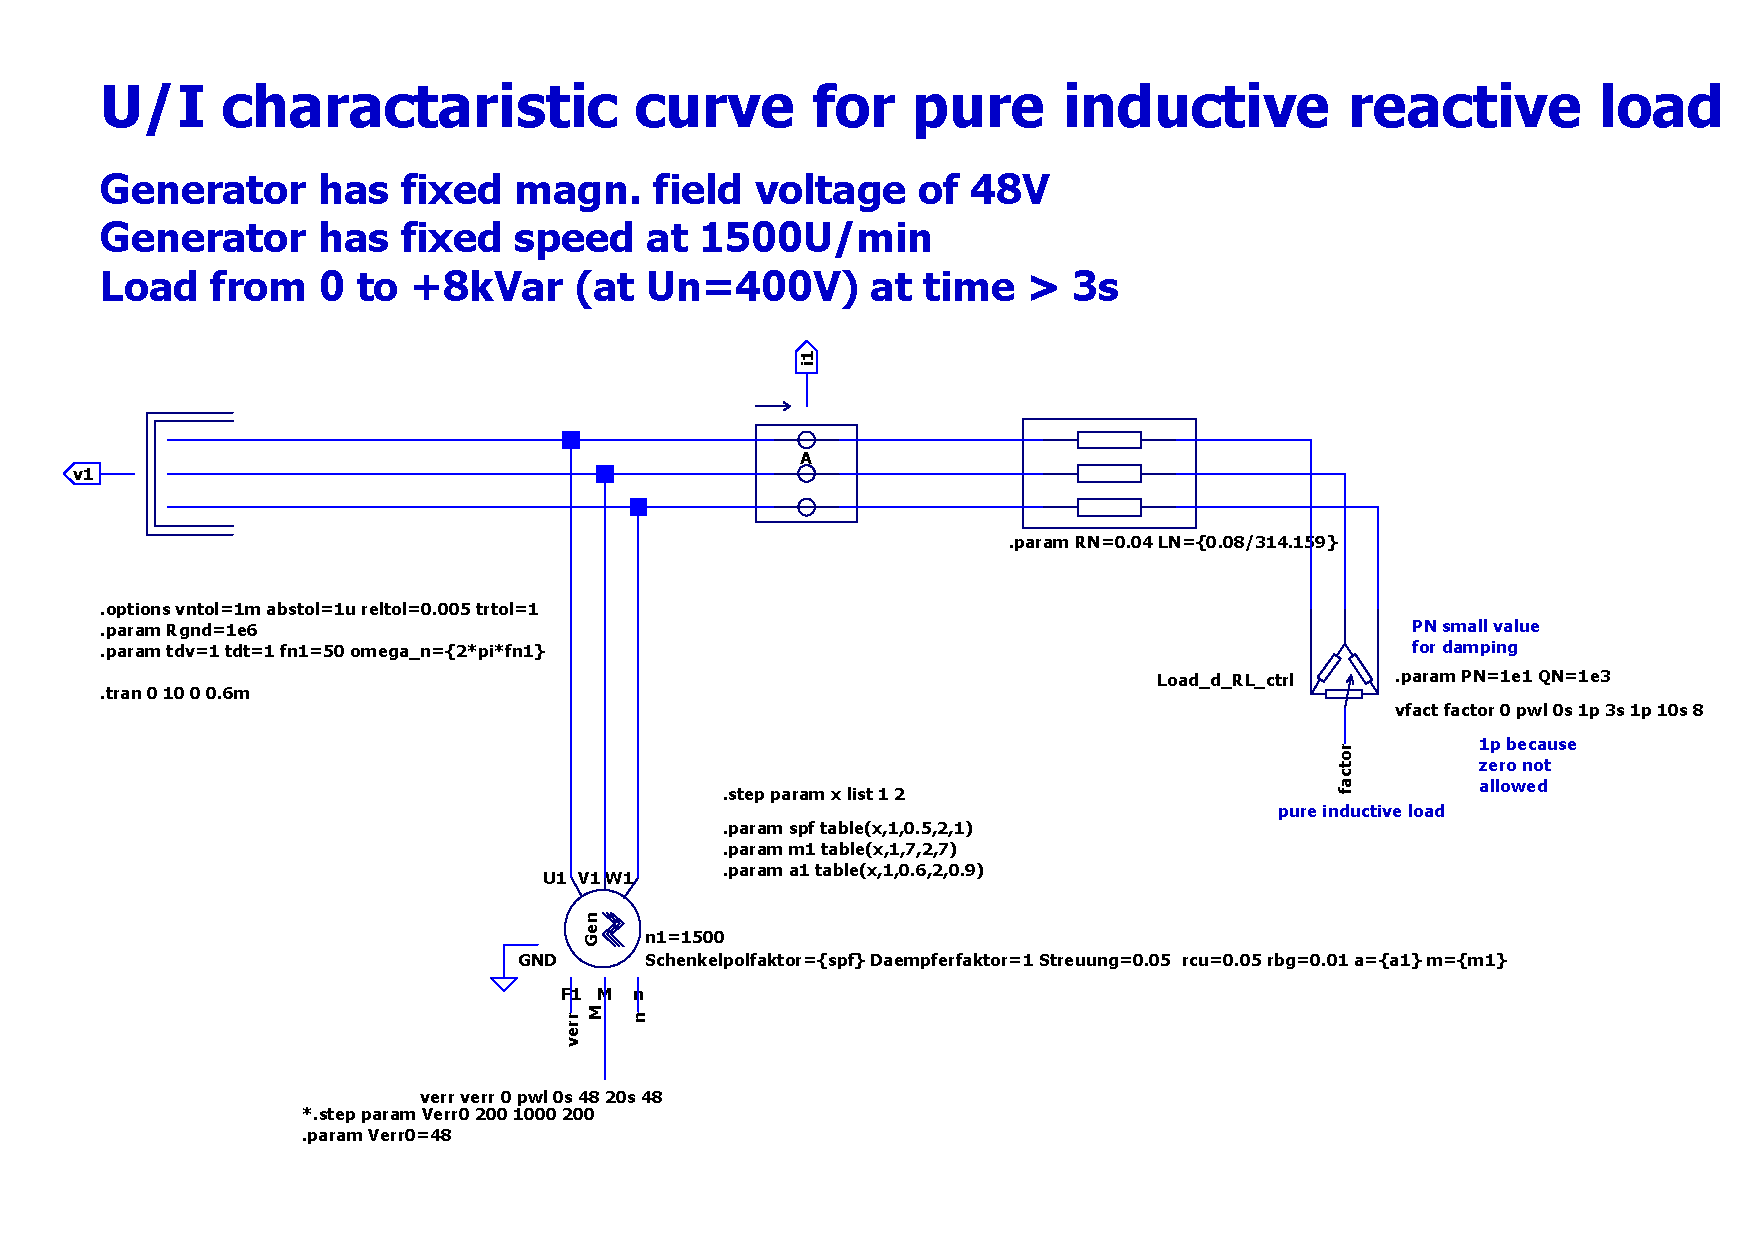
\includegraphics[width=0.9\textwidth] {figures/09_Synchronous_Generator_Characteristic_Curves_400V/sgen_400v_constant_speed_loadcurve_induktiv_schematic.pdf}
	\caption{Inductive characteristic - Schematic}
	\label{fig:figure95}
\end{figure}

\begin{figure}[H]
	\centering
	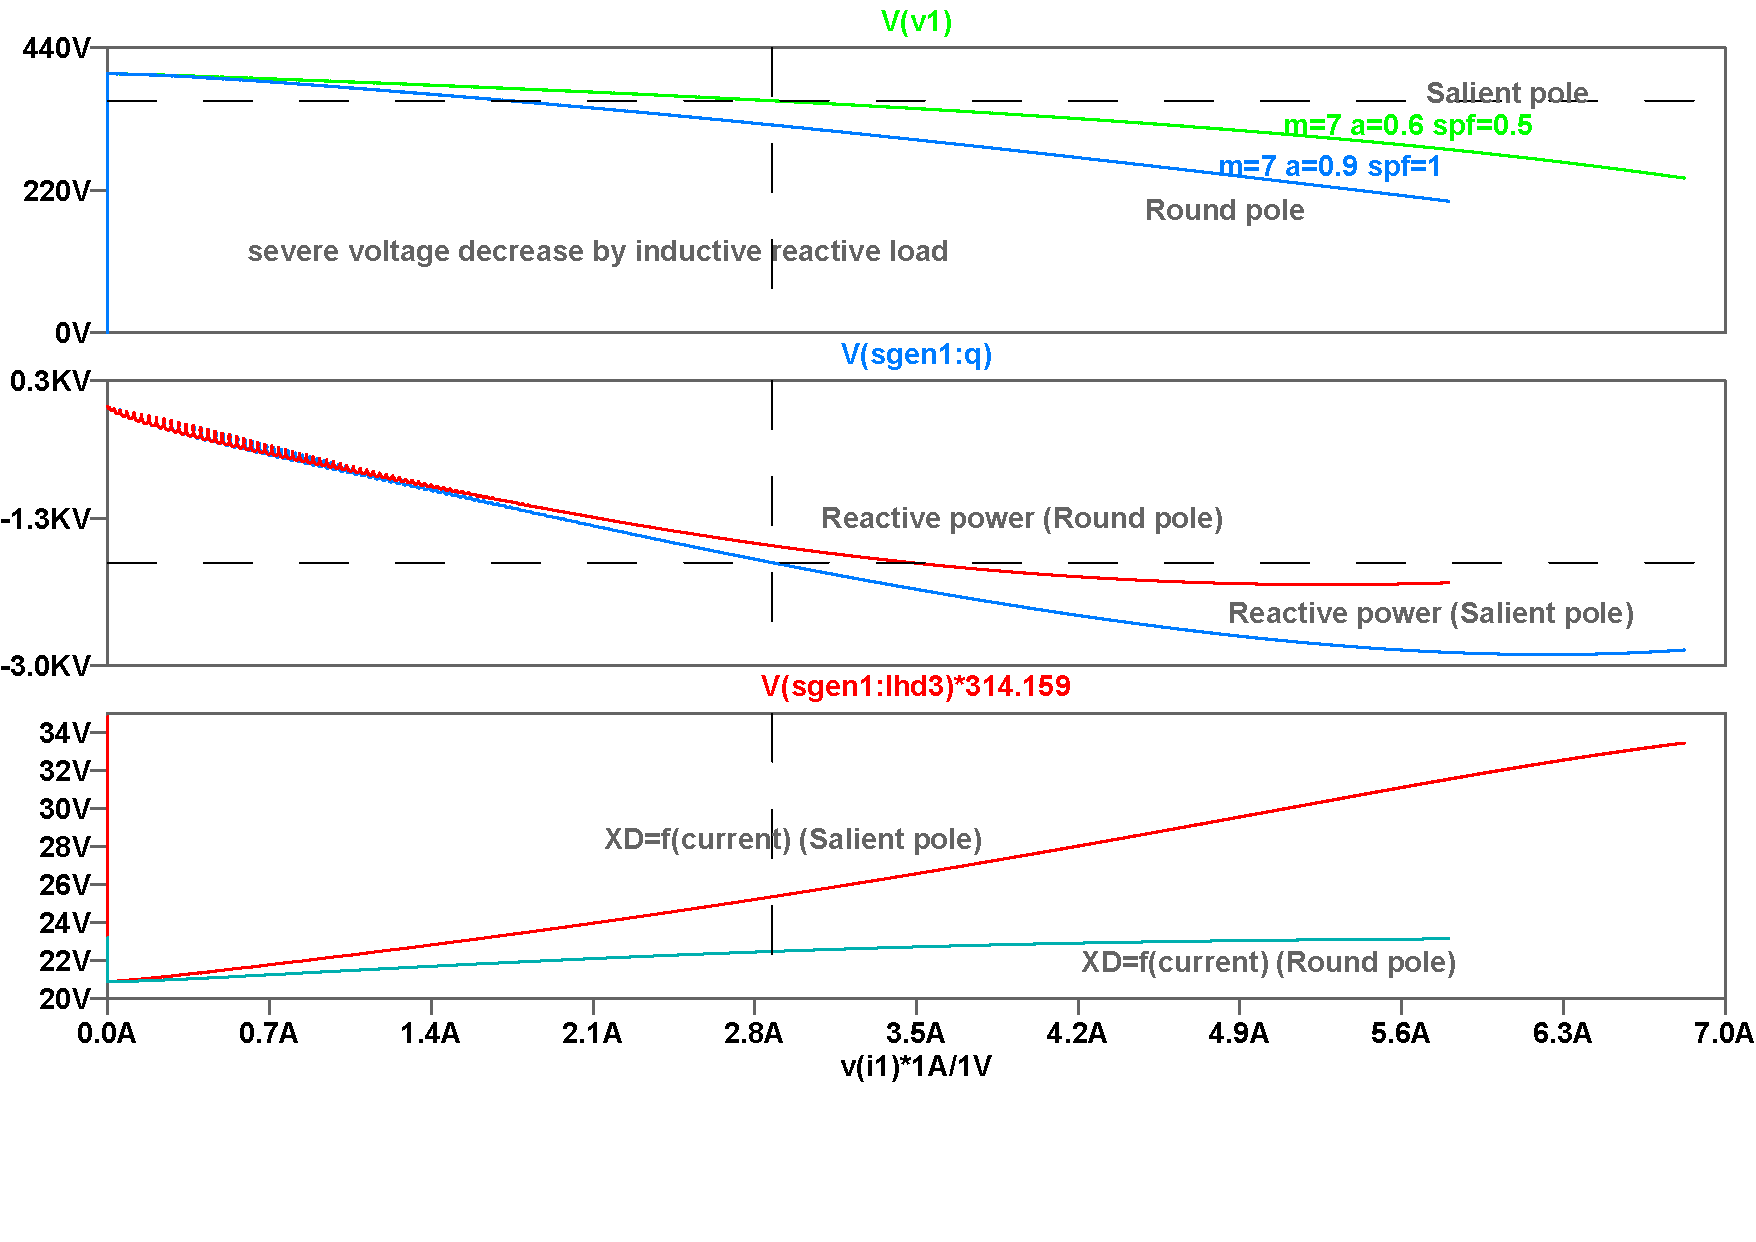
\includegraphics[width=0.9\textwidth] {figures/09_Synchronous_Generator_Characteristic_Curves_400V/sgen_400v_constant_speed_loadcurve_induktiv_waveform.pdf}
	\caption{Inductive characteristic - Waveform}
	\label{fig:figure96}
\end{figure}

\begin{figure}[H]
	\centering
	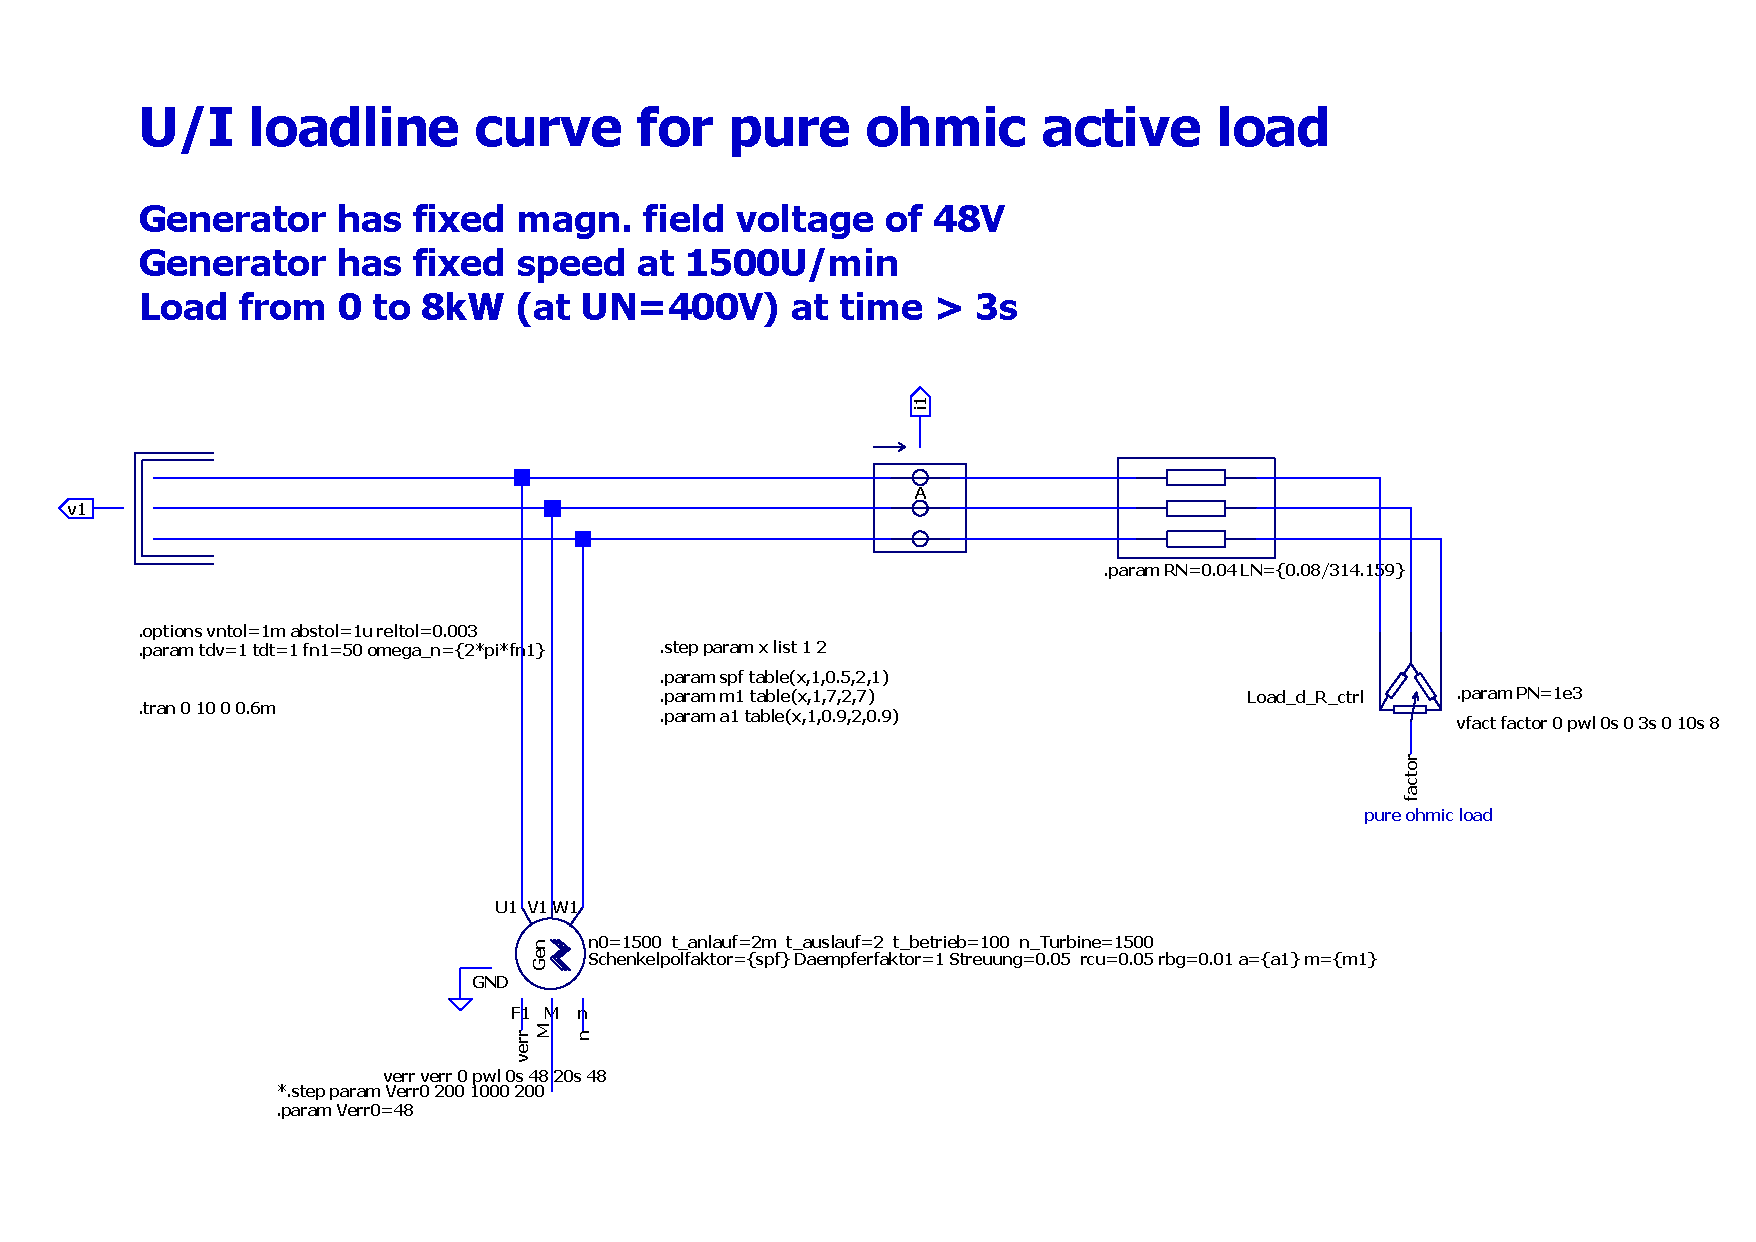
\includegraphics[width=0.9\textwidth] {figures/09_Synchronous_Generator_Characteristic_Curves_400V/sgen_400v_constant_speed_loadcurve_ohmic_schematic.pdf}
	\caption{Resistive characteristic - Schematic}
	\label{fig:figure97}
\end{figure}

\begin{figure}[H]
	\centering
	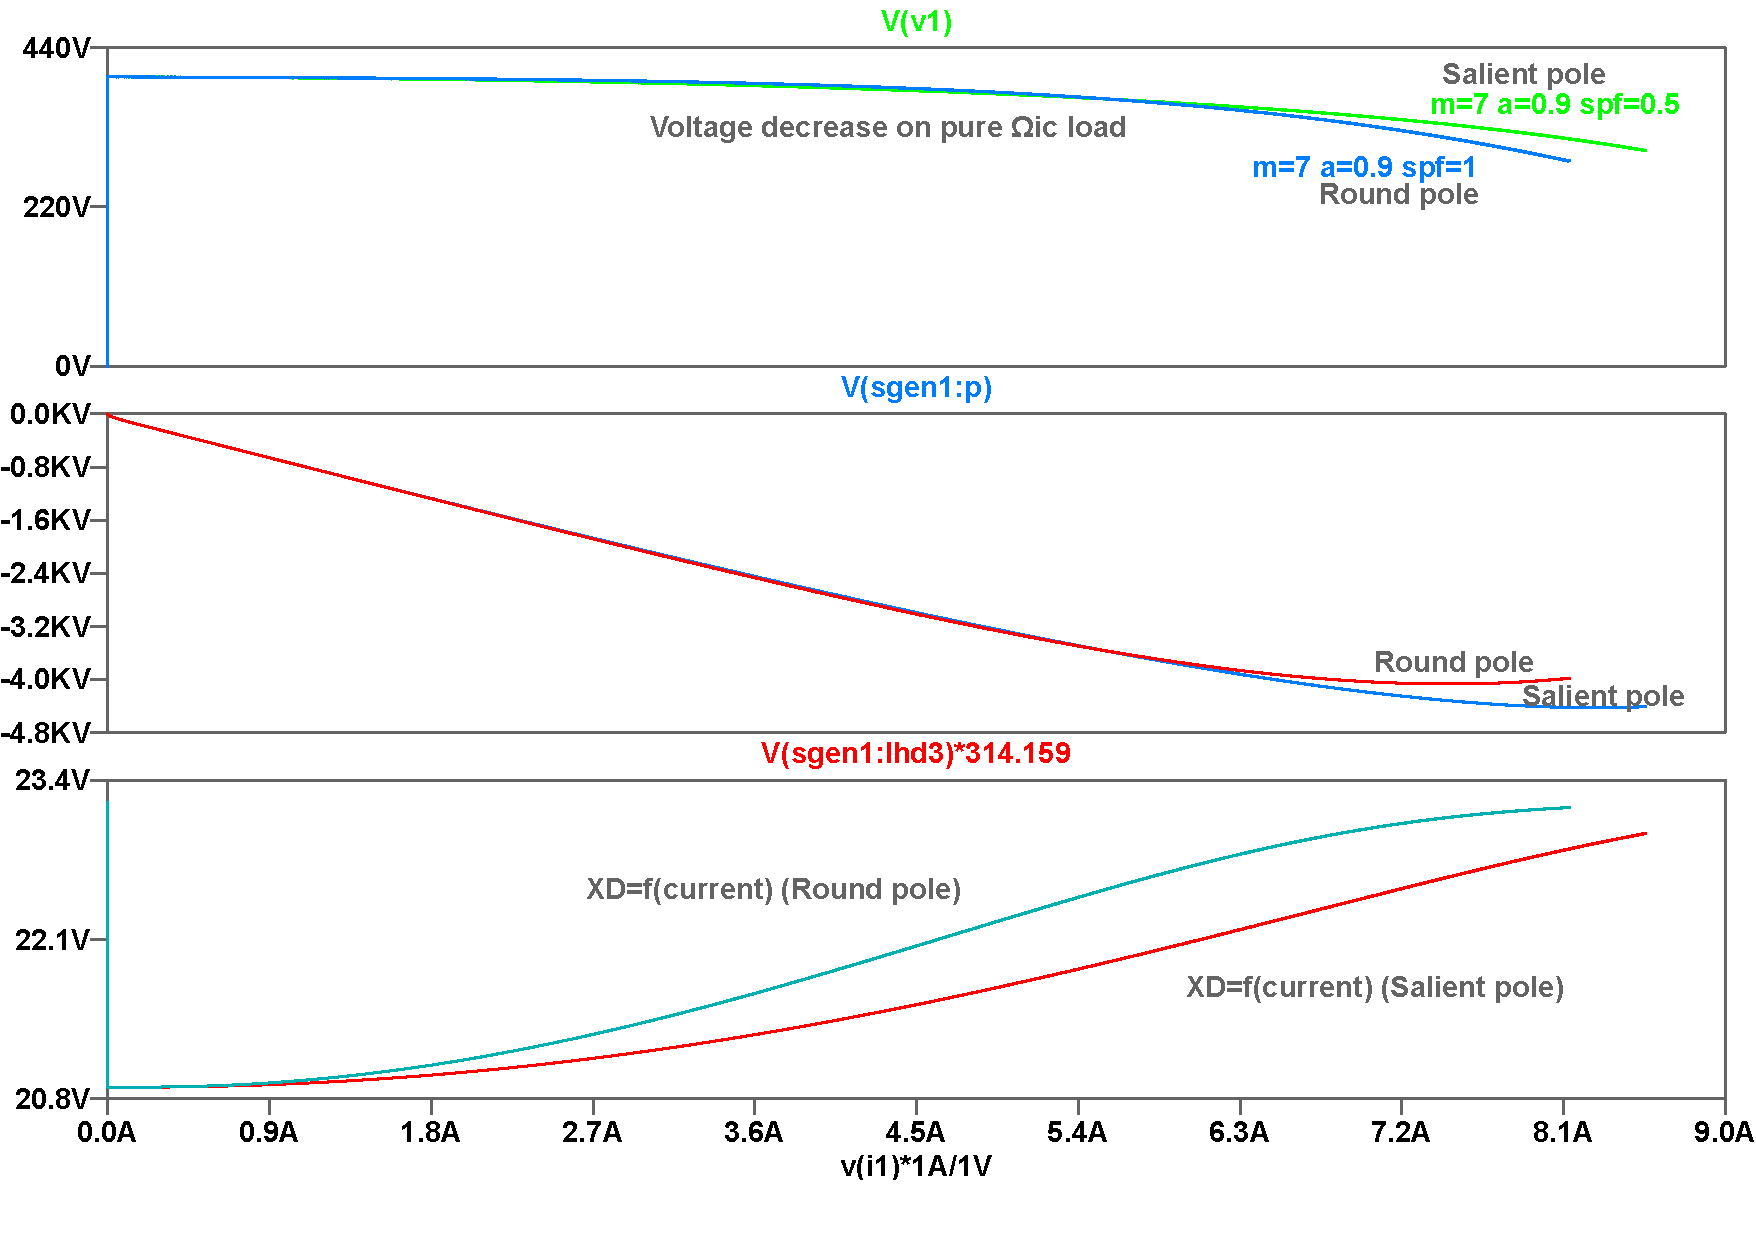
\includegraphics[width=0.9\textwidth] {figures/09_Synchronous_Generator_Characteristic_Curves_400V/sgen_400v_constant_speed_loadcurve_ohmic_waveform.pdf}
	\caption{Resistive characteristic - Waveform}
	\label{fig:figure98}
\end{figure}

\begin{figure}[H]
	\centering
	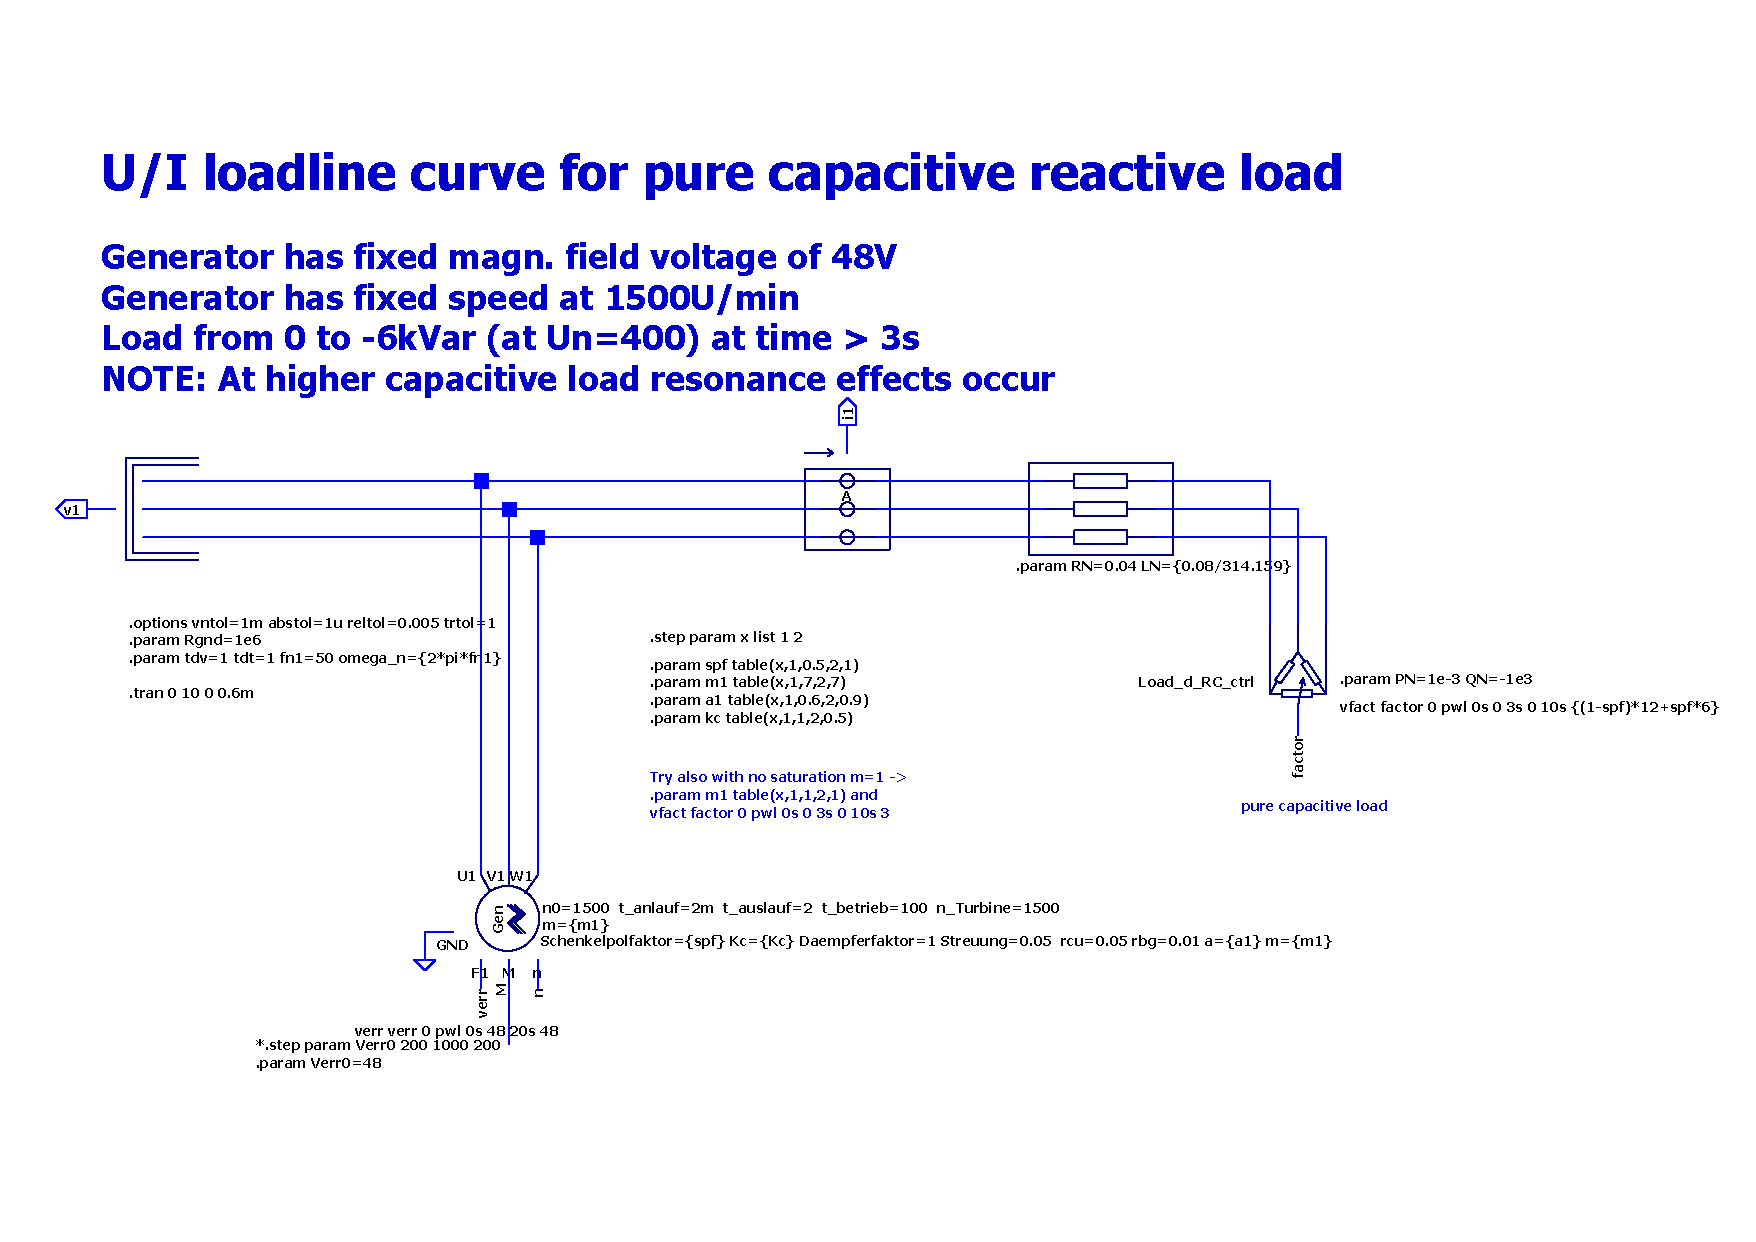
\includegraphics[width=0.9\textwidth] {figures/09_Synchronous_Generator_Characteristic_Curves_400V/sgen_400v_constant_speed_loadcurve_capacitive_schematic.pdf}
	\caption{Capacitive characteristic - Schematic}
	\label{fig:figure99}
\end{figure}

\begin{figure}[H]
	\centering
	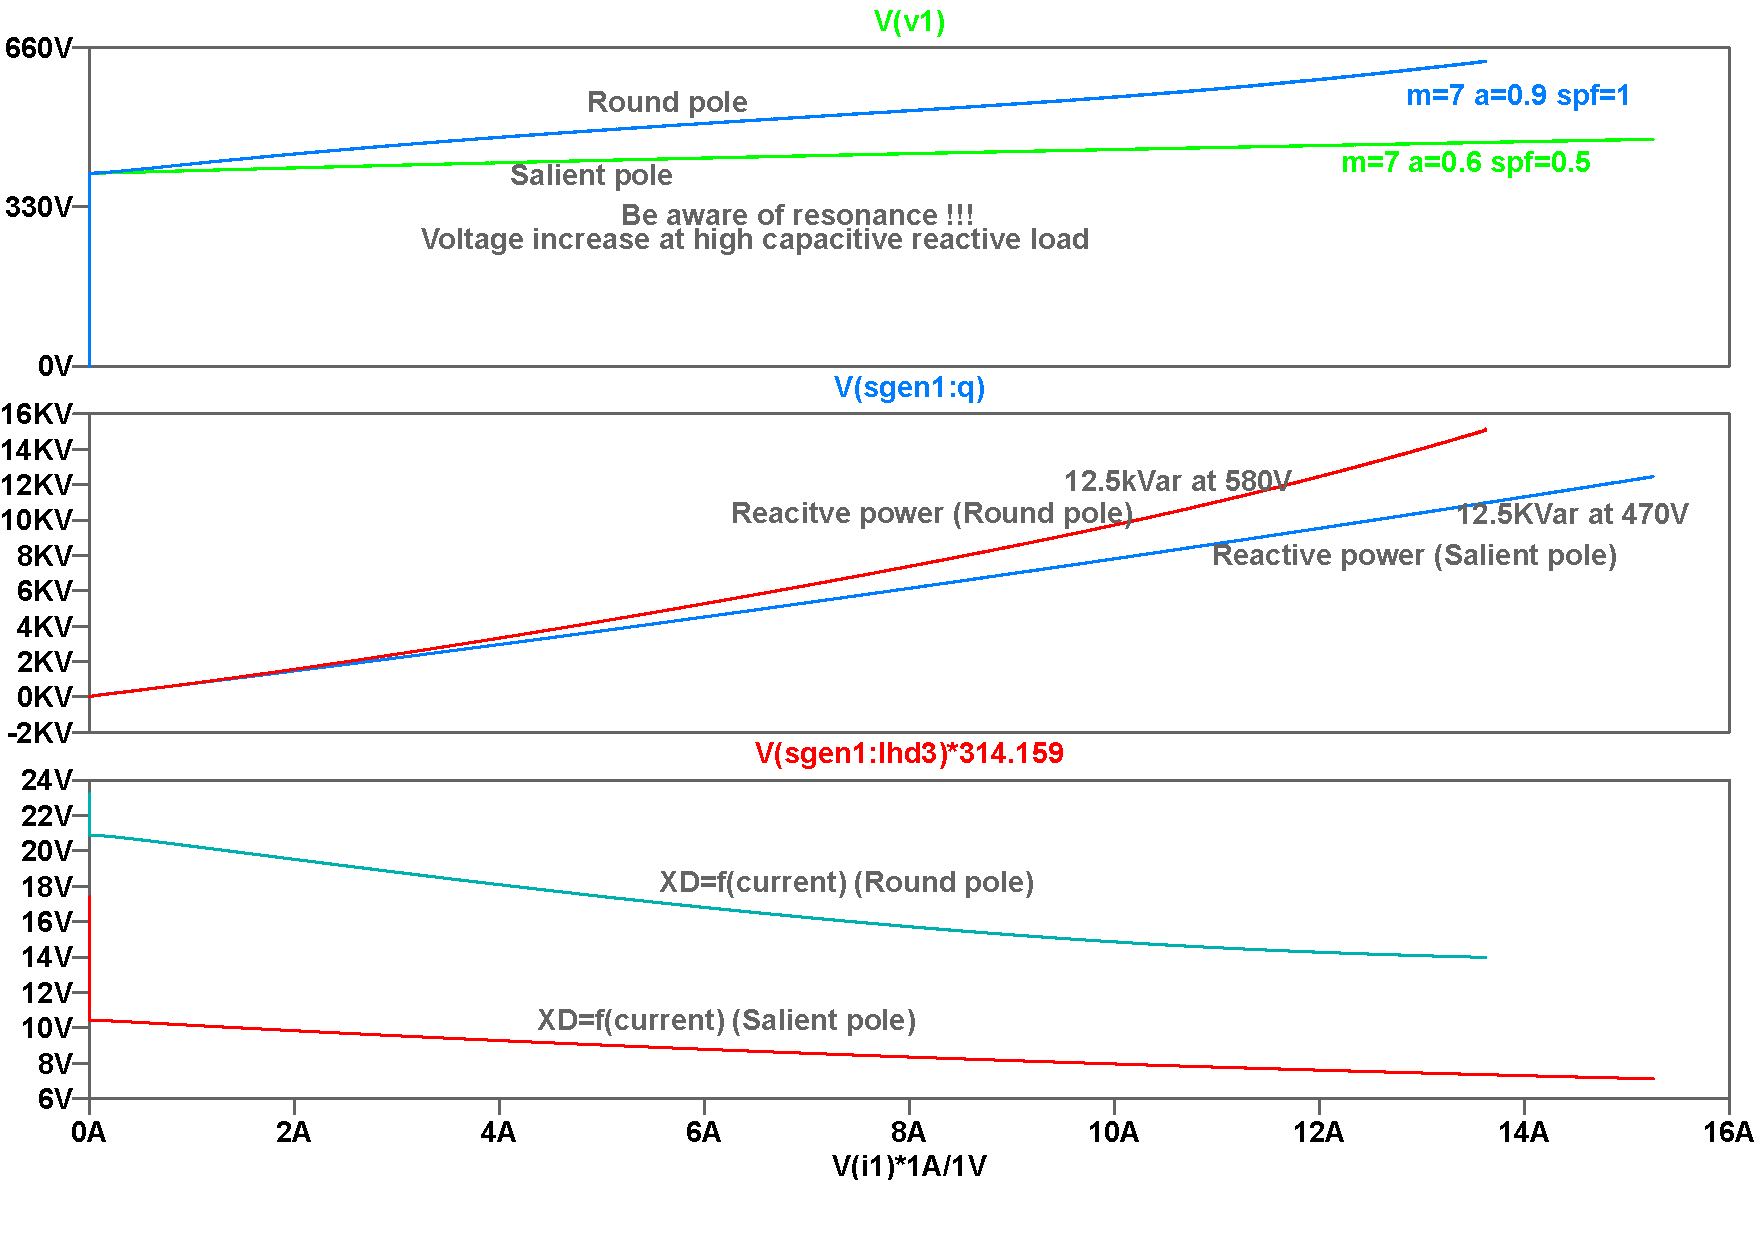
\includegraphics[width=0.9\textwidth] {figures/09_Synchronous_Generator_Characteristic_Curves_400V/sgen_400v_constant_speed_loadcurve_capacitive_waveform.pdf}
	\caption{Capacitive characteristic - Waveform}
	\label{fig:figure910}
\end{figure}

\section{Regulation Characteristic} see figures \ref{fig:figure911}-\ref{fig:figure916}  (simulation-file: same names as the headings) 
\label{sec:sg-regulation-characteristic}
% ============================================================

The regulation characteristic describes the field current required to
maintain constant terminal voltage while the stator current changes:

\begin{equation}
  I_f=f(I_s),
  \qquad
  U=U_N,
  \qquad
  n=n_N,
  \qquad
  \cos\varphi=\text{constant}.
  \label{eq:sg-regulation-characteristic}
\end{equation}

It is sometimes called the excitation characteristic under load.

\begin{important}{Difference between load and regulation characteristics}
  {imp:sg-load-versus-regulation}
The load characteristic gives $U=f(I_s)$ at constant excitation. The
regulation characteristic gives $I_f=f(I_s)$ while the terminal voltage is
kept constant. The two characteristics therefore describe complementary
operating conditions.
\end{important}

\subsection{Inductive Load}

For a lagging load, armature reaction is predominantly demagnetizing, and the
synchronous-reactance voltage drop increases with stator current. The
excitation must therefore be increased as the load rises:

\begin{equation}
  I_s\uparrow
  \quad\Longrightarrow\quad
  I_f\uparrow.
\end{equation}

The regulation curve consequently rises relatively steeply.

\subsection{Unity-Power-Factor Load}

At unity power factor, the required field current normally increases with
stator current, but less strongly than for an inductive load.

\subsection{Capacitive Load}

For a leading load, armature reaction is partly magnetizing. Less field current
is therefore required to maintain rated terminal voltage. Over part of the
operating range,

\begin{equation}
  I_s\uparrow
  \quad\Longrightarrow\quad
  I_f\downarrow.
\end{equation}

For strongly capacitive operating conditions, the generator may therefore
have to operate underexcited.

\subsection{Practical Importance}

The regulation characteristic is directly related to the task of the AVR.
When load current and power factor change, the AVR adjusts field voltage and
field current so that the terminal voltage remains at its reference value.

%The characteristic is useful for:
%
%\begin{itemize}
%  \item selecting the required excitation-voltage and field-current range,
%  \item designing and limiting the AVR,
%  \item estimating reactive-power requirements,
%  \item checking rotor field-winding heating, and
%  \item determining permissible underexcited operation.
%\end{itemize}

%\begin{remark}{Static and dynamic regulation}{rem:sg-static-regulation}
%The regulation characteristic contains steady-state operating points. It does
%not describe the transient response, stability, or time constants of the AVR
%and excitation system.
%\end{remark}

\begin{figure}[H]
	\centering
	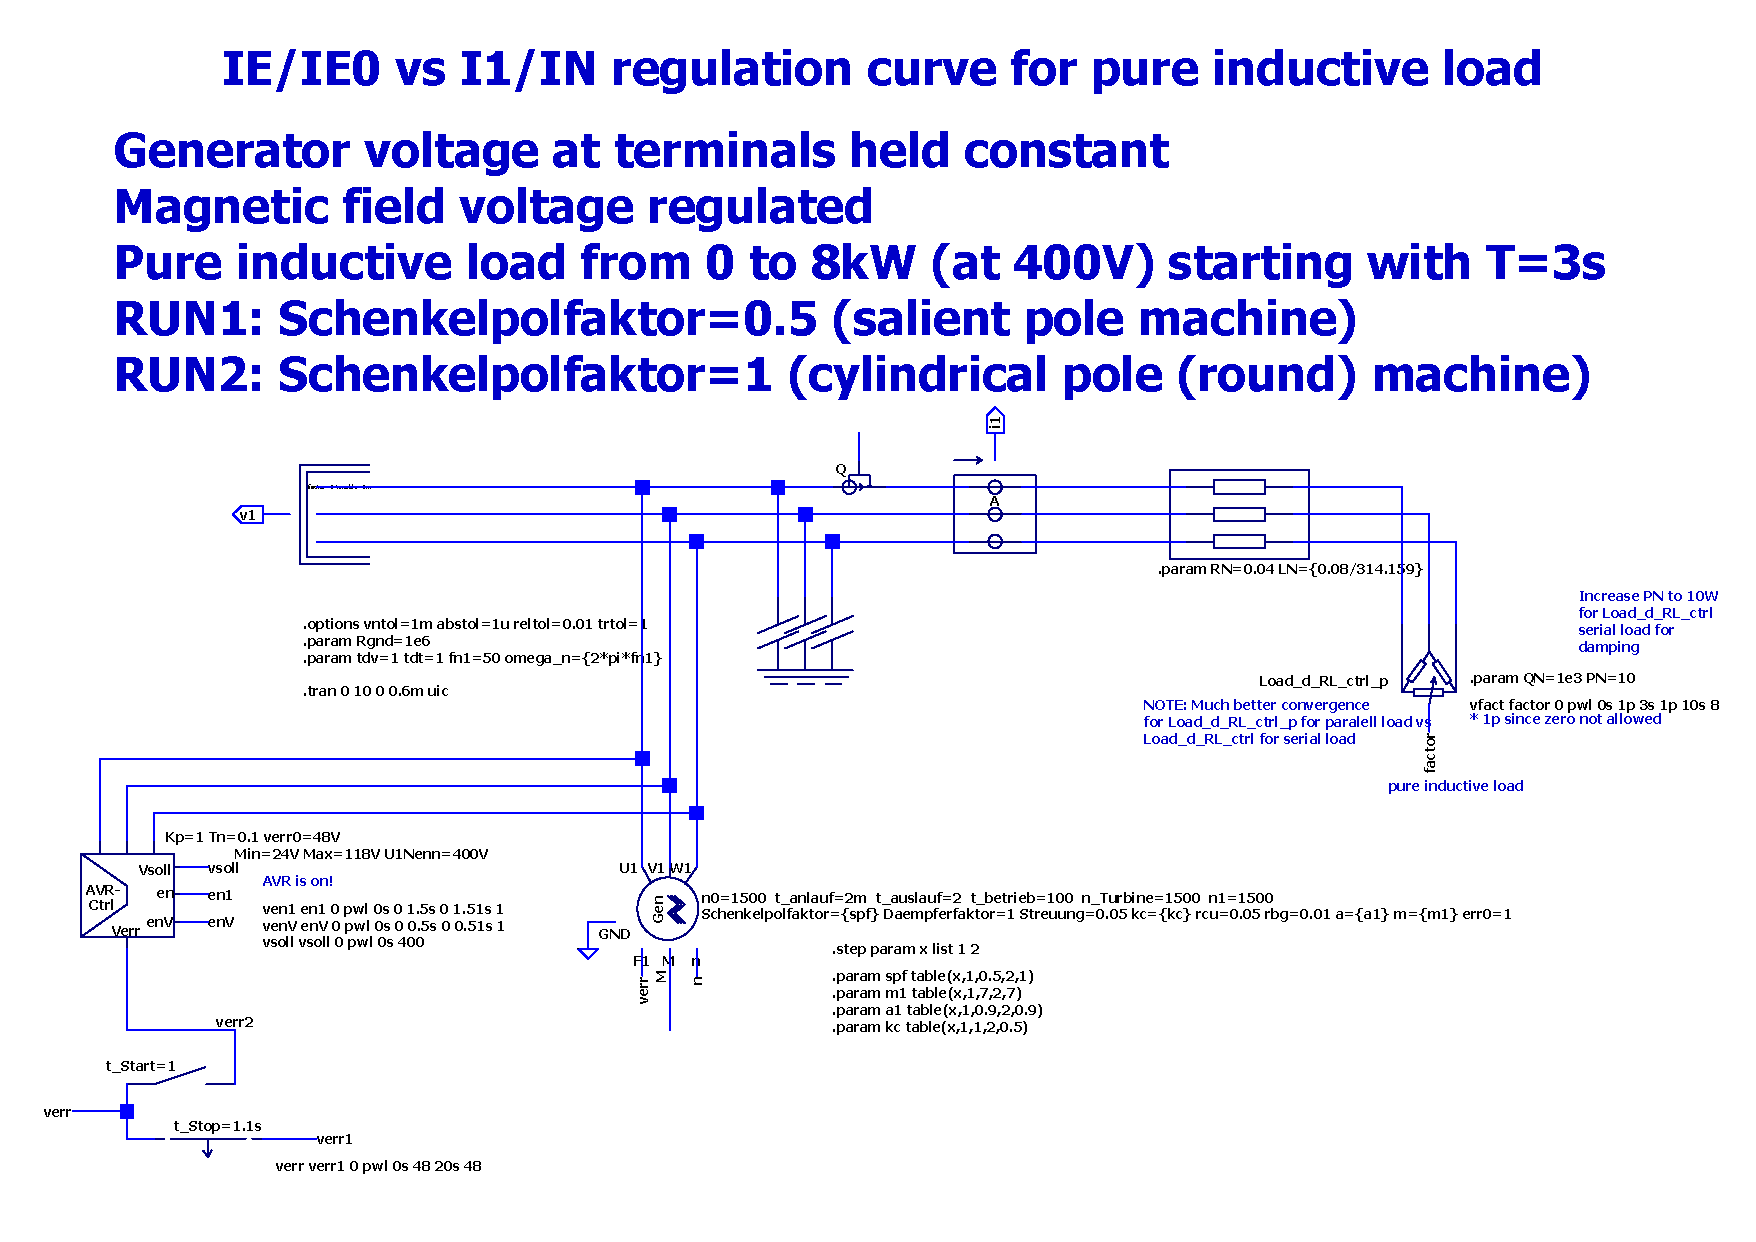
\includegraphics[width=0.9\textwidth] {figures/09_Synchronous_Generator_Characteristic_Curves_400V/sgen_400V_Regulationcurve_inductive_schematic.pdf}
	\caption{Inductive Regulation curve - Schematic}
	\label{fig:figure911}
\end{figure}

\begin{figure}[H]
	\centering
	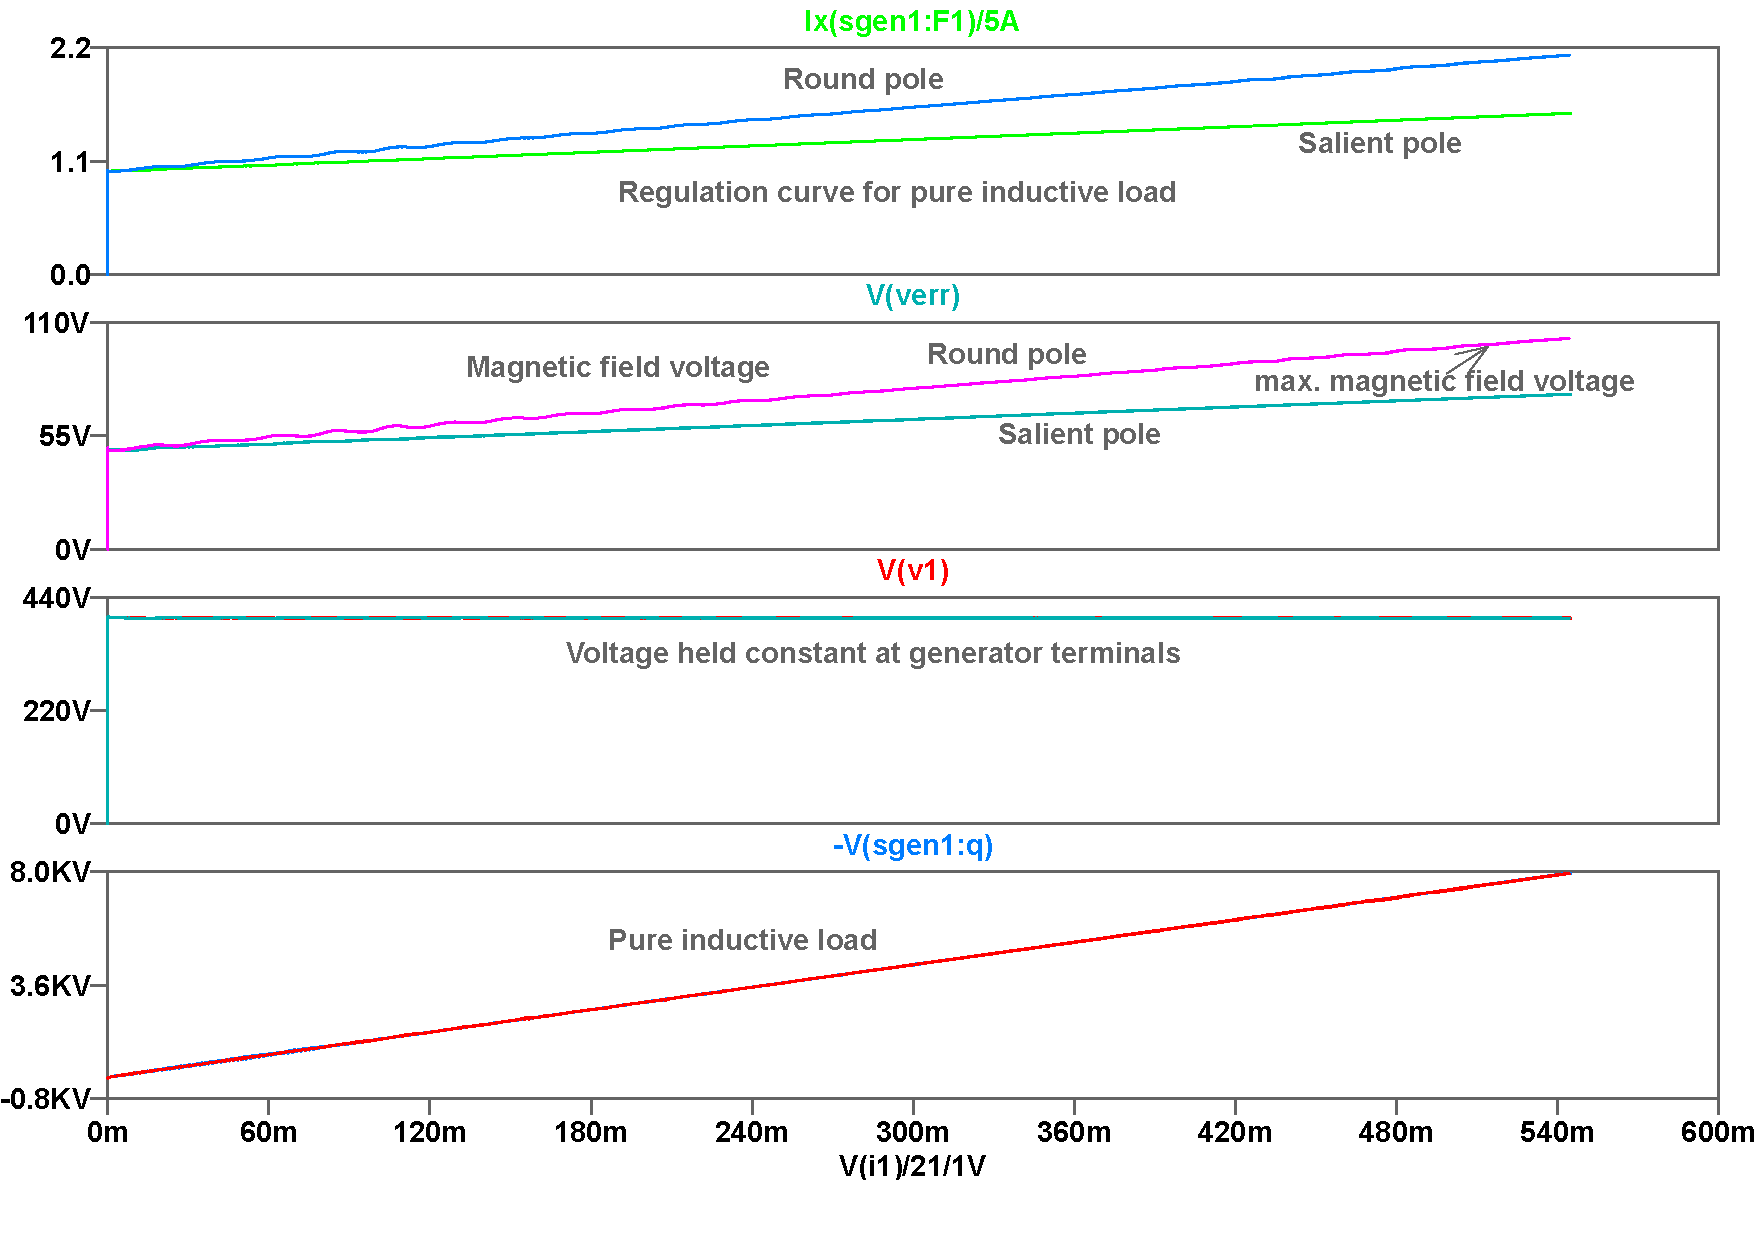
\includegraphics[width=0.9\textwidth] {figures/09_Synchronous_Generator_Characteristic_Curves_400V/sgen_400V_Regulationcurve_inductive_waveform.pdf}
	\caption{Inductive Regulation curve - Waveform}
	\label{fig:figure912}
\end{figure}

\begin{figure}[H]
	\centering
	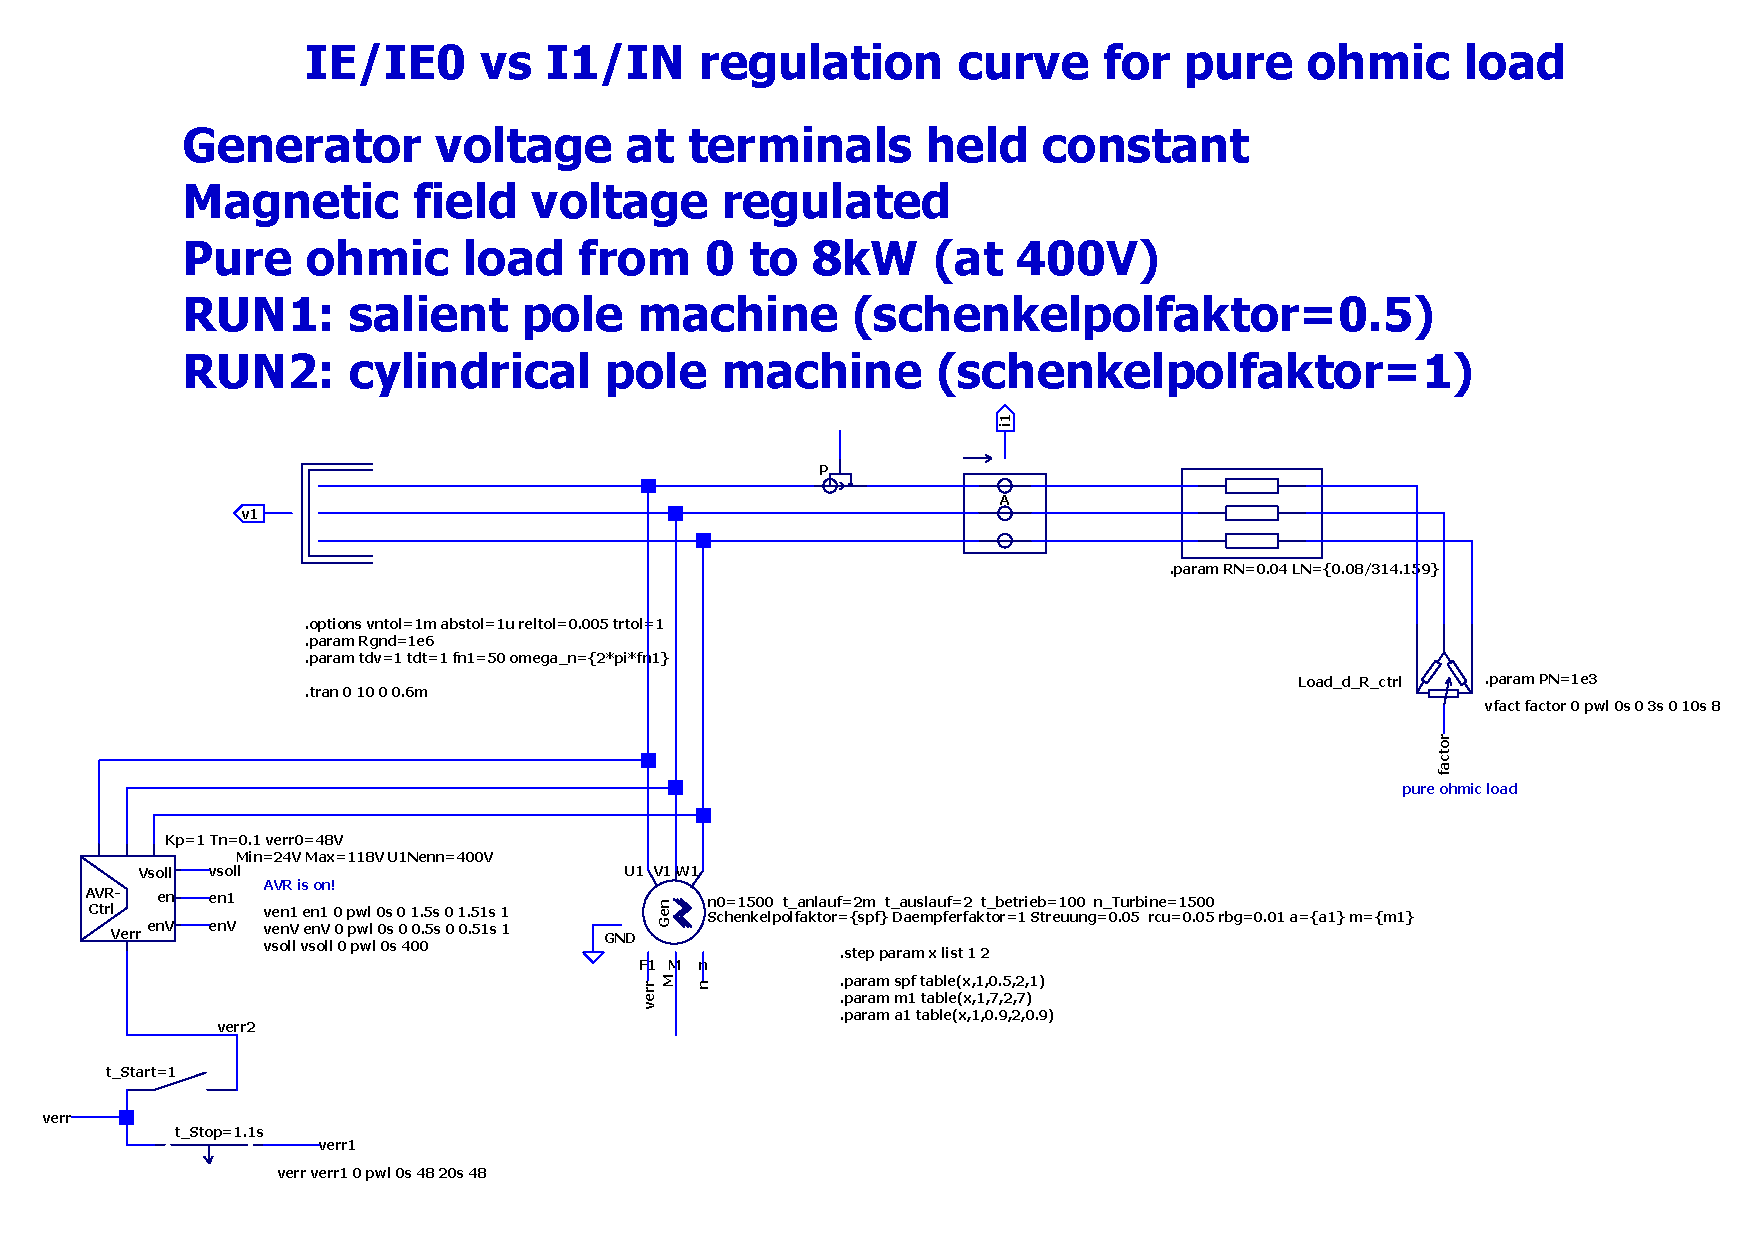
\includegraphics[width=0.9\textwidth] {figures/09_Synchronous_Generator_Characteristic_Curves_400V/sgen_400V_Regulationcurve_ohmic_schematic.pdf}
	\caption{Ohmic  Regulation curve - Schematic}
	\label{fig:figure913}
\end{figure}

\begin{figure}[H]
	\centering
	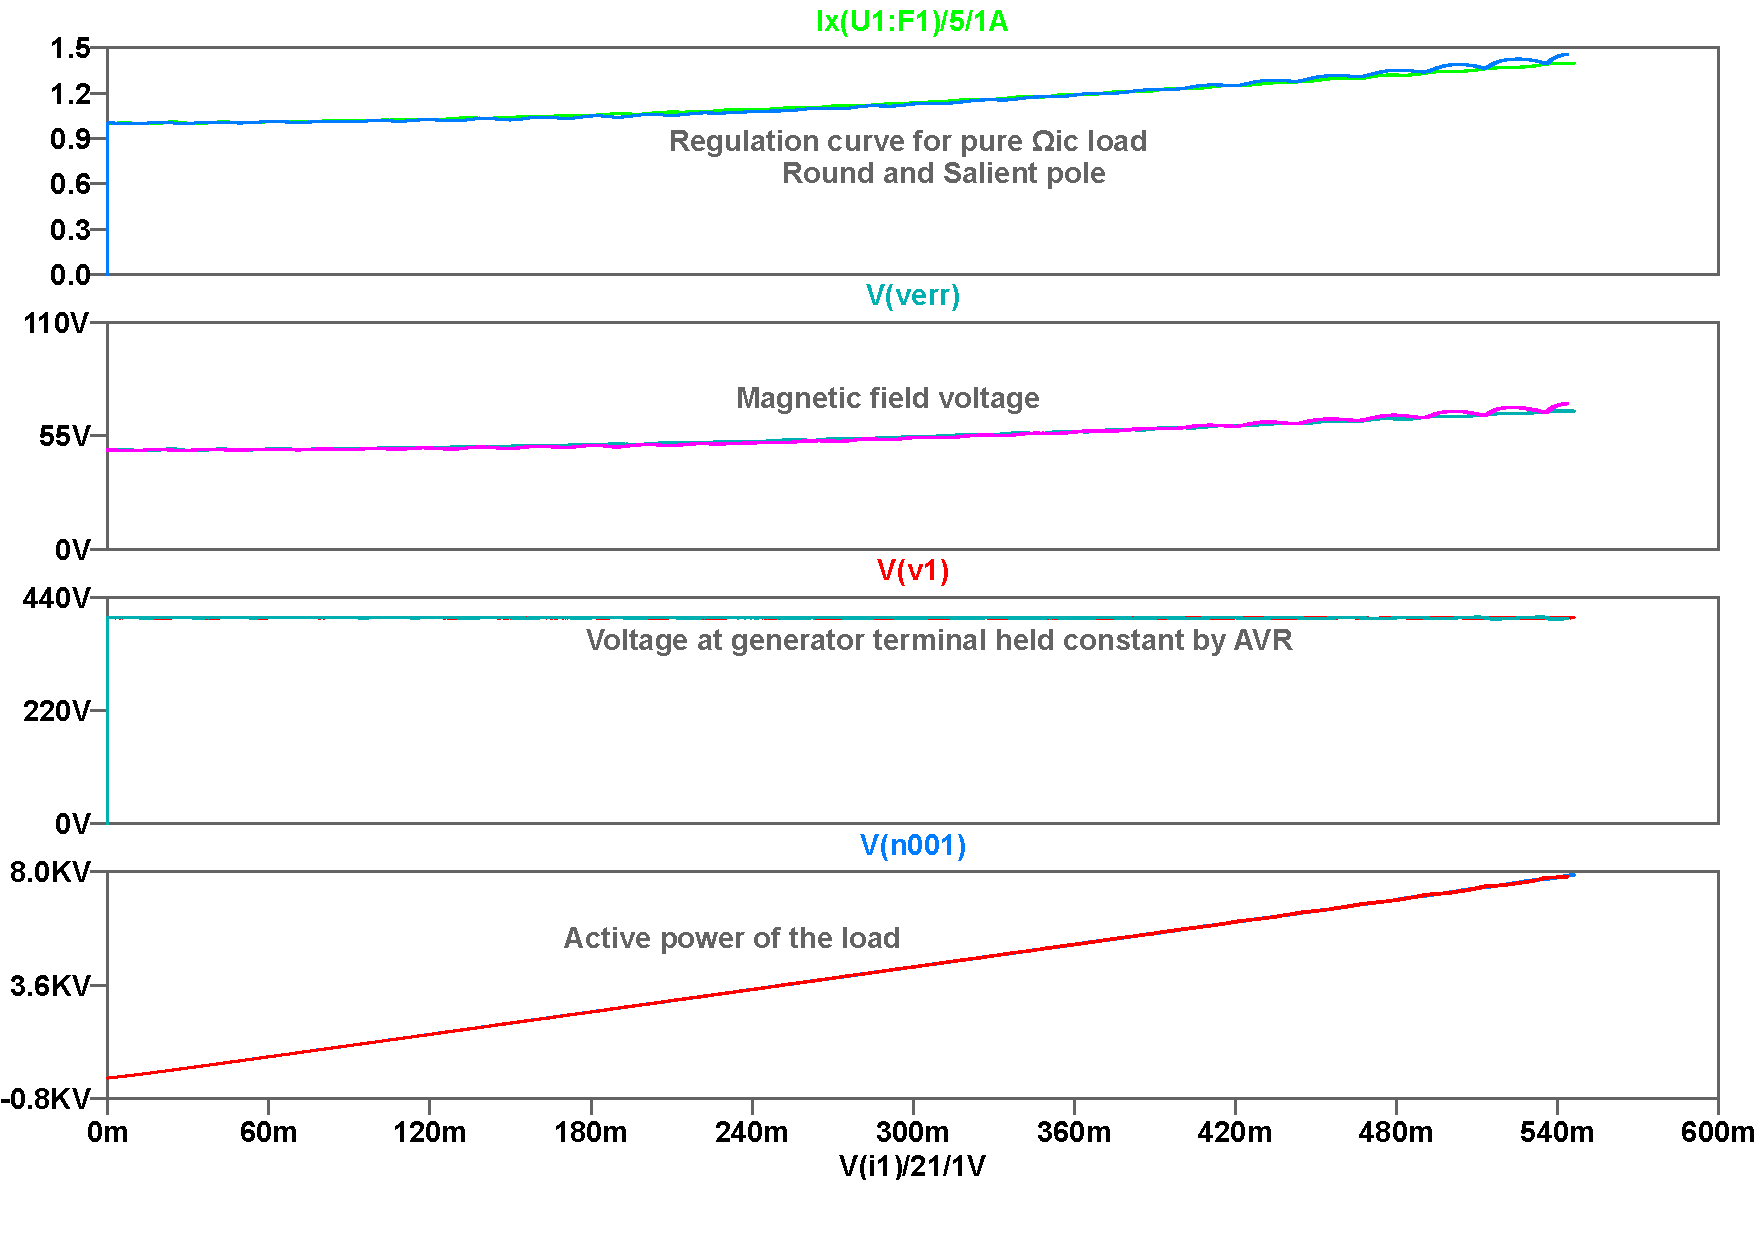
\includegraphics[width=0.9\textwidth] {figures/09_Synchronous_Generator_Characteristic_Curves_400V/sgen_400V_Regulationcurve_ohmic_waveform.pdf}
	\caption{Ohmic  Regulation curve - Waveform}
	\label{fig:figure914}
\end{figure}

\begin{figure}[H]
	\centering
	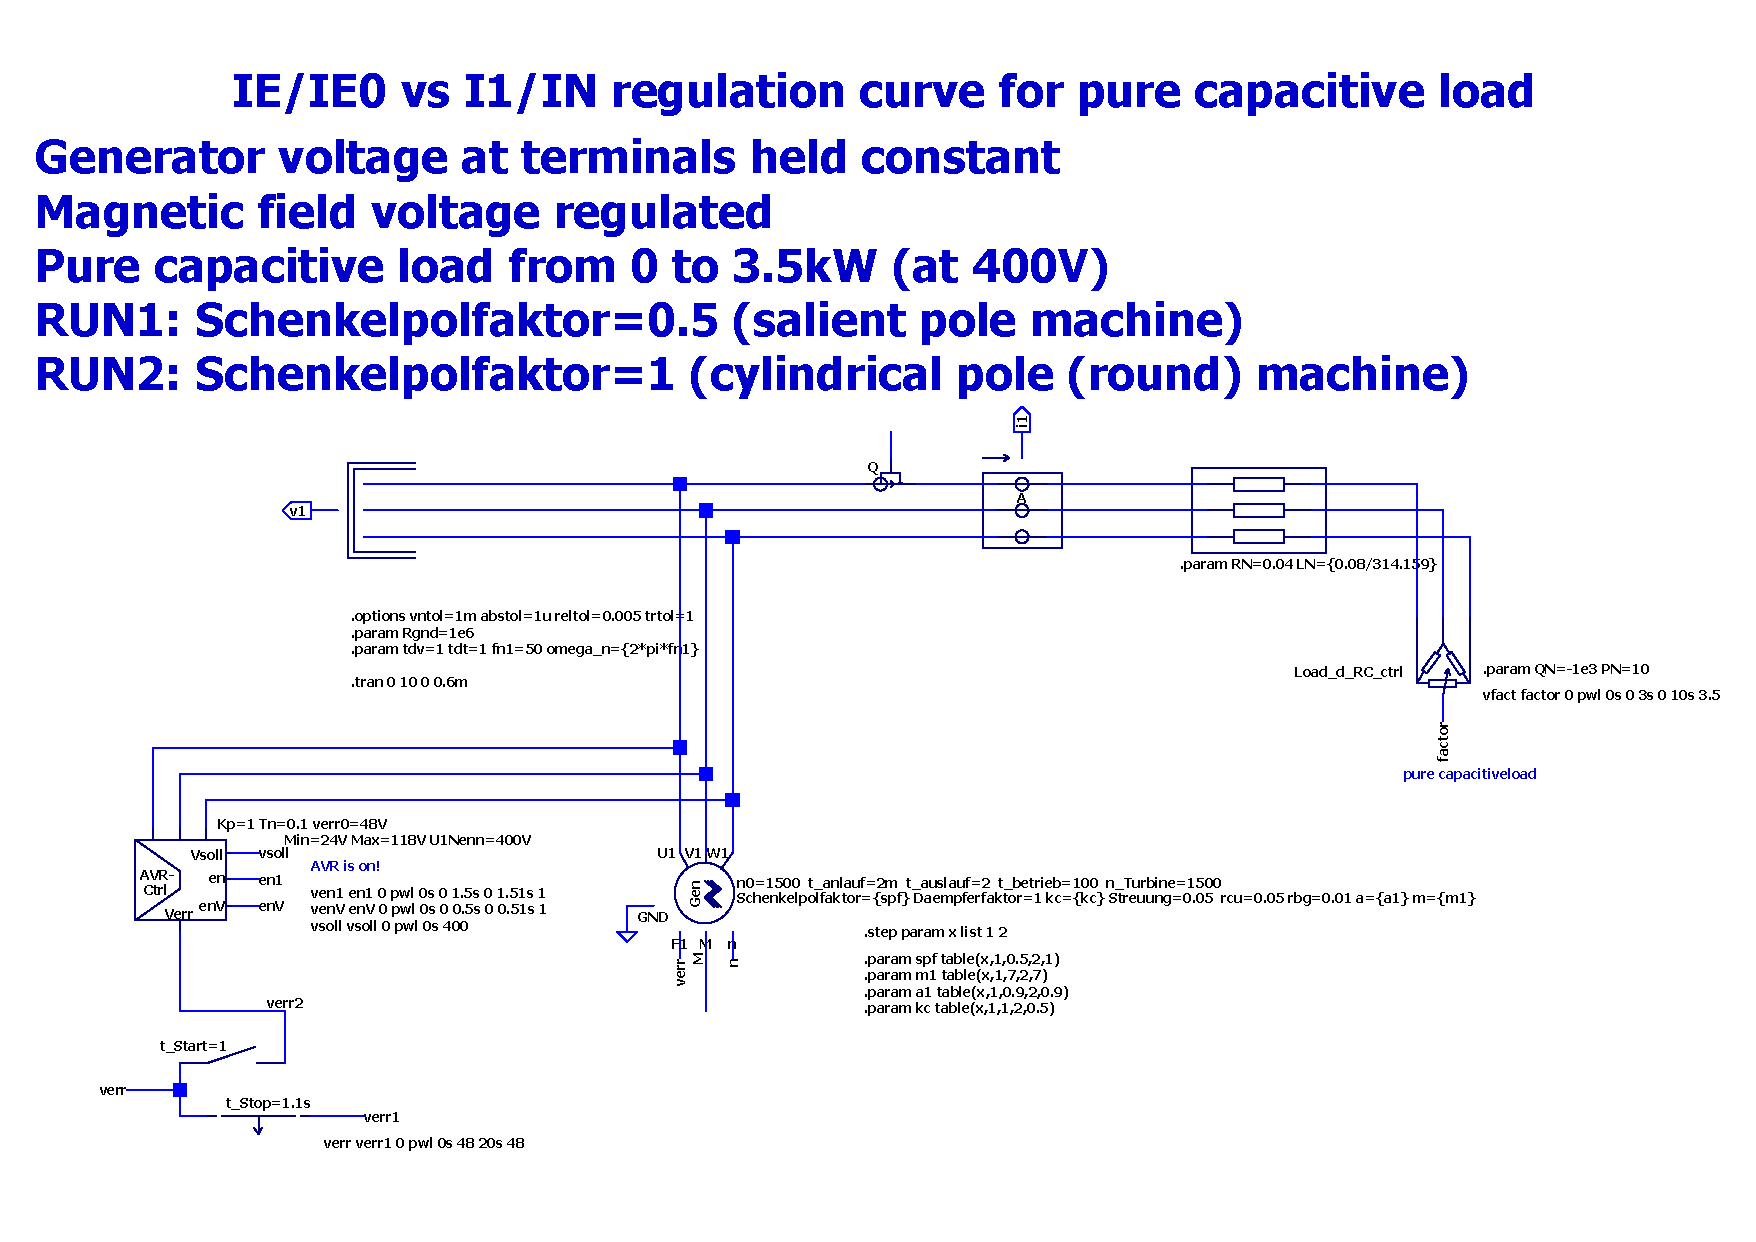
\includegraphics[width=0.9\textwidth] {figures/09_Synchronous_Generator_Characteristic_Curves_400V/sgen_400V_Regulationcurve_capacitive_schematic.pdf}
	\caption{Capacitive  Regulation curve - Schematic}
	\label{fig:figure915}
\end{figure}

\begin{figure}[H]
	\centering
	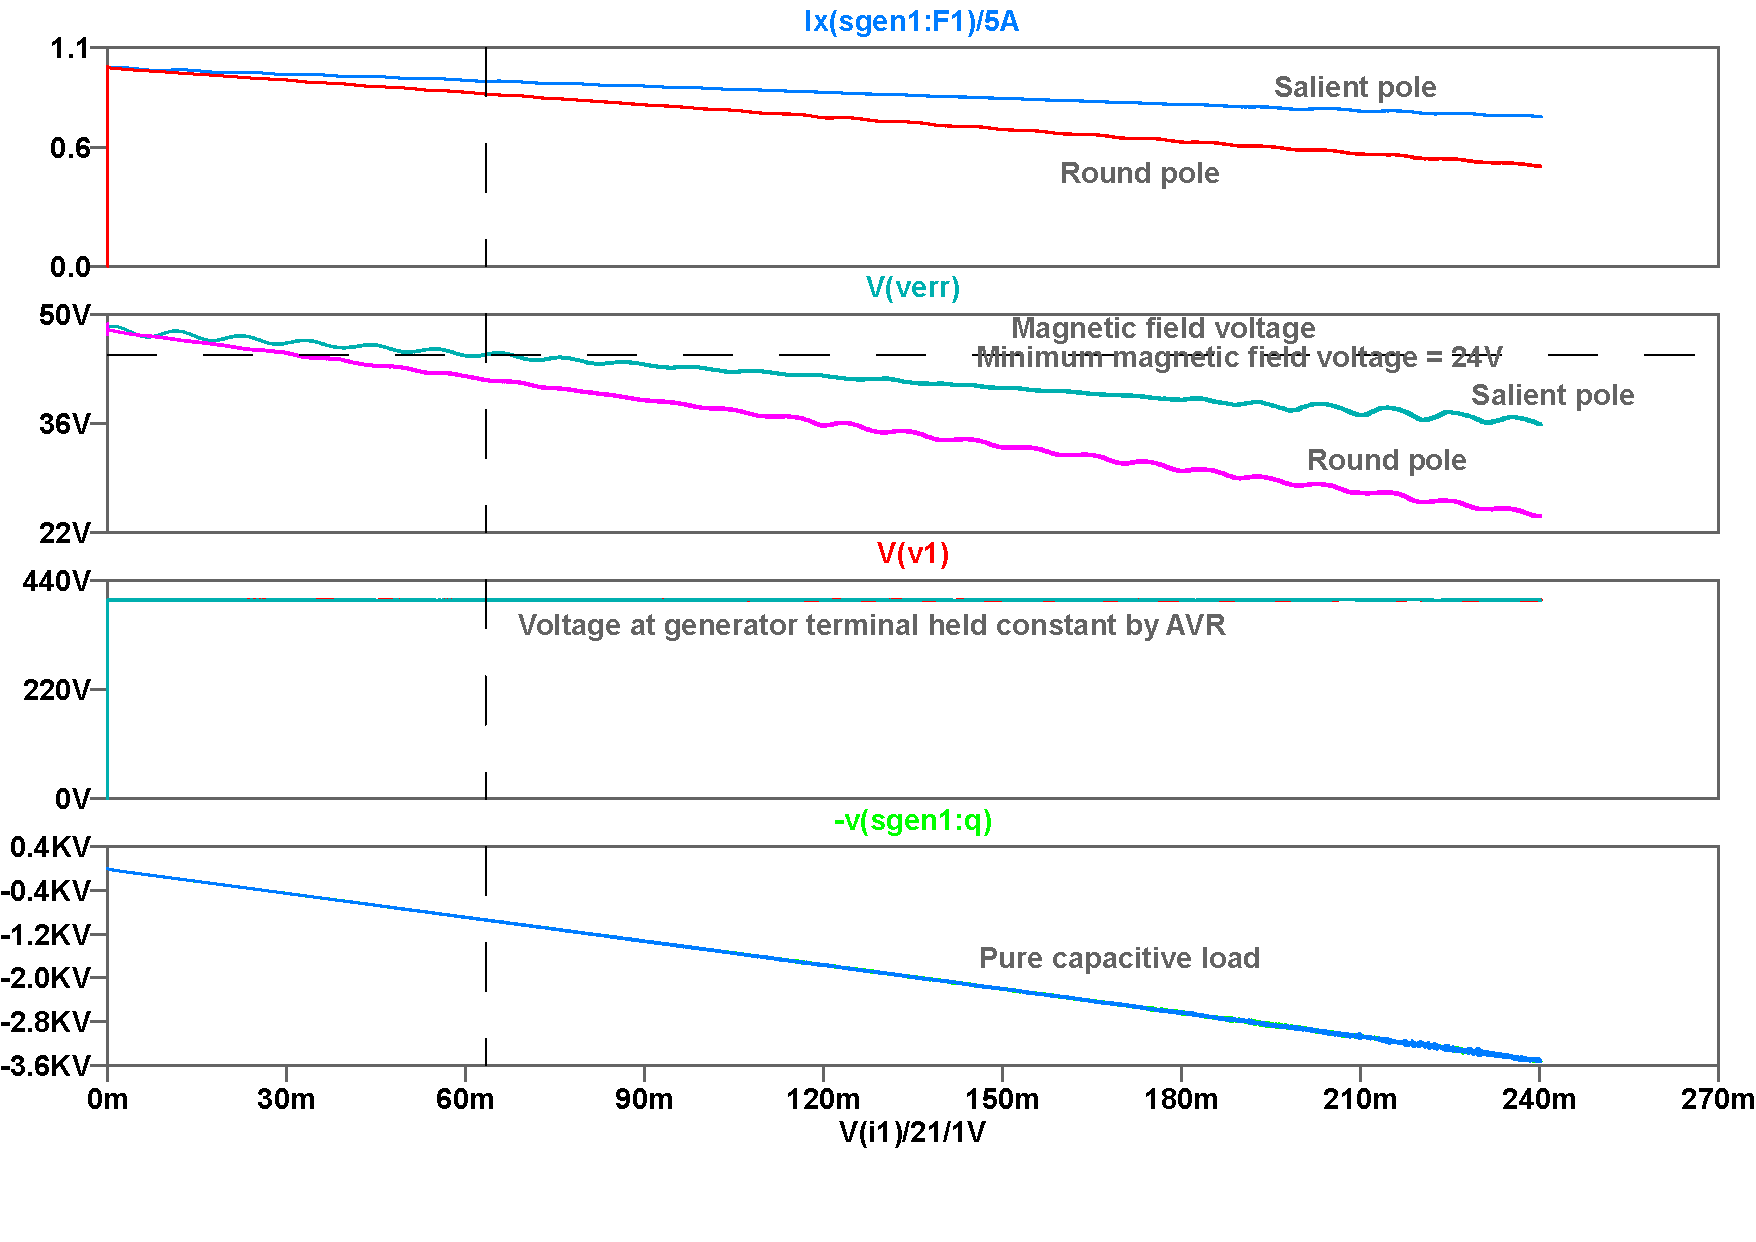
\includegraphics[width=0.9\textwidth] {figures/09_Synchronous_Generator_Characteristic_Curves_400V/sgen_400V_Regulationcurve_capacitive_waveform.pdf}
	\caption{Capacitive  Regulation curve - Waveform}
	\label{fig:figure916}
\end{figure}


% ============================================================
\section{V-Curves} see figure \ref{fig:figure917} and figure \ref{fig:figure918}  (simulation-file: same name as the heading) 
\label{sec:sg-v-curves}
% ============================================================

The V-curves of a synchronous machine show the relationship between stator
current and field current at constant active power and terminal voltage:

\begin{equation}
  I_s=f(I_f),
  \qquad
  P=\text{constant},
  \qquad
  U=\text{constant},
  \qquad
  f=\text{constant}.
  \label{eq:sg-v-curve-definition}
\end{equation}

The curves are named after their characteristic V-shaped appearance.

\subsection{Test Procedure}

The generator is connected to a stiff grid, which maintains approximately
constant voltage and frequency. The mechanical torque is adjusted to establish
a specified active-power output. The field current is then varied while the
mechanical power remains constant. For each excitation value, the stator
current, power factor, and reactive power are recorded.

\subsection{Minimum Stator Current}

For a balanced three-phase generator,

\begin{align}
  S &= \sqrt{3}\,U_{\mathrm{LL}}I_s, \\
  P &= \sqrt{3}\,U_{\mathrm{LL}}I_s\cos\varphi.
\end{align}

At constant active power and terminal voltage,

\begin{equation}
  I_s
  =\frac{P}{\sqrt{3}\,U_{\mathrm{LL}}\cos\varphi}.
  \label{eq:sg-v-curve-current}
\end{equation}

The stator current reaches its minimum when

\begin{equation}
  \cos\varphi=1.
\end{equation}

At this operating point, $Q\approx0$, and the generator exchanges almost no
reactive power with the grid.

\subsection{Underexcited Generator}

If the field current is reduced below the value corresponding to the minimum
stator current, the generator becomes underexcited. Under the usual generator
sign convention, it absorbs reactive power from the grid.

The stator current increases because it contains both an active-current and a
reactive-current component:

\begin{equation}
  I_s=\sqrt{I_P^2+I_Q^2}.
\end{equation}

Although the active power remains constant, the increasing reactive-current
component increases the total stator current. Excessive underexcitation can be
limited by stator heating, end-region heating, reduced steady-state stability,
and the risk of losing synchronism.

\subsection{Overexcited Generator}

If the field current is increased above the value corresponding to unity power
factor, the generator becomes overexcited and normally supplies reactive power
to the grid. The stator current again rises because the magnitude of the
reactive-current component increases.

Excessive overexcitation is limited mainly by rotor field-winding heating,
stator-current heating, magnetic saturation, and the maximum capability of the
excitation system.

\begin{remark}{Reactive-power sign convention}{rem:sg-q-sign}
The statements ``supplies reactive power'' and ``absorbs reactive power'' use
the generator convention. Some simulation programs define positive power as
power entering a component. In that convention, the displayed sign of $Q$ is
reversed and must be checked against the model reference directions.
\end{remark}

\subsection{Families of V-Curves}

A separate V-curve can be recorded for every active-power level, for example,

\begin{equation}
  P=0,
  \quad 0.25P_N,
  \quad 0.5P_N,
  \quad 0.75P_N,
  \quad P_N.
\end{equation}

As active power increases, the minimum possible stator current also increases:

\begin{equation}
  I_{s,\min}
  =\frac{P}{\sqrt{3}\,U_{\mathrm{LL}}}.
\end{equation}

The position of the minimum can shift slightly because of magnetic saturation,
stator resistance, and the synchronous-reactance voltage drop.

\subsection{Inverted V-Curves}

An inverted V-curve represents power factor as a function of field current:

\begin{equation}
  \cos\varphi=f(I_f).
\end{equation}

Its maximum occurs near unity power factor. On one side lies underexcited
operation; on the other lies overexcited operation. Moving away from the
maximum in either direction reduces the magnitude of the power factor and
increases stator current for the same active power.

\subsection{Relationship to Power Control}

The V-curves illustrate the approximate separation of active- and
reactive-power control when a synchronous generator is connected to a stiff
grid:

\begin{itemize}
  \item mechanical torque primarily controls active power $P$,
  \item field excitation primarily controls reactive power $Q$,
  \item the grid frequency fixes the average rotor speed, and
  \item the grid voltage largely fixes the terminal voltage.
\end{itemize}

This separation is not exact because excitation changes also influence the
load angle, saturation, stator current, and machine losses.

\begin{figure}[H]
	\centering
	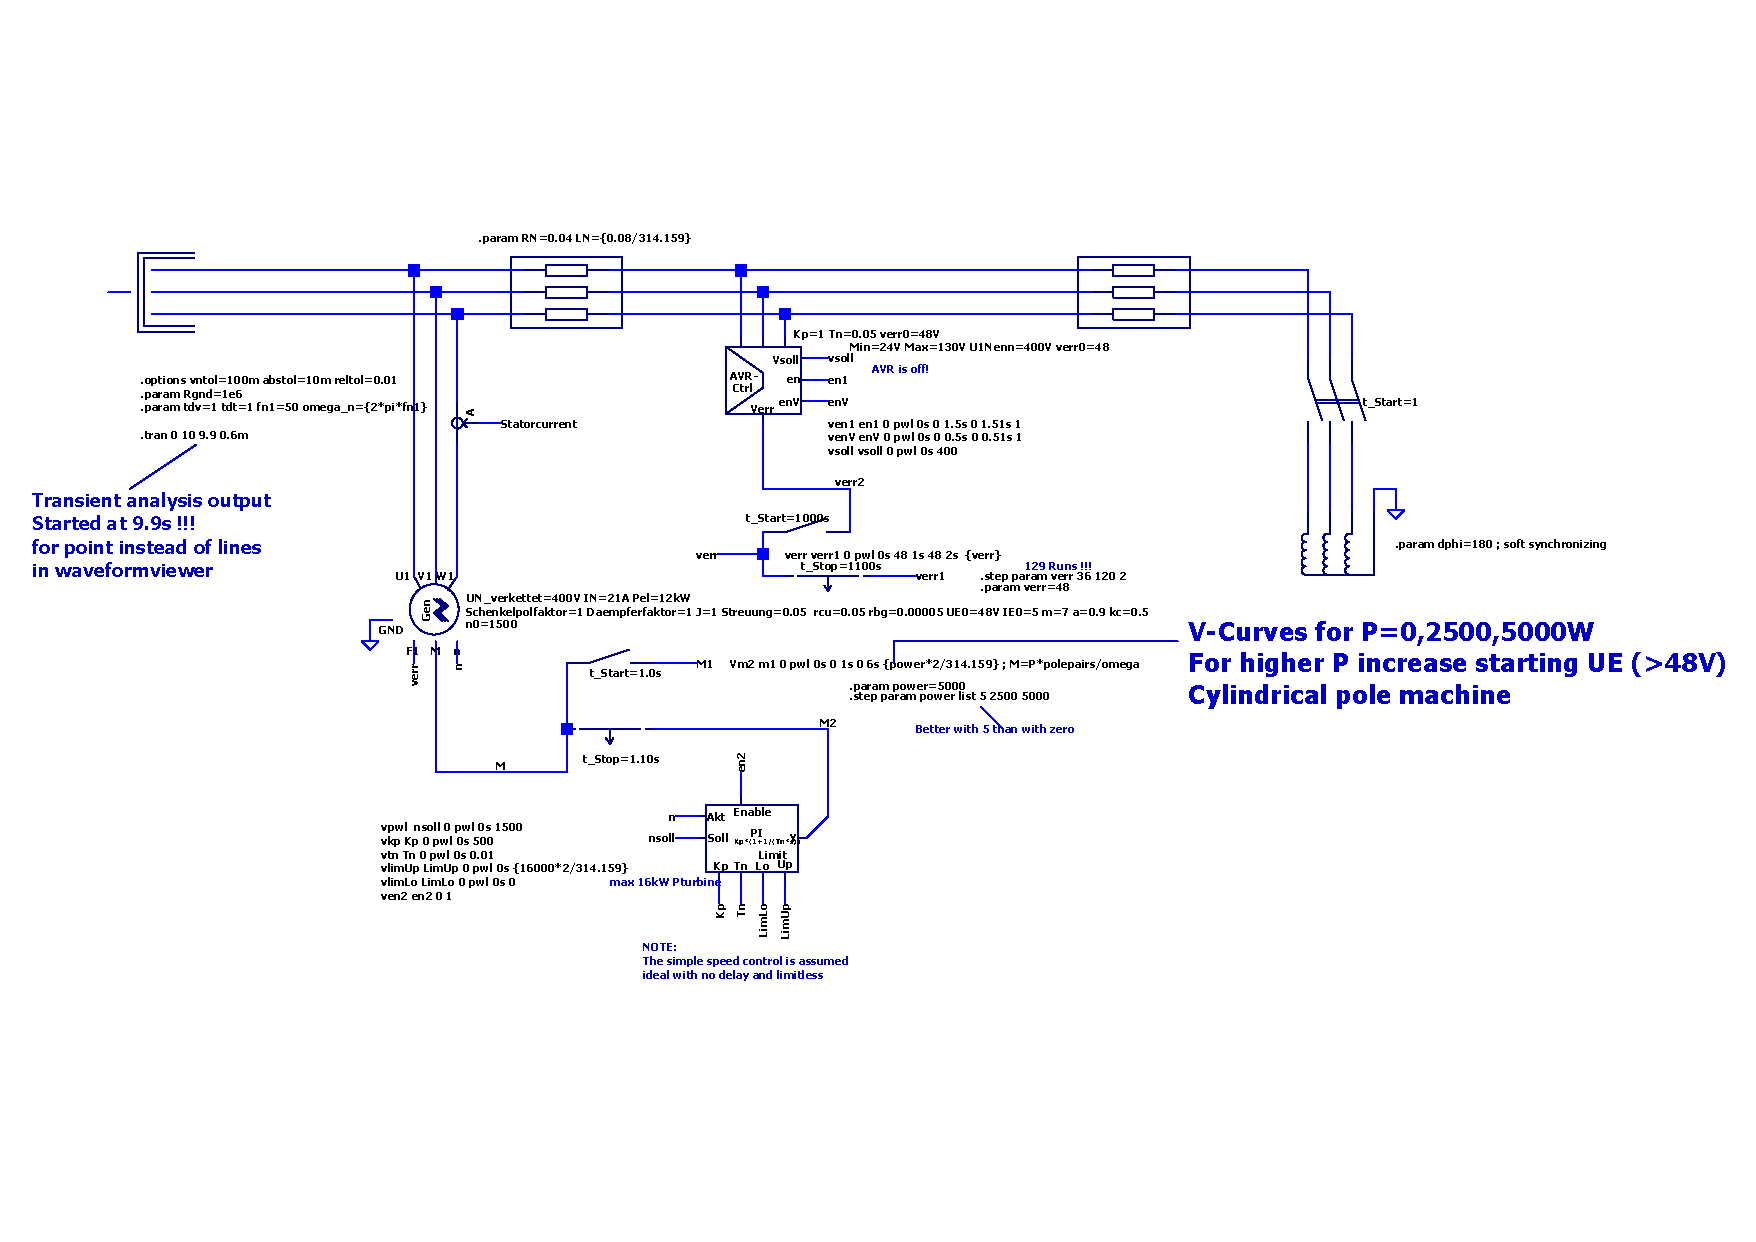
\includegraphics[width=0.9\textwidth] {figures/09_Synchronous_Generator_Characteristic_Curves_400V/sgen_400V_V_curves_multi_schematic.pdf}
	\caption{V-curve - Schematic}
	\label{fig:figure917}
\end{figure}

\begin{figure}[H]
	\centering
	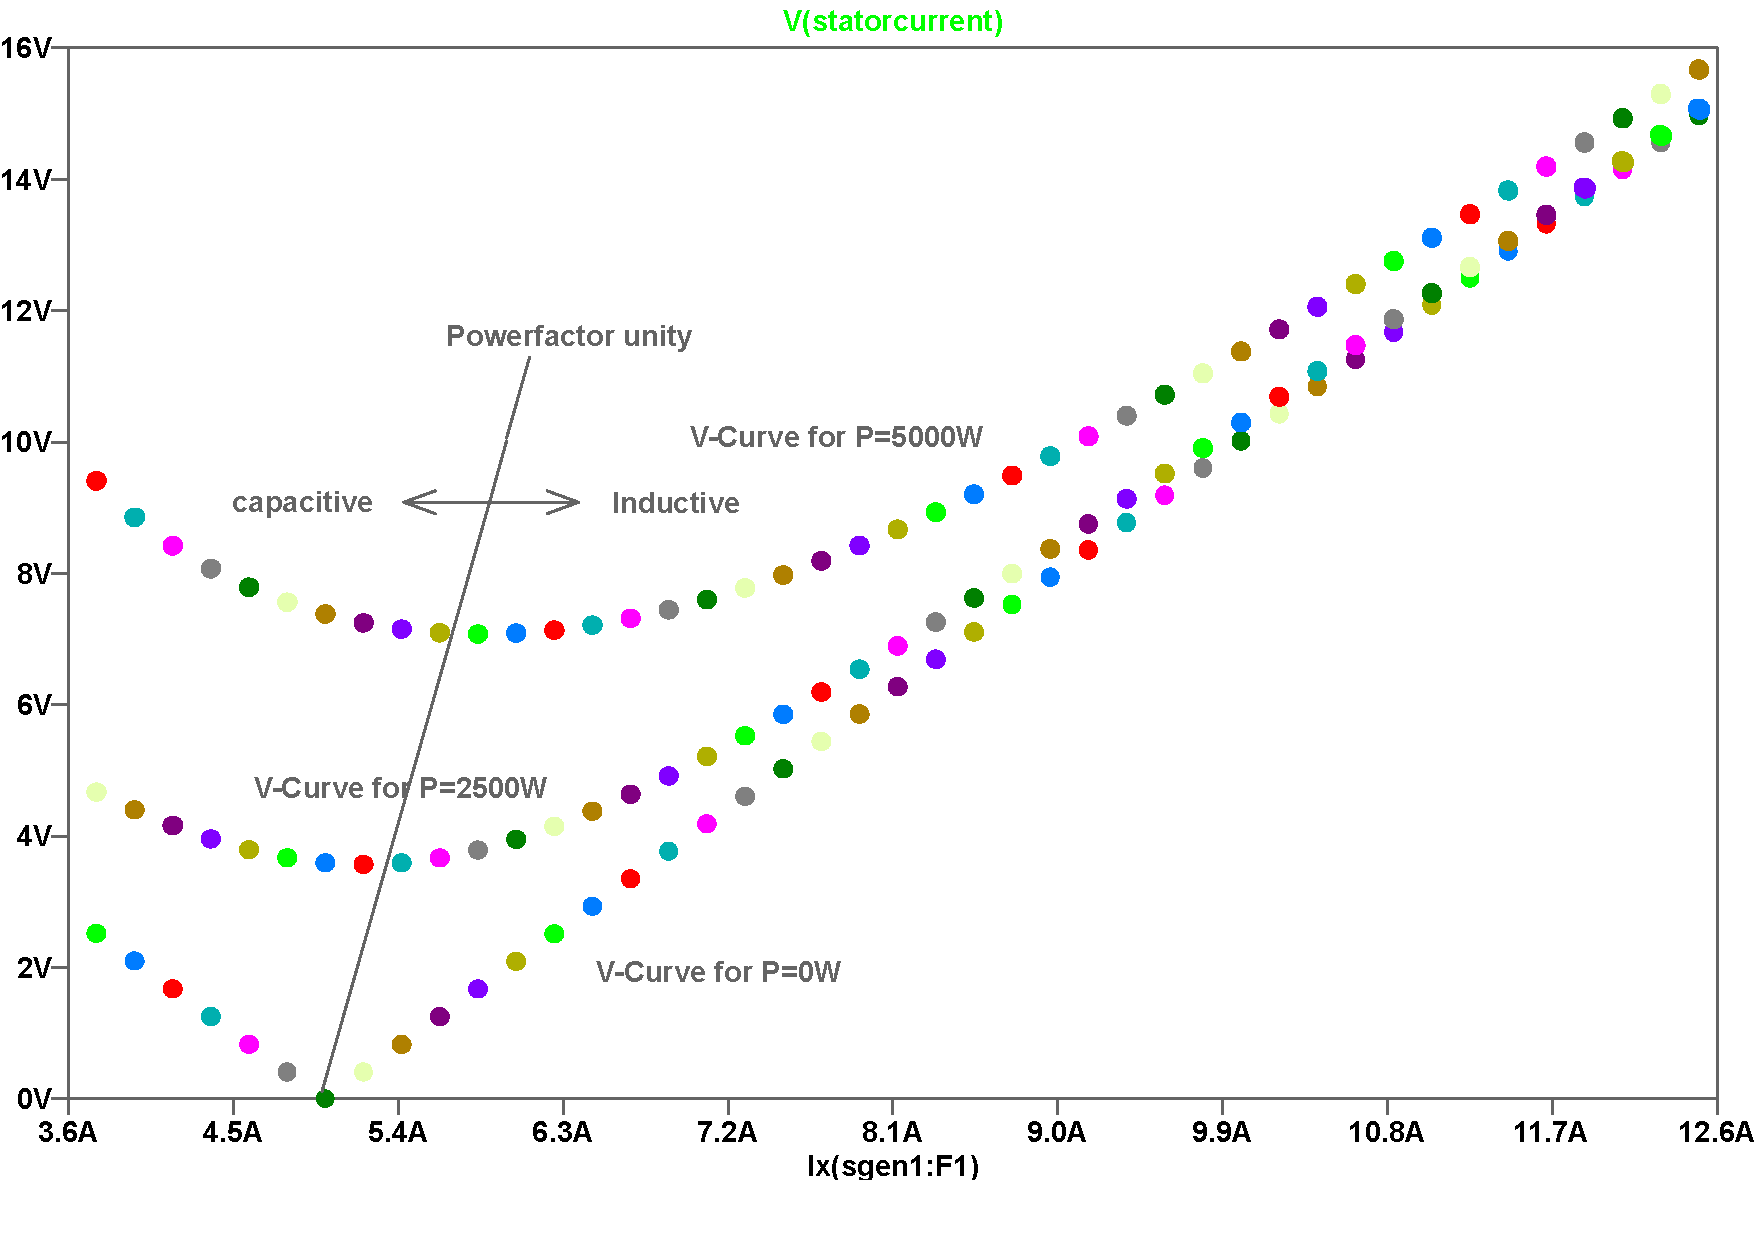
\includegraphics[width=0.9\textwidth] {figures/09_Synchronous_Generator_Characteristic_Curves_400V/sgen_400V_V_curves_multi_waveform.pdf}
	\caption{V-curve - Waveform}
	\label{fig:figure918}
\end{figure}

% ============================================================
\section{Comparison of the Characteristics}
\label{sec:sg-characteristic-comparison}
% ============================================================

\begin{table}[htbp]
  \centering
  \caption{Comparison of synchronous-generator characteristic curves}
  \label{tab:sg-characteristic-curves}
  \small
  \renewcommand{\arraystretch}{1.18}
  \begin{tabularx}{\textwidth}{@{}l c c Y Y@{}}
    \toprule
    \textbf{Characteristic} &
    \textbf{Horizontal axis} &
    \textbf{Vertical axis} &
    \textbf{Constant quantities} &
    \textbf{Main information} \\
    \midrule
    Open circuit & $I_f$ & $U_0$ & $I_s=0$, $n=n_N$ &
      Saturation and generated voltage \\
    Short circuit & $I_f$ & $I_k$ & $U=0$, $n=n_N$ &
      Steady-state fault current and synchronous impedance \\
    Load/external & $I_s$ & $U$ & $I_f$, $n$, $\cos\varphi$ &
      Natural terminal-voltage variation \\
    Regulation & $I_s$ & $I_f$ & $U$, $n$, $\cos\varphi$ &
      Excitation required for constant voltage \\
    V-curve & $I_f$ & $I_s$ & $P$, $U$, $f$ &
      Reactive-power and power-factor behaviour \\
    \bottomrule
  \end{tabularx}
\end{table}

The open-circuit and short-circuit characteristics are principally machine
test characteristics. Together, they provide information about saturation,
synchronous impedance, voltage regulation, and short-circuit ratio.

The load and regulation characteristics describe complementary operating
conditions. The load characteristic shows what happens when excitation remains
unchanged, whereas the regulation characteristic shows how excitation must be
adjusted to prevent the terminal voltage from changing.

The V-curves are mainly operating characteristics. They show the relationship
between excitation, stator current, power factor, and reactive power during
grid-connected operation.

\begin{chaptersummary}
The open-circuit characteristic describes generated voltage and magnetic
saturation. The short-circuit characteristic describes the steady-state fault
current and, together with the OCC, permits an approximate determination of
synchronous impedance and short-circuit ratio.

The load characteristic gives the terminal-voltage variation at constant
excitation, whereas the regulation characteristic gives the field current
required to keep voltage constant. V-curves show how underexcitation and
overexcitation increase stator current and determine whether a grid-connected
generator absorbs or supplies reactive power.
\end{chaptersummary}

% Add further chapters here:
% \include{chapters/02_Transmission_Lines}

% ============================================================
% Appendices
% ============================================================
\appendix

\formulasheettitle{Synchronous Generator Model}%
{Formula sheet for the $xy0$ machine model}
\begin{noteBox}
	\textbf{Notation.} Subscripts $S$, $E$, $DX$, and $DY$ denote the stator,
	excitation winding, and the damper windings on the $x$- and $y$-axes.
	The dot denotes a time derivative, e.g. $\dot\psi=\diff\psi/\diff t$.
	The symbols $x$ and $y$ correspond to the rotating machine axes used in the
	source model.
\end{noteBox}

\begin{formulaBox}{Clarke transformation: three-phase to $xy0$}
	\begin{align}
		u_0   &= \frac{u_1+u_2+u_3}{3}
		= R_0 i_0 + L_0\dot i_0, \\
		u_{SXS} &= \frac{2u_1-(u_2+u_3)}{3}, \\
		u_{SYS} &= \frac{u_2-u_3}{\sqrt{3}}.
	\end{align}
	The stationary components are rotated through the electrical angle $\alpha$:
	\begin{align}
		u_{SX} &= u_{SXS}\cos\alpha + u_{SYS}\sin\alpha, \\
		u_{SY} &= u_{SYS}\cos\alpha - u_{SXS}\sin\alpha.
	\end{align}
\end{formulaBox}

\begin{formulaBox}{Electrical equations in the rotating reference frame}
	\begin{align}
		u_{SX} &= R_S i_{SX}+\dot\psi_{SX}-p\omega\psi_{SY}, \\
		g u_E  &= g^2\frac{2}{3}R_E i_E+\dot\psi_E, \\
		0      &= R_{DX}i_{DX}+\dot\psi_{DX}, \\
		u_{SY} &= R_S i_{SY}+\dot\psi_{SY}+p\omega\psi_{SX}, \\
		0      &= R_{DY}i_{DY}+\dot\psi_{DY}.
	\end{align}
\end{formulaBox}

\newpage
\thispagestyle{scrheadings}

\begin{formulaBox}{Flux linkages and current components}
	The common magnetizing flux linkages are
	\begin{align}
		\psi_{hX}
		&= \psi_{SX}-L_S i_{SX}
		= \psi_{DX}-L_{DX}i_{DX}
		= \psi_E-L_E\frac{i_E}{g}, \\
		\psi_{hY}
		&= \psi_{SY}-L_S i_{SY}
		= \psi_{DY}-L_{DY}i_{DY}.
	\end{align}
	The associated magnetizing currents are
	\begin{align}
		i_{\mu X}=f(\psi_{hX}) &= i_{SX}+i_{DX}+\frac{i_E}{g}, \\
		i_{\mu Y}=f(\psi_{hY}) &= i_{SY}+i_{DY}.
	\end{align}
	
	For the nonlinear magnetization characteristic shown in the source model,
	\begin{equation}
		i_\mu(\psi)=i_{\mu N}
		\left[
		0.9\frac{\psi}{\psi_N}
		+0.1\left(\frac{\psi}{\psi_N}\right)^7
		\right].
	\end{equation}
\end{formulaBox}

\begin{formulaBox}{Mechanical equations}
	\begin{align}
		M &= M_{RBG}-M_i, \\
		M_i &= \frac{3}{2}\,p\left(i_{SY}\psi_{hX}-i_{SX}\psi_{hY}\right), \\
		\alpha &= p\int \omega\,\diff t, \\
		M_{RBG} &= M_{\mathrm{Reibung}}\,\sign(n).
	\end{align}
	Here, $p$ is the number of pole pairs and $n$ is the mechanical speed.
\end{formulaBox}

\begin{formulaBox}{Inverse transformation: $xy0$ to three-phase}
	First rotate from the machine frame back to stationary coordinates:
	\begin{align}
		i_{SXS} &= i_{SX}\cos\alpha-i_{SY}\sin\alpha, \\
		i_{SYS} &= i_{SX}\sin\alpha+i_{SY}\cos\alpha.
	\end{align}
	Then recover the phase currents:
	\begin{align}
		i_1 &= i_{SXS}+i_0, \\
		i_2 &= \frac{-i_{SXS}+\sqrt{3}\,i_{SYS}}{2}+i_0, \\
		i_3 &= \frac{-i_{SXS}-\sqrt{3}\,i_{SYS}}{2}+i_0.
	\end{align}
\end{formulaBox}

\begin{noteBox}
	\textbf{Default model simplifications (if not otherwise supported by the parameter line):}
	\[
	\frac{i_E}{g}=i_E',\qquad
	L_E=L_S,\quad L_0=L_S,\quad L_{DX}=L_S,\quad L_{DY}=L_S,
	\]
	\[
	R_0=R_S,\qquad R_{DX}=R_D,\qquad R_{DY}=R_D.
	\]
\end{noteBox}

%\newpage
\thispagestyle{scrheadings}

\begin{formulaBox}{Constant machine parameters}
	The rated input data used for the \SI{400}{\mega\watt} synchronous generator are
	\begin{align}
		U_{N,\mathrm{verkettet}}&=\SI{20}{\kilo\volt}, &
		I_N&=\SI{14.434}{\kilo\ampere}, &
		P_{EL}&=\SI{400}{\mega\watt},\\
		f_N&=\SI{50}{\hertz}, &
		K_C&=0.5, &
		p&=2,\\
		U_{E0}&=\SI{600}{\volt}, &
		I_{E0}&=\SI{2000}{\ampere}, &
		\mathrm{Streuung}&=0.05,\\
		r_{cu}&=0.001, &
		r_{bg}&=0.001, &
		\mathrm{Schenkelpolfaktor}&=1,\\
		\mathrm{Daempferfaktor}&=1. &&&
	\end{align}
	
	The apparent power and power factor obtained from the rated voltage and current
	are
	\begin{align}
		S_N
		&=\sqrt{3}\,U_{N,\mathrm{verkettet}}I_N\\
		&=\sqrt{3}\cdot\SI{20}{\kilo\volt}
		\cdot\SI{14.434}{\kilo\ampere}
		=\SI{500.008}{\mega\volt\ampere}
		\approx\SI{500}{\mega\volt\ampere},\\
		\cos\varphi_N
		&=\frac{P_{EL}}{S_N}
		=\frac{\SI{400}{\mega\watt}}
		{\SI{500.008}{\mega\volt\ampere}}
		=0.799987\approx0.8.
	\end{align}
	
	The constant machine parameters are calculated from
	\begin{align}
		U_N &= \frac{U_{N,\mathrm{verkettet}}}{\sqrt{3}}, &
		Z_N &= \frac{U_N}{I_N}, \\
		\omega_{EL} &= 2\pi f_N, &
		R_S &= Z_N\,r_{cu}, \\
		L_S &= \frac{\mathrm{Streuung}\,Z_N}{K_C\omega_{EL}}, &
		\Psi_N &= \frac{\sqrt{2}\,U_N}{\omega_{EL}}, \\
		g &= \frac{I_{E0}(1-\mathrm{Streuung})}
		{K_C\sqrt{2}\,I_N}, &
		R_D &= \frac{R_S}{\mathrm{Daempferfaktor}}, \\
		I_{MNX} &= \frac{I_{E0}}{g}, &
		I_{MNY} &= \frac{I_{MNX}}{\mathrm{Schenkelpolfaktor}}, \\
		M_N &= \frac{pP_{EL}(1-r_{bg}-r_{cu})}{\omega_{EL}}. &&
	\end{align}
	
	Inserting the rated data gives
	\begin{align}
		U_N
		&=\frac{\SI{20}{\kilo\volt}}{\sqrt{3}}
		=\boxed{\SI{11.5470}{\kilo\volt}},\\
		Z_N
		&=\frac{\SI{11.5470}{\kilo\volt}}
		{\SI{14.434}{\kilo\ampere}}
		=\boxed{\SI{0.799987}{\ohm}},\\
		\omega_{EL}
		&=2\pi\cdot\SI{50}{\hertz}
		=\boxed{\SI{314.159}{\radian\per\second}},\\
		R_S
		&=\SI{0.799987}{\ohm}\cdot0.001
		=\boxed{\SI{7.99987e-4}{\ohm}},\\
		L_S
		&=\frac{0.05\cdot\SI{0.799987}{\ohm}}
		{0.5\cdot\SI{314.159}{\radian\per\second}}
		=\boxed{\SI{2.54644e-4}{\henry}},\\
		\Psi_N
		&=\frac{\sqrt{2}\cdot\SI{11.5470}{\kilo\volt}}
		{\SI{314.159}{\radian\per\second}}
		=\boxed{\SI{51.9798}{\weber}}.
	\end{align}
	
	For the excitation-current transformation,
	\begin{align}
		g
		&=\frac{\SI{2000}{\ampere}(1-0.05)}
		{0.5\sqrt{2}\cdot\SI{14.434}{\kilo\ampere}}
		=\boxed{0.186158},\\
		I_{MNX}
		&=\frac{\SI{2000}{\ampere}}{0.186158}
		=\boxed{\SI{10.7436}{\kilo\ampere}},\\
		I_{MNY}
		&=\frac{\SI{10.7436}{\kilo\ampere}}{1}
		=\boxed{\SI{10.7436}{\kilo\ampere}}.
	\end{align}
	
	Because \(\mathrm{Daempferfaktor}=1\), the damper resistance becomes
	\begin{equation}
		R_D=\frac{R_S}{1}
		=\boxed{\SI{7.99987e-4}{\ohm}}.
	\end{equation}
	
	The rated electromagnetic torque, including the specified relative friction
	and copper losses, is
	\begin{align}
		M_N
		&=\frac{2\cdot\SI{400}{\mega\watt}
			(1-0.001-0.001)}
		{\SI{314.159}{\radian\per\second}}\\
		&=\boxed{\SI{2.54139e6}{\newton\metre}}.
	\end{align}
	
	The excitation-winding resistance and its resistance referred to the stator side
	equation are
	\begin{align}
		R_E
		&=\frac{U_{E0}}{I_{E0}}
		=\frac{\SI{600}{\volt}}{\SI{2000}{\ampere}}
		=\boxed{\SI{0.300000}{\ohm}},\\
		R_E'
		&=g^2\frac{2}{3}R_E
		=(0.186158)^2\frac{2}{3}\cdot\SI{0.3}{\ohm}
		=\boxed{\SI{6.93097e-3}{\ohm}},\\
		U_{E0}'
		&=gU_{E0}
		=0.186158\cdot\SI{600}{\volt}
		=\boxed{\SI{111.695}{\volt}}.
	\end{align}
	
	For \(p=2\), the synchronous mechanical speed is
	\begin{align}
		n_N&=\frac{60f_N}{p}
		=\boxed{\SI{1500}{\rpm}}, &
		\omega_{mN}&=\frac{\omega_{EL}}{p}
		=\boxed{\SI{157.080}{\radian\per\second}}.
	\end{align}
	
\end{formulaBox}

\begin{noteBox}
	\textbf{Interpretation of \(\Psi_N\).}
	The value \(\Psi_N=\SI{51.9798}{\weber}\) is the rated peak stator flux
	linkage in volt-seconds, not the physical air-gap flux in webers per pole. A
	physical flux value would additionally require the effective number of stator
	turns and the winding factor.
\end{noteBox}

\begin{formulaBox}{Parameter definitions}
	\renewcommand{\arraystretch}{\formulaTableStretch}
	\begin{tabularx}{\textwidth}{>{\bfseries\(}l<{\)} X}
		\toprule
		\text{Symbol} & \textbf{Meaning} \\
		\midrule
		\mathrm{Streuung} & Leakage factor \\
		\mathrm{Daempferfaktor} & Damping factor \\
		\mathrm{Schenkelpolfaktor} & Salient-pole factor \\
		r_{bg} & Friction-loss factor \\
		r_{cu} & Copper-loss (resistance) factor \\
		p & Number of pole pairs \\
		K_C & Model scaling or correction factor \\
		U_{N,\mathrm{verkettet}} & Rated line-to-line RMS voltage \\
		U_N,\ I_N,\ Z_N & Rated phase voltage, rated current, and base impedance \\
		f_N,\ \omega_{EL} & Rated electrical frequency and angular frequency \\
		I_{E0} & Reference excitation current \\
		P_{EL} & Electrical power \\
		\bottomrule
	\end{tabularx}
\end{formulaBox}

\begin{widefigure}{Synchronous machine schematic model}{schematic111}
	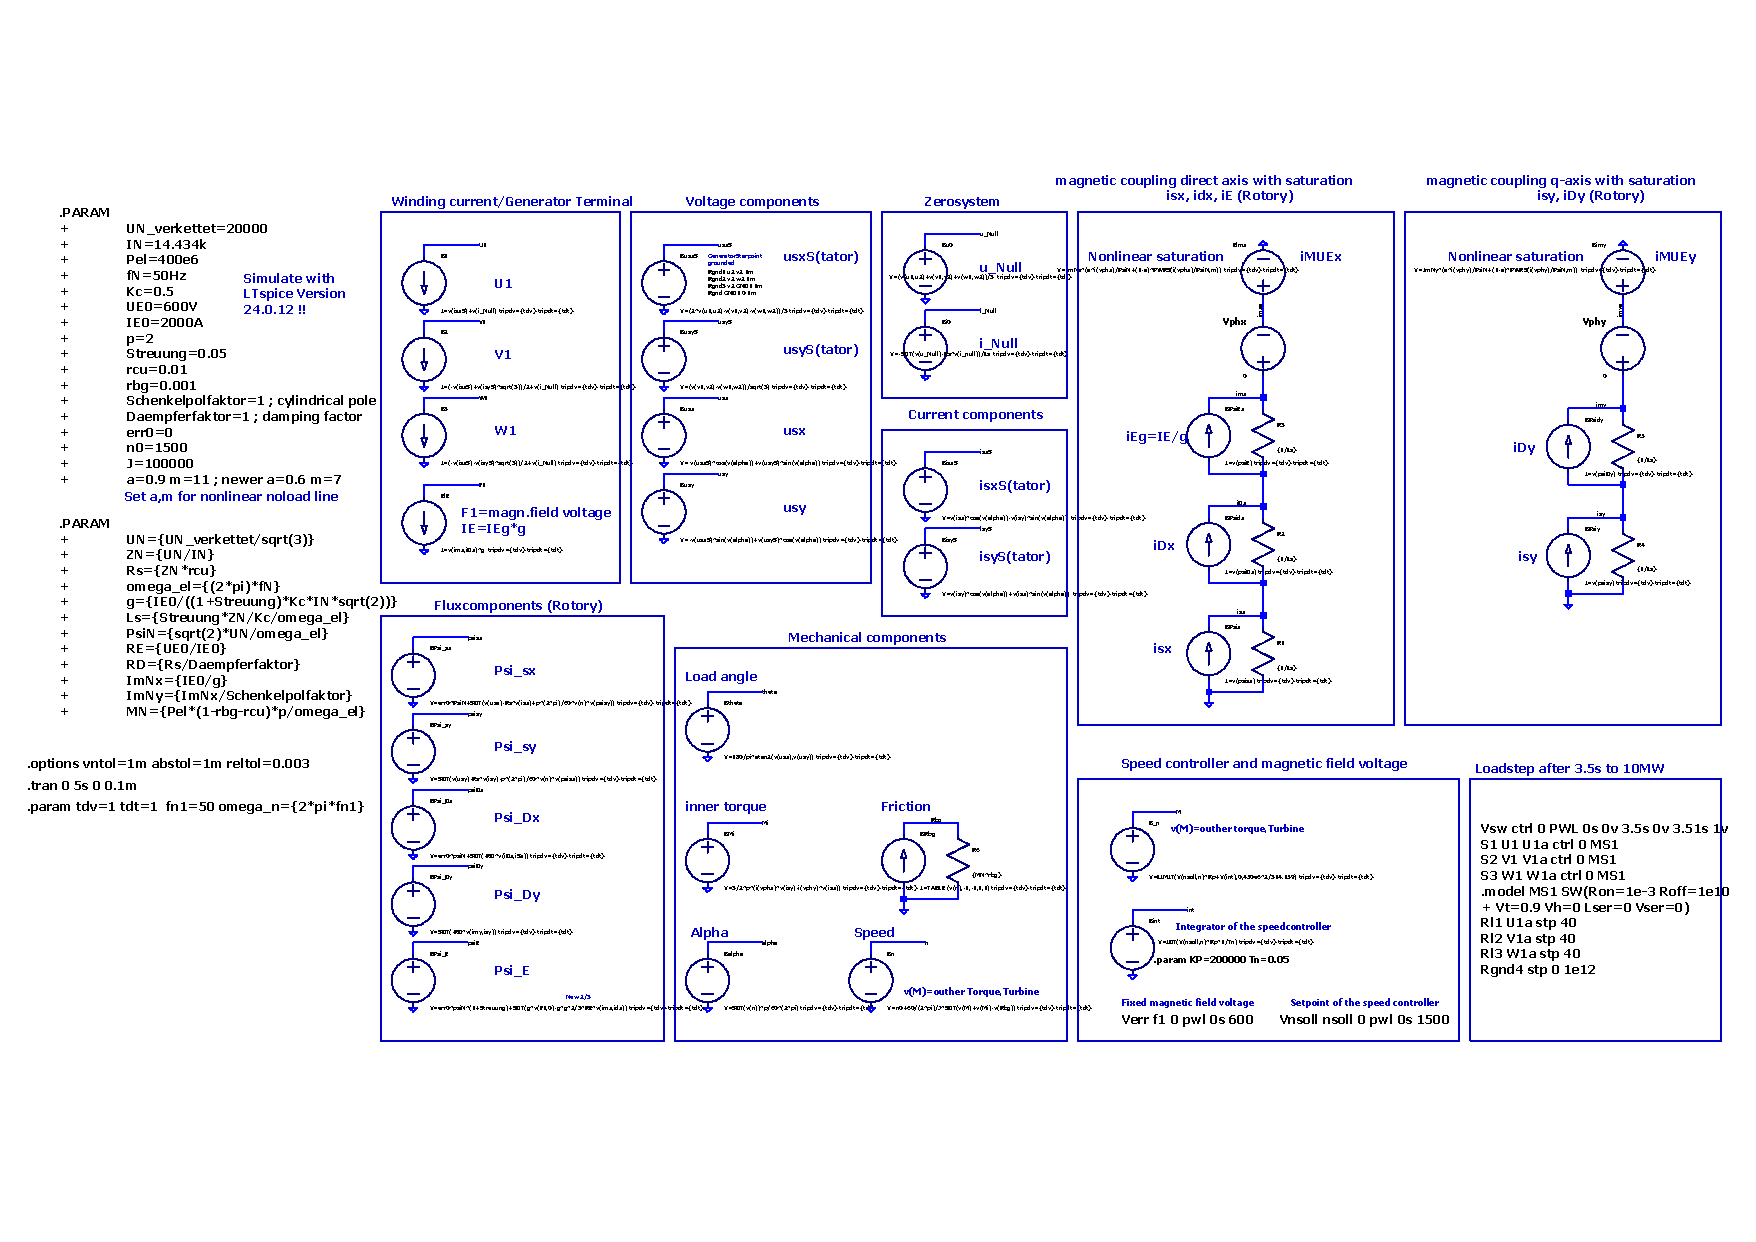
\includegraphics[width=1.5\textwidth]{figures/Synchronous_generator_model.pdf}
\end{widefigure}

%\begin{figure}[H]
%	\centering
%	\includegraphics[width=0.99\textwidth]{figures/Transformer_and_shunt_reactor_AC_Schematic}
%	\caption{Schematic for the Transformer and shunt reactor circuit.}
%	\label{fig:Transformer_and_shunt_reactor_AC_Schematic}
%\end{figure}

\begin{lstlisting}[style=LTspice,caption={Behavioral implementation of a synchronous generator.},label={lst:synchronous generator}]
1 * NOTE: idt() = integration function
2 .SUBCKT Block1_fixe_Drehzahl U1 V1 W1 F1 M n GND1
3 + PARAMS:
4 + UN_verkettet=20000
5 + IN=14.434k
6 + Pel=400e6 ;UN_verkettet*IN*sqrt(3)*cosphi of 0.8
7 + fn=50
8 + Kc=0.5
9 + UE0=600V ; Power of exciter = 0.25-5% * SN machine (smaller values for higher SN)
10 + IE0=2000A
11 + p=2
12 + Streuung=0.05 ;
13 + rcu=0.001
14 + rbg=0.001
15 + Schenkelpolfaktor=1 ;(1=cylindrical pole 0.5=Salient pole)
16 + Daempferfaktor=1
17 + err0=0
18 + RE_factor=0.6666
19 + n0=1500
20 + n1={n0} ;starts with 1500U/min
21 + alpha_0=0
22 + a=0.9 ; Parameter for nonlinear noload line (should be about 0.6-0.9)
23 + m=7
24 .PARAM
25 + a1={a}; Saturation parameter d-axis
26 + m1={m}; Saturation parameter d-axis
27 + a2={a1}; Saturation parameter q-axis
28 + m2={m1}; Saturation parameter q-axis
29 + UN={UN_verkettet/sqrt(3)}
30 + ZN={UN/IN}
31 + Rs={ZN*rcu}
32 + omega_el={(2*pi)*fN}
33 + Ls={Streuung*ZN/Kc/omega_el}
34 + PsiN={sqrt(2)*UN/omega_el}
35 + RE={UE0/IE0}
36 + RD={Rs/Daempferfaktor}
37 + RDx={RD} ; can be overwritten by setting this parameters on modelline
38 + RDy={RD} ; can be overwritten by setting this parameters on modelline
39 + LDx={Ls} ; can be overwritten by setting this parameters on modelline
40 + LDy={Ls} ; can be overwritten by setting this parameters on modelline
41 + LE={Ls} ; can be overwritten by setting this parameters on modelline
42 + R0={Rs} ; can be overwritten by setting this parameters on modelline
43 + L0={Ls} ; can be overwritten by setting this parameters on modelline (X0 is 0.03-0.1 p.u)
44 + Lsd={Ls}
45 + Lsq={Ls}
46 + XD={UN/IN/Kc}
47 + XQ={XD*Schenkelpolfaktor}
48 + g={UE0/(UN*sqrt(2)*RE/(XD-omega_el*Lsd))} ; updated formula for g parameter
49 + g1={UE0/(UN*sqrt(2)*RE/(XQ-omega_el*Lsq))} ; updated formula for salient pole machine
50 + ImNx={IE0/g} ; d-axis magnetizing current
51 + ImNy={IE0/g1} ;q-axis magnetizing current
52 + MN={Pel*(1-rbg-rcu)*p/omega_el}
53 *
54 * currents of windings
55 G1 U1 U2 VALUE={v(isxS)+v(i_Null)}
56 G2 V1 V2 VALUE={(-v(isxS)+v(isyS)*sqrt(3))/2+v(i_Null)}
57 G3 W1 W2 VALUE={(-v(isxS)-v(isyS)*sqrt(3))/2+v(i_Null)}
Synchrongenerator_spicecode.txt Gedruckt am 15. August 2026
Seite 2
58 GiE F1 0 VALUE={v(ie)*g}
59 * voltage components
60 EuxS usxS 0 VALUE={(2*v(u1,u2)-v(v1,v2)-v(w1,w2))/3}
61 EuyS usyS 0 VALUE={(v(v1,v2)-v(w1,w2))/sqrt(3)}
62 Eux usx 0 VALUE={ v(usxS)*cos(v(alpha))+v(usyS)*sin(v(alpha))}
63 Euy usy 0 VALUE={-v(usxS)*sin(v(alpha))+v(usyS)*cos(v(alpha))}
64 * Starpoint
65 R2 v2 GND1 1u
66 R12 u2 GND1 1u
67 R23 w2 GND1 1u
68 RGND1 GND1 0 1e6
69 * Zerosystem
70 Eu0 u_Null 0 VALUE={(v(u1,u2)+v(v1,v2)+v(w1,w2))/3}
71 Ei0 i_Null 0 VALUE={idt(v(u_Null)-R0*v(i_null))/L0}
72 * current components
73 EisxS isxS 0 VALUE={v(isx)*cos(v(alpha))-v(isy)*sin(v(alpha))}
74 EisyS isyS 0 VALUE={v(isy)*cos(v(alpha))+v(isx)*sin(v(alpha))}
75 * magnetic coupling of direct axis with saturation
76 Gpsix 0 isx VALUE={v(psisx)}
77 Rsx isx 0 {1/Lsd}
78 Gpsidx isx iDx1 VALUE={v(psiDx)} ;
79 Rsdx iDx1 isx {1/LDx}
80 GpsiEx iDx1 imx1 VALUE={v(psiE)}
81 RsEx imx1 iDx1 {1/LE}
82 vphx imx1 imxa1 0
83 Eimx imxa1 0 VALUE={ImNx*(a1*i(vphx)/PsiN+(1-a1)*PWRS(i(vphx)/PsiN,m1))}
84 * magnetic coupling of quadrature axis with saturation
85 Gpsiy 0 isy VALUE={v(psisy)}
86 Rsy isy 0 {1/Lsq}
87 Gpsidy isy imy1 VALUE={v(psiDy)}
88 Rsdy imy1 isy {1/LDy}
89 vphy imy1 imya1 0
90 Eimy imya1 0 VALUE={ImNy*(a2*i(vphy)/PsiN+(1-a2)*PWRS(i(vphy)/PsiN,m2))}
91 * damper currents
92 Eidx idx 0 VALUE={v(idx1)-v(isx)}
93 Eidy idy 0 VALUE={v(imy1)-v(isy)}
94 * exciter current
95 Eie ie 0 VALUE={v(imx1)-v(idx1)}
96 * Flux components
97 Epsi_sx psisx 0 VALUE={err0*PsiN+idt(v(usx)-Rs*v(isx)+p*(2*pi)/60*v(n)*v(psisy))}
98 Epsi_sy psisy 0 VALUE={idt(v(usy)-Rs*v(isy)-p*(2*pi)/60*v(n)*v(psisx))}
99 Epsi_Dx psiDx 0 VALUE={err0*psiN+idt(-RDx*v(idx))}
100 Epsi_Dy psiDy 0 VALUE={idt(-RDy*v(idy))}
101 Epsi_E psiE 0 VALUE={err0*psiN*(1+Streuung)+idt(v(F1,0)*g*RE_factor-RE*RE_factor*g*g*v(ie))}
102 * Load angle
103 Etheta 0 theta VALUE={idt(180/pi*atan2(v(usx),v(usy)))}
104 * inner torque
105 Emi Mi 0 VALUE={1.5*p*(i(vphx)*v(isy)-i(vphy)*v(isx))}
106 * outher torque
107 EMoment M 0 VALUE={-v(Mi)+v(Rbg)}
108 Vn n 0 {n1}
109 * friction
110 GRbg 0 Rbg TABLE {v(n)} (-1,-1) (1,1)
111 RRbg Rbg 0 {MN*rbg}
112 * Compute angle alpha
113 Ealpha alpha 0 VALUE={alpha_0*pi/180+idt(v(n))*p/60*(2*pi)}
114 .ENDS
\end{lstlisting}

%\begin{figure}[H]
%	\centering
%	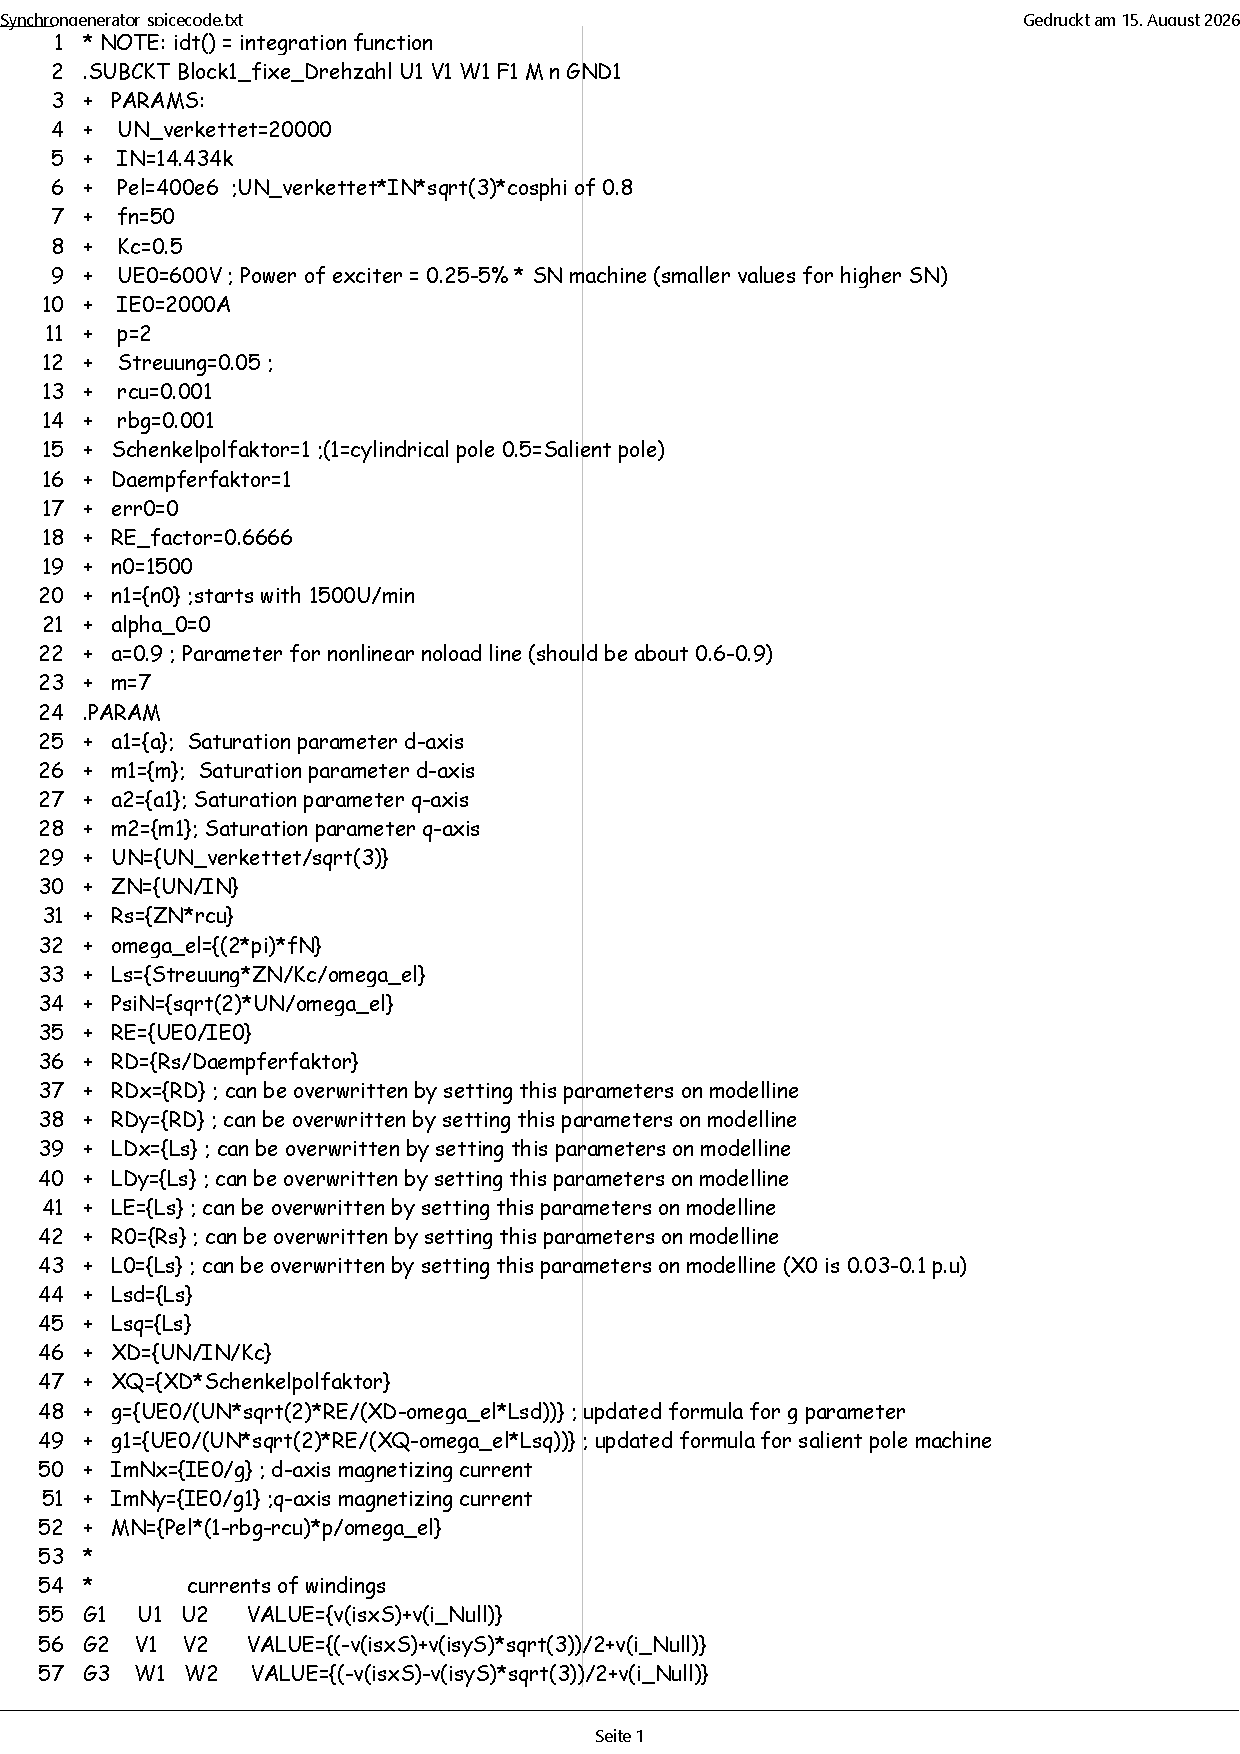
\includegraphics[width=0.90\textwidth]{figures/Synchronmaschine_SpiceCode_1.pdf}
%	\caption{Spice Listing for synchronous machine model page1 of 2}
%	\label{fig:Synchronous machine listing1}
%\end{figure}
%
%\begin{figure}[H]
%	\centering
%	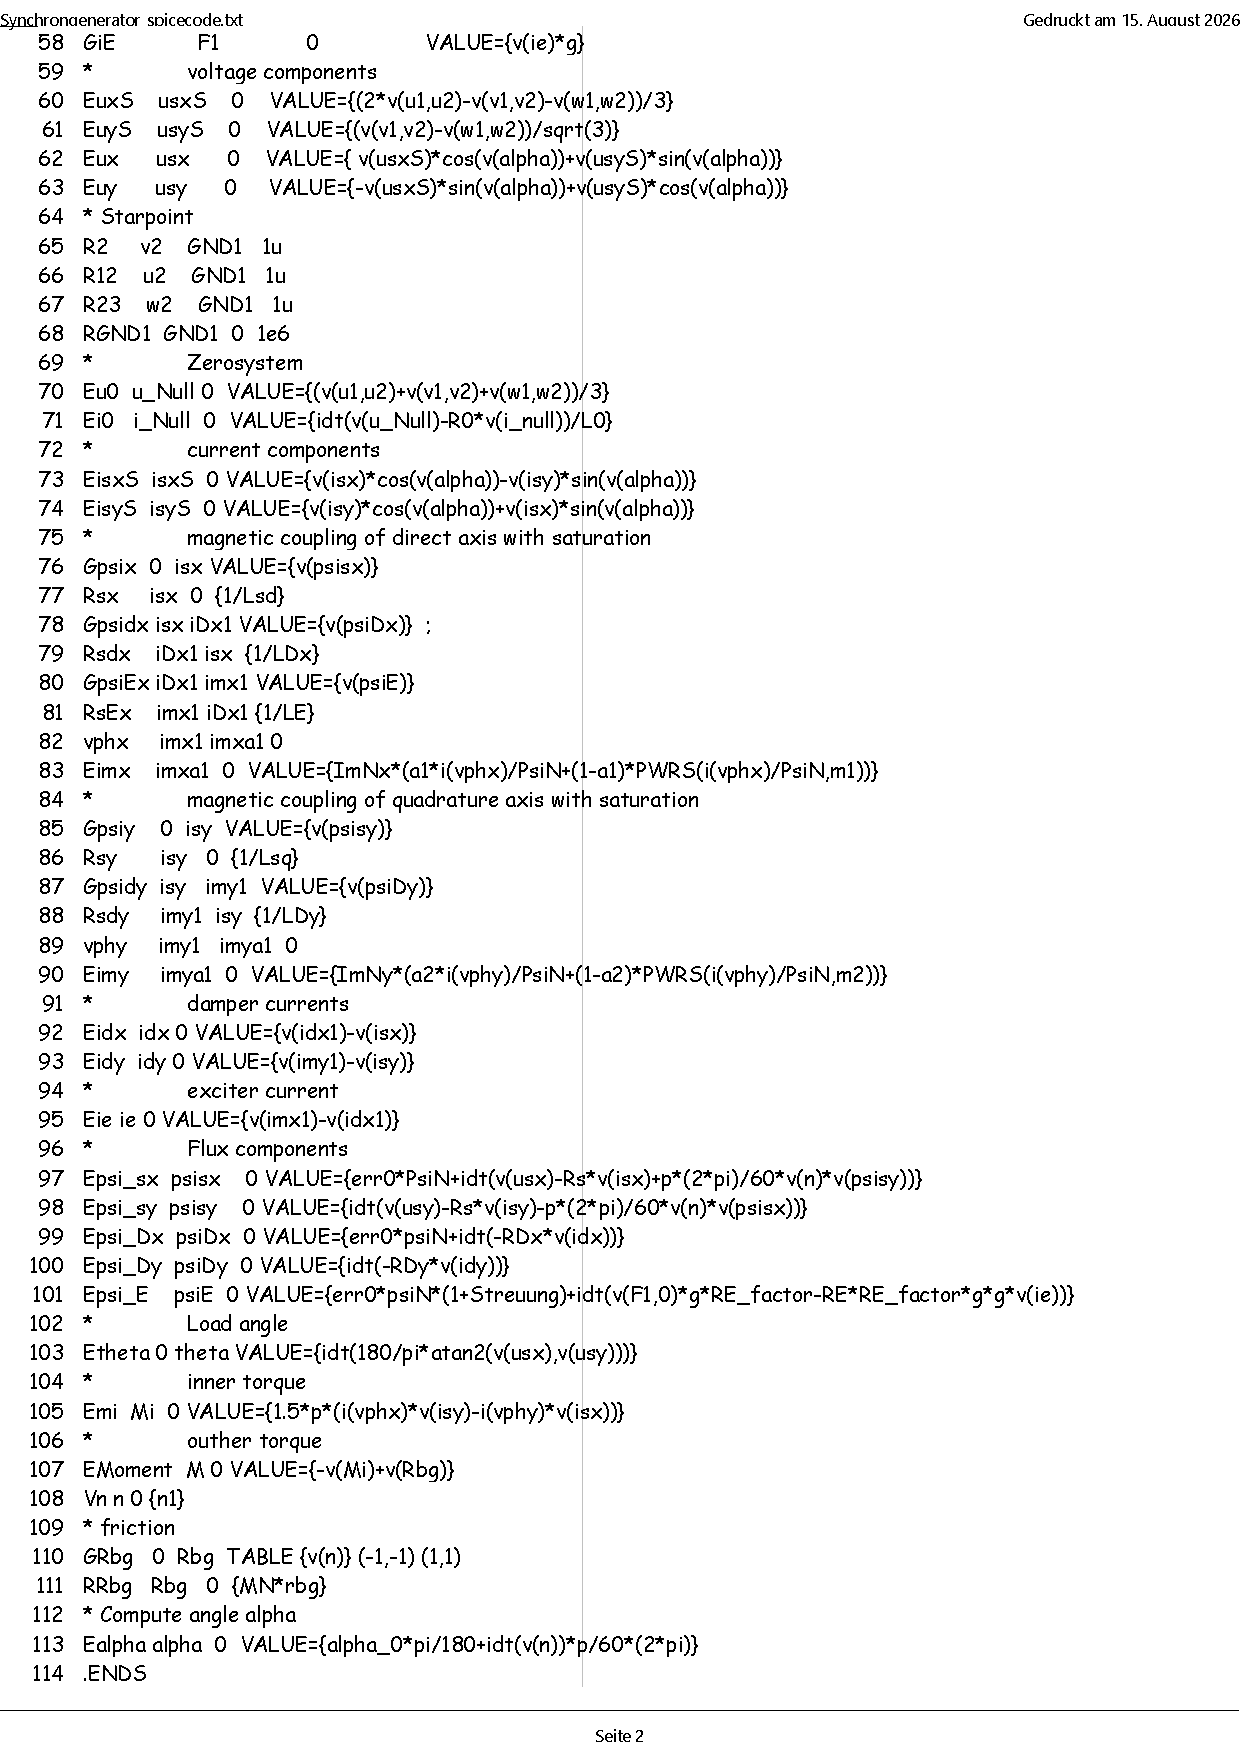
\includegraphics[width=0.90\textwidth]{figures/Synchronmaschine_SpiceCode_2.pdf}
%	\caption{Spice Listing for synchronous machine model page2 of 2}
%	\label{fig:Synchronous machine listing2}
%\end{figure}

\begin{figure}[H]
	\centering
	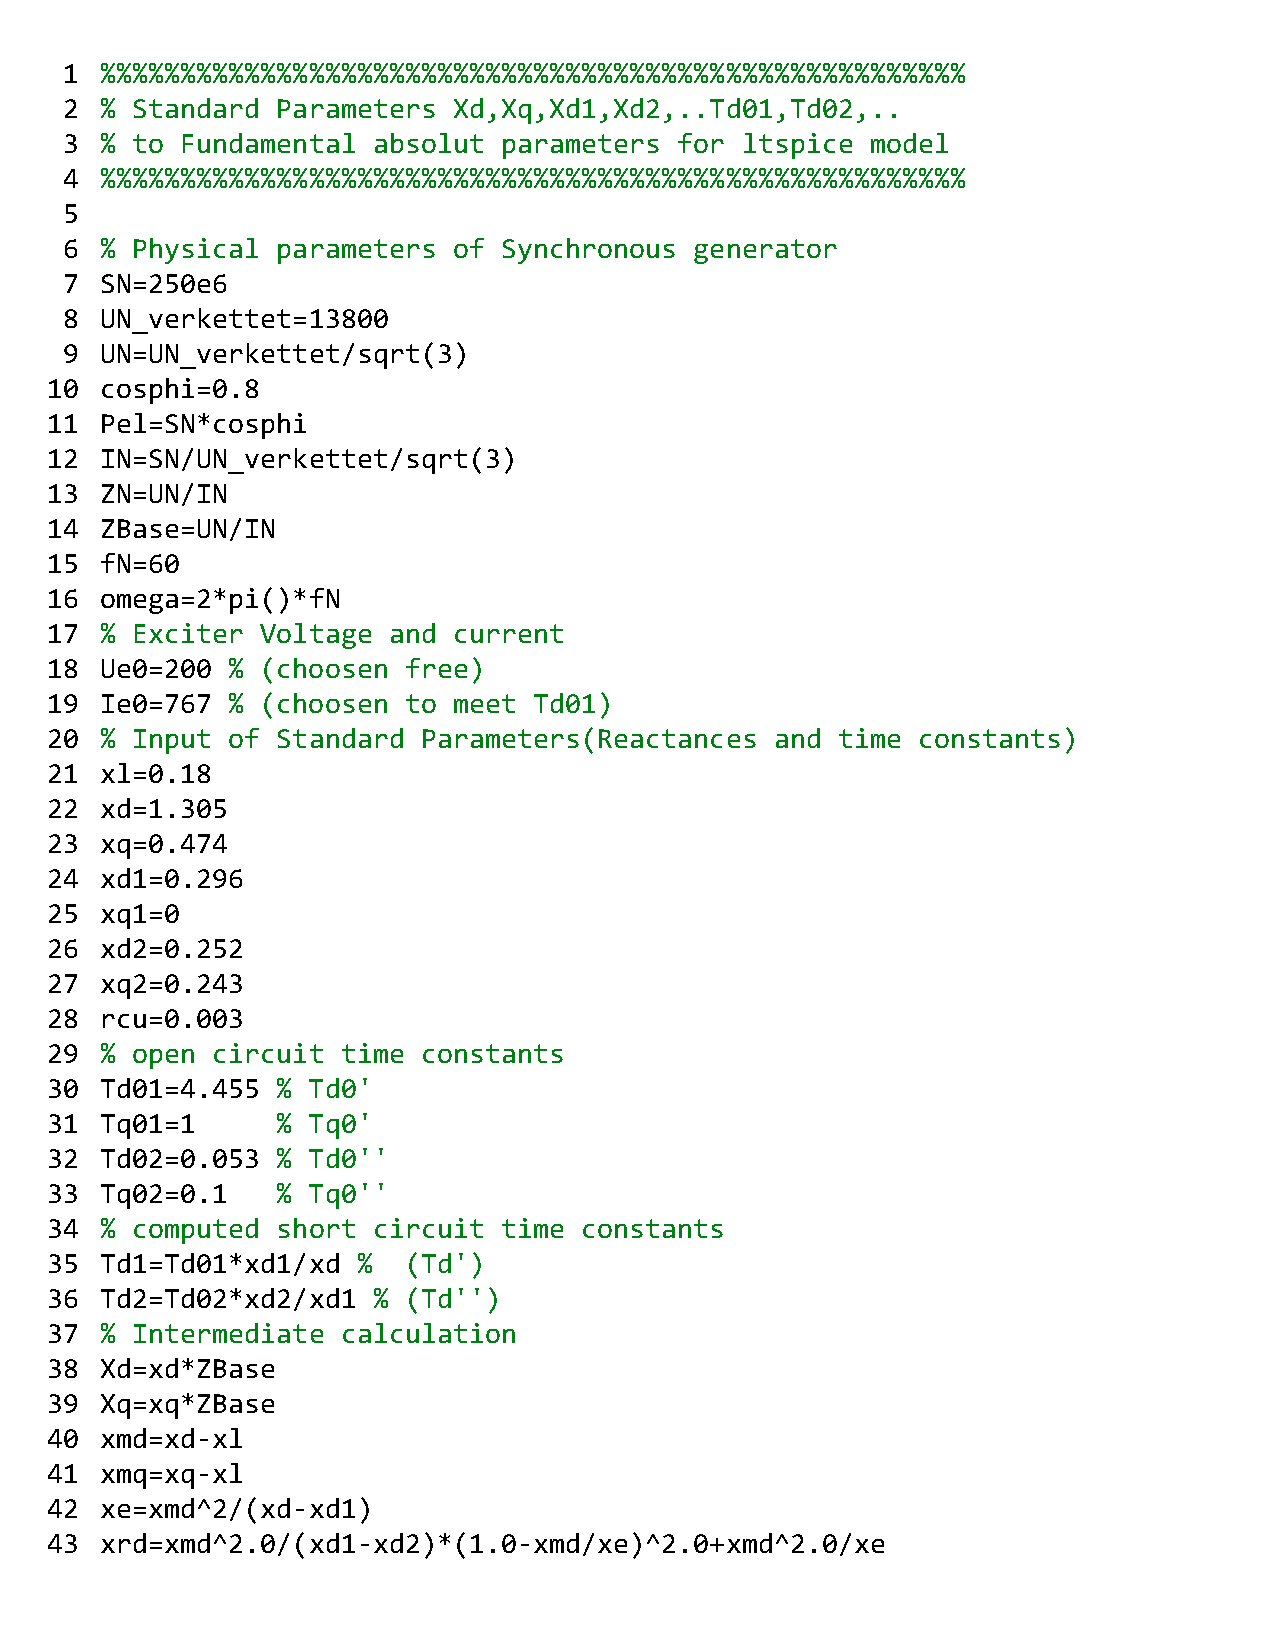
\includegraphics[width=0.90\textwidth]{figures/Matlab_Standardparameters_to_Fundamentalparameters 1.pdf}
	\caption{MATLAB code for converting standard machine parameters to fundamental model parameters}
	\label{fig:Standard to fundamental parameters}
\end{figure}

\begin{figure}[H]
	\centering
	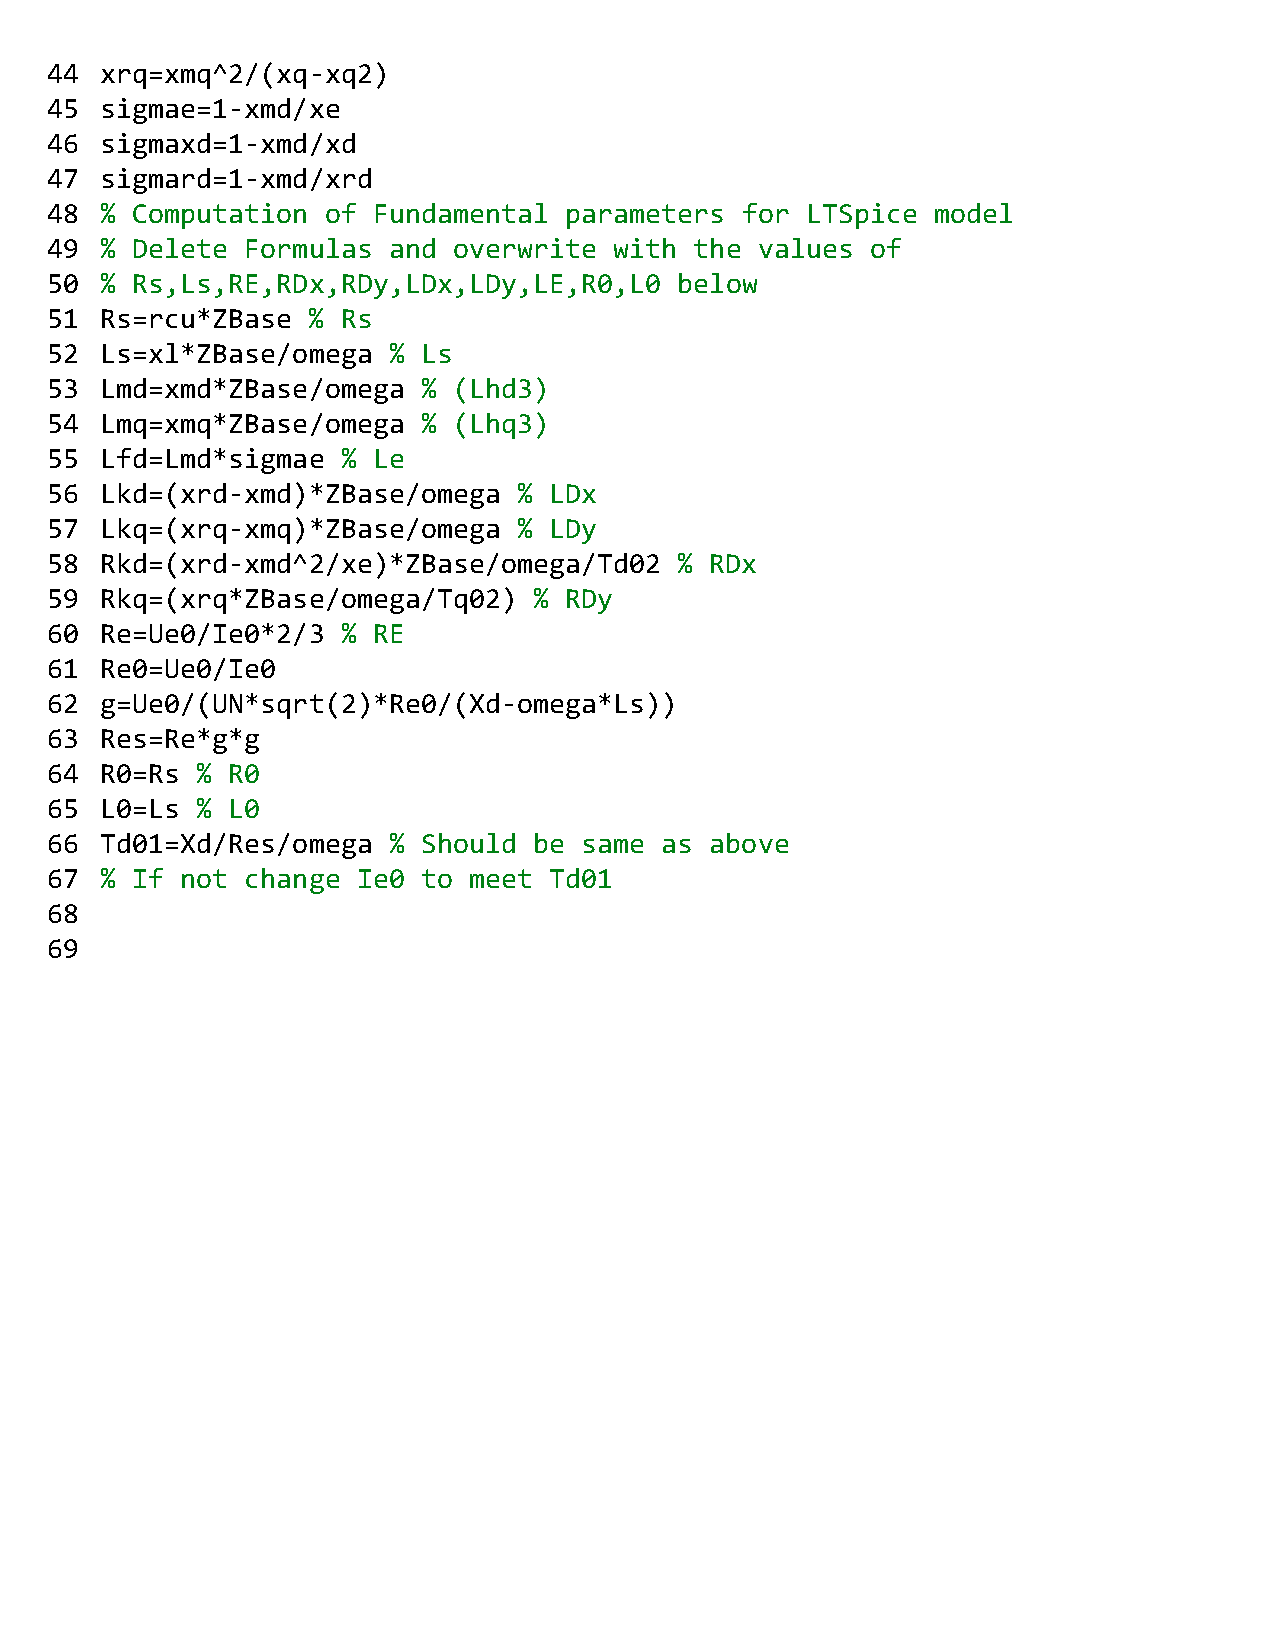
\includegraphics[width=0.90\textwidth]{figures/Matlab_Standardparameters_to_Fundamentalparameters 2.pdf}
	\caption{MATLAB code for converting standard machine parameters to fundamental model parameters}
	\label{fig:Standard to fundamental parameters}
\end{figure}	
		




\formulasheettitle{Transformer Model}%
  {Formula sheet for a three-phase two-winding transformer}
	\begin{noteBox}
		\textbf{Notation.} Indices $k=1,2,3$ identify the transformer legs or phases;
		$p$ and $s$ denote the primary and secondary windings. Uppercase $U$ and $I$
		denote electrical quantities, $\Phi$ the magnetic flux, $\Psi=N\Phi$ the flux
		linkage, and $\Theta=NI$ the magnetomotive force. The example uses vector group
		$\mathrm{Yy0}$.
	\end{noteBox}
	
	\begin{formulaBox}{Transformer-leg equations}
		For each leg $k\in\{1,2,3\}$, the reluctance associated with the iron-loss
		resistance is
		\begin{equation}
			\Rmag_{R\mathrm{Fe}}=\frac{N_1^2}{R_{\mathrm{Fe}}}.
		\end{equation}
		The nonlinear magnetizing characteristic is represented by
		\begin{equation}
			\Theta_{\mu k}=N_1 I_{\mu N}
			\left[
			a\frac{\Phi_k}{\Phi_N}
			+(1-a)\left(\frac{\Phi_k}{\Phi_N}\right)^m
			\right],
			\qquad k=1,2,3.
		\end{equation}
		Equivalently, the magnetizing current of one leg is
		\begin{equation}
			I_{\mu k}=I_{\mu N}
			\left[
			a\frac{\Phi_k}{\Phi_N}
			+(1-a)\left(\frac{\Phi_k}{\Phi_N}\right)^m
			\right].
		\end{equation}
	\end{formulaBox}
	
	\begin{formulaBox}{Primary-winding equations}
		For every phase $k$,
		\begin{align}
			\Phi_{kp}
			&=\frac{\Psi_{kp}}{N_1}
			=\frac{1}{N_1}\int\!\left(U_{kp}-R_1I_{kp}\right)\diff t,
			& I_{kp}&=\frac{\Theta_k}{N_1}.
		\end{align}
		Written separately for the three phases, this relation applies for
		$k=1$, $2$, and $3$ with the corresponding phase quantities.
	\end{formulaBox}
	
	\begin{formulaBox}{Secondary-winding equations}
		For every phase $k$,
		\begin{align}
			\Phi_{ks}
			&=\frac{\Psi_{ks}}{N_2}
			=\frac{1}{N_2}\int\!\left(U_{ks}-R_2I_{ks}\right)\diff t,
			& I_{ks}&=\frac{\Theta_k}{N_2}.
		\end{align}
		The voltage and current reference directions must be chosen consistently with
		the winding polarities used in the circuit model.
	\end{formulaBox}
	
	\newpage
	\thispagestyle{scrheadings}
	
	\begin{formulaBox}{Common core flux and winding flux linkages}
		For ideal magnetic coupling of the windings on each leg,
		\begin{equation}
			\Phi_{kp}=\Phi_{ks}=\Phi_k,
			\qquad k=1,2,3.
		\end{equation}
		The corresponding flux linkages are
		\begin{equation}
			\Psi_{kp}=N_1\Phi_k,
			\qquad
			\Psi_{ks}=N_2\Phi_k.
		\end{equation}
		Thus, in general,
		\begin{equation}
			\Psi_{kp}\ne\Psi_{ks}\quad\text{when}\quad N_1\ne N_2,
		\end{equation}
		even though both windings link the same core flux $\Phi_k$.
	\end{formulaBox}
	
	\begin{formulaBox}{Leakage-flux branch}
		With $\Rmag_{\Phi\sigma}$ denoting the equivalent magnetic reluctance of the
		leakage path,
		\begin{equation}
			\Phi_{k\sigma}=\frac{\Theta_k}{\Rmag_{\Phi\sigma}},
			\qquad k=1,2,3.
		\end{equation}
		For a leakage inductance $L_{1\sigma}$ referred to the primary winding,
		\begin{equation}
			L_{1\sigma}=\frac{N_1^2}{\Rmag_{\Phi\sigma}}
			\qquad\Longleftrightarrow\qquad
			\Rmag_{\Phi\sigma}=\frac{N_1^2}{L_{1\sigma}}.
		\end{equation}
	\end{formulaBox}
	
	\begin{formulaBox}{Tank representation}
		The tank is represented by an additional magnetic reluctance $\Rmag_{\mathrm{tank}}$.
		The source text recommends the following approximate choices:
		\begin{align}
			\Rmag_{\mathrm{tank}}
			&\approx (0.1\ldots0.01)\frac{N_1^2}{L_{1\sigma}},
			&&\text{rough initial estimate: 10–100 times the leakage inductance},\\
			\Rmag_{\mathrm{tank}}
			&\approx 10^5\ldots10^6,
			&&\text{tank magnetic reluctance in the model units},\\
			\Rmag_{\mathrm{tank}}
			&\approx 10^{20},
			&&\text{tank branch absent (practically open)}.
		\end{align}
	\end{formulaBox}
	
	
	\newpage
	\thispagestyle{scrheadings}
	
%	\begin{formulaBox}{Rated data: 300 MVA, 400 kV / 120 kV, 50 Hz}
%		\renewcommand{\arraystretch}{\formulaTableStretch}
%		\begin{tabularx}{\textwidth}{>{\bfseries\(}l<{\)} >{\(}l<{\)} X}
%			\toprule
%			\text{Symbol} & \text{Value} & \textbf{Meaning} \\
%			\midrule
%			S_N & 300\times10^6\ \mathrm{VA} & Three-phase rated apparent power \\
%			U_{1N,LL} & 400\times10^3\ \mathrm{V} & Primary rated line-to-line voltage \\
%			U_{2N,LL} & 120\times10^3\ \mathrm{V} & Secondary rated line-to-line voltage \\
%			f_N & 50\ \mathrm{Hz} & Rated frequency \\
%			N_1 & 1000 & Primary number of turns \\
%			u_R & 0.002 & Resistive part of relative short-circuit voltage \\
%			u_X & 0.2 & Inductive part of relative short-circuit voltage \\
%			i_0 & 0.0006 & Relative no-load current \\
%			p_0 & 0.0004 & Relative no-load loss, with $p_0<i_0$ \\
%			a & 0.75 & Linear weighting in the magnetizing characteristic \\
%			m & 9 & Exponent of the nonlinear magnetizing term \\
%			\bottomrule
%		\end{tabularx}
%	\end{formulaBox}

	\begin{formulaBox}{Transformer main data:}
			\renewcommand{\arraystretch}{\formulaTableStretch}
			\begin{tabularx}{\textwidth}{>{\bfseries\(}l<{\)} >{\text{}}l X}
					\toprule
					\text{Symbol} & \textbf{Meaning} \\
					\midrule
					S_N & Three-phase rated apparent power \\
					U_{1N,LL} & Primary rated line-to-line voltage \\
					U_{2N,LL} & Secondary rated line-to-line voltage \\
					f_N & Rated frequency \\
					N_1 & Primary number of turns \\
					u_R & Resistive part of relative short-circuit voltage \\
					u_X & Inductive part of relative short-circuit voltage \\
					i_0 & Relative no-load current \\
					p_0 & Relative no-load loss, with $p_0<i_0$ \\
					a & Linear weighting in the magnetizing characteristic \\
					m & Exponent of the nonlinear magnetizing term \\
					\bottomrule
			\end{tabularx}
	\end{formulaBox}
	
	\begin{formulaBox}{Per-leg quantities for vector group $\mathrm{Yy0}$}
		The three-phase values are first converted to one transformer leg:
		\begin{align}
			S_{N,\mathrm{leg}} &= \frac{S_N}{3}, &
			U_{1N} &= \frac{U_{1N,LL}}{\sqrt{3}}, &
			U_{2N} &= \frac{U_{2N,LL}}{\sqrt{3}},\\
			I_{1N} &= \frac{S_{N,\mathrm{leg}}}{U_{1N}}, &
			Z_{1N} &= \frac{U_{1N}}{I_{1N}}, &
			\omega_N &= 2\pi f_N.
		\end{align}
	\end{formulaBox}
	
	\begin{formulaBox}{Winding and iron-loss parameters}
		The short-circuit impedance is split equally between the two windings and
		referred initially to the primary side:
		\begin{align}
			R_1 &= \frac{Z_{1N}u_R}{2}, &
			L_{1\sigma} &= \frac{Z_{1N}u_X}{2\omega_N},\\
			R_{\mathrm{Fe}} &= \frac{U_{1N}^2}{p_0S_{N,\mathrm{leg}}}, &
			\Rmag_{R\mathrm{Fe}} &= \frac{N_1^2}{R_{\mathrm{Fe}}},\\
			N_2 &= N_1\frac{U_{2N}}{U_{1N}}, &
			R_2 &= R_1\left(\frac{N_2}{N_1}\right)^2,\\
			\Rmag_{\Phi\sigma} &= \frac{N_1^2}{L_{1\sigma}}. &&
		\end{align}
	\end{formulaBox}
	
	\newpage
	\thispagestyle{scrheadings}
	
	\begin{formulaBox}{Magnetizing branch and rated flux}
		From the no-load current and no-load losses,
		\begin{align}
			X_h &= \frac{U_{1N}^2}
			{S_{N,\mathrm{leg}}\sqrt{i_0^2-p_0^2}},\\
			I_\mu &= \frac{U_{1N}}{X_h},\\
			I_{\mu N} &= \sqrt{2}\,I_\mu,\\
			\Phi_N &= \frac{\sqrt{2}\,U_{1N}}{\omega_NN_1}.
		\end{align}
		The nonlinear characteristic then becomes
		\begin{equation}
			I_\mu(\Phi)=I_{\mu N}
			\left[
			a\frac{\Phi}{\Phi_N}
			+(1-a)\left(\frac{\Phi}{\Phi_N}\right)^m
			\right].
		\end{equation}
	\end{formulaBox}
	
	\begin{formulaBox}{Parameter definitions}
		\renewcommand{\arraystretch}{\formulaTableStretch}
		\begin{tabularx}{\textwidth}{>{\bfseries\(}l<{\)} X}
			\toprule
			\text{Symbol} & \textbf{Meaning} \\
			\midrule
			\Theta_k & Magnetomotive force of leg $k$ \\
			\Phi_k,\ \Phi_{k\sigma} & Main and leakage fluxes of leg $k$ \\
			\Psi_{kp},\ \Psi_{ks} & Primary and secondary flux linkages \\
			\Rmag_{R\mathrm{Fe}} & Magnetic reluctance associated with the iron-loss branch \\
			\Rmag_{\Phi\sigma} & Equivalent leakage-path reluctance \\
			\Rmag_{\mathrm{tank}} & Tank-path magnetic reluctance \\
			R_1,\ R_2 & Primary and secondary winding resistances \\
			R_{\mathrm{Fe}} & Equivalent iron-loss resistance \\
			L_{1\sigma} & Primary-referred leakage inductance \\
			X_h & Main magnetizing reactance \\
			I_{\mu N},\ \Phi_N & Rated peak magnetizing current and rated peak flux \\
			a,\ m & Shape parameters of the nonlinear magnetization curve \\
			\bottomrule
		\end{tabularx}
	\end{formulaBox}
	
	\begin{noteBox}
		\textbf{Implementation notes.} The time integrals may be implemented with
		behavioural sources in LTspice. When forming the winding equations, verify the
		chosen voltage polarities, current reference directions, initial flux, and the
		sign of each magnetomotive-force contribution. The numerical tank-reluctance
		range is model- and unit-dependent and should be validated against the intended
		zero-sequence behaviour.
	\end{noteBox}
	
	\vfill
%	{\small\color{muted}\sffamily
%		Typeset from the supplied transformer-model notes. English wording and notation
%		have been standardized; explicitly identified dimensional inconsistencies in
%		the source have been corrected.}

	\begin{formulaBox}{Rated data: 300 MVA, 400 kV / 120 kV, 50 Hz}
			\renewcommand{\arraystretch}{\formulaTableStretch}
			\begin{tabularx}{\textwidth}{>{\bfseries\(}l<{\)} >{\(}l<{\)} X}
					\toprule
					\text{Symbol} & \text{Value} & \textbf{Meaning} \\
					\midrule
					S_N & 300\times10^6\ \mathrm{VA} & Three-phase rated apparent power \\
					U_{1N,LL} & 400\times10^3\ \mathrm{V} & Primary rated line-to-line voltage \\
					U_{2N,LL} & 120\times10^3\ \mathrm{V} & Secondary rated line-to-line voltage \\
					f_N & 50\ \mathrm{Hz} & Rated frequency \\
					N_1 & 1000 & Primary number of turns \\
					u_R & 0.002 & Resistive part of relative short-circuit voltage \\
					u_X & 0.2 & Inductive part of relative short-circuit voltage \\
					i_0 & 0.0006 & Relative no-load current \\
					p_0 & 0.0004 & Relative no-load loss, with $p_0<i_0$ \\
					a & 0.75 & Linear weighting in the magnetizing characteristic \\
					m & 9 & Exponent of the nonlinear magnetizing term \\
					\bottomrule
			\end{tabularx}
	\end{formulaBox}
	
% LaTeX fragment for direct insertion into a book chapter.
% Required definitions/packages are provided by the central preamble:
% formulaBox, noteBox, amsmath, booktabs, tabularx, siunitx.

\begin{noteBox}
	\textbf{Assumptions.}
	The calculation uses a balanced per-phase equivalent circuit for vector group
	$\mathrm{Yy0}$. The total short-circuit resistance and leakage reactance are
	split equally between the primary winding and the secondary winding referred
	to the primary side. All magnetizing-branch quantities are initially referred
	to the \SI{400}{\kilo\volt} side.
\end{noteBox}

\begin{formulaBox}{Per-leg rated quantities}
	The three-phase rated values are converted to one transformer leg:
	\begin{align}
		S_{N,\mathrm{leg}}
		&=\frac{S_N}{3}
		=\frac{\SI{300}{\mega\volt\ampere}}{3}
		=\SI{100}{\mega\volt\ampere},\\
		U_{1N}
		&=\frac{U_{1N,LL}}{\sqrt{3}}
		=\frac{\SI{400}{\kilo\volt}}{\sqrt{3}}
		=\SI{230.940}{\kilo\volt},\\
		U_{2N}
		&=\frac{U_{2N,LL}}{\sqrt{3}}
		=\frac{\SI{120}{\kilo\volt}}{\sqrt{3}}
		=\SI{69.282}{\kilo\volt},\\
		I_{1N}
		&=\frac{S_{N,\mathrm{leg}}}{U_{1N}}
		=\SI{433.013}{\ampere},\\
		Z_{1N}
		&=\frac{U_{1N}}{I_{1N}}
		=\frac{U_{1N,LL}^{2}}{S_N}
		=\SI{533.333}{\ohm},\\
		\omega_N
		&=2\pi f_N
		=\SI{314.159}{\radian\per\second}.
	\end{align}
	
	The turns ratio and secondary number of turns are
	\begin{align}
		u=\frac{N_1}{N_2}
		&=\frac{U_{1N}}{U_{2N}}
		=\frac{400}{120}
		=3.33333,\\
		N_2&=N_1\frac{U_{2N}}{U_{1N}}
		=1000\frac{120}{400}
		=\boxed{300}.
	\end{align}
\end{formulaBox}

\begin{formulaBox}{Winding parameters}
	The total short-circuit resistance and leakage reactance referred to the
	primary side are
	\begin{align}
		R_k'&=u_R Z_{1N}
		=0.002\cdot\SI{533.333}{\ohm}
		=\SI{1.06667}{\ohm},\\
		X_{k\sigma}'&=u_X Z_{1N}
		=0.2\cdot\SI{533.333}{\ohm}
		=\SI{106.667}{\ohm},\\
		L_{k\sigma}'&=\frac{X_{k\sigma}'}{\omega_N}
		=\SI{0.339531}{\henry}.
	\end{align}
	
	With equal division between the two windings,
	\begin{align}
		R_1=R_2'
		&=\frac{R_k'}{2}
		=\boxed{\SI{0.533333}{\ohm}},\\
		L_{1\sigma}=L_{2\sigma}'
		&=\frac{L_{k\sigma}'}{2}
		=\boxed{\SI{0.169765}{\henry}}.
	\end{align}
	
	The actual secondary-side parameters follow from
	$(N_2/N_1)^2=0.09$:
	\begin{align}
		R_2&=R_2'\left(\frac{N_2}{N_1}\right)^2
		=\SI{0.533333}{\ohm}\cdot0.09
		=\boxed{\SI{0.048000}{\ohm}},\\
		L_{2\sigma}&=L_{2\sigma}'\left(\frac{N_2}{N_1}\right)^2
		=\SI{0.169765}{\henry}\cdot0.09
		=\boxed{\SI{0.0152789}{\henry}}.
	\end{align}
	
	For the magnetic-circuit leakage representation,
	\begin{equation}
		\Rmag_{\Phi\sigma}
		=\frac{N_1^2}{L_{1\sigma}}
		=\frac{1000^2}{\SI{0.169765}{\henry}}
		=\boxed{\SI{5.89049e6}{\per\henry}}.
	\end{equation}
\end{formulaBox}

\begin{formulaBox}{Iron-loss parameters}
	The total rated no-load loss is
	\begin{equation}
		P_0=p_0S_N
		=0.0004\cdot\SI{300}{\mega\volt\ampere}
		=\SI{120}{\kilo\watt}.
	\end{equation}
	
	Thus, each transformer leg represents
	\SI{40}{\kilo\watt} of iron loss. The primary-referred iron-loss resistance is
	\begin{align}
		R_{\mathrm{Fe}}
		&=\frac{U_{1N}^{2}}{p_0S_{N,\mathrm{leg}}}\\
		&=\frac{(\SI{230.940}{\kilo\volt})^2}
		{0.0004\cdot\SI{100}{\mega\volt\ampere}}
		=\boxed{\SI{1.33333}{\mega\ohm}}.
	\end{align}
	
	The corresponding RMS iron-loss current per phase is
	\begin{equation}
		I_{\mathrm{Fe}}
		=\frac{U_{1N}}{R_{\mathrm{Fe}}}
		=\boxed{\SI{0.173205}{\ampere}}.
	\end{equation}
	
	In the magnetic-circuit representation used by the transformer model,
	\begin{equation}
		\Rmag_{R\mathrm{Fe}}
		=\frac{N_1^2}{R_{\mathrm{Fe}}}
		=\frac{1000^2}{\SI{1.33333e6}{\ohm}}
		=\boxed{0.750000}.
	\end{equation}
\end{formulaBox}

\begin{formulaBox}{Magnetizing branch and rated flux}
	The rated RMS no-load current is
	\begin{equation}
		I_0=i_0I_{1N}
		=0.0006\cdot\SI{433.013}{\ampere}
		=\SI{0.259808}{\ampere}.
	\end{equation}
	
	After subtracting the active iron-loss component vectorially, the RMS
	magnetizing current is
	\begin{align}
		I_\mu
		&=I_{1N}\sqrt{i_0^2-p_0^2}\\
		&=\SI{433.013}{\ampere}
		\sqrt{0.0006^2-0.0004^2}
		=\boxed{\SI{0.193649}{\ampere}}.
	\end{align}
	
	The magnetizing reactance and inductance referred to the primary side are
	\begin{align}
		X_h
		&=\frac{U_{1N}}{I_\mu}
		=\frac{U_{1N}^2}
		{S_{N,\mathrm{leg}}\sqrt{i_0^2-p_0^2}}
		=\boxed{\SI{1.19257}{\mega\ohm}},\\
		L_h
		&=\frac{X_h}{\omega_N}
		=\boxed{\SI{3.79607e3}{\henry}}.
	\end{align}
	
	The peak magnetizing current used in the nonlinear characteristic is
	\begin{equation}
		I_{\mu N}=\sqrt{2}\,I_\mu
		=\boxed{\SI{0.273861}{\ampere}}.
	\end{equation}
	
	For a sinusoidal phase voltage, the rated peak core flux is
	\begin{align}
		\Phi_N
		&=\frac{\sqrt{2}\,U_{1N}}{\omega_NN_1}\\
		&=\frac{\sqrt{2}\cdot\SI{230.940}{\kilo\volt}}
		{\SI{314.159}{\radian\per\second}\cdot1000}
		=\boxed{\SI{1.03960}{\weber}}.
	\end{align}
	
	With $a=0.75$ and $m=9$, the numerical magnetizing characteristic becomes
	\begin{equation}
		I_\mu(\Phi)
		=\SI{0.273861}{\ampere}
		\left[
		0.75\frac{\Phi}{\SI{1.03960}{\weber}}
		+0.25\left(\frac{\Phi}{\SI{1.03960}{\weber}}\right)^9
		\right].
	\end{equation}
\end{formulaBox}

\begin{formulaBox}{Calculated parameter summary}
	\renewcommand{\arraystretch}{\formulaTableStretch}
	\begin{tabularx}{\textwidth}{>{\bfseries\(}l<{\)} >{\(}l<{\)} X}
		\toprule
		\text{Parameter} & \text{Calculated value} & \textbf{Reference} \\
		\midrule
		N_2 & 300 & Secondary number of turns \\
		R_1 & \SI{0.533333}{\ohm} & Primary winding resistance \\
		L_{1\sigma} & \SI{0.169765}{\henry} & Primary leakage inductance \\
		R_2' & \SI{0.533333}{\ohm} & Secondary resistance referred to primary \\
		L_{2\sigma}' & \SI{0.169765}{\henry} & Secondary leakage inductance referred to primary \\
		R_2 & \SI{0.048000}{\ohm} & Actual secondary resistance \\
		L_{2\sigma} & \SI{0.0152789}{\henry} & Actual secondary leakage inductance \\
		R_{\mathrm{Fe}} & \SI{1.33333}{\mega\ohm} & Iron-loss resistance, primary-referred \\
		X_h & \SI{1.19257}{\mega\ohm} & Magnetizing reactance, primary-referred \\
		L_h & \SI{3.79607e3}{\henry} & Linear magnetizing inductance \\
		I_{\mu N} & \SI{0.273861}{\ampere} & Rated peak magnetizing current \\
		\Phi_N & \SI{1.03960}{\weber} & Rated peak core flux \\
		\Rmag_{R\mathrm{Fe}} & 0.750000 & Iron-loss magnetic-model parameter \\
		\Rmag_{\Phi\sigma} & \SI{5.89049e6}{\per\henry} & Leakage-path magnetic parameter \\
		\bottomrule
	\end{tabularx}
\end{formulaBox}


\begin{widefigure}{Electrical and magnetic model of a three-phase Yy0 transformer with a three-leg core}{fig:schematic1}
	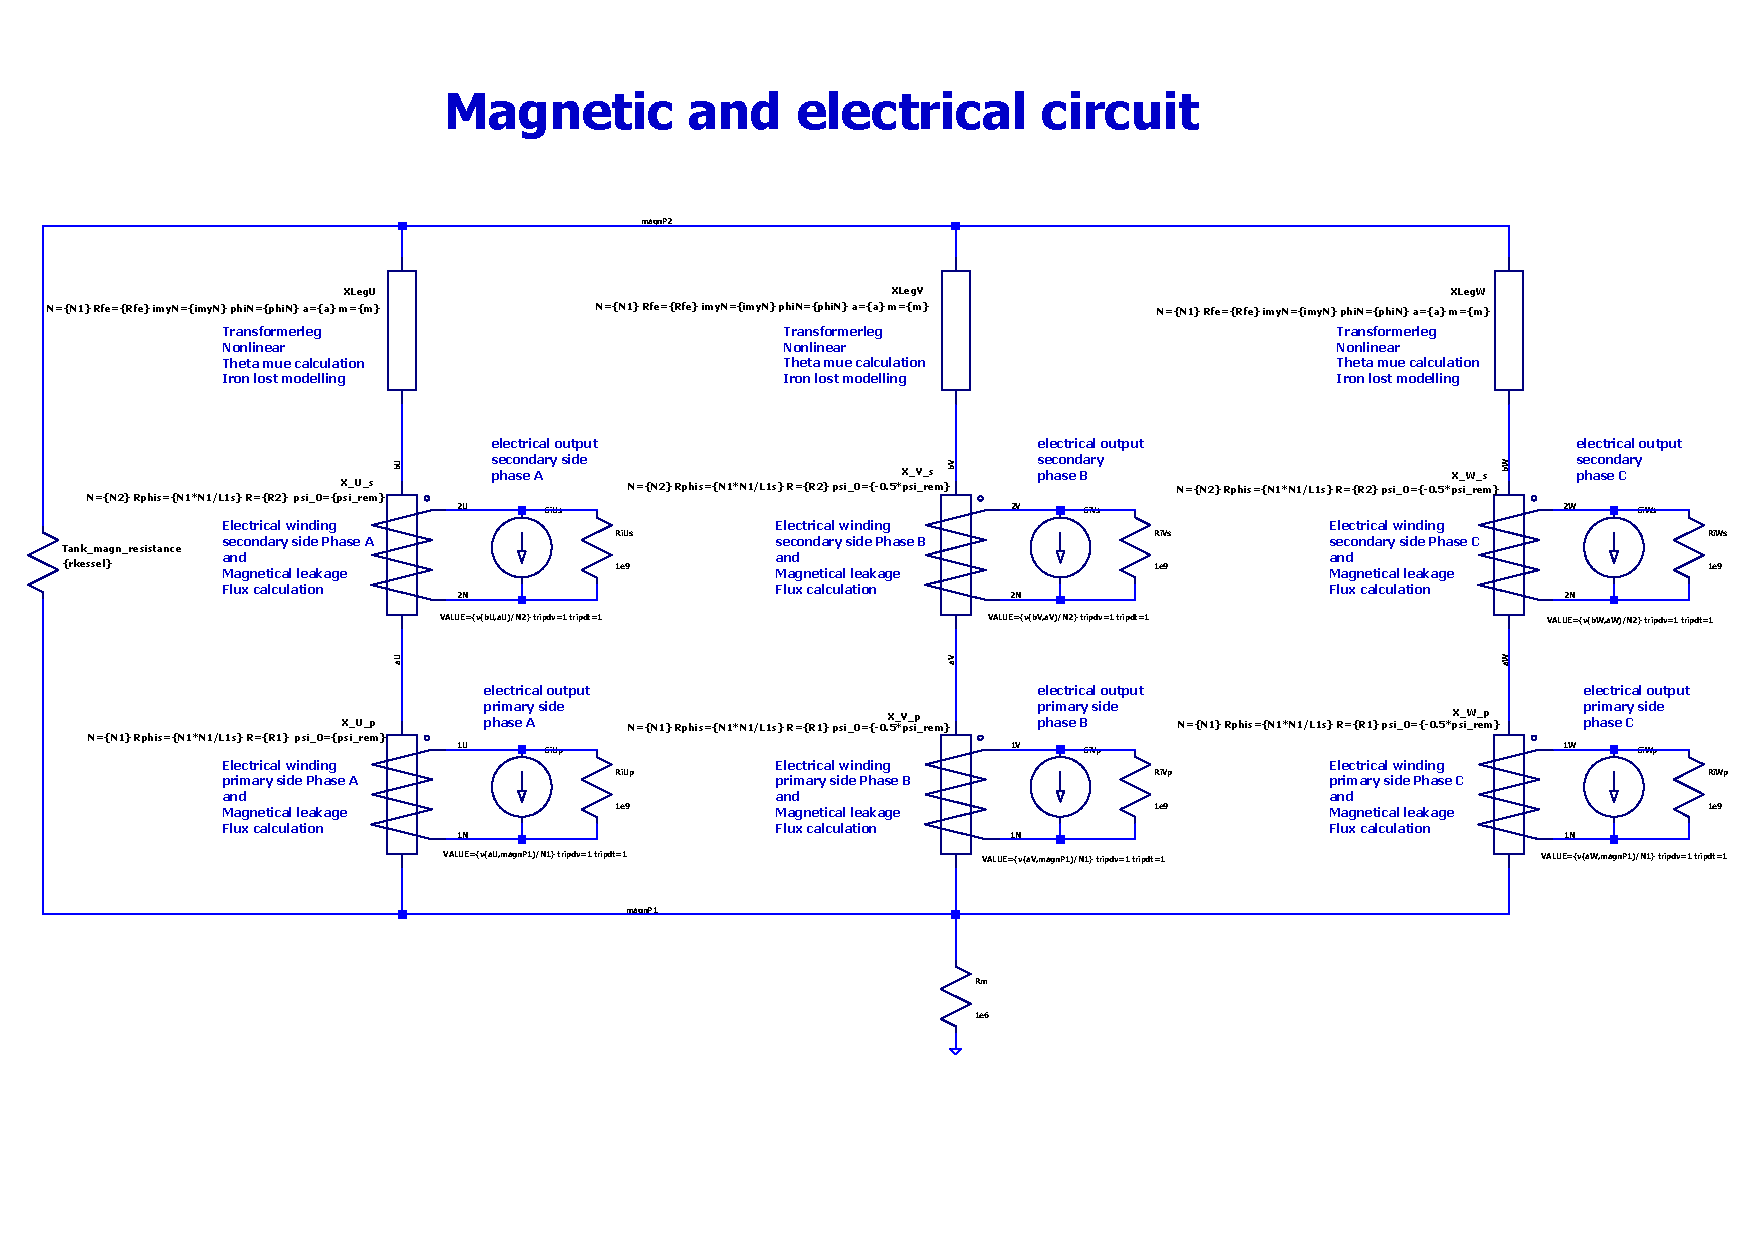
\includegraphics[width=1.5\textwidth]{figures/trafo_Yy_hierarchical_designed.pdf}
\end{widefigure}

%\begin{figure}[H]
%	\centering
%	\includegraphics[width=0.99\textwidth]{figures/Transformer_and_shunt_reactor_AC_Schematic}
%	\caption{Schematic for the Transformer and shunt reactor circuit.}
%	\label{fig:Transformer_and_shunt_reactor_AC_Schematic}
%\end{figure}


\begin{figure}[H]
	\centering
	\includegraphics[width=0.90\textwidth]{figures/winding_and_transformerleg.pdf}
	\caption{One winding and one leg of the transformer model}
	\label{fig:Transformer_and_shunt_reactor_AC_Waveform}
\end{figure}

%\begin{figure}[H]
%	\centering
%	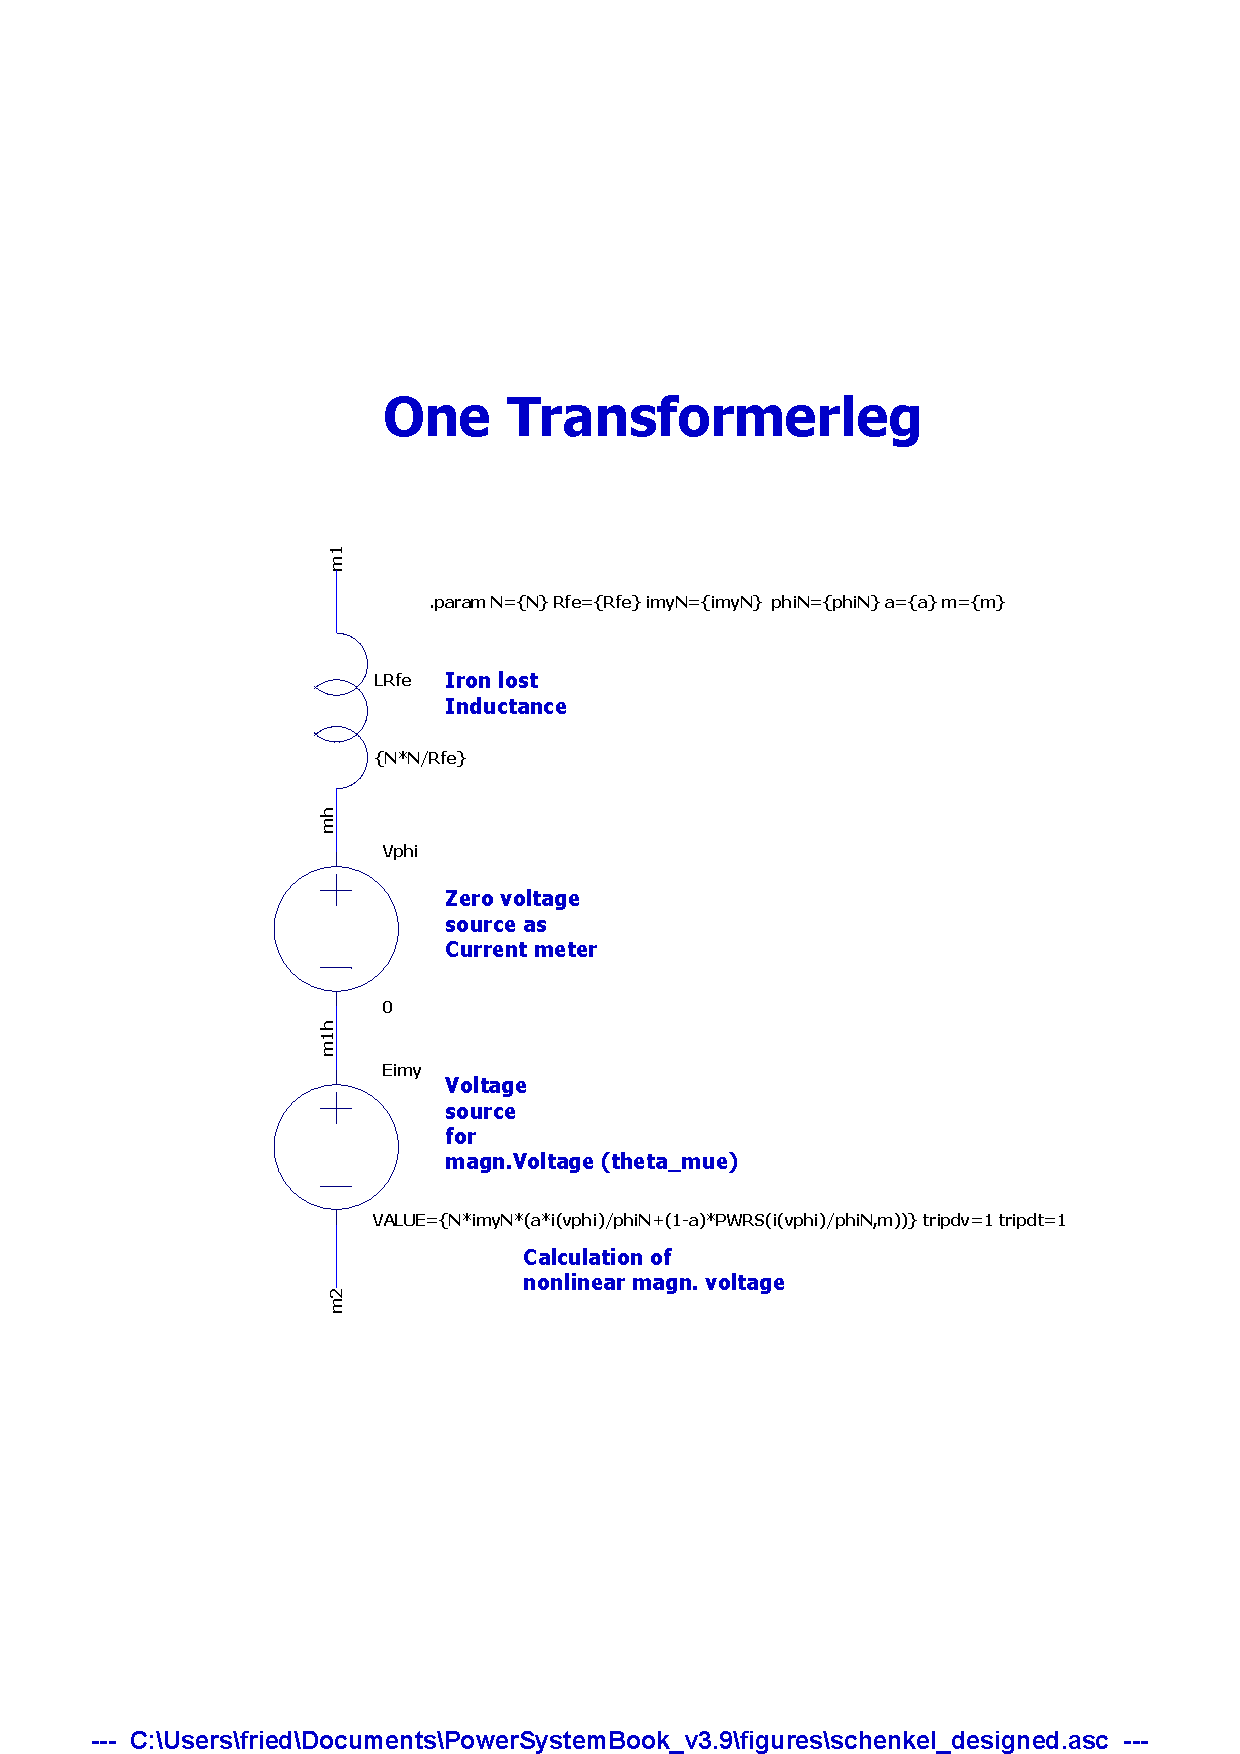
\includegraphics[width=0.90\textwidth]{figures/schenkel_designed.pdf}
%	\caption{One Leg of the transformer model}
%	\label{fig:Transformer_and_shunt_reactor_AC_Waveform}
%\end{figure}

\pagebreak

\begin{lstlisting}[style=LTspice,caption={Behavioral implementation of a three-phase transformer.},label={lst:Three phase transformer}]

1 .SUBCKT RUYy0_400k_120k_300MVA 1U 1V 1W 1N 2U 2V 2W 2N
2 + PARAMS:
3 + SN=300e6
4 + U1Nenn=400e3
5 + U20=120e3
6 + fn={fn1}
7 + N1=1000
8 + uR=0.002
9 + uX=0.2
10 + i0=0.0006
11 + p0=0.0004
12 + a=0.75 ; FS
13 + m=9;FS
14 + psi_0=0 ; Remanence-parameter 0,1,-1
15 + psir=1
16 + psis=-0.5
17 + psit=-0.5
18 + tpsi0=1000s ; Remanence-timepoint
19 + tpsid=0.1ms ; On-time of remanent flux
20 + ron=0.00001 ; On - Parameter of switcher for remanent flux
21 + bf=0 ; bf=1 -> middle leg with shorter magn. path correction factor
22 + rkessel=6e5 ; Tank resistance
23 + l_=0
24 + middle=0
25 + stproz=1.0
26 + ctrl={1+(l_-middle)*stproz/100} ; simple Tap changer
***************************************************************************
27 Xu 1U 1N 2U 2N magn1 magn2 Trafoschenkel2_Yy
28 + PARAMS:
29 + SN={SN/3} U1N={U1Nenn/sqrt(3)} U20={U20/sqrt(3)} fN={fN} N1={N1} uR={uR}
30 + uX={uX} i0={i0*IF(bf==0,1,1.2)} p0={p0*IF(bf==0,1,1.2)} a={a} m={m}
31 + psi_0={psir*psi_0} tpsi0={tpsi0} tpsid={tpsid} ron={ron} ctrl={ctrl}
***************************************************************************
32 Xv 1V1N 2V 2N magn1 magn2 Trafoschenkel2_Yy
33 + PARAMS:
34 + SN={SN/3} U1N={U1Nenn/sqrt(3)} U20={U20/sqrt(3)} fN={fN} N1={N1} uR={uR}
35 + uX={uX} i0={i0*IF(bf==0,1,0.6)} p0={p0*IF(bf==0,1,1.2)} a={a} m={m}
36 + psi_0={psir*psi_0} tpsi0={tpsi0} tpsid={tpsid} ron={ron} ctrl={ctrl}
***************************************************************************
37 Xw 1W 1N 2W 2N magn1 magn2 Trafoschenkel2_Yy
38 + PARAMS:
39 + SN={SN/3} U1N={U1Nenn/sqrt(3)} U20={U20/sqrt(3)} fN={fN} N1={N1} uR={uR}
40 + uX={uX} i0={i0*IF(bf==0,1,1.2)} p0={p0*IF(bf==0,1,1.2)} a={a} m={m}
41 + psi_0={psir*psi_0} tpsi0={tpsi0} tpsid={tpsid} ron={ron} ctrl={ctrl}
***************************************************************************
42 Rm magn1 0 1MEG
43 Rkessel magn1 magn2 {rkessel}
44 RGND1U 1U 0 1e12
45 RGND1V 1V 0 1e12
46 RGND1W 1W 0 1e12
47 RGND2U 2U 0 1e12
48 RGND2V 2V 0 1e12
49 RGND2W 2W 0 1e12
50 RGND1N 1N 0 1e12
51 RGND2N 2N 0 1e12
52 .ENDS
**************************************************************
54 .SUBCKT Trafoschenkel2_Yy 1_1 1_2 2_1 2_2 magnP1 magnP2
55 + PARAMS:
56 + SN=10kVA
57 + U1N=400V
58 + U20=400V
59 + fn={fn1}
60 + N1=1000
61 + uR=0.04
62 + uX=0.08
63 + i0=0.05
64 + p0=0.005
65 + a={0.3} ; FS
66 + m={7} ; FS
67 + psi_0=0 ; Remanenzparameter 0,1,-1
68 + tpsi0=40ms
69 + tpsid=0.1ms
70 + ron=0.00001
71 + ctrl=1
72 .PARAM
73 + I1N={SN/U1N}
74 + Z1N={U1N/I1N}
75 + omegaN={(2*pi)*fN}
76 + R1={Z1N*uR/2}
77 + L1s={Z1N*uX/2/omegaN}
78 + RFe={U1N*U1N/(p0*SN)}
79 + N2={N1*U20/U1N}
80 + R2={R1*N2/N1*N2/N1}
81 + Xh={(U1N*U1N)/(SN*sqrt(i0*i0-p0*p0))} ;FS
82 + iu={U1N/Xh} ;FS
83 + ImyN={sqrt(2)*iu} ;FS
84 + phiN={sqrt(2)*U1N/omegaN/N1}
85 + a={a} ; FS
86 + m={m} ; FS
************************************************************************
87 * Windingscurrents
88 Gi1 1_1 1_2 VALUE={v(a,magnP1)/(N1*ctrl)}
89 Rpi1 1_1 1_2 1000MEG
90 Gi2 2_1 2_2 VALUE={v(b,a)/N2}
91 Rpi2 2_1 2_2 1000MEG
92 * Windings
************************************************************************
93 X_W1 magnP1 a 1_1 1_2 winding_Yy
94 +PARAMS: R={R1} N={N1} Rphis={N1*N1/L1s}
95 +psi_0={psi_0*phiN} tpsi0={tpsi0} tpsid={tpsid} ron={ron} ctrl={ctrl}
************************************************************************
96 X_W2 a b 2_1 2_2 winding_Yy
97 +PARAMS: R={R2} N={N2} Rphis={N1*N1/L1s}
98 +psi_0={psi_0*phiN} tpsi0={tpsi0} tpsid={tpsid} ron={ron} ctrl=1
***********************************************************************
99 * Iron leg
100 X_SCH b magnP2Leg_Yy PARAMS:
101 + N={N1} RFe={RFe} ImyN={ImyN} ctrl={ctrl}
102 + phiN={phiN} a={a} m={m}
103 .ENDS
104 *******************************************************************
105 .SUBCKT winding_Yy ma mb ea eb
106 +PARAMS: R=1 N=1 Rphis=1 psi_0=0 tpsi0=1000s 
+   tpsid=0.1ms ron=0.00001 ctrl=1
107 Gphi ma mb VALUE={v(phi)}
108 Rphis ma mb {Rphis*ctrl*ctrl}
109 ; Flux phi 
110 Gp 0 phi VALUE={(v(ea,eb)-R*ctrl*v(mb,ma)/(N*ctrl))/(N*ctrl)}
111 Cp phi 0 1 IC=0
112 Rpphi 01000MEG
113 Vctrl ctrl 0 pwl 0s 0v {tpsi0+1p} 0v {tpsi0+tpsid+2p} 1V 
+   v{tpsi0+2*tpsid+3p} 1v {tpsi0+3*tpsid+4p} 0v
114 S1 phi phix ctrl 0 MS1
115 .model MS1 SW(Ron={Ron} Roff=1e9 Vt=0.9 Vh=0 Lser=0 Vser=0)
116 E1 phix 0 value={psi_0}
117 .ENDS ;
118 ******************************************************************
119 * magnetic leg
120 .SUBCKT Leg_Yy m1 m2
121 +PARAMS: N=1 RFe=1 ImyN=1 a=1 phiN=1 m=9 ctrl=1
122 LRFem1 mh {N*ctrl*N*ctrl/RFe} Rser={0.001m*N*N/RFe} ; Rser=parasitic Value
123 vphi mh mh1 0
124 rphi mh 0 1e12
125 Eimy mh1 m2
126 +VALUE={N*imyN*(a*i(vphi)/phiN+(1-a)*PWRS(i(vphi)/phiN,m))}
127 .ENDS;
128 ******************************************************************

\end{lstlisting}



%\begin{figure}[H]
%	\centering
%	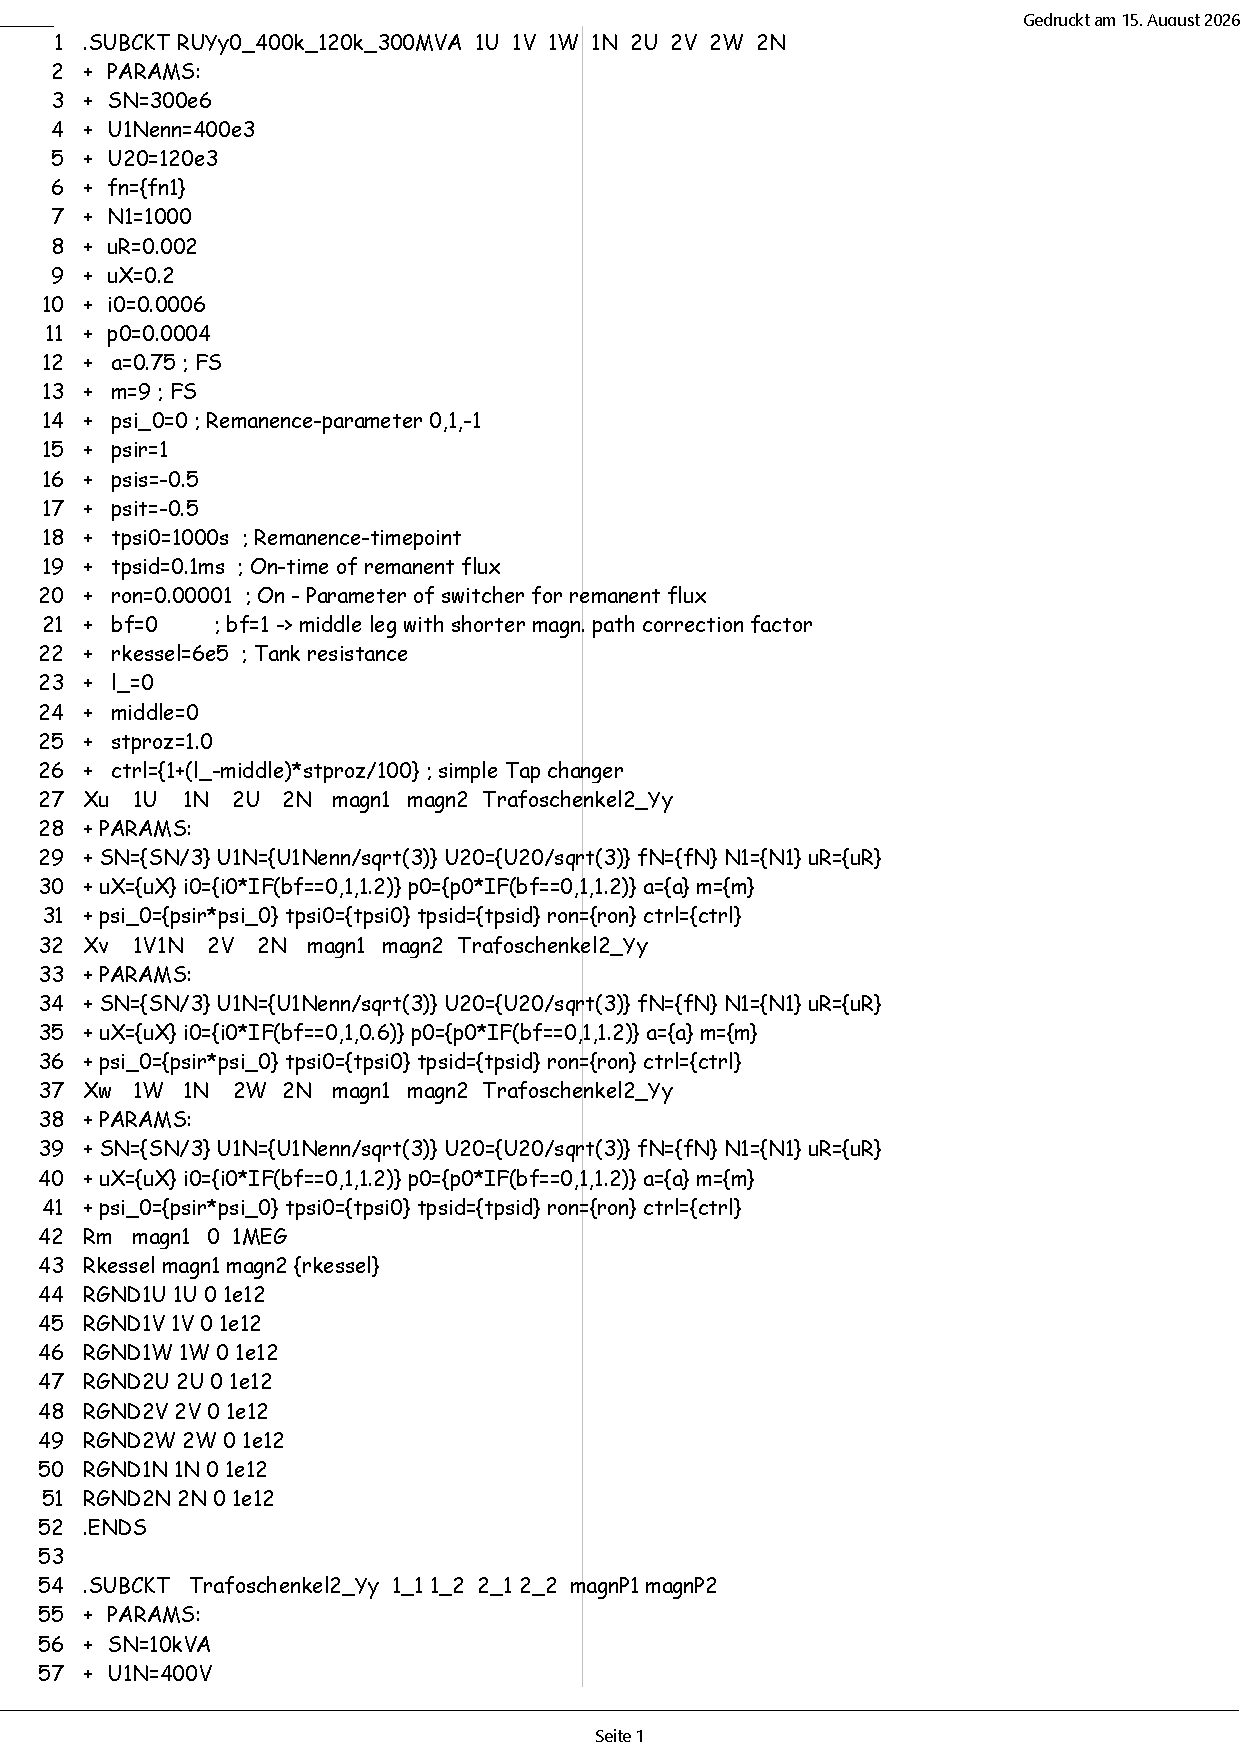
\includegraphics[width=0.90\textwidth]{figures/Transformer_SpiceCode1 1.pdf}
%	\caption{Spice code for transformer model Page1 of 3}
%	\label{fig:Transformer_and_shunt_reactor_AC_Waveform}
%\end{figure}
%
%\begin{figure}[H]
%	\centering
%	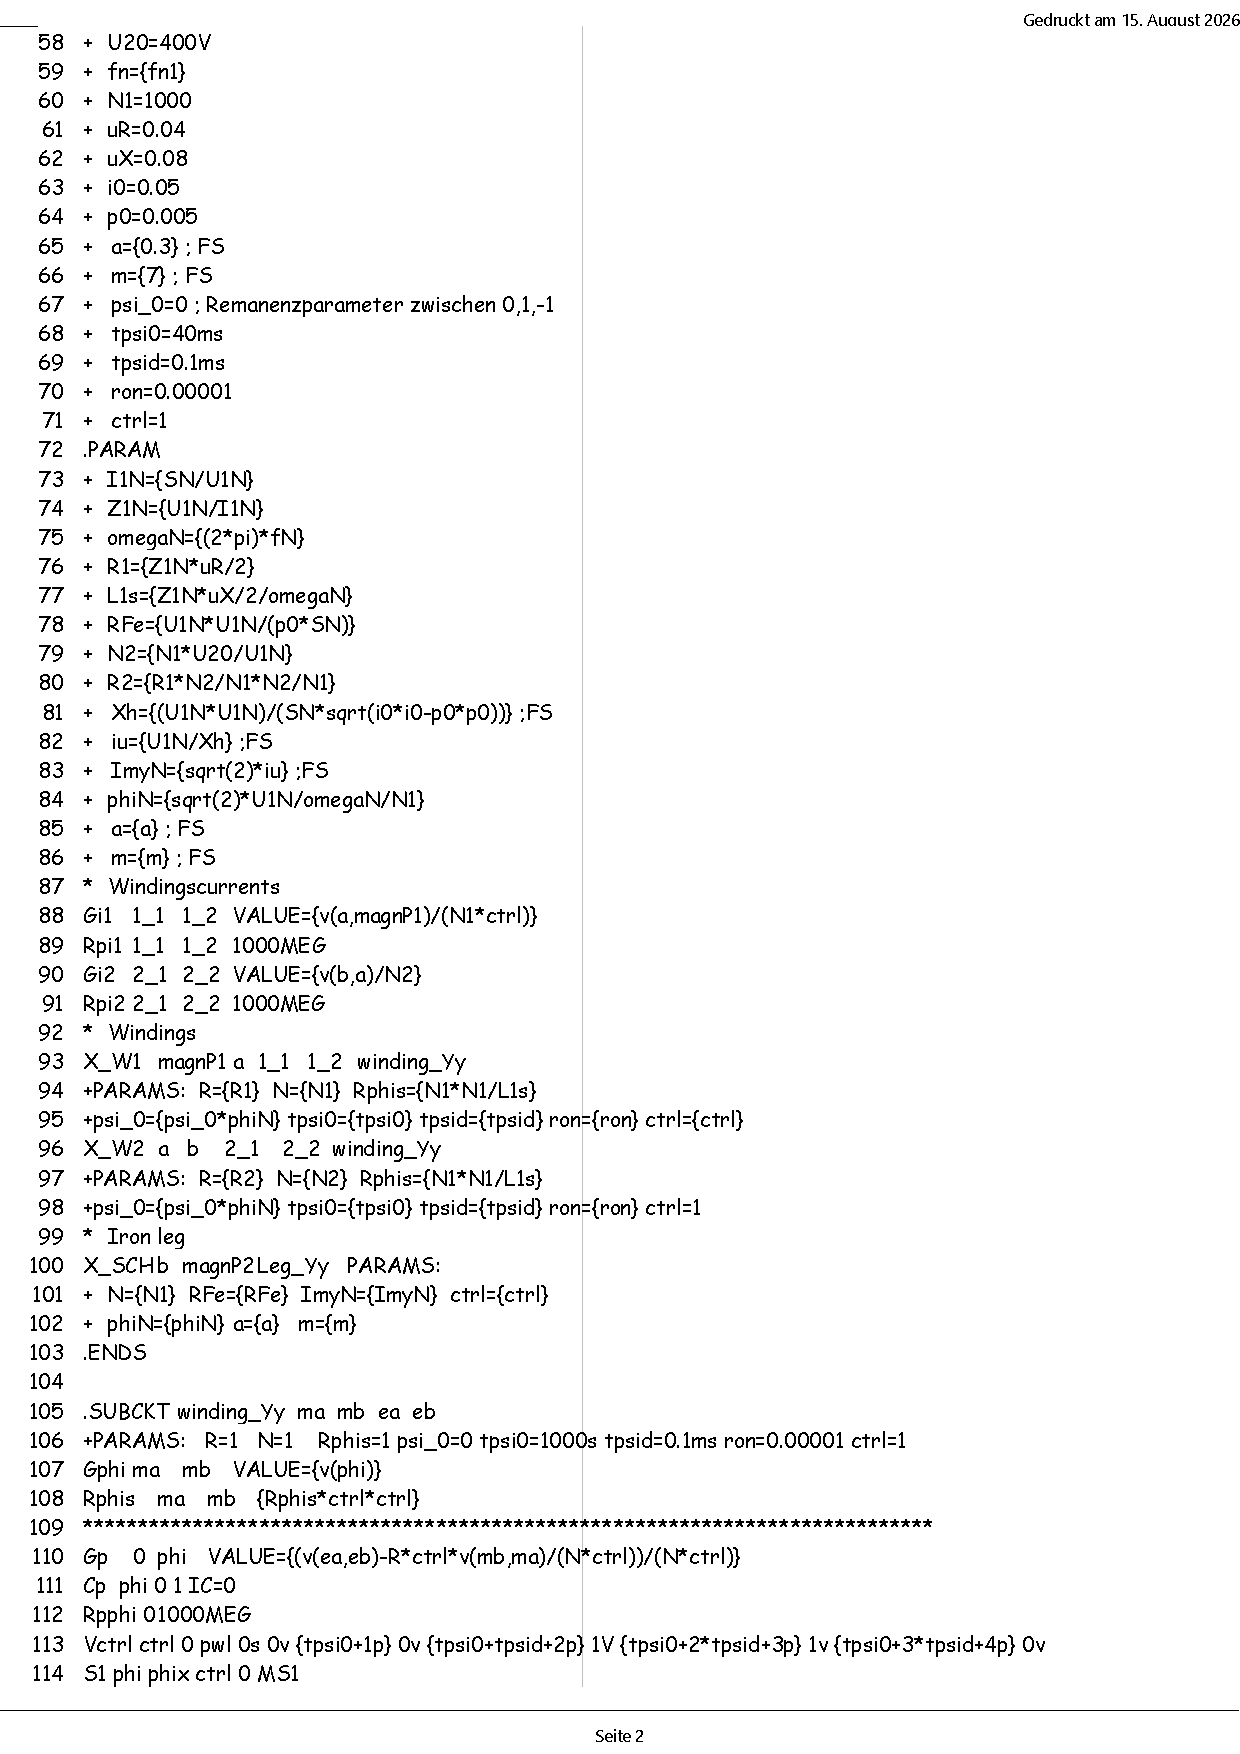
\includegraphics[width=0.90\textwidth]{figures/Transformer_SpiceCode1 2.pdf}
%	\caption{Spice code for transformer model Page2 of 3}
%	\label{fig:Transformer_and_shunt_reactor_AC_Waveform}
%\end{figure}
%
%\begin{figure}[H]
%	\centering
%	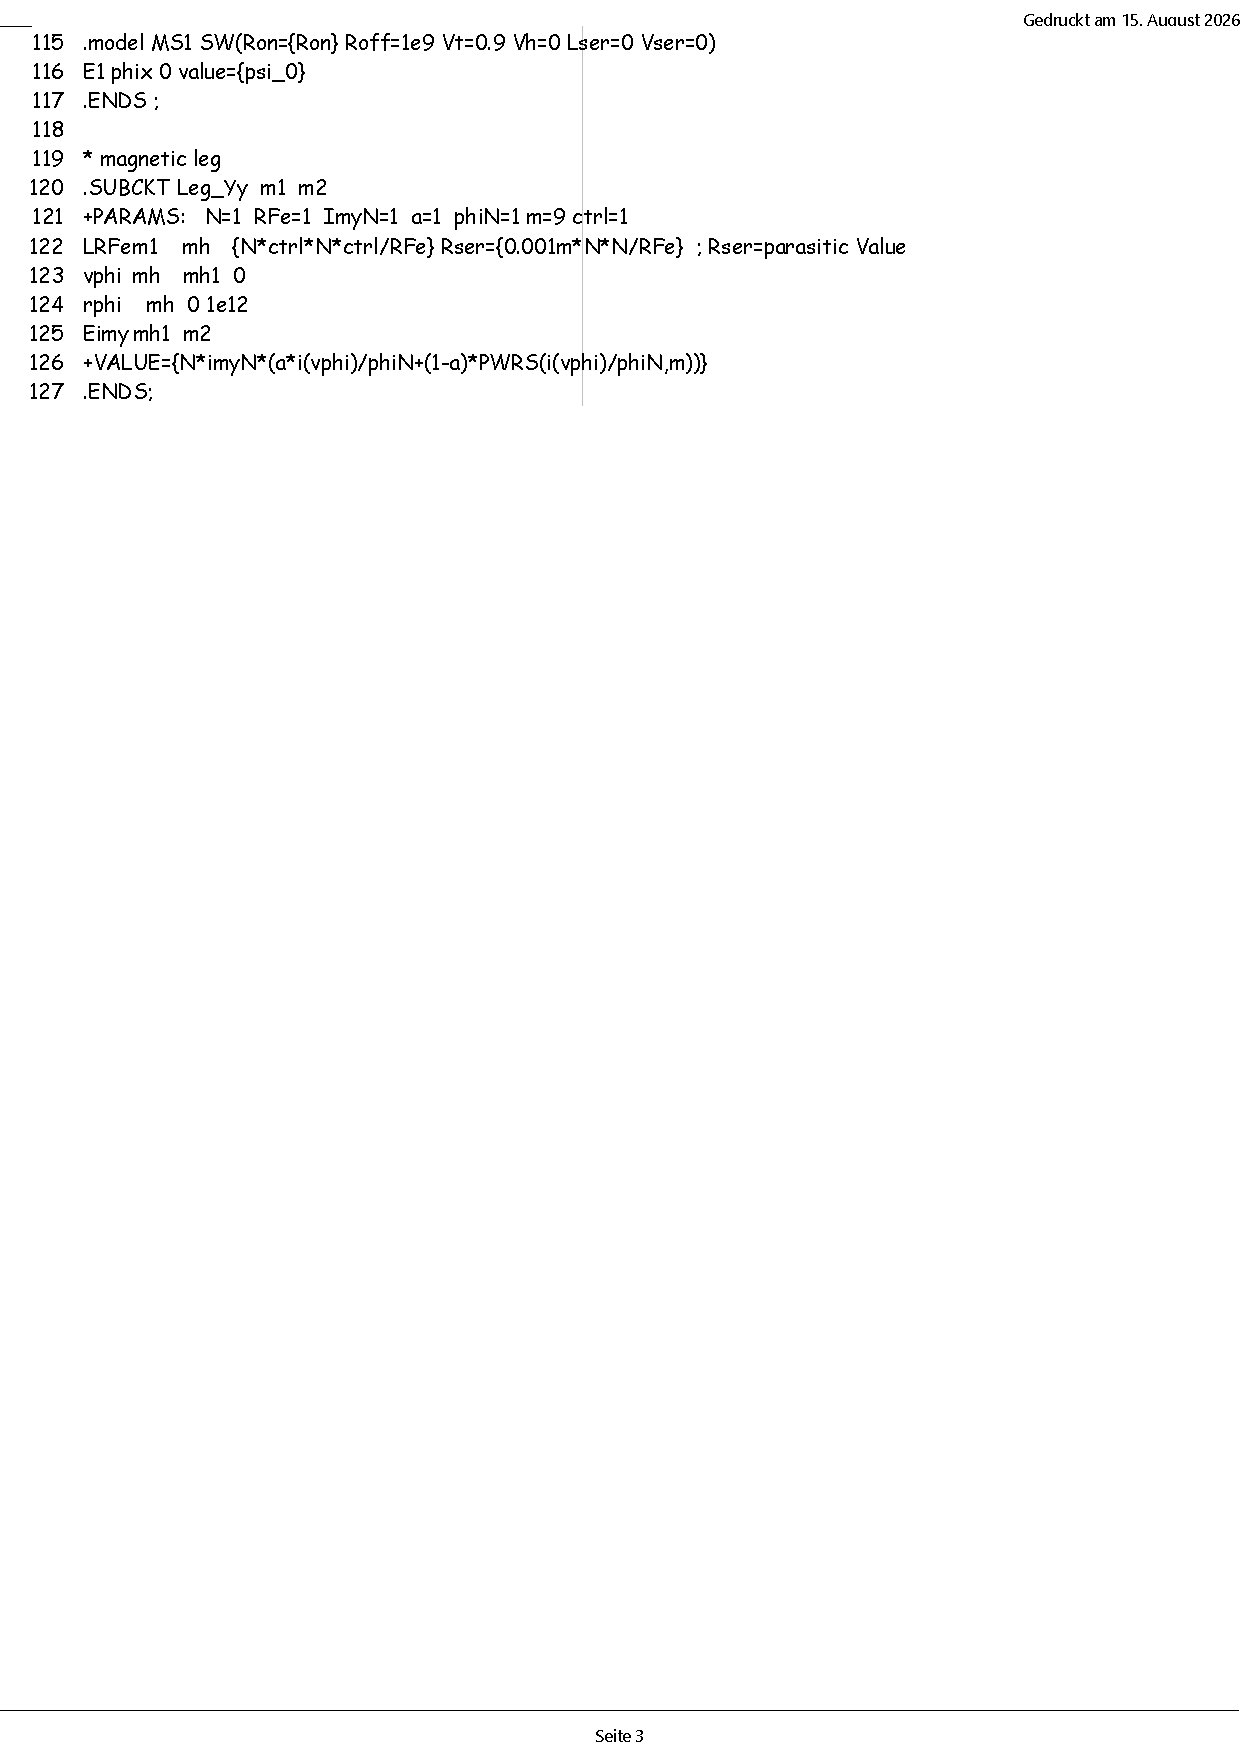
\includegraphics[width=0.90\textwidth]{figures/Transformer_SpiceCode1 3.pdf}
%	\caption{Spice code for transformer model Page3 of 3}
%	\label{fig:Transformer_and_shunt_reactor_AC_Waveform}
%\end{figure}


	

\chapter[Behavioral Sources in LTspice]
{Mathematical Modelling with Behavioral Sources in LTspice}
\label{app:behavioral-sources}
\index{LTspice!behavioral source}
\index{behavioral source}
\index{controlled source}

\section{Behavioral E and G Sources}
\label{sec:behavioral-eg-sources}

Behavioral voltage and current sources make it possible to implement
mathematical models directly in LTspice. Node voltages, branch currents,
parameters, arithmetic operations, logical operations, and built-in functions
can be combined in one expression.

\begin{formulaBox}{Basic LTspice syntax}
An E source generates a voltage between its output nodes:
\begin{lstlisting}[style=LTspice]
E1 node1 node2 VALUE={mathematical_expression}
\end{lstlisting}

A G source generates a branch current between its output nodes:
\begin{lstlisting}[style=LTspice]
G1 node1 node2 VALUE={mathematical_expression}
\end{lstlisting}

Typical expression operands are
\begin{lstlisting}[style=LTspice]
V(node)              ; node voltage relative to ground
V(node_plus,node_minus) ; differential node voltage
I(Vsense)             ; current through a voltage source
Ix(U1:pin)            ; current into a subcircuit pin
\end{lstlisting}
\end{formulaBox}

\begin{noteBox}
\textbf{Elements used in the toolboxes.}
The principal element designators are
\texttt{V}, \texttt{I}, \texttt{L}, \texttt{C}, \texttt{R}, \texttt{K},
\texttt{E}, \texttt{G}, \texttt{S}, \texttt{T}, and \texttt{O}.
Consult the LTspice help for the precise syntax, sign convention, and analysis
restrictions of each element.
\end{noteBox}

\begin{important}{Dimensional consistency}{imp:behavioral-source-units}
The value returned by an E-source expression is interpreted as volts; the
value returned by a G-source expression is interpreted as amperes. LTspice
does not enforce physical dimensional consistency inside a behavioral
expression. The model author must therefore verify all scaling factors and
units.
\end{important}

\section{Functions in Behavioral Expressions}
\label{sec:behavioral-functions}

The following functions can be used in behavioral E and G sources. Optional
arguments are shown in square brackets. Function availability can depend on the
installed LTspice version.

\begingroup
\small
\setlength{\LTpre}{0pt}
\setlength{\LTpost}{6pt}
\renewcommand{\arraystretch}{1.12}
\begin{longtable}{>{\ttfamily\raggedright\arraybackslash}p{0.31\textwidth}
                  >{\raggedright\arraybackslash}p{0.61\textwidth}}
\caption{Functions available in LTspice behavioral expressions.}
\label{tab:ltspice-behavioral-functions}\\
\toprule
\normalfont\bfseries Function & \bfseries Description \\
\midrule
\endfirsthead
\caption[]{Functions available in LTspice behavioral expressions (continued).}\\
\toprule
\normalfont\bfseries Function & \bfseries Description \\
\midrule
\endhead
\midrule
\multicolumn{2}{r}{\small Continued on next page}\\
\endfoot
\bottomrule
\endlastfoot
abs(x) & Absolute value of $x$. \\
absdelay(x,t[,tmax]) & Delays $x$ by $t$; the optional maximum delay is \texttt{tmax}. \\
acos(x) & Real part of the arc cosine. For example, \texttt{acos(-5)} returns \texttt{3.14159}, not a complex result. \\
arccos(x) & Synonym for \texttt{acos(x)}. \\
acosh(x) & Real part of the inverse hyperbolic cosine. \\
asin(x) & Real part of the arc sine. Out-of-domain arguments are limited to the real result. \\
arcsin(x) & Synonym for \texttt{asin(x)}. \\
asinh(x) & Inverse hyperbolic sine. \\
atan(x) & Arc tangent of $x$. \\
arctan(x) & Synonym for \texttt{atan(x)}. \\
atan2(y,x) & Four-quadrant arc tangent of $y/x$. \\
atanh(x) & Inverse hyperbolic tangent. \\
buf(x) & Returns 1 if $x>0.5$; otherwise returns 0. \\
cbrt(x) & Real cube root of $x$. \\
ceil(x) & Smallest integer greater than or equal to $x$. \\
cos(x) & Cosine of $x$; the argument is in radians. \\
cosh(x) & Hyperbolic cosine of $x$. \\
ddt(x) & Time derivative $\diff x/\diff t$. \\
delay(x,t[,tmax]) & Same as \texttt{absdelay(x,t[,tmax])}. \\
dnlim(x,A,Delta) & Smooth approximation of \texttt{max(x,A)} with first-derivative transition width $\Delta$. \\
exp(x) & Exponential function $\mathrm{e}^{x}$. \\
floor(x) & Largest integer less than or equal to $x$. \\
hypot(x,y) & Returns $\sqrt{x^2+y^2}$ with suitable numerical scaling. \\
idt(x[,ic[,a]]) & Integrates $x$; \texttt{ic} is the optional initial condition and the integrator is reset when \texttt{a} is true. \\
idtmod(x[,ic[,m[,o]]]) & Integrates $x$, resets on reaching modulus \texttt{m}, and offsets the output by \texttt{o}. \\
if(x,y,z) & Returns $y$ if $x>0.5$; otherwise returns $z$. \\
int(x) & Converts $x$ to an integer. \\
inv(x) & Returns 0 if $x>0.5$; otherwise returns 1. \\
limit(x,y,z) & Returns the intermediate value of $x$, $y$, and $z$. \\
ln(x) & Natural logarithm of $x$. \\
log(x) & Alternate syntax for \texttt{ln(x)}. \\
log10(x) & Base-10 logarithm of $x$. \\
max(x,y) & Greater of $x$ and $y$. \\
min(x,y) & Smaller of $x$ and $y$. \\
mod(x,y) & Remainder of the division $x/y$. \\
noise() & Returns 1 during a \texttt{.noise} analysis; otherwise returns 0. \\
pow(x,y) & Real part of $x^y$; for example, \texttt{pow(-1,0.5)} returns 0 rather than an imaginary value. \\
pwr(x,y) & Returns $|x|^y$. \\
pwrs(x,y) & Returns $\operatorname{sgn}(x)|x|^y$. \\
rand(x) & Pseudorandom value between 0 and 1 determined by the integer value of $x$. \\
random(x) & Similar to \texttt{rand(x)}, but transitions smoothly between values. \\
round(x) & Integer nearest to $x$. \\
sdt(x[,ic[,assert]]) & Alternate syntax for \texttt{idt(x[,ic[,assert]])}. \\
sgn(x) & Sign of $x$: $-1$, 0, or 1. \\
sin(x) & Sine of $x$; the argument is in radians. \\
sinh(x) & Hyperbolic sine of $x$. \\
smallsig() & Returns 1 during a \texttt{.ac} or \texttt{.noise} analysis; otherwise returns 0. \\
square(x) & Returns $x^2$. \\
sqrt(x) & Square root of $x$. \\
table(x,a,b,c,d,...) & Linearly interpolates a value for $x$ from the point pairs $(a,b),(c,d),\ldots$. \\
table(x, .include ``filename'') & Interpolates from point pairs stored as numbers in an included file. \\
tan(x) & Tangent of $x$. \\
tanh(x) & Hyperbolic tangent of $x$. \\
u(x) & Unit step: 1 if $x>0$; otherwise 0. \\
uplim(x,A,Delta) & Smooth approximation of \texttt{min(x,A)} with first-derivative transition width $\Delta$. \\
uramp(x) & Returns $x$ if $x>0$; otherwise returns 0. \\
white(x) & Pseudorandom value between $-0.5$ and $0.5$ with smoother transitions than \texttt{random(x)}. \\
xor(x,y) & Converts $x$ and $y$ to Boolean values and returns their exclusive OR. \\
!(x) & Alternate syntax for \texttt{inv(x)}. \\
\textasciitilde(x) & Alternate syntax for \texttt{inv(x)}. \\
\end{longtable}
\endgroup

\section{Operators and Precedence}
\label{sec:behavioral-operators}

Table~\ref{tab:ltspice-operators} lists the behavioral-expression operators in
ascending order of precedence. Operators in the same group have equal
precedence; parentheses should be used whenever the intended evaluation order
could be ambiguous.

\begingroup
\small
\renewcommand{\arraystretch}{1.14}
\begin{longtable}{>{\ttfamily\raggedright\arraybackslash}p{0.19\textwidth}
                  >{\raggedright\arraybackslash}p{0.73\textwidth}}
\caption{LTspice behavioral-expression operators in ascending order of precedence.}
\label{tab:ltspice-operators}\\
\toprule
\normalfont\bfseries Operator & \bfseries Description \\
\midrule
\endfirsthead
\caption[]{LTspice behavioral-expression operators (continued).}\\
\toprule
\normalfont\bfseries Operator & \bfseries Description \\
\midrule
\endhead
\bottomrule
\endfoot
\& & Converts both operands to Boolean values and returns logical AND. \\
| & Converts both operands to Boolean values and returns logical OR. \\
\textasciicircum & Converts both operands to Boolean values and returns logical XOR. \\
>, < & Greater-than and less-than comparisons. \\
>=, <= & Greater-than-or-equal and less-than-or-equal comparisons. \\
== & Returns true if both expressions are equal. \\
!=, <> & Returns true if both expressions are unequal. \\
+, - & Floating-point addition and subtraction. \\
*, / & Floating-point multiplication and division. \\
\% & Floating-point remainder; equivalent to \texttt{mod(x,y)}. \\
** & Raises the left operand to the power of the right operand. Only the real part is returned. \\
!, \textasciitilde & Unary Boolean inversion of the following expression. \\
\end{longtable}
\endgroup

\begin{noteBox}
\textbf{Boolean conversion.}
For the behavioral functions \texttt{buf()}, \texttt{if()}, and
\texttt{inv()}, LTspice treats values greater than 0.5 as true. The exact
threshold behavior of logical operators should be checked when expressions can
take non-binary analog values.
\end{noteBox}

\section{Example: Single-Phase Transformer}
\label{sec:behavioral-transformer-example}

The example implements the voltage equations by numerical integration and
solves the flux-current relations as a simultaneous linear system.

\subsection{Differential equations}

The winding-voltage equations are
\begin{align}
u &= R_1 i_1+\frac{\diff\psi_1}{\diff t},\\
0 &= (R_2+R_{\mathrm{load}})i_2
     +\frac{\diff\psi_2}{\diff t}.
\end{align}

Consequently,
\begin{align}
\frac{\diff\psi_1}{\diff t}&=u-R_1i_1,\\
\frac{\diff\psi_2}{\diff t}&=-(R_2+R_{\mathrm{load}})i_2.
\end{align}

\subsection{Flux-current equations}

The coupled linear system is
\begin{equation}
\begin{bmatrix}\psi_1\\\psi_2\end{bmatrix}
=L_{1h}
\begin{bmatrix}
1+\sigma_1 & 1\\
1 & 1+\sigma_2
\end{bmatrix}
\begin{bmatrix}i_1\\i_2\end{bmatrix}.
\label{eq:behavioral-transformer-matrix}
\end{equation}

Equivalently, the two residual equations are
\begin{align}
0&=\psi_1-(1+\sigma_1)L_{1h}i_1-L_{1h}i_2,\\
0&=\psi_2-L_{1h}i_1-(1+\sigma_2)L_{1h}i_2.
\end{align}

\subsection{LTspice netlist}

\begin{lstlisting}[style=LTspice,caption={Behavioral implementation of a single-phase transformer.},label={lst:behavioral-transformer}]
* Single-phase transformer using behavioral sources
* Parameters
.PARAM U=20 R1=10 R2=8 R_Last=17
.PARAM L1h=0.1 sigma1=0.1 sigma2=0.15

* Integrator for flux psi1.
* G-C-R realization is used because idt() can be less robust.
Gpsi1  0 psi1 VALUE={ U - R1*V(i1) }
Cpsi1  psi1 0 1 IC=0
Rpsi1  psi1 0 1E6

* Integrator for flux psi2
Gpsi2  0 psi2 VALUE={ -(R2+R_Last)*V(i2) }
Cpsi2  psi2 0 1 IC=0
Rpsi2  psi2 0 1E6

* Simultaneous linear system
Gi1  0 i1 VALUE={ V(psi1)
+ (-(1+sigma1)*L1h*V(i1)-L1h*V(i2)) }
Ri1  i1 0 1E12

Gi2  0 i2 VALUE={ V(psi2)
+ (-L1h*V(i1)-(1+sigma2)*L1h*V(i2)) }
Ri2  i2 0 1E12

.TRAN 0.001 0.04 0 0.001 UIC
\end{lstlisting}

\begin{remark}{Solution of the algebraic system}{rem:behavioral-linear-system}
The resistances \texttt{Ri1} and \texttt{Ri2} are set to
\SI{1e12}{\ohm}. The G-source currents can therefore produce only negligible
node voltages unless their behavioral expressions are nearly zero. During each
Newton iteration, LTspice consequently adjusts \texttt{V(i1)} and
\texttt{V(i2)} until both residual equations are satisfied simultaneously.
The node voltages thus represent the calculated currents $i_1$ and $i_2$.
\end{remark}

\begin{important}{Numerical interpretation of the G-C-R integrator}{imp:gcr-integrator}
With \texttt{Cpsi1=1 F}, the capacitor relation gives
$\diff V(\texttt{psi1})/\diff t=I(\texttt{Gpsi1})$, so the node voltage
directly represents flux linkage. The parallel \SI{1}{\mega\ohm} resistor
provides a DC path but also introduces a small leakage term. Increase its value
if this artificial decay is significant, while retaining a sufficiently robust
DC operating point.
\end{important}

\begin{chaptersummary}[Appendix Summary]
Behavioral E and G sources allow differential equations, algebraic equations,
logical functions, and lookup tables to be implemented directly in LTspice.
E sources return voltages, whereas G sources return currents. Integrators may
be formed either with \texttt{idt()} or explicitly with a G-C-R network. A
simultaneous algebraic system can be solved by expressing each residual with a
behavioral G source and forcing it toward zero through a very large shunt
resistance. Careful attention to sign conventions, units, damping, and
operator precedence is essential for numerically robust models.
\end{chaptersummary}

\chapter[Installing LTspice and the Toolboxes]
{Download and Installation of LTspice and the Power-System Toolboxes}
\label{app:LTspice-installation}
\index{LTspice!installation}
\index{toolbox!transient simulation}
\index{toolbox!load-flow simulation}

\section{Purpose and Required Downloads}
\label{sec:LTspice-downloads}

The examples in this book use LTspice Version 24.0.12 together with two
power-system toolboxes:

\begin{itemize}
\item \textbf{Transient toolbox:}
      models and examples for electromagnetic transient simulations of
      high-energy power networks;
\item \textbf{Steady-state toolbox:}
      models and examples for load-flow and steady-state simulations.
\end{itemize}

This book concentrates on transient simulations. The steady-state toolbox is
optional and is required only when the corresponding load-flow models are to
be used.

\begin{formulaBox}{Files to download}
Download the following archive from the project homepage:
The transient and loadflow Toolboxes and the LTspice 24.0.12 simulator installation file in one archive \texttt{LTspice.zip};
The archive is large because it also contains the now free MicroCap12 simulator with Library file for loadflow and transient simulation and with some examples! This file seems a little messy because it's the development version.\\ 
 
If you only need the LTspice toolbox files preferably option is to download the archive from the LTspice usergroup in the files-z\_yahoo
section \texttt{adventures with loadflow}. NOTE: The LTspice simulator 24.0.12 must be downloading separately 

Project homepage:
\begin{lstlisting}[style=PlainText]
my homepage: <www.friedrichschmidt.at>  or 
LTspice usergroup files at: <https://groups.io/g/LTspice/files/z_yahoo/adventures%20with%20loadflow>
\end{lstlisting}
\end{formulaBox}

\begin{important}{Version used by this book}{imp:LTspice-version}
The models and screenshots described in this book were prepared for LTspice
Version 24.0.12. Newer releases may have problems displaying simulation results
in the waveform viewer. Retain the 24.0.12 installer
if exact reproducibility is required.
\end{important}

\section{Installing LTspice 24.0.12}
\label{sec:installing-LTspice}

\begin{enumerate}
\item Extract the downloaded LTspice archive to a temporary folder.
\item Right-click the installer and select \textsc{Run as administrator}.
\item Complete the installation using the default installation options.
\item Start LTspice once and close it again before copying the toolboxes. This
      confirms that the simulator has been installed correctly and allows it
      to create its normal user configuration files.
\end{enumerate}

\begin{noteBox}
\textbf{Administrator rights.}
Administrator rights are required only for the LTspice installation when the
installer writes to protected Windows folders. The toolbox files themselves
are installed in the user's Documents folder and should normally not require
administrator rights.
\end{noteBox}

\section{Installing the Toolboxes}
\label{sec:installing-power-system-toolboxes}

In the paths below, replace \texttt{<username>} with the actual Windows user
name. Extract the transient toolbox into

\begin{lstlisting}[style=PlainText]
C:\Users\<username>\Documents\LTspice
\end{lstlisting}

After extraction, the transient-toolbox folder must be

\begin{lstlisting}[style=PlainText]
C:\Users\<username>\Documents\LTspice\loadflow_transient
\end{lstlisting}

If the steady-state toolbox is also required, extract it so that the following
folder exists:

\begin{lstlisting}[style=PlainText]
C:\Users\<username>\Documents\LTspice\loadflow_steady_state
\end{lstlisting}

\begin{important}{Check the extracted folder level}{imp:toolbox-folder-level}
Avoid an additional, duplicated directory level such as
\path{LTspice\LTspice\loadflow_transient}.
The search paths configured in LTspice must point directly to the folders that
contain the toolbox symbols and library files.
\end{important}

\begin{noteBox}
\textbf{Updating an existing installation.}
If a toolbox folder already exists, make a backup before extracting a newer
archive. This preserves locally modified symbols, models, plot settings, and
example circuits.
\end{noteBox}

\section{Configuring Search Paths}
\label{sec:LTspice-search-paths}

Start LTspice and open the configuration dialog with

\begin{center}
\textsc{Tools} $\rightarrow$ \textsc{Control Panel}.
\end{center}

Open the \textsc{Sym. \& Lib. Search Paths} tab. Add the transient-toolbox path
to both the \textbf{Symbol Search Path} and the \textbf{Library Search Path}:


\begin{lstlisting}[style=PlainText]
C:\Users\<username>\Documents\LTspice\loadflow_transient
\end{lstlisting}

Thus, the same path is entered twice: once in each of the two search-path
lists.

If the steady-state toolbox is installed, also add

\begin{lstlisting}[style=PlainText]
C:\Users\<username>\Documents\LTspice\loadflow_steady_state
\end{lstlisting}

to both search-path lists.

\newpage

\begin{figure}[htbp]
	\centering
	\includegraphics[height=.3\textheight]{searchpath.jpg}
	\caption{Symbol and Library search path tab }
	\label{fig:petersen-starpoint-phasor}
\end{figure}

\begin{table}[htbp]
\centering
\caption{Required LTspice symbol and library search paths.}
\label{tab:LTspice-toolbox-search-paths}
\renewcommand{\arraystretch}{1.15}
\begin{tabularx}{\textwidth}{>{\bfseries}p{0.23\textwidth} X c}
\toprule
Toolbox & Folder & Add to both lists \\
\midrule
Transient &
\path{C:\Users\<username>\Documents\LTspice\loadflow_transient} & Yes \\
Steady state &
\path{C:\Users\<username>\Documents\LTspice\loadflow_steady_state} & Yes \\
\bottomrule
\end{tabularx}
\end{table}

\section{Configuring the Simulator}
\label{sec:LTspice-control-panel-settings}

Keep the Control Panel open and configure the following tabs.

\subsection{SPICE tab}

Set the numerical solver to

\begin{center}
\textbf{Solver: Alternate}.
\end{center}

The alternate solver is recommended for the large networks, nonlinear magnetic
models, switches, and behavioral equations used in the transient toolbox.

\begin{figure}[htbp]
	\centering
	\includegraphics[height=.3\textheight]{spice.jpg}
	\caption{Spice tab}
	\label{fig:spicetab}
\end{figure}

\newpage
\subsection{Save Defaults tab}

Enable the first three checkboxes on this tab. The exact labels can vary
slightly between LTspice builds. These options ensure that the internal data
required by many toolbox plots and hierarchical models are retained.

\begin{figure}[htbp]
	\centering
	\includegraphics[height=.3\textheight]{savedefaults.jpg}
	\caption{Save defaults tab}
	\label{fig:savedefaultstab}
\end{figure}


\begin{noteBox}
\textbf{Internal subcircuit quantities.}
Several examples inspect internal transformer fluxes, winding currents, or
hierarchical node voltages. If these traces are unavailable, return to
\textsc{Save Defaults} and verify that the relevant subcircuit node voltages
and currents are saved.
\end{noteBox}

\newpage

\subsection{Schematic tab}

\begin{figure}[htbp]
	\centering
	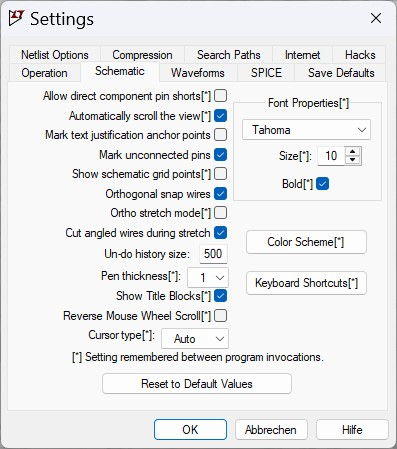
\includegraphics[height=.3\textheight]{Schematic.jpg}
	\caption{Schematic tab}
	\label{fig:Schematictab}
\end{figure}


Set the schematic-editor font to

\begin{center}
\textbf{Arial, 10 pt, Bold}.
\end{center}

\subsection{Waveforms tab}

Set the waveform-viewer font to

\begin{center}
\textbf{Arial, 12 pt,   Data trace width=2,   Cursor width=2}.
\end{center}

\begin{figure}[htbp]
	\centering
	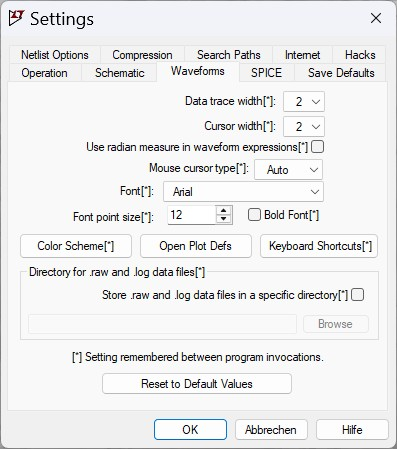
\includegraphics[height=.3\textheight]{Waveform.jpg}
	\caption{Waveforms tab}
	\label{fig:waveformtab}
\end{figure}

\subsection{Operation tab}

Enable the following options:

\begin{itemize}
\item \textbf{Marching Waveforms};
\item \textbf{Generate Expanded Listing};
\item \textbf{Save all open files on start of simulation};
\item \textbf{Automatically Delete .raw Files}.
\end{itemize}

\begin{figure}[htbp]
	\centering
	\includegraphics[height=.3\textheight]{operation.jpg}
	\caption{Operation tab}
	\label{fig:Operationtab}
\end{figure}

\begin{remark}{Automatically deleting RAW files}{rem:delete-raw-files}
RAW files from long transient simulations can become very large. Automatic
deletion saves disk space after the waveform window is closed. Disable this
option temporarily if a RAW file must be retained for later evaluation or
shared with another user.
\end{remark}

\begin{table}[htbp]
\centering
\caption{Summary of the recommended LTspice settings.}
\label{tab:recommended-LTspice-settings}
\renewcommand{\arraystretch}{1.16}
\begin{tabularx}{\textwidth}{>{\bfseries}p{0.24\textwidth} X}
\toprule
Control Panel tab & Recommended setting \\
\midrule
Sym. \& Lib. Search Paths & Add each installed toolbox folder to both the
symbol and library search-path lists. \\
SPICE & Solver: \textbf{Alternate}. \\
Save Defaults & Enable the first three checkboxes. \\
Drafting Options & Arial, 10 pt, Bold. \\
Waveforms & Arial, 10 pt, Bold. \\
Operation & Enable Marching Waveforms, Generate Expanded Listing, and
Automatically Delete .raw Files. \\
\bottomrule
\end{tabularx}
\end{table}

\section{Verifying the Installation}
\label{sec:verify-LTspice-toolboxes}

After closing the Control Panel, restart LTspice and perform the following
checks:

\begin{enumerate}
\item Open the component-selection dialog and verify that toolbox symbols can
      be selected.
\item Open one transient-toolbox example circuit.
\item Confirm that LTspice reports no missing symbol or library-file errors.
\item Run a short transient analysis.
\item Verify that the waveform viewer opens and that hierarchical quantities
      required by the example can be selected.
\item If the steady-state toolbox is installed, open and run one of its
      load-flow examples as a separate check.
\end{enumerate}

\begin{important}{If models or symbols are not found}{imp:toolbox-not-found}
Check the spelling of the Windows user name, confirm the extracted folder
level, and verify that the toolbox path was entered in both search-path lists.
After changing a search path, restart LTspice before testing the installation
again.
\end{important}

\begin{chaptersummary}[Appendix Summary]
Install LTspice 24.0.12 with its default options, extract the transient toolbox
to the user's Documents folder, and optionally install the steady-state
load-flow toolbox. Add every installed toolbox folder to both the symbol and
library search paths. Use the alternate solver, save the internal model data
required by the examples, configure consistent schematic and waveform fonts,
and enable the recommended operating options. A short example simulation
should be run after installation to verify that all symbols and library models
are available.
\end{chaptersummary}

\chapter[Q\&A: Transient Simulation]
{Questions and Answers for Transient Simulation}
\label{app:qa-transient-simulation}
\index{transient simulation!questions and answers}
\index{LTspice!troubleshooting}

This appendix collects practical questions that frequently arise when using
the transient-simulation toolbox. The answers refer to the conventions and
models used in this book.

\section{Basic Simulation Setup}

\begin{formulaBox}{Which parameters should be present on every schematic?}
The following global parameters are recommended:
\begin{lstlisting}[style=LTspice]
.param tdv=1 tdt=1
.param fn1=50 omega_n={2*pi*fn1}
.options vntol=1m abstol=1u
\end{lstlisting}

Use \texttt{fn1=60} for a \SI{60}{\hertz} system. The values
\texttt{vntol=1m} and \texttt{abstol=1u} correspond to
\SI{1}{\milli\volt} and \SI{1}{\micro\ampere}; they are included in the
toolbox template \texttt{template.asc}.

For a \SIrange{50}{60}{\hertz} system, a useful maximum transient time step is
between \SI{0.1}{\milli\second} and \SI{0.6}{\milli\second}. A smaller step
improves temporal resolution but increases simulation time. The alternate
solver is recommended under \textsc{Tools} $\rightarrow$
\textsc{Control Panel} $\rightarrow$ \textsc{SPICE}.

If a result is physically implausible, first check transformer orientation and
all engineering prefixes. In LTspice, \texttt{m} means milli; use
\texttt{Meg} for mega. A value of \texttt{400} means \SI{400}{\volt}, not
\SI{400}{\kilo\volt}.
\end{formulaBox}

\begin{formulaBox}{How can steady state be reached quickly?}
The voltage-source parameters \texttt{texp} and \texttt{tpwl} can be used to
ramp the source voltage. Values between approximately
\SI{10}{\milli\second} and \SI{100}{\milli\second} normally produce a final
voltage buildup over roughly \SIrange{50}{500}{\milli\second}.

Transformer energization can additionally be improved by coordinating the
residual-flux parameter \texttt{psi\_0} with the switching instant. For a
phase-R voltage zero crossing followed by a positive voltage half-cycle:
\begin{itemize}
\item \texttt{psi\_0=-1} can place the flux close to its steady-state path;
\item \texttt{psi\_0=0} can produce approximately twice rated peak flux;
\item \texttt{psi\_0=1} can produce approximately three times rated peak flux.
\end{itemize}
At a voltage maximum, \texttt{psi\_0=0} normally gives the smallest flux
offset. The exact polarity depends on the winding and voltage sign convention.
\end{formulaBox}

\begin{formulaBox}{What can be done if the circuit does not converge?}
Use the following sequence:
\begin{enumerate}
\item Verify units, polarities, initial conditions, floating nodes, and switch
      timing.
\item Reduce the maximum time step.
\item Use the alternate solver.
\item Provide realistic parasitic resistances and DC paths.
\item If necessary, relax \texttt{vntol}, \texttt{abstol}, or
      \texttt{reltol} moderately.
\end{enumerate}
Increasing tolerances can help convergence but reduces numerical accuracy;
repeat the final simulation with tighter tolerances as a check.
\end{formulaBox}

\begin{formulaBox}{How can subcircuit currents and voltages be accessed?}
Open
\begin{center}
\textsc{Tools} $\rightarrow$ \textsc{Control Panel} $\rightarrow$
\textsc{Save Defaults}
\end{center}
and enable \textbf{Save Subcircuit Node Voltages} and
\textbf{Save Subcircuit Device Currents}. Restart or rerun the simulation after
changing these settings.
\end{formulaBox}

\begin{formulaBox}{How are power, energy, and current direction displayed?}
Hold \textsc{Alt} and click a component to plot its instantaneous power, based
on the voltages and currents at its pins. Hold \textsc{Ctrl} and click the
power trace label to integrate the trace over the displayed interval and obtain
energy.

LTspice defines device-pin currents as positive into the pin. Resistors,
capacitors, and inductors display a current arrow. Mirroring a symbol also
mirrors this reference direction.
\end{formulaBox}

\begin{formulaBox}{What must be considered for LTspice inductors?}
LTspice inductors may contain a default series resistance of
\SI{1}{\milli\ohm}. Right-click the inductor and set \texttt{Rser=0} if an
ideal inductor is required. The global default can be changed under
\textsc{Tools} $\rightarrow$ \textsc{Control Panel} $\rightarrow$
\textsc{Hacks} by enabling the option that defaults inductors to
\texttt{Rser=0}.

Removing all loss can create an undamped resonant circuit and may worsen
convergence. Use a physically meaningful resistance whenever possible.
\end{formulaBox}

\section{Transformer Models and Magnetic Quantities}

\begin{formulaBox}{How is a nonlinear transformer changed to a linear model?}
Right-click the transformer and set
\begin{lstlisting}[style=LTspice]
m=1
\end{lstlisting}
in the value or parameter field. This removes the high-order nonlinear term in
the toolbox magnetization characteristic.
\end{formulaBox}

\begin{formulaBox}{Which parameters determine the magnetization curve?}
The characteristic is controlled primarily by \texttt{a} and \texttt{m}:
\begin{equation}
i_\mu(\Phi)=I_{\mu N}
\left[
a\frac{\Phi}{\Phi_N}
+(1-a)\left(\frac{\Phi}{\Phi_N}\right)^m
\right].
\label{eq:qa-magnetization-curve}
\end{equation}

The parameter $a$ determines the linear share and the small-signal slope,
while $m$ controls the sharpness of saturation. Typical large-transformer
examples use $m=7$ or $m=9$. 

The quantities $I_{\mu N}$ and $\Phi_N$ must use the same amplitude convention.
If peak flux is used, the rated peak values are
\begin{equation}
\Phi_N=\frac{\sqrt{2}\,U_{N,\mathrm{ph}}}{\omega N},
\qquad
I_{\mu N}=\sqrt{2}\,I_{\mu N,\mathrm{rms}}.
\end{equation}
\end{formulaBox}

\begin{formulaBox}{How is residual flux specified?}
Use the transformer parameter \texttt{psi\_0} for a predefined residual-flux
pattern. Where supported, phase-specific parameters should be used for an
arbitrary residual-flux vector. The initialization time must match the desired
switching event.
\end{formulaBox}

\begin{formulaBox}{How is residual flux applied at an arbitrary time?}
The model briefly connects an initialization voltage source to the
\SI{1}{\farad} flux-integrator capacitor. The switch on-resistance and duration
determine the charging accuracy:
\begin{equation}
\tau=R_{\mathrm{on}}C.
\end{equation}
For example,
\begin{equation}
R_{\mathrm{on}}=10^{-5}\,\Omega,\quad C=\SI{1}{\farad}
\quad\Longrightarrow\quad
\tau=\SI{0.01}{\milli\second}.
\end{equation}
A closing duration of \SI{0.1}{\milli\second} corresponds to $10\tau$ and
charges the capacitor essentially to its final value. The rapid initialization
can produce a narrow voltage or current spike at the charging instant.
\end{formulaBox}

\begin{formulaBox}{Where can introductory LTspice tutorials be found?}
An introductory tutorial collection is available at
\url{http://www.simonbramble.co.uk/lt_spice/ltspice_lt_spice.htm}.
\end{formulaBox}

\begin{formulaBox}{How is the JUSTUS transformer model composed?}
The model combines an electrical circuit with a magnetic equivalent circuit.
Iron loss, leakage, and core paths can therefore be represented with magnetic
quantities. Under the magnetic-electrical duality used in the model:
\begin{itemize}
\item electrical series connections correspond to magnetic parallel paths;
\item electrical parallel connections correspond to magnetic series paths;
\item resistance corresponds to conductance under the chosen analogy;
\item voltage-source and current-source roles are interchanged;
\item T and $\Pi$ topologies are dual representations.
\end{itemize}

E.g to convert a inductance to a reluctance or a resistance to a reluctance for a winding with $N$ turns,
\begin{align}
\Rmag_\sigma&=\frac{N^2}{L_\sigma},\\
\Rmag_{R\mathrm{Fe}}&=\frac{N^2}{R_{\mathrm{Fe}}},
\end{align}
according to the scaling convention of the toolbox model. The placement of the
corresponding branches follows the electrical-magnetic duality described above.
\end{formulaBox}

\begin{formulaBox}{How can approximate data for a \SI{300}{\mega\volt\ampere} transformer be estimated?}
Assume a \SI{400}{\kilo\volt}/\SI{120}{\kilo\volt} Yy transformer,
$N_1=1000$, magnetic path length $l_m=\SI{10}{\metre}$, rated flux density
$B_N=\SI{1.8}{\tesla}$, and RMS magnetizing current
$I_{\mu N}=\SI{0.5}{\ampere}$.

Using RMS sinusoidal quantities,
\begin{align}
\Psi_{1N,\mathrm{rms}}
 &=\frac{U_{1N,LL}}{\sqrt{3}\,\omega}
  =\SI{735.1}{\weber},\\
\Phi_{N,\mathrm{rms}}
 &=\frac{\Psi_{1N,\mathrm{rms}}}{N_1}
  =\SI{0.7351}{\weber},\\
A_{\mathrm{Fe}}
 &=\frac{\Phi_{N,\mathrm{rms}}}{B_N}
  \approx\SI{0.408}{\metre\squared},\\
\Theta_{\mu N}&=N_1I_{\mu N}=\SI{500}{\ampere},\\
H_N&=\frac{\Theta_{\mu N}}{l_m}=\SI{50}{\ampere\per\metre},\\
\mu_r&=\frac{B_N}{\mu_0H_N}\approx2.86\times10^4,\\
\Rmag_m&=\frac{\Theta_{\mu N}}{\Phi_{N,\mathrm{rms}}}
 \approx\SI{680}{\per\henry},\\
L_{1h}&=\frac{N_1^2}{\Rmag_m}\approx\SI{1470}{\henry}.
\end{align}

The equivalent peak convention gives
$\widehat\Phi_N=\sqrt{2}\Phi_{N,\mathrm{rms}}
=\SI{1.0396}{\weber}$ and
$\widehat I_{\mu N}=\sqrt{2}I_{\mu N}$, leaving reluctance and inductance
unchanged. RMS and peak quantities must not be mixed in one calculation.
\end{formulaBox}

\begin{formulaBox}{What does the nonlinear curve predict at one, two, and three times rated flux?}
For $a=0.75$, $m=9$, and a reference current of
$I_{\mu N}=\SI{0.5}{\ampere}$ in a consistent amplitude convention,
\begin{align}
i_\mu(1\Phi_N)&=\SI{0.5}{\ampere},\\
i_\mu(2\Phi_N)&=\SI{64.75}{\ampere},\\
i_\mu(3\Phi_N)&=\SI{2461.5}{\ampere}.
\end{align}

For $l_m=\SI{10}{\metre}$ and $B_N=\SI{1.8}{\tesla}$, the corresponding
approximate magnetic quantities are
\begin{table}[H]
\centering
\renewcommand{\arraystretch}{1.12}
\begin{tabular}{ccccc}
\toprule
$\Phi/\Phi_N$ & $B$ & $H$ & $\mu_r$ & $L_{1h}$ \\
\midrule
1 & \SI{1.8}{\tesla} & \SI{50}{\ampere\per\metre} & $2.86\times10^4$ & \SI{1470}{\henry} \\
2 & \SI{3.6}{\tesla} & \SI{6475}{\ampere\per\metre} & 442 & \SI{22.7}{\henry} \\
3 & \SI{5.4}{\tesla} & \SI{2.46e5}{\ampere\per\metre} & 17.5 & \SI{0.90}{\henry} \\
\bottomrule
\end{tabular}
\end{table}

These are point estimates based on the assumed algebraic curve. In a dynamic
simulation, winding voltage drop, leakage flux, and waveform distortion reduce
the effective flux and RMS current. Even at three times rated flux, the
estimated main inductance remains above the example leakage inductance
$L_\sigma\approx\SI{0.1697}{\henry}$.
\end{formulaBox}

\begin{formulaBox}{How can tank reluctance be estimated?}
The tank path is strongly geometry- and frequency-dependent. A placeholder
inductance of a few henries, or roughly 10 to 100 times the winding leakage
inductance, may be useful for sensitivity studies, but it is not a validated
transformer parameter. Measurements or field calculations are required for an
accurate value.
\end{formulaBox}

\begin{formulaBox}{How can transformer voltage and phase be regulated?}
The rudimentary tap parameter \texttt{l\_} changes the voltage in steps. For
example, \texttt{l\_=3} and \texttt{stproz=1.5} correspond to a nominal
\SI{4.5}{\percent} change, subject to the model sign convention.

The models \texttt{trafo\_tap\_l} and \texttt{trafo\_tap\_s} provide voltage
and phase-angle regulation. Versions with fixed parameters and versions with
control pins are available; the latter can be driven by a PWL source during a
transient simulation.
\end{formulaBox}

\section{Selecting and Analysing Models}

\begin{formulaBox}{How are alternative models selected?}
Right-click the element and open the \textbf{SpiceModel} drop-down list. It
contains models from the associated \texttt{.lib} file. The model
pin count and pin order must match the symbol! 
\end{formulaBox}

\begin{formulaBox}{How is a transient model converted to AC analysis?}
Replace transient sources by sources with AC magnitude and phase definitions,
and replace the \texttt{.tran} directive by an \texttt{.ac} directive. AC
analysis linearizes the circuit about its operating point; it is generally not
suitable for studying switching events or strongly nonlinear large-signal
behaviour.
\end{formulaBox}

\begin{formulaBox}{How can reactive-power transfer be recognized?}
Reactive-power transfer produces a phase displacement between the fundamental
voltage and current. For sinusoidal RMS phasors,
\begin{equation}
Q=\sqrt{3}\,U_{LL}I_L\sin\varphi.
\end{equation}
For distorted waveforms, calculate average active power from $u(t)i(t)$ and
use a harmonic-aware definition of reactive power.
\end{formulaBox}

\begin{formulaBox}{Why do many elements have control pins?}
Control pins allow parameters such as voltage level, tap position, phase shift,
switch state, or model coefficient to change during the simulation. A PWL
source is commonly used to drive a discrete or continuous control input.
\end{formulaBox}

\section{Inductive Coupling and Flux}

\begin{formulaBox}{How is leakage between two coupled inductors calculated?}
For self-inductances $L_1,L_2$ and mutual inductance $M$,
\begin{align}
k&=\frac{M}{\sqrt{L_1L_2}},\\
\sigma&=1-\frac{M^2}{L_1L_2}=1-k^2.
\end{align}
If the individual leakage factors are $\sigma_1$ and $\sigma_2$,
\begin{equation}
\sigma=\sigma_1+\sigma_2-\sigma_1\sigma_2.
\end{equation}
For a symmetric transformer, $\sigma_1=\sigma_2$, hence
\begin{equation}
\sigma=2\sigma_1-\sigma_1^2,
\qquad k=1-\sigma_1,
\qquad L_{1\sigma}=(1-k)L_1.
\end{equation}

With $L_{1\sigma}=\SI{0.1697}{\henry}$ and
$L_1=\SI{1470}{\henry}$,
\begin{align}
\sigma_1&=1.1544\times10^{-4},\\
\sigma&=2.3087\times10^{-4},\\
k&=\boxed{0.9998846}.
\end{align}
The voltage ratio and inductances satisfy
\begin{equation}
\frac{N_1}{N_2}=\sqrt{\frac{L_1}{L_2}}
\end{equation}
when both inductances use the same magnetic path and reference convention.
\end{formulaBox}

\begin{formulaBox}{What is the rated peak flux for 1000 turns?}
For sinusoidal phase voltage $U_{N,\mathrm{ph}}$,
\begin{equation}
\widehat\Psi_N=\frac{\sqrt{2}\,U_{N,\mathrm{ph}}}{\omega},
\qquad
\widehat\Phi_N=\frac{\widehat\Psi_N}{N}.
\end{equation}

At \SI{50}{\hertz} and $N=1000$:
\begin{table}[H]
\centering
\renewcommand{\arraystretch}{1.12}
\begin{tabular}{lcc}
\toprule
Voltage applied to winding & Connection interpretation & $\widehat\Phi_N$ \\
\midrule
\(\SI{10}{\kilo\volt}/\sqrt{3}\) & \SI{10}{\kilo\volt} star phase & \SI{0.0260}{\weber} \\
\SI{10}{\kilo\volt} & Winding voltage & \SI{0.0450}{\weber} \\
\(\SI{20}{\kilo\volt}/\sqrt{3}\) & \SI{20}{\kilo\volt} star phase & \SI{0.0520}{\weber} \\
\SI{20}{\kilo\volt} & Winding voltage & \SI{0.0900}{\weber} \\
\(\SI{110}{\kilo\volt}/\sqrt{3}\) & \SI{110}{\kilo\volt} star phase & \SI{0.286}{\weber} \\
\SI{110}{\kilo\volt} & Winding voltage & \SI{0.495}{\weber} \\
\(\SI{220}{\kilo\volt}/\sqrt{3}\) & \SI{220}{\kilo\volt} star phase & \SI{0.572}{\weber} \\
\SI{220}{\kilo\volt} & Winding voltage & \SI{0.990}{\weber} \\
\(\SI{400}{\kilo\volt}/\sqrt{3}\) & \SI{400}{\kilo\volt} star phase & \SI{1.0396}{\weber} \\
\bottomrule
\end{tabular}
\end{table}
\end{formulaBox}

\begin{formulaBox}{What are the time constants of RL and RC circuits?}
\begin{equation}
\tau_{RL}=\frac{L}{R},
\qquad
\tau_{RC}=RC.
\end{equation}
A first-order response reaches approximately \SI{99.3}{\percent} of its final
change after $5\tau$ and \SI{99.995}{\percent} after $10\tau$.
\end{formulaBox}

\begin{formulaBox}{What do \texttt{tpsid} and \texttt{ron} mean?}
The parameter \texttt{tpsid} specifies how long the initialization source is
connected to the \SI{1}{\farad} flux-integrator capacitor. The parameter
\texttt{ron} is the switch on-resistance. Suitable example values are
\begin{lstlisting}[style=LTspice]
tpsid=0.1m  ron=1e-5
\end{lstlisting}
giving $\tau=R_{\mathrm{on}}C=\SI{0.01}{\milli\second}$ and an initialization
interval of $10\tau$.
\end{formulaBox}

\begin{formulaBox}{How can the magnetization curve be plotted?}
Open the transformer secondary. In the waveform viewer, change the horizontal
axis from time to primary current and plot internal flux or flux linkage versus
that current. A nonzero iron-loss parameter \texttt{p0} produces a loop-like
separation because the loss current is superimposed; it should not be confused
with a fully physical hysteresis model unless the model explicitly contains
hysteresis state equations.
\end{formulaBox}

\section{Lines, Cables, and Compensation}

\begin{formulaBox}{How is cable charging power calculated?}
For line-to-line RMS voltage $U_N$, phase-to-earth capacitance $C_E$, and
phase-to-phase capacitance $C_L$ per phase set,
\begin{align}
Q_0&=Q_{CE}+Q_{CL}
   =U_N^2\omega C_E+3U_N^2\omega C_L,\\
I_0&=\frac{Q_0}{\sqrt{3}U_N}.
\end{align}
For a shielded single-core cable, $C_L$ is commonly negligible and
$Q_0\approx Q_{CE}$. The capacitive earth-fault current is then approximately
\begin{equation}
I_E=3I_0=\frac{3Q_{CE}}{\sqrt{3}U_N}.
\end{equation}
\end{formulaBox}

\begin{formulaBox}{How are Petersen coils and shunt reactors sized?}
For a Petersen coil connected from the transformer neutral to earth,
\begin{align}
X_L&=\frac{U_N/\sqrt{3}}{I_N}, &
L&=\frac{X_L}{\omega}.
\end{align}
For an example with $U_N=\SI{110}{\kilo\volt}$ and
$I_N=\SI{250}{\ampere}$, the coil loss may initially be estimated with
$R\approx X_L/100$ and later replaced by measured data.

For a three-phase reactor with total rating $Q_N$:
\begin{align}
L_\Delta&=\frac{3U_N^2}{\omega Q_N},\\
L_Y&=\frac{U_N^2}{\omega Q_N}.
\end{align}
Each delta branch sees $U_N$, whereas each star branch sees $U_N/\sqrt{3}$.

If $C_E=\SI{1000}{\nano\farad}$ at \SI{110}{\kilo\volt},
\begin{align}
Q_0&=U_N^2\omega C_E\approx\SI{3.80}{\mega\varunit},\\
I_0&=\frac{Q_0}{\sqrt{3}U_N}\approx\SI{19.95}{\ampere},\\
I_E&=3I_0\approx\SI{59.85}{\ampere}.
\end{align}
A Petersen coil rated approximately \SI{110}{\kilo\volt} and
\SI{60}{\ampere} therefore provides the required compensation.
\end{formulaBox}

\begin{formulaBox}{How does coupling influence parallel lines?}
Lines on the same route have mutual inductive and capacitive coupling. Depending
on current direction and phase arrangement, mutual induction can reduce or
increase the effective series inductance. In the idealized same-direction case,
$k\rightarrow1$ makes the differential leakage inductance approach zero.

The toolbox contains coupled-line models for one, two, and four circuits. Their
coupling matrices were calculated with ATP/ATPDraw and converted to LTspice
format with the supplied Excel conversion file.
\end{formulaBox}

\begin{formulaBox}{How is source impedance obtained from short-circuit power?}
For a balanced three-phase network,
\begin{equation}
Z_N=\frac{U_N^2}{S_k}.
\end{equation}
Examples are
\begin{align}
U_N=\SI{400}{\kilo\volt},\quad S_k=\SI{40}{\giga\volt\ampere}
&\Rightarrow Z_N=\SI{4.0}{\ohm},\\
U_N=\SI{110}{\kilo\volt},\quad S_k=\SI{7.5}{\giga\volt\ampere}
&\Rightarrow Z_N=\SI{1.613}{\ohm}.
\end{align}
If no resistance information is available, the first approximation is an
inductive source impedance $jX_N$ with $X_N\approx Z_N$.
\end{formulaBox}

\begin{formulaBox}{How is the total capacitance of an overhead line calculated?}
With phase-to-earth capacitance $C_E$ and phase-to-phase capacitance $C_L$, the
effective positive-sequence charging capacitance is
\begin{equation}
C_{\mathrm{sum}}=C_E+3C_L.
\end{equation}
The capacitive reactive power is
\begin{equation}
Q_C=U_N^2\omega C_{\mathrm{sum}}
   =\frac{U_N^2}{X_C}.
\end{equation}
\end{formulaBox}

\begin{formulaBox}{How is the reactive power of a shunt reactor calculated?}
For a balanced three-phase reactor connected in star,
\begin{equation}
Q_L=\frac{U_N^2}{X_L}
   =\frac{U_N^2}{\omega L},
\end{equation}
where $L$ is the inductance of each phase branch.
\end{formulaBox}

\begin{formulaBox}{What is the difference between star and delta loads with identical branch impedances?}
If the same branch resistance or impedance is used in both connections at the
same line-to-line voltage, each delta branch receives $\sqrt{3}$ times the star
branch voltage. Therefore,
\begin{equation}
P_\Delta=3P_Y,
\qquad Q_\Delta=3Q_Y.
\end{equation}
\end{formulaBox}

\section{Plot Files and Verification}

\begin{formulaBox}{How is a saved plot configuration displayed?}
Many examples include saved plot-setting files. In the waveform viewer, use
\textsc{Plot Settings} $\rightarrow$ \textsc{Open Plot Settings} and select
the required file. If several configurations are supplied, open them one at a
time to reproduce the intended trace groups.
\end{formulaBox}

\begin{formulaBox}{How should a transient simulation be verified?}
Always repeat the simulation with a smaller maximum time step. A credible
result should change only slightly as the time step is reduced. Also check:
\begin{itemize}
\item energy and power balance;
\item expected steady-state RMS values and phase sequence;
\item sensitivity to tolerances and parasitic resistances;
\item agreement between transient, AC, and hand calculations where applicable;
\item correct current reference directions and voltage bases;
\item plausibility of resonant frequencies and decay time constants.
\end{itemize}
\end{formulaBox}

\begin{chaptersummary}[Appendix Summary]
Reliable transient simulation begins with consistent global parameters,
correct units, suitable time steps, and physically meaningful damping. Source
ramps and coordinated residual flux reduce initialization transients, while
the alternate solver and carefully selected tolerances improve numerical
robustness. Every important result should be repeated with a
smaller time step and compared with analytical estimates.
\end{chaptersummary}

\chapter[LTspice Schematic Editor]
{LTspice Schematic Editor: Menu Bar, Toolbar, and Basic Operation}
\label{app:LTspice-schematic-editor}
\index{LTspice!schematic editor}
\index{LTspice!toolbar}

\begin{figure}[htbp]
  \centering
  \IfFileExists{LTspice_editor_annotated.pdf}{%
    \includegraphics[width=\textwidth]{LTspice_editor_annotated.pdf}%
  }{%
    \IfFileExists{figures/LTspice_editor_annotated.pdf}{%
      \includegraphics[width=\textwidth]{figures/LTspice_editor_annotated.pdf}%
    }{%
      \fbox{\parbox[c][55mm][c]{0.92\textwidth}{\centering
      Copy \texttt{LTspice\_editor\_annotated.pdf} into the same directory as
      this \LaTeX{} file or into the book's \texttt{figures} directory.}}
    }%
  }
  \caption{Annotated LTspice 24 schematic-editor window showing the title and
  menu bars, functional toolbar groups, schematic drawing area, grid, and
  status bar. The appearance of individual icons depends on the selected
  toolbar style and LTspice version.}
  \label{fig:LTspice-editor}
\end{figure}

\begin{noteBox}{Version note:}
This overview refers to the Windows schematic editor used in LTspice 24.0.12.
The illustration shows the default LTspice 24 toolbar. Users who prefer the
older, smaller icon set can select the legacy toolbar with
\textsc{Tools} $\rightarrow$ \textsc{Settings} $\rightarrow$
\textsc{Operation} $\rightarrow$ \textsc{Toolbar Style} $\rightarrow$
\textsc{Legacy}.
\end{noteBox}


\section{Main Areas of the Schematic Editor}

\begin{formulaBox}{1. Menu bar}
The menu bar provides access to all drawing, simulation, display, and program
configuration commands. Toolbar icons are available for the most commonly used commands.
\end{formulaBox}

\begin{formulaBox}{2. Toolbar}
The toolbar gives direct access to frequently used commands such as opening a
schematic, starting a simulation, inserting components, drawing wires, and
editing circuit elements. Moving the mouse pointer over an icon displays its
function as a tooltip.
\end{formulaBox}

\begin{formulaBox}{3. Drawing area}
Components, wires, node labels, comments, and SPICE directives are placed in
the drawing area. The electrical reference node must be the ground node named
\texttt{0}. A schematic without node \texttt{0} normally cannot be simulated.
\end{formulaBox}

\section{Menu Bar}

\small
\begin{tabularx}{\textwidth}{>{\bfseries}p{24mm} X}
\toprule
Menu & Purpose \\
\midrule
File & Creates, opens, closes, saves, and prints schematic files. It also
       provides access to recently used files and program exit. \\
Edit & Contains undo and editing operations such as delete, duplicate, move,
       stretch, rotate, mirror, search, and selection commands. \\
Hierarchy & Creates and manages hierarchical blocks, symbols, ports, and
       multi-level schematics. \\
View & Controls zoom, grid, anchors, unconnected-pin markers, netlist display,
       SPICE error log, and other schematic or waveform views. \\
Simulate & Starts, pauses, or stops a simulation and opens the dialog for
       defining transient, AC, DC, noise, and operating-point analyses. \\
Tools & Opens program settings and provides component, symbol, and library
       management functions. \\
Window & Selects and arranges open schematic, waveform, and text windows. \\
Help & Opens the LTspice documentation, keyboard-shortcut information, and
       version information. \\
\bottomrule
\end{tabularx}
\normalsize

\section{Toolbar Symbols}

\small
\begin{tabularx}{\textwidth}{>{\bfseries}p{34mm} >{\ttfamily}p{17mm} X}
\toprule
Command & Shortcut & Function \\
\midrule
New Schematic & Ctrl+N & Creates a new empty schematic. \\
Open & Ctrl+O & Opens an existing schematic or supported LTspice file. \\
Save & Ctrl+S & Saves the active schematic. \\
Control Panel / Settings & --- & Opens the general LTspice configuration. \\
Run & --- & Starts the selected simulation. \\
Stop / Halt & --- & Stops the active simulation. \\
Zoom Area & Ctrl+Z & Enlarges a rectangular part of the schematic. \\
Zoom Back & Ctrl+B & Returns to the preceding zoom level. \\
Zoom to Fit & Space & Fits the complete schematic into the window. \\
Wire & F3 & Draws an electrical connection between nodes. \\
Ground & G & Places the mandatory reference node \texttt{0}. \\
Label Net & F4 & Assigns a name to a node or electrical network. \\
Component & F2 & Opens the component and symbol selection dialog. \\
Resistor & R & Places a resistor. \\
Capacitor & C & Places a capacitor. \\
Inductor & L & Places an inductor. \\
Diode & D & Places a diode. \\
SPICE Directive & S & Places commands such as \texttt{.tran}, \texttt{.param},
  \texttt{.options}, or \texttt{.measure}. \\
Text Comment & T & Places explanatory text without electrical effect. \\
Delete & F5 & Deletes selected components, wires, labels, or text. \\
Duplicate / Copy & F6 & Creates a copy of the selected object. \\
Move & F7 & Moves an object; connected wires are not stretched with it. \\
Stretch / Drag & F8 & Moves an object while retaining and adapting its wires. \\
Rotate & Ctrl+R & Rotates the selected component by 90 degrees. \\
Mirror & Ctrl+E & Mirrors the selected component. \\
Undo & F9$^{*}$ & Reverses the last editing action. \\
\bottomrule
\end{tabularx}

\normalsize
\medskip
\noindent\footnotesize
$^{*}$ The effective shortcut can depend on the active window and the configured
hotkeys. LTspice displays the currently assigned keys in its menus and tooltips.
\normalsize

\section{Basic Workflow}

\begin{formulaBox}{Creating and simulating a circuit}
\begin{enumerate}
  \item Create or open a schematic.
  \item Insert the required components and assign their parameters.
  \item Connect the circuit with the \textsc{Wire} tool.
  \item Insert ground node \texttt{0} and assign useful net labels.
  \item Define the simulation with
        \textsc{Simulate} $\rightarrow$ \textsc{Configure Analysis} or place the
        corresponding SPICE directive directly on the schematic.
  \item Press \textsc{Run} and select node voltages or branch currents in the
        waveform viewer.
\end{enumerate}
\end{formulaBox}

\begin{noteBox}{Move and Stretch:}
\textsc{Move} changes the position of a component without preserving the exact
wire geometry. \textsc{Stretch} moves the component together with its connected
wires. Press \texttt{Esc} or the right mouse button to leave an active
editing mode.
\end{noteBox}

\section{References}

\begin{itemize}
  \item Analog Devices,
  \href{https://www.analog.com/en/resources/media-center/videos/6368296317112.html}%
  {``LTspice Basics: Schematic Capture.''}
  \item Analog Devices EngineerZone, information about the LTspice 24 toolbar
  and the legacy toolbar style,
  \href{https://ez.analog.com/design-tools-and-calculators/LTspice/f/q-a/581713/tool-bar-is-incomplete}%
  {``Toolbar is Incomplete.''}
  \item Interface illustration adapted from the LTspice schematic-entry
  tutorial by LEnsE, Institut d'Optique Graduate School,
  \href{https://lense.institutoptique.fr/mine/LTspice-saisir-un-schema/}%
  {``LTspice: Schematic Entry.''}
\end{itemize}



\begin{figure}[htbp]
	\centering
	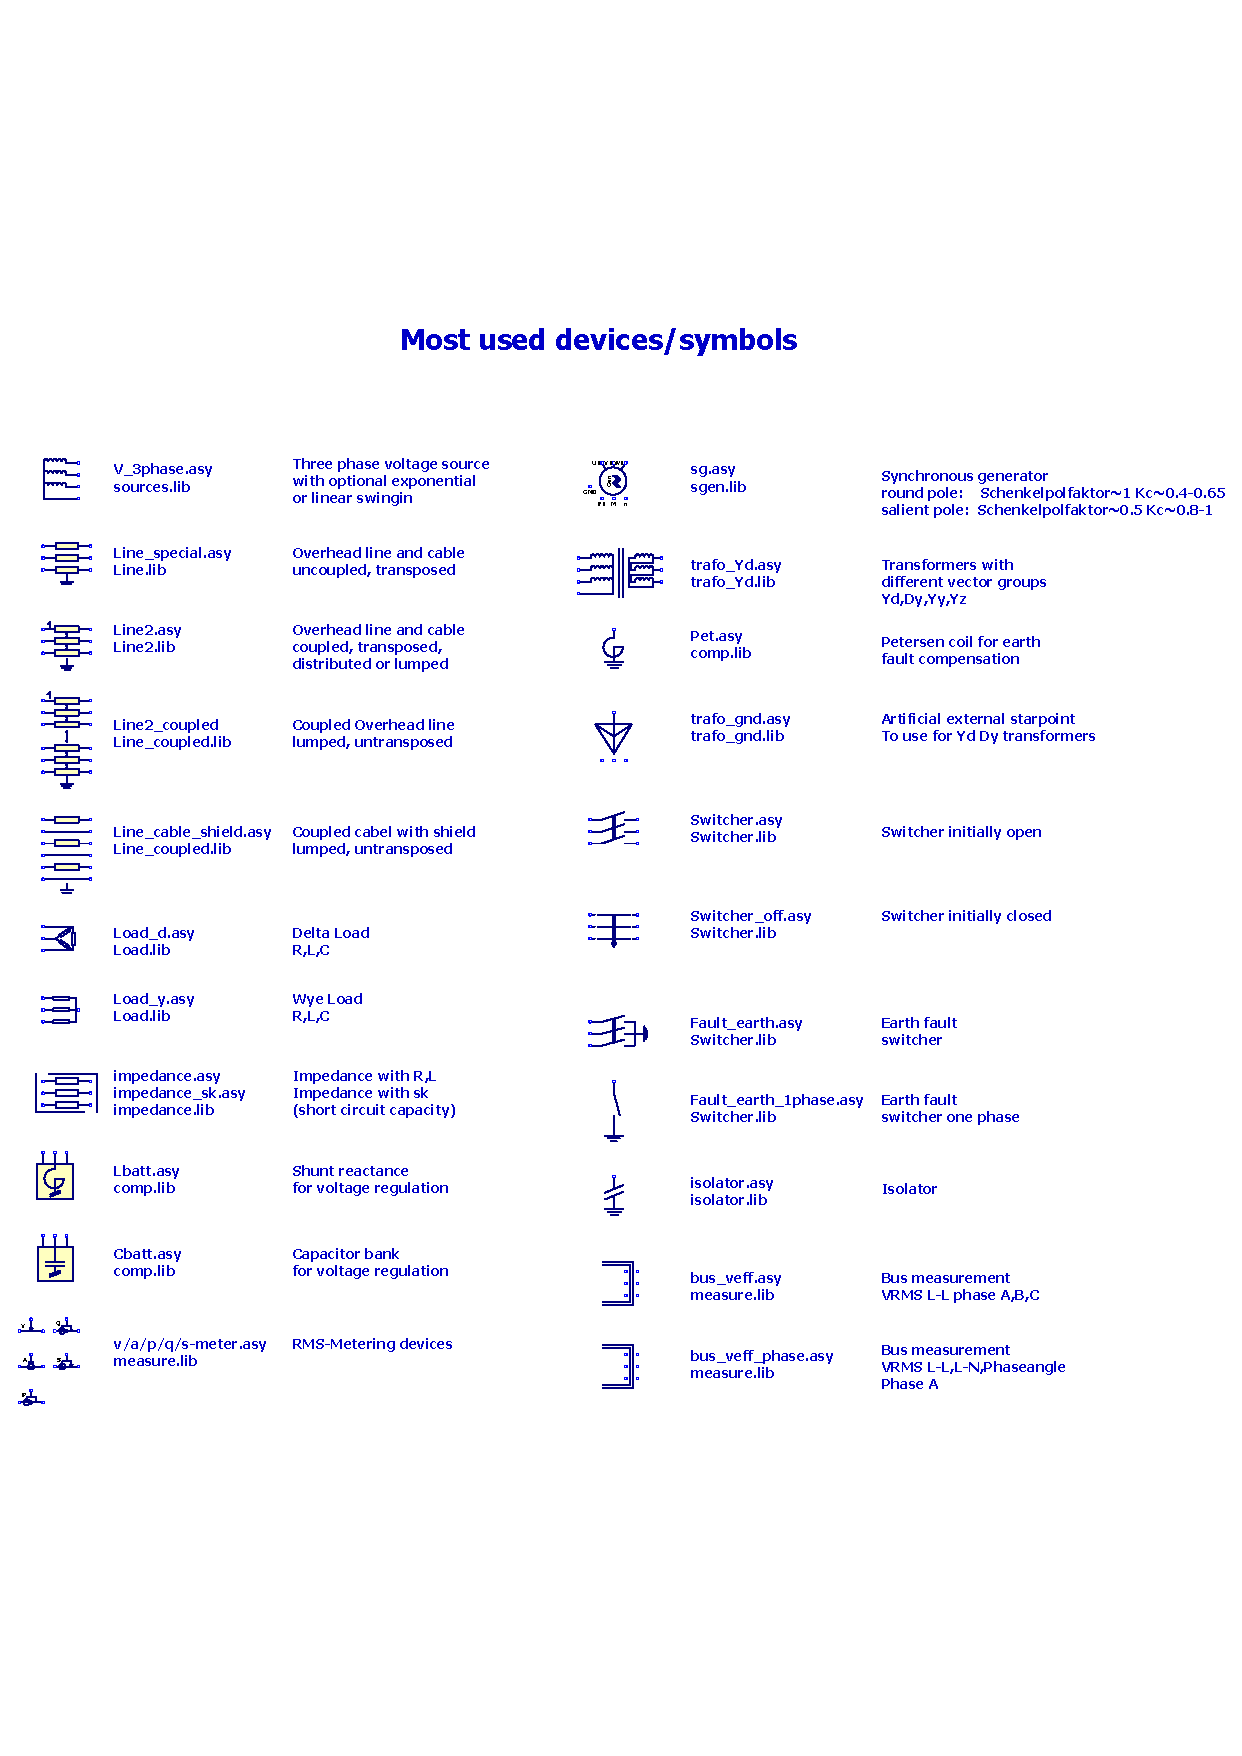
\includegraphics[height=1\textheight]{figures/Symbols_most_used.pdf}
	\caption{Most used symbols for transient toolbox}
	\label{fig:petersen-starpoint-phasor}
\end{figure}
% ============================================================
% Back matter
% ============================================================
\backmatter
\printbibliography[heading=bibintoc,title={References}]
Over the past 25 years, I have developed many macromodels for LTspice. This work resulted in two toolboxes: one for nonlinear load-flow calculations and one for transient simulations of electrical power networks. Adapting a SPICE simulator for nonlinear load-flow calculations  (with a mathematical trick) was an important part of this development.
Both toolboxes are intended for educational use, especially by students of electrical engineering. Their source files are freely available, together with hundreds of examples. This book focuses on transient simulations of electrical power networks with a detailed description and simulation of 9 handpicked examples.
The transient toolbox includes the essential components needed to model power systems: voltage sources, synchronous generators with saturation, nonlinear transformers with residual-flux initialisation and phase-angle regulation, Petersen coils for earth-fault compensation, shunt reactors, loads, overhead lines and cables, coupled lines, grounding transformers and many other components.
LTspice is a simulator developed by Analog Devices and is available free of charge. Having worked for more than 35 years as a load dispatcher in Vienna’s electricity distribution system, I have drawn on my practical experience in developing these toolboxes.
I hope that you enjoy exploring electrical power systems through simulation as much as I do. Some simulations can be challenging, but the results offer valuable insights. Good luck with your simulations!

%@manual{ltspice,
	%  title        = {LTspice Documentation},
	%  organization = {Analog Devices},
	%  note         = {Software documentation}
	%}


@book{kundur1994,
	author    = {Prabha Kundur},
	title     = {Power System Stability and Control},
	publisher = {McGraw-Hill},
	year      = {1994}
}

@book{Otto Justus,
	author    = {Otto Justus},
	title     = {Dynamisches Verhalten elektrischer Maschinen},
	publisher = {Vieweg},
	year      = {1993}
}


@book{Bödefeld; Sequenz,
	author    = {Bödefeld, Sequenz},
	title     = {Elektrische Maschinen},
	publisher = {Springer},
	year      = {1971}
}

@book{Richter,
	author    = {Richter},
	title     = {Elektrische Maschinen1},
	publisher = {Birkhäuser},
	year      = {1967}
}

@book{Fischer,
	author    = {Fischer},
	title     = {Elektrische Maschinen},
	publisher = {Carl Hanser},
	year      = {1986}	
}

@book{Hoefer; Nielinger
	author    = {Hoefer, Nielinger},
	title     = {SPICE, Analyseprogramm für elektronische Schaltungen},
	publisher = {Springer},
	year      = {1985}		
}

@book{Hosemann; Boeck,
	author    = {Hosemann, Boeck},
	title     = {Grundlagen der elektrischen Energietechnik},
	publisher = {Springer},
	year      = {1983}		
}

@book{Oeding; Oswald,
	author    = {Oeding, Oswald},
	title     = {Elektrische Kraftwerke und Netze},
	publisher = {Springer},
	year      = {2016}		
}



\cleardoublepage

\printindex
% ------------------------------------------------------------
% About the Author / Contact and Downloads
% ------------------------------------------------------------
\newpage
\section*{About the Author}

\textbf{Friedrich Schmidt} has been working for more than 25 years on the
practical modelling and simulation of electrical power systems, with a
particular focus on load-flow calculations and transient simulations.

\vspace{0.5em}

\noindent
For questions, comments, or suggestions concerning this book and the
LTspice toolboxes, he can be contacted by e-mail:

\begin{center}
	\texttt{friedrich-schmidt@gmx.at}
\end{center}

\subsection*{LTspice Toolboxes}

The LTspice toolboxes described and used throughout this book can be
downloaded free of charge from the following sources:

\begin{itemize}
	
	\item \textbf{Author's website:} to download the simulator, the toolboxes and hundreds of examples\\[2mm]
	\url{https://www.friedrichschmidt.at}
	
	\item \textbf{LTspice User Group:}\\[2mm]
	After signing in, the toolboxes with hundreds of examples can be
	downloaded from:\\
	\url{https://groups.io/g/LTspice/files/z_yahoo/adventures_with_loadflow}
	
	\item \textbf{GitHub:}\\[2mm]
	After signing in the toolboxes with the nine examples and the ltspice simulator can also be found on GitHub by searching for \texttt{LTspice loadflow}.
	
\end{itemize}

\vspace{0.5em}

\noindent
The toolboxes contain models, libraries, and numerous simulation examples
for the analysis of electrical power systems with LTspice.

 


%\clearpage
\thispagestyle{empty}

\begingroup
\setlength{\parindent}{0pt}
\sffamily

\begin{tikzpicture}[remember picture,overlay]

% Dunkelblauer Kopfbereich
\fill[BookBlueDark]
  (current page.north west)
  rectangle
  ([yshift=-108mm]current page.north east);

% Blauer Trennstreifen
\fill[BookBlue]
  ([yshift=-108mm]current page.north west)
  rectangle
  ([yshift=-112mm]current page.north east);

% Überschrift
\node[
  anchor=north west,
  text=white,
  text width=150mm,
  align=left,
  inner sep=0pt
] at ([xshift=30mm,yshift=-34mm]current page.north west) {%
  {\fontsize{28}{34}\selectfont\bfseries
   About this book\par}

  \vspace{11mm}

  {\fontsize{13.5}{19}\selectfont
   A practical introduction for everyone interested in the
   simulation of high-voltage electrical power networks.\par}
};

% Haupttext
\node[
  anchor=north west,
  text=BookGray,
  text width=150mm,
  align=left,
  inner sep=0pt
] at ([xshift=30mm,yshift=-129mm]current page.north west) {%
  \begin{minipage}{150mm}
  \fontsize{9.5}{13.2}\selectfont

  {\color{BookBlueDark}
   \fontsize{10.4}{14.4}\selectfont
   Over the past 25 years, I have developed two educational
   toolboxes for LTspice. The first supports nonlinear load-flow
   calculations; the second is designed for the transient
   simulation of electrical power networks.\par}

  \vspace{2.5mm}

  The toolboxes contain the essential components required to build
  realistic power-system models:

  \begin{itemize}
    \setlength{\itemsep}{0pt}
    \setlength{\parsep}{0pt}
    \setlength{\topsep}{1mm}
    \setlength{\partopsep}{0pt}

    \item buses and sources;
    \item synchronous machines and transformers;
    \item overhead lines and power cables;
    \item loads and shunt reactors; and
    \item surge-protection devices, Petersen coils, and many
          other elements.
  \end{itemize}

  Some elements provide parameters that can be changed directly by
  the user. Others are supplied with carefully selected presets,
  which can also be overwridden whenever a study requires different
  values.

  \vspace{1.5mm}

  The transformer library ranges from simple models to sophisticated
  representations with a nonlinear iron core, hysteresis, and
  remanent flux. Eight vector groups and voltage levels from
  \SI{400}{\kilo\volt} down to \SI{400}{\volt} are included.
  Additional vector groups can be created by editing the
  macro-models, because all \texttt{.lib} files are freely accessible
  and editable.

  \vspace{1.5mm}

  Hundreds of examples for both toolboxes are available on my
  website, ranging from simple introductory circuits to complex
  networks. Many schematic files contain their own documentation,
  and the first nine examples are explained in detail in this book.

  \vspace{1.5mm}

  These toolboxes are intended especially for students of electrical
  engineering, but they are equally useful to teachers, engineers,
  and anyone who wants to explore power-system behaviour through
  simulation.

  \vspace{2.5mm}

  {\color{BookBlueDark}
   \fontsize{10.4}{14.4}\selectfont
   I hope you enjoy experimenting with these simulations as much as
   I do. Your feedback is always welcome.\par}
  \end{minipage}
};

% Trennlinie im Fußbereich
\draw[LightBlue,line width=0.8pt]
  ([xshift=30mm,yshift=34mm]current page.south west) --
  ([xshift=-30mm,yshift=34mm]current page.south east);

% Autor
\node[
  anchor=south west,
  text=BookBlueDark,
  inner sep=0pt,
  font=\fontsize{10.5}{15}\selectfont
] at ([xshift=30mm,yshift=23mm]current page.south west)
  {Friedrich Schmidt};

% Website
\node[
  anchor=south east,
  text=BookBlue,
  inner sep=0pt,
  font=\fontsize{10.5}{15}\selectfont\bfseries
] at ([xshift=-30mm,yshift=23mm]current page.south east)
  {www.friedrichschmidt.at};

\end{tikzpicture}

\null
\clearpage
\endgroup
\end{document}
